\documentclass[twoside,phd]{iitkgp}

\usepackage{textcomp}
\usepackage{amsfonts}
\usepackage{amssymb}
\usepackage[centertags]{amsmath}
\usepackage{enumerate}
\usepackage{graphicx}
\usepackage{adjustbox}
\usepackage{graphics}
\usepackage{multirow}
\usepackage{rotating}
\usepackage{footnote}
\usepackage{times}
\usepackage{tikz}
\usetikzlibrary{shapes,shadows,arrows}
\usepackage{lscape}
\usepackage[bottom]{footmisc}
\usepackage{enumerate}
%\usepackage{algorithm}
\usepackage{amsthm}
%\usepackage{algorithm2e}
%\usepackage[numbered]{algo}
\usepackage[T1]{fontenc}
\usepackage{color}
\usepackage{multirow}
%\usepackage{subfigure}
\usepackage{epigraph}
%\usepackage{caption}
%\usepackage{subcaption}
%\usepackage{subcaption}
%\captionsetup{compatibility=false}
\usepackage{subfigure}
%\usepackage{slashbox}
\usepackage{balance}
% \usepackage[noend]{algpseudocode}
 \usepackage{epstopdf}
 \usepackage{multirow}
\usepackage{rotating}
\usepackage{fontenc}
%\usepackage[demo]{graphicx}
%\usepackage{amsmath}
\usepackage{psfrag}
\usepackage{tipa}
\usepackage{amsfonts}
\usepackage{url}
\usepackage{float}
\usepackage{latexsym}
\usepackage{amsmath,amssymb}
\usepackage{dcolumn}
\usepackage{epsfig}
\usepackage{textcomp}
\usepackage{mathtools}
\usepackage{multirow}
%\usepackage{algorithm}
\usepackage{algorithmic}
\usepackage{soul}
\usepackage{color}
\usepackage{amsmath}
\usepackage{adjustbox}
%\usepackage{setspace}
%\newtheorem{theorem}{Theorem}[section]
%\newtheorem{lemma}[theorem]{Lemma}
%\newtheorem{proposition}[theorem]{Proposition}
%\newtheorem{corollary}[theorem]{Corollary}
% \usepackage{booktabs}
% \usepackage[linesnumbered,ruled,vlined]{algorithm2e}
% \usepackage{color}
% \usepackage[table,xcdraw]{xcolor}
% \usepackage{colortbl}
% \newtheorem{prop}{Proposition}
% \newtheorem{mydef}{Definition}
% \usepackage{adjustbox}
% \newcommand{\compas}{{\tt ComPAS}}
% \newcommand\TODO[1]{\textcolor{red}{#1}}
% \usepackage{multirow}
% \usepackage{hyperref}
% \usepackage[table,xcdraw]{xcolor}
\usepackage[linesnumbered,ruled,vlined]{algorithm2e}
\usepackage{color}
%\usepackage[table,xcdraw]{xcolor}
%\usepackage{colortbl}

\usepackage{adjustbox}
\newcommand{\compas}{{\tt ComPAS}}
%\newcommand\TODO[1]{\textcolor{red}{#1}}
\usepackage{multirow}
\usepackage{hyperref}
%\usepackage[table,xcdraw]{xcolor}
\usepackage{colortbl}
% \usepackage{subfig}
%\usepackage[hyphens]{url}
%\usepackage{hyperref}
%\usepackage{amsmath,amssymb}
%\usepackage{url}
\setlength{\parindent}{0in}
\usepackage{soul}
\usepackage{xcolor}


%\usepackage[backend=biber]{biblatex}
%\setcounter{biburllcpenalty}{7000}

%\usepackage[lined,algonl,algochapter,algoruled]{algorithm2e}
% these are for the algorithms style file, for writing algorithms
%\renewcommand{\algorithmicrequire}{\textbf{Input:}}
%\renewcommand{\algorithmicensure}{\textbf{Output:}}
%\renewcommand{\algorithmiccomment}[1]{\begin{small}/* #1 */\end{small}}
%\renewcommand{\algorithmiccomment}[1]{/* #1 */}
%\newcommand{\markup}[1]{{\color{blue}{#1}}}
%\graphicspath{{fig/}}


% The fancyhdr package allows you to easily customize the page header.
% The settings below produce a nice, well separated header.
\usepackage{fancyhdr}
  \fancyhead{}
  \fancyhead[LO]{\slshape \rightmark}
  \fancyhead[RO,LE]{\textbf{\thepage}}
  \fancyhead[RE]{\slshape \leftmark}
  \fancyfoot{}
  \pagestyle{fancy}
  \renewcommand{\chaptermark}[1]{\markboth{\chaptername \ \thechapter \ \ #1}{}}
  \renewcommand{\sectionmark}[1]{\markright{\thesection \ \ #1}}

% The caption package allows us to change the formatting of figure captions.
% The commands here change to the suggested caption format: single spaced and a bold tag
% Change the \DeclareCaptionFormat line below to make the captions fully bold
\usepackage{caption}
%\DeclareCaptionFormat{suggested}{\singlespace#1#2 #3\par\doublespace}
\DeclareCaptionFormat{suggested}{\singlespace \textbf{#1}\textbf{#2}#3 \doublespace}
\captionsetup{format=suggested}

%To instruct Latex to try to fit each paragraph into 1 less line
\let\markeverypar\everypar
\newtoks\everypar
\everypar\markeverypar
\markeverypar{\the\everypar\looseness=-1\relax}


%\newcommand{\captionfonts}{\small}

% The cite package cleans up the way citations are handled.  For example, it
% changes the citation [1,2,3,6,7,8,9,10,11] into [1-3,6-11].  If your advisor
% wants superscript citations, use the overcite package instead of the cite package.
\usepackage{cite}
%\usepackage[tone]{tipa}



% The makeidx package makes your index for you.  To make an index entry,
% go to the place in the book that should be referenced and type
%  \index{key}
% An index entry labeled "key" (or whatever you type) will then
% be included and point to the correct page.
\usepackage{makeidx}
\makeindex


%\usepackage[hyphens]{url}
%\urlstyle{rm}

% If you have a lot of equations, you might be interested in the amstex package.
% It defines a number of environments and macros that are helpful for mathematics.
% We don't do much math in this example, so we haven't used amstex here.
%
% To include a link in your pdf use \href{URL}{Text to be displayed}.  If your
% display text is the URL, you probably should use the \url{} command discussed
% above.
%
% To add a bookmark in the pdf you can use \pdfbookmark.  You can look up its usage
% in the hyperref package documentation
%\usepackage[bookmarksnumbered,pdfpagelabels=true,plainpages=false,colorlinks=true,
%            linkcolor=black,citecolor=black,urlcolor=blue]{hyperref}
%\usepackage[hyphenbreaks]{breakurl}

% ---------------- Fill in these fields for the preliminary pages -------------------
%
% For Senior and honors this is the year and month that you submit the thesis
% For Masters and PhD, this is your graduation date

\newcommand{\bigsize}{\fontsize{14pt}{20pt}\selectfont}

\Year{2017}
\Month{July}
\Author{Sandipan Sikdar}
\degree{Doctor of Philosophy}
% If you have a long title, split it between two lines. The \TitleBottom field defines the second line
% A two line title should be an "inverted pyramid" with the top line longer than the bottom.
\TitleTop{{\bigsize \bf Temporal Networks: }}
\TitleBottom{{\bigsize \bf Structure, Function and Applications}}

% Your research advisor
\AdvisorA{Dr. Animesh Mukherjee\\and\\Prof. Niloy Ganguly}



%%%%%%%%%%%%%%%%%%%%%%%%%%%%%%%%%%%%%%%%%%%%%%%%%%%%%%%%%%%%%%%%%%%%%%%%%%%
%%%%%%%%%%%%%%%%%%% APPROVAL BY DSC COMMITTEE %%%%%%%%%%%%%%%%%%%%%%%%%%%%%
%%%%%%%%%%%%%%%%%%%%%%%%%%%%%%%%%%%%%%%%%%%%%%%%%%%%%%%%%%%%%%%%%%%%%%%%%%%

\Approval{
\singlespace
\hspace{9cm}
%Date:\hspace{.8cm}$\backslash \ \ \ \ \  \ \backslash$ 20  \\  \\
Date:\hspace{.8cm}$/ \ \ \ \ \  \ /$ 20  \\  \\
Certified that the thesis entitled {\bf ``Temporal networks: Structure, function and applications''} 
submitted by Sandipan Sikdar to the Indian Institute
of Technology, Kharagpur, for the award of the degree of Doctor of Philosophy
has been accepted by the external examiners and that the student has successfully
defended the thesis in the viva-voce examination held today.

\vspace{0.5in}

%\noindent
%Signature:~~~~~~~~~~\hfill Signature:~~~~~\hfill Signature:\hfill~

%\noindent
%Name:~~~~~~~~~~~~~~~\hfill Name:~~~~~~~~~~\hfill Name:~~~~~\hfill~

\vspace{1in}
\noindent
(Member of DSC)~~~~~\hfill(Member of DSC)~~~~~\hfill(Member of DSC)

\vspace{0.3in}
%\hspace{2cm}
%Signature:
\vspace{0.5in}
%\hspace{2cm}
%Name:
\noindent
%\hspace{2cm}
(Member of DSC)~~~~~\hfill(Supervisor)\hfill ~~~~~~~ %(Co-Supervisor)\hfill ~~~~~~~

\vspace{0.3in}
%\hspace{2cm}
%Signature:~~~~~~~~~~~~~~~~~~\hfill Signature:\hfill ~~~

%\hspace{2cm}
%Name:~~~~~~~~~~~~~~~~~~~~~~~\hfill Name:~~~~~\hfill ~~~~

\vspace{0.5in}
%\hspace{2cm}
\noindent
(External Examiner)~~~~~~~~~\hfill(Chairman)\hfill ~~~~~~~
}



%%%%%%%%%%%%%%%%%%%%%%%%%%%%%%%%%%%%%%%%%%%%%%%%%%%%%%%%%%%%%%%%%%%%%%%%%%%
%%%%%%%%%%%%%%%%%%% CERTIFICATE BY SUPERVISOR %%%%%%%%%%%%%%%%%%%%%%%%%%%%%
%%%%%%%%%%%%%%%%%%%%%%%%%%%%%%%%%%%%%%%%%%%%%%%%%%%%%%%%%%%%%%%%%%%%%%%%%%%

\Certificate{
\noindent%
{\em This is to certify that the thesis entitled {\bf ``Temporal networks: Structure, function and applications''}, submitted by {\bf
Sandipan Sikdar} to the Indian Institute of Technology, %%@
Kharagpur, for the award of the degree of Doctor of Philosophy, is a record of bona fide %%@
research work carried out by him under my supervision and guidance.
The thesis, in my opinion, is worthy of consideration for the award of the degree of Doctor of Philosophy 
%in accordance with the regulations 
of the Institute. To the best of my knowledge, the results embodied in this thesis %%@
have not been submitted to any other University or Institute for the award of any other Degree or Diploma.} %%@

\vspace{-5mm}

\noindent \signaturebox{Animesh Mukherjee \\Assistant Professor\\CSE, IIT Kharagpur}


\noindent \signaturebox{Niloy Ganguly\\Professor\\CSE, IIT Kharagpur}\\
\hfill\hspace*{20pt}
\hfill \datebox
   %\vskip 0pt plus 2fill
    %\noindent Accepted for the Department\hfill%
    %\signaturebox{\@DepRep, \@DepRepTitle\\Department of Physics and
    %Astronomy }{} \vfill \noindent Accepted for the College\hfill
    %\signaturebox{\@Dean, \@DeanTitle \\
    %College of Mathematics and Physical Sciences}

}




%%%%%%%%%%%%%%%%%%%%%%%%%%%%%%%%%%%%%%%%%%%%%%%%%%%%%%%%%%%%%%%%%%%%%%%%%%%
%%%%%%%%%%%%%%%%%%% DECLARATION BY STUDENT %%%%%%%%%%%%%%%%%%%%%%%%%%%%%%%%
%%%%%%%%%%%%%%%%%%%%%%%%%%%%%%%%%%%%%%%%%%%%%%%%%%%%%%%%%%%%%%%%%%%%%%%%%%%

\Declaration{
\noindent
I certify that
\begin{enumerate}
\item[a.]   The work contained in this thesis is original and has been done by myself under 
the general supervision of my supervisors.
\item[b.]   The work has not been submitted to any other Institute for any degree or diploma.
\item[c.]   I have followed the guidelines provided by the Institute in writing the thesis.
\item[d.]   I have conformed to the norms and guidelines given in the Ethical Code of Conduct of the Institute.
\item[e.]   Whenever I have used materials (data, theoretical analysis, figures, and text) from other sources, I have given due credit to them by citing them in the text of the thesis and giving their details in the references.  %Further, I have taken permission from the copyright owners of the sources, whenever necessary.
\item[f.]   Whenever I have quoted written materials from other sources, I have put them under quotation marks and given due credit to the sources by citing them and giving required details in the references.
\end{enumerate}

\vspace{0.6in}

\hfill Sandipan Sikdar ~ ~ ~
}



%%%%%%%%%%%%%%%%%%%%%%%%%%%%%%%%%%%%%%%%%%%%%%%%%%%%%%%%%%%%%%%%%%%%%%%%%%%
%%%%%%%%%%%%%%%%%%% ACKNOWLEDGEMENT %%%%%%%%%%%%%%%%%%%%%%%%%%%%%%%%%%%%%%%
%%%%%%%%%%%%%%%%%%%%%%%%%%%%%%%%%%%%%%%%%%%%%%%%%%%%%%%%%%%%%%%%%%%%%%%%%%%

\Acknowledgments{

\noindent
I would like to take this opportunity express my gratitude to everybody who have inspired me and contributed directly or indirectly in realizing this
thesis. My parents have been the greatest source of inspiration and strength throughout my life and without their support and sacrifice, this thesis would never have taken shape. I would also like to thank my elder brother who has been my mentor throughout my life.     

It is impossible to express my gratitude to my supervisors, Prof.
Animesh Mukherjee and Prof. Niloy Ganguly in a few words. The long discussions with them not only helped me in formulating the problems of this thesis, but
also helped me to understand the nuances of doing research. This thesis would never have been possible without their constant support and encouragement. 
I would like to thank Dr. Matteo Marsili (ICTP, Italy) and Dr. Tyll Krueger (Wroclaw University of Science and Technology) for their guidance and support. 
I would also like to thank the members of my DSC Prof. J. Mukhopadhyay, Prof. A. Basu, Prof. D. Mukhopadhyay and Prof. A. Mukherjee  who have enriched this thesis with their insights and suggestions. 

I consider myself very fortunate to have been part of Complex Network Research Group (CNeRG). At CNeRG I have had the pleasure of knowing Parantapa Bhattacharya, Abir Dey, Surjya Ghosh, Tanmoy Chakraborty, Suman Kalyan Maity, Soumajit Pramanik, Abhik Jana, Sankarshan Mridha, Abhijnan Chakraborty, Ankan Mullick, Satadal Sengupta, Rohit Verma, Madhumita Mallick, Rijula Kar, Amrit Krishna, Mayank Singh, Subhendu Khatuya, Soumya Sarkar and Kaustav Rudra. Life would not have been same without them. I should also thank Debojyoti Kundu who has been a great roommate and a close friend.     

Lastly, this long journey has not always been smooth but has revealed to me the joy of learning and my only desire is to pursue it for the rest of my life. 

%realize that it is not success or fame but the sheer joy of learning that drives me to work every morning and my only desire is to continue it for the rest of my life.  








\medskip
\bigskip\medskip
\noindent
Sandipan Sikdar\\
Kharagpur, India\\
}

%%%%%%%%%%%%%%%%%%%%%%%%%%%%%%%%%%%%%%%%%%%%%%%%%%%%%%%%%%%%%%%%%%%%%%%%%%%
%%%%%%%%%%%%%%%%%%% Curriculam %%%%%%%%%%%%%%%%%%%%%%%%%%%%%%%%%%%%%%%
%%%%%%%%%%%%%%%%%%%%%%%%%%%%%%%%%%%%%%%%%%%%%%%%%%%%%%%%%%%%%%%%%%%%%%%%%%%

\Curriculams{

\noindent Sandipan Sikdar has received his B-Tech. degree in 2012 from Computer Science and Engineering department of Institute of Engineering and Management, Kolkata. He has been pursuing Ph.D. at the Department of Computer Science and Engineering, IIT Kharagpur, since
December 2012. 
  


\singlespace
\begin{center}
\vspace{0.3cm}
{\bfseries {\large Publications from the Thesis
}}
\vspace{0.3cm}
\end{center}

\begin{enumerate}
\item  {\bf Sandipan Sikdar}, Matteo Marsili, Niloy Ganguly and Animesh Mukherjee. `` On predicting long-term impact of papers: A Case Study of the Scientific Peer-Review System of the Journal of High Energy Physics''. (communicated)
\item  {\bf Sandipan Sikdar}, Tanmoy Chakraborty, Soumya Sarkar, Niloy Ganguly and Animesh Mukherjee. ``ComPAS: Community Preserving Sampling for Streaming Graphs''. 17th Conference on Autonomous Agents and MultiAgent Systems (AAMAS), Stockholm, Sweden, 2018 (accepted).
%\item  Sandipan Sikdar, Matteo Marsili and Animesh Mukherjee. ``Unsupervised Ranking of Clustering Algorithms by INFOMAX''. (communicated)
\item  {\bf Sandipan Sikdar}, Nitesh Sekhar, Matteo Marsili, Niloy Ganguly and Animesh Mukherjee. `` On the effectiveness of multiple reviewers in a peer-review system: A case study of two high impact Physics journals''. (communicated)
 \item  {\bf Sandipan Sikdar}, Matteo Marsili, Niloy Ganguly and Animesh Mukherjee. `` Influence of Reviewer Interaction Network on Long-term Citations: A Case Study of the Scientific Peer-Review System of the Journal of High Energy Physics'', 17th ACM/IEEE Joint Conference on Digital Libraries (JCDL), Toronto, Canada, 2017. 
   \item  Marcin Bodych, Niloy Ganguly, Tyll Kruger, Animesh Mukherjee, Rainer Seigmund-Schultze and {\bf Sandipan Sikdar}. `` Threshold based epidemic dynamics in systems with memory'', Europhysics Letters, 116.4(2017):48004. 
   \item  {\bf Sandipan Sikdar}, Matteo Marsili, Niloy Ganguly and Animesh Mukherjee. `` Anomalies in the peer-review system: A case study of the journal of High Energy Physics'', 25th ACM International Conference on Information and Knowledge Management (CIKM), Indianapolis, USA, 2016.
%   \item  Sandipan Sikdar, Abhijnan Chakraborty, Anshit Choudhury, Gourav Kumar, S. Kumar, Abhijeet Patil, Niloy Ganguly and Animesh Mukherjee. `` Identifying and Characterizing Sleeping Beauties on YouTube'', CSCW 2016, San Francisco Poster highlights.
   \item  {\bf Sandipan Sikdar}, Niloy Ganguly, Animesh Mukherjee. `` Time series analysis of temporal networks'',European Physics Journal B topical issue on  Temporal Network Theory and Applications (2016), volume 89(1), 1-11, DOI: 10.1140/epjb/e2015-60654-7.
   \item  {\bf Sandipan Sikdar}, Marcin Bodych, Rajib Ranjan Maity, Biswajit Paria, Niloy Ganguly, Tyll Kruger, Animesh Mukherjee. `` On segmented message broadcast 
   in dynamic networks'', IEEE INFOCOM workshop (Netscicom), HongKong, 2015.
 %  \item  Tanmoy Chakraborty, Sandipan Sikdar, Niloy Ganguly, Animesh Mukherjee. `` Citation Interactions among Computer Science Fields: A Quantitative Route to the Rise and Fall of Scientific Research'', Social Network Analysis and Mining (SNAM 2014), Springer, 4:187, pp. 1-18, DOI 10.1007/s13278-014-0187-3.
 %  \item  Tanmoy Chakraborty, Sandipan Sikdar, Vihar Tammana, Niloy Ganguly, Animesh Mukherjee. `` Computer Science Fields as Ground-truth Communities: Their Impact, Rise and Fall'', IEEE/ACM International Conference on Advances in Social Networks Analysis and Mining (ASONAM), Niagara Falls, Canada, August 25-28, 2013.(Nominated for best paper)
\end{enumerate}


}

%%%%%%%%%%%%%%%%%%%%%%%%%%%%%%%%%%%%%%%%%%%%%%%%%%%%%%%%%%%%%%%%%%%%%%%%%%%
%%%%%%%%%%%%%%%%%%% ABSTRACT %%%%%%%%%%%%%%%%%%%%%%%%%%%%%%%%%%%%%%%
%%%%%%%%%%%%%%%%%%%%%%%%%%%%%%%%%%%%%%%%%%%%%%%%%%%%%%%%%%%%%%%%%%%%%%%%%%%

 %The text of your abstract
\Abstract{


\thispagestyle{empty}
Real-world systems are mostly dynamic in nature and hence can be accurately represented as time-varying networks. Understanding different characteristics 
of these time-varying networks is of prime importance as it is essential in accurately discerning the true behavior of the underlying real-world systems. In this thesis we look into different aspects of time-varying networks: (i) predicting properties of temporal network at future time steps, (ii) designing sampling algorithms for streaming
graphs such that the underlying community structure in the original graph is preserved, (iii) designing information diffusion model and provide theoretical framework
that captures the uneven susceptibility of agents in a system and (iv) leveraging network based and other data mining techniques to improve the scientific peer-review system.
While the first two objectives are related to the structural aspect of temporal networks, the third one pertains to its function and the last one demonstrates a real-world application.\\
{\bf Structure}: We propose a generic framework, whereby, we map temporal network to time series and leverage time series forecasting tools to predict the properties at a future
time step. In fact, we are able to further refine our predictions through spectrogram analysis.\\
Many real-world networks can be represented as a stream of edges arriving sequentially over time and the sheer volumes of edges as well as the dynamic nature makes it impossible to retain all the edges. Hence, one resorts to sampling a set of edges with the aim of preserving the properties of the original graph in the sample. Here we formulate a sampling algorithm ~\compas~ which is able to retain the underlying community structure of the original graph in the sample.\\
{\bf Function}: We next propose an information diffusion model inspired by the fact that every agent within a population is not equally susceptible to a disease
or equally amenable to a rumor - the ones which have been exposed more number of times (in the recent past) are more amenable. In fact, we observe that such a diffusion process progresses in two distinct phases - (i) a slow initial phase followed by a (ii) residual phase where the rate of diffusion increases manifold. \\
{\bf Application}: Finally, as an application of time-varying network analysis we consider the scientific peer-review system which presents an unique case of temporal system as the interactions between its entities could be modeled as time-varying networks. More specifically, we leverage temporal network analysis and other data mining techniques to improve the scientific peer-review system.
 


\medskip


\noindent \textbf{Keywords:} time-varying network, time series, sampling, community, information diffusion, scientific peer-review system 

}

%\fussy

\begin{document}\sloppy

 % Start page counting in roman numerals
 \frontmatter


\makepreliminarypages

 \singlespace

 % Make the table of contents.
 \tableofcontents
 \clearemptydoublepage

% \phantomsection \addcontentsline{toc}{chapter}{Author's Biography}
% 
\noindent Sandipan Sikdar has received his B-Tech. degree in 2012 from Computer Science and Engineering department of Institute of Engineering and Management, Kolkata. He has been pursuing Ph.D. at the Department of Computer Science and Engineering, IIT Kharagpur, since
December 2012. 
  


\singlespace
\begin{center}
\vspace{0.3cm}
{\bfseries {\large Publications from the Thesis
}}
\vspace{0.3cm}
\end{center}

\begin{enumerate}
\item  {\bf Sandipan Sikdar}, Matteo Marsili, Niloy Ganguly and Animesh Mukherjee. `` On predicting long-term impact of papers: A Case Study of the Scientific Peer-Review System of the Journal of High Energy Physics''. (communicated)
\item  {\bf Sandipan Sikdar}, Tanmoy Chakraborty, Soumya Sarkar, Niloy Ganguly and Animesh Mukherjee. ``ComPAS: Community Preserving Sampling for Streaming Graphs''. 17th Conference on Autonomous Agents and MultiAgent Systems (AAMAS), Stockholm, Sweden, 2018 (accepted).
%\item  Sandipan Sikdar, Matteo Marsili and Animesh Mukherjee. ``Unsupervised Ranking of Clustering Algorithms by INFOMAX''. (communicated)
\item  {\bf Sandipan Sikdar}, Nitesh Sekhar, Matteo Marsili, Niloy Ganguly and Animesh Mukherjee. `` On the effectiveness of multiple reviewers in a peer-review system: A case study of two high impact Physics journals''. (communicated)
 \item  {\bf Sandipan Sikdar}, Matteo Marsili, Niloy Ganguly and Animesh Mukherjee. `` Influence of Reviewer Interaction Network on Long-term Citations: A Case Study of the Scientific Peer-Review System of the Journal of High Energy Physics'', 17th ACM/IEEE Joint Conference on Digital Libraries (JCDL), Toronto, Canada, 2017. 
   \item  Marcin Bodych, Niloy Ganguly, Tyll Kruger, Animesh Mukherjee, Rainer Seigmund-Schultze and {\bf Sandipan Sikdar}. `` Threshold based epidemic dynamics in systems with memory'', Europhysics Letters, 116.4(2017):48004. 
   \item  {\bf Sandipan Sikdar}, Matteo Marsili, Niloy Ganguly and Animesh Mukherjee. `` Anomalies in the peer-review system: A case study of the journal of High Energy Physics'', 25th ACM International Conference on Information and Knowledge Management (CIKM), Indianapolis, USA, 2016.
%   \item  Sandipan Sikdar, Abhijnan Chakraborty, Anshit Choudhury, Gourav Kumar, S. Kumar, Abhijeet Patil, Niloy Ganguly and Animesh Mukherjee. `` Identifying and Characterizing Sleeping Beauties on YouTube'', CSCW 2016, San Francisco Poster highlights.
   \item  {\bf Sandipan Sikdar}, Niloy Ganguly, Animesh Mukherjee. `` Time series analysis of temporal networks'',European Physics Journal B topical issue on  Temporal Network Theory and Applications (2016), volume 89(1), 1-11, DOI: 10.1140/epjb/e2015-60654-7.
   \item  {\bf Sandipan Sikdar}, Marcin Bodych, Rajib Ranjan Maity, Biswajit Paria, Niloy Ganguly, Tyll Kruger, Animesh Mukherjee. `` On segmented message broadcast 
   in dynamic networks'', IEEE INFOCOM workshop (Netscicom), HongKong, 2015.
 %  \item  Tanmoy Chakraborty, Sandipan Sikdar, Niloy Ganguly, Animesh Mukherjee. `` Citation Interactions among Computer Science Fields: A Quantitative Route to the Rise and Fall of Scientific Research'', Social Network Analysis and Mining (SNAM 2014), Springer, 4:187, pp. 1-18, DOI 10.1007/s13278-014-0187-3.
 %  \item  Tanmoy Chakraborty, Sandipan Sikdar, Vihar Tammana, Niloy Ganguly, Animesh Mukherjee. `` Computer Science Fields as Ground-truth Communities: Their Impact, Rise and Fall'', IEEE/ACM International Conference on Advances in Social Networks Analysis and Mining (ASONAM), Niagara Falls, Canada, August 25-28, 2013.(Nominated for best paper)
\end{enumerate}


%  \clearemptydoublepage

 % Make the list of figures
 \listoffigures
 \clearemptydoublepage

 % Make the list of tables
 \listoftables
 \clearemptydoublepage




\onehalfspace


\mainmatter
\addtolength{\parskip}{0.7\baselineskip}

\abovedisplayskip=13pt
\belowdisplayskip=13pt
\setcounter{secnumdepth}{3}
\setcounter{tocdepth}{3}
%% Macros for Scientific Word 2.5 documents saved with the LaTeX filter.
%Copyright (C) 1994-95 TCI Software Research, Inc.
\typeout{TCILATEX Macros for Scientific Word 2.5 <22 Dec 95>.}
\typeout{NOTICE:  This macro file is NOT proprietary and may be 
freely copied and distributed.}
%
\makeatletter
%
%%%%%%%%%%%%%%%%%%%%%%
% macros for time
\newcount\@hour\newcount\@minute\chardef\@x10\chardef\@xv60
\def\tcitime{
\def\@time{%
  \@minute\time\@hour\@minute\divide\@hour\@xv
  \ifnum\@hour<\@x 0\fi\the\@hour:%
  \multiply\@hour\@xv\advance\@minute-\@hour
  \ifnum\@minute<\@x 0\fi\the\@minute
  }}%

%%%%%%%%%%%%%%%%%%%%%%
% macro for hyperref
\@ifundefined{hyperref}{\def\hyperref#1#2#3#4{#2\ref{#4}#3}}{}

% macro for external program call
\@ifundefined{qExtProgCall}{\def\qExtProgCall#1#2#3#4#5#6{\relax}}{}
%%%%%%%%%%%%%%%%%%%%%%
%
% macros for graphics
%
\def\FILENAME#1{#1}%
%
\def\QCTOpt[#1]#2{%
  \def\QCTOptB{#1}
  \def\QCTOptA{#2}
}
\def\QCTNOpt#1{%
  \def\QCTOptA{#1}
  \let\QCTOptB\empty
}
\def\Qct{%
  \@ifnextchar[{%
    \QCTOpt}{\QCTNOpt}
}
\def\QCBOpt[#1]#2{%
  \def\QCBOptB{#1}
  \def\QCBOptA{#2}
}
\def\QCBNOpt#1{%
  \def\QCBOptA{#1}
  \let\QCBOptB\empty
}
\def\Qcb{%
  \@ifnextchar[{%
    \QCBOpt}{\QCBNOpt}
}
\def\PrepCapArgs{%
  \ifx\QCBOptA\empty
    \ifx\QCTOptA\empty
      {}%
    \else
      \ifx\QCTOptB\empty
        {\QCTOptA}%
      \else
        [\QCTOptB]{\QCTOptA}%
      \fi
    \fi
  \else
    \ifx\QCBOptA\empty
      {}%
    \else
      \ifx\QCBOptB\empty
        {\QCBOptA}%
      \else
        [\QCBOptB]{\QCBOptA}%
      \fi
    \fi
  \fi
}
\newcount\GRAPHICSTYPE
%\GRAPHICSTYPE 0 is for TurboTeX
%\GRAPHICSTYPE 1 is for DVIWindo (PostScript)
%%%(removed)%\GRAPHICSTYPE 2 is for psfig (PostScript)
\GRAPHICSTYPE=\z@
\def\GRAPHICSPS#1{%
 \ifcase\GRAPHICSTYPE%\GRAPHICSTYPE=0
   \special{ps: #1}%
 \or%\GRAPHICSTYPE=1
   \special{language "PS", include "#1"}%
%%%\or%\GRAPHICSTYPE=2
%%%  #1%
 \fi
}%
%
\def\GRAPHICSHP#1{\special{include #1}}%
%
% \graffile{ body }                                  %#1
%          { contentswidth (scalar)  }               %#2
%          { contentsheight (scalar) }               %#3
%          { vertical shift when in-line (scalar) }  %#4
\def\graffile#1#2#3#4{%
%%% \ifnum\GRAPHICSTYPE=\tw@
%%%  %Following if using psfig
%%%  \@ifundefined{psfig}{\input psfig.tex}{}%
%%%  \psfig{file=#1, height=#3, width=#2}%
%%% \else
  %Following for all others
  % JCS - added BOXTHEFRAME, see below
    \leavevmode
    \raise -#4 \BOXTHEFRAME{%
        \hbox to #2{\raise #3\hbox to #2{\null #1\hfil}}}%
}%
%
% A box for drafts
\def\draftbox#1#2#3#4{%
 \leavevmode\raise -#4 \hbox{%
  \frame{\rlap{\protect\tiny #1}\hbox to #2%
   {\vrule height#3 width\z@ depth\z@\hfil}%
  }%
 }%
}%
%
\newcount\draft
\draft=\z@
\let\nographics=\draft
\newif\ifwasdraft
\wasdraftfalse

%  \GRAPHIC{ body }                                  %#1
%          { draft name }                            %#2
%          { contentswidth (scalar)  }               %#3
%          { contentsheight (scalar) }               %#4
%          { vertical shift when in-line (scalar) }  %#5
\def\GRAPHIC#1#2#3#4#5{%
 \ifnum\draft=\@ne\draftbox{#2}{#3}{#4}{#5}%
  \else\graffile{#1}{#3}{#4}{#5}%
  \fi
 }%
%
\def\addtoLaTeXparams#1{%
    \edef\LaTeXparams{\LaTeXparams #1}}%
%
% JCS -  added a switch BoxFrame that can 
% be set by including X in the frame params.
% If set a box is drawn around the frame.

\newif\ifBoxFrame \BoxFramefalse
\newif\ifOverFrame \OverFramefalse
\newif\ifUnderFrame \UnderFramefalse

\def\BOXTHEFRAME#1{%
   \hbox{%
      \ifBoxFrame
         \frame{#1}%
      \else
         {#1}%
      \fi
   }%
}


\def\doFRAMEparams#1{\BoxFramefalse\OverFramefalse\UnderFramefalse\readFRAMEparams#1\end}%
\def\readFRAMEparams#1{%
 \ifx#1\end%
  \let\next=\relax
  \else
  \ifx#1i\dispkind=\z@\fi
  \ifx#1d\dispkind=\@ne\fi
  \ifx#1f\dispkind=\tw@\fi
  \ifx#1t\addtoLaTeXparams{t}\fi
  \ifx#1b\addtoLaTeXparams{b}\fi
  \ifx#1p\addtoLaTeXparams{p}\fi
  \ifx#1h\addtoLaTeXparams{h}\fi
  \ifx#1X\BoxFrametrue\fi
  \ifx#1O\OverFrametrue\fi
  \ifx#1U\UnderFrametrue\fi
  \ifx#1w
    \ifnum\draft=1\wasdrafttrue\else\wasdraftfalse\fi
    \draft=\@ne
  \fi
  \let\next=\readFRAMEparams
  \fi
 \next
 }%
%
%Macro for In-line graphics object
%   \IFRAME{ contentswidth (scalar)  }               %#1
%          { contentsheight (scalar) }               %#2
%          { vertical shift when in-line (scalar) }  %#3
%          { draft name }                            %#4
%          { body }                                  %#5
%          { caption}                                %#6


\def\IFRAME#1#2#3#4#5#6{%
      \bgroup
      \let\QCTOptA\empty
      \let\QCTOptB\empty
      \let\QCBOptA\empty
      \let\QCBOptB\empty
      #6%
      \parindent=0pt%
      \leftskip=0pt
      \rightskip=0pt
      \setbox0 = \hbox{\QCBOptA}%
      \@tempdima = #1\relax
      \ifOverFrame
          % Do this later
          \typeout{This is not implemented yet}%
          \show\HELP
      \else
         \ifdim\wd0>\@tempdima
            \advance\@tempdima by \@tempdima
            \ifdim\wd0 >\@tempdima
               \textwidth=\@tempdima
               \setbox1 =\vbox{%
                  \noindent\hbox to \@tempdima{\hfill\GRAPHIC{#5}{#4}{#1}{#2}{#3}\hfill}\\%
                  \noindent\hbox to \@tempdima{\parbox[b]{\@tempdima}{\QCBOptA}}%
               }%
               \wd1=\@tempdima
            \else
               \textwidth=\wd0
               \setbox1 =\vbox{%
                 \noindent\hbox to \wd0{\hfill\GRAPHIC{#5}{#4}{#1}{#2}{#3}\hfill}\\%
                 \noindent\hbox{\QCBOptA}%
               }%
               \wd1=\wd0
            \fi
         \else
            %\show\BBB
            \ifdim\wd0>0pt
              \hsize=\@tempdima
              \setbox1 =\vbox{%
                \unskip\GRAPHIC{#5}{#4}{#1}{#2}{0pt}%
                \break
                \unskip\hbox to \@tempdima{\hfill \QCBOptA\hfill}%
              }%
              \wd1=\@tempdima
           \else
              \hsize=\@tempdima
              \setbox1 =\vbox{%
                \unskip\GRAPHIC{#5}{#4}{#1}{#2}{0pt}%
              }%
              \wd1=\@tempdima
           \fi
         \fi
         \@tempdimb=\ht1
         \advance\@tempdimb by \dp1
         \advance\@tempdimb by -#2%
         \advance\@tempdimb by #3%
         \leavevmode
         \raise -\@tempdimb \hbox{\box1}%
      \fi
      \egroup%
}%
%
%Macro for Display graphics object
%   \DFRAME{ contentswidth (scalar)  }               %#1
%          { contentsheight (scalar) }               %#2
%          { draft label }                           %#3
%          { name }                                  %#4
%          { caption}                                %#5
\def\DFRAME#1#2#3#4#5{%
 \begin{center}
     \let\QCTOptA\empty
     \let\QCTOptB\empty
     \let\QCBOptA\empty
     \let\QCBOptB\empty
     \ifOverFrame 
        #5\QCTOptA\par
     \fi
     \GRAPHIC{#4}{#3}{#1}{#2}{\z@}
     \ifUnderFrame 
        \nobreak\par #5\QCBOptA
     \fi
 \end{center}%
 }%
%
%Macro for Floating graphic object
%   \FFRAME{ framedata f|i tbph x F|T }              %#1
%          { contentswidth (scalar)  }               %#2
%          { contentsheight (scalar) }               %#3
%          { caption }                               %#4
%          { label }                                 %#5
%          { draft name }                            %#6
%          { body }                                  %#7
\def\FFRAME#1#2#3#4#5#6#7{%
 \begin{figure}[#1]%
  \let\QCTOptA\empty
  \let\QCTOptB\empty
  \let\QCBOptA\empty
  \let\QCBOptB\empty
  \ifOverFrame
    #4
    \ifx\QCTOptA\empty
    \else
      \ifx\QCTOptB\empty
        \caption{\QCTOptA}%
      \else
        \caption[\QCTOptB]{\QCTOptA}%
      \fi
    \fi
    \ifUnderFrame\else
      \label{#5}%
    \fi
  \else
    \UnderFrametrue%
  \fi
  \begin{center}\GRAPHIC{#7}{#6}{#2}{#3}{\z@}\end{center}%
  \ifUnderFrame
    #4
    \ifx\QCBOptA\empty
      \caption{}%
    \else
      \ifx\QCBOptB\empty
        \caption{\QCBOptA}%
      \else
        \caption[\QCBOptB]{\QCBOptA}%
      \fi
    \fi
    \label{#5}%
  \fi
  \end{figure}%
 }%
%
%
%    \FRAME{ framedata f|i tbph x F|T }              %#1
%          { contentswidth (scalar)  }               %#2
%          { contentsheight (scalar) }               %#3
%          { vertical shift when in-line (scalar) }  %#4
%          { caption }                               %#5
%          { label }                                 %#6
%          { name }                                  %#7
%          { body }                                  %#8
%
%    framedata is a string which can contain the following
%    characters: idftbphxFT
%    Their meaning is as follows:
%             i, d or f : in-line, display, or floating
%             t,b,p,h   : LaTeX floating placement options
%             x         : fit contents box to contents
%             F or T    : Figure or Table. 
%                         Later this can expand
%                         to a more general float class.
%
%
\newcount\dispkind%

\def\makeactives{
  \catcode`\"=\active
  \catcode`\;=\active
  \catcode`\:=\active
  \catcode`\'=\active
  \catcode`\~=\active
}
\bgroup
   \makeactives
   \gdef\activesoff{%
      \def"{\string"}
      \def;{\string;}
      \def:{\string:}
      \def'{\string'}
      \def~{\string~}
      %\bbl@deactivate{"}%
      %\bbl@deactivate{;}%
      %\bbl@deactivate{:}%
      %\bbl@deactivate{'}%
    }
\egroup

\def\FRAME#1#2#3#4#5#6#7#8{%
 \bgroup
 \@ifundefined{bbl@deactivate}{}{\activesoff}
 \ifnum\draft=\@ne
   \wasdrafttrue
 \else
   \wasdraftfalse%
 \fi
 \def\LaTeXparams{}%
 \dispkind=\z@
 \def\LaTeXparams{}%
 \doFRAMEparams{#1}%
 \ifnum\dispkind=\z@\IFRAME{#2}{#3}{#4}{#7}{#8}{#5}\else
  \ifnum\dispkind=\@ne\DFRAME{#2}{#3}{#7}{#8}{#5}\else
   \ifnum\dispkind=\tw@
    \edef\@tempa{\noexpand\FFRAME{\LaTeXparams}}%
    \@tempa{#2}{#3}{#5}{#6}{#7}{#8}%
    \fi
   \fi
  \fi
  \ifwasdraft\draft=1\else\draft=0\fi{}%
  \egroup
 }%
%
% This macro added to let SW gobble a parameter that
% should not be passed on and expanded. 

\def\TEXUX#1{"texux"}

%
% Macros for text attributes:
%
\def\BF#1{{\bf {#1}}}%
\def\NEG#1{\leavevmode\hbox{\rlap{\thinspace/}{$#1$}}}%
%
%%%%%%%%%%%%%%%%%%%%%%%%%%%%%%%%%%%%%%%%%%%%%%%%%%%%%%%%%%%%%%%%%%%%%%%%
%
%
% macros for user - defined functions
\def\func#1{\mathop{\rm #1}}%
\def\limfunc#1{\mathop{\rm #1}}%

%
% miscellaneous 
%\long\def\QQQ#1#2{}%
\long\def\QQQ#1#2{%
     \long\expandafter\def\csname#1\endcsname{#2}}%
%\def\QTP#1{}% JCS - this was changed becuase style editor will define QTP
\@ifundefined{QTP}{\def\QTP#1{}}{}
\@ifundefined{QEXCLUDE}{\def\QEXCLUDE#1{}}{}
%\@ifundefined{Qcb}{\def\Qcb#1{#1}}{}
%\@ifundefined{Qct}{\def\Qct#1{#1}}{}
\@ifundefined{Qlb}{\def\Qlb#1{#1}}{}
\@ifundefined{Qlt}{\def\Qlt#1{#1}}{}
\def\QWE{}%
\long\def\QQA#1#2{}%
%\def\QTR#1#2{{\em #2}}% Always \em!!!
%\def\QTR#1#2{\mbox{\begin{#1}#2\end{#1}}}%cb%%%
\def\QTR#1#2{{\csname#1\endcsname #2}}%(gp) Is this the best?
\long\def\TeXButton#1#2{#2}%
\long\def\QSubDoc#1#2{#2}%
\def\EXPAND#1[#2]#3{}%
\def\NOEXPAND#1[#2]#3{}%
\def\PROTECTED{}%
\def\LaTeXparent#1{}%
\def\ChildStyles#1{}%
\def\ChildDefaults#1{}%
\def\QTagDef#1#2#3{}%
%
% Macros for style editor docs
\@ifundefined{StyleEditBeginDoc}{\def\StyleEditBeginDoc{\relax}}{}
%
% Macros for footnotes
\def\QQfnmark#1{\footnotemark}
\def\QQfntext#1#2{\addtocounter{footnote}{#1}\footnotetext{#2}}
%
% Macros for indexing.
\def\MAKEINDEX{\makeatletter\input gnuindex.sty\makeatother\makeindex}%	
\@ifundefined{INDEX}{\def\INDEX#1#2{}{}}{}%
\@ifundefined{SUBINDEX}{\def\SUBINDEX#1#2#3{}{}{}}{}%
\@ifundefined{initial}%  
   {\def\initial#1{\bigbreak{\raggedright\large\bf #1}\kern 2\p@\penalty3000}}%
   {}%
\@ifundefined{entry}{\def\entry#1#2{\item {#1}, #2}}{}%
\@ifundefined{primary}{\def\primary#1{\item {#1}}}{}%
\@ifundefined{secondary}{\def\secondary#1#2{\subitem {#1}, #2}}{}%
%
%
\@ifundefined{ZZZ}{}{\MAKEINDEX\makeatletter}%
%
% Attempts to avoid problems with other styles
\@ifundefined{abstract}{%
 \def\abstract{%
  \if@twocolumn
   \section*{Abstract (Not appropriate in this style!)}%
   \else \small 
   \begin{center}{\bf Abstract\vspace{-.5em}\vspace{\z@}}\end{center}%
   \quotation 
   \fi
  }%
 }{%
 }%
\@ifundefined{endabstract}{\def\endabstract
  {\if@twocolumn\else\endquotation\fi}}{}%
\@ifundefined{maketitle}{\def\maketitle#1{}}{}%
\@ifundefined{affiliation}{\def\affiliation#1{}}{}%
\@ifundefined{proof}{\def\proof{\noindent{\bfseries Proof. }}}{}%
\@ifundefined{endproof}{\def\endproof{\mbox{\ \rule{.1in}{.1in}}}}{}%
\@ifundefined{newfield}{\def\newfield#1#2{}}{}%
\@ifundefined{chapter}{\def\chapter#1{\par(Chapter head:)#1\par }%
 \newcount\c@chapter}{}%
\@ifundefined{part}{\def\part#1{\par(Part head:)#1\par }}{}%
\@ifundefined{section}{\def\section#1{\par(Section head:)#1\par }}{}%
\@ifundefined{subsection}{\def\subsection#1%
 {\par(Subsection head:)#1\par }}{}%
\@ifundefined{subsubsection}{\def\subsubsection#1%
 {\par(Subsubsection head:)#1\par }}{}%
\@ifundefined{paragraph}{\def\paragraph#1%
 {\par(Subsubsubsection head:)#1\par }}{}%
\@ifundefined{subparagraph}{\def\subparagraph#1%
 {\par(Subsubsubsubsection head:)#1\par }}{}%
%%%%%%%%%%%%%%%%%%%%%%%%%%%%%%%%%%%%%%%%%%%%%%%%%%%%%%%%%%%%%%%%%%%%%%%%
% These symbols are not recognized by LaTeX
\@ifundefined{therefore}{\def\therefore{}}{}%
\@ifundefined{backepsilon}{\def\backepsilon{}}{}%
\@ifundefined{yen}{\def\yen{\hbox{\rm\rlap=Y}}}{}%
\@ifundefined{registered}{%
   \def\registered{\relax\ifmmode{}\r@gistered
                    \else$\m@th\r@gistered$\fi}%
 \def\r@gistered{^{\ooalign
  {\hfil\raise.07ex\hbox{$\scriptstyle\rm\text{R}$}\hfil\crcr
  \mathhexbox20D}}}}{}%
\@ifundefined{Eth}{\def\Eth{}}{}%
\@ifundefined{eth}{\def\eth{}}{}%
\@ifundefined{Thorn}{\def\Thorn{}}{}%
\@ifundefined{thorn}{\def\thorn{}}{}%
% A macro to allow any symbol that requires math to appear in text
\def\TEXTsymbol#1{\mbox{$#1$}}%
\@ifundefined{degree}{\def\degree{{}^{\circ}}}{}%
%
% macros for T3TeX files
\newdimen\theight
\def\Column{%
 \vadjust{\setbox\z@=\hbox{\scriptsize\quad\quad tcol}%
  \theight=\ht\z@\advance\theight by \dp\z@\advance\theight by \lineskip
  \kern -\theight \vbox to \theight{%
   \rightline{\rlap{\box\z@}}%
   \vss
   }%
  }%
 }%
%
\def\qed{%
 \ifhmode\unskip\nobreak\fi\ifmmode\ifinner\else\hskip5\p@\fi\fi
 \hbox{\hskip5\p@\vrule width4\p@ height6\p@ depth1.5\p@\hskip\p@}%
 }%
%
\def\cents{\hbox{\rm\rlap/c}}%
\def\miss{\hbox{\vrule height2\p@ width 2\p@ depth\z@}}%
%\def\miss{\hbox{.}}%        %another possibility 
%
\def\vvert{\Vert}%           %always translated to \left| or \right|
%
\def\tcol#1{{\baselineskip=6\p@ \vcenter{#1}} \Column}  %
%
\def\dB{\hbox{{}}}%                 %dummy entry in column 
\def\mB#1{\hbox{$#1$}}%             %column entry
\def\nB#1{\hbox{#1}}%               %column entry (not math)
%
%\newcount\notenumber
%\def\clearnotenumber{\notenumber=0}
%\def\note{\global\advance\notenumber by 1
% \footnote{$^{\the\notenumber}$}}
%\def\note{\global\advance\notenumber by 1
\def\note{$^{\dag}}%
%
%

\def\newfmtname{LaTeX2e}
\def\chkcompat{%
   \if@compatibility
   \else
     \usepackage{latexsym}
   \fi
}

\ifx\fmtname\newfmtname
  \DeclareOldFontCommand{\rm}{\normalfont\rmfamily}{\mathrm}
  \DeclareOldFontCommand{\sf}{\normalfont\sffamily}{\mathsf}
  \DeclareOldFontCommand{\tt}{\normalfont\ttfamily}{\mathtt}
  \DeclareOldFontCommand{\bf}{\normalfont\bfseries}{\mathbf}
  \DeclareOldFontCommand{\it}{\normalfont\itshape}{\mathit}
  \DeclareOldFontCommand{\sl}{\normalfont\slshape}{\@nomath\sl}
  \DeclareOldFontCommand{\sc}{\normalfont\scshape}{\@nomath\sc}
  \chkcompat
\fi

%
% Greek bold macros
% Redefine all of the math symbols 
% which might be bolded	 - there are 
% probably others to add to this list

\def\alpha{\Greekmath 010B }%
\def\beta{\Greekmath 010C }%
\def\gamma{\Greekmath 010D }%
\def\delta{\Greekmath 010E }%
\def\epsilon{\Greekmath 010F }%
\def\zeta{\Greekmath 0110 }%
\def\eta{\Greekmath 0111 }%
\def\theta{\Greekmath 0112 }%
\def\iota{\Greekmath 0113 }%
\def\kappa{\Greekmath 0114 }%
\def\lambda{\Greekmath 0115 }%
\def\mu{\Greekmath 0116 }%
\def\nu{\Greekmath 0117 }%
\def\xi{\Greekmath 0118 }%
\def\pi{\Greekmath 0119 }%
\def\rho{\Greekmath 011A }%
\def\sigma{\Greekmath 011B }%
\def\tau{\Greekmath 011C }%
\def\upsilon{\Greekmath 011D }%
\def\phi{\Greekmath 011E }%
\def\chi{\Greekmath 011F }%
\def\psi{\Greekmath 0120 }%
\def\omega{\Greekmath 0121 }%
\def\varepsilon{\Greekmath 0122 }%
\def\vartheta{\Greekmath 0123 }%
\def\varpi{\Greekmath 0124 }%
\def\varrho{\Greekmath 0125 }%
\def\varsigma{\Greekmath 0126 }%
\def\varphi{\Greekmath 0127 }%

\def\nabla{\Greekmath 0272 }
\def\FindBoldGroup{%
   {\setbox0=\hbox{$\mathbf{x\global\edef\theboldgroup{\the\mathgroup}}$}}%
}

\def\Greekmath#1#2#3#4{%
    \if@compatibility
        \ifnum\mathgroup=\symbold
           \mathchoice{\mbox{\boldmath$\displaystyle\mathchar"#1#2#3#4$}}%
                      {\mbox{\boldmath$\textstyle\mathchar"#1#2#3#4$}}%
                      {\mbox{\boldmath$\scriptstyle\mathchar"#1#2#3#4$}}%
                      {\mbox{\boldmath$\scriptscriptstyle\mathchar"#1#2#3#4$}}%
        \else
           \mathchar"#1#2#3#4% 
        \fi 
    \else 
        \FindBoldGroup
        \ifnum\mathgroup=\theboldgroup % For 2e
           \mathchoice{\mbox{\boldmath$\displaystyle\mathchar"#1#2#3#4$}}%
                      {\mbox{\boldmath$\textstyle\mathchar"#1#2#3#4$}}%
                      {\mbox{\boldmath$\scriptstyle\mathchar"#1#2#3#4$}}%
                      {\mbox{\boldmath$\scriptscriptstyle\mathchar"#1#2#3#4$}}%
        \else
           \mathchar"#1#2#3#4% 
        \fi     	    
	  \fi}

\newif\ifGreekBold  \GreekBoldfalse
\let\SAVEPBF=\pbf
\def\pbf{\GreekBoldtrue\SAVEPBF}%
%

\@ifundefined{theorem}{\newtheorem{theorem}{Theorem}}{}
\@ifundefined{lemma}{\newtheorem{lemma}[theorem]{Lemma}}{}
\@ifundefined{corollary}{\newtheorem{corollary}[theorem]{Corollary}}{}
\@ifundefined{conjecture}{\newtheorem{conjecture}[theorem]{Conjecture}}{}
\@ifundefined{proposition}{\newtheorem{proposition}[theorem]{Proposition}}{}
\@ifundefined{axiom}{\newtheorem{axiom}{Axiom}}{}
\@ifundefined{remark}{\newtheorem{remark}{Remark}}{}
\@ifundefined{example}{\newtheorem{example}{Example}}{}
\@ifundefined{exercise}{\newtheorem{exercise}{Exercise}}{}
\@ifundefined{definition}{\newtheorem{definition}{Definition}}{}


\@ifundefined{mathletters}{%
  %\def\theequation{\arabic{equation}}
  \newcounter{equationnumber}  
  \def\mathletters{%
     \addtocounter{equation}{1}
     \edef\@currentlabel{\theequation}%
     \setcounter{equationnumber}{\c@equation}
     \setcounter{equation}{0}%
     \edef\theequation{\@currentlabel\noexpand\alph{equation}}%
  }
  \def\endmathletters{%
     \setcounter{equation}{\value{equationnumber}}%
  }
}{}

%Logos
\@ifundefined{BibTeX}{%
    \def\BibTeX{{\rm B\kern-.05em{\sc i\kern-.025em b}\kern-.08em
                 T\kern-.1667em\lower.7ex\hbox{E}\kern-.125emX}}}{}%
\@ifundefined{AmS}%
    {\def\AmS{{\protect\usefont{OMS}{cmsy}{m}{n}%
                A\kern-.1667em\lower.5ex\hbox{M}\kern-.125emS}}}{}%
\@ifundefined{AmSTeX}{\def\AmSTeX{\protect\AmS-\protect\TeX\@}}{}%
%

%%%%%%%%%%%%%%%%%%%%%%%%%%%%%%%%%%%%%%%%%%%%%%%%%%%%%%%%%%%%%%%%%%%%%%%
% NOTE: The rest of this file is read only if amstex has not been
% loaded.  This section is used to define amstex constructs in the
% event they have not been defined.
%
%
\ifx\ds@amstex\relax
   \message{amstex already loaded}\makeatother\endinput% 2.09 compatability
\else
   \@ifpackageloaded{amstex}%
      {\message{amstex already loaded}\makeatother\endinput}
      {}
   \@ifpackageloaded{amsgen}%
      {\message{amsgen already loaded}\makeatother\endinput}
      {}
\fi
%%%%%%%%%%%%%%%%%%%%%%%%%%%%%%%%%%%%%%%%%%%%%%%%%%%%%%%%%%%%%%%%%%%%%%%%
%%
%
%
%  Macros to define some AMS LaTeX constructs when 
%  AMS LaTeX has not been loaded
% 
% These macros are copied from the AMS-TeX package for doing
% multiple integrals.
%
\let\DOTSI\relax
\def\RIfM@{\relax\ifmmode}%
\def\FN@{\futurelet\next}%
\newcount\intno@
\def\iint{\DOTSI\intno@\tw@\FN@\ints@}%
\def\iiint{\DOTSI\intno@\thr@@\FN@\ints@}%
\def\iiiint{\DOTSI\intno@4 \FN@\ints@}%
\def\idotsint{\DOTSI\intno@\z@\FN@\ints@}%
\def\ints@{\findlimits@\ints@@}%
\newif\iflimtoken@
\newif\iflimits@
\def\findlimits@{\limtoken@true\ifx\next\limits\limits@true
 \else\ifx\next\nolimits\limits@false\else
 \limtoken@false\ifx\ilimits@\nolimits\limits@false\else
 \ifinner\limits@false\else\limits@true\fi\fi\fi\fi}%
\def\multint@{\int\ifnum\intno@=\z@\intdots@                          %1
 \else\intkern@\fi                                                    %2
 \ifnum\intno@>\tw@\int\intkern@\fi                                   %3
 \ifnum\intno@>\thr@@\int\intkern@\fi                                 %4
 \int}%                                                               %5
\def\multintlimits@{\intop\ifnum\intno@=\z@\intdots@\else\intkern@\fi
 \ifnum\intno@>\tw@\intop\intkern@\fi
 \ifnum\intno@>\thr@@\intop\intkern@\fi\intop}%
\def\intic@{%
    \mathchoice{\hskip.5em}{\hskip.4em}{\hskip.4em}{\hskip.4em}}%
\def\negintic@{\mathchoice
 {\hskip-.5em}{\hskip-.4em}{\hskip-.4em}{\hskip-.4em}}%
\def\ints@@{\iflimtoken@                                              %1
 \def\ints@@@{\iflimits@\negintic@
   \mathop{\intic@\multintlimits@}\limits                             %2
  \else\multint@\nolimits\fi                                          %3
  \eat@}%                                                             %4
 \else                                                                %5
 \def\ints@@@{\iflimits@\negintic@
  \mathop{\intic@\multintlimits@}\limits\else
  \multint@\nolimits\fi}\fi\ints@@@}%
\def\intkern@{\mathchoice{\!\!\!}{\!\!}{\!\!}{\!\!}}%
\def\plaincdots@{\mathinner{\cdotp\cdotp\cdotp}}%
\def\intdots@{\mathchoice{\plaincdots@}%
 {{\cdotp}\mkern1.5mu{\cdotp}\mkern1.5mu{\cdotp}}%
 {{\cdotp}\mkern1mu{\cdotp}\mkern1mu{\cdotp}}%
 {{\cdotp}\mkern1mu{\cdotp}\mkern1mu{\cdotp}}}%
%
%
%  These macros are for doing the AMS \text{} construct
%
\def\RIfM@{\relax\protect\ifmmode}
\def\text{\RIfM@\expandafter\text@\else\expandafter\mbox\fi}
\let\nfss@text\text
\def\text@#1{\mathchoice
   {\textdef@\displaystyle\f@size{#1}}%
   {\textdef@\textstyle\tf@size{\firstchoice@false #1}}%
   {\textdef@\textstyle\sf@size{\firstchoice@false #1}}%
   {\textdef@\textstyle \ssf@size{\firstchoice@false #1}}%
   \glb@settings}

\def\textdef@#1#2#3{\hbox{{%
                    \everymath{#1}%
                    \let\f@size#2\selectfont
                    #3}}}
\newif\iffirstchoice@
\firstchoice@true
%
%    Old Scheme for \text
%
%\def\rmfam{\z@}%
%\newif\iffirstchoice@
%\firstchoice@true
%\def\textfonti{\the\textfont\@ne}%
%\def\textfontii{\the\textfont\tw@}%
%\def\text{\RIfM@\expandafter\text@\else\expandafter\text@@\fi}%
%\def\text@@#1{\leavevmode\hbox{#1}}%
%\def\text@#1{\mathchoice
% {\hbox{\everymath{\displaystyle}\def\textfonti{\the\textfont\@ne}%
%  \def\textfontii{\the\textfont\tw@}\textdef@@ T#1}}%
% {\hbox{\firstchoice@false
%  \everymath{\textstyle}\def\textfonti{\the\textfont\@ne}%
%  \def\textfontii{\the\textfont\tw@}\textdef@@ T#1}}%
% {\hbox{\firstchoice@false
%  \everymath{\scriptstyle}\def\textfonti{\the\scriptfont\@ne}%
%  \def\textfontii{\the\scriptfont\tw@}\textdef@@ S\rm#1}}%
% {\hbox{\firstchoice@false
%  \everymath{\scriptscriptstyle}\def\textfonti
%  {\the\scriptscriptfont\@ne}%
%  \def\textfontii{\the\scriptscriptfont\tw@}\textdef@@ s\rm#1}}}%
%\def\textdef@@#1{\textdef@#1\rm\textdef@#1\bf\textdef@#1\sl
%    \textdef@#1\it}%
%\def\DN@{\def\next@}%
%\def\eat@#1{}%
%\def\textdef@#1#2{%
% \DN@{\csname\expandafter\eat@\string#2fam\endcsname}%
% \if S#1\edef#2{\the\scriptfont\next@\relax}%
% \else\if s#1\edef#2{\the\scriptscriptfont\next@\relax}%
% \else\edef#2{\the\textfont\next@\relax}\fi\fi}%
%
%
%These are the AMS constructs for multiline limits.
%
\def\Let@{\relax\iffalse{\fi\let\\=\cr\iffalse}\fi}%
\def\vspace@{\def\vspace##1{\crcr\noalign{\vskip##1\relax}}}%
\def\multilimits@{\bgroup\vspace@\Let@
 \baselineskip\fontdimen10 \scriptfont\tw@
 \advance\baselineskip\fontdimen12 \scriptfont\tw@
 \lineskip\thr@@\fontdimen8 \scriptfont\thr@@
 \lineskiplimit\lineskip
 \vbox\bgroup\ialign\bgroup\hfil$\m@th\scriptstyle{##}$\hfil\crcr}%
\def\Sb{_\multilimits@}%
\def\endSb{\crcr\egroup\egroup\egroup}%
\def\Sp{^\multilimits@}%
\let\endSp\endSb
%
%
%These are AMS constructs for horizontal arrows
%
\newdimen\ex@
\ex@.2326ex
\def\rightarrowfill@#1{$#1\m@th\mathord-\mkern-6mu\cleaders
 \hbox{$#1\mkern-2mu\mathord-\mkern-2mu$}\hfill
 \mkern-6mu\mathord\rightarrow$}%
\def\leftarrowfill@#1{$#1\m@th\mathord\leftarrow\mkern-6mu\cleaders
 \hbox{$#1\mkern-2mu\mathord-\mkern-2mu$}\hfill\mkern-6mu\mathord-$}%
\def\leftrightarrowfill@#1{$#1\m@th\mathord\leftarrow
\mkern-6mu\cleaders
 \hbox{$#1\mkern-2mu\mathord-\mkern-2mu$}\hfill
 \mkern-6mu\mathord\rightarrow$}%
\def\overrightarrow{\mathpalette\overrightarrow@}%
\def\overrightarrow@#1#2{\vbox{\ialign{##\crcr\rightarrowfill@#1\crcr
 \noalign{\kern-\ex@\nointerlineskip}$\m@th\hfil#1#2\hfil$\crcr}}}%
\let\overarrow\overrightarrow
\def\overleftarrow{\mathpalette\overleftarrow@}%
\def\overleftarrow@#1#2{\vbox{\ialign{##\crcr\leftarrowfill@#1\crcr
 \noalign{\kern-\ex@\nointerlineskip}$\m@th\hfil#1#2\hfil$\crcr}}}%
\def\overleftrightarrow{\mathpalette\overleftrightarrow@}%
\def\overleftrightarrow@#1#2{\vbox{\ialign{##\crcr
   \leftrightarrowfill@#1\crcr
 \noalign{\kern-\ex@\nointerlineskip}$\m@th\hfil#1#2\hfil$\crcr}}}%
\def\underrightarrow{\mathpalette\underrightarrow@}%
\def\underrightarrow@#1#2{\vtop{\ialign{##\crcr$\m@th\hfil#1#2\hfil
  $\crcr\noalign{\nointerlineskip}\rightarrowfill@#1\crcr}}}%
\let\underarrow\underrightarrow
\def\underleftarrow{\mathpalette\underleftarrow@}%
\def\underleftarrow@#1#2{\vtop{\ialign{##\crcr$\m@th\hfil#1#2\hfil
  $\crcr\noalign{\nointerlineskip}\leftarrowfill@#1\crcr}}}%
\def\underleftrightarrow{\mathpalette\underleftrightarrow@}%
\def\underleftrightarrow@#1#2{\vtop{\ialign{##\crcr$\m@th
  \hfil#1#2\hfil$\crcr
 \noalign{\nointerlineskip}\leftrightarrowfill@#1\crcr}}}%
%%%%%%%%%%%%%%%%%%%%%

% 94.0815 by Jon:

\def\qopnamewl@#1{\mathop{\operator@font#1}\nlimits@}
\let\nlimits@\displaylimits
\def\setboxz@h{\setbox\z@\hbox}


\def\varlim@#1#2{\mathop{\vtop{\ialign{##\crcr
 \hfil$#1\m@th\operator@font lim$\hfil\crcr
 \noalign{\nointerlineskip}#2#1\crcr
 \noalign{\nointerlineskip\kern-\ex@}\crcr}}}}

 \def\rightarrowfill@#1{\m@th\setboxz@h{$#1-$}\ht\z@\z@
  $#1\copy\z@\mkern-6mu\cleaders
  \hbox{$#1\mkern-2mu\box\z@\mkern-2mu$}\hfill
  \mkern-6mu\mathord\rightarrow$}
\def\leftarrowfill@#1{\m@th\setboxz@h{$#1-$}\ht\z@\z@
  $#1\mathord\leftarrow\mkern-6mu\cleaders
  \hbox{$#1\mkern-2mu\copy\z@\mkern-2mu$}\hfill
  \mkern-6mu\box\z@$}


\def\projlim{\qopnamewl@{proj\,lim}}
\def\injlim{\qopnamewl@{inj\,lim}}
\def\varinjlim{\mathpalette\varlim@\rightarrowfill@}
\def\varprojlim{\mathpalette\varlim@\leftarrowfill@}
\def\varliminf{\mathpalette\varliminf@{}}
\def\varliminf@#1{\mathop{\underline{\vrule\@depth.2\ex@\@width\z@
   \hbox{$#1\m@th\operator@font lim$}}}}
\def\varlimsup{\mathpalette\varlimsup@{}}
\def\varlimsup@#1{\mathop{\overline
  {\hbox{$#1\m@th\operator@font lim$}}}}

%
%%%%%%%%%%%%%%%%%%%%%%%%%%%%%%%%%%%%%%%%%%%%%%%%%%%%%%%%%%%%%%%%%%%%%
%
\def\tfrac#1#2{{\textstyle {#1 \over #2}}}%
\def\dfrac#1#2{{\displaystyle {#1 \over #2}}}%
\def\binom#1#2{{#1 \choose #2}}%
\def\tbinom#1#2{{\textstyle {#1 \choose #2}}}%
\def\dbinom#1#2{{\displaystyle {#1 \choose #2}}}%
\def\QATOP#1#2{{#1 \atop #2}}%
\def\QTATOP#1#2{{\textstyle {#1 \atop #2}}}%
\def\QDATOP#1#2{{\displaystyle {#1 \atop #2}}}%
\def\QABOVE#1#2#3{{#2 \above#1 #3}}%
\def\QTABOVE#1#2#3{{\textstyle {#2 \above#1 #3}}}%
\def\QDABOVE#1#2#3{{\displaystyle {#2 \above#1 #3}}}%
\def\QOVERD#1#2#3#4{{#3 \overwithdelims#1#2 #4}}%
\def\QTOVERD#1#2#3#4{{\textstyle {#3 \overwithdelims#1#2 #4}}}%
\def\QDOVERD#1#2#3#4{{\displaystyle {#3 \overwithdelims#1#2 #4}}}%
\def\QATOPD#1#2#3#4{{#3 \atopwithdelims#1#2 #4}}%
\def\QTATOPD#1#2#3#4{{\textstyle {#3 \atopwithdelims#1#2 #4}}}%
\def\QDATOPD#1#2#3#4{{\displaystyle {#3 \atopwithdelims#1#2 #4}}}%
\def\QABOVED#1#2#3#4#5{{#4 \abovewithdelims#1#2#3 #5}}%
\def\QTABOVED#1#2#3#4#5{{\textstyle 
   {#4 \abovewithdelims#1#2#3 #5}}}%
\def\QDABOVED#1#2#3#4#5{{\displaystyle 
   {#4 \abovewithdelims#1#2#3 #5}}}%
%
% Macros for text size operators:

%JCS - added braces and \mathop around \displaystyle\int, etc.
%
\def\tint{\mathop{\textstyle \int}}%
\def\tiint{\mathop{\textstyle \iint }}%
\def\tiiint{\mathop{\textstyle \iiint }}%
\def\tiiiint{\mathop{\textstyle \iiiint }}%
\def\tidotsint{\mathop{\textstyle \idotsint }}%
\def\toint{\mathop{\textstyle \oint}}%
\def\tsum{\mathop{\textstyle \sum }}%
\def\tprod{\mathop{\textstyle \prod }}%
\def\tbigcap{\mathop{\textstyle \bigcap }}%
\def\tbigwedge{\mathop{\textstyle \bigwedge }}%
\def\tbigoplus{\mathop{\textstyle \bigoplus }}%
\def\tbigodot{\mathop{\textstyle \bigodot }}%
\def\tbigsqcup{\mathop{\textstyle \bigsqcup }}%
\def\tcoprod{\mathop{\textstyle \coprod }}%
\def\tbigcup{\mathop{\textstyle \bigcup }}%
\def\tbigvee{\mathop{\textstyle \bigvee }}%
\def\tbigotimes{\mathop{\textstyle \bigotimes }}%
\def\tbiguplus{\mathop{\textstyle \biguplus }}%
%
%
%Macros for display size operators:
%

\def\dint{\mathop{\displaystyle \int}}%
\def\diint{\mathop{\displaystyle \iint }}%
\def\diiint{\mathop{\displaystyle \iiint }}%
\def\diiiint{\mathop{\displaystyle \iiiint }}%
\def\didotsint{\mathop{\displaystyle \idotsint }}%
\def\doint{\mathop{\displaystyle \oint}}%
\def\dsum{\mathop{\displaystyle \sum }}%
\def\dprod{\mathop{\displaystyle \prod }}%
\def\dbigcap{\mathop{\displaystyle \bigcap }}%
\def\dbigwedge{\mathop{\displaystyle \bigwedge }}%
\def\dbigoplus{\mathop{\displaystyle \bigoplus }}%
\def\dbigodot{\mathop{\displaystyle \bigodot }}%
\def\dbigsqcup{\mathop{\displaystyle \bigsqcup }}%
\def\dcoprod{\mathop{\displaystyle \coprod }}%
\def\dbigcup{\mathop{\displaystyle \bigcup }}%
\def\dbigvee{\mathop{\displaystyle \bigvee }}%
\def\dbigotimes{\mathop{\displaystyle \bigotimes }}%
\def\dbiguplus{\mathop{\displaystyle \biguplus }}%
%
%Companion to stackrel
\def\stackunder#1#2{\mathrel{\mathop{#2}\limits_{#1}}}%
%
%
% These are AMS environments that will be defined to
% be verbatims if amstex has not actually been 
% loaded
%
%
\begingroup \catcode `|=0 \catcode `[= 1
\catcode`]=2 \catcode `\{=12 \catcode `\}=12
\catcode`\\=12 
|gdef|@alignverbatim#1\end{align}[#1|end[align]]
|gdef|@salignverbatim#1\end{align*}[#1|end[align*]]

|gdef|@alignatverbatim#1\end{alignat}[#1|end[alignat]]
|gdef|@salignatverbatim#1\end{alignat*}[#1|end[alignat*]]

|gdef|@xalignatverbatim#1\end{xalignat}[#1|end[xalignat]]
|gdef|@sxalignatverbatim#1\end{xalignat*}[#1|end[xalignat*]]

|gdef|@gatherverbatim#1\end{gather}[#1|end[gather]]
|gdef|@sgatherverbatim#1\end{gather*}[#1|end[gather*]]

|gdef|@gatherverbatim#1\end{gather}[#1|end[gather]]
|gdef|@sgatherverbatim#1\end{gather*}[#1|end[gather*]]


|gdef|@multilineverbatim#1\end{multiline}[#1|end[multiline]]
|gdef|@smultilineverbatim#1\end{multiline*}[#1|end[multiline*]]

|gdef|@arraxverbatim#1\end{arrax}[#1|end[arrax]]
|gdef|@sarraxverbatim#1\end{arrax*}[#1|end[arrax*]]

|gdef|@tabulaxverbatim#1\end{tabulax}[#1|end[tabulax]]
|gdef|@stabulaxverbatim#1\end{tabulax*}[#1|end[tabulax*]]


|endgroup
  

  
\def\align{\@verbatim \frenchspacing\@vobeyspaces \@alignverbatim
You are using the "align" environment in a style in which it is not defined.}
\let\endalign=\endtrivlist
 
\@namedef{align*}{\@verbatim\@salignverbatim
You are using the "align*" environment in a style in which it is not defined.}
\expandafter\let\csname endalign*\endcsname =\endtrivlist




\def\alignat{\@verbatim \frenchspacing\@vobeyspaces \@alignatverbatim
You are using the "alignat" environment in a style in which it is not defined.}
\let\endalignat=\endtrivlist
 
\@namedef{alignat*}{\@verbatim\@salignatverbatim
You are using the "alignat*" environment in a style in which it is not defined.}
\expandafter\let\csname endalignat*\endcsname =\endtrivlist




\def\xalignat{\@verbatim \frenchspacing\@vobeyspaces \@xalignatverbatim
You are using the "xalignat" environment in a style in which it is not defined.}
\let\endxalignat=\endtrivlist
 
\@namedef{xalignat*}{\@verbatim\@sxalignatverbatim
You are using the "xalignat*" environment in a style in which it is not defined.}
\expandafter\let\csname endxalignat*\endcsname =\endtrivlist




\def\gather{\@verbatim \frenchspacing\@vobeyspaces \@gatherverbatim
You are using the "gather" environment in a style in which it is not defined.}
\let\endgather=\endtrivlist
 
\@namedef{gather*}{\@verbatim\@sgatherverbatim
You are using the "gather*" environment in a style in which it is not defined.}
\expandafter\let\csname endgather*\endcsname =\endtrivlist


\def\multiline{\@verbatim \frenchspacing\@vobeyspaces \@multilineverbatim
You are using the "multiline" environment in a style in which it is not defined.}
\let\endmultiline=\endtrivlist
 
\@namedef{multiline*}{\@verbatim\@smultilineverbatim
You are using the "multiline*" environment in a style in which it is not defined.}
\expandafter\let\csname endmultiline*\endcsname =\endtrivlist


\def\arrax{\@verbatim \frenchspacing\@vobeyspaces \@arraxverbatim
You are using a type of "array" construct that is only allowed in AmS-LaTeX.}
\let\endarrax=\endtrivlist

\def\tabulax{\@verbatim \frenchspacing\@vobeyspaces \@tabulaxverbatim
You are using a type of "tabular" construct that is only allowed in AmS-LaTeX.}
\let\endtabulax=\endtrivlist

 
\@namedef{arrax*}{\@verbatim\@sarraxverbatim
You are using a type of "array*" construct that is only allowed in AmS-LaTeX.}
\expandafter\let\csname endarrax*\endcsname =\endtrivlist

\@namedef{tabulax*}{\@verbatim\@stabulaxverbatim
You are using a type of "tabular*" construct that is only allowed in AmS-LaTeX.}
\expandafter\let\csname endtabulax*\endcsname =\endtrivlist

% macro to simulate ams tag construct


% This macro is a fix to eqnarray
\def\@@eqncr{\let\@tempa\relax
    \ifcase\@eqcnt \def\@tempa{& & &}\or \def\@tempa{& &}%
      \else \def\@tempa{&}\fi
     \@tempa
     \if@eqnsw
        \iftag@
           \@taggnum
        \else
           \@eqnnum\stepcounter{equation}%
        \fi
     \fi
     \global\tag@false
     \global\@eqnswtrue
     \global\@eqcnt\z@\cr}


% This macro is a fix to the equation environment
 \def\endequation{%
     \ifmmode\ifinner % FLEQN hack
      \iftag@
        \addtocounter{equation}{-1} % undo the increment made in the begin part
        $\hfil
           \displaywidth\linewidth\@taggnum\egroup \endtrivlist
        \global\tag@false
        \global\@ignoretrue   
      \else
        $\hfil
           \displaywidth\linewidth\@eqnnum\egroup \endtrivlist
        \global\tag@false
        \global\@ignoretrue 
      \fi
     \else   
      \iftag@
        \addtocounter{equation}{-1} % undo the increment made in the begin part
        \eqno \hbox{\@taggnum}
        \global\tag@false%
        $$\global\@ignoretrue
      \else
        \eqno \hbox{\@eqnnum}% $$ BRACE MATCHING HACK
        $$\global\@ignoretrue
      \fi
     \fi\fi
 } 

 \newif\iftag@ \tag@false
 
 \def\tag{\@ifnextchar*{\@tagstar}{\@tag}}
 \def\@tag#1{%
     \global\tag@true
     \global\def\@taggnum{(#1)}}
 \def\@tagstar*#1{%
     \global\tag@true
     \global\def\@taggnum{#1}%  
}

% Do not add anything to the end of this file.  
% The last section of the file is loaded only if 
% amstex has not been.



\makeatother
\endinput


\chapter[Introduction]{Introduction}
A complex network is a graph-based representation of the interactions amongst entities that take place in the real world. Examples include
social
networks such as acquaintance networks~\cite{Amaral},
collaboration networks~\cite{newman_01}, technological networks such as the
Internet~\cite{Faloutsos:1999} and the World Wide Web~\cite{albert1999internet}, and biological networks such as neural
networks~\cite{Watts-1998}, and metabolic networks~\cite{Jeong}. Real networks are
not random and they usually exhibit {\em inhomogeneity}~\cite{Barabasi99}, indicating the coexistence of order and organization.
Furthermore, the
distribution of links also shows inhomogeneity, both globally and locally, describing the phenomenon that
nodes naturally cluster into groups and links are more likely to connect nodes within the same group. This phenomenon tells us that the
organization of such complex network is modular. Network scientists call this organization as the {\it community structure} of networks. Though
there is a lack
of consensus in the definition of communities, most popular and well-accepted definition suggests that: communities are the subsets of
vertices within which vertex-vertex connections are dense, but between which connections are less dense~\cite{Girvan02}. A figurative
sketch and a real-world community structure are shown in Figure~\ref{demo}. Analysis of such communities is essential to understand the
structural and the functional organizations of the network.   

\if{0}
Mobile devices are becoming truly ubiquitous. The {\em World Health Organization} estimates that more than $700$ million people do not have access to clean drinking water and over $2.5$ billion do not have access to toilets. However, according to the {\em International Telecommunications Union}, $96\%$ percent of the world is connected via cellphone\footnote{http://www.nytimes.com/2013/11/08/giving/ubiquitous-across-globe-cellphones-have-become-tool-for-doing-good.html?\_r=0}. A significant amount of these devices are smart. Popularity of smart devices can be realized from the sale statistics of Smartphones. A statistics on Smartphone sale released by {\em Statista}~\cite{mobile_sell_stat_statistica} shows the year wise Smartphone sale from year $2007$ to year $2013$.  Fig.~\ref{mobile_sell} shows an exponential growth of sale after the year $2009$. This trend will continue in near future which is clear from another survey which predicts that by $2017$, sale of $87\%$ of connected devices will be either 
Smartphone or Tablet\footnote{http://www.forbes.com/sites/louiscolumbus/2013/09/12/idc-87-of-connected-devices-by-2017-will-be-tablets-and-smartphones/}. 
\begin{figure}[h!t]
\begin{center}
\includegraphics[width=3.4in, height =2.3in]{./figs/Introduction/mobile_sell.pdf}
\caption{World wide mobile sale per year in million unit (reproduced from~\cite{mobile_sell_stat_statistica})}
\label{mobile_sell}
\end{center}
\end{figure}
\fi

\section{Major Challenges}
Detecting communities is of prime importance in sociology, biology and computer science disciplines where systems are often represented as
graphs. This problem is very hard and not yet satisfactorily solved, despite the huge effort of a large interdisciplinary community of
scientists working on it over the past one and half decades (see~\cite{Fortunato201075} for the reviews). Besides this,
several other challenges have been encountered during the analysis of community structure in large networks, some of which are as follows:
\if{0}
Furthermore, the contribution of traffic from smart devices is clearly dominating the negligible amount of traffic from non-smart devices~\cite{mobile_stat_cisco_2013} (see Fig.~\ref{mobile_smart}).
\begin{figure}[h!t]
\begin{center}
\includegraphics[width=3.4in, height =2.3in]{./figs/Introduction/data_demand_from_smart_and_not_smart_device.pdf}
\caption{Data traffic from smart and not-smart devices (reproduced from~\cite{mobile_stat_cisco_2013})}
\label{mobile_smart}
\end{center}
\end{figure}
\fi
\begin{itemize}

\item  The goodness of community detection algorithms (see~\cite{Fortunato:2009} for a review) is often objectively measured according to
how well they achieve the optimization. Modularity~\cite{ng2002} is a widely accepted metric for measuring the quality of community
structure identified by various community detection algorithms. However, a growing body of research have begun to explore the limitations of
maximizing modularity for community identification and evaluation; three such limitations include -- resolution limit \cite{gmc2010},
degeneracy of solutions and asymptotic growth of the modularity value.
Therefore, a new goodness measurement metric needs to be formulated that can overcome (or minimize) such limitations.
 
\item Due to the limitations of the goodness measures (such as modularity) described above, researchers often rely on manual inspection in
order
to evaluate the detected communities. For each detected community an
effort is made to interpret it as a ``real'' community by identifying a common property or external attribute shared by all the members of
the community. Such anecdotal evaluation procedures require extensive manual effort; therefore these are non-comprehensive and are limited
to small networks.
Therefore, a possible solution would be to find a reliable definition of explicitly labeled ground-truth communities.

\item Although there is a large volume of research on community detection, systematic post-hoc analysis of the communities, which can
unfold interesting characteristic properties of various real systems, is missing in the literature. For instance, temporal community
interactions on a longitudinal scale (i.e, with the progress of time)  often unveil the opportunity to analyze the rise and fall of
dominant clusters in
different time points. This analysis might be helpful in detecting the trending topics in Twitter, identifying major research
fields in different scientific domains, information diffusion among scientific communities~\cite{Shi} etc.     
\end{itemize}

Given this scenario, it is clear that we need to develop a better understanding of community structure in various types of large networks.
The goal of our research is to study different aspects of community analysis in complex networks that mainly focus on two major directions
-- (i) identification of realistic communities in different large networks and (ii) leveraging such community structure for developing
various
applications. 


\section{Objectives}

To deal with all the challenges mentioned above, we identify four major issues mentioned below that contribute to different chapters
of the thesis. 

{\bf (i) Investigating the dependence of community detection algorithms on vertex ordering:} Here we intend to study the variation of
results produced by the algorithms due to different vertex
orderings. Moreover, we posit that despite any vertex ordering, there exist some invariant
groups in each network whose constituent vertices always remain together. In particular, we
ask the following questions -- what does the invariance of the results tell us about the network
structure? what is the significance of these invariant substructures in a network? how are they
related with the actual community structure of a network?


{\bf (ii) Formulating a new metric for community analysis:}
Most of the community scoring functions are global, thus do not imply anything about the vertices of a network. We believe that the
individual constituent vertices in a community do not belong to the community with equal strength. Further, there is a lack of a proper
quantitative indicator that would entail the true
modular structure of a network. For instance, the highest modularity in the Jazz network is
0.45 and that of the Western  USA  power grid is 0.98~\cite{Newman:2006}. However, it has been observed 
 that Jazz has a much stronger community structure than the power grid \cite{Newman:2006}. Therefore, formulation of a vertex-centric
measure for
community analysis that correctly indicates the presence of community structure in a network is needed.

Here we intend to ask few fundamental questions pertaining to the community analysis of a network -- is the membership of vertices in a
community homogeneous (which has been the common consensus so far)? do we need to check the eligibility of a network for community
detection prior to running the community detection algorithm? can one formulate a metric  that suitably reduces the limitations of
the existing metrics for community detection?


{\bf (iii) Analyzing real-world community structure:}
Several works on detecting and tracking communities in a temporal environment have been conducted~\cite{Fortunato:2009}. However, the
interactive patterns of detected communities over a temporal scale still remain unexplored mainly due to the lack of standard
ground-truth community structure of a network. The availability of ground-truth communities allows to explore a range of interesting
characteristics of a time-varying systems. For example,
deep understanding of the connectivity structure in and across ground-truth communities could lead to realistic community detection
methods. Here, we focus on a typical real network, {\em citation network}, whose nodes correspond to
scientific
articles and links correspond to the citations from citing papers to cited papers. 
We aim at investigating different aspects of this network such as -- how do the communities form in this network? what do the topological
features of citation network tell us? what can we learn from them?  what kind of trends are observed over-time in these
networks? how often
do authors publish and collaborate? 

{\bf (iv) Developing community based applications:} 
Once the community structure is detected from a network, an immediate question might arise that how this information can help us in building
real applications. Citation profiles over time can be shown to group in different communities, which can be further used to develop more
accurate citation prediction models. Further, it is possible to arrange citations into semantic communities which can facilitate developing
a full-fledged faceted recommendation system of scientific articles.


\section{Constant Communities in Networks}
An automatic way of detecting the communities from networks has attracted much attention in recent years and many community detection
algorithms have been proposed. Most of these algorithms are based on the maximization of a quality function known as modularity,
which measures difference between the fraction of edges in the network that connect vertices of the same type (within community type) and
the expected value of the same quantity in a network with the similar community divisions but random connection between vertices
 (see Section \ref{nonover_comm}). Modularity maximization is an NP-hard problem \cite{Brandes}, and most algorithms use heuristics.
For several reasons related to the modularity, as well as the non-determinism of the algorithms or randomness in initial configuration, such
algorithms often produce different partitions of similar quality, and there is no reason to prefer one above another. Besides, such
approaches
may produce communities with a high modularity in networks which have no community structure, e.g., random networks. This is related to the
instability of algorithms: small perturbations of the input graph can significantly influence the output.

Here, we investigate the effect of input ordering on two non-deterministic agglomerative methods for modularity maximization -- (i) CNM
algorithm \cite{cnm2004} and (ii) Louvain method \cite{bgll2008}. Both these methods are based on combining appropriate pairs of vertices to
increase modularity. Based on these results, we posit that the permutation of the vertices is a key point for obtaining high modularity. A
bad
permutation can lead to sub-optimal combination of vertex pairs that in turn can affect the communities obtained. The notion of stability is
governed by the inherent compartmental structure of the nodes in a network. Our intuition is based on the fact that some vertices always
persist within same communities despite any combinatorial ordering of input edge sequence. Those vertices may have some intrinsic
connectivity property that forces them not to share other communities under any circumstance. We call such groups of vertices as {\em
constant communities} and the constituent vertices as {\em constant vertices}. We observe that if these constant vertices are grouped
together in the pre-processing step, it significantly improves the accuracy of hierarchical clustering technique by increasing the
modularity. We further analyze the properties of constant communities in order to identify the characteristic that keep them together
independent of the order of the vertices in which the community detection algorithm is fed in. In particular, we observe that
constant vertices experience minimum ``pull'' from external nodes in the network. Further, we present a case study on phoneme network and
illustrate that constant communities, quite strikingly, form the core functional units of the larger communities.

\section{Permanence and Network Communities}
Community detection algorithms primarily deal with identifying densely-connected units from within large networks. So far, the common
consensus in the analysis of the community structure  is that the community membership is homogeneous, i.e., each node belongs to one or
more communities with equal extent. Therefore, less attention has been paid in analyzing individual vertices in a community, and a community
is mostly considered as a whole. Here we argue that the community membership of vertices is {\em heterogeneous}; where few vertices have
more involvement into the community and others have less. To quantify the membership of a vertex, we need a proper local vertex-based
metric. 
Modularity is a widely  accepted global metric for measuring the quality of community structure identified by various community detection
algorithms. However, a growing body of research have begun to explore the limitations of maximizing modularity for community identification
and evaluation; three such limitations include -- resolution limit \cite{Fortunato:2007}, degeneracy of solutions \cite{gmc2010} and
asymptotic growth of the modularity value \cite{gmc2010}. 

To address these issues, we here propose a novel vertex-level metric called {\em permanence} (Perm) for analyzing disjoint communities which
is built on the 
notion of relative pull experienced by a vertex from its neighbors that lie external to its own community. The value of permanence
indicates the extent to which a vertex belongs to a community. We show that this metric as
compared to
other standard measures, namely modularity, conductance and cut-ratio qualifies as a better community scoring function for evaluating the
detected community structures from both synthetic and real-world networks. We demonstrate that the process of maximizing permanence produces
communities that concur with the ground-truth structure of the networks more accurately than the modularity based and other approaches.
Finally, we show that maximizing permanence (named as MaxPerm) can effectively reduce the limitations associated with modularity
maximization as well as can indirectly help in inferring the community quality of a network.

Further, we formulate a generalized version of this metric called {\em overlapping permanence} (abbreviated as OPerm) that, although is
developed for overlapping community, translates to the non-overlapping case under special boundary conditions. Note that this is one of
the rarest formulations which can be useful for both non-overlapping and overlapping community analysis. Since every
vertex gets scored by this metric, it can be used to rank the vertices within a community as well as can give an overview of the
belongingness of nodes in the community. Detailed experimentation demonstrates OPerm's superiority over other state-of-the-art scoring
metrics in terms of performance as well as its resilience to minor perturbations. We also present an algorithm, MaxOPerm, to detect
communities
based on maximizing OPerm. Over a test suite of synthetic and six large real-world networks we show that MaxOPerm outperforms six
state-of-the-art algorithms in terms of accurately predicting the ground-truth labels. We also demonstrate that MaxOPerm is resistant to
degeneracy of solution. Further, we introduce the resolution limit problem in the context of overlapping communities and show that an
algorithm which can maximize OPerm can effectively tackle the problem.



\section{Analyzing Ground-truth Communities}
Most of the existing works on community analysis have concentrated on developing and improving the algorithms for discovering communities.
Evaluating the performance of such algorithms is incomplete without comparing the detected output with the actual ground-truth community
structure of the network under investigation. However, such ground-truth community structure is limited in number. 
Moreover, availability of such community structure of a labeled network  would unveil the opportunity to investigate its 
characteristics and functionality thoroughly. To this purpose, we particularly focus on a scientific network, called {\em
citation network}, whose nodes indicate scientific articles and links correspond to the citations. We gather all the papers in computer
science domain published in the last fifty years and indexed by Microsoft Academic
Search\footnote{\url{http://academic.research.microsoft.com/}}.
Each paper comes along with various bibliographic information -- the title of the paper, a unique index number, its author(s) etc.
Each individual community in a citation network is naturally defined by a research field -- i.e., acting as ground-truth. Then we study
the interactions among these communities through citations in real time which unfold the landscape of dynamic research trends in the
computer science domain over the last fifty years. We quantify the interaction in terms of a metric called {\em inwardness} that
captures the effect of local citations to express the degree of {\em authoritativeness} of a community (research field) at a particular time
instance. Several arguments to unfold the reasons behind the temporal changes of inwardness of different communities are put forward using
exhaustive statistical analysis. The measurements (importance of field) are compared with the project funding statistics of
NSF and it is found that the two agree to a considerable extent.

As a second step we quantify the interdisciplinarity of a research field through four indicative
measures. Three of the indicators, namely {\em Reference Diversity Index} ({\em RDI}), {\em Citation Diversity Index} ({\em CDI}) and
{\em Membership Diversity Index} ({\em MDI}) are directly related to the topological structure of the citation network. The last feature
called the {\em Attraction Index} of a field is based on the propensity of the new researchers to start research in a particular field.
Further, to check the significance of these features in characterizing interdisciplinarity, we rank the fields based on the value of each of
the features separately. Next, we propose an unsupervised classification model  that can efficiently cluster the core and the
interdisciplinary fields based on the similarity of the feature sets mentioned above. To understand the evolutionary
landscape of a core field vis-a-vis an interdisciplinary field, we conduct a case study on one popularly accepted interdisciplinary field
(WWW) and one core
field (Programming Languages). The results attest to
the conclusion that the interdisciplinarity occurs through cross-fertilization of ideas between the fields that otherwise have little
overlap as they are studied independently.  The conclusion that popularity of the interdisciplinary research now-a-days overshadows the
core fields is strengthened on analyzing the core-periphery organization of the citation network at different time periods. We observe that
the core region of a domain is gradually dominated by the more applied fields with interdisciplinary fields steadily accelerating towards
the core. 

The rich citation dataset further allows us to conduct an author-centric analysis. In particular, we analyze the diverse scientific careers
of researchers in order to understand the key factors that could lead to a successful career. Essentially, we intend to answer some specific
questions pertaining to a researcher's scientific career -- what are the local and the global dynamics regulating a researcher's decision to
select a new field of research at different points of her entire career? what are the suitable quantitative indicators to measure the
diversity of a researcher's scientific career? We propose two entropy-based metrics to measure a researcher's choice of research topics.
Experiments with large computer science bibliographic dataset reveal that there is a strong correlation between the diversity of the career
of a researcher and her success in scientific research in terms of the number of citations. We observe that while most of the researchers
are biased toward either adopting diverse research fields or concentrating on very few fields, a majority of the highly cited researchers
tend
to follow a typical ``scatter-gather'' policy -- although their entire careers are immensely diverse with different types of fields
selected at different time periods, they remain focused primarily in at most one or two fields at any particular time point of their career.
 

\section{Community-based Applications}
The group of homogeneous entities can be useful in several applications. Here we particularly focus on two major applications that are
built on the citation networks and publication datasets. Prior to that, we study another important aspect of a scientific article, its
growth of citation counts over time after the publication. A common consensus in the literature is that the citation profile of published
articles in general follows a universal pattern -- an initial growth in the number of citations within the first two to three years after
publication followed by a steady peak of one to two years and then a final decline over the rest of the lifetime of the article. This
observation has long been the underlying heuristic in determining major bibliometric factors such as the quality of a publication, the
growth of scientific communities, impact factor of publication venues etc. We study the citation network once again and notice that the
citation count of the articles over the years follows a remarkably diverse set of patterns -- a profile with an initial peak (PeakInit),
with distinct multiple peaks (PeakMul), that exhibits a peak late in time (PeakLate), that is monotonically decreasing (MonDec), that is
monotonically increasing (MonIncr) and that cannot be categorized into any of the above (Oth)). The papers following same citation profile
are assumed to form separate community. We systematically investigate the important
characteristics of each of these categories. 

Then we leverage this category information in order to develop a prediction model that predicts future citation count of a scientific
article after a
given time interval of its publication.  We propose to categorize the complete set of data samples into different subparts each of which
corresponds to one type of citation pattern mentioned earlier. This approach is commonly termed as {\em stratified learning} in the
literature
where the members of the stratified space are divided into homogeneous subgroups (aka strata) before sampling. We develop a {\em two-stage
prediction model} -- in the first stage, a query paper is mapped into one of the strata using a
Support Vector Machine (SVM) approach that learns from a bunch of features related to the author, the venue of the publication and the
content
of the paper; in the second stage, only those papers corresponding to the strata of the query paper are used to train a Support Vector
Regression (SVR) module to predict the future citation count of the query paper. For the same set of features available at the time of
publication, the two-stage prediction model remarkably outperforms (to the extent of 50\% overall improvement) the well-known baseline
model. Our two-stage prediction model produces significantly better accuracy in predicting the future citation count of the highly-cited
papers that might serve as an useful tool in early prediction of the seminal papers that are going to be popular in the near future. 
We also show that including the first few years of citations of the paper into the feature set can significantly improve 
the prediction accuracy especially in the long term. 

Finally, we arrange citations into semantic communities based on the relation of a cited paper with the citing paper. We use this grouping
to propose for the first time a framework of faceted recommendation for scientific articles, {\em FeRoSA} which apart from ensuring
quality retrieval of scientific articles for a particular query paper, also efficiently arranges the recommended papers into different
facets (categories).  Our methodology is based on a principled framework of random walks where both the citation links and the content
information are systematically taken into account in recommending the relevant results. First, citation links are categorized into four
classes/facets, namely Background, Alternative Approaches, Methods and Comparison. Following this, for a particular query paper, we collect
an initial pool of papers containing nearest citation-based neighborhoods and papers having high content-similarity with the query paper,
and make an induced graph individually for each facet. Next, a random walk with restarts is performed from the query paper on each of the
induced subgraphs and a  ranked list of papers is obtained. We further prepare another ranked list of papers based on the content
similarity. The final ranking is obtained in a principled way by combining multiple ranked lists.  Our method is easy to implement and has
very elegant and principled way of retrieving the relevant results irrespective of the choice of the facets. Human experts are asked to
judge the recommendations of the competing systems. Experimental results show that our system outperforms the baseline systems with respect
to different standard measures which are used to evaluate a recommendation system. In terms of overall precision, FeRoSA achieves an
improvement of 29.5\% compared to the best competing system. We also evaluate and compare the results separately for different facets
(average
overall precision of 0.65) and model parameters to have a thorough understanding of the
performance of the system.


\section{Contributions}
In this thesis, we consider {\em community analysis in complex network} as a prime objective, which has been one of the active research
topic  for quite some time in different branches of science including computer science, physics, mathematics and
biology. Despite a large
volume of research in this area, few fundamental problems have remained unanswered or have not been solved satisfactorily.
Here we attempt to analyze such problems. Moreover, we focus on {\em citation
network} and study different structural and functional aspects of this network. Finally, we design two applications based on the
publication dataset which leverage the community information of the underlying network. A brief report (which we shall elaborate in
the forthcoming chapters) on these studies and the results obtained thereby, are presented below. 

\subsection{Constant Communities in Networks}
Although enormous effort has been devoted to design efficient community detection algorithms, most of these algorithms
follow a general framework -- these
algorithms try to optimize certain objective functions (such as modularity) by grouping vertices, which results in the partitioning of the
vertices in the network. However, most of these algorithms are highly dependent on the ordering in which the vertices are processed as a
result of which the algorithms produce different outputs in different iterations for a particular network. An exhaustive study of this
phenomenon reveals the following interesting results:

\begin{enumerate}[(a)]

 \item We conduct this experiment on a set of scale-free networks and observe that while the vertex orderings produce very different set of
communities, some groups of vertices are always allocated to the same community for all different orderings. We define the group of vertices
that remain invariant as {\em constant community} and the vertices that are part of the constant communities as {\em constant vertices}. 

\item Although constant communities are detected using the outputs obtained from certain community detection algorithms, we notice that
these groups are the invariant part of a network, irrespective of the heuristic being used to detect the communities.

\item Another issue that has not been studied earlier is whether a network at all contains community structure or not. For instance, a
random network or a grid network does not have strong community structure as compared to the ring of cliques. Therefore, we propose a
metric, called {\em sensitivity} (based on the number of constant communities within a network) which efficiently demonstrates how
community-like a network is. Later in Chapter 4, we use this metric to measure the {\em degeneracy of solutions} of an algorithm,
which although has been studied several times, is quantified here for the first time.   

\item Constant communities are quite different from the actual community structure of a network. For instance, constant
communities do not always have more internal connections than external connections. Rather, the strength of the community is determined by
the number of different external communities to which it is connected. Therefore, we characterize constant vertices by a metric
called {\em relative pull}, which indicates that the constant vertices do not experience a significant ``pull'' from any of the
external communities that will cause them not to migrate, and, therefore, their propensity to remain within their own communities is high. 

\item Further, we show that if these constant communities are identified prior to any community detection, and each constant community is
combined into a super-vertex, it not only increases the efficiency of any community detection algorithm, but also reduces the
variability of the final output.

\item Finally, we conduct a case study on a specific type of labeled linguistic network constructed from the speech sound inventories of the
world's languages. We discover constant communities from this network and observe that each such graph  represents a natural
class, i.e., a set of consonants that have a large overlap of the features. Such groups are frequently found to appear together across
languages. 

\end{enumerate}

 

\subsection{Permanence and Network Communities}
Motivated by  the earlier study on constant communities, we further investigate the community structure of real-world networks. Since many
real-world communities are
based on subjective measurements (as opposed to a formal definition), often the optimum value of the parameters are successful in
identifying only a fraction of the ``ground-truth'' communities. Moreover, as observed in the phenomena of resolution limit
\cite{Fortunato:2007} and degeneracy of solutions \cite{gmc2010}, the optimum parameter value sometimes produces intuitively incorrect
solutions in ideal networks. As a response to these issues, new metrics are being regularly proposed \cite{Dongxiao, Yang:2012}, that either
produce more accurate results on a certain subclass of networks and/or can address some of these inherent problems.

Despite the on-going research in this area, an important question is whether it is always reasonable to assign every individual vertex to a
community. Not all networks possess community structures of equal strength. For example, a network composed of several sparsely connected
dense cliques will have strong communities whereas a grid will not have any community structure at all, and between these two extremes there
exist communities of different strength as per the network structure. As of now, there is no community detection metric that can measure to
what extent a vertex is a part of a community. One of the reasons for this deficiency is that the optimum value of the parameters such as
modularity is not  exactly related to whether the network possesses a strong community, but rather tries to identify the best community
assignment, for any given network.  Indeed, most algorithms output a set of communities regardless of whether the network (such as a
grid) possesses a community structure or not.  A corollary to this problem is that given a suboptimal answer we cannot estimate how close we
are to the correct result and in the absence of ground-truth community structure, we cannot even judge whether the obtained answer is
reliable or not. These are serious limitations for a field that regularly encounters new applications and datasets.

To manage this huge mobile data traffic, we need to explore all the avenues that come across. We have identified three major issues from the scope discussed above related to mobile data traffic management as our objective of this thesis.
\begin{itemize}
 \item [] {\em Efficient Offload using WiFi Network:} Cellular network is becoming heavily congested. Capacity of 3G network is becoming inadequate to carry current traffic load, hence increasingly stress is given towards deployment of 4G network. About 4G network, Allen Nogee, a principal analyst at the In-Stat research firm commented that ``They're not really for speed, they're not really for voice, they're for capacity''\footnote{http://it-code-news.blogspot.in/2010/03/it-news-headlines-ars-technica-30032010.html}. A more immediate solution towards reducing congestion of overloaded cellular network is by offloading it to the Wi-Fi network. In this thesis, we work to explore the opportunity of enhancing Wi-Fi offloading performance through {\em data caching}. An interesting statistics of YouTube is that $10\%$ of contents are accessed for $80\%$ of times. That means even if we can do some special arrangement about this popular file then traffic load can reduce heavily. Hence one important objective of this thesis is to devise a distributed caching policy of popular files to enhance Wi-Fi offload performance.\\ 
 \item [] {\em Managing Heterogeneous Traffic:} From different study of human mobility models, it is known that traffic across network is not evenly distributed. Simple RSSI based association strategy will overload some access points while most of the access points remain under utilized and many users will remain unassociated. One objective of this thesis is to develop an association control protocol which can handle the uneven load distribution and accommodate maximum clients.\\
 \item [] {\em Restricting Unauthorized Traffic:} There are many paid services which grant access to valuable content like movies, news, songs etc. People used to share subscription credential of such services either under social pressure or to reduce per head subscription charge. As an effect this increases unauthorized traffic as well as loss of revenue for service providers. Hence, the final objective of this thesis is to restrict unauthorized traffic by means of restricting password sharing.
\end{itemize}


\section{Efficient Offload using WiFi Network} To accommodate the huge cellular traffic, cellular network providers are depending significantly on Wi-Fi network, so that they can offload less priority cellular data to Wi-Fi network. According to Cisco's prediction, Wi-Fi traffic will be dominating over Cellular network traffic by the end of $2018$. Fig.~\ref{mobile_data_offload} shows the prediction of offloaded traffic in Wi-Fi network.\\

\begin{enumerate}
\item We identify a precise rank order among the vertices within a community by arranging them into a core-periphery structure based on
OPerm; this rank order can be further used as an input for various other applications (e.g., initiator selections in message spreading).


\item Maximizing Perm (maximizing OPerm) is more successful in finding ground-truth communities as compared to state-of-the-art
algorithms.
\item Community detection using maximizing Perm (maximizing OPerm) can overcome the problem related to resolution limit, degeneracy of
solutions, in many
networks.
Moreover, the value of Perm (OPerm) is relatively independent of the size of the network. 

\end{enumerate}


\subsection{Analyzing Ground-truth Communities}
 Even though modeling network communities is a fundamental
problem, our understanding of networks at the level of these communities has been relatively less. Moreover, the lack of reliable
ground-truth makes the evaluation of such models extremely difficult. Here we study the connectivity structure of ground-truth communities
of a real network, citation network of computer science domain whose
nodes correspond to the scientific articles and links correspond to the citations. Our work is based on a large scale
citation
network where we can reliably define the notion of ground-truth communities. In this network, each paper (node) is marked by its relevant
research field; thus citation interactions among papers within a same research field are relatively higher than across fields. These fields
therefore act as ground-truth communities in the network. The availability of the reliable ground-truth communities has a profound effect,
such as it allows us to understand the connectivity structure of the ground-truth communities and the interaction among these communities
that has the potential to portray a significantly better picture of the underlying systems.


\begin{enumerate}[(a)]
 \item To start with, we first study the temporal interaction among communities in citation network by defining  a metric called
``authoritativeness'' which measures the impact of a community in a particular time period. These patterns of interaction, when analyzed
carefully, reveal various interesting elements that are either directly or indirectly related to the overall decline in the interest in a
field followed by the rise of interest in another. One of the most striking observations is that in almost all cases, the
field constituting the current ``hottest'' area of research within the domain is overtaken in the immediate future by its strongest
competitor.

\item We further investigate the cause of such focus shifts from different and possibly orthogonal directions and observe
that (a) the density of high impact publications within a field plays a pivotal role in pulling as well as sustaining the field at the
forefront, (b) certain fields produce a huge number of citations (i.e., act as hubs) for a particular field and, thereby, push it to the
forefront; an abrupt fall in the number of such received citations, in many cases, triggers the decline of the field currently at the
forefront, (c) inception of seminal papers in a field might trigger the emergence of a field at the forefront, and (d) the extent of
team work (both within and across continents) in the form of joint publications seem to significantly contribute to the shape of the
evolutionary landscape.



\item  A careful analysis of the funding trends by NSF (National Science Foundation of the United States
of America) shows that our results correlate very well with the number of proposals submitted in each field while they correlate moderately
well with the actual funding decisions. 

\end{enumerate}

 
A common consensus among researchers is that interdisciplinarity is one of the key factors in doing research at current times. However, a
pertinent question deals with identifying appropriate indicators of interdisciplinarity. Using a set of citation
based indicators, here we investigate the evolution of the extent of interdisciplinary research in computer science. For this, we
study the citation network from different orthogonal directions, namely citation and reference patterns of a paper, overlapping membership
of the papers in different research communities, inclination of the researchers to adopt new fields, and propose several indices to
quantify the degree of interdisciplinarity of a field. The new indices of interdisciplinarity corroborate with the hypothesis
that the emergence of interdisciplinarity occurs through cross-fertilization of ideas between the sub-fields that otherwise have
little overlap as they are studied independently. At the end, we analyze the core-periphery organization of citation networks
and arrive to the conclusion that with the advancement of interdisciplinary research, the core part of the network is also
changing from theoretical towards more applied fields of research. Some of our observations are as follows.

\begin{enumerate}[(a)]
 \item The practice of interdisciplinarity in citations occurs mainly between related scientific communities, and this phenomenon has been
witnessed to tremendously increase over the last few years.

\item Few fields such as Data Mining, WWW, Natural Language Processing, Computational Biology, Computer Vision, Computer Education provide
clear indications of interdisciplinarity in terms of all the metrics proposed here.

\item We develop an unsupervised classification algorithm using these metrics to identify the core and the interdisciplinary fields.

\item Core-periphery analysis on the citation network shows that the interdisciplinary fields are accelerating steadily toward the core of
computer science domain. 

\item For already very interdisciplinary fields, such as Data Mining, the indicators may have a certain ``saturation'' effect forcing it
towards the core region of the computer science domain.


\end{enumerate}


%\if{0}
\section{Challenges}
With this new trend and new avenue a set of challenges also becomes prominent. In this section, we discuss important challenges of Wi-Fi network.\\

\begin{enumerate}[(a)]
\item The average behavior indicates that a researcher tends to adopt few research fields in her entire research career, and she seems to
prefer to work simultaneously on all of them together.

\item A highly-cited researcher tends to work in many fields over her entire career but remains confined to one or few fields in
each time window. However, the number of such researchers is very less in our dataset.  

\item The researchers who have tried various fields in the entire career as well and in each successive time period, get low citations.


\end{enumerate}


\subsection{Community-based Applications}
Once the community structure of a network is detected, a natural question would be as to how can we use this information in designing real
systems. We use publication dataset, citation network and the community structure, and design two applications -- future citation
count prediction of a paper after publication and faceted recommendation system for scientific articles. The major contributions from this
study are mentioned below.

\begin{enumerate}
 \item We first start analyzing the citation profile of the papers and reveal six different patterns -- a profile with an initial peak
(PeakInit), with distinct multiple peaks (PeakMul), that exhibits a peak late in time (PeakLate), that is monotonically decreasing (MonDec),
that is monotonically increasing (MonIncr) and that can not be categorized into any of the above (Oth)).

\item While analyzing the characteristic of these categories, we observe that most of the papers in PeakInit (64.35\%) and
MonDec (60.73\%) categories are published in conferences, whereas papers belonging to PeakLate (60.11\%) and MonIncr (74.74\%)
categories are
mostly published in journals. Hence, if a publication starts receiving greater attention or citations at a later part of its lifetime, it is
more likely to be published in a journal and vice versa.


\item We observe that papers in MonDec are vastly affected by the self-citation phenomenon, i.e., around 35\% of papers in MonDec would have
been in the `Oth' category had it not been due to the self-citations. The result also agrees with the observation that  MonIncr
category is least affected by self-citations, followed by PeakLate, PeakMul and PeakInit in that order.

\item We study the stability of each category by analyzing the migration of papers from one category to others over time. We
observe that apart from the Oth category, MonDec seems to be the most stable, which is followed by PeakInit. However, papers which 
are assumed to fall in Oth category quite often turn out to be MonIncr papers in the later time periods. 

\item We analyze the core-periphery organization of the citation network and observe that PeakMul category gradually leaves the peripheral
region over time and mostly occupies the innermost shells. PeakInit and MonDec show almost similar behavior with a major proportion of
papers in inner cores in the initial year but gradually shifting towards peripheral regions. On the other hand, MonIncr and PeakLate show
expected behavior with their proportion increasing in the inner shells over time indicating their rising relevance as time progresses.

\item Our proposed framework for future citation count prediction incorporates a stratified learning approach in the traditional framework
which in turn remarkably enhances the overall performance of the prediction model.

\item Our two-stage model produces significantly better accuracy in predicting the future citation count of the highly-cited
papers that might serve as an useful tool in early prediction of the seminal papers that are going to be popular in the near future.

\item The faceted recommendation system, FeRoSA is primarily built on the semantic annotation of citations in citation network. While
evaluating the system based on expert judgment, FeRoSA achieves an overall precision (OP) of 0.65, 29.5\% higher than the
next best
system. Thus, the recommendations generated by our framework are found to be of high quality even if the method is very simple to
implement. 

\item FeRoSA also achieves a reasonably high precision for the query papers with low citations (OP of 0.57 with the next
best system having an OP of 0.46).

\item We observe once again that although FeRoSA is designed for faceted recommendation, it significantly outperforms the baselines due to
an inherent stratification (dividing the general graph into facet-wise subgraphs) which leads to a better ranking. 

\end{enumerate}


\section{Organization of the Thesis}
The thesis is organized into seven chapters.

{\bf Chapter 2} presents a detailed literature survey on the state-of-the-art in community analysis for different networks
and their usage in different applications. 

{\bf Chapter 3} centers around our first objective of constant communities in complex networks. We detect constant communities in a
brute-force manner and study their structural properties. We show that identifying constant communities prior to any community detection
enhances the performance of any community detection algorithms.

{\bf Chapter 4} investigates in detail our second objective, i.e., formulation of permanence and overlapping permanence for community
analysis. We further develop two community detection algorithms using these metrics.

{\bf Chapter 5} explains our third objective of analyzing the ground-truth community structure of citation network. We study three
subproblems pertaining  to citation network. First, we unfold the rise and fall of scientific research in computer science domain over last
fifty years. Second, we propose four metrics to quantify the degree of interdisciplinarity of a research field. Third, we study the field
adoption process of a researcher over her entire research career.

{\bf Chapter 6} presents our final objective of designing different community-based applications. In particular, we design two
systems: (i) future citation count prediction of a scientific article after publication, and (ii) a faceted paper recommendation system for
scientific articles.

{\bf Chapter 7} concludes the thesis by summarizing the contributions and pointing to a few topics of future research that have opened up from this work.

 


% \clearpage
\chapter[Related Work]{Related Work} In this chapter, we review relevant studies related to the objectives of this thesis. In specific, we concentrate on four separate directions. 
The first part deals with temporal networks in general, followed by a detailed description of the existing growth models. In the second part we review the existing sampling strategies for streaming graphs. 
%The following section is dedicated towards discussing information diffusion models in the context of temporal networks. 
Next we summarize information diffusion strategies in the context of temporal networks. 
Finally we look into the existing studies on peer-review system which we propose to improve on by applying temporal network analysis techniques. 

\input{texfiles/Related_work/temporal_network.tex}
\input{texfiles/Related_work/sampling.tex}
\input{texfiles/Related_work/info_diffusion.tex}
\input{texfiles/Related_work/peer_review.tex}
% \clearpage



%%%%%%%%%%%%%%%%%%%%%%% file template.tex %%%%%%%%%%%%%%%%%%%%%%%%%
%
% This is a template file for The European Physical Journal
%
% Copy it to a new file with a new name and use it as the basis
% for your article
%
%%%%%%%%%%%%%%%%%%%%%%%% Springer-Verlag %%%%%%%%%%%%%%%%%%%%%%%%%%
%
% \begin{filecontents}{leer.eps}
% %!PS-Adobe-2.0 EPSF-2.0
% %%CreationDate: Mon Jul 13 16:51:17 1992
% %%DocumentFonts: (atend)
% %%Pages: 0 1
% %%BoundingBox: 72 31 601 342
% %%EndComments
% 
% % gsave
% % 72 31 moveto
% % 72 342 lineto
% % 601 342 lineto
% % 601 31 lineto
% % 72 31 lineto
% % showpage
% % grestore
% %%Trailer
% %%DocumentFonts: Helvetica
% \end{filecontents}
% %
% \documentclass[epj]{svjour}
% % Remove option referee for final version
% %
% % Remove any % below to load the required packages
% %\usepackage{latexsym}
% \usepackage{graphics}
% \usepackage{lineno,hyperref}
% \usepackage{graphicx}
% \usepackage{url}
% \usepackage{float}
% \usepackage{latexsym}
% \usepackage{amsmath,amssymb}
% \usepackage{dcolumn}
% \usepackage{epsfig}
% \usepackage{textcomp}
% \usepackage{multirow}
% \usepackage{soul}
% \usepackage{color}
% \usepackage{todo}
% \usepackage{adjustbox}
% \modulolinenumbers[5]
% % etc
% %
% \begin{document}
%
% \title{Time series analysis of temporal networks}
% %\subtitle{Do you have a subtitle?\\ If so, write it here}
% \author{Sandipan Sikdar\inst{1} \, Niloy Ganguly\inst{1} \and Animesh Mukherjee\inst{1}% etc
% % \thanks is optional - remove next line if not needed
% %\thanks{\emph{Present address:} Insert the address here if needed}%
% }                     % Do not remove
% %
% \offprints{}          % Insert a name or remove this line
% %
% \institute{\inst{1}Indian Institute of Technology Kharagpur, Kharagpur, India}
% %
% \date{Received: date / Revised version: date}
% % The correct dates will be entered by Springer
% %
% \abstract{
% A common but an important feature of all real-world
% networks is that they are temporal in nature, i.e., the network structure changes over time.
% Due to this dynamic nature, it becomes difficult to propose suitable growth models 
% that can explain the various important characteristic properties of these networks. 
% In fact, in many application oriented studies only knowing these properties is sufficient. For instance, if one wishes to launch a targeted attack on a network, 
% this can be done even without the knowledge of the full network structure; rather an estimate of some of the properties is sufficient enough to launch the attack.
% We, in this paper show that even if the network structure at a future time point is not available one can still manage to estimate its properties.
% We propose a novel method to map a temporal network to a set of time series instances, 
% analyze them and using a standard forecast model of time series, 
% try to predict the properties of a temporal network at a later time instance. To our aim, we consider 
% eight properties such as number of active nodes, average degree, clustering coefficient etc. and apply our prediction framework on them. 
% We mainly focus on the temporal network of human face-to-face contacts and observe that 
% it represents a 
% stochastic process with memory that can be modeled as Auto-Regressive-Integrated-Moving-Average (ARIMA). 
% We use 
% cross validation techniques to find the percentage accuracy of our predictions. 
% \textcolor{blue}{An important observation is that the frequency domain properties of the time series obtained from spectrogram analysis could be used to refine the 
% prediction framework by identifying beforehand the cases where the error in prediction is likely to be 
%  high. This leads to an improvement of {\bf 7.96\%} (for error level $\leq 20\%$) in prediction accuracy on an average across all datsets.}
%  %\todo{How much improvement - please write} 
% As an application we show how such prediction scheme can be used to launch targeted attacks on temporal networks.
% %
% \PACS{
%       {PACS}{89.75.Hc,89.75.Fb}   
% %       {89.75.Fb}
%      } % end of PACS codes
% } %end of abstract
% %
% \maketitle

\chapter{Analyzing structural properties of temporal networks}
This chapter is devoted to out first objective - understanding and predicting structural properties of temporal networks.

\noindent
\section{Introduction}
\label{introduction}
\if{0}
Recently the research community is reaching a consensus that many real 
networks have nodes and edges entering or leaving the system dynamically, thus making temporal networks a better way of representing these networks. 
Initial studies on temporal networks have been performed by aggregating the nodes and edges over all time 
steps and then analyzing the behavior of the aggregated network. This strategy however hides the time ordering of the nodes and the edges 
which may have a significant role in the understanding of 
the true nature of such temporal networks.
Researchers have subsequently come up with growth models and have proposed several metrics. Tang et al. have showed in ~\cite{TSMML10:smallworld} 
the presence of correlation and small world 
behavior in temporal networks. In ~\cite{stehle2010dynamical} the temporal network of human communication has been identified to be bursty in nature.
\fi
Understanding the structural properties of temporal network is of primary importance. To this end the research community was initially inclined towards 
aggregating the nodes and edges over all time 
steps and then analyzing the behavior of the aggregated network. This strategy however was found to hide the time ordering of the nodes and the edges 
which plays a significant role in understanding  
the true nature of such temporal networks. 
%This led researchers to come up with various growth 
% To the best of our knowledge no work has been done which provides a time series analysis of temporal networks in both 
% time and frequency domains. 
%In ~\cite{shimada2012networks} Shimada et al. propose a framework for transforming a static complex network to a time series using classical multi-dimensional scaling.
Recently, new network applications have cropped up where an estimate of the network properties are helpful even though the network structure is itself unavailable. 
For instance, in order to launch a targeted attack on the network one might not require the full knowledge of the network structure. Instead, an approximate estimate of some 
of the properties might be useful in finding the order in which the nodes and the edges may be removed. 

In this work, 
we propose a simple strategy to represent a temporal network as time series. Essentially, we consider a temporal network as a set of static snapshots collected 
at consecutive time intervals and represent each of them in terms of the properties of the network. In specific, we consider eight properties namely number of 
active nodes, average degree, clustering coefficient, number of active edges, betweenness centrality, closeness 
centrality, modularity and edge-emergence ~\cite{sur2014attack}. 
%Note that this framework serves as a remarkable handle for transforming a network analysis problem to a classical time series analysis problem. Indeed

We then use the known analytical tools for time series predictions to predict the network properties at a future time instance. 
Note that the time series framework can be particularly effective as it is impossible to 
define a unified network evolution/growth model for temporal networks simply because the  
rules of temporality are varied across systems. Hence the feasible alternative could be to learn 
the evolution pattern (which we do through time-series analysis) and then predict the later time steps. 

Due to various irregularities in the time series, predictions at certain points are erroneous. Therefore we 
further refine our prediction framework using spectrogram analysis by identifying beforehand the cases where the 
prediction error is high i.e., unsuitable for prediction. In fact we observe that the accuracy of the framework is 
enhanced further by 7.96 (for error level $\leq 20\%$) on an average across all datasets 
if we remove 
the cases which are deemed unsuitable for prediction by spectrogram analysis.

As an application we also propose a strategy to launch targeted attacks based on our prediction framework and show that this scheme beats the state-of-the-art ranking method 
used for such attacks. We believe that our framework could be used in designing ranking schemes for nodes in temporal networks at a future time step  
albeit the network structure at that time step itself is unknown.
%\textcolor{blue} {%In particular, 
% We perform our experiments on two types of human face-to-face communication network, 
% we observe that the properties could be segregated based on time domain and frequency domain analysis 

%  As an additional objective, we perform frequency domain 
%  analysis of these time series in order to enrich our predictions. 
%We use three types of data sources for our experiments: (i) time-varying human face-to-face interaction networks, (ii) Twitter hashtag co-occurrence graph 
%varying over the period of an event (e,g., London Olympics) and (iii) Facebook posts graph of a set of users. 

%\todo{This paragraph needs to be discussed}
%We report our prediction results on real world time-varying networks. 
We perform our experiments on five different human face-to-face communication networks 
and observe that the above properties could be segregated based on time domain and frequency domain (spectrogram) characteristics. 
In general this method allows us to make predictions with very low errors.   
 Importantly, the frequency domain analysis also nicely separates out those properties that can be predicted with low errors from those for which it is not 
 possible.
\if{0} 
Rest of the paper is organized as follows. In Section ~\ref{relatedworks} we present a brief review of the literature. 
Section ~\ref{mapping} describes the framework for mapping temporal networks to time series. 
Section ~\ref{dataset} provides a brief description of the datasets we use for 
our experiments.
  In section ~\ref{properties} we perform a detailed time domain and frequency domain analysis of the time series. 
Section ~\ref{prediction} outlines the description of our prediction framework. In Section ~\ref{result} we provide the detailed results of our prediction framework on the 
human face-to-face communication networks. We also show how the prediction scheme could be enhanced using the spectrogram analysis. We further 
propose an attack strategy based on the prediction scheme and show that it beats the state-of-the-art methods (section ~\ref{attack}). 
We conclude in section ~\ref{conclusion} by summarizing our main contributions and pointing to certain future directions.
\fi
\medskip


%\noindent
\section{Related works}
\label{relatedworks}
Most of the initial works attempted to study temporal networks by aggregating the network across all times and then analyzing this aggregated network.
However, it was found that
time ordering is an important issue and destroying this ordering information severely affects the understanding of the true nature of the network. 
Several ways have been therefore devised to represent temporal networks. Basu et al. 
have shown in ~\cite{journals/corr/abs-1012-0260} a way of representing temporal networks as a time series of static graph snapshots and have proposed a stochastic model for generating 
temporal networks. Perra et al. in ~\cite{perra2012activity} have provided an activity driven modeling of temporal networks. They define activity potential which is a time 
invariant function characterizing the agents' interactions and propose a formal model of temporal networks based on this idea. Random walks have been introduced in 
temporal networks ~\cite{starnini2012random} to single out the role of the different properties of the empirical networks. It has also been shown that random walk 
exploration is slower on temporal networks than it is on the aggregate projected network. Several other modeling frameworks for temporal networks have also 
been proposed (see ~\cite{vespignani2011modelling,hill2010dynamic,hanneke2010discrete} for references). Apart from the attempts to generate temporal networks several other properties of these networks have also been investigated.
Temporal networks of human communication has been observed to be bursty in nature in ~\cite{barabasi2005origin}. Dynamics of human face-to-face interactions have been studied in ~\cite{zhao2011social}.
~\cite{tang2009temporal} shows how the presence of burstiness affects the dynamics of diffusion process. Further different metrics to study the properties of temporal networks 
have also been proposed in ~\cite{pan2011path}.  

On the other hand, time series have found a lot of applications in economic 
analysis and financial forecasting ~\cite{hamilton1989new}. It has also been applied in tweet analysis ~\cite{o2010tweets}. 
However, temporal networks have not 
been studied in details so far as a time series problem except for preliminary attempts in ~\cite{scherrer2008description,hempel2011inner}.
\textcolor{blue}{In ~\cite{scherrer2008description} the authors analyze temporal networks as time series but to the best of our knowledge this is the first 
work which leverages the time series forecasting tools to predict the network properties at a future time instant. 
Frequency domain analysis on the time series representing 
temporal network and its implication also remain unexplored to the best of our knowledge.}
 Therefore we propose to leverage in this paper the standard 
techniques of time series analysis (both in time and frequency domain) to understand the dynamical properties of temporal networks.
Our prime contribution is to develop a unified framework to analyze and predict different properties of temporal networks based on time-series modeling.

\medskip


\noindent
\section{Mapping Temporal network to time series}
\label{mapping}
%In this section we describe how we transform a temporal network to a set of time series representing it. 

\begin{figure}
 \begin{center}
 \includegraphics*[width=0.7\columnwidth, angle=0]{./texfiles/Chapter_1/fig/Presentation_d-eps-converted-to.pdf}
 \caption{\label{fig1}Converting Temporal network to Time series}
 \end{center}
 \end{figure}

 We consider a temporal network as a set of static snapshots collected at consecutive time intervals. 
%In this way a temporal graph can be represented as series of static graphs. 
Each snapshot is then represented in terms of eight (mainly structural) properties of the underlying graph. 
 Consequently we obtain a set of points ordered in time or equivalently a discrete time series (see figure ~\ref{fig1}). 
The eight properties we use to represent the temporal network as a time series are:
 
 \begin{itemize} 
  \item (1). {\bf  Number of active nodes}: This is the count of the number of nodes in the system at a given time step. We consider active nodes to be those which have non-zero degree in a time step. We represent the number of active nodes in the system at time step {$t$} by {$N_{t}$}.
  In a similar way we define (2). {\bf number of active edges} and (3). {\bf average degree} and represent the values of these properties at time $t$ by $E_t$ and $Avg\_deg_{t}$ respectively.
  %\item {\bf Average degree}: This is the average degree of the network snapshot at a given time step. We represent average degree at time instance {\large$t$} by 
  %{$Avg\_deg_{t}$}. 
  %\begin{center}
   %{$Avg\_deg_{t}$}={$\frac{2 \times E_{t}}{N_{t}}$}
  %\end{center}

%   \item {\bf Betweenness centrality}: Betweenness centrality of a node is 
%   equal to the number of shortest paths from all vertices to all others that pass through that node.
%   We measure betweenness centrality, represented by {$Bet\_cen_{t}$} of the network snapshot at a given time step {$t$} as the average of the 
%   the betweenness centrality values of the active nodes in the network at $t$.
%   \item {\bf Closeness centrality}: Closeness centrality of a node is the mean distance of that node to all other nodes in the network. 
%     We measure closeness centrality, represented by {$Clos\_cen_{t}$} of the network snapshot at a given time step {$t$} as the average of the 
%   the closeness centrality values of the active nodes in the network at $t$.
%   \item {\bf Clustering coefficient}: We calculate the average clustering coefficient of the active nodes
%   of the network snapshot at a given time step. We represent the average clustering 
%   coefficient at a given time step {$t$} by {$Cluster\_coeff_{t}$}.
\begin{figure}[h]
 \begin{center}
 
 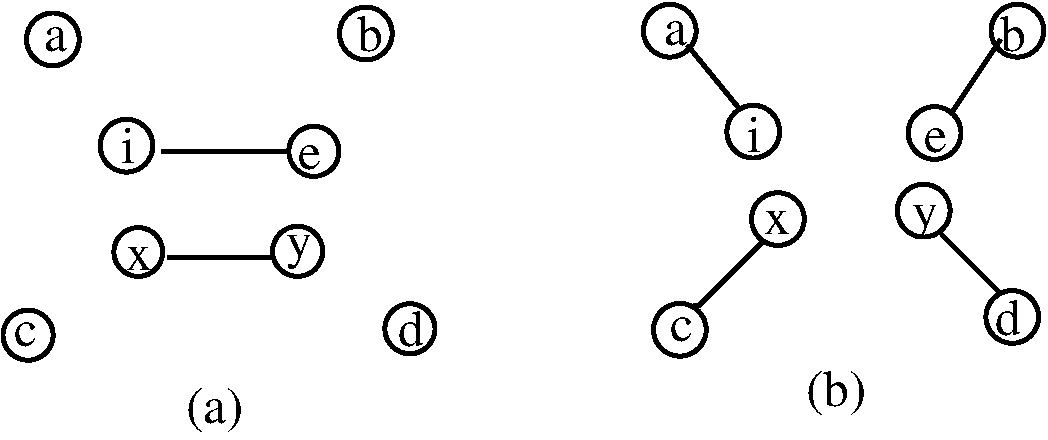
\includegraphics[width=0.7\columnwidth, angle=0]{./texfiles/Chapter_1/fig/ede_em-eps-converted-to.pdf}
 \caption{\label{fig3}(a) and (b) denote the status of the network at time $t$ and $t+1$ respectively. For the edge $(i,e)$ in $t$ the corresponding edges
 emanating from $i$ and $e$ are $(i,a)$ and $(e,b)$. For the edge $(x,y)$ they are $(x,c)$ and $(y,d)$. So the $Edge\_emer_{t}=\frac{2+2}{2}=\frac{4}{2}$}
 
%  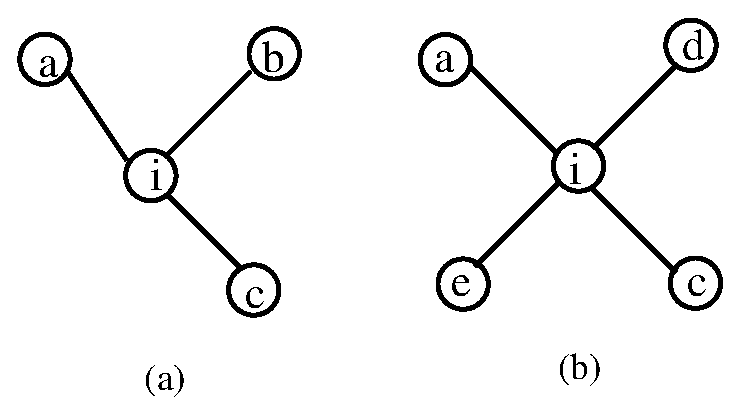
\includegraphics[width=0.8\columnwidth, angle=0]{fig/jaccard.eps}
%  \caption{\label{fig2}(a) and (b) denote the status of node $i$ at time $t$ and $t+k$ respectively. $NBR(i)_{t}=\{a,b,c\}$ and $NBR(i)_{t+k}=\{a,d,c,e\}$ 
%  $Correlation(i)_{k}$={\large$\frac{NBR(i)_{t}\bigcap NBR(i)_{t+k}}{NBR(i)_{t}\bigcup NBR(i)_{t+k}}$}={\large$\frac{2}{5}$} where $NBR(i)_{t}\rightarrow$ the set of neighbors of $i$ at time $t$}
%   
%    \includegraphics[width=0.9\columnwidth, angle=0]{fig/aging_inf2006.eps}
%  \caption{\label{aging}The value of the correlation decreases as we increase the lag between the network snapshots (INFOCOM 2006 dataset). The $X$ axis represents lag and $Y$ axis
%   represents the average correlation value.\vspace{-6mm}}
  
 
 \end{center}
 \end{figure}

   
\item (4). {\bf  Edge emergence}: Edge emergence ~\cite{sur2014attack} is a measure that estimates structural similarity. For measuring the 
  edge emergence at time $t$ we consider each edge of the network at time $t$ and for each of its two endpoints we calculate the number of edges 
  emerging in the next time step $t+1$. We represent edge-emergence at time $t$ by $Edge\_emg_{t}$. If $E_t$ denotes the set of edges present in the network at time $t$ 
  and $A_{t+1}$ denotes the set of edges at time $t+1$ which are adjacent to $E_t$ then $Edge\_emg_{t}=\frac{|A_{t+1}|}{|E_{t}|}$. 
Figure~\ref{fig3} shows how we calculate this measure for a temporal network at any time instance.
  
  
  \item (5). {\bf  Modularity}: We decompose each snapshot into communities using the technique specified in ~\cite{blondel2008fast}
  and measure the goodness of this division using modularity ~\cite{newman2006modularity}. We represent modularity 
  of the system at a given time step {$t$} by {$Mod_{t}$}. 
  
%   We also consider {\bf betweenness centrality}, {\bf closeness centrality} and {\bf clustering coefficient} and their values at time step $t$ are represented by 
%   {$Bet\_cen_{t}$}, {$Clos\_cen_{t}$} and {$Cluster\_coeff_{t}$} respectively.
  
 \end{itemize}
 We also consider (6). {\bf  betweenness centrality}, (7). {\bf closeness centrality} and (8). {\bf  clustering coefficient} of the graph (values computed for each node and then summed over all nodes) 
and their values at time step $t$ are represented by 
  {$Bet\_cen_{t}$}, {$Clos\_cen_{t}$} and {$Clus\_coeff_{t}$} respectively.

\medskip


\noindent
\section{Description of the dataset}
\label{dataset}
We perform our experiments on five human face-to-face network datasets: INFOCOM 2006 dataset~\cite{cambridge-haggle-imote-infocom2006-2009-05-29}, SIGCOMM 2009 dataset~\cite{thlab-sigcomm2009-mobiclique-proximity-2012-07-15}\footnote{http://crawdad.org/}, 
Highschool datasets (2011, 2012)~\cite{fournet2014contact} and Hospital dataset~\cite{vanhems2013estimating}\footnote{http://www.sociopatterns.org/}.


% \textcolor{blue}{The first two represent human face-to-face interaction while the last two represent 
% human interaction through social media.}
\begin{itemize}
\item {\bf INFOCOM 2006:}
This is a human face-to-face communication network and was collected at the IEEE INFOCOM 2006 conference at Barcelona.
78 researchers and students participated in the experiment. They were equipped with imotes and apart from them 20 stationary imotes were deployed as 
location anchors. The stationary imotes had more powerful battery and had a radio range of about 100 meters. The dynamic imotes had a radio range of 30 meters.
If two imotes came in each others' range and stayed for at least 20 seconds then an edge was recorded between the two imotes.
The edges were recorded at every 20 seconds. 
Therefore, this is the lowest resolution at which the experiments can be potentially conducted. However, we observe that at this resolution the network is extremely sparse 
which makes it difficult to conduct meaningful data comparison and prediction. We observe experimentally that the lowest interval that allows for appropriate comparison 
and prediction is $5$ minutes and therefore we set this value as our resolution for all further analysis.
%The network is both unweighted and undirected.
 \item {\bf SIGCOMM 2009:}
 This is also a human face-to-face communication network and was collected at the SIGCOMM 2009 conference at Barcelona, Spain. The dataset contains data collected by an opportunistic mobile social 
application, MobiClique. The application was used by 76 persons during the conference. The trace records all the nearby Bluetooth devices reported by the periodic 
Bluetooth device discoveries.
Each device performed a periodic Bluetooth device discovery every 120+/-10.24 seconds for nearby Bluetooth devices. A link was added with a device 
on discovering it. 
We remove the contacts with external Bluetooth 
devices and a network snapshot is an aggregate of data obtained for 5 minutes. 
%The network is both unweighted and undirected.

\item {\bf High school datasets:}
These are two datasets containing the temporal network of contacts between students in a high school in Marseilles taken during December 2011 and November 2012 respectively. 
Contacts were recorded at intervals of 20 seconds. We consider a network snapshot as an aggregate of data obtained for 5 minutes. 
%The network is both unweighted and undirected.

\item {\bf Hospital dataset:}
This dataset consists of the temporal network of contacts between patients and health care workers in a hospital ward in Lyon, France. Data was collected at every 20 second intervals.
 Due to sparseness of the network at 20 seconds resolution, we consider each network snapshot as an aggregated network of 5 minutes. 
 
 
 In table 1 we provide the details of the datasets.  
%  \item {\bf Twitter Hashtag co-occurrence network:}
%  This is a hashtag co-occurrence network created from the tweets posted by human users 
%  on London Olympics from 27th July 2012 to 1st August 2012 extracted from 1\% random sample.
%  The network snapshot is an aggregated network of 10 minutes each. Each node represents a unique hashtag and a link appears between 
%  two nodes if they co-occur in a tweet. The network consists of 7118 nodes i.e., unique hashtags. It is both unweighted and undirected.
%  \item{\bf Facebook posts network:}
%  \textcolor{blue}{The original network consists of a set of Facebook users (nodes) and a link appears between two users if one posts on other's wall. As it is a directed network, we need to first obtain an undirected projection of it.   
%  We divide the whole data into slots of 6 hours and a link appears in the undirected projection between two nodes if both the users have posted in each other's wall within this time window. 
%  Thus we obtain an undirected projection of the original directed network and we perform our analysis on this network. Note that due to this conversion we found several 
%  such 6 hour slots without any edge making the series discontinuous.
%  All our further analysis is on the part of the whole window where we have continuous datapoints for the longest stretch.
%  %We take out only that part of the whole time window with a large sequence of consecutive 
%  %slots. Thus the final network stretches for this time window only.
%  The network consists of 20284 unique users.}
%  
 \end{itemize}
 
\begin{table*}
\centering
\begin{adjustbox}{max width=\textwidth}
\begin{tabular}{|c|c|c|c|c|c|}
\hline
Dataset         & \# unique nodes & \# unique edges & edge type  & \begin{tabular}[c]{@{}l@{}}Time span of \\ the dataset\end{tabular}     & \begin{tabular}[c]{@{}l@{}}Time steps \\ for  prediction\end{tabular} \\ \hline
INFOCOM 2006    & 98              & 4414            & undirected &  1120                                                                   & 200 - 800                                                             \\ \hline
SIGCOMM 2009    & 76              & 2082            & do         &  1068                                                                   & 300 - 900                                                             \\ \hline
Highschool 2011 & 126             & 5758            & do         &  1215                                                                   & 200 - 900                                                           \\ \hline
Highschool 2012 & 180             & 8384            & do         &  1512                                                                   & 200 - 1000                                                            \\ \hline
Hospital        & 75              & 5704            & do         &  1158                                                                   & 100 - 900                                                             \\ \hline
\end{tabular}
\end{adjustbox}
\label{tab_data}
\caption{Properties of the dataset used.}
\end{table*}
\medskip


\noindent
\section{Analysis of time series}
\label{properties}

We now present the plots of the time series and analyze their properties based on both time domain and frequency domain characteristics. 
%{\bf tell what you observe from the time series and how you are able to differentiate between the two types of temporal network}
%We plot the time series for some of the properties in figure~\ref{fig4}, figure~\ref{fig5}, figure~\ref{twitter} and figure~\ref{fb_post} for INFOCOM 2006, SIGCOMM 2009, Twitter hashtag co-occurrence and Facebook posts datasets respectively.
\begin{figure*}[!ht]
  \centering
  \includegraphics*[width=0.9\textwidth,angle=0]{./texfiles/Chapter_1/fig/infocom_all-eps-converted-to.pdf}
% \includegraphics*[width=0.3\textwidth,height=30mm,angle=0]{fig/clus_coeff.eps}	
% \includegraphics*[width=0.3\textwidth,height=30mm,angle=0]{fig/avg_deg.eps}
  
%  \hspace{6mm}(a)\hspace{52mm}(b)\hspace{52mm}(c)
  
 %\caption{\label{fig4}Time series plotsfor the properties}
  
  
  \centering
  \includegraphics*[width=0.9\textwidth,angle=0]{./texfiles/Chapter_1/fig/sigcomm_all-eps-converted-to.pdf}
  
  \centering
  \includegraphics*[width=0.95\textwidth,angle=0]{./texfiles/Chapter_1/fig/highschool_2011_psd-eps-converted-to.pdf}
  %\centering
  %\includegraphics*[width=0.95\textwidth,angle=0]{fig/highschool_2011_psd.eps}
  
  
%   \centering
%   \includegraphics*[width=0.95\textwidth,angle=0]{fig/highschool_psd.eps}
  
%   \centering
%   \includegraphics*[width=0.95\textwidth,angle=0]{fig/hospital_psd.eps}
% \includegraphics*[width=0.3\textwidth,height=30mm,angle=0]{fig/avg_deg_plot_sigcomm.eps}	
% \includegraphics*[width=0.3\textwidth,height=30mm,angle=0]{fig/clus_coeff_plot_sigcomm.eps}
  
%  \hspace{6mm}(a)\hspace{52mm}(b)\hspace{52mm}(c)
  
%   \caption{\label{fig5}Time series plots for SIGCOMM 2009 dataset. (a) Number of active nodes (b) Average degree (c) Clustering coefficient. The plots are 
%  the values of these measurements at time corresponding to the values in the X-axis}
  
%  \centering
%  \includegraphics*[width=0.95\textwidth,angle=0]{fig/Twitter_all.eps}
% \includegraphics*[width=0.3\textwidth,height=30mm,angle=0]{fig/avg_deg_twitter.eps}	
% \includegraphics*[width=0.3\textwidth,height=30mm,angle=0]{fig/clo_cen_twitter.eps}
  
%  \hspace{6mm}(a)\hspace{52mm}(b)\hspace{52mm}(c)
  
 % \caption{\label{twitter}Time series plots for Twitter Hashtag co-occurrence during London olympics 2012. (a) Number of active edges, (b) Average degree, (c) Closeness centrality. The plots are 
 % the values of these measurements at time corresponding to values in the X-axis}

  % \centering
  %\includegraphics*[width=0.95\textwidth,height=30mm,angle=0]{fig/facebook_all.eps}
 %\includegraphics*[width=0.3\textwidth,height=30mm,angle=0]{fig/avg_deg_fb.eps}	
 %\includegraphics*[width=0.3\textwidth,height=30mm,angle=0]{fig/clo_cen_fb.eps}
  
 % \hspace{6mm}(a)\hspace{52mm}(b)\hspace{52mm}(c)
  
  %\caption{\label{fb_post}{\bf NEED TO CHANGE}}
   \caption{\label{fig_all_dataset} (A), (C) and (E) represent the time series plots for INFOCOM 2006, SIGCOMM 2009 and High-school 2011 respectively. (B), (D) and (F) represent the power spectral density (PSD) corresponding to the frequency bins for INFOCOM 2006, SIGCOMM 2009 and High-school 2011 dataset respectively. Bins 1, 2 and 3 corresponds to frequencies $<$5, 5-15 and $>$15(Hz) respectively.}
%   
 \end{figure*}
  %From the time series plots we can make the following observations about the key properties:
  \begin{figure*}[!ht]
%   \centering
%   \includegraphics*[width=0.95\textwidth,angle=0]{fig/highschool_psd.eps}
  
    \centering
  \includegraphics*[width=0.95\textwidth,angle=0]{./texfiles/Chapter_1/fig/highschool_psd-eps-converted-to.pdf}
  
  \centering
  \includegraphics*[width=0.95\textwidth,angle=0]{./texfiles/Chapter_1/fig/hospital_psd-eps-converted-to.pdf}
  
  \caption{\label{fig_all_dataset_1} (A) and (C) represent the time series plots for High-school 2012, Hospital respectively. (B) and (D) represent the power spectral density (PSD) corresponding to the frequency bins for High-school 2012 and Hospital dataset respectively. Bins 1, 2 and 3 corresponds to frequencies $<$5, 5-15 and $>$15(Hz) respectively.}
  
  \end{figure*}
 % \begin{figure*}[!ht]
  %\centering
  %\includegraphics*[width=0.95\textwidth,angle=0]{fig/facebook_all.eps}
%  \includegraphics*[width=0.3\textwidth,height=35mm,angle=0]{fig/acf_inf06_bcen.eps}	
%  \includegraphics*[width=0.3\textwidth,height=35mm,angle=0]{fig/acf_inf06_clus_coeff.eps}
% 
%  \hspace{6mm}(a)\hspace{52mm}(b)\hspace{52mm}(c)
%  
%  \caption{\label{fig6} Auto-correlation plots for INFOCOM 2006 dataset. (a) Average degree, (b) Betweenness centrality, (c) Clustering coefficient. The correlation value is 
%  represented by Y-axis and lag is represented by X-axis.}
%  
%  \includegraphics*[width=0.3\textwidth,height=35mm,angle=0]{fig/acf_sig_act_edge.eps}
%  \includegraphics*[width=0.3\textwidth,height=35mm,angle=0]{fig/acf_sig_avg_deg.eps}	
%  \includegraphics*[width=0.3\textwidth,height=35mm,angle=0]{fig/acf_sig_mod.eps}
% 
%  \hspace{6mm}(a)\hspace{52mm}(b)\hspace{52mm}(c)
%  
%  \caption{\label{fig7} Auto-correlation plots for SIGCOMM 2009 dataset. (a) Number of active edges, (b) Average degree, (c) Modularity. The correlation value is 
%  represented by Y-axis and lag is represented by X-axis.}
%  
%  \centering
%   \includegraphics*[width=0.3\textwidth,height=30mm,angle=0]{fig/acf_twit_act_nodes.eps}
%  \includegraphics*[width=0.3\textwidth,height=30mm,angle=0]{fig/acf_twit_clo_cen.eps}	
%  \includegraphics*[width=0.3\textwidth,height=30mm,angle=0]{fig/acf_twit_avg_clus.eps}
%   
%   \hspace{6mm}(d)\hspace{52mm}(e)\hspace{52mm}(f)
%   
%   \caption{\label{twitter_acf}Auto-correlation plots for Twitter Hashtag co-occurrence dataset. (a) Number of active nodes, (b) Closeness centrality, (c) Clustering coefficient. 
%   The correlation value is 
%  represented by Y-axis and lag is represented by X-axis.}
%  
%  \centering
%   \includegraphics*[width=0.3\textwidth,height=30mm,angle=0]{fig/node_fb_acf.eps}
%  \includegraphics*[width=0.3\textwidth,height=30mm,angle=0]{fig/clo_cen_fb_acf.eps}	
%  \includegraphics*[width=0.3\textwidth,height=30mm,angle=0]{fig/avg_deg_fb_acf.eps}
%   
%   \hspace{6mm}(d)\hspace{52mm}(e)\hspace{52mm}(f)
  
%   \caption{\label{fig_all_dataset} (A),(C),(E) and (G) represent the time series plots for INFOCOM 2006, SIGCOMM 2009, Twitter hashtag and 
%   Facebook post dataset respectively. (B),(D),(F) and (H) represent the power spectral density (PSD) corresponding to the frequency bins for INFOCOM 2006, SIGCOMM 2009, Twitter hashtag and 
%   Facebook post dataset respectively. Bins 1,2 and 3 corresponds to $<$5, 5-15 and $>$15(Hz) respectively.}
 
%\end{figure*}

\subsection{Time domain characteristics}

For the time domain analysis of the properties we look into the time series plots for the datasets represented in figures ~\ref{fig_all_dataset}(A), (C), (E) and 
~\ref{fig_all_dataset_1}(A), (C).
From the time series plots we observe the presence of periodicity in almost all the datasets. A stretch of high values is followed by a stretch of low values 
and so on. However, they are of varying lengths.  
% If we compare the time-series plots in figures ~\ref{fig_all_dataset}(A) and (C) (human face-to-face communication networks) with the time series 
% plots in figures ~\ref{fig_all_dataset}(E) and (G) (human communication through social media), we observe that while for the 
% former case a periodic pattern is
% present, no such pattern is present for the latter case. 
This indicates the presence of correlation in case of human face-to-face communication network.
We quantify this structural correlation later in this paper. 
%We also do not observe any measurable trend in any of the four datasets since none 
%of them seem to be globally increasing, decreasing or keeping constant with time. 
We also check whether these time series are stationary. 
On performing KPSS (Kwiatkowski–Phillips–Schmidt–Shin) ~\cite{kwiatkowski1992testing} and 
 ADF (Augmented Dickey Fuller) test ~\cite{dickey1979distribution} on the data we conclude that the data is non-stationary. 
 Overall, the presence of correlation in case of human face-to-face network indicates that it is a stochastic process with memory i.e., the contacts a node 
 makes in the current time step is influenced by its contact history. 
%  The network of human contact through social media is memory-less i.e., the 
%  network at each time step is random.
% % For the time series plots of the human face-to-face contact network (INFOCOM 2006 and SIGCOMM 2009), we observe that periodicity appears to be present in the 
%  time series with a stretch of high values followed by another stretch of low values and so on. But these periods are inconsistent. Another 
%  important observation that we make from these plots is that the 
%    \begin{itemize}
%  \item {\bf Periodicity:}figures 
%  Periodicity represents the repetition of data in a time series at certain time intervals. 
%  In case of INFOCOM 2006 and SIGCOMM 2009 datasets as shown in figures ~\ref{fig4} and ~\ref{fig5} respectively, periodicity appears to be present in the 
%  time series with a stretch of high values followed by another stretch of low values and so on. But these periods are inconsistent. For Twitter hashtag co-occurrence and Facebook posts network  
%   as shown in figure ~\ref{twitter} and ~\ref{fb_post} respectively, periodicity is not present.
%  \item {\bf Trend:}
%  Trend represents the global nature of a time series indicating whether the series is gradually increasing, decreasing or remaining constant with time.  
%  There is also no measurable consistent  trend in the data as the series do not appear to increase or decrease with time in case of INFOCOM 2006 and SIGCOMM 2009 datasets. 
%  For the Facebook data one observes a slightly increasing trend in the number of active nodes.
%  \item {\bf Seasonality:}
%  Seasonality represents the specific patterns in a time series occurring at certain time steps and is identified by comparing two similar time series: for instance, 
% the temperature recorded over the months for two or more years shows that it tends to increase during the summer months and decreases during winter.    
%  Seasonality may also be present in our case as well but it cannot 
%  be checked as we have no other similar series to compare with. 
% 
% \end{itemize}
 
%  For a more quantitative analysis we further look into the auto-correlation (ACF) plots of the time series. The auto-correlation $r$ at a lag $k$ is given by the formula-
%  \begin{center}
%  {\large $r_k=\frac{\Sigma_{t=1}^{N-k}(x_t-\mu)(x_{t+k}-\mu)}{\Sigma_{1}^{N}(x_t-\mu)^{2}}$}
%  \end{center}
% where $\mu$ is the mean and $x_t$ is the value at time $t$. Figures ~\ref{fig6} and ~\ref{fig7} represent the auto-correlation plots for INFOCOM 2006 and 
% SIGCOMM 2009 datasets respectively.
% The correlation value is 1 at lag 0 and it gradually decreases with increasing lag. Clearly it represents a stochastic 
% process that is not random since, for a random process the correlation value is 1 at lag 0 and negligible for the rest. As is evident from the plots, the time 
% series is also not alternating. The ACF plots also show indications of periodicity as it can be observed from the time series plots. 
% Initially, it shows a decreasing trend with the value gradually going to zero. The series then continues its decreasing trend reaching negative values; 
% after a point, it again starts increasing. It then reaches zero and continues its upward trend and so on.   
% One can also observe that the correlation value decreases gradually and does not get to zero until a large value of the lag. 
% Thus the series appears to be non-stationary. We further performed two tests- KPSS (Kwiatkowski–Phillips–Schmidt–Shin) ~\cite{kwiatkowski1992testing} and 
% ADF (Augmented Dickey Fuller) test ~\cite{dickey1979distribution} on the data and concluded that the process is indeed non-stationary.  
% In case of the hashtag co-occurrence network we observe that the time series representing the properties differ in their characteristics. In fact, we observe that 
% they can be sub-divided into two sets with one showing short term correlations and evidence of non-stationarity while the other is completely random. 
% Figure ~\ref{twitter_acf} represents the auto-correlation function plots for Twitter hashtag co-occurrence during London Olympics 2012 event.
% This is in contrast to the previous cases where all the time series were of similar nature.
% \textcolor{blue}{In case of Facebook posts network we observe the time series plot to be alternating between positive and negative and decaying to 0 only very slowly 
% for some of the properties while for others it is random like in case of Twitter (figure~\ref{fb_post_acf}).
% %We thus conclude that a growth model which successfully mimics human mobility dynamics may not be able to mimic other temporal networks and hence a single growth model 
% %is not sufficient to explain all temporal networks.
% So these networks represent a process which is mostly markovian in nature i.e., the network at each time step has almost no structural dependence on the 
% network at previous time steps. 
% We thus conclude that a single growth model might not be suitable to reproduce the strikingly different physical properties of these classes of 
% temporal networks. In general, a systematic approach would be to have a different growth model for every single such class.}
 


\medskip

 
\noindent
\subsection{Frequency domain analysis}
\label{spectrogram}
 


We perform the frequency domain analysis of 
the time series extracted from the temporal network
%We can convert a time series from its time domain to its frequency domain using Discrete Fourier Transform (DFT). However, instead of taking the discrete fourier transform of the whole series we 
by conducting
  a spectrogram analysis of the data. Spectrogram analysis is a short time fourier transform 
where we divide the whole time series into several equal sized windows and apply discrete fourier transform on this widowed data.
The main advantages of using spectrogram analysis are
 (a). we do not lose the time information,
 (b). we are able to obtain a view of the local frequency spectrum.
Also note that the spectrogram analysis allows us to identify as well as quantify the fluctuations in the data which is difficult to identify 
from the corresponding time series. 
A high concentration of low frequency components would indicate lower fluctuations in the data; in contrast no such concentration of low frequency components 
would indicate higher fluctuations and irregularities in the data.
%These fluctuations have a direct relation to our prediction framework as lower the fluctuations in data higher is the prediction accuracy and vice versa.

We construct the spectrogram and segregate the power spectral density (PSD measured in Watts/Hz) based on the frequency into three bins. In bin 1 we calculate the mean PSD 
corresponding to the frequencies $<$ 5 Hz, in bin 2 we calculate the PSD corresponding to frequencies between 5 and 15 Hz and bin 3 consists of the 
mean PSD value corresponding to frequencies $>$ 15 Hz. We call them LPSD, MPSD and HPSD respectively.
So a higher value of mean PSD corresponding to bin 1 (LPSD) would indicate lower fluctuations in data. 
In figures ~\ref{fig_all_dataset}(B), (D), (E) and ~\ref{fig_all_dataset_1}(B), (D) we plot the PSD corresponding to the three bins across all the properties for all the datasets. We 
observe that the lower frequencies dominate to a higher extent in case of the properties like number of active nodes, number of active edges, modularity 
but to a much lower extent in case of betweenness centrality, closeness centrality and clustering coefficient.  
In fact the prediction accuracy of a property can be enhanced through spectrogram analysis.
%this could be a good indicator of prediction accuracy of a property.
% But for the human face-to-face networks the PSD values 
% are much higher than in case networks of human contact through social media. This indicates that the time series corresponding to human face-to-face 
% network are more consistent and hence correlated than the network representing human contact through social media.



% Thus both the time domain analysis and the frquency domain analysis indicate that the evolution dynamics of human contact network through physical proximity (face-to-face) 
% and through social media differ significantly and it is almost impossible to obtain a generic growth model for these networks.
% In figure~\ref{fig10} we plot the spectrograms for number of active nodes and betweenness centrality for both INFOCOM 2006 and SIGCOMM 2009 datasets.
% Spectrogram analysis also requires the size of the series to be in the power of 2 or else it pads the rest of the time points until the closest power of 2
% with zeros. Therefore, we select 1024 time steps from 51 to 1074 in case of INFOCOM 2006 dataset and 43 to 1067 in case of SIGCOMM 2009 dataset.
% 
% Since we are not losing the time information as well as getting the local information, we use spectrograms in two ways-
% \begin{itemize}
%  \item From the spectrogram of the whole series we can determine whether this property of the network can be predicted with minimum error.
%  \item Using the local information we can determine whether a prediction at a certain time point would be erroneous or not before applying our prediction technique.
% \end{itemize}

% We have previously seen that for the property number of active nodes, we get the best prediction results and for betweenness centrality we obtain worse results.
% Here we check whether we can distinguish these two properties using the spectrogram of the whole time series. 
% In the figure ~\ref{fig10}(a) (spectrogram for number of active nodes), we find that throughout all the windows the frequency spectrum 
% is highly dominated by the low frequencies within range 0-3 Hz. In contrast if we look at the figure of 13(b) (spectrogram for betweenness centrality), we find a 
% very different behavior. In most of the windows the frequency spectrum consists of a number of frequencies and from the color bar it can be seen that 
% none of them dominates. These observations also hold for the other properties as well. Thus, we may conclude that the spectrogram response determines
% the goodness of our prediction. 
% If the frequency spectrum is distributed we conclude that the prediction may not be accurate for this time step. While if the 
% spectrogram is concentrated only to a small range of low frequencies, the predictions should be far better.
% 
% We now outline how to use spectrograms to make our predictions better. When predicting the value at any time step, before applying the prediction technique 
% we plot the spectrogram of the previous 128 time points. By analyzing this spectrogram, we determine whether our framework, on application would provide 
% significantly accurate predictions. For our analysis we considered the respective spectrograms for low prediction error time points and high prediction error 
% time points. 
% 
% 
%  In figure ~\ref{fig11} we show spectrograms of two such time points: one with prediction error around 1\% and the other with a prediction error of 98\%. 
%  It can be observed that in the former case the frequency spectrum is dominated with low frequencies while the other frequencies have negligible influence 
%  on the spectrogram. On the other hand for the latter case the spectrum is influenced by a large set of frequencies although very loosely. 
%  Note that these results are representative and 
%  similar observations were encountered for other points as well. Thus while predicting the value of the series at any time point we conduct a spectrogram  
%  analysis and conclude whether our framework would produce significantly accurate results.


\medskip


\noindent

 \section{Prediction framework}
 \label{prediction}
 

\begin{figure}
 \begin{center}
 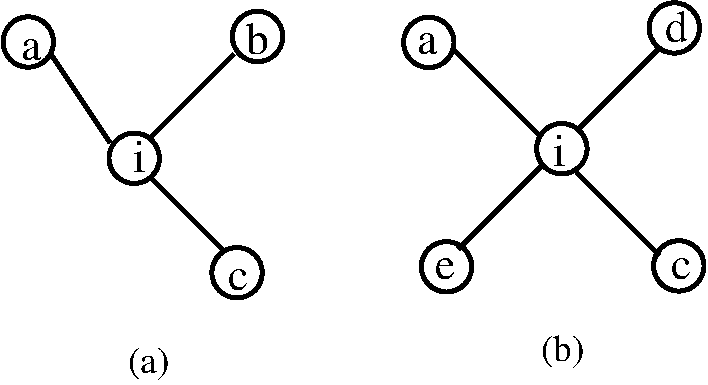
\includegraphics[width=0.45\columnwidth, angle=0]{./texfiles/Chapter_1/fig/jaccard-eps-converted-to.pdf}
 \caption{\label{fig2}(a) and (b) denote the status of node $i$ at time $t$ and $t+k$ respectively. $NBR(i)_{t}=\{a,b,c\}$ and $NBR(i)_{t+k}=\{a,d,c,e\}$ 
 $Correlation(i)_{k}$={\large$\frac{NBR(i)_{t}\bigcap NBR(i)_{t+k}}{NBR(i)_{t}\bigcup NBR(i)_{t+k}}$}={\large$\frac{2}{5}$} where $NBR(i)_{t}\rightarrow$ the set of neighbors of $i$ at time $t$}
  \end{center}
 \end{figure}
  
 \begin{figure*}
 \centering
   \includegraphics*[width=0.75\textwidth,angle=0]{./texfiles/Chapter_1/fig/age_all_5-eps-converted-to.pdf}
%    \hspace{20mm}(A)\hspace{20mm}(B)\hspace{20mm}(C)\hspace{20mm}(D)\hspace{20mm}(E)
 \caption{\label{aging}The average neighborhood-overlap value at different lags for (A)INFOCOM 2006, (B)SIGCOMM 2009, (C)Highschool 2012, (D)Highschool 2011 and (E)Hospital datasets.}
%\end{center}
 \end{figure*}

%  \begin{figure}
%  \begin{center}
%   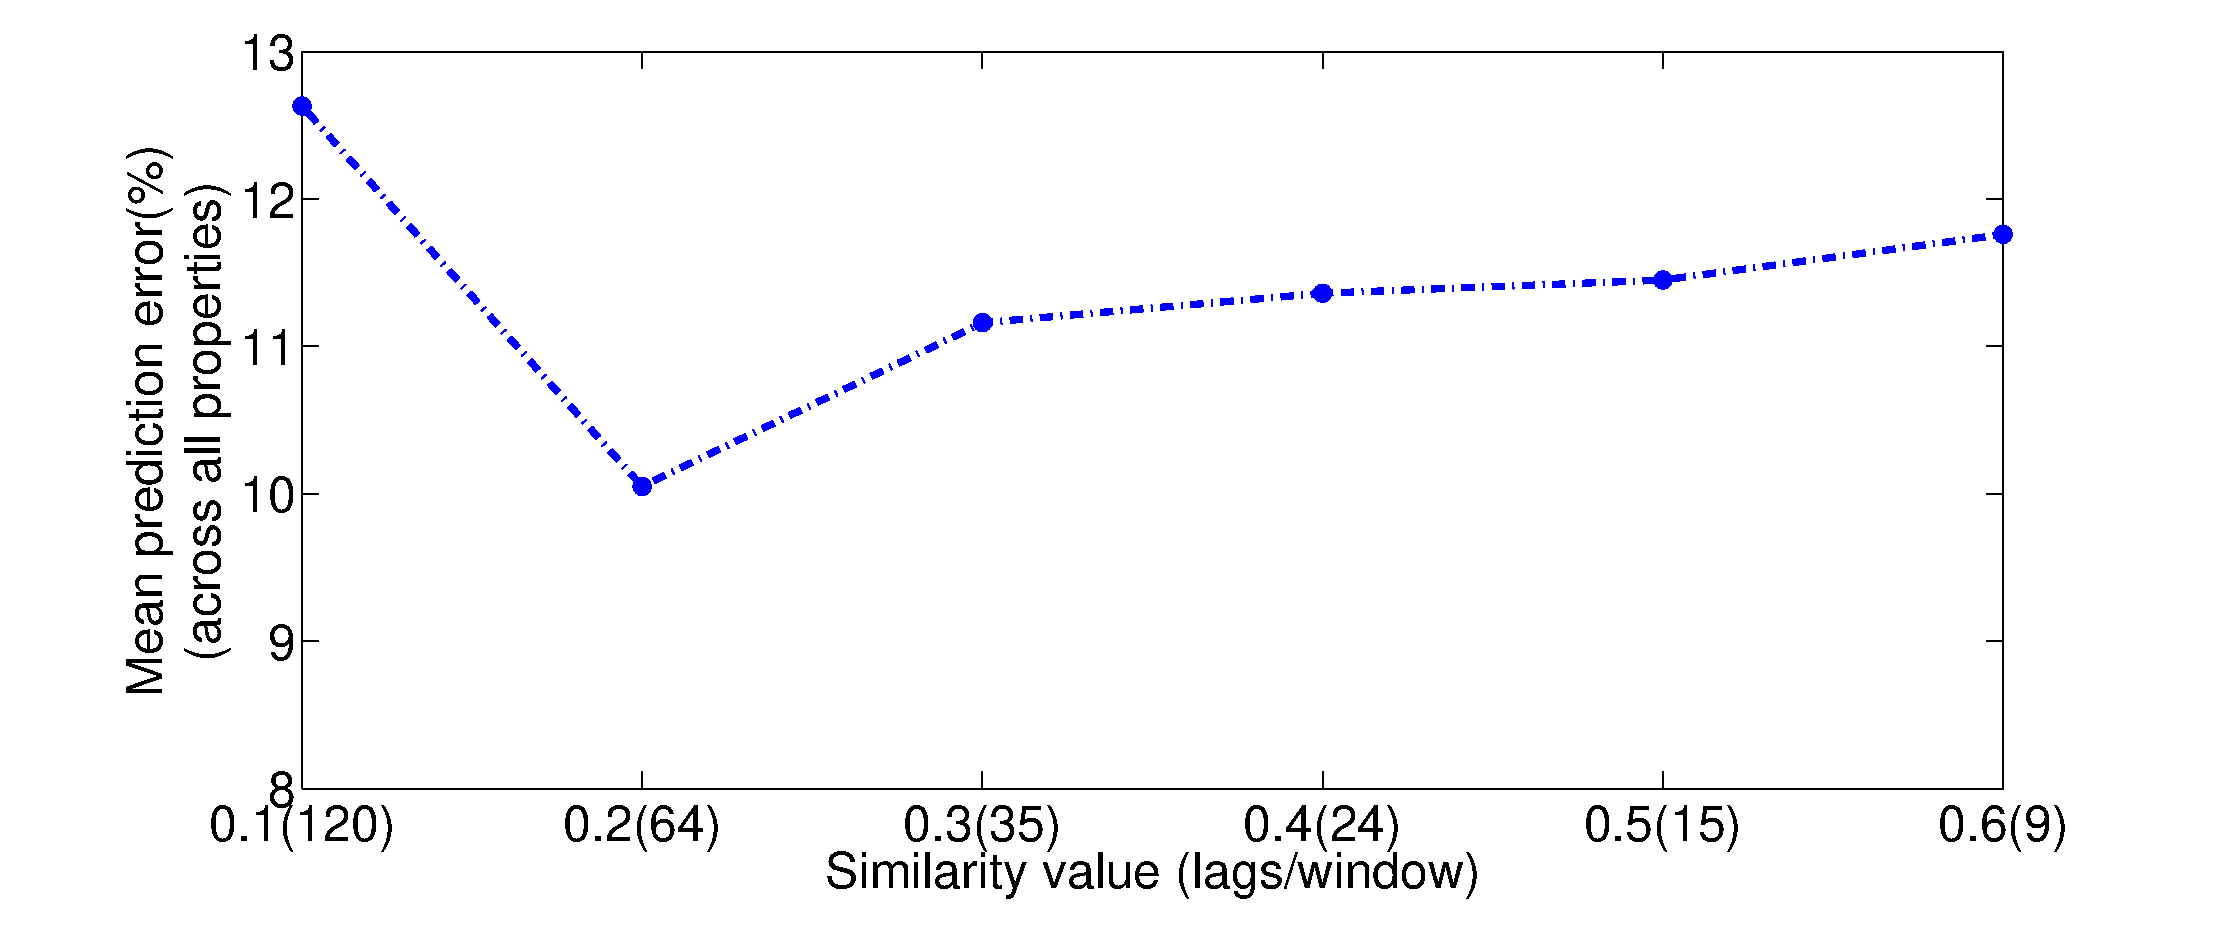
\includegraphics[width=0.75\columnwidth, angle=0]{fig/error_similarity_val.eps}
%   \caption{\label{fig_err} Mean prediction error (\%) across different properties for INFOCOM 2006 dataset for different similarity values. The lags corresponding to the similarity 
%   value are also provided.}
%   \end{center}
%  \end{figure}




% \begin{figure*}
%   \centering
%   \includegraphics*[width=0.95\textwidth,angle=0]{fig/error_dist_all.eps}
%  
%  %\hspace{8mm}(a)\hspace{60mm}(b)
%  
%  \caption{\label{fig8}  The percentage error distribution of all the properties (time series) for (A) INFOCOM 2006 dataset, (B) SIGCOMM 2009 dataset, (C) High-school 2011. (D) High-school 2012 and (E) Hospital. 
%  X-axis represents percentage error and Y-axis represents 
%  probability.}
% \end{figure*} 
  
In this section, we employ the time series to forecast the different structural properties of the temporal networks.
%Note that this process is equivalent to having a growth model for the temporal networks.
Elementary models of time series forecasting could be categorized into Auto-regressive(AR) and Moving average(MA) models ~\cite{chatfield2013analysis}. In case of 
an auto-regressive model of order $p$, AR($p$), the value of the time series at time step $t$ is given as - 
\begin{center}
 $y_{t}=\alpha_{1}y_{t-1}+\cdots+\alpha_{p}y_{t-p}+e_t+c$
\end{center}
where $\alpha_{i}$s are parameters, $e_t$ is the white noise error term and $c$ is a constant.
Similarly, in case of Moving average model of order $q$, MA($q$), the value of the time series at time step $t$ is given as - 
\begin{center}
 $y_{t}=\beta_{1}e_{t-1}+\cdots+\beta_{q}e_{t-q}+\mu+e_t+c$
\end{center}
where $\beta_{i}$s are parameters, $e_t,e_{t-1},...$ are white noise error terms and $\mu$ is the expectation of $y_t$.
These two models could be combined into Auto-regressive-moving-average (ARMA($p$,$q$)) ~\cite{chatfield2013analysis} where the value of the time series at time step $t$ is given as
\begin{center}
 $y_{t}=\alpha_{1}y_{t-1}+\cdots+\alpha_{p}y_{t-p}+\beta_{1}e_{t-1}+\cdots+\beta_{q}e_{t-q}+e_t+c$
\end{center}

However, in our case the time series show evidences of non-stationarity and short term dependencies and these models are insufficient and hence we use ARIMA model ~\cite{box2011time} for forecasting. The initial differncing step in ARIMA model 
is used to reduce the non-stationarity.
%Any ARIMA model has three parameters $p$, $d$ and $q$. $p$ is the auto-regressive element representing the lingering effects of preceding scores.
%$d$ represents the integrated element and $q$ represents the moving average element.
On fitting an ARIMA($p$,$d$,$q$) model to a time series we obtain an auto-regressive 
equation of the form-

\begin{center}
 $y_{t}=\alpha_{1}y_{t-1}+\cdots+\alpha_{p}y_{t-p}+\beta_{1}e_{t-1}+\cdots+\beta_{q}e_{t-q}+c$
\end{center}


Hence we can take a time series corresponding to a network property and fit an ARIMA model to it. Thus, we obtain an auto-regressive equation for that series which 
can be used 
in forecasting. 
% Note that our forecast results are performed on INFOCOM 2006 and SIGCOMM 2009 datasets. 
% For the Twitter hashtag co-occurrence dataset we find the time series corresponding to only some of the properties that are observed to possess a short term correlation.
% We perform our predictions only for these properties.
% For Facebook posts network also we do not perform any predictions as we find only two of the properties to be suitable for prediction. 
In order to predict a value at a future time point, we divide the data in smaller parts and perform our predictions on these smaller stretches.
In the next subsection we discuss how we perform this division.

\subsection{Selecting a window}

In order to identify the right length of a stretch (i.e., a window size) we need to identify how the network at any time point is influenced by the network at the previous time points.
The basic idea is that the time points to which this influence extends should all get included into a single window.
To quantify this influence we define a new metric called {\bf neighborhood-overlap} which measures the structural correlation between network snapshots at 
two time steps. We define the difference between these two time steps as the lag. To measure the neighborhood-overlap of the network snapshots at time 
$t$ and $t+k$, we calculate for each active node at time $t$ the overlap in its neighborhood between two time points. 
To measure this overlap we use the 
  standard Jaccard similarity as has been pointed out in ~\cite{TSMML10:smallworld}. Note that this is one of the most standard and interpretable ways to 
  measure structural similarity as has been identified in the literature with applications ranging from measuring keyword similarity ~\cite{niwattanakul2013using} to 
  similarity search in locality-sensitive-hashing (LSH) ~\cite{bawa2005lsh}. It has also been extensively used in link prediction ~\cite{lu2011link,lu2009similarity} 
  as well as community detection ~\cite{pan2010detecting}.
%\todo{Please give reference from Physics paper - prefereably EPJB}
Figure~\ref{fig2} shows how we formulate this measure using the Jaccard similarity index. We represent the neighborhood overlap at lag $k$ as the mean value 
  across all the active nodes in time step $t$. 
  To measure the extent of similarity we measure neighborhood-overlap for each snapshot at different lags and take the average of them. This essentially 
  shows, given a time specific snapshot how the similarity changes as we increase the lag. Figures ~\ref{aging}(A) - (E) show how this similarity 
  changes with time as we increase lag for the five different datasets. 
  As we increase the lag the similarity  
 decreases almost exponentially and hence considering snapshots at larger lag where the similarity value is very low could introduce error in learning the auto-regressive equation. 
 Also for a higher similarity value the corresponding lag would increasingly introduce more error in the fit due to lesser number of data points on which the ARIMA model gets trained
 to learn the fit function (see figure ~\ref{fig_err}).
 In fact we observed that the error in prediction increases if we consider a lag too small (high similarity value) or too large (low similarity value) (see figure ~\ref{fig_err}). 
 Hence we consider the similarity value of $0.2$ as the threshold for calculating the lag. For our prediction framework the corresponding value of the lag acts as 
 the window for fitting the ARIMA model.
  
  Let the size of the window be $w$ and we want to predict the value of the time series at time $t$. To our aim we consider the time series of the previous $w$ 
  time steps consisting of the values between time steps $t-1-w$ to $t-1$ and fit the ARIMA model to it and obtain its value at time step $t$. 
 We repeat this procedure for forecasting at every value of $t$. Thus, the time step $t$ is the test point and the series of points $t-w-1$ to $t-1$ form the 
  training set. One can imagine this process as a sliding window of size $w$ which is used for learning the auto-regressive equation and the point that falls immediately 
  outside the window is the unknown that is to be predicted.
  
  \begin{figure}
 \begin{center}
  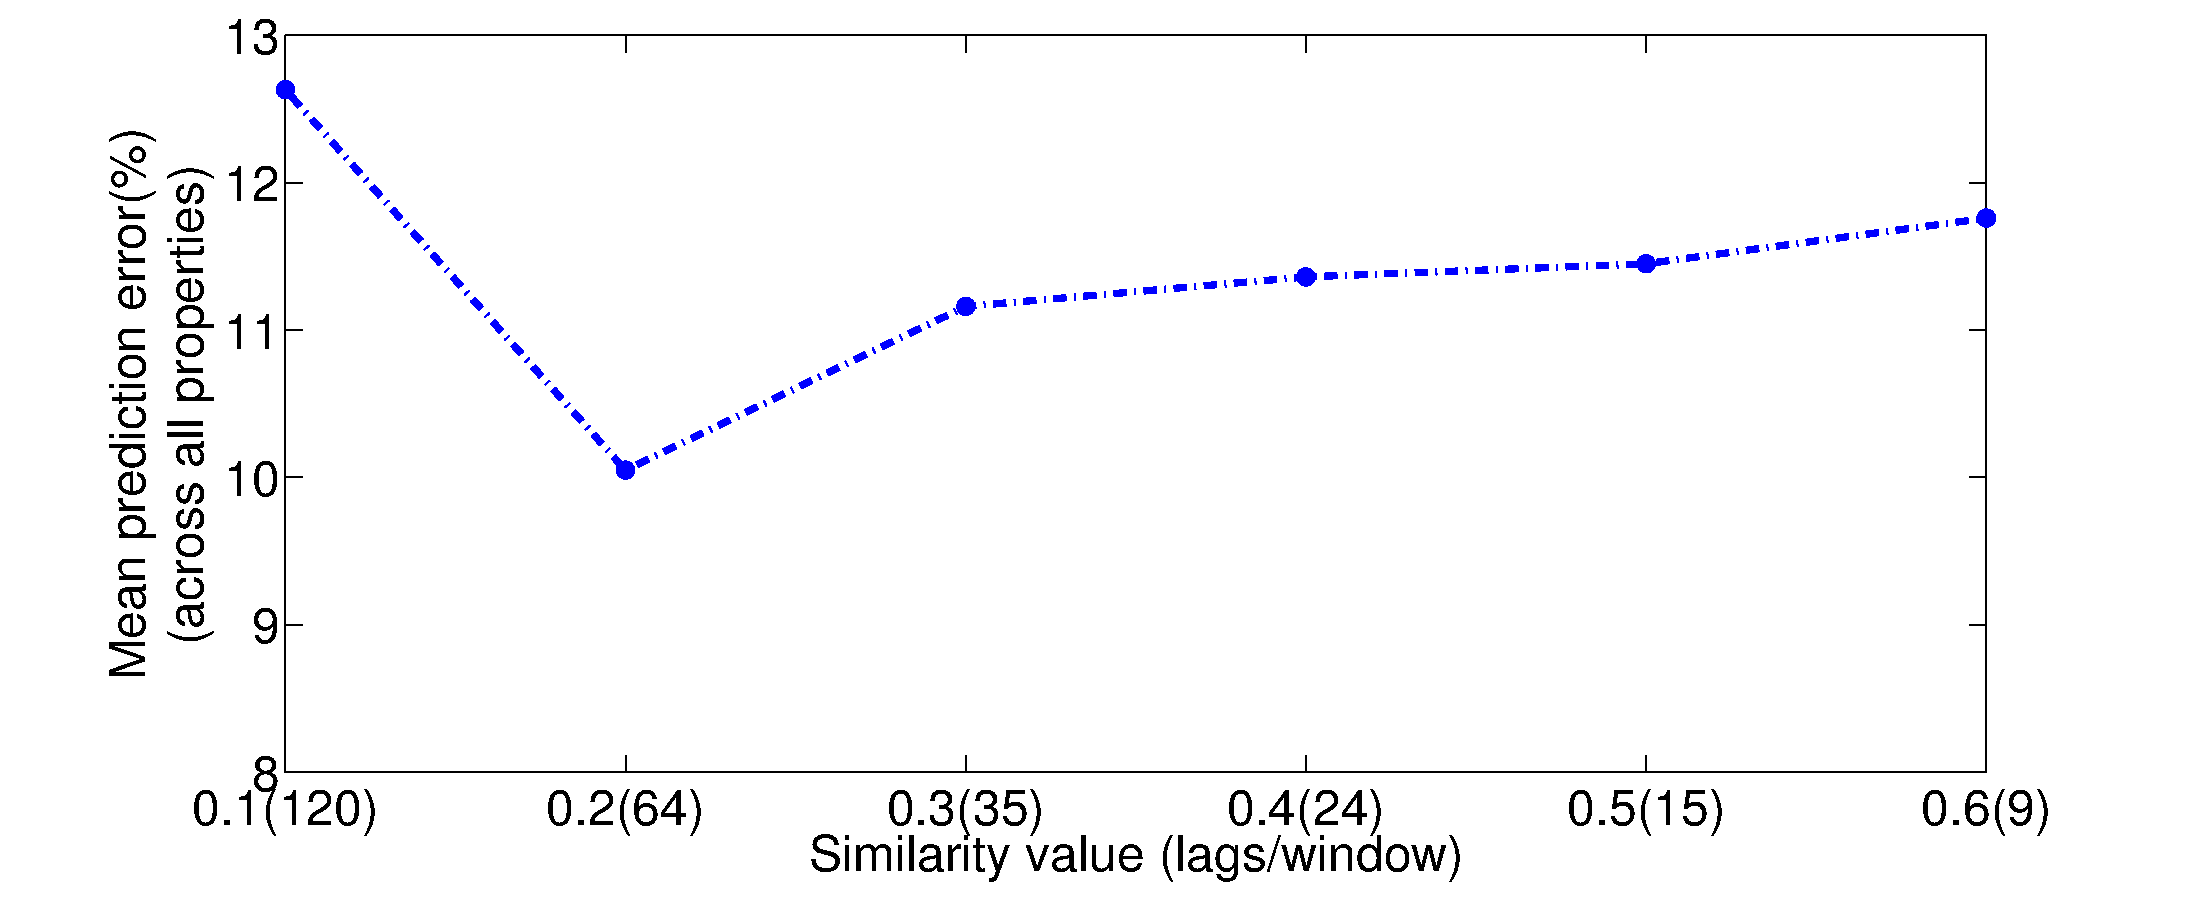
\includegraphics[width=0.75\columnwidth, angle=0]{./texfiles/Chapter_1/fig/error_similarity_val-eps-converted-to.pdf}
  \caption{\label{fig_err} Mean prediction error (\%) across different properties for INFOCOM 2006 dataset for different similarity values. The lags corresponding to the similarity 
  value are also provided.}
  \end{center}
 \end{figure}
  
  
  %   Figure ~\ref{aging} gives the value of the measure at different lags for INFOCOM 2006 dataset. To calculate the correlation value at a certain lag, we take each network snapshot 
%   and measure the average neighborhood-overlap with the snapshot at that lag and take the mean of the values.
% We observe that the value of the structural correlation decreases as we increase the lag. The correlation drops to less than 
% $0.2$ at lag around $70$.
%Therefore we select a window of size 64. 
%We could have selected any other value between 60 and 70, but we select 64 as it is in the power of 2 and it helps in the spectrogram 
%analysis we do later. 
% We observe that any choice of window size between 50 and 70 only negligibly affects the prediction outcomes. However, we set the window size to 64 since this is the 
% only poer of 2 in this admissible range and the spectrogram analysis requires that the window size to be a power of 2.
% For prediction purposes we feed the ARIMA model with the previous 64 values of the time series in order to obtain the value 
% of the current time point. 
% For the SIGCOMM 2009 dataset we perform a similar analysis and obtain a window of size 100. As it is not in the power of 2, we use a window of size 128 
% (closest integer to 100 with power of 2) for the corresponding spectrogram analysis. For the Twitter dataset we find the structural correlation to be very low 
% and it reduces even further as we increase the lag. We consider only a very small window of size 24. We do not perform spectrogram analysis for this dataset.}
% \subsection{Enhancing the prediction scheme through spectrograms}
% 
% We use spectrograms in two ways-
%  \begin{itemize}
%   \item From the spectrogram of the whole series we can determine whether this property of the network can be predicted with minimum error.
%   \item Using the local information we can determine whether a prediction at a certain time point would be erroneous or not before applying our prediction technique.
%  \end{itemize}
%  
%  We have already mentioned the presence of dominance of lower frequencies. We further observe that the extent of the dominance is 
%  an indicator whether the prediction will be appropriate or not. We describe in detail the performance of our prediction framework in the next section.
%  \begin{figure*}
%  \centering
%    \includegraphics*[width=0.75\textwidth,angle=0]{fig/age_all_5.eps}
% %    \hspace{20mm}(A)\hspace{20mm}(B)\hspace{20mm}(C)\hspace{20mm}(D)\hspace{20mm}(E)
%  \caption{\label{aging}The average neighborhood-overlap value at different lags for (A)INFOCOM 2006, (B)SIGCOMM 2009, (C)Highschool 2012, (D)Highschool 2011 and (E)Hospital datasets.}
% %\end{center}
%  \end{figure*}
% 
% 
% 
% 
% 
% \begin{figure*}
%   \centering
%   \includegraphics*[width=0.95\textwidth,angle=0]{fig/error_dist_all.eps}
%  
%  %\hspace{8mm}(a)\hspace{60mm}(b)
%  
%  \caption{\label{fig8}  The percentage error distribution of all the properties (time series) for (A) INFOCOM 2006 dataset, (B) SIGCOMM 2009 dataset, (C) High-school 2011. (D) High-school 2012 and (E) Hospital. 
%  X-axis represents percentage error and Y-axis represents 
%  probability.}
% \end{figure*}
 \begin{figure*}
  \centering
  \includegraphics*[width=0.95\textwidth,angle=0]{./texfiles/Chapter_1/fig/error_dist_all-eps-converted-to.pdf}
 
 %\hspace{8mm}(a)\hspace{60mm}(b)
 
 \caption{\label{fig8}  The percentage error distribution of all the properties (time series) for (A) INFOCOM 2006 dataset, (B) SIGCOMM 2009 dataset, (C) High-school 2011. (D) High-school 2012 and (E) Hospital. 
 X-axis represents percentage error and Y-axis represents 
 probability.}
\end{figure*} 

\medskip

 

\noindent
\section{Prediction results}
\label{result}
In this section, we provide detailed results of our prediction framework on the datasets discussed earlier.
To determine the accuracy of our prediction strategy we use the cross validation technique.  
For each time step in this range we 
use our framework to obtain a prediction at that time step. Since we already know the original value, we can obtain a percentage error for the prediction.
Let $predict_{t}$ represent the prediction value at time $t$ and $original_{t}$ represent the original value. We obtain percentage error ($error_{t}$) using the formula:
\begin{center}
 {\large$error_{t}=\frac{|original_{t}-predict_{t}|}{original_{t}}*100$}
\end{center}



First we try to find the suitable window for predicting the value of a time series at a time step. For this we refer to figure ~\ref{aging} where 
we quantify structural correlation and show how the similarity value decreases with increasing lag.
We observe that the value of the structural correlation decreases as we increase the lag. For INFOCOM 2006 dataset (figure ~\ref{aging}(A)) the correlation drops to less than 
$0.2$ at lag around $70$.
Therefore we select a window of size 64. 
Although any other value between 60 and 70 could have been selected, we opt for 64 as it is in the power of 2 and thereby helps in the spectrogram 
analysis. Similarly, we find the suitable window size to be around 128, 64, 64, 32 (closest power of 2) 
for the SIGCOMM 2009, Highschool 2011, Highschool 2012 and Hospital datasets respectively (refer to figure ~\ref{aging}). 
% If we look into the behavior in figure ~\ref{aging}(B)
%  we observe that even at lag 1 the similarity value is 0.025 and it decreases as we increase lag. We found similar behavior for Facebook posts dataset
%  as well. This essentially suggests that structural correlation does not exist in case networks representing human contact through social media. 
%  Hence we do not find a suitable window for applying our prediction framework in these networks. 
%\subsubsection{Human face-to-face interaction}
\begin{table*}
%\begin{center}
\centering
\begin{adjustbox}{max width=\textwidth}
\begin{tabular}{|c|c|c|c|c|c|}
\hline
                                                                  & \multicolumn{5}{c|}{Prediction error $\leq 20\%$}                                                                                                                                                                                                        \\ \hline
Datasets                                                          & \begin{tabular}[l]{@{}l@{}}INFOCOM \\ 2006\end{tabular} & \begin{tabular}[l]{@{}l@{}}SIGCOMM \\ 2009\end{tabular} & \begin{tabular}[c]{@{}l@{}}Highschool\\ 2012\end{tabular} & \begin{tabular}[c]{@{}l@{}}Highschool\\ 2011\end{tabular} & Hospital \\ \hline
\# Active nodes                                                   & {\bf 0.984}, (0.988)                                                  & {\bf 0.907}, (0.91)                                                   & 0.68, (0.765)                                                      & {\bf 0.861}, (0.882)                                                     & 0.782, (\underline{\it 0.859})    \\ \hline
Average degree                                                    & {\bf 0.975}, (0.968)                                                  & {\bf 0.84}, (0.834)                                                    & {\bf 0.816}, (0.81)                                                     & {\bf 0.91}, (0.908)                                                      & 0.714, (0.724)    \\ \hline
Modularity                                                        & {\bf 0.905}, (0.921)                                                  & {\bf 0.838}, (0.85)                                                   & {\bf 0.90}, (0.91)                                                      & {\bf 0.92}, (0.917)                                                      & 0.78, (0.812)     \\ \hline
Edge emergence                                                    & {\bf 0.971}, (0.983)                                                  & {\bf 0.906}, (0.91)                                                   & 0.56, (\underline{\it 0.71})                                                      & 0.42, (\underline{\it 0.512})                                                      & 0.57, (\underline{\it 0.652})     \\ \hline
\# Active edges                                                   & {\bf 0.901}, (0.91)                                                   & 0.71, (\underline{\it 0.81})                                                    & 0.72, (\underline{\it 0.78})                                                      & {\bf 0.836}, (0.86)                                                     & 0.734, (\underline{\it 0.796})    \\ \hline
\begin{tabular}[c]{@{}l@{}}Clustering \\ coefficient\end{tabular} & {\bf 0.829}, (0.858)                                                  & 0.725, (0.75)                                                   & 0.54, (\underline{\it 0.623})                                                      & 0.5, (\underline{\it 0.682})                                                       & 0.71, (\underline{\it 0.751})     \\ \hline
\begin{tabular}[c]{@{}l@{}}Closeness \\ centrality\end{tabular}   & 0.751, (\underline{\it 0.887})                                                  & 0.71, (\underline{\it 0.83})                                                    & {\bf 0.83}, (0.843)                                                      & {\bf 0.821}, (0.853)                                                     & 0.74, (\underline{\it 0.786})     \\ \hline
\begin{tabular}[c]{@{}l@{}}Betweenness\\ centrality\end{tabular}  & 0.621, (\underline{\it 0.818})                                                  & 0.472, (\underline{\it 0.61})                                                   & 0.51, (0.63)                                                      & 0.22, (\underline{\it 0.418})                                                      & 0.542, (\underline{\it 0.689})    \\ \hline
\hline
Average                                                           & 0.867, (\underline{\it 0.916})                                                  & 0.763, (\underline{\it 0.813})                                                   & 0.694, (\underline{\it 0.768})                                                     & 0.686, (\underline{\it 0.754})                                                     & 0.69, (\underline{\it 0.74})    \\ \hline
\end{tabular}
\end{adjustbox}
 \caption{\label{tab_res}Network property and the fraction of predictions with percentage error  $\leq20\%$ without (with) spectrogram analysis. 
 The cases where more than $80\%$ of the points have prediction error $\leq 20\%$ have been highlighted in bold font and the cases where on using spectrogram analysis 
 the improvement is more than $5\%$ have been underlined.}

\end{table*}
%We apply our prediction framework on (i) INFOCOM 2006 and (ii) SIGCOMM 2009 datasets.
For the INFOCOM 2006 dataset we consider the time steps 200-800. 
%We select the range from 200-800 to remove inconsistencies in the series during the initial and also towards the final stages. 
Note that selection of these is only representative and one is free to take 
any time step, subject to the condition that a window of appropriate length is available. For SIGCOMM 2009, High School 2012, Highschool 2011 and Hospital datasets we 
consider our test time steps to be 300-900, 200-1000, 200-1000 and 100-900 respectively (refer to table 1). 
% for Twitter hashtag co-occurrence dataset we consider the time steps 100-600.
%  We do not apply our prediction framework for the Facebook posts data.
% For each time step in this range we 
% use our framework to obtain a prediction at that time step. Since we already know the original value, we can obtain a percentage error for the prediction.
% Let $predict_{t}$ represent the prediction value at time $t$ and $original_{t}$ represent the original value. We obtain percentage error ($error_{t}$) using the formula:
% \begin{center}
%  {\large$error_{t}=\frac{|original_{t}-predict_{t}|}{original_{t}}*100$}
% \end{center}


%-eps-converted-to.pdf
\begin{figure}
 \begin{center}
 \includegraphics[width=0.89\columnwidth, angle=0]{./texfiles/Chapter_1/fig/psd_pred-eps-converted-to.pdf}
 \caption{\label{k1}(A) LPSD versus mean percentage error for all the properties across all the datasets.}
  \end{center}
 \end{figure}


  
%\todo{Is Fig 8 a new figure}
 

%\todo{This para is very poorly written}
To check how efficient our predictions are we plot the cumulative probability distribution of percentage error for all the datasets in figure ~\ref{fig8}. 
In table ~\ref{tab_res}, we compare the prediction results across different datasets and different metrics for cases where the prediction error $\leq20\%$. 
 Note that this error level is representative and ideally a table can be recovered for each such error level from figure ~\ref{fig8}. We make the 
 following observations from the results: 
\begin{itemize}
 \item  Our framework is able to predict the values for active nodes, average degree and modularity with high accuracy across all datasets. 
%  In fact the prediction error is 
%  less than or equal to $20\%$ with probability 0.84, 0.85 and 0.86 respectively for active nodes, average degree and modularity on an average across all datasets.
 \item For active edges, edge emergence, clustering coefficient and closeness centrality, our framework is able to predict the values with moderate accuracy although the 
 prediction accuracy for these properties is reasonably high for some datasets (INFOCOM 2006, SIGCOMM 2009).
 \item The prediction accuracy is poor across all datasets for betweenness centrality and in some cases for clustering coefficient and closeness centrality.
\end{itemize}


An important observation is that the spectrogram analysis (introduced in section ~\ref{properties}) is able to distinguish between these properties based on their 
 predictability. On ranking the properties based on the PSD value at bin 1 (refer to figures ~\ref{fig_all_dataset}(B), (D), (F) and ~\ref{fig_all_dataset_1}(B), (D)), we observe 
 that the higher ranked properties are the ones for which the prediction error is low while the lower ranked ones have higher prediction error. 
 Following this observation we further plot the mean percentage error for all the properties across all the datasets versus LPSD in figure ~\ref{k1}. 
 The plot clearly shows that the higher the value of LPSD, lower is the 
mean percentage of error and vice versa.
%This shows that spectrogram of the time series can be used to determine whether a property can be predicted with low percentage error in prediction.

On further investigating into the cases where the prediction error is high, we observe that these points are mostly located either in places where a sharp 
 transition occurs or in silent phases where there is limited interaction among the nodes. Figure~\ref{fig9} identifies some of the transition and silent phases 
 in the time series of the number of active edges in INFOCOM 2006 dataset.
Similar phases are also present in the other datasets as well. 
 %An immediate extension to check whether we can leverage spectrogram analysis to identify these points beforehand. 
%  To our aim we extend the spectrogram analysis to the single point case whereby  
%  while predicting a property at a give time step, we find that the spectrogram of the window ($w$) and use the LPSD value as an indicator for prediction accuracy. 
% We 

 \begin{figure}[!ht]
  \begin{center}
  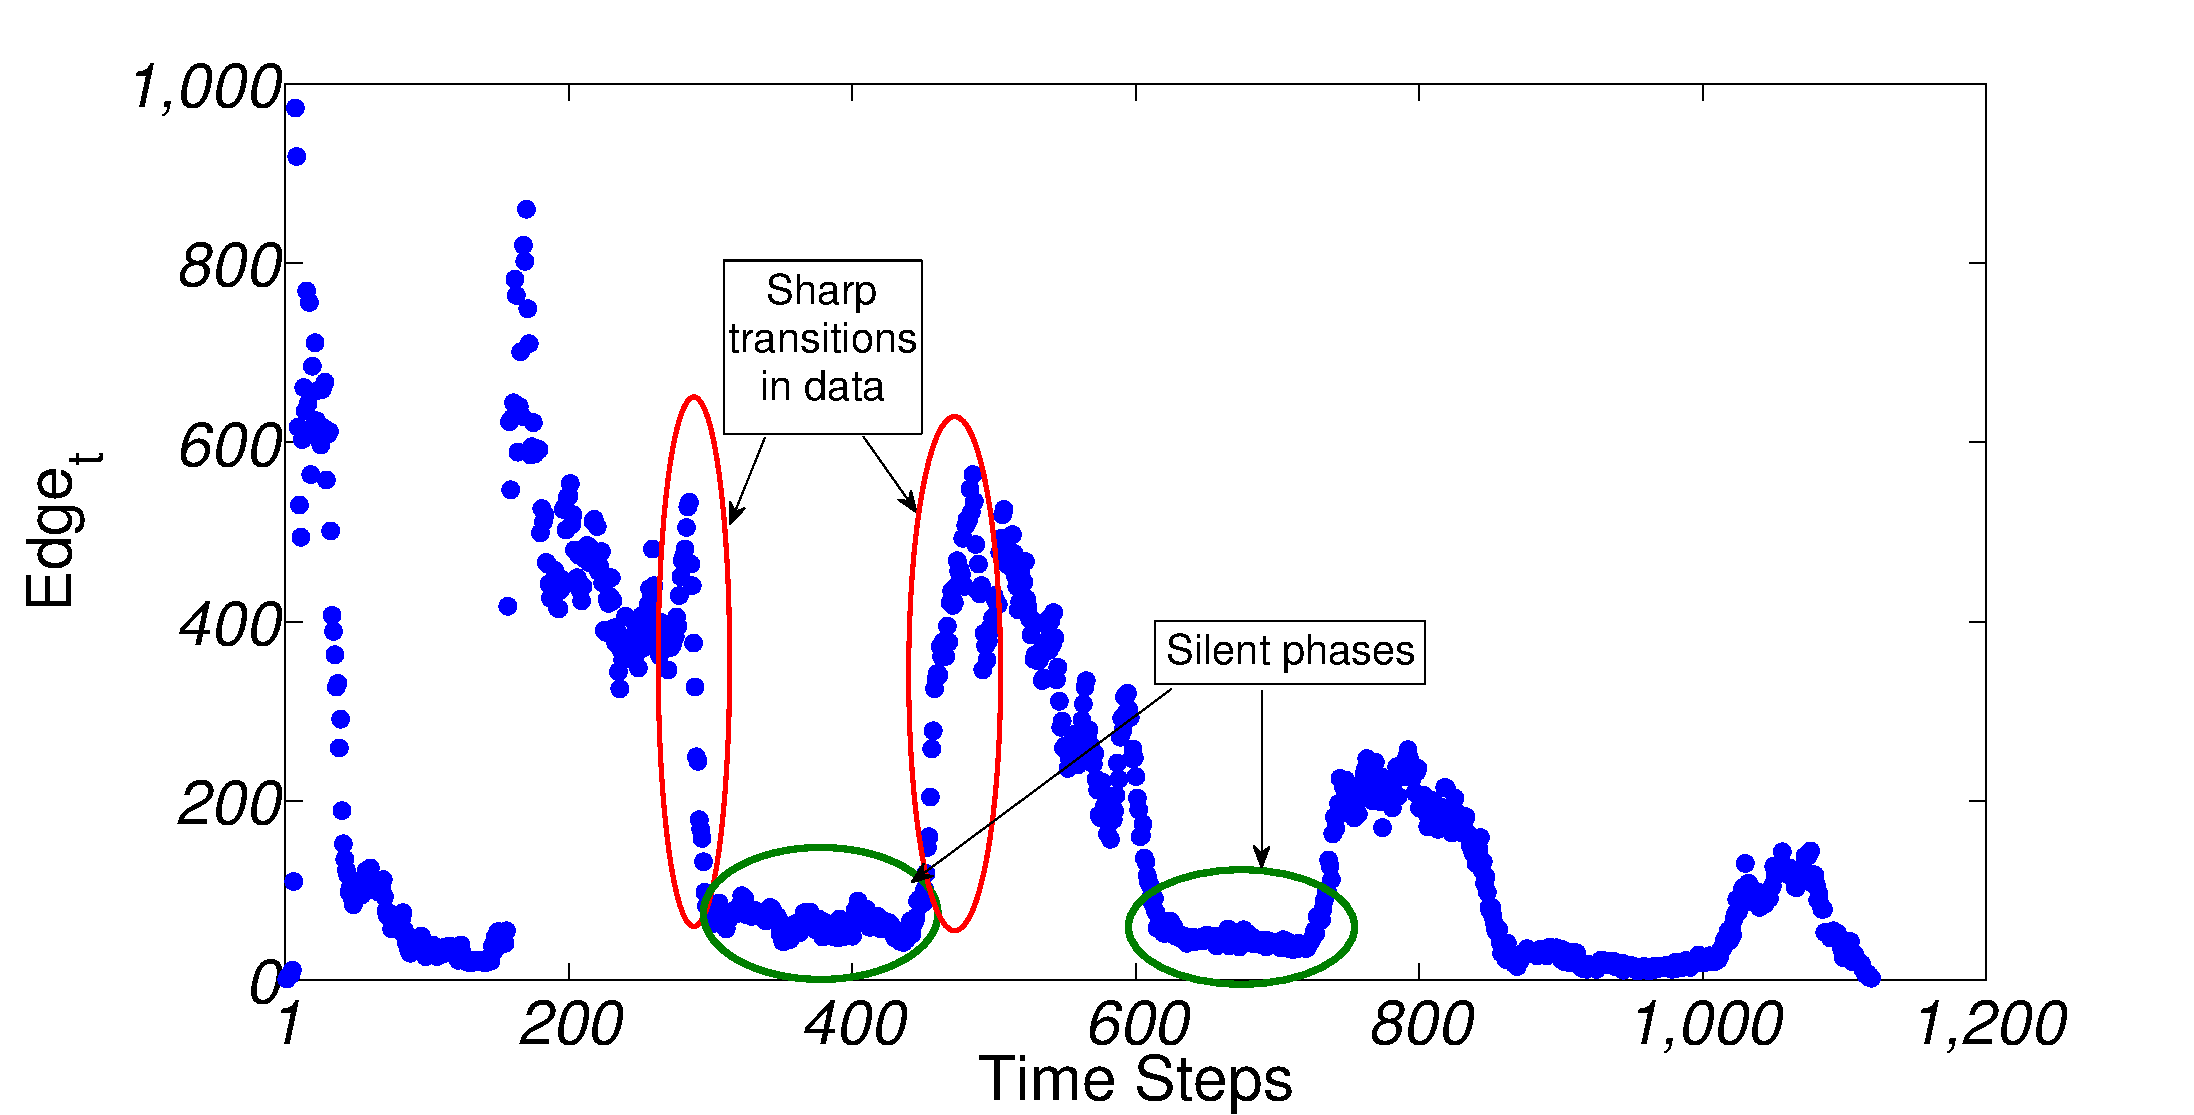
\includegraphics[width=0.7\columnwidth, angle=0]{./texfiles/Chapter_1/fig/no_of_edges1-eps-converted-to.pdf}
  \caption{\label{fig9}The time series plot for number of active edges. The red and the green ellipses identify
  two transition and two silent phases respectively}
  \end{center}
 \end{figure}

%  \begin{figure}
%  \begin{center}
%  \includegraphics[width=0.89\columnwidth, angle=0]{fig/psd_pred-eps-converted-to.pdf}
%  \caption{\label{k1}(A) LPSD versus mean percentage error for all the properties across all the datasets.}
%   \end{center}
%  \end{figure}
%\todo{Make Fig 10 more square -- otherwise difficult to understand}
 
 \begin{figure}[!ht]
  \begin{center}
  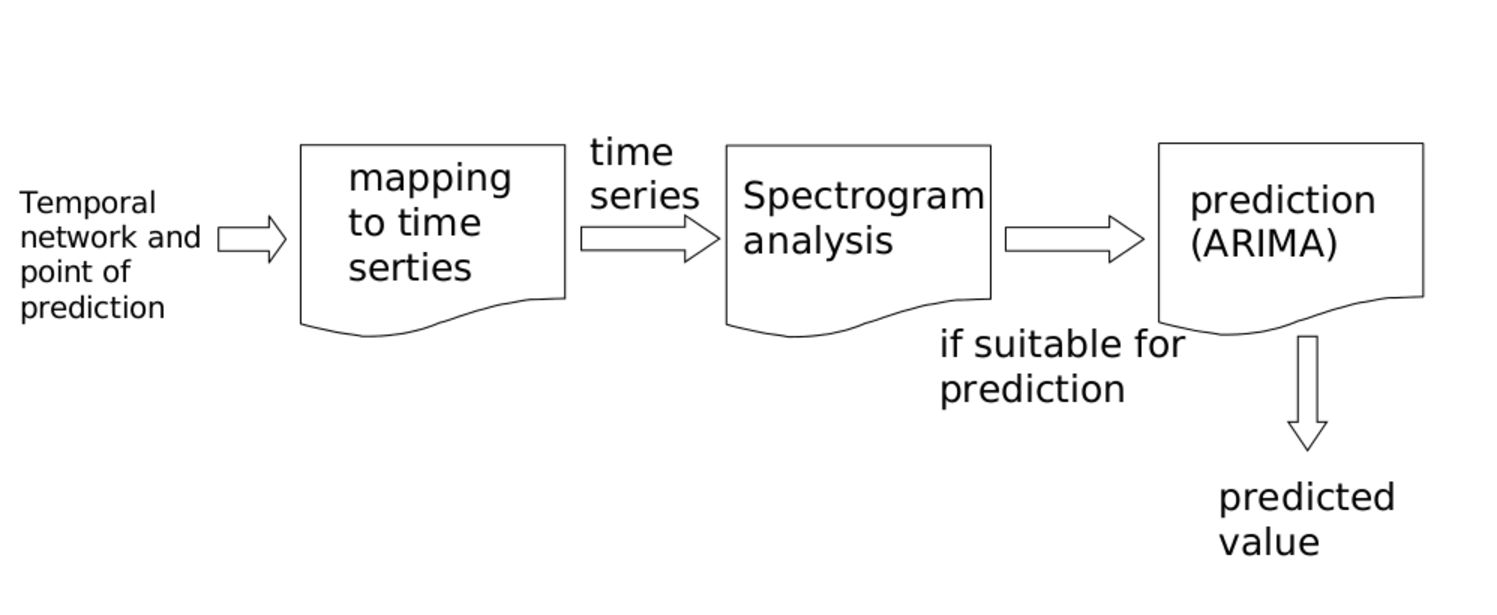
\includegraphics[width=0.95\columnwidth, angle=0]{./texfiles/Chapter_1/fig/Prediction.pdf}
  \caption{\label{fig:e_pred}The prediction framework.}
  \end{center}
 \end{figure}


%\subsection{Capturing the high error points}
%We next concentrate on the time points where the prediction error is high. 
% For the 600 time steps we considered, only in case of 8 time points for INFOCOM 2006 dataset and 32 time points in case of SIGCOMM 2009 dataset, did we find 
% more than five of the eight properties to give prediction error percentage more than 20\%. 
% \textcolor{blue}{Once again the error level chosen is representative and similar results are obtained for 10\% and 30\% error levels.} 
% For High school 2012, High school 2011 and Hospital datasets the corresponding 
% numbers are 42, 38 and 52 respectively.
% We observe that these points are mostly located either in places where a sharp transition occurred or in silent phases where there was limited interaction among the nodes.
% % On further 
% % investigation we find them to be either in places where a sharp transition has occurred or in the silent phases where there are have been limited interaction among the nodes.
% Figure~\ref{fig9} identifies some of the transition and silent phases in the time series of number of active edges in INFOCOM 2006 dataset.
% Similar phases are also present in the other datasets as well. 
% Next we check whether we can identify these points beforehand.
% These transition phases or silent phases are the idiosyncrasies of the dataset. 
% Since we are using human communication network, transition phases occur mostly due to the bursty nature of the network.
% We believe that our strategy will give even better result for datasets with higher stationarity. 
\begin{figure*}[!ht]
  \begin{center}
  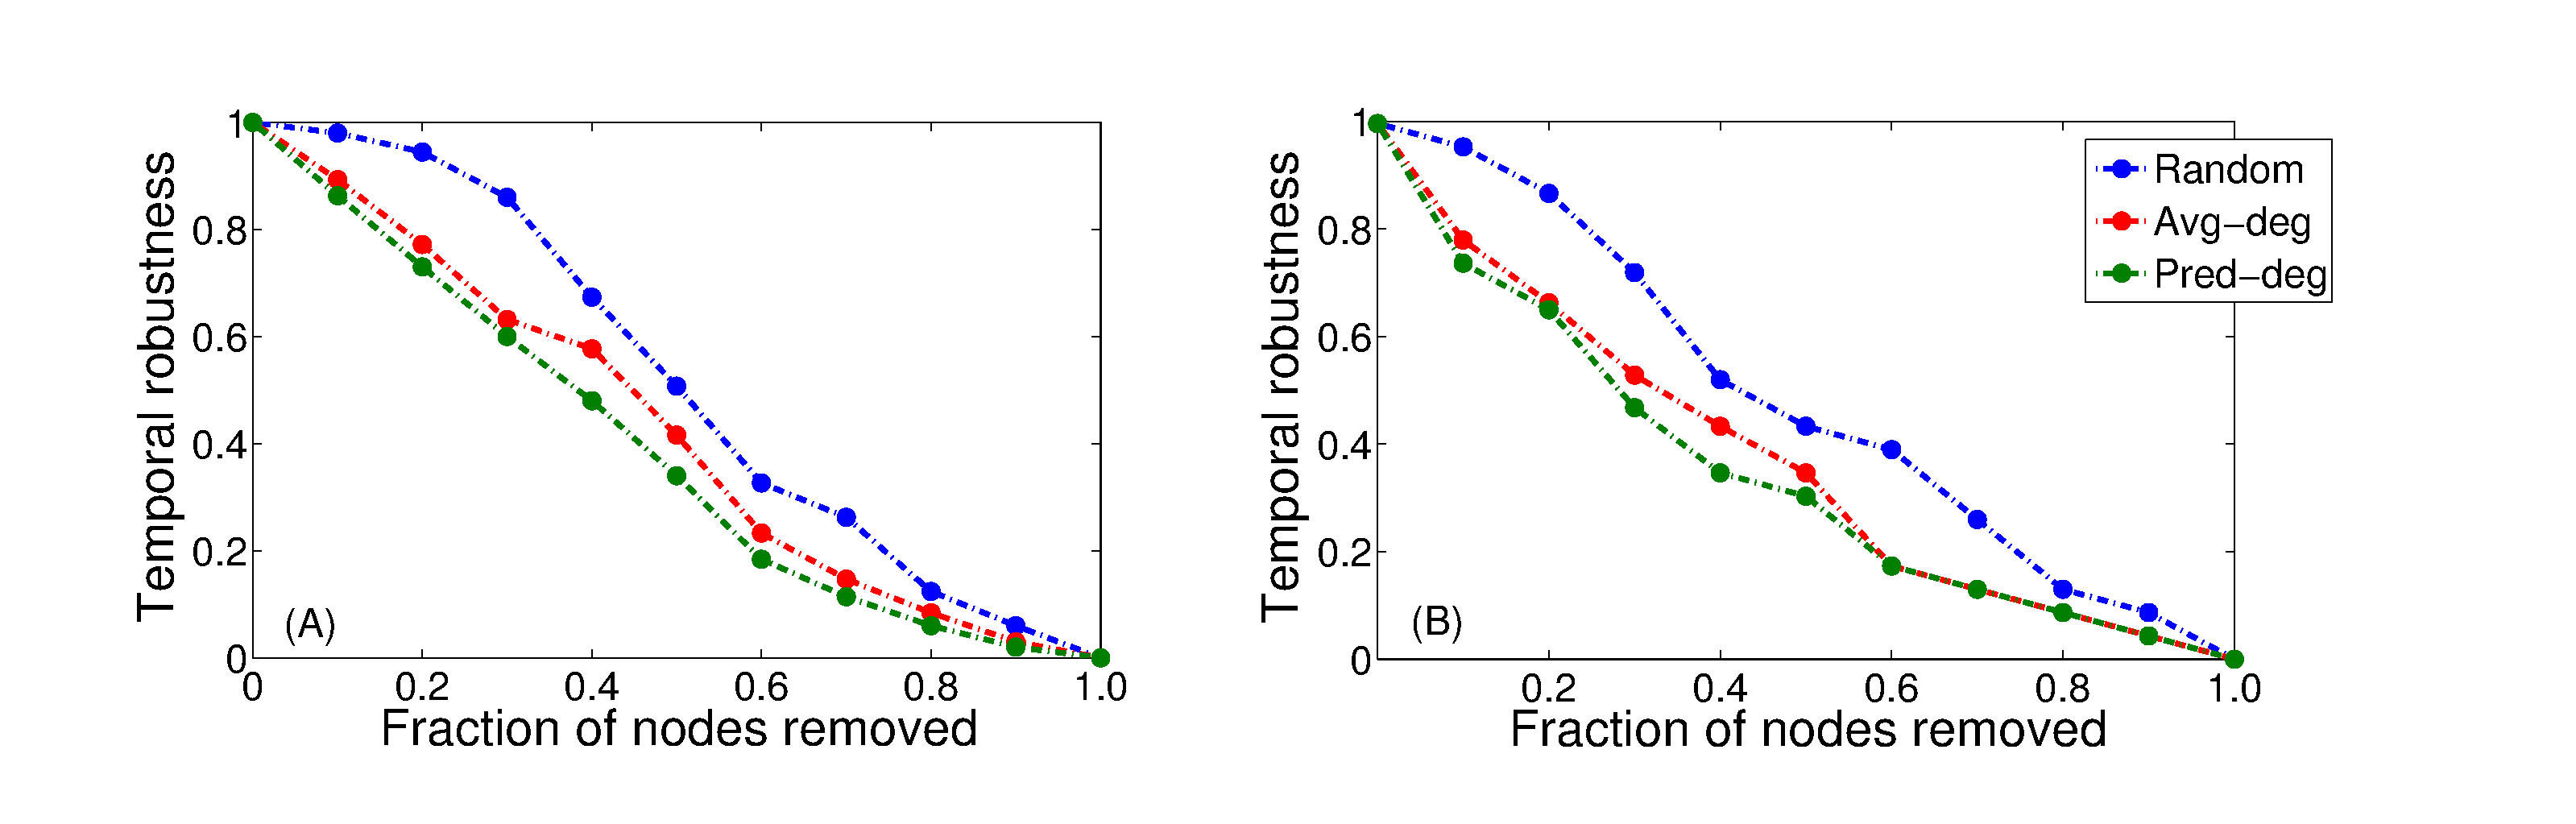
\includegraphics[width=0.9\linewidth, angle=0]{./texfiles/Chapter_1/fig/attack_all-eps-converted-to.pdf}
  \caption{\label{fig_attack}Temporal robustness as a function of the fraction of removed nodes for (a) INFOCOM 2006 and (b) SIGCOMM 2009 datasets.}
  \end{center}
 \end{figure*}

 
% Previously we have seen that spectrogram analysis on the time series of the properties is able to separate out the properties which are predictable (low errors in prediction). 
% We further plot the 
% mean percentage error against the mean PSD of frequencies $<$ 5 Hz (bin 1) in figure ~\ref{k1}(A). The plot clearly shows that the higher the value LPSD lower is the 
% mean percentage error and vice versa. Thus through the spectrogram of the time series we can conclude whether a property can be predicted 
% with low percentage error in prediction.
% To check whether the prediction at a time point would be erroneous, we extend the spectrogram analysis to the single point case. 
% While predicting a property at a give time step, we find that the spectrogram of the window ($w$) can be an 
% indicator for prediction accuracy. To our aim we consider two time steps: one where the prediction error is low and other where it is high for the property 
% number of active edges (INFOCOM 2006 dataset).
% In figure ~\ref{k1}(B) we plot the corresponding mean PSD value for the frequencies $<$ 5 Hz (bin 1) 
% for the two time steps. We observe 
% that the mean PSD value corresponding to the frequencies $<$ 5 Hz (bin 1) to be much higher in case where the prediction error is low (1) than 
% in the case where the prediction error was high (2). In fact this method could identify most of the points which where present in the transition or silent phase. 
% All these observations lead us to believe that spectrogram analysis can be used to filter out cases where the prediction error is high and thereby improve 
% the overall accuracy of our prediction framework.
 
 
 
\subsection{Enhancing the prediction scheme through spectrogram}

Since spectrogram analysis of the time series could determine the predictability of the corresponding property, 
an immediate extension would be to check whether it could be leveraged to identify beforehand the cases where the prediction error is high (unsuitable for prediction). 
To that aim we extend the spectrogram analysis to the single point case whereby  
 while predicting a property at a give time step, we find that the spectrogram of the window ($w$) and use the LPSD value as an indicator for potential prediction accuracy. 
 The cases identified by spectrogram analysis to be unsuitable for prediction can then be filtered out to improve the overall accuracy of the prediction framework. 
  A schematic diagram of this enhanced prediction framework is 
 provided in figure ~\ref{fig:e_pred}.
We now consider all the datasets and the corresponding time steps for prediction (which we considered earlier in this section, refer to table 3.1) and  
instead of directly using our prediction framework we 
 perform spectrogram analysis (single point method) on these points to separate out those which are unsuitable for prediction. We predict 
 only the points which the spectrogram analysis identifies as suitable for prediction.
 In table ~\ref{tab_res} we compare the fraction of predictions with 
 error $\leq 20\%$ between both the cases where we do not use spectrogram  and where we make use of it. 
 We observe that the fraction of prediction with error $\leq 20\%$ is enhanced for all the properties, albeit only marginally in some cases where the accuracy has already been high. 
 More importantly, for (ill-predicted) properties like betweenness centrality, closeness centrality, the prediction
accuracy increases substantially. 
 Note that prediction error $20\%$ is again representative and similar results 
 could be obtained for other values of prediction error as well.

% \subsubsection{Human interaction through social media}
% 
% \textcolor{blue}{We also applied our framework for the Twitter hashtag co-occurrence (London olympics) dataset for the properties for which short term correlation was present.
% We fixed the range of time steps between 100 and 600 and the average value of the fraction of predictions with percentage error less than or equal to 20\% 
% is 0.48. In table ~\ref{tab_twt} we report the detailed results. 
% As mentioned earlier we donot apply our prediction framework on the Facebook posts dataset.}
% 
% \begin{table}[h]
% \begin{tabular}{|c|c|c|c|c|c|c|}
% \hline
% \multirow{2}{*}{Network features} & \multicolumn{6}{l|}{Percentage error}                                     \\ \cline{2-7} 
%                                   & \multicolumn{3}{l|}{\textless=10\%} & \multicolumn{3}{l|}{\textless=20\%} \\ \hline
% Number of active nodes            & \multicolumn{3}{l|}{0.33}           & \multicolumn{3}{l|}{0.551}           \\ \hline
% Number of active edges            & \multicolumn{3}{l|}{0.294}          & \multicolumn{3}{l|}{0.494}           \\ \hline
% Average degree                    & \multicolumn{3}{l|}{0.276}          & \multicolumn{3}{l|}{0.517}          \\ \hline
% Clustering coefficient            & \multicolumn{3}{l|}{0.216}          & \multicolumn{3}{l|}{0.401}               \\ \hline
% Average            & \multicolumn{3}{l|}{0.275}          & \multicolumn{3}{l|}{0.485}               \\ \hline
% \end{tabular}
% \caption{\label{tab_twt}Network property and the fraction of predictions with percentage error less than or equal to 10\% and 20\% for Twitter hastag co-occurrence 
% network.}
% \end{table}

\medskip


\noindent
% \begin{figure*}[!ht]
%   \begin{center}
%   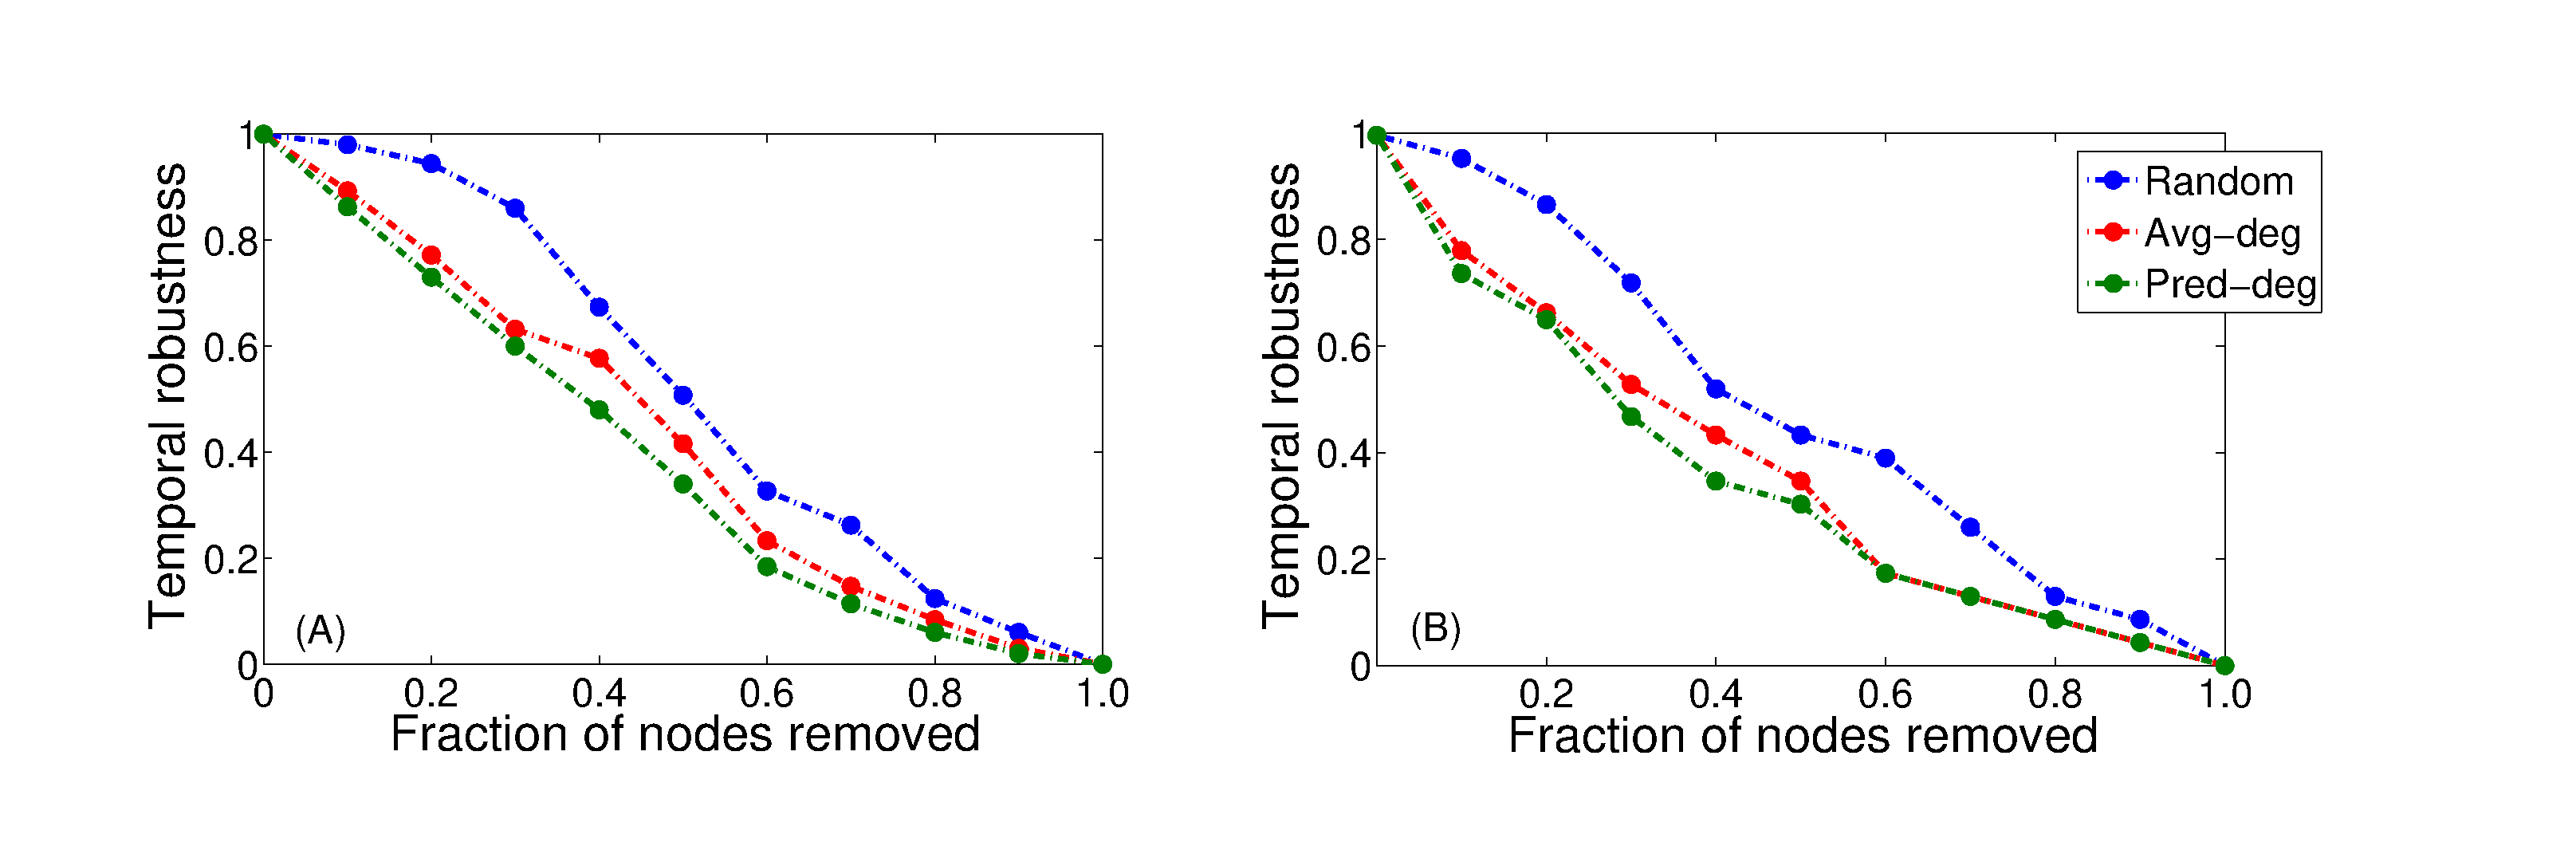
\includegraphics[width=0.9\linewidth, angle=0]{fig/attack_all.eps}
%   \caption{\label{fig_attack}Temporal robustness as a function of the fraction of removed nodes for (a) INFOCOM 2006 and (b) SIGCOMM 2009 datasets.}
%   \end{center}
%  \end{figure*}

\section{An attack strategy using prediction framework}
\label{attack}
%\todo{Be careful to have the window size `w' to be same for all the techniques -- I think thisis not there}
In this section we show how our prediction can be used in order to launch targeted attack on temporal networks. The strategy proposed is a modification over the average node degree attack presented in ~\cite{trajanovski2012error}. 
In case of average node degree attack the temporal degree\footnote{Given a time interval [$t_1, t_n$] temporal degree of node $i$ is the average degree of $i$ over the time interval}  
~\cite{trajanovski2012error} of the nodes are calculated and the node with highest temporal degree is removed in the 
subsequent steps (i.e., ``the node is attacked''). 
We observe that for every 
node its degree over a given time interval forms a time series. Using our prediction framework we calculate the degree of the node at a future time step based on the previous 
$w$ time steps (window size for the corresponding dataset, refer to section \ref{prediction})
and remove a node with the 
highest degree as predicted by our proposed framework. We compare our strategy (Pred-deg) with average node degree based attack (Avg-deg) and the random case (nodes are selected at random 
and removed). 
The effectiveness of an attack strategy is measured using temporal robustness ~\cite{trajanovski2012error} which is estimated by the relative change in efficiency ~\cite{trajanovski2012error} 
after a structural damage $D$. 
Temporal efficiency of a network $G$ in a given time interval [$t_1,t_n$], $E_G(t_1,t_2)$ is defined as the averaged sum of the inverse temporal distances over all pairs of 
nodes in that time interval. 
\begin{center}
 $E_G(t_1,t_2)=\frac{1}{N(N-1)}\Sigma_{i,j:i\neq j}\frac{1}{d_{ij}(t_1,t_2)}$
\end{center}
Here $N$ is the number of nodes in the network and $d_{ij}(t_1,t_2)$ is the temporal distance which is the smallest temporal length paths among all the temporal
paths between $i$ and $j$ in the time interval [$t_1,t_2$]. Hence, temporal robustness is defined  as $R_G(D)=\frac{E_{GD}}{E_G}$. 
In figure~\ref{fig_attack} we plot temporal robustness 
as a function of the fraction of nodes ($P$) removed 
for (a) INFOCOM 2006 and (b) SIGCOMM 2009 datasets. 
We observe that our strategy 
does better than both the random and average node degree based strategy. 

\if{0}
The reason for this result is straightforward. In the original average node degree based attack one averages 
the degree of a node for $n$ previous time steps and uses the value to rank the nodes of the $(n+1)^{st}$ time step (test data) and removes the top $P$ fraction of nodes. 
In our method, we use the actual degree values of the previous $n$ steps (training data), visualize them as a time series and predict the degree values of the $(n+1)^{st}$ step. The scheme based on 
the predicted degree values (which are pretty accurate estimates of the actual degree values of the $(n+1)^{st}$) is expected to produce a better ranking than the state-of-the-art 
scheme. As an additional advantage spectrogram analysis can also separate out the cases where our strategy would not work. 
Note that similar attack strategies could be developed based on other network properties as well.
We believe that our framework can be used as a better ranking scheme for nodes in a temporal network at a future time instant even if the network structure itself at that time point 
is unknown.
% \begin{figure*}[!ht]
%   \begin{center}
%   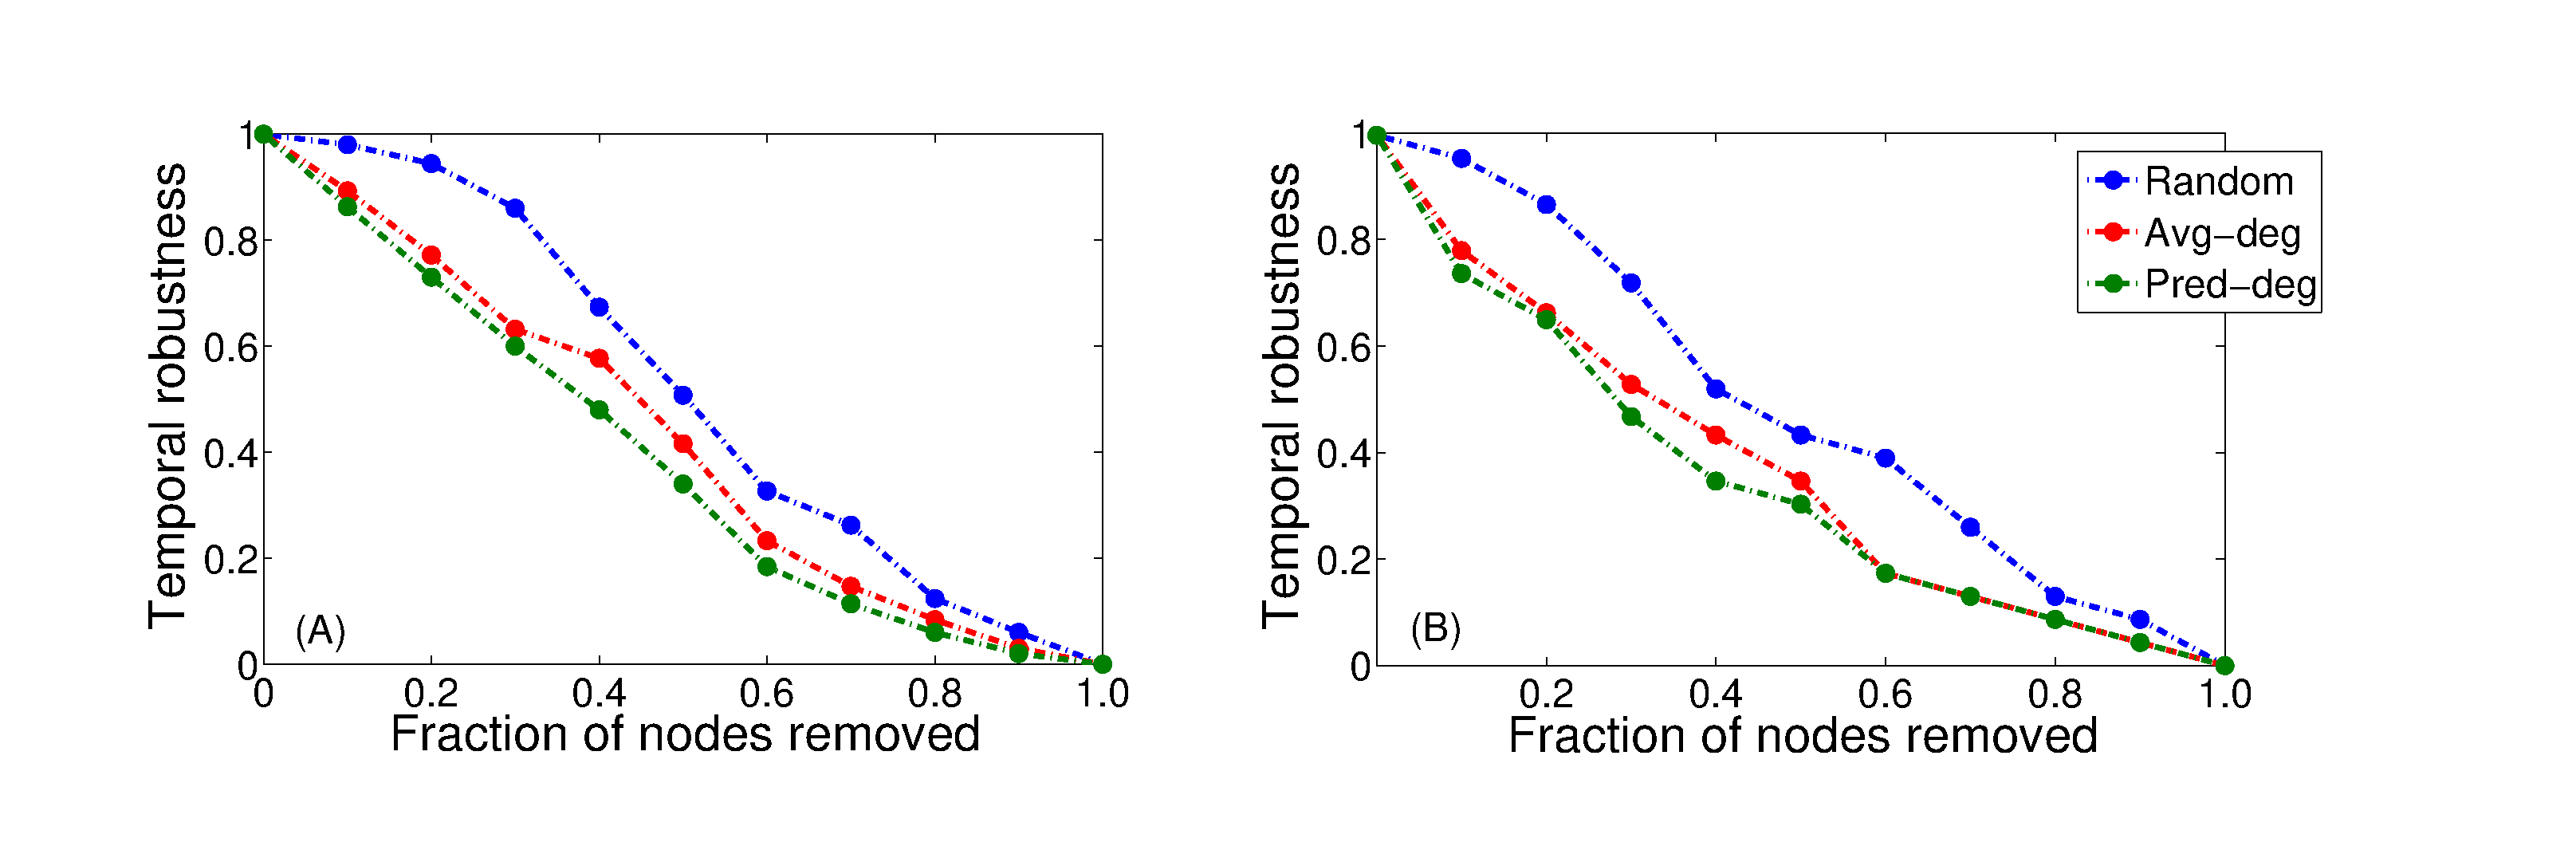
\includegraphics[width=0.9\columnwidth, angle=0]{fig/attack_all.eps}
%   \caption{\label{fig_attack}Temporal robustness as a function of the fraction of removed nodes for (a) INFOCOM 2006 and (b) SIGCOMM 2009 datasets.}
%   \end{center}
%  \end{figure*}
\fi


% \todo{This section is not needed -- remove}
% \subsection{Insights}  
% \label{insights}
% %\textcolor{blue}{
% \begin{itemize}
% %  \item Based on our analysis we can conclude that temporals networks representing human interactions can be sub divided into a two different classes. The datasets INFOCOM 2006 and 
% %  SIGCOMM 2009 which represent human face-to-face interaction differ significantly from the Twitter hashtag co-occurrence and the Facebook posts dataset 
% %  which represent human communication through social media. 
% %  Unlike the previous cases the 
% %  Twitter hashtag co-occurrence network is memory-less and almost no structural correlation exists. 
% %  For Facebook posts network also we find the network to be memory-less with only few of the properties showing presence of auto-correlation.
%  %From our analysis we are able to identify more than one class of temporal networks (we identify at least two here) and also conclude that not all temporal networks show structural 
%  %correlation.
%  \item 
% \todo{ Something like this may come just after prediction - I have diccussed with SS}
% We observe that the structural properties of a temporal network can be classified based on how well they can be predicted. We further observe that for 
%  both the datasets edge-emergence and number of active nodes give the best prediction result while betweenness centrality offers the worst prediction result.
%   This can be attributed to the fact that 
%  a person (node) who is a part of a conversation (network) at a time instant will remain a part of it in the next few time instances with high probability.
%  However, the node being a part of many shortest paths is a far rare event. 
% \todo{If you want you can mention it passingly in the conclusion}
%  \item In its current state our framework can predict the values of the network properties at a future time step but is unable to offer the exact network 
%  structure at that time step. But our framework can have genuine contributions toward link prediction in temporal networks. Since we show that structural 
%  correlation exists in these networks and we can also predict the network properties at these time steps as well, we can re-frame the link prediction problem 
%  as a network at a time step which is obtained from the network at a previous time step with minimal changes made depending on the values of the properties. 
%  We plan to deeply investigate this problem in subsequent works.
% \end{itemize}
% %}

% \subsection{An attack strategy using prediction framework}
% In this section we propose an attack strategy using based on our prediction framework. The strategy proposed is a modification over the average node degree attack. In case 
% of average node degree attack the temporal degree ~\cite{trajanovski2012error} of the nodes are calculated and node with highest temporal degree is attacked. We observe that given a 
% node its degree over a given time interval forms a time series. Using our prediction frame work we calculate the degree of the node at a future time step and remove a node with the 
% highest degree as obtained from the frame work. We compare out strategy (Pred-deg) with average node degree based attack (Avg-deg) and the random case (nodes are selected at random 
% and removed). In figure ~\ref{fig_attack} we plot temporal robustness ~\cite{trajanovski2012error} as a function of the fraction of nodes removed for Infocom 2006 dataset. We observe that our strategy 
% does better than both the random and average node degree based strategy. Note that similar attack strategies could be developed based on other network properties as well.
% 
% \begin{figure}[!ht]
%   \begin{center}
%   \includegraphics[width=0.7\columnwidth, angle=0]{fig/attack.eps}
%   \caption{\label{fig_attack}Temporal robustness as a function of the fraction of removed nodes for Infocom 2006 dataset.}
%   \end{center}
%  \end{figure}


\medskip


\noindent
\section{Summary of this chapter}
\label{conclusion}

Our contributions in this chapter can be summarized as below:
\begin{itemize}

\item we provided a general framework to map temporal network of human contacts consisting of a series of graphlets equispaced in time into time series
and provide a detailed time domain and frequency domain analysis.

\item we re-established the presence of structural correlation in a temporal network of human face-to-face contact using a new metric which we call
neighborhood-overlap.

\item we further quantified the extent of this correlation using neighborhood-overlap and used it to identify the correct window size in our prediction framework.

\item we also provided an approach for predicting the properties of future network instances using time series as a proxy and showed that even though the 
precise network structure is not known at time step, one can estimate its properties.

\item finally, we provided a frequency domain analysis of temporal network and leveraged it to enhance the prediction accuracy.

\item as an application we showed how our framework could be used in devising better strategies for targeted network attacks.
 
 \end{itemize}
 
 In its current state our framework can predict the values of the network properties at a future time step but is unable to offer the exact network 
 structure at that time step. But our framework can have genuine contributions toward link prediction in temporal networks. Since we show that structural 
 correlation exists in these networks and we can also predict the network properties at these time steps as well, we can re-frame the link prediction problem 
 as a network at a time step which is obtained from the network at a previous time step with minimal changes made depending on the values of the properties. 


\medskip

% \bibliographystyle{unsrt}


%\bibliography{ref}



%\end{document}

% end of file template.tex


%\cleardoublepage
\clearpage
\clearpage
% 
% \documentclass{sig-alternate-05-2015}
%  \usepackage[linesnumbered,ruled,vlined]{algorithm2e}
% % \usepackage{color}
% % \usepackage[table,xcdraw]{xcolor}
% % \usepackage{colortbl}
%  \newtheorem{prop}{Proposition}
%  \newtheorem{mydef}{Definition}
% % \usepackage{adjustbox}
%  \newcommand{\compas}{{\tt ComPAS}}
% % \newcommand\TODO[1]{\textcolor{red}{#1}}
% % \usepackage{multirow}
% % \usepackage{hyperref}
%  \usepackage[table,xcdraw]{xcolor}
% \usepackage{colortbl}
% \usepackage{times}
% \usepackage[linesnumbered,ruled,vlined]{algorithm2e}
% \usepackage{color}
% \usepackage[table,xcdraw]{xcolor}
% \usepackage{colortbl}
% \usepackage{amsmath,amsthm}
\newtheorem{prop}{Proposition}
\newtheorem{mydef}{Sampling problem}
% \usepackage{adjustbox}
% \newcommand{\compas}{{\tt ComPAS}}
% \newcommand\TODO[1]{\textcolor{red}{#1}}
% \newcommand\tbr[1]{\textcolor{brown}{#1}}
% \usepackage{multirow}
% \usepackage[draft]{hyperref}
% \usepackage[table,xcdraw]{xcolor}
% \usepackage{colortbl}
%\usepackage{amsmath,amsthm}


\newenvironment{function1}[1][htb]
  {\renewcommand{\thealgocf}{1}
  \renewcommand{\algorithmcfname}{Function}% Update algorithm name
   \begin{algorithm}
  }{\end{algorithm}}  
  
  
\newenvironment{function2}[1][htb]
  {\renewcommand{\thealgocf}{2}
  \renewcommand{\algorithmcfname}{Function}% Update algorithm name
   \begin{algorithm}
  }{\end{algorithm}}  
  
  \newenvironment{function3}[1][htb]
  {\renewcommand{\thealgocf}{3}
  \renewcommand{\algorithmcfname}{Function}% Update algorithm name
   \begin{algorithm}
  }{\end{algorithm}}  
  

\newenvironment{function4}[1][htb]
  {\renewcommand{\thealgocf}{4}
  \renewcommand{\algorithmcfname}{Function}% Update algorithm name
   \begin{algorithm}
  }{\end{algorithm}}  

\newenvironment{function5}[1][htb]
  {\renewcommand{\thealgocf}{5}
  \renewcommand{\algorithmcfname}{Function}% Update algorithm name
   \begin{algorithm}
  }{\end{algorithm}}
  
  \newenvironment{function6}[1][htb]
  {\renewcommand{\thealgocf}{6}
  \renewcommand{\algorithmcfname}{Function}% Update algorithm name
   \begin{algorithm}
  }{\end{algorithm}}
  
  \newenvironment{function7}[1][htb]
  {\renewcommand{\thealgocf}{7}
  \renewcommand{\algorithmcfname}{Function}% Update algorithm name
   \begin{algorithm}
  }{\end{algorithm}}
  \newenvironment{function8}[1][htb]
  {\renewcommand{\thealgocf}{8}
  \renewcommand{\algorithmcfname}{Function}% Update algorithm name
   \begin{algorithm}
  }{\end{algorithm}}

%\makeatletter
%\let\@copyrightspace\relax
%\makeatother


% \makeatletter
% \let\@copyrightspace\relax
% \makeatother
% 
% 
% \begin{document}
% 
% % Copyright
% \setcopyright{acmcopyright}
%\setcopyright{acmlicensed}
%\setcopyright{rightsretained}
%\setcopyright{usgov}
%\setcopyright{usgovmixed}
%\setcopyright{cagov}
%\setcopyright{cagovmixed}


\chapter{Sampling temporal graphs}

In the last chapter we developed a framework that could predict structural properties of a temporal network albeit we could not make any prediction regarding the 
structure of the network. It is in fact difficult to predict the structure of the network at a future time instant. We in this chapter look into a related problem - 
given a streaming graph, we obtain a sample of the graph which is most representative of its underlying structure. 
In specific, we obtain a sample that is able to preserve the underlying community structure. 


\vspace{-3mm}

\section{Introduction}

%\begin{enumerate}
%\item Although there are many existing graph sampling algorithms not all properties are represented correctly in the obtained sample. For example random not sampling is able to mimic the degree distribution of the original graph but fails to retain the clustering coefficient. We hence propose that separate sampling strategies should be designed in order to retain a specific property in the sample. We consider community structure i.e., we develop a sampling algorithm which retains the community structure of the original graph. The motivation behind such a algorithm is that generally community detection algorithm are generally computationally expensive and a sample which retains the community structure of the original graph would allow for running community detection algorithms on it and then extend it to the large graph thereby saving computing resources. It would be particularly helpful in cases where it is not known beforehand which community detection algorithm to use and hence all of them need to be executed in order to obtain the best result. One can run all the algorithms on the sample and decide on using a particular algorithm.

%\item As mentioned earlier community detection algorithms are computationally expensive and hence running them on large graphs could be very expensive. Our algorithm is designed in such a way that community detection algorithm is executed on a small scale and then community of a new node is decided incrementally. We thereby obtain a representative cluster structure which is computationally much less expensive. 
%\end{enumerate}
\if{0}
Sampling has been a fundamental part of statistics in is widely used in cases where it is difficult to perform analysis on the whole population. With proliferation of large scale graph data it is often required to measure properties of a large graph which are computationally very expensive. An obvious solution is to obtain a smaller representative sample of the graph and measure its properties assuming that the result would be similar to the original. But how to obtain a good representative sample? The question was first proposed in \cite{leskovec2006sampling} and the researchers have subsequently come up with several sampling algorithms \cite{ahmed2010reconsidering,maiya2010sampling,rasti2009respondent,ribeiro2010estimating}. Most of these works are mainly aimed at preserving specific graph properties. In \cite{maiya2010sampling} the authors argue that it is difficult to obtain a universally representative sample which preserves all the graph properties. 

Another interesting observation is that most of the real-world graphs evolve over time with new nodes and edges being added to the graph. Such graphs are represented through a streaming graph model whereby the 
\fi


Nowadays graphs are so large that their analysis in entirety can be intractable and impractical. How then one should proceed in analyzing and mining these graphs? Traditional approaches include designing more efficient algorithms or leveraging computing power through parallelization or distributed computing. Unfortunately, these existing methods are not always easily available as an option. Another approach that has received recent attention is the technique of {\em sampling}~\cite{leskovec2006sampling}.

Although data sampling is exhaustively studied in statistics~\cite{doucet2000sequential,hastings1970monte}, sampling from graphs has got only limited attention~\cite{gjoka2010walking,maiya2010sampling,rasti2009respondent,ribeiro2010estimating}. Moreover, when it comes to the case of sampling from {\em streaming graphs} (where edges arrive in discrete time intervals) there is hardly any work beside~\cite{aggarwal2011outlier,ahmed2014network}. 
Existing graph sampling methods are mostly designed for {\em static graphs} and aim at preserving general structural properties (such as degree distribution, clustering coefficient etc.) of the original graph in the sample. However we posit that it is impossible for any sampling method to produce a universal representation that can preserve {\em all} sorts of graph properties of the original graph; rather graph sampling should be {\em application specific}. For instance, sampling method designed for information diffusion should preserve the hubs (high-degree nodes) in the sample; whereas sampling for outbreak detection (such as disease outbreak) should preserve the nodes with high local clustering coefficient.

In this work, we propose a novel sampling algorithm that preserves the original {\em community structure}\footnote{In this work, we consider disjoint community structure.}. A community in a graph
is a cluster of nodes more densely connected among themselves than to others \cite{wasserman1994social}. Identifying community structure is important, as they represent the {\em mesoscopic view} of the graph and often correspond to real social groups, functional groups, or demographic similarity etc.~\cite{girvan2002community}. The ability to easily construct a sample consisting of members from diverse communities has several important applications. For instance, in marketing, surveys often seek to construct stratified
samples that collectively represent the diversity of the population \cite{Kolaczyk:2009}. Many popular community detection algorithms considered to be accurate are also computationally expensive~\cite{danon2005comparing,fortunato2010community}. Representative graph sampling, then, provides a potential solution for inferring and approximating global, latent properties such as these in large graphs. By sampling a representative subgraph, analysis can be performed on the sample instead of the larger graph. Results could, then, be generalized
to the larger population, which, in this case, is the original graph. However, if one still intends to run an accurate and computationally-expensive community detection algorithm on large graphs
and is confused which one algorithm to choose, she can run several potential algorithms on the sample graph and choose one that performs best. Then that algorithm can be used to detect communities from the original large graph.

{\bf Our contributions:} We propose~\compas, a novel sampling algorithm on streaming graph (most realistic graph representation \cite{aggarwal2011outlier,ahmed2014network}) that is capable of
representing and inferring community structure in the original graph. \compas~systematically interweaves graph sampling and community detection so that one gets benefits from the other to produce a more representative sample. In particular, our contributions are three-fold:
\begin{itemize}
\item To our knowledge \compas~is the first {\em community-preserving} sampling method for {\em streaming graphs}. Along with the sample, \compas~also produces the community structure of the sample.

\item Empirical evidences on synthetic graph and different real-world graph demonstrate that the sample generated by \compas~is not only the most representative to preserve the community structure, but also is quite competitive in reproducing the other general graph properties. %\TODO{Report numbers here. For instance, our results are x\% better in preserving the community structure compared to the most competitive baseline. Similarly report for other properties.}
The average performance of our algorithm reaches 85.5\% of the most informed algorithm (GA \cite{tong2016novel}) on static graphs.

\item We show additional benefits of \compas~through two applications -- (i) selection of right community detection algorithm for large graphs, and
%(ii) message spreading in streaming graph, 
(ii) selection of (limited) training set for online learning. We obtain a performance that is within 95.6\% and 90.5\% of the most informed algorithm (i.e., GA) available for static graphs for first and second applications respectively.
%\TODO{Are the benefits compared to some baselines? Then again report improvements here.}
\end{itemize}











%\noindent
\section{Related work}
\label{related_works}
The effectiveness of peer-review system has often been debated. Researchers have pointed out its several limitations~\cite{ingelfinger1974peer,relman1989good,smith2006peer}. 
In fact, authors in~\cite{cole1981chance} showed that 
reviewers often fail to reach consensus when judging the quality of the contribution while~\cite{braatz2014papers} points out that 
rejected papers are often cited more in the long run. Nevertheless, little work has been done toward systematic analysis and improvement of the 
system~\cite{graffy2006improving}. That blinding can improve the quality of the reviews, has been demonstrated in~\cite{mcnutt1990effects}.~\cite{caswellimproving} pointed 
out that incentives for reviewers could encourage them doing a better job. In~\cite{sikdar2016anomalies} the authors 
point out several indicators for anomalous behavior of the referees and the editors. In fact, they were able to filter out 
anomalous editors and reviewers leveraging anomaly detection algorithms. 

On the other hand, there have been a lot of work on the formation of teams of experts whose goal is to complete a given 
project~\cite{anagnostopoulos2010power,anagnostopoulos2012online, lappas2009finding,agrawal2014grouping,pragarauskas2012multi}. A trend in this line of work is to formulate
the team formation problem as an integer linear program
(ILP), and then focus on finding an optimal match
between people and the demanded functional requirements.
Widely used techniques in solving these problems include simulated
annealing~\cite{baykasoglu2007project}, branch-and-cut~\cite{zzkarian1999forming} or genetic algorithms~\cite{ani2010method}.~\cite{agrawal2014grouping} proposed 
a way of creating study groups in an educational setting so that the overall gain for the 
students is maximized. Another set of works leverage the underlying social network among the individuals as a proxy for compatibility and propose 
techniques for creating groups so as to match the requirements 
of a co-operative task~\cite{majumder2012capacitated,mcdonald2003recommending,wolf2009mining,li2010team}. 
In this paper we consider the review information of two leading scientific 
journals (JHEP -- Journal of High Energy Physics and JSTAT -- Journal of Statistical Mechanics: Theory and Experiment) and propose a scheme 
for allocating referees for a submitted paper. Anonymity of the reviewers and absence of any kind of underlying network 
prevents us from using any of the existing network based approaches. Formulating it as an ILP also appears difficult due to unavailability of any obvious optimization function.
To the best of our knowledge this is the first work which formulates the referee recommendation in peer-review system as a group formation problem 
leveraging genetic algorithms. We believe our findings could be useful in increasing the effectiveness of the peer-review system.

\begin{table}[]
\centering
\caption{Some general information related to the two datasets.}
\label{tab:data}
\scalebox{0.85}{
\begin{tabular}{l|l|l}
\hline
                                                                                      & JHEP  & JSTAT \\ \hline\hline
\# papers                                                                             & 28871 & 6106  \\ \hline
\# accepted papers                                                                    & 20384 & 3528  \\ \hline
\begin{tabular}[c]{@{}l@{}}Fraction of multi-reviewed \\ papers\end{tabular}           & 0.12  & 0.43  \\ \hline
\begin{tabular}[c]{@{}l@{}}\# Editors with at least one \\ assignment\end{tabular}    & 95    & 148   \\ \hline
\begin{tabular}[c]{@{}l@{}}\# Reviewers with at least \\ one assignment\end{tabular}  & 3976  & 2647     \\ \hline
\begin{tabular}[c]{@{}l@{}}Average number of \\ reviewers per paper\end{tabular}      &  1.03     & 1.42      \\ \hline
\begin{tabular}[c]{@{}l@{}}Average number of \\ authors per paper\end{tabular}        &  2.87     & 2.32      \\ \hline
\begin{tabular}[c]{@{}l@{}}Average number of \\ assignments per reviewer\end{tabular} &  6.48     &  2.56     \\ \hline
\# Unique keywords                                                                    & 201 & 562  \\ \hline
\end{tabular}}
\end{table}

\medskip


\section{Problem Definition}
\label{prob_def}

We consider a graph stream $S$ represented by a set of edges $e_1, e_2,...$ with each edge $e_i$ arriving at 
$i^{th}$ (discrete) time step. A graph $G$ at time $t$ is the aggregate of all the edges arriving till time $t$. 
$V$ represents the set of unique nodes present in  $G$. The community structure of $G$ is represented by $C$. We consider $G$ to be both unweighted and undirected. 
%We further assume that the edges are unique and they arrive in an order $O$. 

%\subsection{Sampling problem}

%\vspace{-3mm}
\begin{mydef}
Given a streaming graph $G$ and sample size $n$ in terms of the number of nodes, our objective is to obtain a sample graph $G_s$ such that $C$, the underlying community structure of $G$ is highly preserved in $G_s$  $($i.e., $C \sim C_s$ where $C_s$ is the community structure of $G_s)$. 
%\vspace{-5mm}
\end{mydef}



\setlength{\textfloatsep}{-3pt}% Remove \textfloatsep

\begin{algorithm}[htpb]

\caption{\compas: A {\bf Com}munity {\bf P}reserving Sampling {\bf A}lgorithm for {\bf S}treaming Graph}\label{alg:compas}
\KwData{$S$: Graph stream, $n$: Sample size,  $\alpha$: Initial fraction of nodes inserted, $n_d$: size of the buffer, $Algo$: a community detection algorithm}\label{algo_compas}
\KwResult{Sampled subgraph $G_s(V_s, E_s)$, $C_s$}
Initialize $G_s$: $V_s=\phi$, $E_s=\phi$\\
Create an empty buffer $\mathcal{H}$ of size $n_d$\\
Initialize buffer $\mathcal{H}$: $\mathcal{H}_c=\phi$, $\mathcal{H}_p=\phi$\\
$flag=1$, $t=0$\\
\For{$e_t$ in the graph stream $S$}{
$e_t=\{u,v\}$\\
%\If{$|V_s|\neq n$}{
\If{$\frac{|V_s|}{n}<\alpha \wedge e_t\notin E_s$}{\label{b:step1}
$V_s=V_s\cup u \cup v$\\
$E_s=E_s\cup e_t$\\
\textbf{Continue;}\label{e:step1}
}
\ElseIf{flag==1}{
Run $Algo$ on $G_s$ and detect community structure $C_s$\label{algo} \\
$flag$=0\\
}
\ElseIf{$u, v\in V_s$}{ 
$V_s,E_s,C_s=BothinSample(u,v,e_t,V_s,E_s,C_s)$\\
}
\ElseIf{$u,v\notin V_s \wedge u,v\in \mathcal{H}$}{
$\mathcal{H} = NodeinBuffer(u,\mathcal{H})$\\
$\mathcal{H} = NodeinBuffer(v,\mathcal{H})$
}
\ElseIf{$u \in V_s \wedge v\notin V_s \wedge v\in \mathcal{H}$}{
$\mathcal{H} = NodeinBuffer(v,\mathcal{H})$\\
%$V_s,E_s,C_s,\mathcal{H}=OneinSampleOneinBuffer(u,v,e_t,V_s,E_s,\mathcal{H},C_s)$
}
\ElseIf{$u\in V_s \wedge v\notin V_s \wedge v\notin \mathcal{H}$}{
$V_s,E_s,C_s,\mathcal{H}=NodeisNew(v,u,V_s,E_s,\mathcal{H},C_s)$
}
\ElseIf{$u\notin V_s \wedge u\in \mathcal{H} \wedge v\notin V_s \wedge v\notin \mathcal{H}$}{
$\mathcal{H}_c(u) = \mathcal{H}_c(u) +1$\\
$V_s,E_s,C_s,\mathcal{H}=NodeisNew(v,u,V_s,E_s,\mathcal{H},C_s)$
}
%\ElseIf{$u,v\notin V_s \wedge u,v\in \mathcal{H}$}{
%$\mathcal{H}_c[u]=\mathcal{H}_c[u]+1$\\
%$\mathcal{H}_c[v]=\mathcal{H}_c[u]+1$
%}
\ElseIf{$u,v\notin V_s \wedge u,v\notin \mathcal{H}$}{
$V_s,E_s,C_s,\mathcal{H}=NodeisNew(u,v,V_s,E_s,\mathcal{H},C_s)$\\
$V_s,E_s,C_s,\mathcal{H}=NodeisNew(v,u,V_s,E_s,\mathcal{H},C_s)$
}
$t=t+1$
}

%}
\Return $G_s$, $C_s$
\end{algorithm}



%\vspace{-2mm}

\section{Proposed algorithm: \compas}
\label{algorithm}

We propose \compas, a {\bf Com}munity {\bf P}reserving sampling {\bf A}lgorithm for {\bf S}treaming graphs. \compas~aims at sampling a streaming graph in such a way that its underlying community structure is preserved in the sample (Algorithm~\ref{algo_compas} and Figure~\ref{fig_algo} respectively present a pseudo-code and a toy example). 
The algorithm attempts to identify the high fidelity nodes (nodes with high degree and high clustering coefficient) and suitably determine the communities to which they belong. \\
%as these are the most suitable community centers and allow the sample to grow around them so that the important communities in the original graph are captured.} \\
{\bf Description of the algorithm:} To start with, \compas~keeps adding streaming edges (nodes) into the sample $G_s$ as long as a certain number  of nodes ($\alpha \cdot n$, $\alpha~<~1$) are inserted. 
This constitutes the warm-up knowledge for the structure. 
Once the threshold is reached, a pre-selected community detection algorithm $Algo$ is run on $G_s$ to obtain the {\bf initial community structure} (line \ref{algo}). 
%It then interweaves both graph sampling and community detection in such a way that each task gets benefits from the other. 

\noindent{\bf Subsequent dynamics:} Henceforth, once an edge $e_t$ is picked up from the stream, \compas~inserts $e_t$ into a buffer $\mathcal{H}$ (size $n_d$) which consists of the two variables -- $\mathcal{H}_c$ and $\mathcal{H}_p$. $\mathcal{H}_c$ counts 
%the ``number of hits'' of a node (i.e.,
the number of times a node is encountered till that time\footnote{In streaming graph, an edge might appear multiple times in the stream.}, and $\mathcal{H}_p$ keeps track of the current parent of a node (i.e., the node with which it arrived last). %\textcolor{blue}{
This presents a crude estimation of the importance of the node, since a recurrently occurring node is probably more important compared to a node occurring only intermittently. The idea is inspired by the reservoir sampling technique introduced in \cite{ahmed2014network}.
Once the buffer $\mathcal{H}$ is full, the insertion activity triggers some chain reactions which are different at the two specific phases 
(a). when the size of $G_s$ is between $\alpha \cdot n$ and $n$  -  any incoming new node triggers the entry of a node ($x$) and corresponding edge ($\mathcal {P}(x)$, $x$)  from buffer to $G_s$ and (b). when $G_s$ has already reached $n$ - at that point a node has to be removed from $G_s$ to insert the incoming node~($x$) from buffer. We eliminate the node with least degree and clustering coefficient thus  ensuring progressive
inclusion of high-fidelity nodes. 

\noindent{\bf Genesis of the six modules of \compas:} Considering differently, for an incoming  streaming edge $e_t~=~\{u,v\}$, each endpoint ($u,v$) could be (i) a new node, %(never encountered before or has got deleted), 
(ii) is present in the buffer or (iii) is present in the partially constructed  sample graph $G_s$. Depending on the current position of $u$ and $v$, one of the six conditions is encountered which are consequently handled by the six submodules - 
(1) both endpoints are present in the sample, (2) both are in buffer, (3) one is in sample while the other is in buffer, (4) one is in sample while the other is new, (5) one is in buffer while the other is new and (6) both are new. 
%A new node is always inserted into $\mathcal{H}$. As a result, (if $\mathcal{H}$ is full), we pick one node $x$ from $\mathcal{H}$ %preferentially based on $\mathcal{H}_c[x]$ with an additional constraint that $\mathcal{P}(x)$, the parent of $x$  should be in $G_s$\footnote{\tbr{this additional constraint allows to avoid a disconnected component being created in the sample and at the same time expanding one of the big components.}} (e.g., in Figure~\ref{fig_algo} if the buffer is full although node $l$ has highest count we do not pick $l$ from the buffer because its parent node $i$ is not in $G_s$; instead we pick $m$ which satisfies both the constraints). $x$ is then added to $G_s$ through the edge $\{\mathcal{P}(x),x\}$ and is and insert it into $G_s$, whereby, one node from $G_s$ is removed. The rules behind these insertions/deletions ensure that the fraction of the high fidelity nodes as well as the quality of the assigned communities improve progressively.  
%the community of $\mathcal{P}(x)$. If the node is already in the buffer, its frequency in incremented.  
%If $G_s$ is already full (i.e., $V_s=n$), one existing node which has lowest degree is removed from $G_s$ and the community structure 
%is adjusted accordingly using $CommunityAfterNodeRemoval()$ (both Functions 7 and 8 are discussed later).
We elaborate on the submodules next. 
%Note: we consider the situation where $|G_s|~=~n$ as well as $\mathcal{H}$ is full. 
%In order to maintain non-redundancy inside a community, \compas~never allows an existing  community to cross a certain edge density threshold $\beta$. 
%Throughout the iterations, \compas~maximizes {\em modularity}, a well-studied objective function for community detection defined as %\begin{equation}\label{modularity} {\small $Q(G(V,E),C)=\sum_{c\in C} (\frac{m_c}{M} - \frac{D_c^2}{4M^2})$} %\end{equation} where $C$ is the community structure of $G$, $m_c$ is the total number of edges inside $c$, $D_c$ is the sum of degree of all the nodes inside a community $c\in C$, and $M=|E|$ is the total number of edges $G$. In this section, we individually present each submodule of \compas~in details.\\ %Once the initial threshold $\alpha$ is reached, a community finding algorithm $Algo$ is used to detect the initial community structure of $G_s$ (denoted as $C_s$) (line 12). Then in every occurrence of a new edge $e_t=\{u,v\}$, it is not allowed to enter into the sample immediately; instead depending upon the current position of $u$ and $v$ different subroutines are invoked to place the edge (i.e., two end nodes) into the buffer {\color{red} redundant}.  %This in turn may remove an existing node out of the buffer and connect it with its parent in $G_s$. $C_s$ is adjusted accordingly. 
%/In this section, we describe different subroutines in details.

\noindent\textbf{(i) \underline{Both $u$ and $v$ are present in the Graph $G_s$:}} When both $u,v$ are in $V_s$, $BothinSample()$ (see Function \ref{bothsample}) is called from 
line 15 of Algorithm \ref{algo_compas}.  
The aim of this module is to place the edge in such a way that the modularity 
of the evolving sample graph ($G_s$) improves. Vis-a-vis the existing community structure, the edge $e_t$ 
%can either be an intra community edge or an inter community edge. Accordingly,    } 
%Note that all the above actions are aimed at selectively densifying the component and letting the community structure to evolve with maximizing modularity at the same time.}
%we have two subcases: $e_t$ is 
can be (a). an intra-community edge (totally inside a single community) or 
(b). an inter-community edge (connecting two communities $C(u)$ and $C(v)$). 

In case of an intra-community edge (edge $\{b,d\}$ in figure~\ref{fig_algo}), addition of $e_t$ 
increases modularity of the community according to Proposition~\ref{1}. Moreover, we also know from Proposition~\ref{2} that 
splitting of current community on addition of a new intra-community edge does not increase modularity~\cite{PhysRevE.78.046115}. 
Therefore we leave $C_s$ in its current form without any modification.

\begin{prop}\label{1}
%For a community $c\in C$, if $D_c\leq M-1$ $($where $M=|E|)$ then addition of an edge within $c$ will increase its modularity.
Addition of an edge to a community $c\in C$, increases its modularity if $D_c\leq M-1$ $($where $M=|E|$ and $D_c$ is total degree of all the nodes $c$ ).
%\vspace{-2mm}
\end{prop}


\begin{proof}
From definition of modularity, we see the contribution of individual community $c\in C$ in modularity as: $Q_c=\frac{m_c}{M} - \frac{D_c^2}{4M^2}$. 
%where $m_c$ is the number of edges inside $c$, $M$ is the total number of edges in the graph, and $D_c$ is the sum of degrees of all the nodes in $c$. 

Addition of a new edge within $c$, the $c$'s contribution of modularity becomes:
\[
Q'_c=\frac{m_c+1}{M+1} - \frac{(D_c+2)^2}{4(M+1)^2}
\]

So the increase in modularity is $\Delta Q_c=Q'_c-Q_c$,
\[
\begin{split}
\Delta Q_c=&\frac{4M^2-4m_cM^2-4D_cM^2-4m_cM+2D_c^2M+D_c^2}{4(M+1)^2M^2}\\
%&\geq \frac{4M^2-6D_cM^2-2D_cM+2D_c^2M+D_c^2}{4(M+1)^2M^2}\\
&\geq\frac{(2M^2-2D_cM-D_c)(2M-D_c)}{4(M+1)^2M^2}\\
&\geq 0
\end{split}
\]
The equality holds if $D_c\leq M-1$. This thus implies $(2M^2-2D_cM-D_c)\geq 0$. This proves the proposition.
\end{proof}

\begin{function1}[!ht]
%\caption{Both in Sample}
\caption{\small$BothinSample(u,v,e_t,V_s,E_s,C_s)$} \iffalse\TODO{Notation mismatch. Are $\Delta_{u,C_s(u),C_s(v)}$ and $\Delta Q(u, C_s(u),C_s(v))$ the same?} \textcolor{blue}{corrected}\fi
\label{bothsample} 
\If{$C_s(u)==C_s(v)$}{
$E_s=E_s\cup e_t$
}
\Else{
\If{$\Delta Q (u,C_s(u),C_s(v))<0 \wedge \Delta Q (v,C_s(v),C_s(u))<0 \wedge Q(\{u,v\},\{C(u),C(v)\},C^{\ast})<0$}{
\Return{$V_s,E_s,C_s$}}
\Else{
$w = arg max \{\Delta  Q(u,C_s(u),C_s(v)),\Delta Q(v,C_s(v),C_s(u))$, \\
$Q(\{u,v\},\{C(u),C(v)\},C^{\ast})\}$\\
Move $w$ to a new community and update $C_S$\\
\For{$t\in N(w)$}{
Let $t$ decide its own community 
%\textcolor{red}{Modify to address the question of referee 1.} \\
Update $C_s$
}
}
}
\Return $V_s,E_s,C_s$   
\end{function1}

\begin{prop}\label{2}
%For a community $c\in C$, addition of any intra-community edge into $c$ should not split it into smaller communities.
Addition of any intra-community edge into a community $c\in C$ would not split into smaller communities.
%\vspace{-2mm}
\end{prop}




\begin{proof}
We will prove this proposition by contradiction.
Assume that once a new intra-community edge is added into $c$, it gets split into $k$ small modules, namely $X_1$, $X_2$, $\cdot$,$X_k$. Let $D_{X_i}$ and $e_{ij}$ be the total degree of nodes inside $X_i$ and number of edges connecting $X_i$ and $X_j$ respectively. 


%Recall that the contribution of $X_i$ in the modularity value is $Q_{X_i}=\frac{m_{X_i}}{M} - \frac{D_{X_i}^2}{4M^2}$.  
Before adding the edge, we have $Q_c \geq \sum_{i=1}^k Q_{X_i}$ (where $Q_c$ is the total modularity of community $c$), because otherwise all $X_i$s can be split earlier, which is not in this case. This implies that: $\frac{m_c}{M}- \frac{D_c^2}{4M^2} > \sum_{i=1}^k (\frac{m_{X_i}}{M} - \frac{D_{X_i}^2}{4M^2})$. Since $X_1,X_2,\cdot,X_k$ are all disjoint modules of $c$, $D_c=\sum_{i=1}^k D_{X_i}$ and $m_c=\sum_{i=1}^k m_{X_i} + \sum_{i<j} e_{ij}$. This further implies that:
%\[ \frac{m_c}{M}-\sum_{i=1}^k \frac{m_{X_i}}{M} > \frac{D_c^2}{4M^2}- \sum_{i=1}^k \frac{D_{X_i}^2}{4M^2}\]
%or,
$\sum_{i<j} e_{ij} > \frac{\sum_{i<j} D_{X_i}D_{X_j}}{2M}
$.
 
 Without loss of generality, let us assume that the new edge is added inside $X_1$. 
Since we assume that after adding the new edge into $c$, it gets split into $k$ small modules, the modularity value should increase because of the split. Therefore, %Therefore, the new modularity $Q'_c<\sum_{i=1}^k Q_{X_i}$. 
%This implies that
\[
\begin{split}\small
& Q'_c < \sum_{i=1}^k Q_{X_i}\\
& \Leftrightarrow \frac{\sum_{i=1}^k m_{X_i} + \sum_{i<j} e_{ij} + 1}{M+1} - \frac{(\sum_{i=1}^k D_{X_i +2})^2}{4(M+1)^2}\\
%& <  \frac{m_{X_1}+1}{M+1} - \frac{(D_{X_1}+2)^2}{4(M+1)^2}  + \sum_{i=2}^k  (\frac{m_{X_i}}{M+1} - \frac{D_{X_i}^2}{4(M+1)^2} )\\
%&\Leftrightarrow \frac{\sum_{i=1}^k m_{X_i} + \sum_{i<j} e_{ij} + 1}{M+1} - \frac{(\sum_{i=1}^k D_{X_i +2})^2}{4(M+1)^2}\\
& < \frac{\sum_{i=1}^k m_{X_i}+1}{M+1} - \frac{(D_{X_1}+2)^2}{4(M+1)^2} - \sum_{i=2}^k \frac{D_{X_i}^2}{4(M+1)^2}\\
&\Leftrightarrow \sum_{i<i} e_{ij} < \frac{\sum_{i=1}^k D_{X_i} - 2 D_{X_1} + \sum_{i<j} D_{X_i}D_{X_j}}{2(M+1)}
\end{split}
\]
Since $\sum_{i=1}^k D_{X_i} - 2D_{X_1} < 2M$, this implies that 
\[\small
\begin{split}
\frac{\sum_{i<j}D_{X_i}D_{X_j}}{2M}  < \sum_{i<j}e_{ij} 
&< \frac{\sum_{i=1}^k D_{X_i} - 2D_{X_1} + \sum_{i\neq j}{D_{X_i}D_{X_j}}}{2(M+1)}\\
& <\frac{\sum_{i<j}D_{X_i}D_{X_j}}{2M}+1
\end{split}
\]
Thus, the proposition holds.
\end{proof}



In case of $e_t$ connecting two different communities (edge $\{b,f\}$ in Figure \ref{fig_algo}), three possibilities may arise - \\
(i) $u$ may leave its current community and join $v$'s community, (ii) $v$ may leave its current community and join $u$'s community and (iii) $u$ and $v$ may leave their current communities and together form a new community. In addition, if the community membership of $u$ (or $v$) is changed, this can also pull out its neighbors to join with it, and some of the neighbors might eventually want to change their memberships as well~\cite{pone.0091431}. To decide we first calculate $\Delta Q(u,C(u),C(v))$ (where $\Delta Q(x,C(x),C(y))$ indicates the change in modularity after assigning $x$ from $C(x)$ to $C(y)$) (case (i)), $\Delta Q(v,C(v),C(u))$ (case (ii)) and $\Delta Q(\{u,v\},\{C(u),C(v)\},C^{\ast})$ ($u$ and $v$ change their current communities to form a new community $C^{\ast}$, case (iii)) and select the case where the change in modularity is maximum. Consequently, we let the neighbors (of the node whose community membership is altered by the above action) decide their best move in the similar way. This continues recursively (neighbors of neighbors) until the modularity stabilizes or decreases.  
%(i) $u$ (or $v$) may leave its current community and join another community. 
%Additionally, if the community membership of $u$ (or $v$) is changed, it can also pull out its neighbors to join with it, and some of the neighbors might eventually want to change their memberships as well \cite{pone.0091431}. According to Proposition~\ref{3}, we know that if $u$ (or $v$) ever changes its community membership, $C(v)$ (or $C(u)$) would be the best new community for it. But how to decide it quickly? We calculate $\Delta Q(u,C(u),C(v))$  
%But how do we quickly decide it? Here we provide a criteria to check the change in membership for $u$ and $v$ in Proposition~\ref{complex}. If both $\Delta Q(u,C(u),C(v))$ and $\Delta Q(v,C(v),C(u))$ (where $\Delta Q(u,C(u),C(v))$ indicates the change in modularity after assigning $u$ from $C(u)$ to $C(v)$) fail to satisfy the criteria (see Corollary 1), we can retain the current community structure. Otherwise, we move $u$ (or $v$) to $C(v)$ (or $C(u)$) and consequently we let its neighbors decide their best move in the similar way. This continues recursively (neighbors of neighbors) until the modularity does not change or decreases. 
%\textcolor{red}{Tell that you are doing this recursively to address the question of referee 1.} %\textcolor{blue}{
%}


\begin{figure}[!t]
\centering
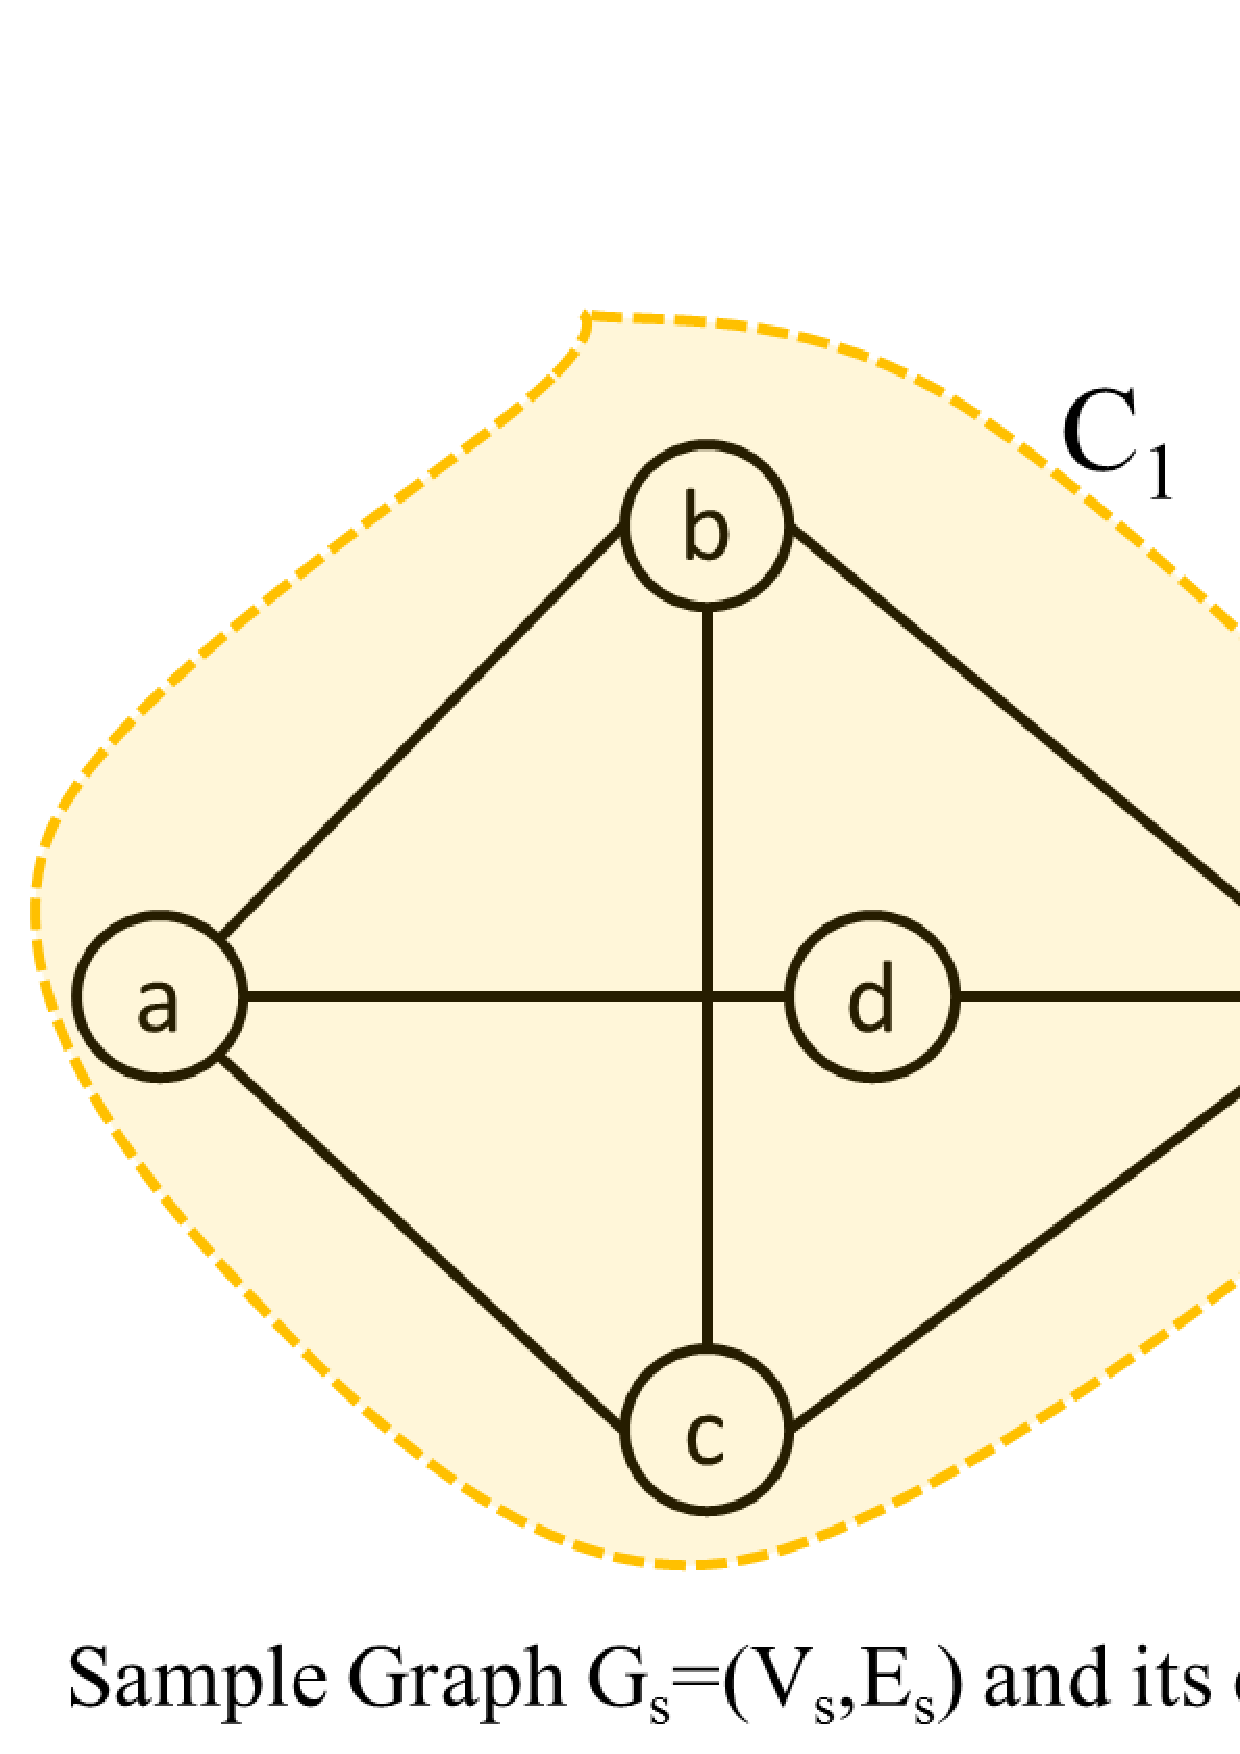
\includegraphics[width=0.8\columnwidth]{./texfiles/Chapter_2/figures/demo.pdf}
%\vspace{-5mm}
\caption{Toy example depicting various conditions handled by \compas~ when a streaming edge arrives.}\label{fig_algo} 
\vspace{2mm}
\end{figure}

%\vspace{-3mm}






\iffalse
\begin{prop}\label{3}
If a new inter-community edge $(u,v)$ connecting two communities $C(u)$ and $C(v)$ is introduced, $C(u)$ $($or $C(v))$ is the most likely candidate for $v$ (or $u$) if it changes its membership.
%\vspace{-2mm}
\end{prop}

\begin{proof}
The method is inspired by \cite{PhysRevE.78.046115} that a vertex $u$ is influenced by two factors: $F^c_{in}(u)$ the force that keeps $u$ stay in its own community $c$, and $F^c_{out}(u)$, the force that a community $S$ imposes to $u$ in order to bring $u$ to $S$ as follows:
\[\small
F^c_{in}(u)=e_c^u-\frac{d_u(D_c-d_u)}{2M}
\]
and 
\[\small
F^S_{out}(u)=max_{S\in NC(u)} \{e_S^u - \frac{d_u D_{outS}}{2M}\}
\]
where $NC(u)$ is the set of neighboring communities of $u$, and $D_{outS}$ is the total degree of vertices outside $S$.

Now we will show that the presence of new edge $(u,v)$ will strengthen $F^{C(v)}_{out}(u)$ and weaken $F^S_{out}(u)$. In other words, we will show that $F^{C(v)}_{out}(u)$ increases while $F^S_{out}(u)$ decreases for all $S \in C \wedge S \notin \{C(u),C(v)\}$.
\[\small
\begin{split}
&F^{C(v)}_{out}(u)|_{new} - F^{C(v)}_{out}(u)|_{old}\\
&=(e_u^{C(v)}+1-\frac{(d_u+1)(d_{outC(v)}+1)}{2(M+1)} - (e_u^{C(v)} - \frac{d_ud_{outC(v)}}{2M})\\
%&= \frac{2M+d_ud_{outC(v)}}{2(M+1)} - \frac{d_ud_{outC(v)}+d_{outD(v)}+d_u+1}{2(M+1)}\\
&\geq \frac{2M+d_ud_{outC(v)}}{2(M+1)} - \frac{d_u d_{outC(v)}+d_{outC(v)}+d_u+1}{2(M+1)}\\
&>0
\end{split}
\]
Therefore $F^{C(v)}_{out}(u)$ is strengthened when a new edge $(u,v)$ is introduced. Further, for any community $S\in C \wedge S\notin \{C(u),C(v)\}$
\[
\begin{split}
& F^{S}_{out}(u)|_{new} - F^{S}_{out}(u)|_{old}\\
&= (e^S_u-\frac{(d_u+1)d_{outS}}{2(M+1)}) - (e^S_u - \frac{d_ud_{outS}}{2M})\\
&= d_{outS}(\frac{d_u}{2M} - \frac{d_u+1}{2(M+1)})<0
\end{split}
\]

This implies that $F^S_{out}(u)$ is weakened when $(u,v)$ is added. Therefore,  the proposition holds.
\end{proof}
\fi


\iffalse
\begin{prop}\label{complex}
If a new edge $(u,v)$ is added into the graph, then joining $u$ to $v$'s  community $C(v)$ will increase the modularity value  if $\Delta Q(u,C(u),C(v)) \equiv 4(M+1)(e_{C(v)}^u+1-e_{C(u)}^u)+e_{C(v)}^u(2D_{C(v)}-2d_u-e_{C(u)}^u) - 2(d_u+1)(d_u+1+d_{C(v)}-d_{C(u)})>0$.
%\vspace{-2mm}
\end{prop}
\fi
\iffalse
\begin{proof}
Vertex $u$ will leave its current community $C(u)$ and join $v$'s community $C(v)$ if
\[\small
\begin{split}
& Q_{C(v)+u} + Q_{C(u)-u} > Q_{c(u)} + Q_{C(v)}\\
&\Leftrightarrow \frac{m_{C(v)}+e_{C(v)}+1}{M+1} - \frac{(d_{C(v)}+d_u+2)^2}{4(M+1)^2}+\\
&\frac{m_{C(u)} - e_{C(u)}}{M+1} - \frac{(d_{C(u)}-d_u-e_{C(u)})}{4(M+1)^2} \\
& > \frac{m_{C(v)}}{M+1} - \frac{(d_{C(v)}+d_u+2)^2}{4(M+1)^2} + \frac{m_{C(u)}}{M+1} - \frac{(d_{C(u)}+1)^2}{4(M+1)^2}\\
&\Leftrightarrow 4(M+1)(e_{C(v)} +1 -e_{C(u)}) + e_{C(u)}(2d_{C(v)} - 2d_{C(u)}-e_{C(u)})\\
& - 2(d_{C(u)}+1)(d_{C(u)}+1+d_{C(v)}-d_{C(u)})>0
\end{split}\]
\end{proof}
\fi
\iffalse
\noindent{\bf Corollary 1.} {\em If the condition in Proposition \ref{complex} is not satisfied, then neither $u$ nor its neighbors should be assigned to $C(v)$.}
\fi

%\vspace{-3mm}

%\vspace{-2mm}
\iffalse
\begin{function2}[!t]\tiny
\caption{\small$OneinSampleOneNew(u,v,e_t,V_s,E_s,\mathcal{H},C_s)$}
\label{onesampleonenew}
\If{$\mathcal{H}$ is not full}{
Insert $v$ to $\mathcal{H}$\\
}
\Else{
Choose a node $x$ with $\mathcal{P}(x) \in V_s$ from $\mathcal{H}$ preferentially based on $\mathcal{H}_c$\\
$V_s,E_s,C_s,\mathcal{H} = OneinSampleOneinBuffer(\mathcal{P}(x),x,V_s,E_s,\mathcal{H},C_s)$\\
%Remove $x$ from $\mathcal{H}$\\
%$\mathcal{H}_c[x]=0$\\
%$\mathcal{H}_p[x]=\phi$\\
%$V_s,E_s,C_s = CheckResizeSample(V_s,C_s,n,1)$\\
%$V_s=V_s\cup x$\\
%$E_s=E_s\cup \{P(x),x\}$\\
%$C_s(x)=C_s(P(x))$\\
%Update $C_s$\\ %\TODO{Not clear what this line does. I do not see a separate update function.}\\
%Insert $v$ to $\mathcal{H}$\\
}

$\mathcal{H}_c[v]=1$\\ 
$\mathcal{H}_p[v]=u$\\ 
\Return $V_s,E_s,C_s,\mathcal{H}$   
\end{function2}
\fi

\begin{function2}[!ht]
\caption{\small $NodeinBuffer(u,\mathcal{H})$}
\label{nodebuffer}
$\mathcal{H}_c[x]=\mathcal{H}_c[x] + 1$\\
\Return $\mathcal{H}$
\end{function2}



%\vspace{-3mm}


\noindent\textbf{(ii) \underline{Both $u$ and $v$ are in buffer:}}
The only action (lines 16 - 18 of Algorithm 1) taken is that in the buffer $\mathcal{H}$, $\mathcal{H}_c$ entries of $u$ and $v$ are incremented by 1 which is achieved through the function $NodeinBuffer()$ (executed twice with $u$ and $v$).
Example: edge $\{k,n\}$ in figure \ref{fig_algo}.

\iffalse
%\vspace{-2mm}
\begin{function3}[!t]\tiny
\caption{\small$BothinBuffer(u,v,\mathcal{H})$}
\label{bothbuffer}
$\mathcal{H}_c[u]=\mathcal{H}_c[u] + 1$\\
$\mathcal{H}_c[v]=\mathcal{H}_c[v] + 1$\\
\Return $\mathcal{H}$
\end{function3}
\fi
%\vspace{-2mm}

%\vspace{-3mm}
\noindent\textbf{(iii) \underline{$u$ is in sample and $v$ is in buffer:}} 
In this case (edge $\{d,i\}$ in Figure \ref{fig_algo}) also the only action (lines 19 - 20 of Algorithm 1) taken is that in the buffer $\mathcal{H}$, $\mathcal{H}_c$ entry of $v$ is incremented by 1 which is implemented through the function $NodeinBuffer()$.

%\noteng{I dont think the next lines are needed}
%In this case (edge $\{d,i\}$ in Figure \ref{fig_algo}), $OneinSampleOneinBuffer()$ (see Function \ref{onesampleonebuffer}) is called from line 19 of Algorithm 1. 
%We first check the sample size constraint (line 4 in Function \ref{onesampleonebuffer}) and accordingly add $v$ (and edge $\{u,v\}$) into $G_s$. $v$ is further assigned to $C(u)$.
\iffalse
%\vspace{-3mm}
\begin{function4}[!h]\tiny
\caption{\small$OneinSampleOneinBuffer(u,v,V_s,E_s,\mathcal{H},C_s)$}
\label{onesampleonebuffer}
%Remove $v$ from $\mathcal{H}$\\
$\mathcal{H}_c[v]=\mathcal{H}_c[v] + 1$\\
$\mathcal{H}_p[v]=u$\\
%$V_s,E_s,C_s = CheckResizeSample(V_s,C_s,n,1)$ \\
%$V_s=V_s\cup v$\\
%$E_s=E_s \cup \{ v,\mathcal{P}(v)\}$\\
%\If{$V_s == n$}{
%Remove one nodes (and all adjacent edges) from $G_s$ having lowest degree \\
%$C_s=CommunityAfterNodeRemove()$;
%}
%$C_s(v)=C_s(u)$\\
%Update $C_s$ \\
%\TODO{Not clear what this line does. I do not see a separate update function.}\\
\Return $V_s,E_s,C_s,\mathcal{H}$   
\end{function4}
\fi
%\vspace{-3mm}

\subsubsection{Entry of a new node:} In the three subsequent cases, at least one node is neither present in the buffer nor in the sample (new). This node triggers a rearrangement, whereby, another selected node is removed from the buffer to make space for the new node, and this selected node is inserted into the graph sample $G_s$  which further triggers a rearrangement of the sample in case it has already reached its size limit ($n$). The function $NodeisNew()$ is invoked to accomplish this task. The rearrangements that take place are described next.

%in order to provide space to the incoming node, a selected node in the buffer replaces a selected node in $G_s$. More specifically three 




%\vspace{-7mm}
\begin{figure}[!h]
\centering
%\vspace{-3mm}
\includegraphics[width=0.8\columnwidth]{./texfiles/Chapter_2/figures/percolation}
\caption{Illustrative example of 3-clique percolation. Once node $g$ is removed, a 3-clique is placed on node $a$. The clique  percolates and accumulates all the nodes except node $f$ which forms a singleton community along with $\{a,b,c,d,e\}$.}\label{fig_percolation} 
%\vspace{-3mm}
\end{figure}


\noindent\underline{Remove node from buffer:} This is triggered when $\mathcal{H}$ is full and in order to make room for the new node one of the existing nodes need to be removed from $\mathcal{H}$. To this aim 
we preferentially remove $x$ from $\mathcal{H}$ based on the counts in $\mathcal{H}_c$ with the 
additional constraint that $\mathcal{P}(x)$ is present in $G_s$. We add node $x$ and edges $\{\mathcal{P}(x)$,$x$\}, into $G_s$. This is achieved by executing the function $RemoveNodefromBuffer()$. 
%Finally, $u$ and $v$ are inserted into $\mathcal{H}$. If during the insertion into $G_s$ the sample size is violated, the required number of nodes along with their adjacent edges are deleted from $G_s$ using $CheckResizeSample()$.

\begin{function3}[!ht]
 \caption{\small $RemoveNodefromBuffer(\mathcal{H},V_s,E_s,C_s)$}
 \label{removenodebuffer}
 Choose $x$ preferentially from $\mathcal{H}$ $\mathcal{P}(x) \in V_s$ \\
 Remove $x$ from $\mathcal{H}$ \\
 $InsertNodeinSample(x,\mathcal{P}(x),V_s,E_s,C_s)$ \\
 \Return  $\mathcal{H},V_s,E_s,C_s$ 
\end{function3}

\noindent\underline{Selection of node for removal from $G_s$:}
Insertion of a node into $V_s$  (obtained in the previous step), 
%we check whether its insertion with exceed the sample size limit. In case it does another rearrangement of $V_s$ is triggered as 
necessitates the removal of an existing node from the sample ($V_s$) to make space for the new entry. 
%Therefore, we first select 
Nodes with the lowest degree in $G_s$ are candidates for deletion. Among these candidate nodes the one (say $x$) with  the lowest clustering coefficient is then removed from the $G_s$ to allow insertion of a new node (selected in the previous step). Subsequently, all the edges incident on $x$ are removed from $G_s$. The function $CheckResizeSample()$ implements this task. Finally, the selected node ($x$) is inserted into $V_s$ utilizing the function $InsertNodeinSample()$, whereby, an edge $(x,\mathcal{P}(x))$ is added to $V_s$ and $x$ is assigned the community of $\mathcal{P}(x)$. 

\begin{function4}[!ht]
\caption{\small$CheckResizeSample(V_s,C_s,n,m)$}
\label{resizesample}
\If{$V_s == n$}{
Remove $m$ nodes say, $u_1, u_2,\cdots, u_m$  (and all their adjacent edges) from $G_s$ having lowest degree and clustering coefficient\\
\For{$u\in \{u_1,u_2,\cdots,u_m\}$}{
$C_s \leftarrow CommunityAfterNodeRemoval(u,C_s)$
}
}
\Return $V_s,E_s,C_s$
\end{function4}

\begin{function5}[!ht]
 \caption{\small $InsertNodeinSample(x,\mathcal{P}(x),V_s,E_s,C_s)$}
 \label{insertnodesample}
 $V_s,E_s,C_s=CheckResizeSample(V_s,E_s,C_s,n,1)$ \\
 $V_s = V_s \cup x$ \\
 $E_s = E_s \cup \{x,\mathcal{P}(x)\}$ \\
 $C_s(x) = C_s(\mathcal{P}(x))$ \\
 Update $C_s$
 \Return $V_s,E_s,C_s$
\end{function5}


\noindent \underline{Adjust communities after removing a node:} 
Deletion of a node might keep the previous community structure unchanged, or break the community into smaller parts, or merge several communities together. The community structure $C_s$ is adjusted using  $CommunityAfterNodeRemoval()$ (Function \ref{communityadjust}) incrementally.  In the extreme,
%Let us consider two extreme cases -- a node with degree $1$ is removed, and a node with highest degree is removed. Removal of a single degree node will keep the community unchanged. However, 
removal of a node might render the community disconnected 
%\noteng{not necessarily}\textcolor{blue}{it has been argued in this paper} 
or broken into smaller parts which might further merge to the other existing communities~\cite{pone.0091431}. Here we utilize the clique percolation method~\cite{PalEtAl05} to handle this situation. In particular, when a vertex $v$ is removed from a community $C$, we place a 3-clique on one of its neighbors and let the clique percolate until no vertices in $C$ are discovered. Nodes discovered in each such clique percolation will form a community. We repeat this clique percolation from each of $v$'s neighbors until each member in $C$ is assigned to a community. For example, in figure \ref{fig_percolation} when node $g$ is removed, we place a 3-clique on its neighbor $a$. Once the 3-clique starts percolating, it accumulates all nodes except $f$. Therefore, two new communities $\{a,b,c,d,e\}$ and $\{f\}$  emerge due to the deletion of $g$. In this way, we let the remaining nodes of $C$ choose their best communities to merge in. % \TODO{It is not clear how you make a community merge into the best possible candidate. In fact, this part is extremely hard to follow. More detailed and explanatory writing + a figure to illustrate the situation is needed {\color{blue} Done}}.
%\vspace{-3mm}
\begin{function6}[!ht]
\caption{\small$CommunityAfterNodeRemoval(u,C_s)$}
\label{communityadjust}
Assume node $u$ and its adjacent edges are removed from $G_s$\\
$i=1$\\
\While{$N(u)\neq \phi$}{
$b_i$=Nodes found by a 3-clique percolation on $v\in N(u)$\\
\If{$b_i==\phi$}{
$b_i=\{v\}$
}
$C_s=C_s \cup b_i$\\
$N(u)=N(u)\setminus b_i$\\
$i=i+1$\\
}
%Let each singleton in $N(a)$ consider its best communities \TODO{Not clear how this is done?}\\
%Let each $b_i$ consider its best communities \TODO{Not clear how this is done?}\\
Update $C_i$\\% \TODO{What does this line do?}\\
\Return $C_s$   
\end{function6}


We now proceed to discuss the remaining cases. \\
\noindent\textbf{(iv) \underline{$u$ is in sample and $v$ is new:}}
In this case (handled by lines 21 - 22 in Algorithm 1) $v$ is inserted into the buffer $\mathcal{H}$ if $\mathcal{H}$ is not full. Otherwise its insertion triggers rearrangements of $\mathcal{H}$ and subsequently $V_s$. We use $NodeisNew()$ to accomplish this task. 

% \noteng{I think in general put examples at the end}
% When a new node $v$  connecting node $u\in G_s$ appears, $OneinSampleOneNew()$ (see Function \ref{onesampleonenew}) is executed 
% (line 17 of Algorithm 1, edge $\{b,p\}$ in Figure \ref{fig_algo}). In this case, we do not add $\{u,v\}$ into the sample immediately. Instead, we first 
% insert $v$ into $\mathcal{H}$ if $\mathcal{H}$ is not full. If $\mathcal{H}$ is full, we preferentially pick a node $x$ based on $\mathcal{H}_c[x]$ with $\mathcal{P}(x) \in G_s$ and then execute $OneinSampleOneinBuffer()$ (Function \ref{onesampleonebuffer}, discussed later) with $\mathcal{P}(x)$ and $x$.  
%\textcolor{green}{
%The idea is to delay the insertion of the node into the sample in order to estimate its importance (current hit count) prior to insertion. This further ensures the insertion of high degree nodes in the sample.
%}
% If $\mathcal{H}$ is full, we pick one node $x$ from $\mathcal{H}$ preferentially based on $\mathcal{H}_c[x]$ with an additional constraint that $\mathcal{P}(x)$, 
% the parent of $x$  should be in $G_s$\footnote{\textcolor{green} {this additional constraint allows to avoid a disconnected component being created in the sample and at the same time expanding the giant component.}} (e.g., 
% in Figure~\ref{fig_algo} if the buffer is full although node $l$ has highest count we do not pick $l$ from the buffer because its parent node $i$ is not in $G_s$; 
% instead we pick $m$ which satisfies both the constraints). $x$ is then added to $G_s$ through the edge $\{\mathcal{P}(x),x\}$ (line 10 in Function 2) and is assigned 
% the community of $\mathcal{P}(x)$ (line 11 in Function 2). 
%We also check if including $x$ in $G_s$ violates the sample size constraint through the function 
%If $G_s$ is already full (i.e., $V_s=n$) then 
%$CheckResizeSample()$ (Function 7). 
% If $G_s$ is already full (i.e., $V_s=n$), one existing node which has lowest degree is removed from $G_s$ and the community structure 
% is adjusted accordingly using $CommunityAfterNodeRemoval()$ (both Functions 7 and 8 are discussed later).

%If $\mathcal{H}$ is full, we will remove one node $x$ from $\mathcal{H}$ preferentially based on the  number of times $x$ is encountered previously and add it into $G_s$. To do so, we first check if $P(x)$, the parent of $x$ is already in $G_s$; if exists then we assign $x$ into the community of $P(x)$ (line 11 of Function 2). We also check if assigning $x$ into $G_s$ will not violate the size of $G_s$. If $G_s$ is already full (i.e., $V_s$=n) then we call $CheckResizeSample()$ (Function 6) which will remove  from $G_s$ one existing node which has lowest degree and adjust the community accordingly using $CommunityAfterNodeRemoval()$ (discussed later in Function 7). On the other hand, if $P(x)$ is not in $G_s$ but in $\mathcal{H}$, we remove both $x$ and $P(x)$ from $\mathcal{H}$ and add them into $G_s$. Once again, if $G_s$ is full, two nodes are removed from $G_s$ based on the lowest degree as mentioned earlier and communities are adjusted (line 18 in Function 2). Then a new community is created, and $x$ and $P(x)$ are added into it (line 22 in Function 2).





%\vspace{-3mm}
 
%\vspace{-1mm}
\noindent\textbf{(v) \underline{$u$ is in buffer and $v$ is new:}} In this case (edge $\{m,p\}$ in Figure \ref{fig_algo}), we increment the counter corresponding to $u$ and attempt to insert $v$ into $\mathcal{H}$ using the function $NodeisNew()$. 

\begin{function7}[!ht]
 \caption{\small $NodeisNew(u,v,\mathcal{H},V_s,E_s,C_s)$}
 \label{nodenew}
 \If{$\mathcal{H}$ is full}{
$RemoveNodefromBuffer(\mathcal{H},V_s,E_s,C_s)$ \\
}
Insert u in $\mathcal{H}$ \\
$\mathcal{H}_c[u] = 1$\\
$\mathcal{H}_p[u] = v$ \\

\Return $\mathcal{H},V_s,E_s,C_s$
\end{function7}

%see Function \ref{onebufferonenew}) is similar to Function 2. We first increment the counter corresponding to $u$ in the buffer and add $v$ into the buffer in the same way as mentioned in Function 2.\noteng{What is function 2 does it cover the entire three-step process}
%\vspace{-4mm}
\iffalse
\begin{function7}[!h]\tiny
\caption{\small$OneinBufferOneNew(u,v,e_t,V_s,E_s,\mathcal{H},C_s)$}
\label{onebufferonenew}
$\mathcal{H}_c[u]=\mathcal{H}_c[u]+1$\\
$V_s,E_s,C_s,\mathcal{H} = OneinSampleOneNew(u,v,e_t,V_s,E_s,\mathcal{H},C_s)$\\
\Return $V_s,E_s,C_s,\mathcal{H}$  %\TODO{Check. I think we do not need this line as it is included already in the previous function.{\color{blue}Done}}
\end{function7}
%\vspace{-4mm}
\fi

\noindent\textbf{(vi) \underline{Both $u$ and $v$ are new:}}
In this case we attempt to insert both $u$ and $v$ to the buffer by executing the function $NodeisNew()$. 

Summarizing, the algorithm continuously increases the proportion of high fidelity nodes and 
improves the community structure by the following actions -- 
%We would like to point out that although our algorithm follows a greedy approach, it is able to achieve its objective of obtaining a sample that preserves the underlying community structure. In specific - \\
(a) delaying the insertion of a node to the sample allows for determining the importance of a node.\\
(b) removal of low clustering coefficient nodes from the sample ensures that only nodes with high clustering coefficient constitute the final $G_s$.  \\
(c) since all the actions are aimed at improving  modularity at every iteration, the final $G_s$ potentially will have 
 well-separated community structure.   

%\noteng{This would also trigger Function2}
%When both $u$ and $v$ are new (edge $\{p,q\}$ in Figure \ref{fig_algo}), $BothNew()$ (see Function \ref{bothnew}) is called from line 23 of Algorithm 1. %We initially check whether buffer $\mathcal{H}$ is full or not. In case it is not full, we insert $u$ in $\mathcal{H}$ and then call Function 2. Otherwise, 
%{\em Selection of nodes from buffer:} We preferentially remove $x$ and $y$ from $\mathcal{H}$ based on the counts in $\mathcal{H}_c$ with the additional constraint that both $\mathcal{P}(x)$ and $\mathcal{P}(y)$ are in $G_s$, and add nodes $x$, $y$ and edges $\{\mathcal{P}(x)$,$x$\}, $\{\mathcal{P}(y)$,$y\}$ into $G_s$. $x$ and $y$ are also assigned to the community of the their respective parents. Finally, $u$ and $v$ are inserted into $\mathcal{H}$. If during the insertion into $G_s$ the sample size is violated, the required number of nodes along with their adjacent edges are deleted from $G_s$ using $CheckResizeSample()$.

\iffalse
%\vspace{-3mm}
\begin{function8}[!t]\tiny
\caption{\small$BothNew(u,v,e_t,V_s,E_s,\mathcal{H},C_s)$}
\label{bothnew}
\If{$\mathcal{H}$ is not full}{
Insert $u$ to $\mathcal{H}$\\
$\mathcal{H}_p[u] = v$\\
$\mathcal{H}_c[u] = 1$\\
$V_s,E_s,C_s,\mathcal{H}= OneinSampleOneNew(u,v,e_t,V_s,E_s,\mathcal{H},C_s)$\\
}
\Else{
Choose nodes $x$, $y$ with $\mathcal{P}(x), \mathcal{P}(y) \in V_s$\TODO{Not $\mathcal{P}(y) \in V_s$?}\textcolor{blue}{corrected} from $\mathcal{H}$ preferentially based on $\mathcal{H}_c$\\
Remove $x$, $y$ from $\mathcal{H}$\\
$\mathcal{H}_c[x] = 0$, $\mathcal{H}_c[y] = 0$\\
$\mathcal{H}_p[x] = \phi$, $\mathcal{H}_p[y] = \phi$\\
$V_s,E_s,C_s = CheckResizeSample(V_s,C_s,n,2)$\\
$V_s = V_s \cup x \cup y$ \\
$E_s = E_s \cup \{x,\mathcal{P}(x)\} \cup \{y,\mathcal{P}(y)\}$ \\
$C_s(x) = C_s(\mathcal{P}(x))$\\
$C_s(y) = C_s(\mathcal{P}(y))$\\
Update $C_s$\\ % \TODO{Not clear how this function helps?}\\
Insert $u,v$ to $\mathcal{H}$\\
$\mathcal{H}_p[u] = v$, $\mathcal{H}_p[v] = u$ \\
$\mathcal{H}_c[u] = 1$, $\mathcal{H}_c[v] = 1$\\

}
\Return $V_s,E_s,C_s,\mathcal{H}$   %\TODO{Check: the if part does not need this return as the function preceding already does it. Only the second part needs it? {\color{blue} Done}}
\end{function8}
\fi
%\vspace{-3mm}

\iffalse
\begin{figure}[!t]
\centering
%\vspace{-3mm}
\includegraphics[width=\columnwidth]{figures/percolation}
\caption{Illustrative example of 3-clique percolation. Once node $g$ is removed, a 3-clique is placed on node $a$. The clique  percolates and accumulates all the nodes except node $f$ which forms a singleton community along with $\{a,b,c,d,e\}$.}\label{fig_percolation} 
%\vspace{-3mm}
\end{figure}
\fi
%\noteng{The algorithm has huge complexity}


%{\color{red}
%1. When blindly enter the edges, do we increase the counter.\\
%2. Assume that $G_s$ can take only one node. If you try to add $u,v$ together, what would happen\\
%3. No edge deletion case in your algorithm\\
%4. In case of BothNew, if buffer has only one vacant place, what would happen. For me, we should add $u$ and $v$ one by one and follow the previous step, instead of adding together,
%}



%\vspace{-3mm}

\section{Experimental Setup}
%In this section we evaluate the effectiveness of our algorithm as compared to the existing methods. We start by explaining the datasets and baseline sampling algorithms. Then we provide the criteria to evaluate the competing algorithms, followed by a detailed comparative analysis. 
In this section, we describe the baseline sampling algorithms and the datasets used in our experiments.

\subsection{Sampling algorithms}
We compare \compas~ with five existing sampling methods: (i) Streaming Node (SN) \cite{ahmed2014network}, (ii) Streaming Edge (SE) \cite{ahmed2014network}, (iii) Streaming BFS (SBFS) \cite{ahmed2014network}, (iv) PIES \cite{ahmed2014network}, and (v) Green algorithm (GA) \cite{tong2016novel}. The first four algorithms are exclusively designed for streaming graphs while the last one is designed for static graphs. Note that unlike ours, none of the existing methods explicitly produce a community structure as a by-product of the sampling,
%\footnote{Although GA claims that its sample graph preserves the underlying community structure, it does not explicitly produce the community structure.}, 
and thus one needs to execute community detection algorithm separately on the sample to obtain the community structure. Therefore to evaluate the competing methods w.r.t how the underlying community structure in the sample resembles with that of the original graph, for SN, SE, SBFS and PIES we run Louvain algorithm~\cite{blondel2008fast}
\footnote{We also considered other algorithms (CNM \cite{clauset2004finding}, GN \cite{girvan2002community} and Infomap \cite{rosvall2008maps}) and found the results to be similar.} 
%\noteng{are there results on that?} \textcolor{blue}{Yes}
%} 
on each individual sample and detect the communities. In case of GA, we consider the aggregated graph and run GA to obtain the sample, and further run Louvain algorithm on the sample to detect the community structure. 
Note that although by considering the aggregated graph, GA acquires far more information of the entire graph structure, we use it as a strict baseline in this study.
%to show that the community structure obtained from \compas~is quite competitive to that obtained by running community detection on GA's sample graph.   

\begin{table}[]
\centering
\caption{Datasets used for evaluation.}
\label{tab:data}
%\begin{adjustbox}{max width=0.5\textwidth}
\begin{tabular}{l l l l l l}
\hline
Dataset  & Facebook & arxiv hep-th & Youtube   & Dblp      & LFR     \\ \hline
\# Nodes & 63,731   & 22,908       & 1,134,890 & 317,080   & 25,000  \\ 
\# Edges & 817,035  & 2,444,798    & 2,987,624 & 1,049,866 & 254,402 \\ \hline
\end{tabular}
%\end{adjustbox}
%\vspace{2mm}
\vspace{3mm}
\end{table}



%\vspace{3mm}
\subsection{Datasets}\label{sec:dataset}

We perform our experiments on following five graphs  (first two are streaming graphs, and last three are static graphs):  

(i) {\bf Facebook}~\cite{d1}: 
%\footnote{konect.uni-koblenz.de/networks/facebook-wosn-links}: 
An undirected graph where nodes (63,731) are users, and edges (817,035) are friendship links that are time-stamped;  % \TODO{Is there a ground truth community structure? Else how do you obtain communities here?} \textcolor{blue}{done}\\

(ii) {\bf arxiv hep-th}\footnote{konect.uni-koblenz.de/networks/ca-cit-HepTh}: 
Here nodes (22,908) are authors of arXiv's High Energy Physics papers and an edge exists between two authors if they have co-authored a paper; edges (2,444,798) are time-stamped by the publication date;% \TODO{Is there a ground truth community structure? Else how do you obtain communities here?}\textcolor{blue}{done}\\ 
 
 (iii) {\bf Youtube}\footnote{snap.stanford.edu/data/com-Youtube.html}:
Nodes (1,134,890) represent Youtube users and edges (2,987,624) representing friendship.
%User created groups in the network form the ground truth community structure. There are 8,385 communities in the ground truth.\\

(iv) {\bf dblp}\footnote{snap.stanford.edu/data/com-DBLP.html}:
This dataset consists of authors indexed in DBLP. The graph is same as arxiv hep-th (317,080 nodes and 1,049,866 edges).

(v) {\bf LFR}~\cite{lancichinetti2008benchmark}: This is a synthetic graph with underlying community structure implanted into it (Table \ref{tab:data}).
We construct the graph with 25,000 nodes, 254,402 edges and 1,834 communities.
%{\color{red} put \# of nodes and edges}
%The first three datasets were presented by Yang et.~al. in \cite{yang2015defining}.
%Although the above graphs are all static, we assign 

Since last three graphs are static, we consider that each edge arrives in a pre-decided (random) order, i.e., each edge has a (discrete) time of arrival. 
The edge ordering, as we shall see, does not influence the inferences drawn from the results.
Moreover, since first four graphs do not have any underlying ground-truth community structure, we run Louvain algorithm %\cite{blondel2008fast} {\color{red} only louvain?} 
on the aggregated graph and obtain the disjoint community structure. This community structure is the best possible output that we can expect from our incremental modularity maximization method, and therefore serves as the ground-truth. 


\begin{table}
\centering
\caption{Summary of the D-statistics (the lower, the better) values of the topological measures for Facebook. Top two values for each average result is highlighted.}
\label{tab_fb}
\begin{adjustbox}{max width=\textwidth}
\begin{tabular}{c|c c c c c c c c c c c c c |c}
\hline
Algorithm & ID & EI & AD & FOMD & TPR & EX & CR & CON & NC & AODF & MODF & FODF & MOD & Avg \\ \hline
Compas    & 0.08   & 0.11   & 0.15   & 0.32     & 0.28    & 0.14   & 0.12   & 0.16    & 0.09   & 0.14     & 0.11     & 0.41     & 0.16 & {\bf 0.17}   \\ 
SN        & 0.26         &  0.21   & 0.22   & 0.42     & 0.86    & 0.20   & 0.34   & 0.19    & 0.15   &  0.36    & 0.24     & 0.40     & 0.33 & 0.33    \\ 
SE        & 0.19         &  0.15   & 0.21   & 0.28     & 0.57    & 0.27   & 0.24   & 0.20    & 0.17   & 0.41     & 0.25     & 0.37     & 0.25 & 0.27   \\ 
SBFS      &  0.25        &  0.29   & 0.27   & 0.38     & 0.28    & 0.18   & 0.15   & 0.17    & 0.16   & 0.26     & 0.27     & 0.48     &  0.26 & 0.26   \\ 
PIES      & 0.27         &  0.28  & 0.30   & 0.31     & 0.41    & 0.17   &  0.23  &  0.21   &  0.30  & 0.35     & 0.37     &  0.29    & 0.28 & 0.29   \\ 
GA        & 0.14   &  0.17   &  0.21   & 0.12     &  0.09   &  0.06  & 0.09   &  0.13    & 0.15   & 0.11     &  0.07      & 0.10   & 0.12 & {\bf 0.12} \\ \hline
\end{tabular}
\end{adjustbox}
\vspace{3mm}
\end{table}


%\vspace{-3mm}
\section{Evaluation}
\iffalse
We design a two-fold experimental setup. First, we show how  competing sampling algorithms detect the original community structure, and second, we measure how good individual samples are w.r.t. the structural properties of the original graph. Although the primary focus of \compas~is to improve upon in the first evaluation, we also show that it is quite competitive in terms of the second evaluation.
\fi

\begin{table}
\centering
\caption{Summary of the D-statistics values of the topological measures for arxiv hep-th graph.}
\label{tab_hep-th}
\begin{adjustbox}{max width=\textwidth}
\begin{tabular}{c|c c c c c c c c c c c c c | c}
\hline
Algorithm & ID & EI & AD & FOMD & TPR & EX & CR & CON & NC & AODF & MODF & FODF & MOD & Avg\\ \hline
Compas    & 0.12 & 0.06 &0.09 & 0.06  &  0.14 & 0.13  &  0.10   & 0.09   & 0.07     &   0.16   &  0.06& 0.08   &  0.10 & {\bf 0.10}  \\ 
SN        & 0.29   & 0.25   & 0.28   &  0.22    &  0.19   & 0.32   &  0.24  &  0.20   & 0.21   & 0.28     & 0.33     &   0.26   &  0.31 & 0.26 \\ 
SE        & 0.22   &  0.27  &  0.37  &  0.36    &  0.31   &  0.35  &  0.21  &  0.29   &  0.32  &  0.29    &  0.26    & 0.21     &  0.31 & 0.29  \\ 
SBFS      &  0.22  & 0.27   &  0.26  &  0.18    &   0.38  &  0.31  & 0.34    &  0.21   & 0.25   &  0.23    & 0.25     &  0.26    &  0.22 & 0.26  \\ 
PIES      & 0.15   &  0.21  &  0.23  &  0.27    &  0.14   & 0.24    & 0.26   & 0.23    &  0.17  & 0.21     &  0.13   &  0.19    &  0.29  & 0.21 \\ 
GA        &  0.11  & 0.08   & 0.12   &   0.10   & 0.08    & 0.05   & 0.06   & 0.09    &   0.06 &  0.07    &  0.04    &  0.14 &  0.06 & {\bf 0.08}\\ \hline
\end{tabular}
\end{adjustbox}
\vspace{3mm}
\end{table}


\begin{table}[!t]
\centering
\caption{\label{tab_yt}Summary of the $D$-statistics (the lower, the better) values of the topological measures for Youtube dataset.}
% \TODO{Provide standard deviation/error $\sigma$ for the last 4 networks.}}


\begin{adjustbox}{max width=\textwidth}
\begin{tabular}{c|c c c c c c c c c c c c c | c}
\hline
Algorithm & ID & EI & AD & FOMD & TPR & EX & CR & CON & NC & AODF & MODF & FODF & MOD & Avg \\ \hline
\compas     & 0.06   & 0.05   & 0.08    & 0.06     & 0.23    & 0.08   & 0.05   & 0.09    & 0.26   & 0.07    & 0.20     &  0.12    & 0.05 & {\bf 0.10} \\ 
SN         & 0.16   &  0.17 & 0.47   & 0.06     & 0.54    & 0.58   & 0.11   & 0.26    & 0.06   & 0.16     & 0.18     & 0.09     &  0.22 & 0.23 \\ 
SE         &  0.26  & 0.24   & 0.24   & 0.50     & 0.28    & 0.10   & 0.29   & 0.09    & 0.15  & 0.10     &  0.25    &  0.09    & 0.20  & 0.21 \\ 
SBFS       &  0.13  & 0.13   & 0.17   &  0.10    & 0.45    & 0.14   & 0.06   & 0.16    & 0.04   &   0.26   & 0.11     & 0.08     & 0.18 & 0.15  \\ 
PIES       &  0.23  & 0.24   &  0.25  & 0.19    & 0.41    & 0.04   & 0.05   & 0.05    & 0.06   &      0.16 & 0.04    & 0.05     & 0.12  & 0.14 \\ 
GA         &   0.15 & 0.05   & 0.06   & 0.05     & 0.27    & 0.07   & 0.08   & 0.05    & 0.08   &   0.15   & 0.07     &  0.07    & 0.10 & {\bf 0.09}  \\ \hline
\end{tabular}
\end{adjustbox}
\vspace{3mm}
\end{table}



%\subsection{Community-centric evaluation}
In this section, we list the standard metrics used to evaluate the goodness of the community structure, followed by a detailed comparison of the sampling algorithms.

 {\bf Evaluation criteria:}
To measure how sampling algorithms capture the underlying community structure, we evaluate them in two ways.  First we measure the quality of the obtained community structure based on the {\bf topological measures} defined by \cite{yang2015defining}. In particular, we look into four classes of quality scores - (i) {\em based on internal connectivity}: internal density (ID), edge inside (EI), average degree (AD), fraction over mean degree (FOMD), triangle participation ratio (TPR); (ii) {\em based on external connectivity}: expansion (EX), cut ratio (CR); (iii) {\em combination of internal and external connectivity}: conductance (CON), normalized cut (NC), maximum out-degree fraction (MODF), average out-degree fraction (AODF), flake out-degree fraction (FODF); and (iv) {\em based on graph model}: modularity (MOD).
%\footnote{See~\cite{yang2015defining} for the detailed definitions of all these metrics.}. 
Note, for every individual community we obtain a score, and therefore a distribution of scores (i.e., distribution of ID, EI etc.) is obtained for all the communities of a graph. We measure how similar (in terms of Kolgomorov-Smirnov $D$-statistics\footnote{It is defined as $D = max_x\{|f(x) - f^{'}(x)|\}$ where $x$ is over the range of the random variable, and $f$ and $f^{'}$ are the two empirical cumulative distribution functions of the data.}) these distributions are with those of the ground-truth communities. {\em The less the value of D-statistics, the better the match between two distributions}.

\begin{table}
\centering
\caption{Summary of the D-statistics values of the topological measures for Com-dblp dataset.}
\label{tab_dblp}
\begin{adjustbox}{max width=\textwidth}
\begin{tabular}{c|c c c c c c c c c c c c c | c}
\hline
Algorithm & ID & EI & AD & FOMD & TPR & EX & CR & CON & NC & AODF & MODF & FODF & MOD & Avg\\ \hline
Compas    & 0.13   & 0.07   & 0.13   & 0.10     & 0.12    & 0.12   & 0.11   & 0.13    & 0.11   & 0.37     & 0.05     & 0.41     & 0.16 & {\bf 0.16}  \\ 
SN        &  0.51  & 0.60   & 0.54   & 0.11    & 0.51    & 0.12   & 0.11   & 0.37    & 0.05   & 0.11     &   0.24   & 0.11     & 0.51  & 0.29  \\ 
SE        &  0.51  & 0.49   & 0.48   & 0.27    & 0.24    & 0.12   & 0.13   & 0.12    & 0.11   & 0.21     & 0.12     &  0.18    & 0.23  & 0.25  \\ 
SBFS      &  0.34  & 0.32   & 0.41   & 0.18     & 0.40    & 0.15   & 0.13   &  0.14   & 0.18   &  0.12    &   0.34   & 0.24     & 0.11 & 0.24   \\ 
PIES      & 0.27   &  0.14  & 0.24   &  0.29    & 0.17    & 0.34   & 0.28   &  0.19   &  0.20  & 0.31     & 0.32     &  0.21    &  0.16 & 0.22  \\ 
GA        & 0.13   & 0.16   & 0.11   &  0.05    &  0.17  & 0.08   &  0.15  &  0.14   & 0.19   & 0.07     &  0.10    &  0.09    & 0.12   & {\bf 0.12} \\ \hline
\end{tabular}
\end{adjustbox}
\vspace{3mm}
\end{table}


%We further measure the community quality based on the ground-truth community structure. Finally, we calculate the Kolgomorov-Smirnov $D$-statistics between the community score distribution obtained from the sample and the ground truth for each individual type of score. Note that $D$-statistics is applied as a part of Komogorov-Smirnov test to reject the null hypothesis. Here we use it to measure the agreement between the two distributions. 

As a second level of evaluation, we use the {\bf community validation metrics} --  Purity~\cite{manning2008introduction}, Normalized Mutual Information (NMI)~\cite{danon2005comparing} and Adjusted Rand Index (ARI)~\cite{hubert1985comparing} to measure the similarity between the ground-truth and the obtained community structures. {\em The more the value of these metrics, the higher the similarity.}
\iffalse
\begin{table*}[!t]
\centering
\caption{\label{g_metric_alg}Purity (PU), NMI and ARI values between the ground-truth and community structure obtained from individual sampling algorithms for all datasets.}
\scalebox{0.7}{
\begin{tabular}{l |>{\columncolor[gray]{0.8}} c>{\columncolor[gray]{0.8}}  c>{\columncolor[gray]{0.8}}  c|  c  c  c| ccc|ccc|ccc|>{\columncolor[gray]{0.8}}c>{\columncolor[gray]{0.8}}c>{\columncolor[gray]{0.8}}c}
\hline
\multirow{2}{*}{{\bf Dataset}} & \multicolumn{3}{c|}{{\bf \compas}} & \multicolumn{3}{c|}{{\bf SN}} & \multicolumn{3}{c|}{{\bf SE}} & \multicolumn{3}{c|}{{\bf SBFS}} & \multicolumn{3}{c|}{{\bf PIES}} & \multicolumn{3}{c}{{\bf GA}} \\\cline{2-19}
   & \multicolumn{1}{c}{PU} & \multicolumn{1}{c}{NMI} & \multicolumn{1}{c|}{ARI} & PU & NMI & ARI &PU & NMI & ARI &PU & NMI & ARI &PU & NMI & ARI & \multicolumn{1}{c}{PU} & \multicolumn{1}{c}{NMI} & \multicolumn{1}{c}{ARI} \\\hline
Facebook	  & 0.71 & 0.52 & 0.47	 & 0.43&0.34&0.26  & 0.39&0.28&0.12  &  0.53&0.41&0.18  & 0.57&0.48&0.36  & 0.76&0.61&0.52 \\
hep-th		  &	0.69&0.51&0.38 & 0.39&0.32&0.19 & 0.29&0.21&0.12 & 0.42&0.36&0.25  & 0.48&0.39&0.31 & 0.74&0.68&0.57\\
youtube		      & 0.83&0.72&0.67	 &  0.52&0.49&0.36 & 0.48&0.33&0.28  &  0.63&0.58&0.47 & 0.56&0.51&0.41  & 0.86&0.77&0.71 \\
Dblp		  &	0.72&0.65&0.58 & 0.32&0.28&0.21  & 0.29&0.21&0.16  & 0.66&0.57&0.32  & 0.48&0.39&0.31  & 0.79&0.69&0.52 \\
LFR		  & 0.76&0.69&0.55	 & 0.35&0.29&0.21  & 0.56&0.32&0.29  & 0.49&0.38&0.26  & 0.42&0.31&0.28  &  0.81&0.72&0.67 \\\hline
Average & 0.74 & 0.61 & 0.53 & 0.40 & 0.34 & 0.24 & 0.40 & 0.27 &0.19 & 0.54 & 0.46 & 0.29 & 0.50 & 0.41 & 0.33 & 0.79 & 0.69 & 0.59   \\
\hline
\end{tabular}}
%\vspace{-5mm}
\end{table*}
\fi
%\vspace{-3mm}

\begin{table}
\centering
\caption{Summary of the D-statistics values of the topological measures for LFR graph.}
\label{tab_lfr}
\begin{adjustbox}{max width=\textwidth}
\begin{tabular}{c|c c c c c c c c c c c c c | c}
\hline
Algorithm & ID & EI & AD & FOMD & TPR & EX & CR & CON & NC & AODF & MODF & FODF & MOD & Avg\\ \hline
Compas    &  0.16  &  0.23  &  0.18  &  0.12    &  0.08   & 0.20   &  0.24  &  0.13   & 0.21   &  0.28    &  0.27    &   0.15   & 0.09 & {\bf 0.18}   \\ 
SN        &  0.21  &  0.26  &  0.17  &  0.29    &  0.14   & 0.37   & 0.27   & 0.33    &  0.28  &  0.32    & 0.25     & 0.40     &  0.22 & 0.27  \\ 
SE        & 0.32   & 0.36   &  0.41  &   0.46   &   0.23  & 0.31   & 0.45   &  0.28   & 0.19   &   0.38   &  0.18    &  0.26    & 0.33  & 0.32  \\ 
SBFS      &  0.32  &  0.15  &  0.20  &  0.12    &  0.35   & 0.37   & 0.26   &  0.29   & 0.37   &   0.09   & 0.25     &  0.30    & 0.18  & 0.25  \\ 
PIES      & 0.38   & 0.18   &  0.19  &  0.32    &  0.23   &  0.26  & 0.28   &  0.21   & 0.25   & 0.20     & 0.34     &  0.24    &  0.24 & 0.26  \\ 
GA        &  0.18  &  0.27  & 0.11   & 0.12     &  0.07   & 0.12   &  0.05  &  0.06   & 0.14   &  0.08    &  0.21    &  0.17    & 0.14  & {\bf 0.14}  \\ \hline
\end{tabular}
\end{adjustbox}
\vspace{3mm}
\end{table}

{\bf Parameter estimation}:
As reported in Section~\ref{algorithm},~\compas~ consists of two parameters: (i) $\alpha$ (initial fraction of the nodes inserted), (ii) $n_d$ (length of the buffer).
%In Figures \ref{param_est}(a) and \ref{param_est}(b) we plot the average  $D$-statistics for different values of $\alpha$ and $n_d$ respectively. 
We observe that $D$-statistics is initially high and reduces as we increase $\alpha$ (figures \ref{param_est}(a)). This is because for low $\alpha$, the community structure obtained initially by running a community-detection algorithm (Step 12 in Algorithm 1) is coarse. For large values of $\alpha$ even though initial community structure obtained is good, it is not allowed to evolve much. Similarly, in figure~\ref{param_est}(b), given a small buffer size several nodes mostly arriving once would be added to the sample leading to formation of pendant vertices. As we increase the buffer size \compas~performs better till a certain point, after which the improvement is negligible. Since we are interested in using minimum space we fix $n_d$ at $0.0075 n$. Similarly $\alpha$ is set to $0.4$. 
%Thus, for the rest of the experiments we set $\alpha$ to $0.5$ and $n_d$ to $0.0075n$ unless otherwise specified. 
We also set $n$ to $0.4|V|$ as default (see Section \ref{sec:effect} for different values of $n$). Further note that apart from Louvain we also consider other algorithms (CNM~\cite{clauset2004finding}, GN~\cite{girvan2002community} and Infomap~\cite{rosvall2008maps}) for obtaining the initial community structure. 
%{\color{red} may be Infomap, then remove "modularity optimization"}. 
The average $D$-statistics values (calculated for LFR) across all the quality scores for Louvain, CNM, GN and Infomap are respectively \textbf{0.182}, \textbf{0.191}, \textbf{0.216} and \textbf{0.197}. 
Above results indicate that \compas~ is independent of the community detection algorithm used initially and we thus stick to Louvain for evaluation.

%\vspace{-2mm}
\begin{figure}[!h]
\centering
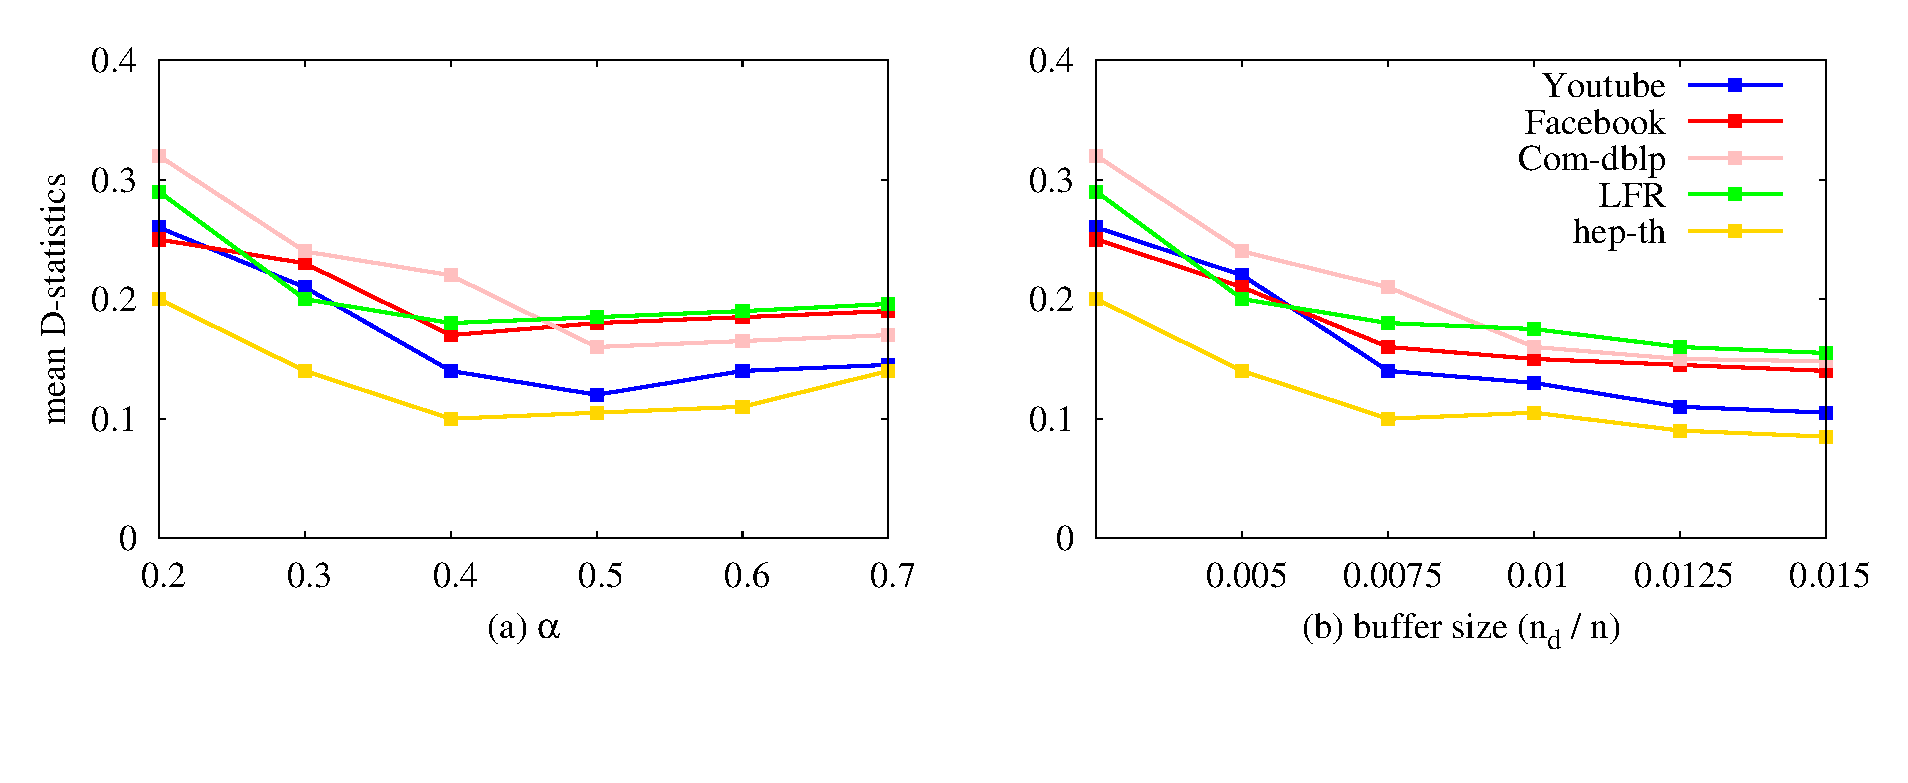
\includegraphics[width=0.8\columnwidth]{./texfiles/Chapter_2/figures/param_estimate.eps}
%\vspace{-12mm}
\caption{\label{param_est}Average $D$-statistics value across all the topological measures.}
\vspace{3mm}
%\vspace{-3mm}
\end{figure}


\iffalse
\begin{table}[!t]
\centering
\caption{\label{g_metric_alg}NMI between the ground-truth and community structure obtained from individual sampling algorithms for all datasets.}
%\scalebox{0.8}{
\begin{tabular}{l cccccc}
\hline
\multirow{1}{*}{{\bf Dataset}} & \multicolumn{1}{c}{{\bf \compas}} & \multicolumn{1}{c}{{\bf SN}} & \multicolumn{1}{c}{{\bf SE}} & \multicolumn{1}{c}{{\bf SBFS}} & \multicolumn{1}{c}{{\bf PIES}} & \multicolumn{1}{c}{{\bf GA}} \\\hline
Facebook	  & 0.52 & 0.34 & 0.28&0.41&0.48&0.61\\
hep-th		  &0.51&0.32&0.21&0.36&0.39&0.68\\
Youtube		      &0.72&0.49&0.33&0.58&0.51&0.77 \\
dblp		  &0.65&0.28&0.21&0.57&0.39&0.69 \\
LFR		  &0.69&0.29&0.32&0.38&0.31&0.72\\\hline
Average & {\bf 0.61}  & 0.34 & 0.27 & 0.46  & 0.41 & {\bf 0.69}    \\
\hline
\end{tabular}
%\vspace{4mm}
\end{table}
\fi
\begin{table}[!t]
\centering
\caption{\label{g_metric_alg}Purity (PU), NMI and ARI values between the ground-truth and community structure obtained from individual sampling algorithms for all datasets.}
\scalebox{0.68}{
\begin{tabular}{l |>{\columncolor[gray]{0.8}} c>{\columncolor[gray]{0.8}}  c>{\columncolor[gray]{0.8}}  c|  c  c  c| ccc|ccc|ccc|>{\columncolor[gray]{0.8}}c>{\columncolor[gray]{0.8}}c>{\columncolor[gray]{0.8}}c}
\hline
\multirow{2}{*}{{\bf Dataset}} & \multicolumn{3}{c|}{{\bf \compas}} & \multicolumn{3}{c|}{{\bf SN}} & \multicolumn{3}{c|}{{\bf SE}} & \multicolumn{3}{c|}{{\bf SBFS}} & \multicolumn{3}{c|}{{\bf PIES}} & \multicolumn{3}{c}{{\bf GA}} \\\cline{2-19}
   & \multicolumn{1}{c}{PU} & \multicolumn{1}{c}{NMI} & \multicolumn{1}{c|}{ARI} & PU & NMI & ARI &PU & NMI & ARI &PU & NMI & ARI &PU & NMI & ARI & \multicolumn{1}{c}{PU} & \multicolumn{1}{c}{NMI} & \multicolumn{1}{c}{ARI} \\\hline
Facebook	  & 0.71 & 0.52 & 0.47	 & 0.43&0.34&0.26  & 0.39&0.28&0.12  &  0.53&0.41&0.18  & 0.57&0.48&0.36  & 0.76&0.61&0.52 \\
hep-th		  &	0.69&0.51&0.38 & 0.39&0.32&0.19 & 0.29&0.21&0.12 & 0.42&0.36&0.25  & 0.48&0.39&0.31 & 0.74&0.68&0.57\\
youtube		      & 0.83&0.72&0.67	 &  0.52&0.49&0.36 & 0.48&0.33&0.28  &  0.63&0.58&0.47 & 0.56&0.51&0.41  & 0.86&0.77&0.71 \\
Dblp		  &	0.72&0.65&0.58 & 0.32&0.28&0.21  & 0.29&0.21&0.16  & 0.66&0.57&0.32  & 0.48&0.39&0.31  & 0.79&0.69&0.52 \\
LFR		  & 0.76&0.69&0.55	 & 0.35&0.29&0.21  & 0.56&0.32&0.29  & 0.49&0.38&0.26  & 0.42&0.31&0.28  &  0.81&0.72&0.67 \\\hline
Average & 0.74 & 0.61 & 0.53 & 0.40 & 0.34 & 0.24 & 0.40 & 0.27 &0.19 & 0.54 & 0.46 & 0.29 & 0.50 & 0.41 & 0.33 & 0.79 & 0.69 & 0.59   \\
\hline
\end{tabular}}
\vspace{3mm}
\end{table}


 {\bf Comparison of sampling algorithms}:
We start by measuring the similarity between the obtained and the ground-truth community structures using topological measures. In tables \ref{tab_fb},  \ref{tab_hep-th}, \ref{tab_yt}, \ref{tab_dblp} and \ref{tab_lfr} 
we summarize the $D$-statistics values of all the scoring functions for Facebook, arxiv hep-th, Youtube, dblp and LFR datasets respectively. 
%for the other graphs we only present the average value (and standard deviation) across the $D$-statistics for different topological 
%measures (detailed results on other datasets can be accessed in  \cite{si}). 
\iffalse\TODO{For these networks we MUST report standard deviation/error}.\fi 
Clearly~\compas~outperforms all the streaming algorithms across different datasets. GA performs better than~\compas~since it has in its 
consideration the whole graph to obtain the sample. However, we stress that even with {\em minimal community information to start with} and 
{\em no subsequent community detection in the later steps}, we are able to reach very close to GA as well as to the ground-truth.

Further we find \compas~is the second ranked algorithm after GA with an average 
(over all datasets) purity, NMI and ARI of {\bf 0.74}, {\bf 0.61} and {\bf 0.53} respectively (see table \ref{g_metric_alg} for detailed results). 
%(see Table \ref{g_metric_alg}  for NMI, details in \cite{si}).
\iffalse As a second level of evaluation, we further calculate three validation metrics -- purity, NMI and ARI  between the ground-truth and the obtained community structure for all the algorithms . Once again we observe that \\ \fi

\noindent{\bf Effect of edge ordering and sample size:}\label{sec:effect}
In this section, we show that most of our inferences are valid irrespective of any edge ordering. We randomly pick one pair of edges and swap their arrival time. 
We repeat it for $y$\% of edges (where $y$ varies between 5 and (as high as) 50) present in each aggregated graph. %\textcolor{red}{Put results starting from $x=5$ in steps of 5 up to 50.} 
%Each value of $x$ represents a new ordering with a higher value representing higher disorder. 
For each such ordering we obtain a representative sample (say $G_y$) and compare (average $D$-statistics)  with 
the ground-truth community. 
%the original graph ($S$). obtained considering the original arrival 
%order. The comparison is done by obtaining the distribution of each community scoring function for $S_x$ and $S$ and, subsequently, calculating the $D$-statistics.  
%For each value of $x$, we compare (through $D$-statistics) the distribution of each scoring function with the original order of edge arrivals. 
In figure~\ref{param_est_1}(a) we plot the $D$-statistics value averaged over all the scoring functions for the Youtube dataset. The plot clearly shows that the edge-ordering  
affects the final sample marginally.
%shows that for the Youtube graph edge ordering does not affect the final sample much (the pattern is same for LFR graph, see \cite{si}).
%\TODO{Mention how you obtained the ordering each time? Is it different random order or is there some strategic order also. You should make it explicit and say that~\compas~is tolerant to only these orders. DONE} 
%\textcolor{blue}{To obtain arrival sequences we consider two edges and swap their arrival times. This we do for 20\% of the total edges in the original network.

Lastly, we present the effect of sample size ($n$) on the obtained community structure. We plot average $D$-statistics values across all the topological measures for all the algorithms on Youtube as a function of $n$ (figure \ref{param_est_1}(b)). As expected, with the increase of $n$ we obtain better results. Interestingly, for~\compas~and GA, the pattern remains consistent compared to others. Moreover as we increase $n$ the divergence between their performance decreases.

%\vspace{-3mm}
\begin{figure}[!h]
\centering
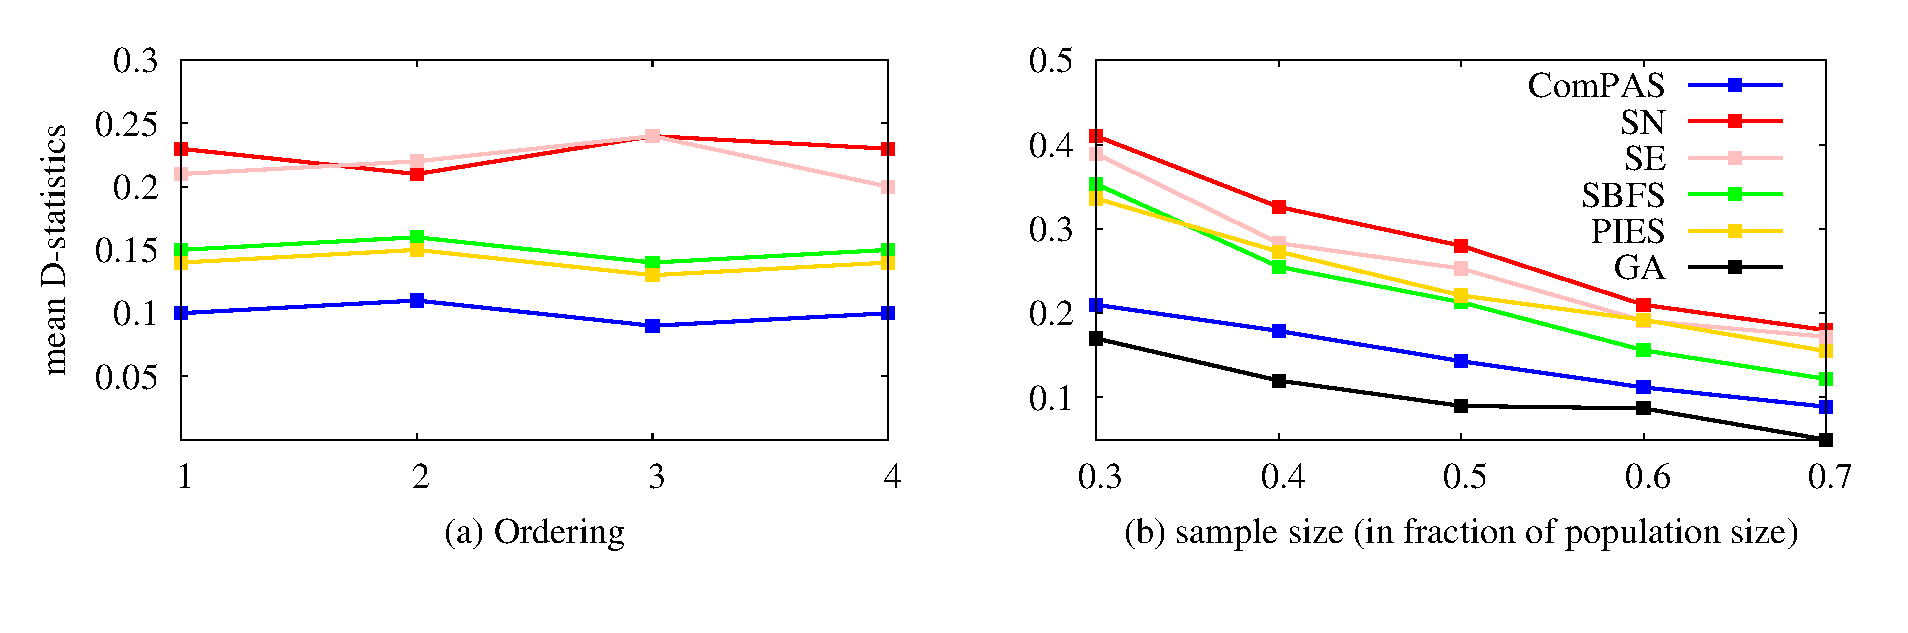
\includegraphics[width=0.8\columnwidth]{./texfiles/Chapter_2/figures/param_estimate_1.eps}
%\vspace{-10mm}
\caption{\label{param_est_1}Average $D$-statistics across all the topological measures for (a) different edge ordering and (b) sample size ($n$) of the Youtube graph.}
\vspace{4mm}
\end{figure}






%%%%%%%%%%%%%%%%%%%%%%%%%%%%%%%%%%%%%%%%%%%%%%%%%%%%%%%%%%%%%%%%%%%
\if{0}
{\bf Comment on edge-density of the sample}: 
Note that \compas~ is node-based, i.e., sample size is controlled by the number of nodes, and we at any point do not limit the number of edges in the sample ($e_{s}$). We compare the number of edges in the sample against that in the subgraph induced by the nodes in the obtained sample ($e_{p}$). 
We observe that on average our sample consists of only $\sim71$\% of the edges in the induced subgraph across all the datasets. 
%\iffalse\TODO{Sandipan: I had initially added a plot but decided against putting it as I felt it was not providing any extra information.}\fi
%which is followed by SBFS, PIES, SN and SE.
\iffalse
\subsection{Graph-centric evaluation}
\label{graph_evaluation}
We further evaluate our sample in terms of three graph properties mentioned in \cite{ahmed2014network}: (i) degree distribution (Degree), (ii) clustering coefficient distribution (CC), (iii) top 100 eigen value distribution (EV). 
Table \ref{graph_prop} reports the $D$-statistics values between the distributions of the original graph and those obtained from the sample (see more results in \cite{si}). For all the datasets, we observe that \compas~is within top three ranks in terms of low $D$-statistics, in many cases, also beating the strict baseline GA. This indicates that \compas~ also preserves general graphs properties in the sample.

\vspace{-2mm}
\begin{table}[!h]
\centering
\caption{Summary of $D$-statistics for different graph properties. For Youtube we present all the results, while for the rest we provide only average $D$-statistics (top three results in each average case are highlighted).}
\label{graph_prop}
\begin{adjustbox}{max width=\columnwidth}
\begin{tabular}{l|c c c |c|c|c|c|c}
\hline
  \multirow{2}{*}{Algorithm}         & \multicolumn{4}{c|}{Youtube}     & Facebook & Com-dblp & LFR     & hep-th  \\ \cline{2-9}
& Degree & CC & EV & Average & Average  & Average  & Average & Avearge \\ \hline
\compas    &   0.083     & 0.105   & 0.42     &  {\bf 0.20}       &  {\bf 0.17}        &  {\bf 0.16}       & {\bf 0.28}        & {\bf 0.18}       \\ 
SN        &    0.076    & 0.108   &  0.54     &  0.24             &   0.36             &  0.24             & 0.34              &  0.23       \\ 
SE        &    0.114    & 0.195   &  0.39     &  0.23             &   0.48             &  0.28             & 0.39              &  0.27       \\ 
SBFS      &    0.105    & 0.172   &  0.32     &  {\bf 0.19}       &   {\bf 0.28}       &  {\bf 0.13}       & {\bf 0.26}        & {\bf 0.19}       \\ 
PIES      &    0.046    &  0.129  &  0.38     &  {\bf 0.18}       &   {\bf 0.16}       &  0.21             & {\bf 0.28}        & {\bf 0.16}        \\ 
GA        &    0.218    &  0.063  &  0.46     &  0.24            &   0.35             &  {\bf 0.12}       & 0.32              &  0.20       \\ \hline
\end{tabular}
\end{adjustbox}
\vspace{-1mm}
\end{table}
\fi
%\vspace{-2mm} 

{\bf Effect of edge ordering and sample size:}
In this section, we show that most of our inferences are valid irrespective of any edge ordering. To do so, we randomly pick one pair of edges and swap their arrival time. 
We repeat it for $x$\% of edges (where $x$ varies between 5 and 50) present in each aggregated graph. %\textcolor{red}{Put results starting from $x=5$ in steps of 5 up to 50.} 
Each value of $x$ represents a new ordering with a higher 
value representing higher disorder. For each such ordering we obtain a representative sample (say $S_x$) and compare with sample ($S$) obtained considering original arrival 
order. The comparison is done by obtaining the distribution of each community scoring function for $S_x$ and $S$ and thereby calculating the $D$-statistics.  
%For each value of $x$, we compare (through $D$-statistics) the distribution of each scoring function with the original order of edge arrivals. 
In figure \ref{param_est_1}(a) we plot the $D$-statistics value averaged over all the scoring functions for Youtube dataset. 
The plot clearly shows that edge-ordering does not 
affect the final sample much. 
%(the pattern is same for LFR graph, see \cite{si}).
%\TODO{Mention how you obtained the ordering each time? Is it different random order or is there some strategic order also. You should make it explicit and say that~\compas~is tolerant to only these orders. DONE} 
%\textcolor{blue}{To obtain arrival sequences we consider two edges and swap their arrival times. This we do for 20\% of the total edges in the original network.
Lastly, we present the effect of sample size ($n$) on the obtained community structure. We plot average $D$-statistics values across all the topological measures for all the algorithms on Youtube  (see others in \cite{si}) as a function of $n$ (Figure \ref{param_est_1}(b)). As expected, with the increase of $n$ we obtain better results. Interestingly, for~\compas~and GA, the pattern remains consistent compared to others.\\


\noindent{\bf Extensions:} In its current form, our algorithm is applicable to undirected and and unweighted networks. We believe that through minor modifications our algorithm could be extended to 
directed as well as as weighted networks. \compas~ is aimed at optimizing modularity which has already been precisely defined for weighted~\cite{newman2004analysis} and 
directed networks~\cite{leicht2008community}. Further, the same sub-routines in the original algorithm, with minor modifications could be used for directed and weighted networks. 
The theoretical analysis would require additional research efforts which we plan to take up in future.

%\vspace{-5mm}
\begin{figure}[!h]
\centering
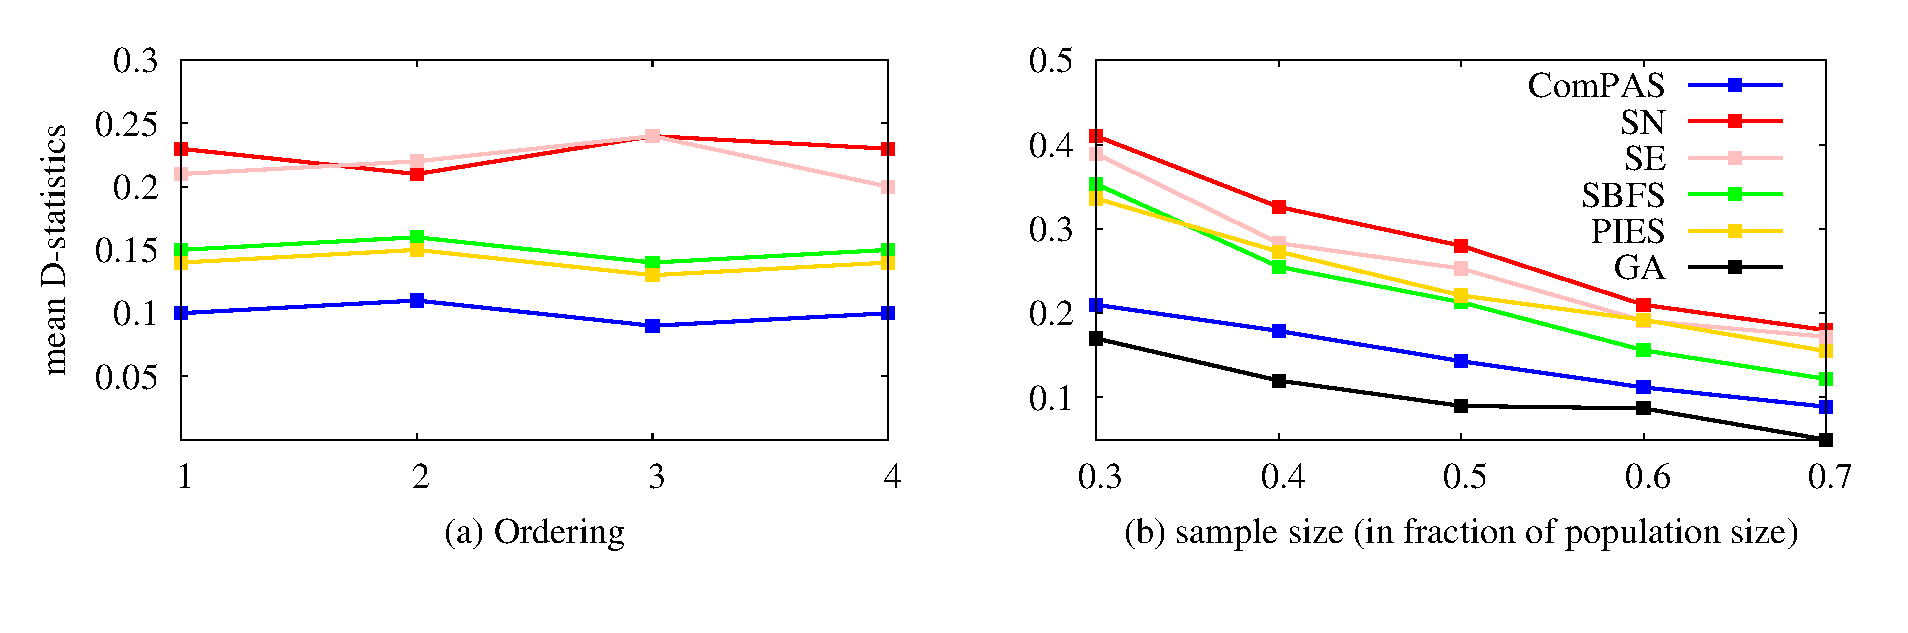
\includegraphics[width=0.8\columnwidth]{./texfiles/Chapter_2/figures/param_estimate_1.eps}
%\vspace{-10mm}
\caption{\label{param_est_1}Average $D$-statistics across all the topological measures for (a) different edge ordering and (b) sample size ($n$) of the Youtube graph.}
\vspace{4mm}
\end{figure}
\fi



%\if{0}

%\fi






\input{./texfiles/Chapter_2/complexity}
%\section{Applications of compas}
Here we present two additional applications of \compas~-- ranking community detection algorithms, and selecting appropriate training set for (restricted) online learning. 
\subsection{Ranking community detection algorithms} As pointed out in \cite{maiya2010sampling}, there is always a trade-off between quality and running time for discovering the community structure from a graph. While some algorithms discover excellent community structure with larger running time, others compromise  quality by achieving lesser running time. Further, it is not possible to identify beforehand which community detection algorithm is more useful given a large graph. In this case, one is forced to run several algorithms on the large graph and converge on the best performing one. This may lead to a large computation cost and is especially detrimental in resource-scarce situations (absence of parallel infrastructures, distributed systems etc.).

In case of community detection on large streaming graphs, we 
posit that one may first execute \compas~and obtain a community-preserved sample. Then different community detection algorithms can be tested on the sample (which is much smaller in size compared to the original graph) and the best performing algorithm can be used for the original large graph. To this end, we execute five community detection (CD) algorithms (CNM \cite{clauset2004finding}, Fast-Greedy \cite{newman2004fast}, Walktrap \cite{pons2005computing}, Infomod \cite{rosvall2007information}, Infomop \cite{rosvall2008maps}) separately on each sample obtained from the sampling algorithms. Then we rank the CD algorithms based on their performance in terms of  modularity~\cite{newman2004analysis}. We further rank the CD algorithms in the same way considering the {\em entire graph}. We report the Kendall's $\tau$ rank correlation in Table~\ref{comp_wiki}(a) between these two ranks for individual sampling algorithms across all the datasets. We find GA and \compas~ performing the best. Therefore, \compas~can be used for selecting a CD algorithm quickly before running on a large streaming graph.

%This leads us to believe sample obtained through \compas~correctly ranks the performance of the community detection algorithms. 





\begin{table}[!t]
\centering
\caption{\label{comp_wiki} Rank correlation of community detection algorithms based on the performance on the sample (generated from individual sampling methods) and the original graph. (b) Performance of SVM using the training set obtained from sampling methods.}
\scalebox{0.71}{
\begin{tabular}{|c|c|c|c|c|c|c |c|c|}
\multicolumn{6}{c}{(a)} & \multicolumn{1}{c}{} & \multicolumn{2}{c}{(b)}\\ \cline{1-6}\cline{8-9}
Algo & Facebook & hep-th & Youtube & DBLP & LFR & &AUC & F-Score \\\cline{1-6}\cline{8-9}

\compas & {\bf 0.8} & {\bf 0.8} & {\bf 0.8} & {\bf 1.0} & {\bf 1.0}& & {\bf 0.48} & {\bf 0.61}  \\
SN & 0.4 & 0.6 & 0.4 &  0.6 & 0.6& & 0.31 & 0.35 \\
SE & 0.4 & 0.4& 0.4 &  0.6 & 0.4& & 0.25 & 0.28 \\
SBFS & 0.6 & 0.7 & 0.6 & 0.8 & 0.6& & 0.28 & 0.31 \\
PIES & 0.6 & 0.6 & 0.8 & 0.7 & 0.8& & 0.36 & 0.43\\
GA   & {\bf 1.0} & {\bf 0.8} & {\bf 0.8} & {\bf 1.0} & {\bf 1.0} & & {\bf 0.53} & {\bf 0.64} \\\cline{1-6}\cline{8-9}
\end{tabular}}
\end{table}


\subsection{Selecting training set for online learning}

In online learning, sometimes memory is limited and it is required to train the model on limited number of instances. In such situations it is important to choose a training set in such a way that it consists of members from most or all parts of the original dataset.

We hypothesize that more diverse the chosen set, better would be the performance. \compas~ is useful in such cases since it tries to sample from several communities, hence improving the diversity of the training set. To this end, we consider Wiki-Rfa\footnote{https://snap.stanford.edu/data/wiki-RfA.html} \cite{west2014exploiting}, a streaming signed graph in which nodes represent Wikipedia members and edges (with time-stamp) represent votes. Each vote is typically accompanied by a short comment. The task is to predict the vote (+1, 0, -1) of an incoming edge based on the textual features -- (i) word count, (ii) sentiment value, and (iii) LIWC features of the statement corresponding to the edge. We allow training instances to be included till a certain time period $t$ (first 75\% of the edges are allowed to enter) and run the sampling algorithms in parallel. However not all instances can be considered for training due to the memory constraint. We assume $n$, the sample size as the allowed training size and obtain sampled training set from individual sampling algorithms. We train SVM with linear kernel (see \cite{si} for other classifiers) on each sampled training set, and predict the labels (votes) of those instances coming after $t$. Table \ref{comp_wiki}(b) shows that GA and \compas~perform the best in terms of AUC and F-Score. 
 This once again emphasizes the fact that \compas~selects most representative training instances for (restricted) online learning.
 



\section{Summary of the chapter}
The contributions of this chapter can be summarized as follows - 
\begin{itemize}
 \item We proposed \compas, a novel sampling algorithm for streaming graphs 
which is able to retain the community structure of the original graph.
 \item Through rigorous experimentation on four real-world and one synthetic graphs we showed that our algorithm performs better than 
five state-of-the-art graph sampling algorithms.
 \item We further showed the effectiveness of \compas~ in online learning frameworks
\end{itemize}
  
A possible future direction would be to analytically estimate the relation between sample size and the accuracy of our algorithm. 
It would also be interesting to investigate in detail the effectiveness of \compas~ in other real applications. 

%We also plan to check whether the present algorithm could be modified to estimate multiple graph properties. Finally we plan to extend our work to directed and weighted networks.  


%\appendix
%PROPOSITION 1.
{\em
For a community $c\in C$, if $D_c\leq M-1$ then addition of an edge within $c$ will increase its modularity.}

\begin{proof}
From Equation \ref{modularity}, we see the contribution of individual community $c\in C$ in modularity as: $Q_c=\frac{m_c}{M} - \frac{D_c^2}{4M^2}$. 
where $m_c$ is the number of edges inside $c$, $M$ is the total number of edges in the graph, and $D_c$ is the sum of degrees of all the nodes in $c$. 

Addition of a new edge within $c$, the $c$'s contribution of modularity becomes:
\[
Q'_c=\frac{m_c+1}{M+1} - \frac{(D_c+2)^2}{4(M+1)^2}
\]

So the increase in modularity is $\Delta Q_c=Q'_c-Q_c$,
\[\small
\begin{split}
\Delta Q_c=&\frac{4M^2-4m_cM^2-4D_cM^2-4m_cM+2D_c^2M+D_c^2}{4(M+1)^2M^2}\\
&\geq \frac{4M^2-6D_cM^2-2D_cM+2D_c^2M+D_c^2}{4(M+1)^2M^2}\\
&\geq\frac{(2M^2-2D_cM-D_c)(2M-D_c)}{4(M+1)^2M^2}\\
&\geq 0
\end{split}
\]
The equality holds if $D_c\leq M-1$. This thus implies $(2M^2-2D_cM-D_c)\geq 0$. This proves the proposition.
\end{proof}

PROPOSITION 2.
{\em For a community $c\in C$, addition of any intra-community edge into $c$ should not split it into smaller communities.}


\begin{proof}
We will prove this proposition by contradiction.
Assume that once a new intra-community edge is added into $c$, it gets split into $k$ small modules, namely $X_1$, $X_2$, $\cdot$,$X_k$. Let $D_{X_i}$ and $e_{ij}$ be the total degree of nodes inside $X_i$ and number of edges connecting $X_i$ and $X_j$ respectively. 


Recall that the contribution of $X_i$ in the modularity value is $Q_{X_i}=\frac{m_{X_i}}{M} - \frac{D_{X_i}^2}{4M^2}$.  Before adding the edge, we have $Q_c \geq \sum_{i=1}^k Q_{X_i}$ (where $Q_c$ is the total modularity of community $c$), because otherwise all $X_i$s can be split earlier, which is not in this case. This implies that:
\[
\frac{m_c}{M}- \frac{D_c^2}{4M^2} > \sum_{i=1}^k (\frac{m_{X_i}}{M} - \frac{D_{X_i}^2}{4M^2})
\]
Since $X_1,X_2,\cdot,X_k$ are all disjoint modules of $c$, $D_c=\sum_{i=1}^k D_{X_i}$ and $m_c=\sum_{i=1}^k m_{X_i} + \sum_{i<j} e_{ij}$. This further implies that:
\[
\frac{m_c}{M}-\sum_{i=1}^k \frac{m_{X_i}}{M} > \frac{D_c^2}{4M^2}- \sum_{i=1}^k \frac{D_{X_i}^2}{4M^2}
\]
or,
\[
\sum_{i<j} e_{ij} > \frac{\sum_{i<j} D_{X_i}D_{X_j}}{2M}
\]
 
 Without loss of generality, let us assume that the new edge is added inside $X_1$. 
Since we assume that after adding the new edge into $c$, it gets split into $k$ small modules, the modularity value should increase because of the split. Therefore, the new modularity $Q'_c<\sum_{i=1}^k Q_{X_i}$. This implies that
\[\small
\begin{split}\small
& Q'_c < \sum_{i=1}^k Q_{X_i}\\
& \Leftrightarrow \frac{\sum_{i=1}^k m_{X_i} + \sum_{i<j} e_{ij} + 1}{M+1} - \frac{(\sum_{i=1}^k D_{X_i +2})^2}{4(M+1)^2}\\
& <  \frac{m_{X_1}+1}{M+1} - \frac{(D_{X_1}+2)^2}{4(M+1)^2}  + \sum_{i=2}^k  (\frac{m_{X_i}}{M+1} - \frac{D_{X_i}^2}{4(M+1)^2} )\\
&\Leftrightarrow \frac{\sum_{i=1}^k m_{X_i} + \sum_{i<j} e_{ij} + 1}{M+1} - \frac{(\sum_{i=1}^k D_{X_i +2})^2}{4(M+1)^2}\\
& < \frac{\sum_{i=1}^k m_{X_i}+1}{M+1} - \frac{(D_{X_1}+2)^2}{4(M+1)^2} - \sum_{i=2}^k \frac{D_{X_i}^2}{4(M+1)^2}\\
&\Leftrightarrow \sum_{i<i} e_{ij} < \frac{\sum_{i=1}^k D_{X_i} - 2 D_{X_1} + \sum_{i<j} D_{X_i}D_{X_j}}{2(M+1)}
\end{split}
\]
Since $\sum_{i=1}^k D_{X_i} - 2D_{X_1} < 2M$, this implies that 
\[\small
\begin{split}
\frac{\sum_{i<j}D_{X_i}D_{X_j}}{2M}  < \sum_{i<j}e_{ij} 
&< \frac{\sum_{i=1}^k D_{X_i} - 2D_{X_1} + \sum_{i\neq j}{D_{X_i}D_{X_j}}}{2(M+1)}\\
& <\frac{\sum_{i<j}D_{X_i}D_{X_j}}{2M}+1
\end{split}
\]
Therefore, the proposition holds.
\end{proof}





PROPOSITION 3.
{\em If a new edge $(u,v)$ connecting two communities $C(u)$ and $C(v)$ is introduced, $C(u)$ $($or $C(v))$ is the best candidate for $v$ (or $u$) if it should ever change its community membership.}

\begin{proof}
The method is inspired by \cite{PhysRevE.78.046115} that a vertex $u$ is influenced by two factors: $F^c_{in}(u)$ the force that keeps $u$ stay in its own community $c$, and $F^c_{out}(u)$, the force that a community $S$ imposes to $u$ in order to bring $u$ to $S$ as follows:
\[
F^c_{in}(u)=e_c^u-\frac{d_u(D_c-d_u)}{2M}
\]
and 
\[
F^S_{out}(u)=max_{S\in NC(u)} \{e_S^u - \frac{d_u D_{outS}}{2M}\}
\]
where $NC(u)$ is the set of neighboring communities of $u$, and $D_{outS}$ is the total degree of vertices outside $S$.

Now we will show that the presence of new edge $(u,v)$ will strengthen $F^{C(v)}_{out}(u)$ and weaken $F^S_{out}(u)$. In other words, we will show that $F^{C(v)}_{out}(u)$ increases while $F^S_{out}(u)$ decreases for all $S \in C \wedge S \notin \{C(u),C(v)\}$.
\[\small
\begin{split}
&F^{C(v)}_{out}(u)|_{new} - F^{C(v)}_{out}(u)|_{old}\\
&=(e_u^{C(v)}+1-\frac{(d_u+1)(d_{outC(v)}+1)}{2(M+1)} - (e_u^{C(v)} - \frac{d_ud_{outC(v)}}{2M})\\
&= \frac{2M+d_ud_{outC(v)}}{2(M+1)} - \frac{d_ud_{outC(v)}+d_{outD(v)}+d_u+1}{2(M+1)}\\
&\geq \frac{2M+d_ud_{outC(v)}}{2(M+1)} - \frac{d_u d_{outC(v)}+d_{outC(v)}+d_u+1}{2(M+1)}\\
&>0
\end{split}
\]
Therefore $F^{C(v)}_{out}(u)$ is strengthen when new edge $(u,v)$ is introduced. Furthermore, for any community $S\in C \wedge S\notin \{C(u),C(v)\}$
\[
\begin{split}
& F^{S}_{out}(u)|_{new} - F^{S}_{out}(u)|_{old}\\
&= (e^S_u-\frac{(d_u+1)d_{outS}}{2(M+1)}) - (e^S_u - \frac{d_ud_{outS}}{2M})\\
&= d_{outS}(\frac{d_u}{2M} - \frac{d_u+1}{2(M+1)})<0
\end{split}
\]

This implies that $F^S_{out}(u)$ is weakened when $(u,v)$ is added. Therefore,  the proposition holds.
\end{proof}


PROPOSITION 4.
{\em If a new edge $(u,v)$ is added into the network, then joining $u$ to $v$'s $C(v)$ community will increase the modularity value  if $\Delta Q(u,C(u),C(v)) \equiv 4(M+1)(e_{C(v)}^u+1-e_{C(u)}^u)+e_{C(v)}^u(2D_{C(v)}-2d_u-e_{C(u)}^u) - 2(d_u+1)(d_u+1+d_{C(v)}-d_{C(u)})>0$.}

\begin{proof}
Vertex $u$ will leave its current community $C(u)$ and join $v$'s community $C(v)$ if\\
\[\scriptsize
\begin{split}
& Q_{C(v)+u} + Q_{C(u)-u} > Q_{c(u)} + Q_{C(v)}\\
&\Leftrightarrow \frac{m_{C(v)}+e_{C(v)}+1}{M+1} - \frac{(d_{C(v)}+d_u+2)^2}{4(M+1)^2}+\\
&\frac{m_{C(u)} - e_{C(u)}}{M+1} - \frac{(d_{C(u)}-d_u-e_{C(u)})}{4(M+1)^2} \\
& > \frac{m_{C(v)}}{M+1} - \frac{(d_{C(v)}+d_u+2)^2}{4(M+1)^2} + \frac{m_{C(u)}}{M+1} - \frac{(d_{C(u)}+1)^2}{4(M+1)^2}\\
&\Leftrightarrow 4(M+1)(e_{C(v)} +1 -e_{C(u)}) + e_{C(u)}(2d_{C(v)} - 2d_{C(u)}-e_{C(u)})\\
& - 2(d_{C(u)}+1)(d_{C(u)}+1+d_{C(v)}-d_{C(u)})>0
\end{split}\]
\end{proof}


\newpage
%\bibliographystyle{abbrv}
%\bibliography{sigproc} 
%\end{document}



\clearpage
\clearpage


%\documentclass[doublecol]{epl2} 
% or \documentclass[page-classic]{epl2} for one column style

% \usepackage{amsfonts}
% \usepackage{graphicx}
% \usepackage{url}
% \usepackage{float}
% \usepackage{latexsym}
% \usepackage{amsmath,amssymb}
% \usepackage{dcolumn}
% \usepackage{epsfig}
% \usepackage{textcomp}
% \usepackage{mathtools}
% \usepackage{multirow}
% \usepackage{algorithm}
% \usepackage{algorithmic}
% \usepackage{soul}
% \usepackage{color}
% \usepackage{amsmath}
% \usepackage{adjustbox}
%\newcommand{\todo}[1]{\textcolor{red}{TODO: #1}}

\setcounter{MaxMatrixCols}{10}
%TCIDATA{OutputFilter=Latex.dll}
%TCIDATA{Version=5.00.0.2606}
%TCIDATA{<META NAME="SaveForMode" CONTENT="1">}
%TCIDATA{BibliographyScheme=BibTeX}
%TCIDATA{LastRevised=Sunday, February 28, 2016 13:36:09}
%TCIDATA{<META NAME="GraphicsSave" CONTENT="32">}
%TCIDATA{Language=American English}

\newtheorem{theorem}{Theorem}
\newtheorem{acknowledgement}[theorem]{Acknowledgement}
\newtheorem{axiom}[theorem]{Axiom}
\newtheorem{claim}[theorem]{Claim}
\newtheorem{conclusion}[theorem]{Conclusion}
\newtheorem{condition}[theorem]{Condition}
\newtheorem{conjecture}[theorem]{Conjecture}
\newtheorem{corollary}[theorem]{Corollary}
\newtheorem{criterion}[theorem]{Criterion}
\newtheorem{definition}[theorem]{Definition}
\newtheorem{example}[theorem]{Example}
\newtheorem{exercise}[theorem]{Exercise}
\newtheorem{lemma}[theorem]{Lemma}
\newtheorem{notation}[theorem]{Notation}
\newtheorem{problem}[theorem]{Problem}
\newtheorem{proposition}[theorem]{Proposition}
\newtheorem{remark}[theorem]{Remark}
\newtheorem{solution}[theorem]{Solution}
\newtheorem{summary}[theorem]{Summary}
\def\dint{\mathop{\displaystyle \int}}
\def\diint{\mathop{\displaystyle \iint }}
\def\diiint{\mathop{\displaystyle \iiint }}
\def\diiiint{\mathop{\displaystyle \iiiint }}
\def\didotsint{\mathop{\displaystyle \idotsint }}
\def\doint{\mathop{\displaystyle \oint}}
\def\dsum{\mathop{\displaystyle \sum }}
\def\dprod{\mathop{\displaystyle \prod }}
\def\dbigcap{\mathop{\displaystyle \bigcap }}
\def\dbigwedge{\mathop{\displaystyle \bigwedge }}
\def\dbigoplus{\mathop{\displaystyle \bigoplus }}
\def\dbigodot{\mathop{\displaystyle \bigodot }}
\def\dbigsqcup{\mathop{\displaystyle \bigsqcup }}
\def\dcoprod{\mathop{\displaystyle \coprod }}
\def\dbigcup{\mathop{\displaystyle \bigcup }}
\def\dbigvee{\mathop{\displaystyle \bigvee }}
\def\dbigotimes{\mathop{\displaystyle \bigotimes }}
\def\dbiguplus{\mathop{\displaystyle \biguplus }}
\def\BF#1{{\bf {#1}}}
\def\NEG#1{\leavevmode\hbox{\rlap{\thinspace/}{$#1$}}}



% \title{Threshold-based epidemic dynamics in systems with memory}
% \shorttitle{Threshold-based epidemic} %Insert here a short version of the title if it exceeds 70 characters
% 
% \author{Marcin Bodych\inst{2}, Niloy Ganguly\inst{1}, Tyll Krueger\inst{2}, Animesh Mukherjee\inst{1}, Rainer Siegmund-Schultze\inst{3} \and Sandipan Sikdar\inst{1}}
% \shortauthor{M. Bodych \etal}
% 
% \institute{                    
%   \inst{1} Indian Institute of Technology Kharagpur - Kharagpur, India - 721302\\
%   \inst{2} Wroclaw University of Technology - 27 50-370 Wrocław, Poland \\
%   \inst{3} Technical University Berlin - 10623 Berlin, Germany
% }
% \pacs{89.75.Hc}{First pacs description}
% \pacs{89.75.Fb}{Second pacs description}
%\pacs{nn.mm.xx}{Third pacs description}


% \abstract{
% In this article we analyze an epidemic dynamics model (SI) where 
% we assume that there are $k$ susceptible states, that is a node would require multiple ($k$) contacts before it gets infected. 
% In specific, we provide a theoretical framework for studying diffusion rate in 
% complete graphs and $d$-regular trees with extensions to dense random graphs. We observe that irrespective of the topology, the diffusion process could be 
% divided into two distinct phases: (i) the {\em initial} phase, where the diffusion process is slow, followed by (ii) {\em residual} phase where the diffusion rate 
% increases manifold. In fact, the initial phase acts as an indicator for the total diffusion time in dense graphs. 
% The most remarkable lesson from this investigation is that such a diffusion process {\em could be controlled and even contained if acted upon within its initial phase}.}
% 
% 
% \begin{document}
% 
% \maketitle


% \section{Section title}
% Insert here the text.
% See fig.~\ref{fig.1}, table~\ref{tab.1} and eq.~(\ref{eq.1}).
% See also~\cite{b.a,b.b}.
% \begin{equation}
% \label{eq.1}
% 0\neq1
% \end{equation}
% 
% 
% \begin{figure}
% \onefigure{epl-template.eps}
% \caption{Figure caption.}
% \label{fig.1}
% \end{figure}
% 
% 
% \begin{table}
% \caption{Table caption.}
% \label{tab.1}
% \begin{center}
% \begin{tabular}{lcr}
% first  & table & row\\
% second & table & row
% \end{tabular}
% \end{center}
% \end{table}
\chapter{Diffusion in temporal networks}
Previous two chapters dealt with analyzing structural properties of temporal networks. This chapter is devoted toward the functional aspect of time-varying networks.  
In specific, we are interested in studying diffusion dynamics in these networks. 
This chapter is divided into two parts. To start with we propose a threshold based diffusion model and systematically analyze the diffusion rate for different underlying 
graph topologies. We then leverage these results to obtain a message broadcast algorithm in dynamic networks. 


\noindent
\section{Introduction}
Information diffusion is one of the most common phenomena that occurs on a
network and the most elementary model of this process is SI
(Susceptible-Infected)~\cite{anderson1992infectious} and its different variations~\cite{watts2002simple,dodds2004universal,pnas1,pnas2,tang2009epidemic,son2012percolation}.
Epidemic/adoption models have recently found a renewed interest with the formulation of temporal networks and 
realization that most of the real-world networks are temporal in nature (network structure changes with time). 
\if{0}
For example,  Takaguchi et. al. in~\cite{takaguchi2013bursty} presents a model whereby adoption behavior 
of a node is driven by the number of recent contacts with already adopted individual. 
Through simulations on real-world temporal networks the authors further show that burstiness~\cite{karsai2011small} 
affects spreading rate. Similar empirical study was also performed by Karimi et. al. in~\cite{karimi2013threshold}. A further modification to the 
model has been proposed by Backlund et. al. in~\cite{backlund2014effects} which considers that adoption is driven by the number of contacts
with different adopted neighbors within a chosen time instead of a particular neighbor multiple times. Further, information diffusion on temporal 
networks, more specifically prevalence, have also been studied in \cite{rocha2013bursts}. 
Several other results on the study of 
epidemics in temporal networks are listed in~\cite{masuda2013predicting} and on epidemic thresholds in~\cite{prl1,van2012epidemic,zhang2014susceptible}.
This type of history-dependent thresholding spreading pattern is largely observed in spread of bacterial diseases such as tuberculosis and 
dysentery \cite{joh2009dynamics} and 
also in peer-to-peer \cite{sanghavi2007gossiping} and Bittorrent systems \cite{qiu2004modeling}. In \cite{romero2011differences} the authors show that people 
accept ideas/news after repeated exposure.
\fi

The fundamental difference between static and temporal epidemic (SI) models is that in temporal models every agent  within a population is {\em not equally susceptible} to a disease or equally amenable to a rumor
 - the one which has been exposed more number of times (in recent past) are more amenable. This difference however is not well formulated and hence not well modeled - the primary contribution of this work 
is to succinctly define the problem in  terms of a simple model and then theoretically calculate the rate of spread of the epidemics. 
%Albeit a deep literature exists on the study of epidemics in temporal networks, they are mostly simulation based and to the best of our knowledge, a theoretical foundation on the topic is still wanting. 
We consider a spreading model in the lines of~\cite{takaguchi2013bursty} where each susceptible node needs to communicate with the 
infected nodes {\em multiple times} to contract infection. More importantly, unlike memoryless systems, we assume that each node comprises a memory which 
keeps track of the number of contacts it makes with infected ones. Note that in our system memory is a property which allows each node to remember the number 
of contacts it has already made with the infected ones. While Karimi et. al. studied the effect of burstiness in the diffusion process, we 
are more interested in estimating both empirically and analytically the diffusion time and rate.
Note that this model is completely different from  threshold models~\cite{granovetter1978threshold,sur1} where a node
 gets infected when majority of its neighbors are infected or probabilistic SI-models where an infected node,  on coming in contact, 
infects a susceptible node with a probability $p$,  as those are memoryless systems and the transition depends only on the activity of present time step. 
Our diffusion model also differs from the Neighborhood Exchange (NE) model proposed in \cite{volz2007susceptible}. NE assumes at any given time, an individual
will be in contact with an individual-specific number of neighbors with whom disease transmission is possible while our model considers that a node can be in contact with 
only a single individual. Also NE does not consider the fact that multiple contacts are required to contract infection.

The analytical results are obtained 
considering simple yet important topologies like the complete graph and the infinite $d$-regular trees which accounts for two extreme variants of network topology in terms of edge 
density. 
We demonstrate that the total diffusion time required for complemete graph topology (with $n$ nodes) scales as $n^{\frac{k-1}{k}}$ where $k>1$ is the number 
of contacts required to infect a susceptible individual. 
This is in sharp contrast to the case with $k$ = $1$, where it has been shown that diffusion time 
scales as $\log{(n)}$ ~\cite{rumarSreadingPushPull,rumourSpreading_evolvingGraph_PushPull}.
Another important inference we draw from the theoretical analysis is that irrespective of the topology the diffusion process could be divided into two phases: (i) an initial phase where the diffusion rate is very slow and 
(ii) a residual phase where the diffusion becomes very fast.
This inference is also a crucial contribution of this work which can help in containing 
the spread of infectious diseases with minimum overhead if acted upon in the initial phase which we further prove through a detailed empirical study.


\medskip

\noindent
{\bf Broadcast algorithm based on diffusion model:} The study of broadcast over unstructured and mobile networks always assumes that the 
size of the message is  small enough to be transfered from one node to other 
on the short durations of contacts between the nodes. 
Contrary to this, we here explore
 the idea of ``segmented messages'' where we assume that the duration of a contact 
between the nodes is not always sufficient for the transfer and therefore the message might need to be 
segmented/divided into sub-parts and sent individually. 
At the ethernet level such techniques of segmented broadcast are often termed as pipelined broadcast 
~\cite{patarasuk2008techniques, watts1995pipelined}. Note that this is equivalent to diffusion model we proposed earlier with number of contacts ($k$) replaced by number 
of packets in a message. 
We systematically study the effect of the size and partition structure of the message on the broadcast time.
 %considering different variants of the basic push-pull transfer protocol. 
% \textcolor{red}{Note that we essentially deal with a theoretical abstraction of the problem of segmented message spreading and show that it is 
% significantly different from the classical epidemic spreading.}{\bf we have not shown this.} \todo{Have we shown this?}
%The transmission algorithms that we propose might require suitable adjustments when it is adapted for a specific type of a dynamic network.      

%\todo{The two paragraphs need to be discussed, n, m, k, s are extremely confusing and need to be simplified}
{In specific, we investigate in details the effect of message segmentation as well as the message transfer protocols on the overall 
broadcast delay and message wastage. 
We assume that a big file is split into $k$ ($>1$) packets and 
%the packets are grouped into $s$ ($\geq 1$) segments, each containing $k$ packets. 
at the beginning, there is only one sender node in the network that has all the packets. 
Further, a node can transfer only one  packet in a single contact opportunity, and it can do so only when it has received all the 
packets constituting at least one segment of the message. When all the nodes present in the network have eventually received all the packets, 
broadcasting is assumed to be complete. 

Initially, we investigate the push transfer protocol whereby messages are `pushed'
by the node holding a message to the node not having the message ~\cite{demers1987epidemic,lo2008some}. 
We attempt to study the effect in different types of topologies e.g., complete graph, $d$-regular tree, $d$-regular graph, random graph (with average degree $d$). 
%For a complete graph topology of size $n$ and the simple push case  
%we show that the overall time required for the broadcast in case of segmented messages scales as $n^{\frac{k-1}{k}}$ where $k>1$ is the number of packets. 
%This is in sharp contrast to the single message case ($k$ = $1$) where it has been shown that broadcasting time 
%scales as $\log{(n)}$ ~\cite{rumarSreadingPushPull,rumourSpreading_evolvingGraph_PushPull}. 
A remarkable observation is that in topologies like $d$ regular tree, $d$ regular graph and random graph,
for even the simple push transfer protocol, one can find an optimal value of $d (d>1)$, for which the broadcast delay and wastage is minimum. (section ~\ref{suggestions}).
As a corollary, through simulations on real traces, we identify that for two networks with the same number of nodes, broadcast 
time required is far smaller for the one with lesser edge density. 
%On removing some edges from the original network while maintaining the network connectivity 
%substantially reduces the broadcast time.
This finding, 
we believe, indicates a very crucial point -- a sparse communication network per se is not disadvantageous. 

However, we observe that push transfer protocol results in a large number of useless contacts.  
%In order to reduce the same, we propose in this paper, a ``give-up'' mechanism whereby nodes attempt to discover 
%their neighborhood by maintaining a history of all previous contacts and stop attempting to perform any further 
%push after a certain number of unique unsuccessful contacts (reduces to 10\%, message size = 2). 
An unsuccessful/useless contact here refers to a case 
where a sender node attempts to send a packet to another node who already has the packet. 
In order to reduce both broadcast time and wastage we propose a combined strategy whereby the nodes in the system initially push and then switch over 
to pull after a certain percentage (say $x$) of the nodes have received the full message. We observe that if $x$ is carefully chosen, both gain in  
broadcast time and reduction in wastage is achieved. However, to determine that $x$\% of the nodes have indeed received the message, the system needs to maintain a global information 
which is not feasible in a distributed setting like this.
% An unsuccessful/useless contact here refers to a case 
% where a sender node attempts to send a packet to another node who already has the packet. 
% Nevertheless, such a ``give-up'' strategy results in drastic reduction in the number of nodes 
% finally receiving the message especially for larger values of $m$ (55\%, message size = 16). 
In order to circumvent this problem, we introduce a distributed version of the previous technique along with ``give-up'' mechanism 
whereby nodes attempt to discover 
their neighborhood by maintaining a history of all previous contacts and stops participating in the broadcast 
after a certain number of unique unsuccessful contacts.  
This algorithm when tested over Gnutella topologies is found to yield  lesser broadcast delay 
without significant increase in wastage.
We believe, our algorithm with minor modifications is applicable to a 
wide range of dynamic networks ~\cite{eugster2003many,jin2010epidemic,sanghavi2007gossiping}.



\medskip

\noindent
\section{Diffusion model}
\label{diffusion_model}
% \begin{figure*}
%  \centering
%  \includegraphics*[scale=0.35]{figs1/diffusion.eps}
%  \caption{\label{diff_mod} Diffusion model: A is infected while B, C, D are susceptible ($k=2$). At t=1 A communicates with C. At t=2 A communicates 
%  with D. At t=3 A again communicates with C. At this point C has communicated with an infected individual (A) twice. So C becomes infected and would remain so 
%  for the whole duration of the diffusion process.}
% \end{figure*}


% Here we describe the overall framework and information diffusion technique
% that we assume for the rest of our study. 
%We assume a network network topology $G = <V,E>$ where $V$ represent the set of nodes and $E$ represent a set of edges between the nodes.
 
\if{0}
Our framework essentially resembles the Susceptible-Infected (SI) epidemic spreading model where we assume
a node can be in one of the two states - (i) susceptible or (ii)
infected. Susceptible nodes are the ones which do not have the
information or are not infected but can get infected if they come in contact
with an infected node. Similarly, an infected node is one which
already have the information and at each discrete time step randomly
selects one of its neighbors and tries to infect it. Note that we use the terms 
information and infection interchangeably as they essentially denote the
same thing in the context of the current study. 
%Since the model is motivated from the idea that an individual requires persuasion
%from the adopters before she adopts an idea, we quantify persuasion by the
%number of contacts she makes with the adopters in the network.
%Infected nodes are the oneswith the information and are trying to spread it while susceptibles are the ones without the information and can only receive it from an infected node.
\fi
 \begin{figure}[htpb]
 %\vspace{-0.8cm}
  \centering
  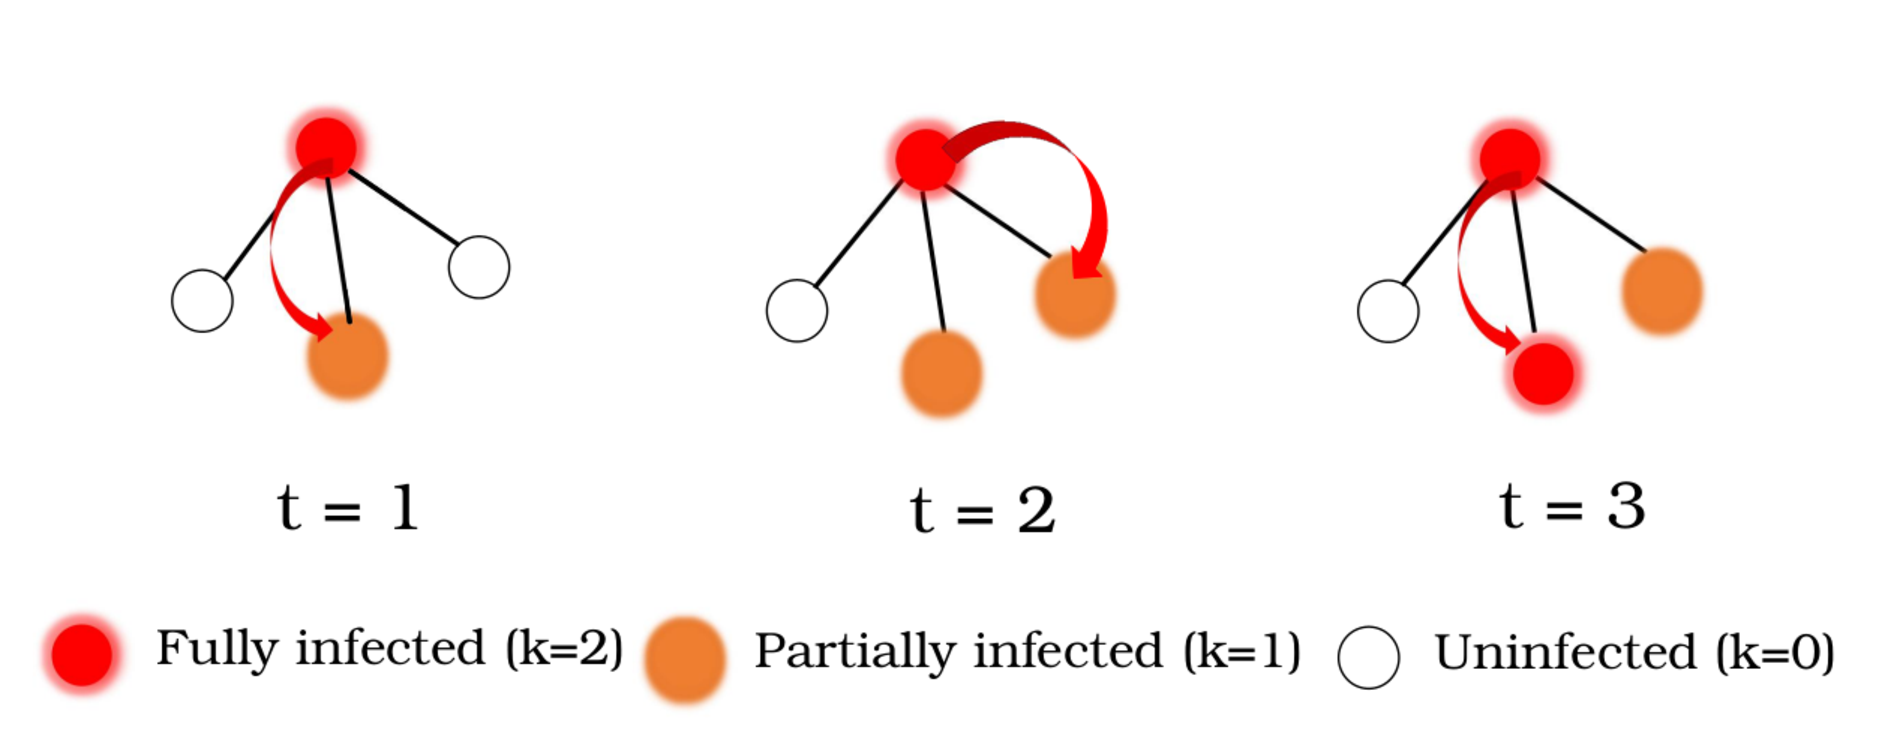
\includegraphics[scale=0.37]{./texfiles/Chapter_3/epl/figs1/dynamics.pdf}
  %\includegraphics*[scale=0.28]{figs1/plot_var_k.eps}
 %\includegraphics*[scale=0.15]{figs/T1_vs_exp_T1_d_reg.eps}
 
%\hspace{5mm}(a)\hspace{75mm}(b) 
%\vspace{-2mm}
 \caption{\label{fig_dynamics}Proposed diffusion model for $k=2$.}
 %\vspace{-.5cm}
\end{figure}
 
 
 \begin{figure}[htpb]
 %\vspace{-.5cm}
  \centering
  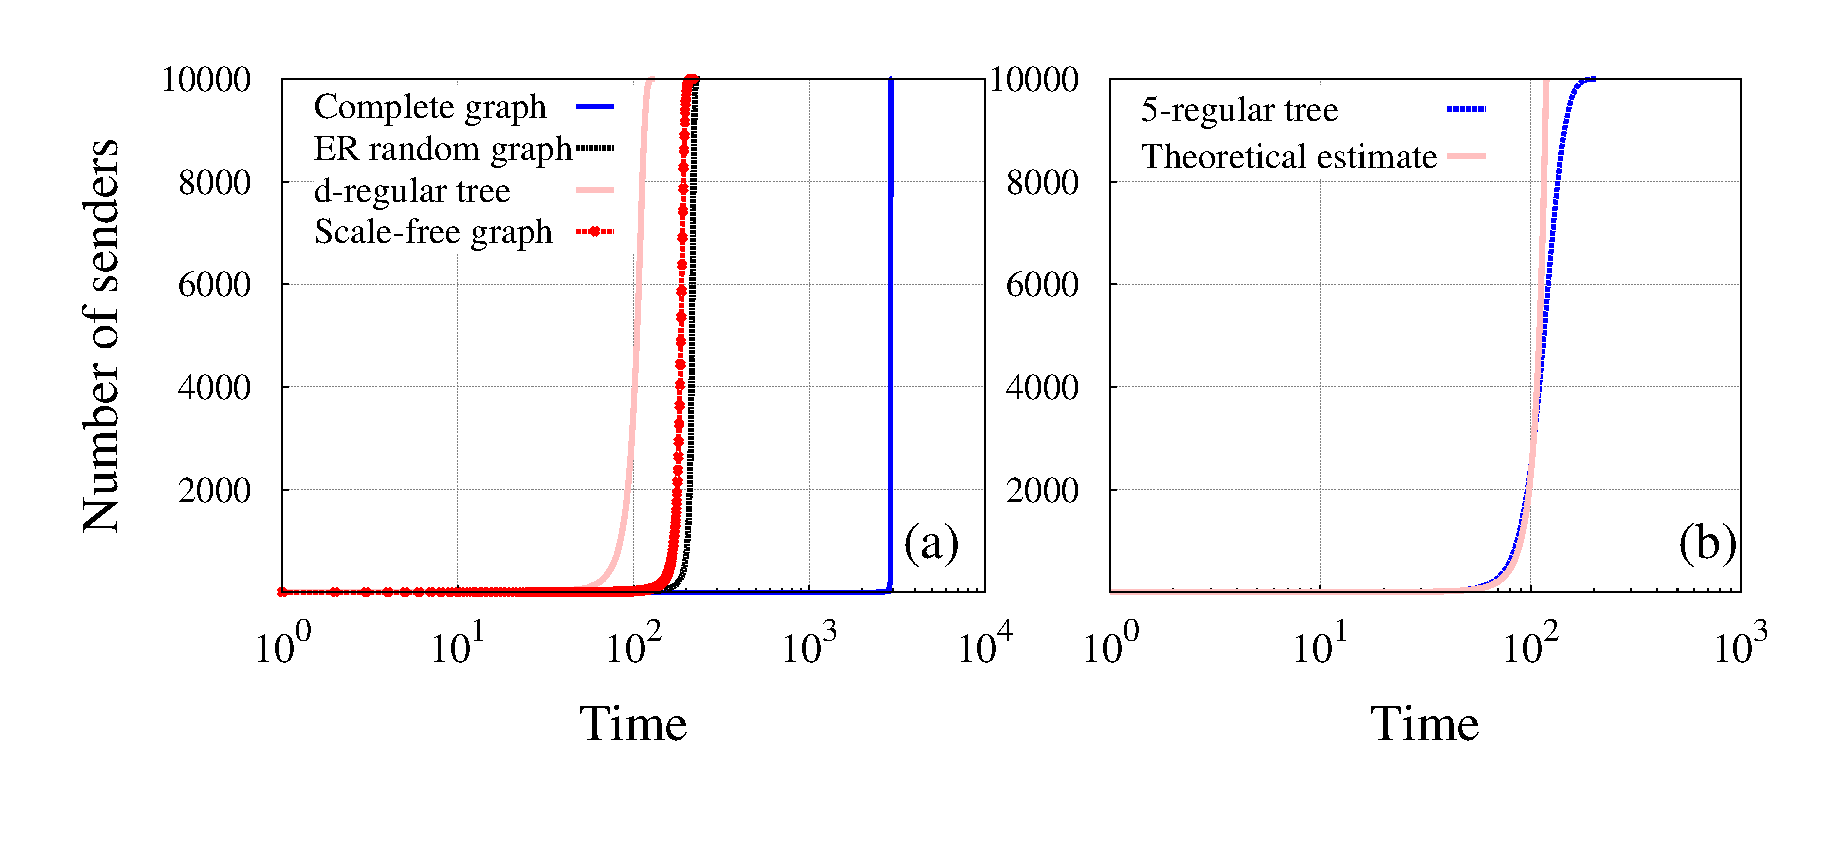
\includegraphics[scale=0.38]{./texfiles/Chapter_3/epl/figs1/plot_all.eps}
  %\includegraphics*[scale=0.28]{figs1/plot_var_k.eps}
 %\includegraphics*[scale=0.15]{figs/T1_vs_exp_T1_d_reg.eps}
 
%\hspace{5mm}(a)\hspace{75mm}(b) 
%\vspace{-4mm}
 \caption{\label{fig1} (a) The number of senders versus time steps for different network topologies (For ER random graph $p$ is $0.005$, for $d$-regular graph $d=5$ and for BA scale-free graph $m$ i.e., number of edges to attach from a new node to existing nodes is $5$) and 
 (b) The theoretical estimate and the simulated result for $d-$regular trees. The theoretical eastimate is obtained from equation 17.}
 %\vspace{-.5cm}
\end{figure}
 
% \todo{In figure~\ref{fig1} caption, add the vlaue of $p$ for ER graph and $\lambda$ for the scale-free graphs.}
 
Formally, we consider a network topology $G$ = $(V,E)$ where $V$ represents the set of
nodes in the network and $E$ denotes the set of edges between any pair of nodes in $%
V $. We initially start with a single infected node in the system. We
further assume that for a susceptible node to get infected,  $k$ encounters
with infected nodes are required. To put it in a simple way we consider that
a message $M$ needs to be spread over a network and message $M$ consists of $%
k$  identical tokens. At each communication instance one token gets transmitted from an
infected node to the susceptible node. Therefore, number of tokens ($k$) in a
message corresponds to the number of contacts required for a susceptible
node to get infected. Note that for the rest of the paper we will present
our diffusion model in terms of messages and tokens. 
%Since the infected nodes essentially pass on the tokens we term them as senders while the susceptible ones are the non-senders.  

We assume that at time $0$, there is only one sender (infected) node present in the
system and it acts as the {\em initiator} of the diffusion process. At each
discrete time step a sender node randomly selects one of
its neighbors and  there is a transfer of a token from the sender to the non-sender. A non-sender node becomes a sender only after it receives exactly $k$
tokens (refer to figure \ref{fig_dynamics}). 
The analytical
estimation of the diffusion time based on the underlying topology requires a
case-by-case examination.
We formulate both analytical and empirical results for two extreme variants (in terms of edge density) of networks (a) complete graphs (dense) and (b) infinite regular trees (sparse)
while for others we provide empirical
results with intuitive justifications.
%\todo{Can we have a small picture demonstrating the dynamics since this is a very novel concept? We can take a small network, $k=3$ and illustrate the spread in three time points -- $t=0$ where only one node is black (the initiator), some intermediate $t=t^{'}$ where we show the $k$ values for different nodes (none of which is yet $=3$) and then $t=t^{''}$ where the first sender is formed (one node has $k=3$). We have enough white spaces between figures which can be reduced to fit in this picture.}
\if{0}
%Note that this results in creation of a subgraph at each time step roughly resembling a temporal network. 
% Assuming such a diffusion model we study in detail the diffusion time (i.e.,
% the time from the start till the time when all the nodes in the network
% receive the information and the algorithm terminates) given an underlying
% network topology.
\fi
% \begin{figure}[htpb]
%   \centering
%   \includegraphics[scale=0.28]{figs1/plot_var_k.eps}
%   %\includegraphics*[scale=0.28]{figs1/plot_var_k.eps}
%  %\includegraphics*[scale=0.15]{figs/T1_vs_exp_T1_d_reg.eps}
%  
% %\hspace{5mm}(a)\hspace{75mm}(b) 
%  \caption{\label{fig_k} Number of nodes at each stage of infection versus time for complete graph \todo{write more detailed description}}
% \end{figure}


\if{0} 
% \subsection{Agent configuration and network setup}
% 
% We consider a network topology $G = < V,E >$ where each node in $V$ represents an agent of the network and any link in $E$ represents a contact 
% opportunity between a pair of nodes (agents) in the whole time span through which the network is active. So for any node (agent) $n_{i}$ in this network, its one hop 
% neighbors are the nodes (agents) which are within the connection proximity of $n_{i}$ and at each time step $n_{i}$ at random can connect to any one of them. 
% 
% 
% \subsection{Information configuration}
% 
% As we stated earlier, we consider that the information diffusion occurs in parts. 
% We consider that thdie whole information $\mathcal{M}$ is divided into a set of $m$ tokens, i.e., $|\mathcal{M}| = m$ and in 
% a contact opportunity a single token gets transmitted.
%  We can also extend it to knowledge diffusion or special cases of disease spreading where a susceptible node gets infected 
%  only after it meets infected individuals for specified number of times. In these cases the total number of tokens 
%  would refer to the number of times ($m$) a susceptible (novice) individual communicates with an infected (knowledgeable) individual 
%  before it itself gets infected (knowledgeable). It can further be interpreted as the number of times a node should be reminded of an 
%  information before it remembers and participates in the diffusion process. Note that throughout our analysis we will stick to the 
%  notion of information and tokens for simplicity. 
% 
% 
% \subsection{Information diffusion technique}
% 
% In this framework, transfer of a message during a contact refers to the transfer of one single token of the information. 
% Transfer of a token from $u_i$ to $v_j$ during a contact can take place only 
% when $u_i$ qualifies as a {\em sender} by having all the tokens of the information.
% We mainly consider the $push$ technique of information diffusion which is described below. 
% 
% 
%  \noindent \emph{Push technique:} 
%   \begin{itemize}
%  % \vspace{-3mm}
%    \item \emph{Step 1:} At any time step, $u_i$ (already a sender) establishes a communication link with $v_j$, 
%    from its neighborhood and finds an exclusive set of tokens that $u_i$ has but $v_j$ does not have in its buffer. 
%    \item \emph{Step 2:} If $u_i$ can find such a (non-empty) set, then it transfers only one token from this set to $v_j$. 
%   \end{itemize}
% 
% Next we describe the information diffusion technique which we call $Blind Push$ (B-P) in detail.
% An initiator node is the one which has the full information in the beginning. At each time step all the nodes 
% in the system having the full information communicate with a node in their proximity and try to $push$. 
% %If it is successful then a unit bandwidth is consumed otherwise it is counted as wastage. 
% At the end of each time step all the nodes which have received all the tokens qualify as sender in the next time step. The algorithm terminates 
% when all the nodes in the system have the full information.
% We consider two types of epidemic processes - a) Susceptible-Infected (SI) and b) Susceptible-Infected-Recovered (SIR). 
% Susceptible nodes are the ones having a subset ($S$) of all the tokens ($0\leq |S| < m$, partial information) and the infected nodes are the one with 
% all the tokens (full information). The recovered nodes are the ones, which after having received the full information and spreading it for some time 
% have moved out of the system and is no longer part of the network.
% The information diffusion technique is similar for both the process. 

% \begin{algorithm}
% \caption{Blind Push (B-P)}\label{bp}
% \begin{algorithmic}[1]
% %\Procedure{MyProcedure}{}
% \STATE $select \, initiator$
% \STATE $make \, it \, sender$
% %\BState \emph{top}:
% %\If {$i > \textit{stringlen}$} \Return false
% %\EndIf
% %\State $j \gets \textit{patlen}$
%  \WHILE {$( not \, all \, nodes \, in \, the \, network \, have \, the \, message )$}
%  \FOR {$(each \, node \, which \, is \, already \, a \, sender)$}
% \STATE $select \, a \, node \, from \, its \, proximity;$
% \STATE $perform \, Push$;
% \IF {$(Push \, unsuccessful)$}
% \STATE $wastage;$
% \ELSE 
% \STATE $unit \, bandwidth \, consumed;$
% %\State $i \gets i-1$.
% %\State \textbf{goto} \emph{loop}.
% %\State \textbf{close};
% \ENDIF
% \ENDFOR
% \STATE $modify \, the \, list \, of \, senders;$
% \STATE $increment \, time;$
% \ENDWHILE
% %\EndProcedure
% \end{algorithmic}
% \end{algorithm}

% \subsection{Metrics of interest}
% %\vspace{-2mm}
% We are interested in evaluating the spreading model in terms of the following metrics-
% \begin{itemize}
% %\vspace{-4mm}
%  \item \textbf{Diffusion time $T^*$} - this is the time from the point when the message source starts the diffusion process to the point when all the agents in the network have received the the total information. 
%  $E(T^*)$ denotes the expected diffusion time. In addition, we are also interested in the time $T_i$ which is the minimum time at which there are $i$ senders (except the source) in the network, and especially in $T_1$ since, as we shall see, that this is the prime determinant of the entire broadcast time. 
% %\todo{why are these lines needed - Finally, note that $T^*$ may not correspond to $T_{n-1}$, i.e., the time when there are $n-1$ senders (except the source) in the network because all $n-1$ agents need not become senders to spread the message.}  
%  \item \textbf{Diffusion threshold} - 
% \end{itemize}
% \subsection{Dynamic topology}
% %\vspace{-2mm}
% We performed our experiments on synthetic topologies like complete graph, regular tree, regular graph and random graph. 
% A topology specifies the potential neighborhood of a node 
% - a node at each time step connects randomly to one of these nodes. A complete graph 
% topology would indicate that the 
% node can connect to any other node in the network while for other sparser topology it would 
% connect only to a subset of them.

\medskip
\fi



\noindent
\section{On Complete graph}
\label{res_complete}
\noindent For {\bf complete graph} we assume the
number of nodes in the system to be $n$. 
%The time elapsed before the first sender (apart from the initiator) is created is represented by $t_1$ and the total diffusion time is denoted by $T^*$. We denote the expected values of these quantities by $% \mathbb{E}(t_1)$ and $\mathbb{E}(T^*)$ respectively. 
To determine how the number of
senders in the system changes with time, we plot the number of senders
against time for complete graph in Fig.~\ref{fig1}. 
%We further show in ~\ref{fig_k} how the diffusion progresses by plotting the number of nodes at each stage of infection at every time step for complete graph topology which roughly resembles epidemic process on a heterogenous population.  %Note
%that we assume the $d$-regular tree to be truncated with all the nodes except the leaf
%nodes have degree $d$.
We observe that the diffusion is initially slow which is then followed by a ramp-up after which the diffusion rate becomes almost exponentially fast.
To better analyze the process we divide the process into two phases i) the initial phase and ii) the residual phase. 


\noindent{\bf Initial phase:}  In the spreading process we define the initial phase to be the time between the
initiation and the point at which the first sender is created. We
define this as $t_1$; we will show later that $\hat E(t_1)$ (expected value of $t_1$) is
indeed an indicator for $\hat E(T^*)$ ($T^*$ - 
total diffusion time) in case of a complete graph.

Note that analytically deriving  $\hat E(t_1)$ assuming a  discrete 
(i.e., for a node the delay between two successive contacts is $1$ unit) diffusion model becomes severely complex and hence we adopt a continuous 
variant of the model. In fact, the calculation of the $\Pr \{ t_{1}=t\}$ can be treated as an expected time of filling the first urn with $k$
balls in the experiment where we have initially $d$ empty urns (degree of the node, for complete graph $d \sim n$) and at each
single time step we add a single ball to one urn chosen randomly. 
 For any $k$%
-parts message, by~\cite{kaplan1977generalization} we describe our problem
as a unit-time Poisson process. Note that for a poisson process the inter-arrival time follows exponential distribution ($\lambda$) and expected number of arrivals in time $t$ is $\lambda t$.  
 Let 
$X_{j}(t)$ be a random value describing the number of balls in $j^\textrm{th}$ urn up
to time $t$. More precisely $X_{j}(t)=\sum_{i=1}^{N}1$ where $N$ is a random variable 
with Poisson distribution $\mathcal{P}(\frac{t}{d})$. Essentially $N$ represents number of draws
of the $j^\textrm{th}$ urn up to time $t$ if $d$ urns exist in the system.
Hence $\{X_{j}(t)\}$s are i.i.ds and $X_{j}(t)\sim\mathcal{P}(\frac{t}{d}%
) $.  
{We formulate the analytical result for complete graph topology through the following theorems 1-5. The various notations are further 
summarized in table \ref{tab:1}}



\begin{theorem}
%\vspace{-.2cm}
For a message with $k$ tokens, the expected value of $t_1$, 
$\hat E(t_{1})=\int_{0}^{\infty}(1-P(t_{1}\leq
t))dt = \int_{0}^{\infty}Q(k,\frac{t}
{d})^{d}dt$
where $Q(k,u)$ is a regularized incomplete gamma function and $d$ is the degree. 
% Furthermore for fixed $i\geq 2$ the random variable $t_{i}d^{-\frac{k-1}{k}}$ converges to a limiting random variable $\tau _{i}$ and the following recursion holds for the expectations: $\frac{\mathbb{E}\left( \tau _{i}\right) }{\mathbb{E}\left( \tau _{i-1}\right) }%=1-\frac{2k-1}{ik} .$
\label{theorem-0}
\end{theorem}

\begin{proof}
 \begin{equation}
\begin{aligned} 
\hat E(t_{1})=&\int_{0}^{\infty}(1-P(t_{1}\leq
t)dt=\int_{0}^{\infty}(1-(1-P(t_{1}
>t))dt\\=&\int_{0}^{\infty}P(X_{j}(t)<k)^{d}dt=\int_{0}^{\infty}Q(k,\frac{t}
{d})^{d}dt\label{eqint} 
\end{aligned}
\end{equation}

where $Q(k,u)$ is a regularized incomplete gamma function i.e. 
\begin{equation}
Q(k,u)=\frac{\Gamma(k,u)}{\Gamma(k)}=e^{-u}\sum_{l=0}^{k-1}\frac{u^{l}}{l!}
\end{equation}
is valid for any natural $k$ and non-negative $u$.

\end{proof}

%\vspace{-.2cm}
Note that $t_{1}$ for a Poisson process, is a continuous random variable. 

\noindent{\bf Residual phase:} We next proceed to establish the relation between $\hat E(t_1)$ and $\hat E(T^{*})$. Apart from assuming the continuous model, 
we compute scaled $t_1$ and $T^{*}$ (by $d^{\frac{k-1}{k}}$, 
(this specific scaling function was initially calculated for $k=2$ and then generalized for higher values)) instead of their explicit values to further aid our analysis. 
To summarize, we start by computing  
expected values of scaled $t_1$ and $T^{*}$ considering a continuous (Poisson) model with $d\rightarrow \infty$ and show that the results hold for finite $d$. Finally we show that the results for the continuous model extend to the discrete model.
We begin by showing that $t_1$ (time to create the first sender apart from the initiator) is an indicator for the diffusion delay $T^*$ through the following two theorems. 
%The detailed proof of both the theorems are available in the supplementary.


\begin{table}
\centering
\caption{Summary of the notations used.}
\label{tab:1}
\scalebox{0.65}{
\begin{tabular}{|l|l|}
\hline
{\bf Symbol}             & {\bf Definition}                                                                     \\ \hline\hline
$t_1$              & Time between initiation and creation of first sender                           \\ \hline
$T^{\ast}$         & Total diffusion time                                                           \\ \hline
$\hat E(t_1)$      & Expected $t_1$ (obtained analytically)                                         \\ \hline
$\hat E(T^{\ast})$ & Expected $T^{\ast}$(obtained analytically)                                     \\ \hline
$Av(t_1)$          & Expected $t_1$ (obtained empirically)                                          \\ \hline
$Av(T^{\ast})$     & Expected $T^{\ast}$ (obtained empirically)                                     \\ \hline
$s_1$              & Limiting random variable of $t_{1}d^{- \frac{k-1}{k}}$as $d\rightarrow \infty$ \\ \hline
$\tau_i$           & Scaled time span between creation of $(i-1)^{th}$ sender and $i^{th}$ sender   \\ \hline
$s^{\ast}$         & Limiting random variable for $T^{\ast}d^{-\frac{k-1}{k}}$                      \\ \hline
\end{tabular}}
\end{table}

\begin{theorem}
%\vspace{-.2cm}
For a message with $k$ tokens the random variable $t_{1}d^{-\frac{k-1}{k}}$
converges as $d\rightarrow \infty $ to a limiting random variable $s_{1}$
with density $\frac{x^{k-1}}{(k-1)!}e^{-\frac{x^{k}}{k!}}$ 
and expectation $%
\hat E \left( s_{1}\right) =(k!)^{\frac{1}{k}}\Gamma\left(1+\frac{1}{k%
}\right).$ 
% Furthermore for fixed $i\geq 2$ the random variable $t_{i}d^{-\frac{k-1}{k}}$ converges to a limiting random variable $\tau _{i}$ and the following recursion holds for the expectations: $\frac{\mathbb{E}\left( \tau _{i}\right) }{\mathbb{E}\left( \tau _{i-1}\right) }%=1-\frac{2k-1}{ik} .$
\label{theorem-1}
\end{theorem}
%\vspace{-.2cm}

\begin{proof}
 The proof is based on Poisson clock approximation approach
introduced {previously.} 
% which means that variables are
% independent and for a price of acceptable level of error of the order $%
% o_d(1) $. 
We start from the calculation of the CDF for the random variable $%
t_1 d^{-\frac{k-1}{k}}$:


\begin{equation}
\begin{aligned} &F_{t_1 d^{-\frac{k-1}{k}}}(x)=P(t_1 d^{-\frac{k-1}{k}}\leq
x)\\
%=1-P(t_1>xd^{\frac{k-1}{k}})\\
%&=1-P(X_j(xd^{\frac{k-1}{k}})<k)^d
&=1-Q(k,\frac{xd^{\frac{k-1}{k}}}{d})^d%
\\
&=1-\left(\sum_{i=0}^{k-1}e^{-xd^{-\frac{1}{k}}}(xd^{-%
\frac{1}{k}})^i/i!\right)^d\\ \label{eq-prof-1}
%&=1-\left(1-e^{-xd^{-\frac{1}{k}}}(xd^{-%
%\frac{1}{k}})^k/k!(1+o(1))\right)^d 
 \end{aligned}
\end{equation}

where in the last line we used the common simple approximation of Poisson
cumulative distribution in long tail.

Since we are interested in limits as $d\rightarrow \infty$, for $%
exp(-xd^{-\frac{1}{k}})\rightarrow 1$ and we can compute limits of $F_{t_1
d^{-\frac{k-1}{k}}}$ 
as follows: 
\begin{equation}
\begin{aligned} F_{s_1}(x)&=\lim_{d\rightarrow\infty}F_{t_1
d^{-\frac{k-1}{k}}}(x)\\&=\lim_{d\rightarrow\infty}1-\left(\sum_{i=0}^{k-1}e^{-xd^{-\frac{1}{k}}}(xd^{-%
\frac{1}{k}})^i/i!\right)^d \\&=
1-e^{(-x^k/k!)} \label{eq-prof-cdf1} \end{aligned}
\end{equation}

Now, the density function of $\tau_1$ can be calculated as - 

\begin{equation}
f_{s_1}(x)=\frac{dF_{s_1}}{dx}(x)=\frac{x^{k-1}}{(k-1)!}exp%
\left(-\frac{x^{k}}{k!}\right)
\end{equation}
Further the expectation of $s_{1}$ is - 
 \begin{equation}
\begin{aligned}
\hat E(s_1)&=\int_{0}^{\infty}xf_{s_1}(x)dx=\int_{0}^{\infty}%
\left(uk!\right)^{\frac{1}{k}}e^{-u}du\\&=\left(k!\right)^{\frac{1}{k}}%
\int_{0}^{\infty}u^{\frac{1}{k}}e^{-u}du=\left(k!\right)^{\frac{1}{k}}\Gamma%
\left(1+\frac{1}{k}\right) \label{e-tau-1} 
\end{aligned}
\end{equation}
\end{proof}



We next compute the expectation of the (scaled) time $%
T^{\ast }$ till all nodes become senders.  
We consider $T_{i}=t_{i}d^{-\frac{k-1}{k}}$. We further assume $\tau _{i}$ as the
scaled time span between the creation of $(i-1)^\textrm{th}$ new sender and that of $i^\textrm{th}$ new
sender. Correspondingly $\tau _{i}^{\ast }$ represents the scaled time for
the original process where every node with at least $k$ tokens acts as a
sender node.  
We have $\hat E\left( \tau _{i}^{\ast }\right) =%
\frac{1}{i}\hat E\left( \tau _{i}\right) =\frac{1}{i}\left( \hat E%
\left( T_{i}\right) -\hat E\left( T_{i-1}\right) \right)$.  
Note that $\tau _{1}$ is equal to $T_{1}$ as $T_{0}$ is 0 and hence $\hat E(s_1)$ equals $\hat E(\tau _1)$.
%\vspace{-.2cm}
\begin{theorem}
%\vspace{-.2cm}
\label{theorem-2} $T^{\ast }d^{-\frac{k-1}{k}}$ converges to a limiting
random variable $s^{\ast }$ with 
%\vspace{-.2cm}
\begin{equation*}
\vspace{-.3cm}
\hat E \left( s^{\ast }\right) =\sum\limits_{i=1}^{\infty }\hat E%
\left( \tau _{i}^{\ast}\right) = \hat E(\tau_1)\frac{k}{k-1}
\end{equation*}
\end{theorem}

\begin{proof}
$G_{i}^{\left( d\right) }\left( z\right)
=1-F_{i}^{\left( d\right) }\left( z\right) =\Pr \left\{ t_{i}>zd^{\frac{k-1}{%
k}}\right\} =\Pr \left\{ T_{i}>z\right\} $(complementary cdf of $T_i$). Since $\frac{zd^{\frac{k-1}{k}}}{%
d}=zd^{-\frac{1}{k}}$ we have 
\begin{equation}
\begin{aligned} G_{i}^{\left( d\right) }\left( z\right)
=&\sum_{j=0}^{i-1}\binom{d}{j}\left( \sum_{l=0}^{k-1}\frac{1}{l!}\left(
zd^{-\frac{1}{k}}\right) ^{l}e^{-zd^{-\frac{1}{k}}} \right)
^{d-j}\\&\left( 1-\sum_{l=0}^{k-1}\frac{1}{l!}\left(
zd^{-\frac{1}{k}}\right) ^{l}e^{-zd^{-\frac{1}{k}}} \right)
^{j} \\
%=&\sum_{j=0}^{i-1}\binom{d}{j}\left( 1-\left( 1+o_{d}\left( 1\right)
%\right) \frac{z^{k}d^{-1}}{k!}e^{-zd^{\frac{-1}{k}}}\right) ^{d-j}\\&\left(
%\left( 1+o_{d}\left( 1\right) \right)
%\frac{z^{k}d^{-1}}{k!}e^{-zd^{\frac{-1}{k}}}\right) ^{j} \\
%=&\sum_{j=0}^{i-1}\frac{d^{j}}{j!}\left( \frac{z^{k}}{k!}\right)
%^{j}\frac{1}{d^{j}}e^{-\frac{z^{k}}{k!}}\left( 1+o_{d}\left( 1\right)
%\right) \\
=&\sum_{j=0}^{i-1}\frac{1}{j!}\left( \frac{z^{k}}{k!}\right)
^{j}e^{-\frac{z^{k}}{k!}}\left( 1+o_{d}\left( 1\right) \right) 
\end{aligned}
\end{equation}
taking limits $d\rightarrow \infty $ and using the abbreviation $a=\frac{%
z^{k}}{k!}$ we obtain for $G_{i}\left( z\right) =\lim_{d\rightarrow \infty
}G_{i}^{\left( d\right) }$ and
%=1-F_{i}\left( z\right) $ the expression%
%\todo{I dont see any usage of $F_i$ so why mentioning it in a equation (9). - remove eq. 9}
\begin{eqnarray}
G_{i}\left( z\right) &=&\sum_{j=0}^{i-1}\frac{a^{j}}{j!}e^{-a} 
\end{eqnarray}
%F_{i}\left( z\right) &=&1-\sum_{j=0}^{i-1}\frac{a^{j}}{j!}e^{-a}.
%
Subsequently,  we get for $\hat E \left( \tau _{i}\right) =\int \left(
G_{i}\left( z\right) -G_{i-1}\left( z\right) \right) dz:$%
\begin{eqnarray}
\hat E \left( \tau _{i}\right) &=&\int_{0}^{\infty }\frac{1}{\left(
i-1\right) !}\left( \frac{z^{k}}{k!}\right) ^{i-1}e^{-\frac{z^{k}}{k!}}dz ,
\\
\hat E \left( \tau _{i}^{\ast }\right) &=&\int_{0}^{\infty }\frac{1}{i}%
\frac{1}{\left( i-1\right) !}\left( \frac{z^{k}}{k!}\right) ^{i-1}e^{-\frac{%
z^{k}}{k!}}dz .
\end{eqnarray}%
For computing $\mathop{\displaystyle \sum }\limits_{i=1}^{N}\hat E\left(
\tau _{i}^{\ast }\right) $ we can exchange integration and summation. Hence
we first estimate 
\begin{equation}
\begin{aligned} \lim_{N\rightarrow \infty }\mathop{\displaystyle \sum
}\limits_{i=1}^{N}\frac{1}{ i !}a^{\left( i-1\right) }e^{-a}
&=&\frac{1}{a}\left(
1-e^{-a}\right)
%&\lim_{N\rightarrow \infty }\frac{1}{a}\mathop{\displaystyle \sum
%}\limits_{i=0}^{N}\frac{1}{(i+1)!}a^{i+1}e^{-a} \\ 
%&=&\frac{1}{a}\left(
%1-e^{-a}\right). 
\end{aligned}
\end{equation}

Transforming variables in the integral as $y=\frac{z^{k}}{k!}$ we
finally get 
\begin{equation}
\hat E \left( s^{\ast }\right) =\frac{\left( k!\right) ^{\frac{1}{k}}}{k-1%
}\Gamma \left( \frac{1}{k}\right)= \hat E(\tau_1)\frac{k}{k-1}
\end{equation}

\end{proof}

We observe from the above result that the expectation of scaled $T^{*}$ converges to a value which depends only on $k$ which is constant for a given setting. 
Hence we conclude that the expectation of {\bf $T^{*}$ is proportional to $d^{\frac{k-1}{k}}$} and similarly for $t_1$.

The above results are based on the assumption that $i$ is fixed as  
%as I understand the number of sender would also increase exponentially - then does the limit hold}) is fixed and $%
$d\rightarrow \infty .$  
We now proceed to show that the computations hold for finite $d$ for $i$ varying with $d$.
Note that the above formulas hold true for $i\leq f\left( d\right) $ as
long as $f\left( d\right) =o\left( d^{\frac{1}{k}}\right) .$ 


\begin{theorem}
%\vspace{-.2cm}
\label{theorem-3}
Considering that the range of $i$ (number of senders) varies with $d$ (degree) if $f\left( d\right) =d^{\frac{1}{k}-\epsilon }$
for some $\epsilon >0$, %
$\sum_{i>f\left( d\right) }^{d}\tau _{i}^{\ast }\left( d\right) =o_{d}\left(
\sum_{i\geq 1}^{f\left( d\right) }\tau _{i}^{\ast }\left( d\right) \right) $
\end{theorem}
%\vspace{-.2cm}

\begin{proof}
We compute first $\mathbb{E}\left( \tau _{i}\right)
=\int_{0}^{\infty }\frac{1}{\left( i-1\right) !}\left( \frac{z^{k}}{k!}%
\right) ^{i-1}e^{-\frac{z^{k}}{k!}}dz$ using again the transformation of
variables $y=\frac{z^{k}}{k!}$

\begin{eqnarray}
\hat E \left( \tau _{i}\right) &=&\frac{1}{\left( i-1\right) !}\frac{\left( k!\right) ^{1/k}}{%
k}\int_{0}^{\infty }y^{i-2+\frac{1}{k}}e^{-y}dy \\
&=&\frac{1}{\left( i-1\right) !}\frac{\left( k!\right) ^{1/k}}{k}\Gamma
\left( i-1+1/k\right)
\end{eqnarray}

%.

%\todo{Lets discuss this part}

%For large $i$ we have by Stirlings formula $\Gamma \left( i-1+1/k\right)
%\simeq \sqrt{2\pi }\frac{\left( i-2+1/k\right) ^{i-3/2+1/k}}{e^{i-2+1/k}}$
%and
Using Stirlings approximation we obtain - \\
%$\left( i-1\right) !\simeq \sqrt{2\pi \left( i-1\right) }\left( \frac{i-1%
%}{e}\right) ^{i-1}$ hence 
\begin{equation}
\frac{\Gamma \left( i-1+1/k\right) }{\left( i-1\right) !}\simeq e^{-2+\frac{2%
}{k}}\frac{1}{\left( i-1\right) ^{1-1/k}}
\end{equation}
The further argumentation is independent of the involved constant
coefficients since we only need leading orders.

We have -  
\begin{equation}
\begin{aligned} T_{L}&=\sum_{1}^{L}\hat E \left( \tau _{i}\right)
=O\left( 1\right) \cdot \sum_{1}^{L}\frac{\Gamma \left( i-1+1/k\right)
}{\left( i-1\right) !}\\&=O\left( 1\right)
\int_{1}^{L}\frac{1}{x^{1-1/k}}dx= O\left( 1\right) L^{1/k}. \end{aligned}
\end{equation}

Note once more that all the computations up to now are in scaled time units.
Hence in real time we have $t_{L}\sim $ $L^{1/k}d^{1-\frac{1}{k}}.$ Setting $%
L\sim d^{\frac{1}{k}-\epsilon }$ we get $t_{L}=d^{1-\frac{1}{k}+1/k^{2}-%
\frac{\epsilon }{k}}.$ Taking $t_{L}$ as unit and taking into account that
the total time $t^{\ast }$ (in the scaled process) is according to the
results in Erd\"{o}s and Kaplan \cite{kaplan1977generalization} $t^{\ast
}=\left( 1+o\left( 1\right) \right) d\log d$ we have $t^{\ast }=$ $O\left(
1\right) \cdot t_{L}\cdot d^{\frac{1}{k}-1/k^{2}+\frac{\epsilon }{k}}\log d.$
But since the acceleration at this point is $d^{1/k-\epsilon }$ we have for
the remaining time (that is the time after the $d^{\frac{1}{k}-\epsilon }$%
-th event) in the accelerated process a contribution of at most $\tilde{t}%
_{L}d^{-1/k^{2}+\frac{\epsilon }{k}+\epsilon }\cdot \log d=\tilde{t}%
_{L}\cdot o_{d}\left( 1\right) $ since $\epsilon $ can be chosen arbitrary
small - here $\tilde{t}_{L}$ denotes the time till the $L^\textrm{th}$ event in the
accelerated process. This shows that $\sum_{i>f\left( d\right) }^{d}\tau
_{i}^{\ast }\left( d\right) =o_{d}\left( \sum_{i\geq 1}^{f\left( d\right)
}\tau _{i}^{\ast }\left( d\right) \right) .$

\end{proof}

{The above results show that previous computations (considering $d\rightarrow \infty$) give correct limiting values. 
This indicates that our analysis is able to correctly estimate the diffusion time for a complete graph of finite size.}


It now remains to show that the asymptotic estimations for the model with
Poisson clock carry over to the discrete time model (which we use for our simulations) defined at the
beginning. Note that the discrete time model is actually the Poisson
model when looked at in event time steps, where events here are the
times when a token is sent. 
%Consider first the time $t_{i}$ that is the
%real time between the creation of $(i-1)$$^\textrm{th}$ and $i$$^\textrm{th}$ sender in the Poisson model. 

\begin{theorem}
%\vspace{-.2cm}
 If $t_{i}$ is the time between the creation of the $(i-1)^\textrm{th}$ and $i^\textrm{th}$ sender and 
 $\hat{t}_{i}$ is the corresponding time in the discrete model, then $\hat E \left( \hat{t}_{i}\right) =\hat E \left( t_{i}\right)
\left( 1+o_{d}\left( 1\right) \right) $ 
\end{theorem}
%\vspace{-.2cm}
%\todo{Is the proof starting here?}
\begin{proof}
Since we have $i$ independent senders all acting with Poisson clocks of
intensity $1$ we have the time between two tokens sent - denoted in the
following by a random variable $x$ - to be an exponential distribution $%
Exp\left( i\right).$ We index the events by $l$ and observe that $t_{i}=%
\sum\limits_{l=1}^{K_{i}}x_{l}$ where $K_{i}$ is the
random stop time when the $i^\textrm{th}$ sender is created. In the discrete model $i$
messages are sent simultaneously 
hence $i$ successive events in the Poisson
model correspond to one time step in the discrete model. Hence $\hat{t}%
_{i}=\left\lfloor \frac{1}{i}\cdot K_{i}\right\rfloor =\frac{1}{i}\cdot
K_{i}\cdot \left( 1+o_{d}\left( 1\right) \right) $ . Since the $\left\{
x_{l}\right\} $s are i.i.ds we can apply Wald's theorem \cite{wald} and get 
\begin{center}
$\hat{E}\left( t_{i}\right) =\hat{E}\left( K_{i}\right) \hat{E}%
\left( x\right) =\frac{1}{i}\hat{E}\left( K_{i}\right)$ 
\end{center}%
hence $\hat{E}\left( \hat{t}_{i}\right) =\hat{E}\left( t_{i}\right)
\left( 1+o_{d}\left( 1\right) \right) $ and the analytical results for the poisson model hold for the discrete case as well.
\end{proof}

We further simulated our diffusion model on complete graphs to verify our analytical results. 
For this
purpose, we plot in figure \ref{segSizeVsDelay_nrTrans_varyN_Mall_push_pull}
the values of {average diffusion time ($Av(T^{\ast })$)} and {average time to create the first sender ($Av(t_{1})$)} respectively as we vary the size of the network. We further 
report the values of $Av(T^{\ast })$ and $Av(t_{1})$ for different values of $k$
with network size fixed at $1000$. 
Note that
the two quantities $Av(T^{\ast })$ and $Av(t_{1})$ (the results were averaged over $1000$ simulations) exhibit a
very similar profile irrespective of the chosen value of $k$. 
In the same
figure we also plot the function 
 $d^{\frac{k-1}{k}}$ (represented by $\hat E(t_1)$) { obtained from theorem \ref{theorem-1}}, suitably scaled by a
constant to show how the theoretical results closely follow  the
numerical simulations.

 \begin{figure}[htbp] 
 %\vspace{-.3cm}
 \centering
 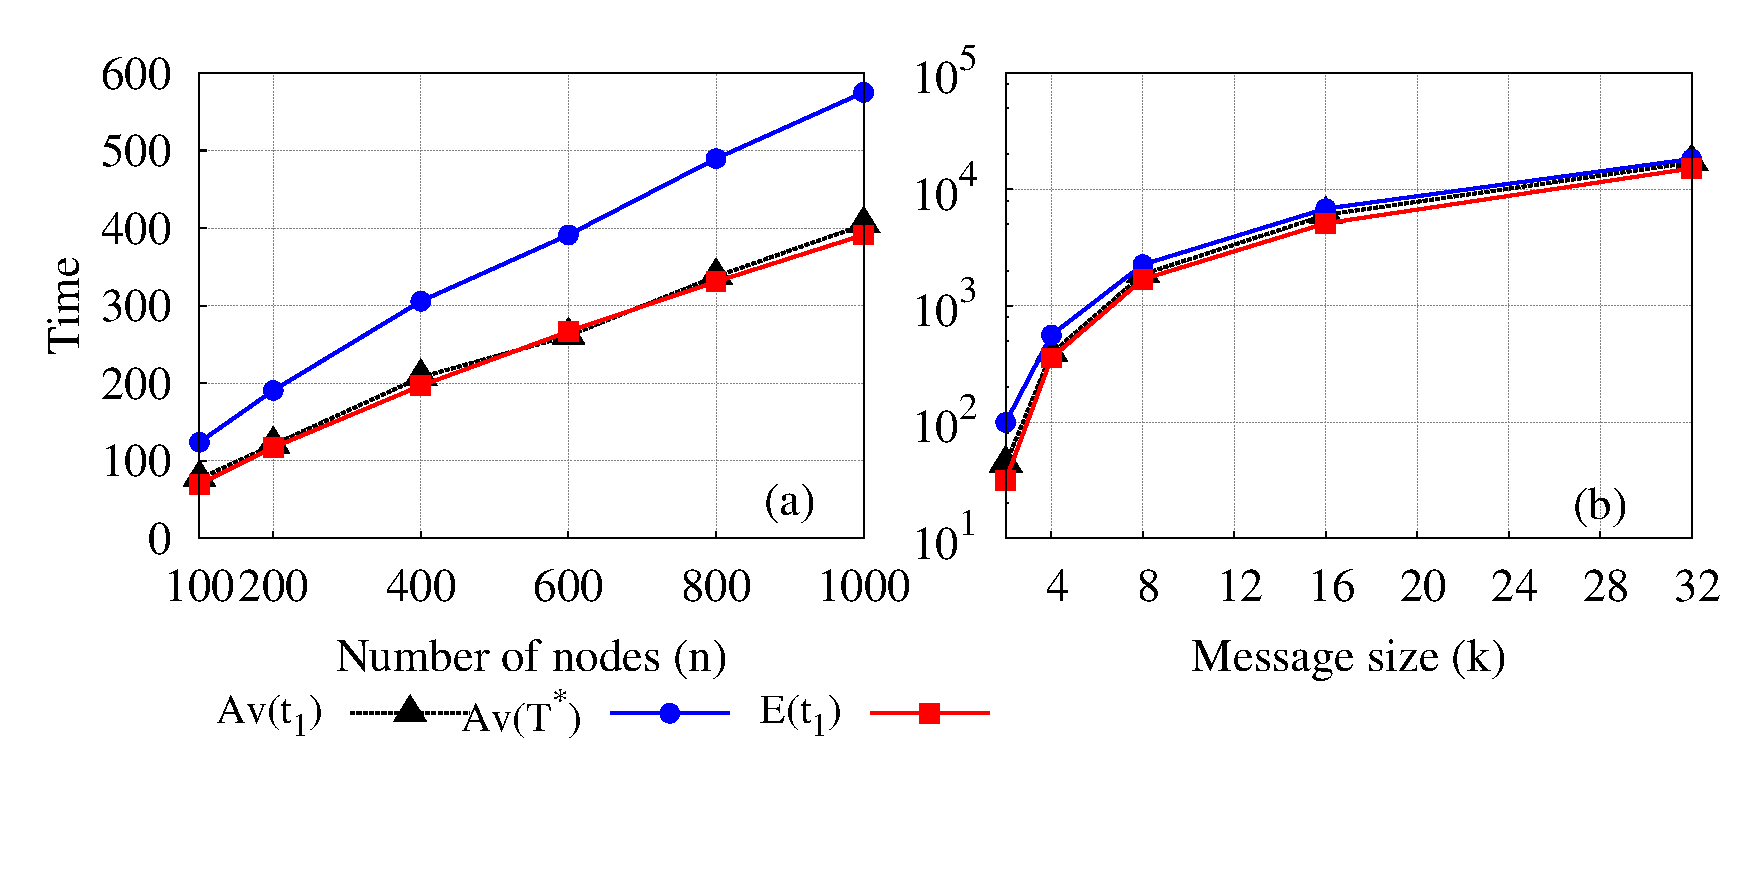
\includegraphics[scale=0.4]{./texfiles/Chapter_3/epl/figs1/plot_var_n_k_complete.eps}
 
 %\vspace{-5mm}
 \caption{$Av(T^*)$ and $Av(t_1)$ versus (a) the number of nodes with message size $k=4$ and (b) $k$ for fixed $d=1000$.
  For both the plots $\hat E(t_1) = C \ast d^{\frac{k-1}{k}}$ where $C = (k!)^{\frac{1}{k}}\Gamma\left(1+\frac{1}{k}\right)$ (refer to theorem \ref{theorem-1}).}
 \label{segSizeVsDelay_nrTrans_varyN_Mall_push_pull}
 %\vspace{-.3cm}
 \end{figure}
% The
% remaining growth is very fast - actually of logarithmic order since several
% new senders in every time step get produced. \vspace{-2mm}

%{\bf E-R Random graphs} - 


\noindent{\em E-R random graph}: We further look into {\bf Erdos-Renyi random graphs}~\cite{erdos1959random} and observe that for sufficiently 
dense graphs (i.e., having high edge probability) the analysis on the complete graph case holds.  
In this regard we first plot $Av(T^{\ast})$ (obtained through simulations) and $\hat{E}(T^{\ast})$ ($n^{\frac{k-1}{k}}$ scaled by a constant, $n$ is the number of nodes) for 
different values of $k$ (message size) (refer to figure \ref{fig_diff_g_n_p}(a)). 
Clearly the theoretical estimate closely follows the simulated result. {As we increase the value of edge probabilities($p$) (i.e., make the network more dense)
 the closer it gets to the theoretical estimate.}
We further plot $Av(T^{\ast})$ (scaled by $\hat{E}(t_{1})$) for varying $p$ in figure \ref{fig_diff_g_n_p}(b). 
The value gets close to 2 with edge probability 1 but remains close to 2 even for lower values of $p$. 
All the results are averaged over $1000$ simulations.



\begin{figure}[htpb]
%\vspace{-.4cm}
\centering
  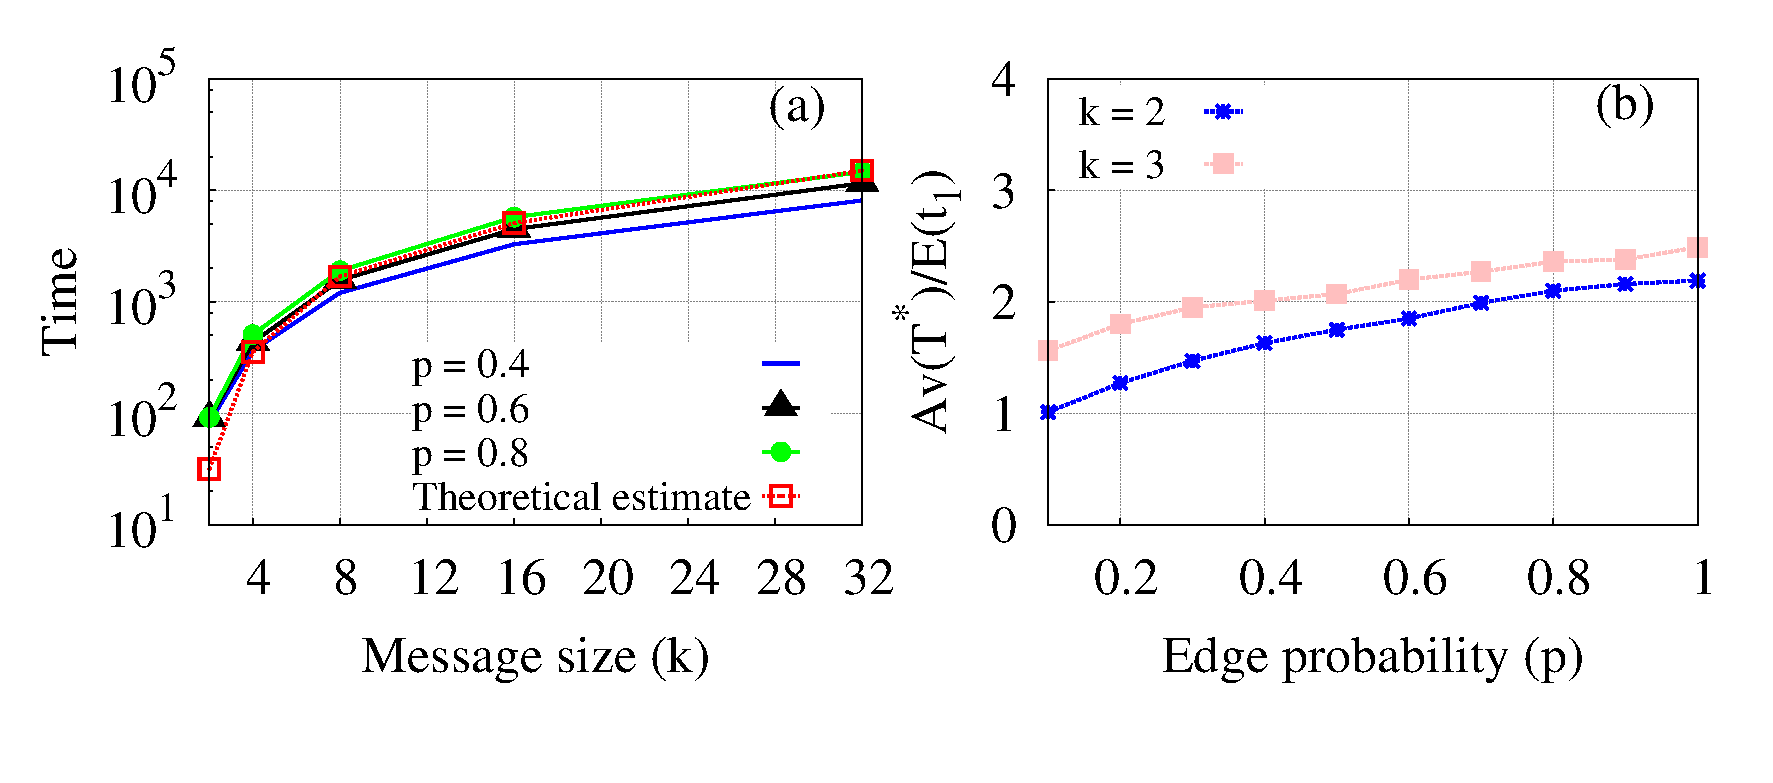
\includegraphics[scale=0.4]{./texfiles/Chapter_3/epl/figs1/ER_graph_result.eps}
  
  %\vspace{-3mm}
  \caption{\label{fig_diff_g_n_p}(a) $Av(T^{\ast})$ and $\hat E(T^{\ast})$ (suitably scaled) for different values of $k$ 
  (b)$Av(T^{\ast})$ versus edge probability in Erdos-Renyi random graph for $k=2$ and $k=3$. In both cases $Av(T^{\ast})$ is normalized by $\hat{E}(t_{1})$ which is $\sqrt{n}$ and $n^{\frac{2}{3}}$ for $k=2$ and $k=3$ respectively.
  \vspace{5mm}}
  %\vspace{-.5cm}
 \end{figure}

%  \begin{figure}[htpb]
%  \centering
%   \includegraphics[scale=0.28]{figs1/tree_ratio.eps}
%   \caption{\label{tree_ratio} ratio of $s_t$ and $s_{t-1}$ throughout the 
% whole duration of the diffusion process for a 5-regular tree }
%  \end{figure} 

\medskip


\noindent
\section{On $d$-regular tree:}
\noindent We next consider the case of {\bf $d$-regular trees} for $d\geq 3$ (at least $2$ children apart from $1$ parent) with a
distinguished root index $0$ which acts as the initial sender. For
simplicity we give the root an out-degree of $(d-1)$ by attaching a virtual
``mother vertex'' to the root which is also a sender but has only one
offspring and is not counted in the estimation of sender nodes (this helps
us avoid handling the initial steps (i.e., when only the root is having the
message) differently from the later steps). Let $A_{l}\left( t\right) ,$ $%
0\leq l<k,$ be the number of nodes on the tree which have exactly $l$
packets at time $t$ and have a direct communication link to one of the
sender nodes at time $t$. Note that each of the so defined nodes has exactly
one connection to a sender node due to the tree structure and the initial
condition of having just one sender at the beginning. We get the following
 exact linear recursion for the expectation $a_{l}\left( t+1\right) :=\hat{%
E}\left( A_{l}\left( t+1\right) \right) $ at time $t+1:$%
\begin{eqnarray*}
\nonumber
a_{l}\left( t+1\right) &=&\frac{d-1}{d}a_{l}\left( t\right) +\frac{1}{d}% 
a_{l-1}\left( t\right) ,1\leq l\leq k-1 \\ \nonumber
a_{0}\left( t+1\right) &=&\frac{d-1}{d}a_{k-1}\left( t\right) +\frac{d-1}{d}%
a_{0}\left( t\right) \nonumber
\end{eqnarray*}%
Note that for the expected number of sender nodes $s_{t}$ at time $t$, we
have 
\begin{equation}
s_{t}=\sum\limits_{t^{\prime }<t}\frac{1}{d}a_{k-1}\left( t^{\prime }\right)
\end{equation}

The asymptotic rate of growth of the variables $\left\{ a_{i}\left( t\right)
\right\} $ as well as $s_{t}$ is entirely determined by the value of the
largest eigenvalue of the associated transition matrix. The maximal
eigenvalue of the associated characteristic polynomial is given by 
\begin{equation*}
\lambda _{\max }=\frac{d-1}{d}+\left( \frac{d-1}{d}\left( \frac{1}{d}\right)
^{k-1}\right) ^{\frac{1}{k}}=\frac{d-1+\left( d-1\right) ^{1/k}}{d}
\end{equation*}


% \begin{figure}[htpb]
% %\vspace{-.5cm}
%  \centering
%   \includegraphics[scale=0.31]{figs1/plot_reg_tree.eps}
%   %\vspace{-5mm}
%   \caption{\label{tree_ratio}(a) Rate of diffusion ($s_t$ - $s_{t-1}$) throughout the 
% whole duration of the diffusion process for a 5-regular tree. (b) Number of nodes at each stage of infection versus time for 
% complete graph of $1000$ nodes with $k=4$. Although the creation of infected nodes is slow initially, the number of partially infected nodes ($0<p<4$) increases rapidly. (inset) Magnified version of the same figure.}
% %\vspace{-.45cm}
%  \end{figure} 

{In figure \ref{fig1}(b) we draw the diffusion dynamics for a 5-regular tree and in the same figure we show that the
analytical estimate (obtained from equation 17) of diffusion rate closely resemble the empirical
observation. 
\if{0}
to the point where the first leaf node receives the full message. 
%At this point, the leaf nodes are the only non-sender nodes in the network which can only be infected by the nodes in the previous level.
Since the leaf nodes after getting infected have no other nodes to infect,  the dynamics
slows down as is evident in the  figure  - the impact of finiteness on 
diffusion conspicuously gets illustrated in figure \ref{tree_ratio}(a)) where we look into the difference of $s_t$ and $s_{t-1}$ throughout the 
whole duration of the diffusion process. We observe that the diffusion rate initially follows an increasing trend and then drops.
\fi
%We observe that the ratio quickly stabilizes to $\lambda_{max}$ (represented in the same figure) after initial few time steps hence supporting our theory.  
%This is followed by a drop in diffusion rate as by that time infection reaches the leaf nodes.}
%\todo{Why should $\lambda_{max}$ = 1, it should be near to 2, check carefully.}

%\noindent {\em d-regular graph}: 
%We further observe that our analytical estimate for $d$-regular trees could be extended for {\bf $d$-regular graph} as well. We
%observe that the analytical estimate closely follows the empirical
%observations as is evident from figure \ref{fig1}. 
\begin{figure}[htpb]
%\vspace{-.5cm}
 \centering
  \includegraphics[scale=0.4]{./texfiles/Chapter_3/epl/figs1/plot_reg_tree.eps}
  %\vspace{-5mm}
  \caption{\label{tree_ratio}(a) $\frac{t_{1}^{\hat p} - t_1}{t_1}$ versus $\bar p$ for a complete graph with $1000$ nodes and $k=4$.
  (b) Number of nodes at each stage of infection versus time for 
complete graph of $1000$ nodes with $k=4$. Although the creation of infected nodes is slow initially, the number of partially infected nodes ($0<l<4$) increases rapidly. 
(inset) Magnified version of the same figure.}
%\vspace{-.45cm}
 \end{figure} 


\medskip


\noindent

\section{Innoculation strategy}
%\label{discussion}

% \begin{figure}[htpb]
%   \centering
%   \includegraphics[scale=0.28]{figs1/plot_var_k.eps}
%   %\includegraphics*[scale=0.28]{figs1/plot_var_k.eps}
%  %\includegraphics*[scale=0.15]{figs/T1_vs_exp_T1_d_reg.eps}
%  
% %\hspace{5mm}(a)\hspace{75mm}(b) 
%  \caption{\label{fig_k} Number of nodes at each stage of infection versus time for complete graph of $1000$ nodes with $k=4$. Although the creation of infected nodes is slow initially, the number of 
%  partially infected nodes ($0<p<4$) increases rapidly.}
% \end{figure}


We have defined the epidemic setting aptly fitting the temporal network system whereby agents remember
interactions from the previous time-steps and only adopt an idea after encountering it multiple times. 
%hence observe that for a system consisting of agents who require persuasion (through multiple contacts) before they adopt an idea, 
We find that such information diffusion process undergoes two phases with a slow initial phase followed by a very fast residual phase. This behavior is observed 
irrespective of the underlying topology (refer to figure~\ref{fig1}, simulations done for scale-free graphs~\cite{barabasi1999emergence} and ER-random graphs).
 The reason behind such behavior is that during the process when the first few nodes get fully infected a large fraction of nodes also simulataneously get partly infected as 
represented in figure \ref{tree_ratio}(b). Once the first set of infected nodes are created these partially infected nodes also get quickly infected and this 
results in a sudden ramp-up in the diffusion rate.

The above observations indicate 
that for such systems spreading could be controlled/contained while the system is still in the slow initial phase. 
Accordingly, we perform an empirical study, whereby, we reduce the level of infection of the agents at one particular time step (say $t$) and then estimate the time required to obtain the first sender vis-a-vis the time $t_1$ when 
such action is not initiated. 
Reduction of infection means removing one packet from the chosen (say with probability $\bar p$)  agent, for example, if an agent has acquired $j$ packets at time $t$, we reduce it to $j$ - 1.  
%(reduce the number of packets by 1) with some predefined probability at a given time during the diffusion process and then estimate $t_1$. 
In specific we considered a complete graph with $1000$ nodes and at $t$ =  $0.5 \ast t_1$  
we reduce the level of infection in each node with a probability ($\bar p$) and measure the corresponding time (say  $t_{1}^{\bar p}$). 
In figure \ref{tree_ratio}(a) we plot $\frac{t_{1}^{\bar p} - t_1}{t_1}$ for different values of $\bar p$. 
We observe that creation of the first sender (other than initiator) i.e.,
beginning of the residual phase (where the rate of spread is increased manifold) could be delayed by almost $20\%$ with a probability of $0.3$. 
We show the experiment by inoculating at one particular time step, however a continuous low-grade innoculation strategy can be
initiated and we believe a threshold can be derived whereby the first sender creation can be pushed to infinity. However that 
can be an interesting research direction to be pursued in the future.

\if{0}
\revision{To further verify our hypothesis we 
performed an empirical study, whereby, we randomly removed a certain fraction of infected nodes and at certain time points and then checked what fraction of the whole population 
got infected after a given period of time. Note that here removal of infected node is same as immunizing them. 
In specific we considered a complete graph with $1000$ nodes and several cases separately in each of which we removed a certain 
fraction of infected nodes ($0.5\%$ of the population ($n$)) at different time instances ($t_{1}, 1.2\ast t_{1}, 1.4 \ast t_{1}\ldots  $) and calculated the total number of 
infected nodes at time $3\ast t_{1}$ (refer to figure \ref{tree_ratio}(a)). At $t_1$ there are only two infected nodes in the system, on removing them the infection does not spread 
at all. In the second case when the infected nodes are removed at $1.2\ast t_1$ the infection spread only to a very small fraction of nodes till $3\ast t_{1}$. 
But removal of infected nodes beyond this point ($1.4\ast T_{1}$) only marginally affected the infection spread. These results indicate that the 
spread of infection could be contained if acted upon during the slow initial phase.}


We believe that our findings could open up paths to a number of future studies especially regulating contagion processes in systems with memory. 
We note that our analysis does not 
consider the fact that the extent of influence decays with time as observed in several real-world diffusion processes. We believe such 
investigation calls for additional research efforts.
\fi
% In subsequent works we plan to provide a detailed analytical estimate for
% the ER-random graphs and the BA-scalefree graphs. In its current form our
% model does not take into consideration the fact that the extent of influence
% decays with time as shown in ~\cite{takaguchi2013bursty}. We plan to
% incorporate this into our model and check how it influences the diffusion
% time given an underlying topology. We would also like to extend our analysis
% to Susceptible-Infected-Recovered (SIR) epidemic spreading models as well.

\medskip





% \acknowledgments
% Marcin Bodych and Tyll Krueger were supported by Indian Institute of Technology Kharagpur, Wroclaw University of Technology and the National Science Centre Poland (NCN) through grant no. 2013/11/B/HS4/01061: Agent based modeling of innovation diffusion.
% 
% \begin{thebibliography}{10}
% \expandafter\ifx\csname url\endcsname\relax\def\url#1{\texttt{#1}}\fi
% 
% \bibitem{anderson1992infectious}
% \Name{Anderson R.~M., May R.~M. \and Anderson B.} \Book{Infectious diseases of
%   humans: dynamics and control} Vol.~28 (Wiley Online Library) 1992.
% 
% \bibitem{watts2002simple}
% \Name{Watts D.~J.} \REVIEW{Proceedings of the National Academy of
%   Sciences}{99}{2002}{5766}.
% 
% \bibitem{dodds2004universal}
% \Name{Dodds P.~S. \and Watts D.~J.} \REVIEW{Physical review
%   letters}{92}{2004}{218701}.
% 
% \bibitem{pnas1}
% \Name{Kramer A.~D., Guillory J.~E. \and Hancock J.~T.} \REVIEW{Proceedings of
%   the National Academy of Sciences}{111}{2014}{8788}.
% 
% \bibitem{pnas2}
% \Name{Aral S., Muchnik L. \and Sundararajan A.} \REVIEW{Proceedings of the
%   National Academy of Sciences}{106}{2009}{21544}.
% 
% \bibitem{tang2009epidemic}
% \Name{Tang M., Liu Z. \and Li B.} \REVIEW{EPL (Europhysics
%   Letters)}{87}{2009}{18005}.
% 
% \bibitem{son2012percolation}
% \Name{Son S.-W., Bizhani G., Christensen C., Grassberger P. \and Paczuski M.}
%   \REVIEW{EPL (Europhysics Letters)}{97}{2012}{16006}.
% 
% \bibitem{takaguchi2013bursty}
% \Name{Takaguchi T., Masuda N. \and Holme P.} \REVIEW{PloS
%   one}{8}{2013}{e68629}.
% 
% \bibitem{karsai2011small}
% \Name{Karsai M., Kivel{\"a} M., Pan R.~K., Kaski K., Kert{\'e}sz J.,
%   Barab{\'a}si A.-L. \and Saram{\"a}ki J.} \REVIEW{Physical Review
%   E}{83}{2011}{025102}.
% 
% \bibitem{karimi2013threshold}
% \Name{Karimi F. \and Holme P.} \REVIEW{Physica A: Statistical Mechanics and its
%   Applications}{392}{2013}{3476}.
% 
% \bibitem{backlund2014effects}
% \Name{Backlund V.-P., Saram{\"a}ki J. \and Pan R.~K.} \REVIEW{Physical Review
%   E}{89}{2014}{062815}.
% 
% \bibitem{rocha2013bursts}
% \Name{Rocha L.~E. \and Blondel V.~D.} \REVIEW{PLoS Comput
%   Biol}{9}{2013}{e1002974}.
% 
% \bibitem{masuda2013predicting}
% \Name{Masuda N. \and Holme P.} \REVIEW{F1000 prime reports}{5}{2013}{6}.
% 
% \bibitem{prl1}
% \Name{Bogu{\~n}{\'a} M., Castellano C. \and Pastor-Satorras R.}
%   \REVIEW{Physical review letters}{111}{2013}{068701}.
% 
% \bibitem{van2012epidemic}
% \Name{Van~Mieghem P.} \REVIEW{EPL (Europhysics Letters)}{97}{2012}{48004}.
% 
% \bibitem{zhang2014susceptible}
% \Name{Zhang Y.-Q. \and Li X.} \REVIEW{EPL (Europhysics
%   Letters)}{108}{2014}{28006}.
% 
% \bibitem{joh2009dynamics}
% \Name{Joh R.~I., Wang H., Weiss H. \and Weitz J.~S.} \REVIEW{Bulletin of
%   mathematical biology}{71}{2009}{845}.
% 
% \bibitem{sanghavi2007gossiping}
% \Name{Sanghavi S., Hajek B. \and Massouli{\'e} L.} \REVIEW{IEEE Transactions on
%   Information Theory}{53}{2007}{4640}.
% 
% \bibitem{qiu2004modeling}
% \Name{Qiu D. \and Srikant R.} \Book{Modeling and performance analysis of
%   bittorrent-like peer-to-peer networks} in proc. of \Book{ACM SIGCOMM computer
%   communication review} Vol.~34 (ACM) 2004 pp. 367--378.
% 
% \bibitem{romero2011differences}
% \Name{Romero D.~M., Meeder B. \and Kleinberg J.} \Book{Differences in the
%   mechanics of information diffusion across topics: idioms, political hashtags,
%   and complex contagion on twitter} in proc. of \Book{Proceedings of the 20th
%   international conference on World wide web} (ACM) 2011 pp. 695--704.
% 
% \bibitem{granovetter1978threshold}
% \Name{Granovetter M.} \REVIEW{American journal of sociology}{}{1978}{1420}.
% 
% \bibitem{sur1}
% \Name{Mollison D.} \Book{Epidemic models: their structure and relation to data}
%   Vol.~5 (Cambridge University Press) 1995.
% 
% \bibitem{volz2007susceptible}
% \Name{Volz E. \and Meyers L.~A.} \REVIEW{Proceedings of the Royal Society of
%   London B: Biological Sciences}{274}{2007}{2925}.
% 
% \bibitem{kaplan1977generalization}
% \Name{Kaplan N.} \REVIEW{Journal of Applied Probability}{}{1977}{212}.
% 
% \bibitem{wald}
% \Name{Wald A.} \REVIEW{The Annals of Mathematical Statistics}{15}{1944}{283}.
% 
% \bibitem{erdos1959random}
% \Name{Erd{\"o}s P. \and R{\'e}nyi A.} \REVIEW{Publicationes Mathematicae
%   (Debrecen)}{6}{1959}{290}.
% 
% \bibitem{barabasi1999emergence}
% \Name{Barab{\'a}si A.-L. \and Albert R.} \REVIEW{science}{286}{1999}{509}.
% 
% \end{thebibliography}
% 
% 
% \end{document}



%% bare_conf.tex
%% V1.3
%% 2007/01/11
%% by Michael Shell
%% See:
%% http://www.michaelshell.org/
%% for current contact information.
%%
%% This is a skeleton file demonstrating the use of IEEEtran.cls
%% (requires IEEEtran.cls version 1.7 or later) with an IEEE conference paper.
%%
%% Support sites:
%% http://www.michaelshell.org/tex/ieeetran/
%% http://www.ctan.org/tex-archive/macros/latex/contrib/IEEEtran/
%% and
%% http://www.ieee.org/

%%*************************************************************************
%% Legal Notice:
%% This code is offered as-is without any warranty either expressed or
%% implied; without even the implied warranty of MERCHANTABILITY or
%% FITNESS FOR A PARTICULAR PURPOSE! 
%% User assumes all risk.
%% In no event shall IEEE or any contributor to this code be liable for
%% any damages or losses, including, but not limited to, incidental,
%% consequential, or any other damages, resulting from the use or misuse
%% of any information contained here.
%%
%% All comments are the opinions of their respective authors and are not
%% necessarily endorsed by the IEEE.
%%
%% This work is distributed under the LaTeX Project Public License (LPPL)
%% ( http://www.latex-project.org/ ) version 1.3, and may be freely used,
%% distributed and modified. A copy of the LPPL, version 1.3, is included
%% in the base LaTeX documentation of all distributions of LaTeX released
%% 2003/12/01 or later.
%% Retain all contribution notices and credits.
%% ** Modified files should be clearly indicated as such, including  **
%% ** renaming them and changing author support contact information. **
%%
%% File list of work: IEEEtran.cls, IEEEtran_HOWTO.pdf, bare_adv.tex,
%%                    bare_conf.tex, bare_jrnl.tex, bare_jrnl_compsoc.tex
%%*************************************************************************

% *** Authors should verify (and, if needed, correct) their LaTeX system  ***
% *** with the testflow diagnostic prior to trusting their LaTeX platform ***
% *** with production work. IEEE's font choices can trigger bugs that do  ***
% *** not appear when using other class files.                            ***
% The testflow support page is at:
% http://www.michaelshell.org/tex/testflow/



% Note that the a4paper option is mainly intended so that authors in
% countries using A4 can easily print to A4 and see how their papers will
% look in print - the typesetting of the document will not typically be
% affected with changes in paper size (but the bottom and side margins will).
% Use the testflow package mentioned above to verify correct handling of
% both paper sizes by the user's LaTeX system.
%
% Also note that the "draftcls" or "draftclsnofoot", not "draft", option
% should be used if it is desired that the figures are to be displayed in
% draft mode.
%
% \documentclass[10pt, conference, letterpaper]{IEEEtran}
% \usepackage{amssymb}
% \usepackage{amstext}
% \usepackage{amsmath}
% %\usepackage{commonTemplates/algorithm}
% %\usepackage{commonTemplates/algorithmic}
% \usepackage{commonTemplates/subfigure}
% \usepackage{commonTemplates/graphicx}
% \usepackage{commonTemplates/graphics}
% \usepackage{commonTemplates/multirow}
% \usepackage[]{algorithm2e}
% \usepackage{color}
% %\usepackage{vmargin}
% %\usepackage[letter]{geometry}
% \special{papersize=8.5in,11in}
% \newtheorem{theorem}{Theorem}
% \newtheorem{acknowledgement}[theorem]{Acknowledgement}
% %\newtheorem{algorithm}[theorem]{Algorithm}
% \newtheorem{axiom}[theorem]{Axiom}
% \newtheorem{case}[theorem]{Case}
% \newtheorem{claim}[theorem]{Claim}
% \newtheorem{conclusion}[theorem]{Conclusion}
% \newtheorem{condition}[theorem]{Condition}
% \newtheorem{conjecture}[theorem]{Conjecture}
% \newtheorem{corollary}[theorem]{Corollary}
% \newtheorem{criterion}[theorem]{Criterion}
% \newtheorem{definition}[theorem]{Definition}
% \newtheorem{example}[theorem]{Example}
% \newtheorem{exercise}[theorem]{Exercise}
% \newtheorem{lemma}[theorem]{Lemma}
% \newtheorem{notation}[theorem]{Notation}
% \newtheorem{problem}[theorem]{Problem}
% \newtheorem{proposition}[theorem]{Proposition}
% \newtheorem{remark}[theorem]{Remark}
% \newtheorem{solution}[theorem]{Solution}
% \newtheorem{summary}[theorem]{Summary}
% \newcommand{\todo}[1]{\textcolor{red}{\textbf{{NILOY: #1}}}}

%
%\ifCLASSINFOpdf
  % \usepackage[pdftex]{graphicx}
  % declare the path(s) where your graphic files are
  % \graphicspath{{../pdf/}{../jpeg/}}
  % and their extensions so you won't have to specify these with
  % every instance of \includegraphics
  % \DeclareGraphicsExtensions{.pdf,.jpeg,.png}
%\else
  % or other class option (dvipsone, dvipdf, if not using dvips). graphicx
  % will default to the driver specified in the system graphics.cfg if no
  % driver is specified.
  % \usepackage[dvips]{graphicx}
  % declare the path(s) where your graphic files are
  % \graphicspath{{../eps/}}
  % and their extensions so you won't have to specify these with
  % every instance of \includegraphics
  % \DeclareGraphicsExtensions{.eps}
%\fi
% graphicx was written by David Carlisle and Sebastian Rahtz. It is
% required if you want graphics, photos, etc. graphicx.sty is already
% installed on most LaTeX systems. The latest version and documentation can
% be obtained at: 
% http://www.ctan.org/tex-archive/macros/latex/required/graphics/
% Another good source of documentation is "Using Imported Graphics in
% LaTeX2e" by Keith Reckdahl which can be found as epslatex.ps or
% epslatex.pdf at: http://www.ctan.org/tex-archive/info/
%
% latex, and pdflatex in dvi mode, support graphics in encapsulated
% postscript (.eps) format. pdflatex in pdf mode supports graphics
% in .pdf, .jpeg, .png and .mps (metapost) formats. Users should ensure
% that all non-photo figures use a vector format (.eps, .pdf, .mps) and
% not a bitmapped formats (.jpeg, .png). IEEE frowns on bitmapped formats
% which can result in "jaggedy"/blurry rendering of lines and letters as
% well as large increases in file sizes.
%
% You can find documentation about the pdfTeX application at:
% http://www.tug.org/applications/pdftex





% *** MATH PACKAGES ***
%
%\usepackage[cmex10]{amsmath}
% A popular package from the American Mathematical Society that provides
% many useful and powerful commands for dealing with mathematics. If using
% it, be sure to load this package with the cmex10 option to ensure that
% only type 1 fonts will utilized at all point sizes. Without this option,
% it is possible that some math symbols, particularly those within
% footnotes, will be rendered in bitmap form which will result in a
% document that can not be IEEE Xplore compliant!
%
% Also, note that the amsmath package sets \interdisplaylinepenalty to 10000
% thus preventing page breaks from occurring within multiline equations. Use:
%\interdisplaylinepenalty=2500
% after loading amsmath to restore such page breaks as IEEEtran.cls normally
% does. amsmath.sty is already installed on most LaTeX systems. The latest
% version and documentation can be obtained at:
% http://www.ctan.org/tex-archive/macros/latex/required/amslatex/math/





% *** SPECIALIZED LIST PACKAGES ***
%
%\usepackage{algorithmic}
% algorithmic.sty was written by Peter Williams and Rogerio Brito.
% This package provides an algorithmic environment fo describing algorithms.
% You can use the algorithmic environment in-text or within a figure
% environment to provide for a floating algorithm. Do NOT use the algorithm
% floating environment provided by algorithm.sty (by the same authors) or
% algorithm2e.sty (by Christophe Fiorio) as IEEE does not use dedicated
% algorithm float types and packages that provide these will not provide
% correct IEEE style captions. The latest version and documentation of
% algorithmic.sty can be obtained at:
% http://www.ctan.org/tex-archive/macros/latex/contrib/algorithms/
% There is also a support site at:
% http://algorithms.berlios.de/index.html
% Also of interest may be the (relatively newer and more customizable)
% algorithmicx.sty package by Szasz Janos:
% http://www.ctan.org/tex-archive/macros/latex/contrib/algorithmicx/




% *** ALIGNMENT PACKAGES ***
%
%\usepackage{array}
% Frank Mittelbach's and David Carlisle's array.sty patches and improves
% the standard LaTeX2e array and tabular environments to provide better
% appearance and additional user controls. As the default LaTeX2e table
% generation code is lacking to the point of almost being broken with
% respect to the quality of the end results, all users are strongly
% advised to use an enhanced (at the very least that provided by array.sty)
% set of table tools. array.sty is already installed on most systems. The
% latest version and documentation can be obtained at:
% http://www.ctan.org/tex-archive/macros/latex/required/tools/


%\usepackage{mdwmath}
%\usepackage{mdwtab}
% Also highly recommended is Mark Wooding's extremely powerful MDW tools,
% especially mdwmath.sty and mdwtab.sty which are used to format equations
% and tables, respectively. The MDWtools set is already installed on most
% LaTeX systems. The lastest version and documentation is available at:
% http://www.ctan.org/tex-archive/macros/latex/contrib/mdwtools/


% IEEEtran contains the IEEEeqnarray family of commands that can be used to
% generate multiline equations as well as matrices, tables, etc., of high
% quality.


%\usepackage{eqparbox}
% Also of notable interest is Scott Pakin's eqparbox package for creating
% (automatically sized) equal width boxes - aka "natural width parboxes".
% Available at:
% http://www.ctan.org/tex-archive/macros/latex/contrib/eqparbox/





% *** SUBFIGURE PACKAGES ***
%\usepackage[tight,footnotesize]{subfigure}
% subfigure.sty was written by Steven Douglas Cochran. This package makes it
% easy to put subfigures in your figures. e.g., "Figure 1a and 1b". For IEEE
% work, it is a good idea to load it with the tight package option to reduce
% the amount of white space around the subfigures. subfigure.sty is already
% installed on most LaTeX systems. The latest version and documentation can
% be obtained at:
% http://www.ctan.org/tex-archive/obsolete/macros/latex/contrib/subfigure/
% subfigure.sty has been superceeded by subfig.sty.



%\usepackage[caption=false]{caption}
%\usepackage[font=footnotesize]{subfig}
% subfig.sty, also written by Steven Douglas Cochran, is the modern
% replacement for subfigure.sty. However, subfig.sty requires and
% automatically loads Axel Sommerfeldt's caption.sty which will override
% IEEEtran.cls handling of captions and this will result in nonIEEE style
% figure/table captions. To prevent this problem, be sure and preload
% caption.sty with its "caption=false" package option. This is will preserve
% IEEEtran.cls handing of captions. Version 1.3 (2005/06/28) and later 
% (recommended due to many improvements over 1.2) of subfig.sty supports
% the caption=false option directly:
%\usepackage[caption=false,font=footnotesize]{subfig}
%
% The latest version and documentation can be obtained at:
% http://www.ctan.org/tex-archive/macros/latex/contrib/subfig/
% The latest version and documentation of caption.sty can be obtained at:
% http://www.ctan.org/tex-archive/macros/latex/contrib/caption/




% *** FLOAT PACKAGES ***
%
%\usepackage{fixltx2e}
% fixltx2e, the successor to the earlier fix2col.sty, was written by
% Frank Mittelbach and David Carlisle. This package corrects a few problems
% in the LaTeX2e kernel, the most notable of which is that in current
% LaTeX2e releases, the ordering of single and double column floats is not
% guaranteed to be preserved. Thus, an unpatched LaTeX2e can allow a
% single column figure to be placed prior to an earlier double column
% figure. The latest version and documentation can be found at:
% http://www.ctan.org/tex-archive/macros/latex/base/



%\usepackage{stfloats}
% stfloats.sty was written by Sigitas Tolusis. This package gives LaTeX2e
% the ability to do double column floats at the bottom of the page as well
% as the top. (e.g., "\begin{figure*}[!b]" is not normally possible in
% LaTeX2e). It also provides a command:
%\fnbelowfloat
% to enable the placement of footnotes below bottom floats (the standard
% LaTeX2e kernel puts them above bottom floats). This is an invasive package
% which rewrites many portions of the LaTeX2e float routines. It may not work
% with other packages that modify the LaTeX2e float routines. The latest
% version and documentation can be obtained at:
% http://www.ctan.org/tex-archive/macros/latex/contrib/sttools/
% Documentation is contained in the stfloats.sty comments as well as in the
% presfull.pdf file. Do not use the stfloats baselinefloat ability as IEEE
% does not allow \baselineskip to stretch. Authors submitting work to the
% IEEE should note that IEEE rarely uses double column equations and
% that authors should try to avoid such use. Do not be tempted to use the
% cuted.sty or midfloat.sty packages (also by Sigitas Tolusis) as IEEE does
% not format its papers in such ways.





% *** PDF, URL AND HYPERLINK PACKAGES ***
%
%\usepackage{url}
% url.sty was written by Donald Arseneau. It provides better support for
% handling and breaking URLs. url.sty is already installed on most LaTeX
% systems. The latest version can be obtained at:
% http://www.ctan.org/tex-archive/macros/latex/contrib/misc/
% Read the url.sty source comments for usage information. Basically,
% \url{my_url_here}.





% *** Do not adjust lengths that control margins, column widths, etc. ***
% *** Do not use packages that alter fonts (such as pslatex).         ***
% There should be no need to do such things with IEEEtran.cls V1.6 and later.
% (Unless specifically asked to do so by the journal or conference you plan
% to submit to, of course. )


% correct bad hyphenation here
% \hyphenation{op-tical net-works semi-conduc-tor}
% 
% 
% \begin{document}
% %
% % paper title
% % can use linebreaks \\ within to get better formatting as desired
% \title{On the broadcast of segmented messages \\ in dynamic networks}


% author names and affiliations
% use a multiple column layout for up to three different
% affiliations


% \author{\IEEEauthorblockN{Michael Shell}
% \IEEEauthorblockA{School of Electrical and\\Computer Engineering\\
% Georgia Institute of Technology\\
% Atlanta, Georgia 30332--0250\\
% Email: http://www.michaelshell.org/contact.html}
% \and
% \IEEEauthorblockN{Homer Simpson}
% \IEEEauthorblockA{Twentieth Century Fox\\
% Springfield, USA\\
% Email: homer@thesimpsons.com}
% \and
% \IEEEauthorblockN{James Kirk\\ and Montgomery Scott}
% \IEEEauthorblockA{Starfleet Academy\\
% San Francisco, California 96678-2391\\
% Telephone: (800) 555--1212\\
% Fax: (888) 555--1212}}

% conference papers do not typically use \thanks and this command
% is locked out in conference mode. If really needed, such as for
% the acknowledgment of grants, issue a \IEEEoverridecommandlockouts
% after \documentclass

% for over three affiliations, or if they all won't fit within the width
% of the page, use this alternative format:
% 
% \author{\IEEEauthorblockN{Sandipan Sikdar\IEEEauthorrefmark{1},
% Marcin Bodych\IEEEauthorrefmark{2},
% Rajib Ranjan Maiti\IEEEauthorrefmark{3},
% Biswajit Paria\IEEEauthorrefmark{1}\\
% Niloy Ganguly\IEEEauthorrefmark{1},
% Tyll Krueger\IEEEauthorrefmark{2}
% Animesh Mukherjee\IEEEauthorrefmark{1}}
% \IEEEauthorblockA{\IEEEauthorrefmark{1}Indian Institute of Technology Kharagpur, Kharagpur, India
% }
% \IEEEauthorblockA{\IEEEauthorrefmark{2}Wroclaw University of Technology, Wroclaw, Poland}
% \IEEEauthorblockA{\IEEEauthorrefmark{3}Instituto di Informatica e Telematica, Pisa, Italy\\
% }}




% use for special paper notices
%\IEEEspecialpapernotice{(Invited Paper)}




% make the title area
% \maketitle
% 
% %\vspace{-5cm}
% \begin{abstract}
% %\boldmath
% %\input{Infocom2015_abstract}
% In the era of big data, graph sampling is inevitable in many settings. Existing sampling methods are mostly designed for static graphs, and aim to preserve {\em major} structural properties of the original graph  (such as degree distribution, clustering coefficient etc.) in the sample. We posit that for any sampling method it is impossible to produce universal representative which can preserve {\em all} the properties of the original graph; rather sampling should be application specific (such as preserving hubs for information diffusion). Here we consider {\em community detection} as an application and  propose \compas, a novel sampling strategy that unlike previous methods, is not only designed for {\em streaming graphs} (which is more realistic representation of a graph) 
but also {\em preserves the community structure} of the original graph in the sample. \compas~interweaves graph sampling and community detection in such a way that each gets benefits from the other to produce a community-preserved sample as well as its associated community structure (as a bi-product). 
%These generated sample may be viewed as stratified sample in that it consists of members from most or all communities in the original graph.

Empirical results on both synthetic and different real-world graphs show that \compas~is the best to preserve the underlying community structure and quite competitive in maintaining general graph properties with average performance reaching 85.5\% of the most informed algorithm on static graphs.
Finally, we present additional benefits of \compas~through two applications -- selection of right community detection algorithm for a particular graph 
%message spreading in streaming graphs 
and selection of training set for online learning. For both the applications \compas~ performs almost as good as the most informed baseline for static graphs. 
%We obtain a performance that is within {\color{red} y\% of} the most informed algorithm available for static graphs.%\TODO{Report improvements here again.} 



% \end{abstract}
% IEEEtran.cls defaults to using nonbold math in the Abstract.
% This preserves the distinction between vectors and scalars. However,
% if the conference you are submitting to favors bold math in the abstract,
% then you can use LaTeX's standard command \boldmath at the very start
% of the abstract to achieve this. Many IEEE journals/conferences frown on
% math in the abstract anyway.

% no keywords




% For peer review papers, you can put extra information on the cover
% page as needed:
% \ifCLASSOPTIONpeerreview
% \begin{center} \bfseries EDICS Category: 3-BBND \end{center}
% \fi
%
% For peerreview papers, this IEEEtran command inserts a page break and
% creates the second title. It will be ignored for other modes.
% \IEEEpeerreviewmaketitle
% 
% 
% \vspace{-3mm}
%\section{Introduction}
%\vspace{-1.5mm}
                                                                                                                                                                                                                                                                                                                                                                                                                                                                                                     
%\noindent
{\bf Broadcast algorithm based on diffusion model:} The study of broadcast over unstructured and mobile networks always assumes that the 
size of the message is  small enough to be transfered from one node to other 
on the short durations of contacts between the nodes. 
Contrary to this, we here explore
 the idea of ``segmented messages'' where we assume that the duration of a contact 
between the nodes is not always sufficient for the transfer and therefore the message might need to be 
segmented/divided into sub-parts and sent individually. 
At the ethernet level such techniques of segmented broadcast are often termed as pipelined broadcast 
~\cite{patarasuk2008techniques, watts1995pipelined}. Note that this is equivalent to diffusion model we proposed earlier with number of contacts ($k$) replaced by number 
of packets in a message. 
We systematically study the effect of the size and partition structure of the message on the broadcast time.
 %considering different variants of the basic push-pull transfer protocol. 
% \textcolor{red}{Note that we essentially deal with a theoretical abstraction of the problem of segmented message spreading and show that it is 
% significantly different from the classical epidemic spreading.}{\bf we have not shown this.} \todo{Have we shown this?}
%The transmission algorithms that we propose might require suitable adjustments when it is adapted for a specific type of a dynamic network.      

%\todo{The two paragraphs need to be discussed, n, m, k, s are extremely confusing and need to be simplified}
{In specific, we investigate in details the effect of message segmentation as well as the message transfer protocols on the overall 
broadcast delay and message wastage. 
We assume that a big file is split into $k$ ($>1$) packets and 
%the packets are grouped into $s$ ($\geq 1$) segments, each containing $k$ packets. 
at the beginning, there is only one sender node in the network that has all the packets. 
Further, a node can transfer only one  packet in a single contact opportunity, and it can do so only when it has received all the 
packets constituting at least one segment of the message. When all the nodes present in the network have eventually received all the packets, 
broadcasting is assumed to be complete. 

Initially, we investigate the push transfer protocol whereby messages are `pushed'
by the node holding a message to the node not having the message ~\cite{demers1987epidemic,lo2008some}. 
We attempt to study the effect in different types of topologies e.g., complete graph, $d$-regular tree, $d$-regular graph, random graph (with average degree $d$). 
%For a complete graph topology of size $n$ and the simple push case  
%we show that the overall time required for the broadcast in case of segmented messages scales as $n^{\frac{k-1}{k}}$ where $k>1$ is the number of packets. 
%This is in sharp contrast to the single message case ($k$ = $1$) where it has been shown that broadcasting time 
%scales as $\log{(n)}$ ~\cite{rumarSreadingPushPull,rumourSpreading_evolvingGraph_PushPull}. 
A remarkable observation is that in topologies like $d$ regular tree, $d$ regular graph and random graph,
for even the simple push transfer protocol, one can find an optimal value of $d (d>1)$, for which the broadcast delay and wastage is minimum. (section ~\ref{suggestions}).
As a corollary, through simulations on real traces, we identify that for two networks with the same number of nodes, broadcast 
time required is far smaller for the one with lesser edge density. 
%On removing some edges from the original network while maintaining the network connectivity 
%substantially reduces the broadcast time.
This finding, 
we believe, indicates a very crucial point -- a sparse communication network per se is not disadvantageous. 

However, we observe that push transfer protocol results in a large number of useless contacts.  
%In order to reduce the same, we propose in this paper, a ``give-up'' mechanism whereby nodes attempt to discover 
%their neighborhood by maintaining a history of all previous contacts and stop attempting to perform any further 
%push after a certain number of unique unsuccessful contacts (reduces to 10\%, message size = 2). 
An unsuccessful/useless contact here refers to a case 
where a sender node attempts to send a packet to another node who already has the packet. 
In order to reduce both broadcast time and wastage we propose a combined strategy whereby the nodes in the system initially push and then switch over 
to pull after a certain percentage (say $x$) of the nodes have received the full message. We observe that if $x$ is carefully chosen, both gain in  
broadcast time and reduction in wastage is achieved. However, to determine that $x$\% of the nodes have indeed received the message, the system needs to maintain a global information 
which is not feasible in a distributed setting like this.
% An unsuccessful/useless contact here refers to a case 
% where a sender node attempts to send a packet to another node who already has the packet. 
% Nevertheless, such a ``give-up'' strategy results in drastic reduction in the number of nodes 
% finally receiving the message especially for larger values of $m$ (55\%, message size = 16). 
In order to circumvent this problem, we introduce a distributed version of the previous technique along with ``give-up'' mechanism 
whereby nodes attempt to discover 
their neighborhood by maintaining a history of all previous contacts and stops participating in the broadcast 
after a certain number of unique unsuccessful contacts.  
This algorithm when tested over Gnutella topologies is found to yield  lesser broadcast delay 
without significant increase in wastage.
We believe, our algorithm with minor modifications is applicable to a 
wide range of dynamic networks ~\cite{eugster2003many,jin2010epidemic,sanghavi2007gossiping}.



\medskip

%\vspace{-2mm}
\section{Broadcast algorithm based on the diffusion model}
\label{algorithm_outline}
%\vspace{-2mm}
\noindent
%\section{Broadcast algorithm based on the diffusion model}
We now proceed to propose a broadcast algorithm based on the information diffusion model proposed earlier. 
Note that contrary to the general assumption that size of a message is small enough to be transferred from one node to other 
on the short durations of contacts between the nodes, we consider a more stringent case that is, the duration of a contact 
between the nodes is not always sufficient for the transfer and therefore the message might need to be 
segmented/divided into sub-parts and sent individually. Further note that our proposed diffusion model is a natural fit (which we elaborate on next) as the 
number of contacts to contract infection can be replaced by the number of sub-parts in the message. 

%\vspace{-3.5mm}
\subsection{Agent configuration and network setup}
%\vspace{-2mm}
We consider a network topology $G = < V,E >$ where each node in $V$ represents an agent of the network and any link in $E$ represents a contact 
opportunity between a pair of nodes (agents) in the whole time span through which the network is active. So for any node (agent) $n_{i}$ in this network, its one hop 
neighbors are the nodes (agents) which are within the connection proximity of $n_{i}$ and at each time step $n_{i}$ at random can connect to any one of them. 


\subsection{Message configuration}
%\vspace{-2mm}
We consider that a message $\mathcal{M}$ is divided into a set of $m$ packets, i.e., $|\mathcal{M}| = m$. 
 Packets in $\mathcal{M}$ are grouped into a set $\mathcal{S}$ of $s$ segments, 
where each segment consists of $k = m/s$ packets (i.e., $s$ can take only those values for which $m \bmod s = 0$). 
For instance, if $\mathcal{M}$ constitutes of 4 packets and 2 segments then each of the segment is composed of 2 packets. 
%Note that we will mostly consider that there is only a single segment in the message ($m=k$) unless specified otherwise.

%\vspace{-5.9mm}
\subsection{Transfer protocol}
%\vspace{-2mm}
In this framework, transfer of a message during a contact refers to the transfer of one single packet of any segment of a message. 
Transfer of a packet from $u_i$ to $v_j$ during a contact can take place only 
when $u_i$ qualifies as a {\em sender} by having all the packets of at least one of the message segments. 
The two basic modes of message transfer that we consider are the push and the (restricted) pull epidemic. 

%\begin{itemize}
 %\vspace{-2mm}
 \noindent \emph{Push technique:} 
  \begin{itemize}
 % \vspace{-3mm}
   \item \emph{Step 1:} At any time step, $u_i$ (already a sender) establishes a communication link with $v_j$, 
   from its neighborhood and finds an exclusive set of packets that $u_i$ has but $v_j$ does not have in its buffer. 
   \item \emph{Step 2:} If $u_i$ can find such a (non-empty) set, then it transfers only one packet from this set to $v_j$. 
  \end{itemize}
  %Note that the \emph{push} technique is exactly similar to the diffusion model proposed earlier.
%\vspace{-2mm}
 \noindent \emph{Pull technique:} 
% \vspace{-3mm}
 \begin{itemize}
  \item \emph{Step 1:} At any time step between $v_j$ and $u_i$, $v_j$ establishes a communication link with $u_i$ 
  and requests for a packet that it has not received yet. 
  \item \emph{Step 2:} Given that $u_i$ has already become a sender it first finds such a packet from its own buffer and then transfers a copy of it to $v_j$.
 \end{itemize}
  Note that in the traditional pull technique, $u_i$, being a sender, may transfer more than one packet if it gets multiple simultaneous requests from more than one agent at any particular time step. However, unlike the traditional case, here $u_i$ can serve only one request in case there are multiple pull requests. Such a restriction actually allows for conservation of both battery power and network bandwidth in resource constrained scenarios like DTN. 
 Also note that we consider the duration of each communication link is long enough for the transfer of at least a single packet.  


%\vspace{-5mm}
\subsection{Metrics of interest}
%\vspace{-2mm}
We are interested to evaluate the performance of a broadcast protocol in terms of two different metrics. The first metric concerns broadcast delay. 
The second metric centers around a complementary issue of power and bandwidth consumption.
\begin{itemize}
%\vspace{-4mm}
 \item \textbf{Broadcast delay $T^*$} - this is the time from the point when the message source starts sending the first packet to the point when all the agents in the network have received the entire message. 
 $E(T^*)$ denotes the expected broadcast time. 
 In addition, we are also interested in the time $T_i$ which is the minimum time at which there are $i$ senders (except the source) in the network, and especially in $T_1$ since, as we shall see, that this is the prime determinant of the entire broadcast time. 
 %\todo{why are these lines needed - Finally, note that $T^*$ may not correspond to $T_{n-1}$, i.e., the time when there are $n-1$ senders (except the source) in the network because all $n-1$ agents need not become senders to spread the message.}  
 \item \textbf{Broadcast wastage $C_m^*$} - let $C_l$ and $C_p$ be the total number of communication links that get established in the network and the total number of successful packet transfers respectively. We define the broadcast wastage as $C_m^* = (C_l - C_p)/C_l$. This metric essentially measures the number of useless contacts in the network during which no packet could be transferred and is therefore a direct cause of energy wastage.
\end{itemize}

\subsection{Broadcast algorithms}
We consider following four algorithms for broadcasting messages. While the first one (Blind Push) is exactly similar to the diffusion model proposed earlier, the others 
builds on it.
\subsubsection{Blind push (B-P)}
{
An initiator node is the one which has the full message in the beginning. At each time step all the nodes 
in the system having the full message communicate with a node in their proximity and try to $push$. 
%If it is successful then a unit bandwidth is consumed otherwise it is counted as wastage. 
At the end of each time step all the nodes which have received all the packets qualify as sender in the next time step. The algorithm terminates 
when all the nodes in the system have the full message.}
% \vspace{-2mm}
% \begin{algorithm}[H]
%  %\KwData{this text}
%  %\KwResult{how to write algorithm with \LaTeX2e }
%  select initiator\;
%  make it sender\;
%  \While{not all nodes in the network have the message}{
%   \For{each node which is already a sender}{
%   select a node from its proximity;\\
%   perform $push$;\\
%   \eIf{$push$ unsuccessful}{
%   wastage;\\
%  }{unit bandwidth consumed;\\}
%  }
%  modify the list of senders;\\
%  increment time;\\
%  }
%  %\caption{Blind push (B-P) algorithm}
% \end{algorithm}
% \vspace{-4mm}
\subsubsection{Blind pull}
%The $Blind pull$ algorithm works the following way- Initially there is only a single node in the system which has the full message. 
At each time step 
all the nodes in the system not having the full message, communicate with a node in their proximity and try to $pull$. At the end of each time step 
the nodes which have received the full message stops pulling from the next time step. The algorithm terminates when all the nodes in the system have the full 
message.


\begin{figure}
\centering
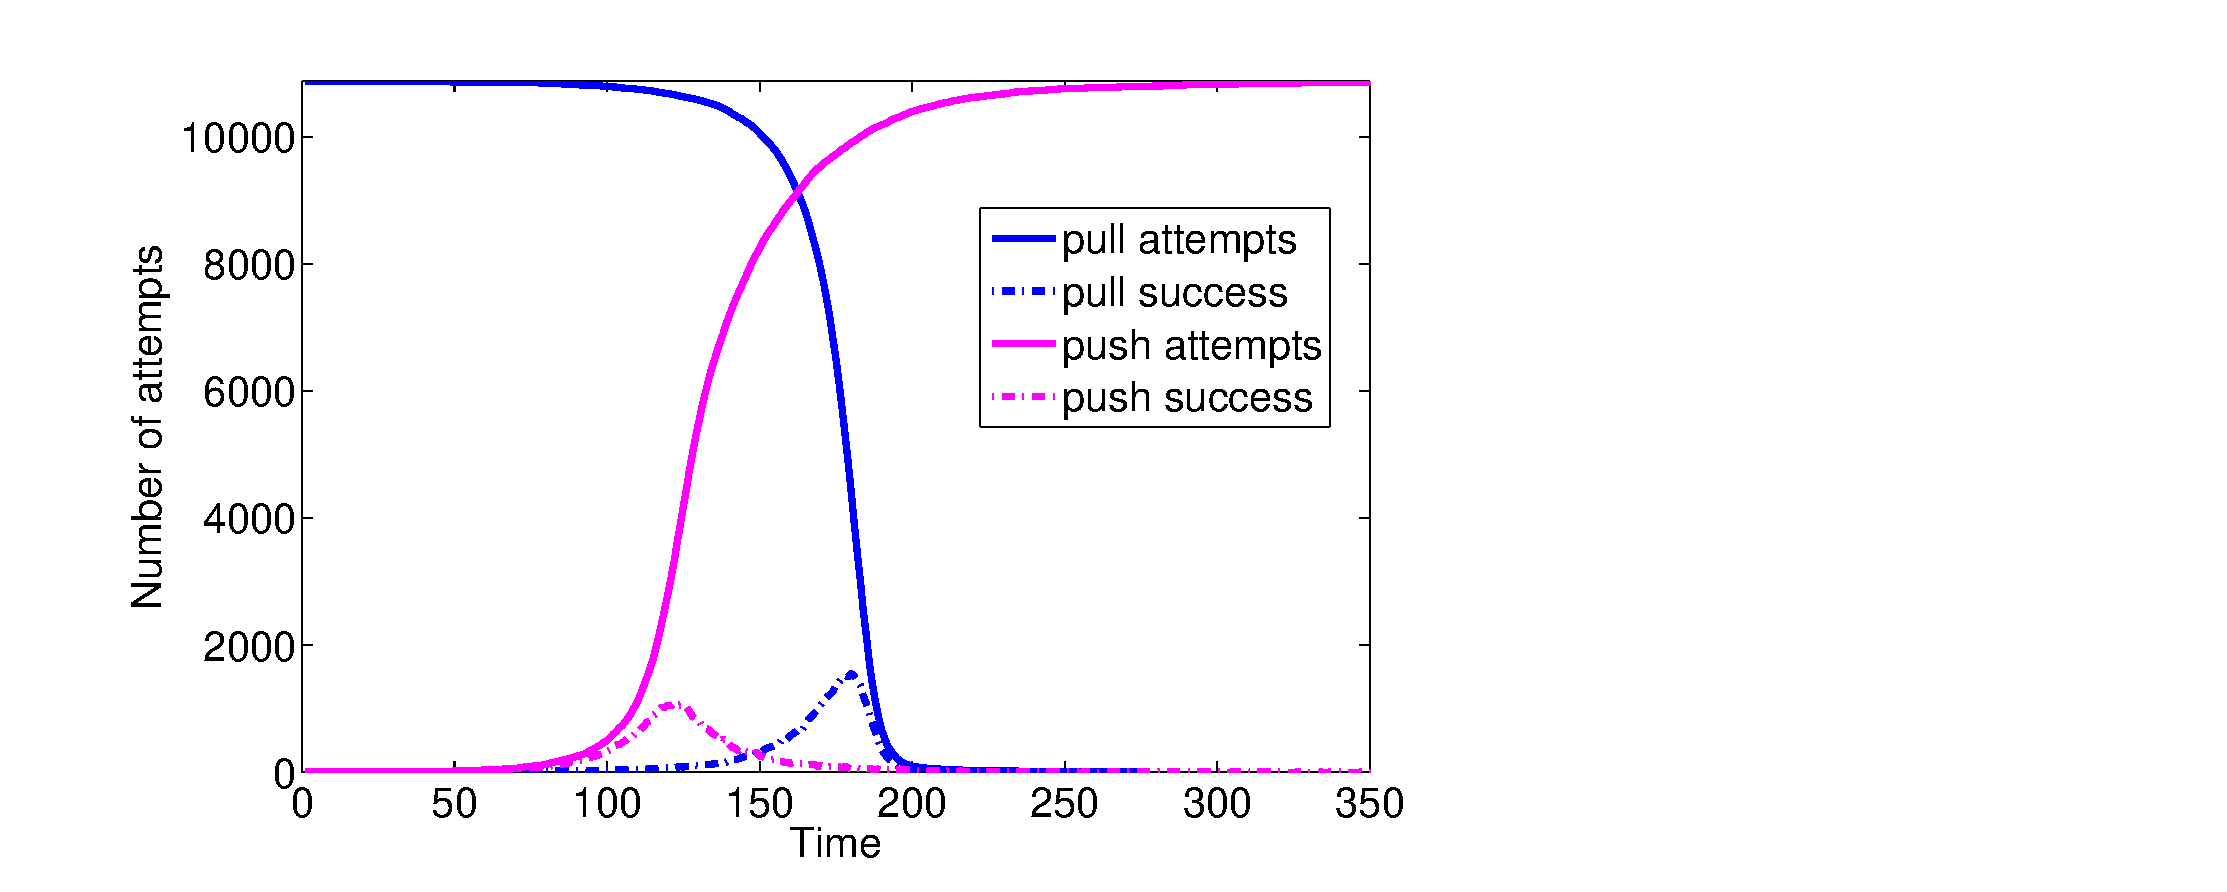
\includegraphics[scale=0.25]{./texfiles/Chapter_3/netsci/figs1/ps_pl_at_su.eps}
\caption{Pull attempts, successful pulls, push attempts, successful pushes versus time for gnutella1 network}
\label{ps_pl_at_su}
\end{figure}

\subsubsection{Strategy-x\%, automatic switch from push to pull}

In this Strategy (X-P-P), the nodes in the system follow $Blind-push$ initially and then switch to $Blind-Pull$ once x\% of the nodes in the system have 
the full message. The algorithm terminates when all the nodes in the system have the full message.

We consider the $Blind-push$ and $Blind-pull$ algorithm on a network and check how efficiently they perform over a broadcast time window. 
In figure ~\ref{ps_pl_at_su} we plot the number of attempts and the number of successful ones for the above two cases on 
  gnutella1 network (described later in this section). 
  This clearly shows pull mechanism  
  performs poorly in the beginning but picks up after a certain percentage of nodes have become senders. We observe just the opposite behavior 
  for push mechanism. Our X-P-P strategy is based on this idea to obtain the best out of both the strategies.

The X-P-P strategy cannot be implemented in a practical setting  because the nodes in the system need to maintain a global information of the percentage of nodes in the 
system having the full message which is difficult in a distributed setting like this.



\subsubsection{A distributed version of X-P-P strategy}
% To obtain a better coverage, we propose a combined strategy which combines $push$ and $pull$ in a practical way and is integrated with the give-up strategy to reduce wastage. We call this the 
% $Push Pull with giveup$ (P-P-G) technique.
% In this strategy,  each node $i$ maintains a counter ($pl\_count_i$, initialized to $0$) and an additional list $l_{i}$ which is initially empty.
% The counter counts
Here, we introduce a new strategy $Push-pull-with-giveup$ (P-P-G) which approximately mimics 
the X-P-P strategy in a distributed setting  and it functions in the following way-
Initially there  is a single node in the system which has the full message. At each time step the sender nodes in the system communicate with one of the nodes 
in their proximity and try to $push$. Among all the other non-sender nodes in the system those which have at least a single packet (i.e., nodes which have participated 
in a message transfer at least once and hence are aware of the broadcast) try to pull. Each node also keeps a local history regarding the number of unsuccessful 
communications it has participated in and once this exceeds a threshold, it `gives-up' and no longer 
participates in the broadcast. Once all the nodes have `given-up', the broadcast terminates.

% \begin{figure}
% \centering
% 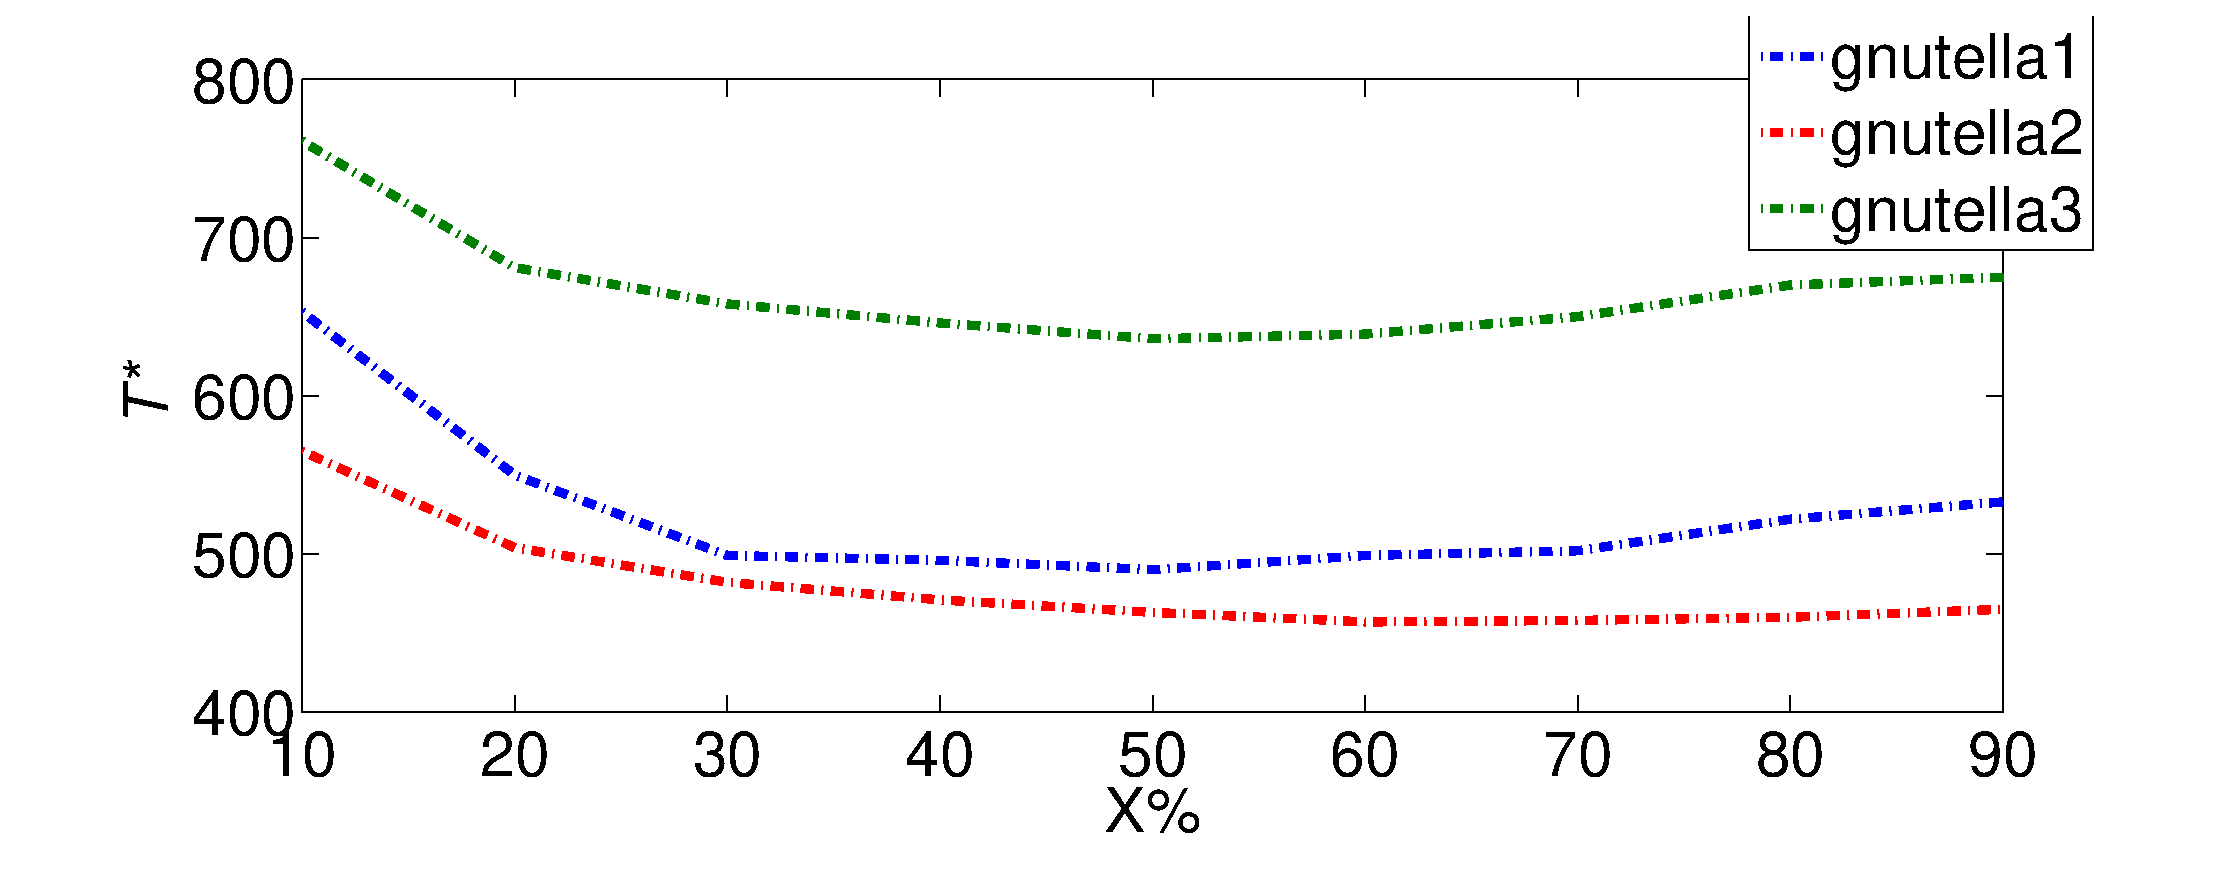
\includegraphics[scale=0.15]{figs1/xperbt.eps}
% 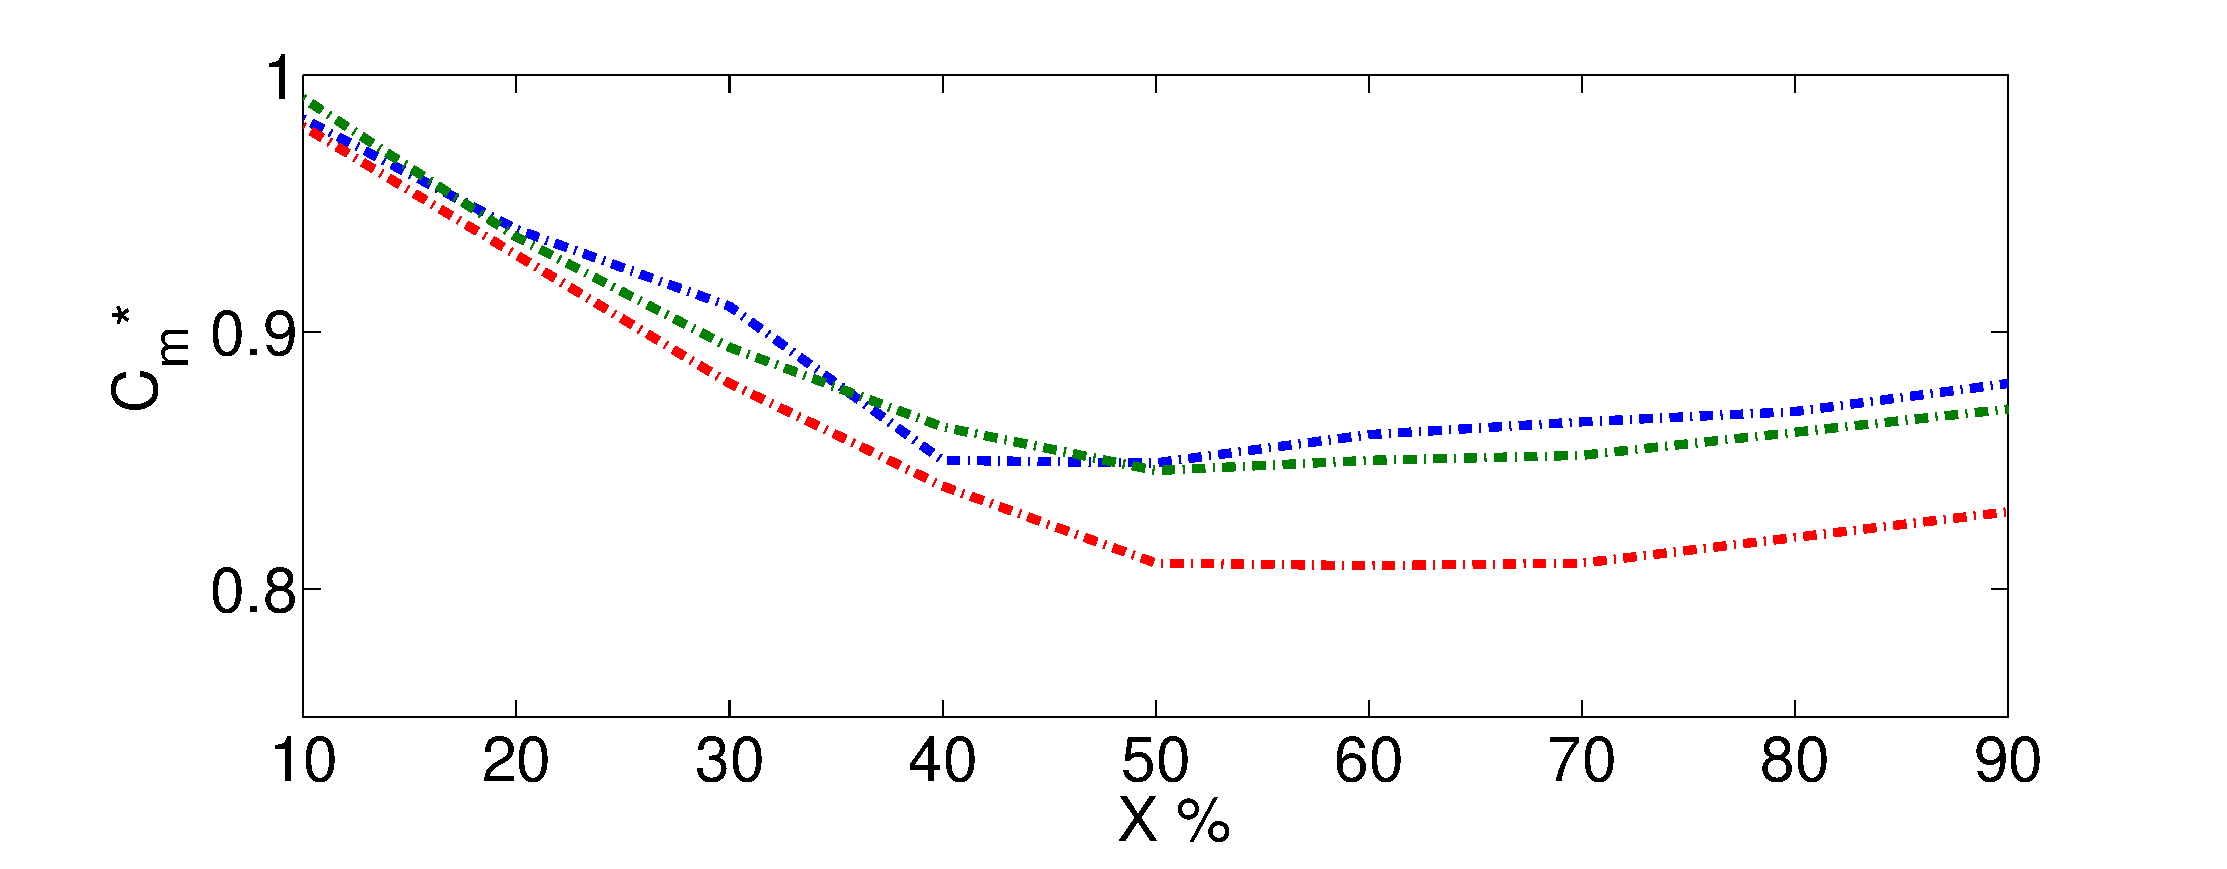
\includegraphics[scale=0.15]{figs1/xperwa.eps}
% \caption{Average broadcast time and wastage versus x for gnutella1,gnutella2 and gnutella3\vspace{-5mm}}
% \label{ps_bt}
% \end{figure}
% \medskip

\subsection{Dynamic topology}
%\vspace{-2mm}
We performed our experiments on gnutella snapshots and on synthetic topologies like complete graph, regular tree, regular graph and random graph. 
A topology specifies the potential neighborhood of a node 
- a node at each time step connects randomly to one of these nodes. A complete graph 
topology would indicate that the 
node can connect to any other node in the network while for other sparser topology it would 
connect only to a subset of them.

%\vspace{-2mm}
%\section{Theoretical analysis}
%\label{theory}
%\noindent
In this section, we first show through numerical simulations that the time to create the first sender, i.e., $T_1$, almost fully determines the overall broadcast time $T^*$. Next, we present an analytical treatment of the push technique for the minimum non-trivial case of $m=k=2$. In particular,  we attempt to compute the expected value of $T_1$ (i.e., $E(T_1)$) which is also supposed to provide an approximate estimation of $E(T^*)$. Finally, we provide pointers for the analytical treatment of the general $m=k$ case.  
We concentrate particularly on the complete graph topology; however, in a later subsection we also analytically study the message propagation for  
$m=k$ on infinite regular trees
\vspace{-3mm}
\subsection{Numerical simulations on complete graph topology}
\vspace{-1mm}



In this section, we give numeric evidence (with analytical support) that the
ratio of the overall broadcast time $T^{\ast }$ and the time to
create the first sender, i.e., $T_{1}$ converges for $n\rightarrow \infty$ to a constant which only depends on $k$. For this purpose we plot in figure~\ref%
{segSizeVsDelay_nrTrans_varyN_Mall_push_pull} the values of $Av(T^{\ast })$
and $Av(T_{1})$ respectively as we vary $n$ where $Av(x)$ represents the average of the quantity $x$ over several simulation runs. We report this distribution for
four different values of $m$ (2, 4, 8 and 16), in each case assuming that
there is only one message segment, i.e., $k=m$. Note that for B-P, the two quantities $Av(T^{\ast })$ and $Av(T_{1})$
exhibit a very similar profile irrespective of the value of $m$ chosen. In the same figure we also plot the function $n^{\frac{k-1}{k}}$ suitably scaled by a constant to show how the theoretical results which we provide in the following sections, closely approximate the numerical simulations. 

\begin{figure}[htbp] 
\centering
\includegraphics[scale=0.36]{figs1/segSizeVsDelay_nrTrans_varyN_Mall_push_pull2.eps}
\caption{$Av(T^*)$ and $Av(T_1)$ versus the number of nodes ($n$). Results are presented for (A) $m=k=2$, (B) $m=k=4$, (C) $m=k=8$, and (D) $m=k=16$. The plots also contain the suitably scaled function $n^{\frac{k-1}{k}}$ for each case.}
\label{segSizeVsDelay_nrTrans_varyN_Mall_push_pull}
\end{figure}
\vspace{-3mm}
\subsection{Performance of B-P in the limit $n\rightarrow \infty$ for complete graph topology}
\vspace{-1mm}


% We compute the expected time to obtain the first sender $E(T_{1})$ as well
% as the expected time $E\left( T^{\ast }\right) $ for broadcasting for a
% message which has $m=2$ packets ($p_{1}$ and $p_{2}$), and $s=1$ segment
% (i.e., the segment has $k=2$ packets). Recall that in push epidemic
% protocol, in each time step, a sender tries to establish a communication
% link with another agent. 
% %In each contact opportunity, only one packet can be
% %transferred from a sender to a receiver.
% As mentioned earlier, we assume only one packet can be transferred from a sender to a receiver in each contact opportunity. 
% 
% At the beginning, a source agent creates a message having 2 packets at time $%
% T_{0}$, this message has to be delivered to all other agents (i.e., $n-1$
% agents) in the network. The number of senders as a function of time is a
% step function and we denote the time of the $i^\textrm{th}$ step by $t_{i}.$ For $i$
% not too large  $\sum\limits_{j=1}^{i}t_{j}$ gives essentially the time $T_{i}$
% when the $i^\textrm{th}$ sender will be created, with the convention that $T_{0}=0$.
% Note that $\sum\limits_{i\geq 1}t_{i}$ is the broadcast time $T^{\ast }$ and 
% $t_{1}$ is the time when the first new sender is created.
% \vspace{-2mm}
% \begin{theorem}
% The random variable $\frac{t_{1}}{\sqrt{n}}$ converges as $n\rightarrow \infty $ to a
% limiting random variable $\tau _{1}$ with density $xe^{-\frac{x^{2}}{2}}$ and
% expectation $E\left( \tau _{1}\right) =\sqrt{\frac{\pi }{2}}.$ Furthermore
% for fixed $i\geq 2$ the random variable $\frac{t_{i}}{\sqrt{n}}$ converges to a
% limiting random variable $\tau _{i}$ and the following recursion holds for the
% expectations: $\frac{E\left( \tau _{i}\right) }{E\left( \tau _{i-1}\right) }%
% =\left( 1-\frac{3}{2i}\right) .$
% \end{theorem}
% \vspace{-2mm}
% \begin{theorem}
% $\frac{T^{\ast }}{\sqrt{n}}$ converges to a limiting random variable $s^{\ast }$ with $%
% E\left( s^{\ast }\right) =\sum\limits_{i=1}^{\infty }E\left( \tau
% _{i}\right) =2\cdot \sqrt{\frac{\pi }{2}}$
% \end{theorem}
% \vspace{-3mm}
% \begin{proof}
% (sketch). We will sketch in the following some of the important steps in the
% proof. For the probability that the first new sender is created at time $t$
% we have%
% \[
% \Pr \left\{ t_{1}=t\right\} =\frac{t-1}{n}\prod\limits_{l=1}^{t-2}\left( 1-%
% \frac{l}{n}\right) ,t\geq 2
% \]%
% Writing $\left( 1-\frac{l}{n}\right) =e^{-\frac{l}{n}+O\left( \frac{l^{2}}{%
% n^{2}}\right) }$we have for the cumulative distribution function 
% \begin{eqnarray*}
% \Pr \left\{ \frac{t_{1}}{\sqrt{n}}\leq x\right\}  &=&\sum\limits_{t\leq x%
% \sqrt{n}}\frac{t-1}{n}\prod\limits_{l=1}^{t-2}\left( 1-\frac{l}{n}\right)  \\
% &=&\sum\limits_{t\leq x\sqrt{n}}\frac{t}{n}e^{-\frac{t^{2}}{2n}+O\left( 
% \frac{t^{3}}{n^{2}}\right) }
% \end{eqnarray*}%
% For $n\rightarrow \infty $, the sum in the last expression converges to $%
% \int\limits_{0}^{x}ye^{-\frac{y^{2}}{2}}dy.$  Hence the limiting density is
% given by $ye^{-\frac{y^{2}}{2}}$ and the expectation by $\int\limits_{0}^{%
% \infty }y^{2}e^{-\frac{y^{2}}{2}}dy=\sqrt{\frac{\pi }{2}}.$ In a similar
% fashion one can obtain the conditional limiting distribution of $\tau _{i}$
% given the value of $b_{i-1}:=\sum\limits_{m=1}^{i-1}m\tau _{m}:$ 
% \[
% \Pr \left\{ \tau _{i}\leq x\right\} =\int\limits_{0}^{x}i\left(
% b_{i-1}+i\tau _{i}\right) e^{-i\left( \tau _{i}b_{i-1}+k\tau
% _{i}^{2}/2\right) }d\tau _{i}
% \]%
% Note that $b_{i}\sqrt{n}$ is the approximate number of nodes with one
% packet up to time $T_{i}.$ By a straightforward but lengthy computation
% using the previous expression for the conditional distribution of $\tau _{i}$
% it can be shown that the recursion $\frac{E\left( \tau _{i}\right) }{E\left(
% \tau _{i-1}\right) }=\left( 1-\frac{3}{2i}\right) $ holds. We will derive
% from this recursion now the expression for $s^{\ast }.$ Clearly we have 
% \[
% E\left( \tau _{i}\right) =\prod\limits_{j\geq 2}^{i}\frac{2j-3}{2j}E\left(
% \tau _{1}\right) 
% \]%
% and hence $s^{\ast }=\left( 1+\sum\limits_{i\geq 2}\prod\limits_{j\geq 2}^{i}%
% \frac{2j-3}{2j}\right) E\left( \tau _{1}\right) .$ Rewriting the product as%
% \[
% \prod\limits_{j\geq 2}^{i}\frac{2j-3}{2j}=\frac{\left( 2\left( i-1\right)
% \right) !}{4^{i-1}\left( \left( i-1\right) !\right) ^{2}i}
% \]%
% we have%
% \[
% s^{\ast }=\left( \sum\limits_{i=0}\frac{\left( 2i\right) !\cdot 2}{%
% 4^{i-1}\left( i!\right) ^{2}\cdot 2\left( i+1\right) }\right) E\left( \tau
% _{1}\right) 
% \]%
% The function 
% \[
% g\left( z\right) :=\sum\limits_{i=0}\frac{\left( 2i\right) !}{%
% 4^{i-1}\left( i!\right) ^{2}\cdot 2\left( i+1\right) }z^{2\left( i+1\right) }
% \]%
% converges for $\left\vert z\right\vert \leq 1$ and satisfies%
% \[
% \frac{d}{dz}g\left( z\right) =z\cdot \frac{d}{dz}\arcsin z=z\cdot \frac{1}{%
% \sqrt{1-z^{2}}}
% \]%
% as can be easily seen by comparing with the Taylor expansion of the right hand side. Hence 
% \[
% g\left( 1\right) =\int\limits_{0}^{1}\frac{z}{\sqrt{1-z^{2}}}dz=1
% \]%
% and $s^{\ast }=2E\left( \tau _{1}\right).$
% \end{proof}
% 
% It is important to note that the above computations can be carried out essentially up to a time $t$ where there are $\sqrt{n}$ senders. The remaining growth is very fast - actually of logarithmic order since several new senders in every time step get produced.
% \vspace{-3mm}
We compute the expected time to obtain the first sender $E(T_{1})$ as well
as the expected time $E\left( T^{\ast }\right) $ for broadcasting for a
message which has $m=2$ packets ($p_{1}$ and $p_{2}$), and $s=1$ segment
(i.e., the segment has $k=2$ packets). Recall that in push epidemic
protocol, in each time step, a sender tries to establish a communication
link with another agent. 
%In each contact opportunity, only one packet can be
%transferred from a sender to a receiver.
As mentioned earlier, we assume only one packet can be transferred from a
sender to a receiver in each contact opportunity.

At the beginning, a source agent creates a message having 2 packets at time $%
T_{0}$, this message has to be delivered to all other agents (i.e., $n-1$
agents) in the network. The number of senders as a function of time is a
step function and we denote the time of the $i^\textrm{th}$ step by $t_{i}.$
For $i$ not too large $\sum\limits_{j=1}^{i}t_{j}$ gives essentially the
time $T_{i}$ when the $i^\textrm{th}$ sender will be created, with the
convention that $T_{0}=0$. Note that $\sum\limits_{i\geq 1}t_{i}$ is the
broadcast time $T^{\ast }$ and $t_{1}$ is the time when the first new sender
is created. \vspace{-2mm} 
\begin{theorem}
The random variable $\frac{t_{1}}{\sqrt{n}}$ converges as $n\rightarrow \infty $ to a
limiting random variable $\tau _{1}$ with density $xe^{-\frac{x^{2}}{2}}$ and
expectation $E\left( \tau _{1}\right) =\sqrt{\frac{\pi }{2}}.$ Furthermore
for fixed $i\geq 2$ the random variable $\frac{t_{i}}{\sqrt{n}}$ converges to a
limiting random variable $\tau _{i}$ and the following recursion holds for the
expectations: $\frac{E\left( \tau _{i}\right) }{E\left( \tau _{i-1}\right) }%
=\left( 1-\frac{3}{2i}\right) .$
\end{theorem}
\vspace{-2mm} 
\begin{theorem}
$\frac{T^{\ast }}{\sqrt{n}}$ converges to a limiting random variable $s^{\ast }$ with $%
E\left( s^{\ast }\right) =\sum\limits_{i=1}^{\infty }E\left( \tau
_{i}\right) =2\cdot \sqrt{\frac{\pi }{2}}$
\end{theorem}
\vspace{-3mm} 
\begin{proof}
(sketch). We will sketch in the following some of the important steps in the
proof. For the probability that the first new sender is created at time $t$
we have%
\[
\Pr \left\{ t_{1}=t\right\} =\frac{t-1}{n}\prod\limits_{l=1}^{t-2}\left( 1-%
\frac{l}{n}\right) ,t\geq 2
\]%
Writing $\left( 1-\frac{l}{n}\right) =e^{-\frac{l}{n}+O\left( \frac{l^{2}}{%
n^{2}}\right) }$we have for the cumulative distribution function 
\begin{eqnarray*}
\Pr \left\{ \frac{t_{1}}{\sqrt{n}}\leq x\right\}  &=&\sum\limits_{t\leq x%
\sqrt{n}}\frac{t-1}{n}\prod\limits_{l=1}^{t-2}\left( 1-\frac{l}{n}\right)  \\
&=&\sum\limits_{t\leq x\sqrt{n}}\frac{t}{n}e^{-\frac{t^{2}}{2n}+O\left( 
\frac{t^{3}}{n^{2}}\right) }
\end{eqnarray*}%
For $n\rightarrow \infty $, the sum in the last expression converges to $%
\int\limits_{0}^{x}ye^{-\frac{y^{2}}{2}}dy.$  Hence the limiting density is
given by $ye^{-\frac{y^{2}}{2}}$ and the expectation by $\int\limits_{0}^{%
\infty }y^{2}e^{-\frac{y^{2}}{2}}dy=\sqrt{\frac{\pi }{2}}.$ In a similar
fashion one can obtain the conditional limiting distribution of $\tau _{i}$
given the value of $b_{i-1}:=\sum\limits_{m=1}^{i-1}m\tau _{m}:$ 
\[
\Pr \left\{ \tau _{i}\leq x\right\} =\int\limits_{0}^{x}i\left(
b_{i-1}+i\tau _{i}\right) e^{-i\left( \tau _{i}b_{i-1}+k\tau
_{i}^{2}/2\right) }d\tau _{i}
\]%
Note that $b_{i}\sqrt{n}$ is the approximate number of nodes with one
packet up to time $T_{i}.$ By a straightforward but lengthy computation
using the previous expression for the conditional distribution of $\tau _{i}$
it can be shown that the recursion $\frac{E\left( \tau _{i}\right) }{E\left(
\tau _{i-1}\right) }=\left( 1-\frac{3}{2i}\right) $ holds. We will derive
from this recursion now the expression for $s^{\ast }.$ Clearly we have 
\[
E\left( \tau _{i}\right) =\prod\limits_{j\geq 2}^{i}\frac{2j-3}{2j}E\left(
\tau _{1}\right) 
\]%
and hence $s^{\ast }=\left( 1+\sum\limits_{i\geq 2}\prod\limits_{j\geq 2}^{i}%
\frac{2j-3}{2j}\right) E\left( \tau _{1}\right) .$ Rewriting the product as%
\[
\prod\limits_{j\geq 2}^{i}\frac{2j-3}{2j}=\frac{\left( 2\left( i-1\right)
\right) !}{4^{i-1}\left( \left( i-1\right) !\right) ^{2}i}
\]%
we have%
\[
s^{\ast }=\left( \sum\limits_{i=0}\frac{\left( 2i\right) !\cdot 2}{%
4^{i-1}\left( i!\right) ^{2}\cdot 2\left( i+1\right) }\right) E\left( \tau
_{1}\right) 
\]%
The function 
\[
g\left( z\right) :=\sum\limits_{i=0}\frac{\left( 2i\right) !}{%
4^{i-1}\left( i!\right) ^{2}\cdot 2\left( i+1\right) }z^{2\left( i+1\right) }
\]%
converges for $\left\vert z\right\vert \leq 1$ and satisfies%
\[
\frac{d}{dz}g\left( z\right) =z\cdot \frac{d}{dz}\arcsin z=z\cdot \frac{1}{%
\sqrt{1-z^{2}}}
\]%
as can be easily seen by comparing with the Taylor expansion of the right hand side. Hence 
\[
g\left( 1\right) =\int\limits_{0}^{1}\frac{z}{\sqrt{1-z^{2}}}dz=1
\]%
and $s^{\ast }=2E\left( \tau _{1}\right).$
\end{proof}

It is important to note that the above computations can be carried out
essentially up to a time $t$ where there are $\sqrt{n}$ senders. The
remaining growth is very fast - actually of logarithmic order since several
new senders in every time step get produced. \vspace{-2mm}
\subsection{A short indication of the results for the general case $m=k$}
\vspace{-1mm}
% Here we present a sketch of the approach to general $m=k$ case. We are
% interested in the waiting time $t_{1}$ for the appearance of the first
% sender. For that, one has to understand how the number of sites which have
% exactly say $l$ packets grows with $t.$ 
% 
% (i) 1-packet carriers grow essentially as $t$ (because the initial sender
% node establishes contacts in most cases, a new node from the pool $n$),
% 
% (ii) 2-packet carriers grow essentially as $\sum\limits^{t}\frac{i}{n}\sim \frac{%
% t^{2}}{2n}$ since at time $i$ the probability to establish contact again from the $i$
% 1-packet carriers is $\frac{i}{n}.$~\footnote{This sum and all the
% following are random variables but for $t$ large enough one can use the
% central limit theorem -- furthermore the fluctuations are small compared to
% the leading term -- can all be worked out nicely and we plan to report this in a forthcoming paper.}
% 
% (iii) 3-packet carriers grow essentially as $\sum\limits^{t}\frac{1}{n}\frac{i^{2}%
% }{2n}\sim \frac{t^{3}}{3\cdot 2\cdot n^{2}}$,
% 
% \bigskip 
% 
% (iv) and finally the $(m-1)$-packet carriers grow essentially as $\frac{t^{m-1}}{\left(
% m-1\right) !n^{m-2}}$
% 
% With this estimation we can now proceed as in the $m=2$ case (conceptually of
% course) since%
% \begin{eqnarray*}
% \Pr \left( t_{1}=t\right)  &\sim &\frac{t^{m-1}}{\left( m-1\right) !n^{m-1}}%
% \prod\limits_{i}^{t}\left( 1-\frac{i^{m-1}}{\left( m-1\right) !n^{m-1}}%
% \right)  \\
% &\sim &\frac{t^{m-1}}{\left( m-1\right) !n^{m-1}}e^{-\frac{t^{m}}{m!n^{m-1}}}
% \end{eqnarray*}%
% From this one sees that $t_{1}$ is of the order $n^{\frac{m-1}{m}}$ .
% 
% More precisely one has for the limiting quantity $\tau
% _{1}=\lim_{n\rightarrow \infty }\frac{t_{1}}{n^{\frac{m-1}{m}}}:$%
% \[
% E\left( \tau _{1}\right) =\int\limits_{0}^{\infty }\frac{y^{m}}{\left(
% m-1\right) !}e^{-\frac{y^{m}}{m!}}dy
% \]%
% and $\tau _{1}$ has density $\frac{y^{m-1}}{\left( m-1\right) !}e^{-\frac{%
% y^{m}}{m!}}.$
Here we present a sketch of the approach to general $m=k$ case. We are
interested in the waiting time $t_{1}$ for the appearance of the first
sender. For that one has to understand how the number of sites which have
exactly say $l$ packets grows with $t.$

(i) 1-packet carriers grow essentially as $t$ (because the initial sender
node establishes contacts in most cases a new node from the pool $n$),

(ii) 2-packet carriers grow essentially as $\sum\limits^{t}\frac{i}{n}\sim 
\frac{t^{2}}{2n}$ since at time $i$ the probability to establish contact
again from the $i$ 1-packet carriers is $\frac{i}{n}.$~\footnote{%
This sum and all the following are random variables but for $t$ large enough
one can use the central limit theorem -- furthermore the fluctuations are
small compared to the leading term -- can all be worked out nicely and we
plan to report this in a forthcoming paper.}

(iii) 3-packet carriers grow essentially as $\sum\limits^{t}\frac{1}{n}\frac{%
i^{2}}{2n}\sim \frac{t^{3}}{3\cdot 2\cdot n^{2}}$,

\bigskip

(iv) and finally the $(m-1)$-packet carriers grow essentially as $\frac{%
t^{m-1}}{\left( m-1\right) !n^{m-2}}$

With this estimation we can now proceed as in the $m=2$ case (conceptually
of course) since%
\begin{eqnarray*}
\Pr \left( t_{1}=t\right) &\sim &\frac{t^{m-1}}{\left( m-1\right) !n^{m-1}}%
\prod\limits_{i}^{t}\left( 1-\frac{i^{m-1}}{\left( m-1\right) !n^{m-1}}%
\right) \\
&\sim &\frac{t^{m-1}}{\left( m-1\right) !n^{m-1}}e^{-\frac{t^{m}}{m!n^{m-1}}}
\end{eqnarray*}%
From this one sees that $t_{1}$ is of the order $n^{\frac{m-1}{m}}$ .

More precisely one has for the limiting quantity $\tau
_{1}=\lim_{n\rightarrow \infty }\frac{t_{1}}{n^{\frac{m-1}{m}}}:$%
\[
E\left( \tau _{1}\right) =\int\limits_{0}^{\infty }\frac{y^{m}}{\left(
m-1\right) !}e^{-\frac{y^{m}}{m!}}dy 
\]%
and $\tau _{1}$ has density $\frac{y^{m-1}}{\left( m-1\right) !}e^{-\frac{%
y^{m}}{m!}}.$

\subsection{Theoretical analysis for infinite regular trees}   
In this section we study the characteristics of message propagation with $m=k$ on
infinite regular trees. The same analysis provided here holds mutatis
mutandis for trees generated by branching processes with Poisson offspring
distribution.

We start with the case of $d$ $-$ regular trees for $d\geq 3$ with a
distinguished root index $0$ which acts as the initial sender. For
simplicity we give the root an out-degree of $d-1$ by attaching a virtual
``mother vertex'' to the root which is also a sender but has only one
offspring and is not counted in the estimation of sender nodes (this helps us avoid
handling the initial steps (when only the root is having the message)
differently from the later steps). Let $A_{l}\left( t\right) ,$ $0\leq l<m,$
be the number of nodes on the tree which have exactly $l$ packets at time $t
$ and have a direct communication link to one of the sender nodes at time $t$. Note that each of the so defined nodes has exactly one connection to a
sender node due to the tree structure and the initial condition of having
just one sender at the beginning. We get the following linear exact
recursion for the expectation $a_{l}\left( t+1\right) :=\mathbb{E}\left(
A_{l}\left( t+1\right) \right) $ at time $t+1:$%
\begin{eqnarray*}
a_{l}\left( t+1\right)  &=&\frac{k-1}{k}a_{l}\left( t\right) +\frac{1}{k}%
a_{l-1}\left( t\right) ,1\leq l\leq m-1 \\
a_{0}\left( t+1\right)  &=&\frac{k-1}{k}a_{m-1}\left( t\right) +\frac{k-1}{k}%
a_{0}\left( t\right) 
\end{eqnarray*}%
Note that for the expected number of sender nodes $s_{t}$ at time $t$ we
have 
\[
s_{t}=\sum\limits_{t^{\prime }<t}\frac{1}{k}a_{m-1}\left( t^{\prime }\right) 
\]
The asymptotic rate of growth of the variables $\left\{ a_{i}\left( t\right)
\right\} $ as well as $s_{t}$ is entirely determined by the value of the
largest eigenvalue of the associated transition matrix. The maximal
eigenvalue of the associated characteristic polynomial is given by 
\[
\lambda _{\max }=\frac{k-1}{k}+\left( \frac{k-1}{k}\left( \frac{1}{k}\right)
^{m-1}\right) ^{\frac{1}{m}}=\frac{k-1+\left( k-1\right) ^{1/m}}{k}
\]%
We study the maximum of the function $\frac{x-1+\left( x-1\right) ^{1/m}}{x}$
for $x>2.$ Setting the derivative to zero gives the condition 
\[
\left( x-1\right) ^{m-1}=\left( \frac{m-1}{m}x-1\right) ^{m},x>2
\]%
We therefore get
\[
\left( 1-\frac{x}{m\left( x-1\right) }\right) ^{m-1}\cdot \left( x-1-\frac{%
x}{m}\right)=1 
\]%
and in the limit $m\rightarrow \infty $ we obtain%
\[
\left( x-1\right) e^{-\frac{x}{x-1}}=1
\]%
Note that the whole computation holds also for the case of a Poisson
offspring distribution with expectation $k-1.$
\medskip
\section{Experiment on different network topologies}
\label{suggestions}
%\vspace{-1mm}
\noindent
In this section we systematically study the effect of topology of the underlying contact network on the broadcast time and wastage and come up with some suggestions which we 
feel will be helpful while designing networks.  
%First we analyze the B-P algorithm on complete graph topology and observe that the broadcast time scales 
%as $n^{\frac{k-1}{k}}$. 
We first analyze B-P algorithm on different topologies like regular graph, regular tree and random graph. In particular, we wish to 
check whether the average degree ($d$) of the underlying contact network influences the 
 performance metrics. 
 %Since it is difficult to interpolate through every value of $d$ for a real network, we perform our simulations on the synthetic networks.
 In the later part of this section we make a comparative study of different broadcast strategies (discussed in section ~\ref{algorithm_outline}) and also
 reinspect into their sparser variants to identify the effect of lowering the value of $d$ 
 through removal of edges without hampering network connectivity.
\subsection{Blind push on different topologies} 
\if{0}
%\vspace{-5mm}
\subsection{Blind push on complete graph}
% \vspace{-2mm}
 We analyze the performance of B-P on complete graph topology. A complete graph topology indicates that a node in the system can communicate with any other node. 
 We provide numeric evidence (with analytical support) that the
ratio of the overall broadcast time $T^{\ast }$ and the time to
create the first sender, i.e., $T_{1}$ converges to a constant which only depends on $k$. 
For this purpose we plot in figure~\ref%
{segSizeVsDelay_nrTrans_varyN_Mall_push_pull} the values of $Av(T^{\ast })$
and $Av(T_{1})$ respectively as we vary $n$ where $Av(y)$ represents the average of the quantity $y$ over several simulation runs. We report this distribution for
four different values of $m$ (2, 4, 8 and 16), in each case assuming that
there is only one message segment, i.e., $k=m$. Note that for B-P, the two quantities $Av(T^{\ast })$ and $Av(T_{1})$
exhibit a very similar profile irrespective of the value of $m$ chosen. In the same figure we also plot the function $n^{\frac{k-1}{k}}$ suitably scaled by a constant to show how the theoretical results which we provide next, closely approximate the numerical simulations. 

\begin{figure}[htbp] 
\centering
\includegraphics[scale=0.36]{./texfiles/Chapter_3/netsci/figs1/segSizeVsDelay_nrTrans_varyN_Mall_push_pull2.eps}
\caption{$Av(T^*)$ and $Av(T_1)$ versus the number of nodes ($n$). Results are presented for (A) $m=k=2$, (B) $m=k=4$, (C) $m=k=8$, and (D) $m=k=16$. The plots also contain the suitably scaled function $n^{\frac{k-1}{k}}$ for each case.}
\label{segSizeVsDelay_nrTrans_varyN_Mall_push_pull}
\end{figure}
%\subsection{Performance of B-P in the limit $n\rightarrow \infty$ for complete graph topology}
\subsubsection{Analytical estimate}

We initially start by considering a message which has $m=2$ packets and $s=1$ segment (i.e., the segment has $k=2$ packets). We compute the expected time to 
obtain the first sender\footnote{
Note that first sender refers to the first node (other than the initiator) which 
receives the full message during the broadcast phase.
} $E(T_1)$. 
%and the expected time for broadcast $E(T^{\ast})$. 
It is important to note that $T_1$ is an indicator for the total broadcast time $T^*$ since the remaining growth is of logarithmic order as after creation of the first sender, 
several senders are produced at regular interval thus speeding
up the transfer exponentially. 
We provide an outline of the analytical expression, the detail is more involved and is ommitted in the interest of space. 
 
At time $T_0$, an initiator is created and it has the full message. Since we are considering 
message size of $2$ so the first sender can be created at least in 2 time steps which is possible
 if the same node is selected in these two time steps. Next we calculate 
$Pr\{T_1=t\}$ that is the probability that the  first sender is created at time $t$. This implies
for the $t-1$ time steps, only the nodes without any packets are selected and at time step $t$ one 
from the $t-1$ nodes are selected. So we have


\begin{align*}
\Pr \{ T_{1}=t\} &=(1-\frac{1}{n})(1-\frac{2}{n})(1-\frac{3}{n})...(1-\frac{t-2}{n})(\frac{t-1}{n}) \\ 
 &=\frac{t-1}{n}\prod\limits_{l=1}^{t-2}( 1-%
\frac{l}{n}) ,t\geq 2
\end{align*}
Infact if $\tau_i$ represent the time to create the first sender then it can be shown that the recursion  $\frac{E\left( \tau _{i}\right) }{E\left(
\tau _{i-1}\right) }=\left( 1-\frac{3}{2i}\right) $ holds. 
From this one can show that $E(T^*)=2*E(T_1)$
\if{0}
Writing $\left( 1-\frac{l}{n}\right) =e^{-\frac{l}{n}+O\left( \frac{l^{2}}{%
n^{2}}\right) }$we have for the cumulative distribution function 
\begin{eqnarray*}
\Pr \left\{ \frac{t_{1}}{\sqrt{n}}\leq x\right\}  &=&\sum\limits_{t\leq x%
\sqrt{n}}\frac{t-1}{n}\prod\limits_{l=1}^{t-2}\left( 1-\frac{l}{n}\right)  \\
&=&\sum\limits_{t\leq x\sqrt{n}}\frac{t}{n}e^{-\frac{t^{2}}{2n}+O\left( 
\frac{t^{3}}{n^{2}}\right) }
\end{eqnarray*}%
For $n\rightarrow \infty $, the sum in the last expression converges to $%
\int\limits_{0}^{x}ye^{-\frac{y^{2}}{2}}dy.$  Hence the limiting density is
given by $ye^{-\frac{y^{2}}{2}}$ and the expectation by $\int\limits_{0}^{%
\infty }y^{2}e^{-\frac{y^{2}}{2}}dy=\sqrt{\frac{\pi }{2}}.$
%\vspace{-2mm}
\fi

Generalizing for case where $k$ $>$ 2, we calculate the time to create the first sender $T_1$. To do it we look into how the number of nodes with exactly $l$ packets (say)
grow with $t$ ($l$ varies from $1$ to $k$ -1). 
We can show that the number of nodes with $l$ packets 
 grow  as $\frac{%
t^{l}}{\left( l\right) !n^{l-1}}$

With this estimation we can now proceed in the same way as we did in case of $k=2$ case and show that 
\begin{eqnarray*}
\Pr \left( T_{1}=t\right) &\sim &\frac{t^{k-1}}{\left( k-1\right) !n^{k-1}}%
\prod\limits_{i}^{t}\left( 1-\frac{i^{k-1}}{\left( k-1\right) !n^{k-1}}%
\right) \\
&\sim &\frac{t^{k-1}}{\left( k-1\right) !n^{k-1}}e^{-\frac{t^{k}}{k!n^{k-1}}}
\end{eqnarray*}%

From the above probability distribution of $T_{1}$ we calculate $E(T_{1})=\sum t*\frac{t^{k-1}}{\left( k-1\right) !n^{k-1}}e^{-\frac{t^{k}}{k!n^{k-1}}}$
and through a lengthy calculation can show that $E(T_{1})$ is of the order $n^{\frac{k-1}{k}}$.
 
%  It is important to note that $T_1$ is an indication for the total broadcast time $T^*$ since the remaining growth is very fast - actually of 
%  logarithmic order since several senders at every time step get produced.
 \vspace{-2mm}
 \fi
%\subsection{Blind push on sparser topologies}
%\vspace{-2mm}
The results of B-P on complete graph are similar to the ones provided in section \ref{res_complete}, hence we concentrate on the sparser topologies. 
In specific, we empirically analyze the B-P algorithm on regular-tree, regular-graph and random-graph. For each topology we consider $n=200$, $m = 4$ and $k=2$.
Note that here we consider that the message has $2$ segments and each segment has $k=2$ packets. 
We then vary the average degree $d$ for each of these networks and check how broadcast delay and wastage depend on it. Remarkably, for each of these topologies 
- regular tree (figure ~\ref{DiffTopologyTree_N200_varyD_push_pull}), regular graph (figure ~\ref{DiffTopologyGraph_N200_varyD_push_pull}) and random graph 
(figure ~\ref{DiffTopologyGnp_N200_varyD_push_pull}), one can observe that there is a critical value of $d$ for which we obtain minimum broadcast delay and 
wastage.
% Here, we assume a finite regular tree topology for $G$ where $n = 200$, $m = 4$ and $k=2$. We vary the degree $d$ of the tree from values ranging from 2 to 10 (see figure~\ref{DiffTopologyTree_N200_varyD_push_pull}). An important observation is that both the broadcast time and the broadcast wastage become significantly low at a critical value of $d$. In fact, for this value of $d$, the metrics of interest reach their minima for B-P technique. 
% \vspace{-3mm}
% \subsection{Regular graph}
% 
% Here, we assume a regular graph topology for $G$ where $n = 200$, $m = 4$ and $k=2$. Once again, we vary the degree $d$ of the graph from values ranging from 1 to 200 (see figure~\ref{DiffTopologyGraph_N200_varyD_push_pull}). The same observation that both the broadcast time and the broadcast wastage become significantly low for a certain value of $d$ also hold in this case and for this value of $d$ the broadcast time is found to scale as $\log{(n)}$. Again at this value of $d$, the metrics of interest reach their minima for the B-P technique.  
% 
% % \begin{figure}
% % \centering
% % 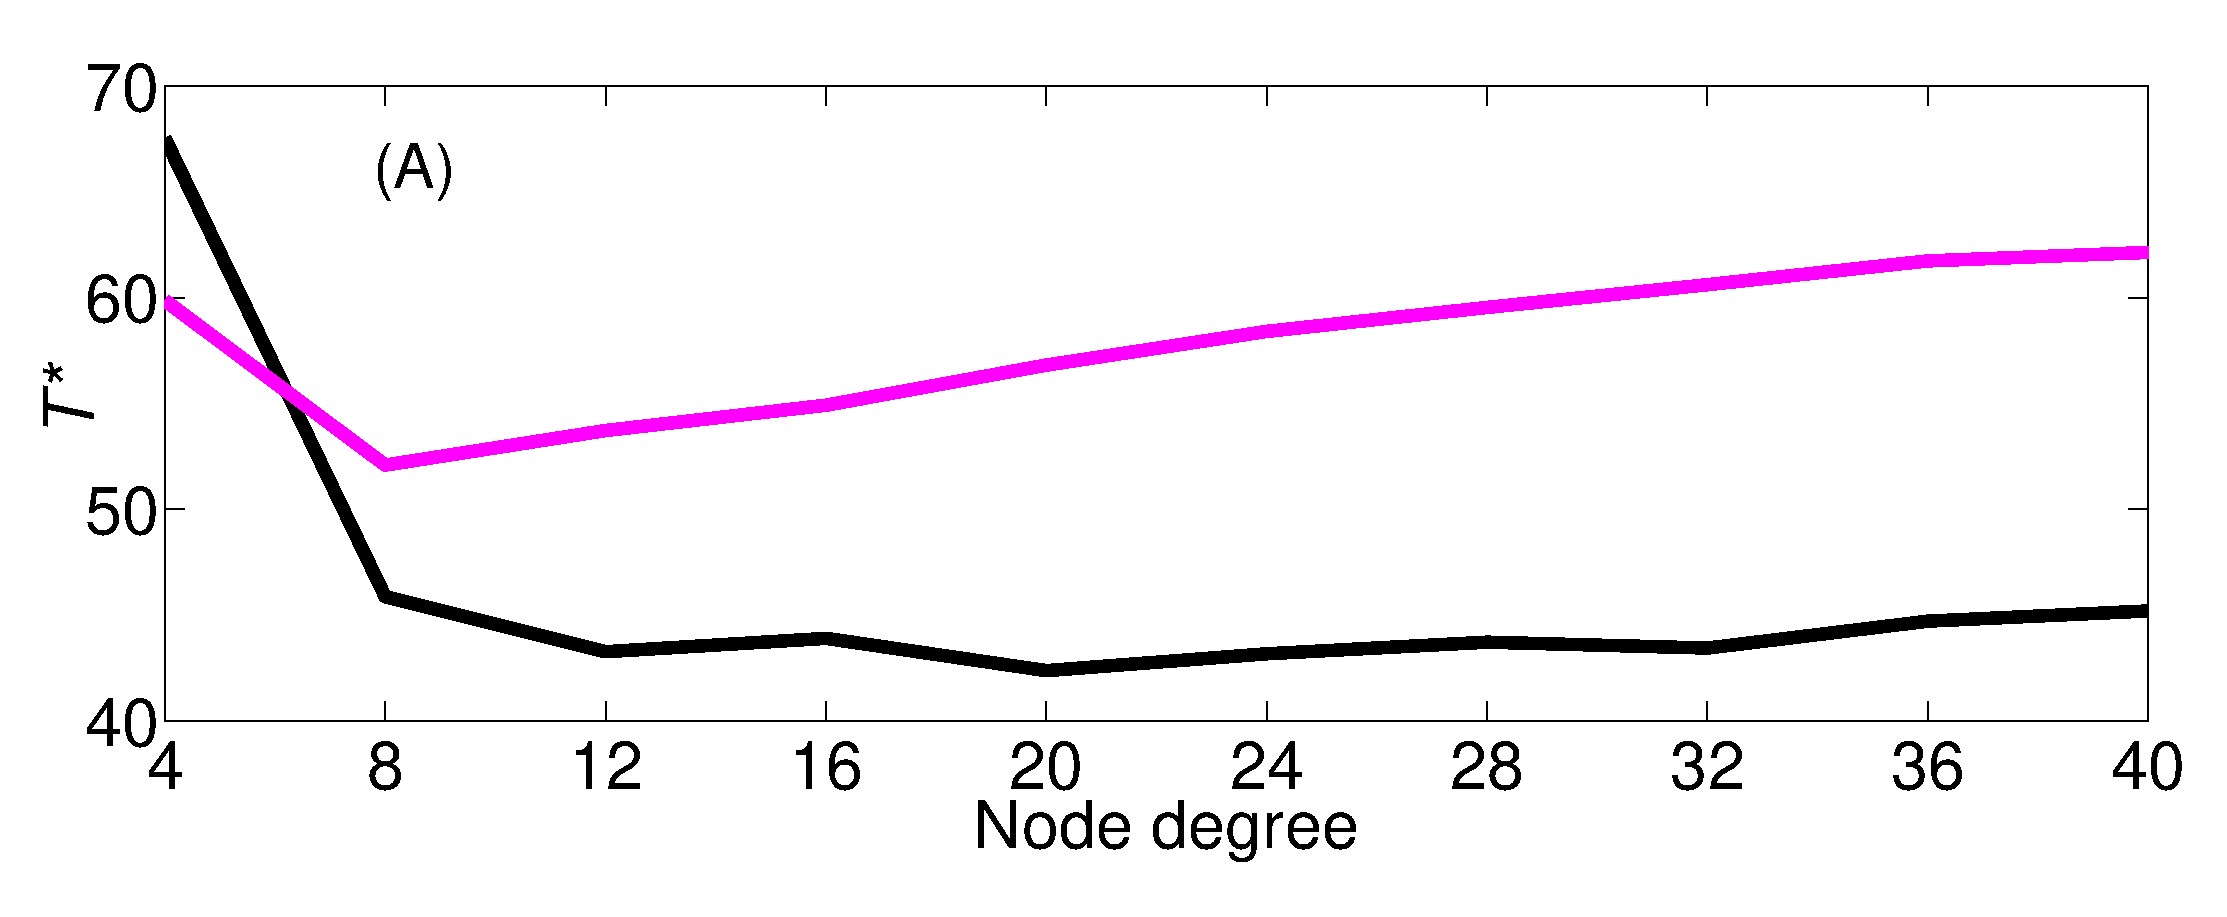
\includegraphics[scale=0.15]{figs1/random_graphs_delay.eps}
% % 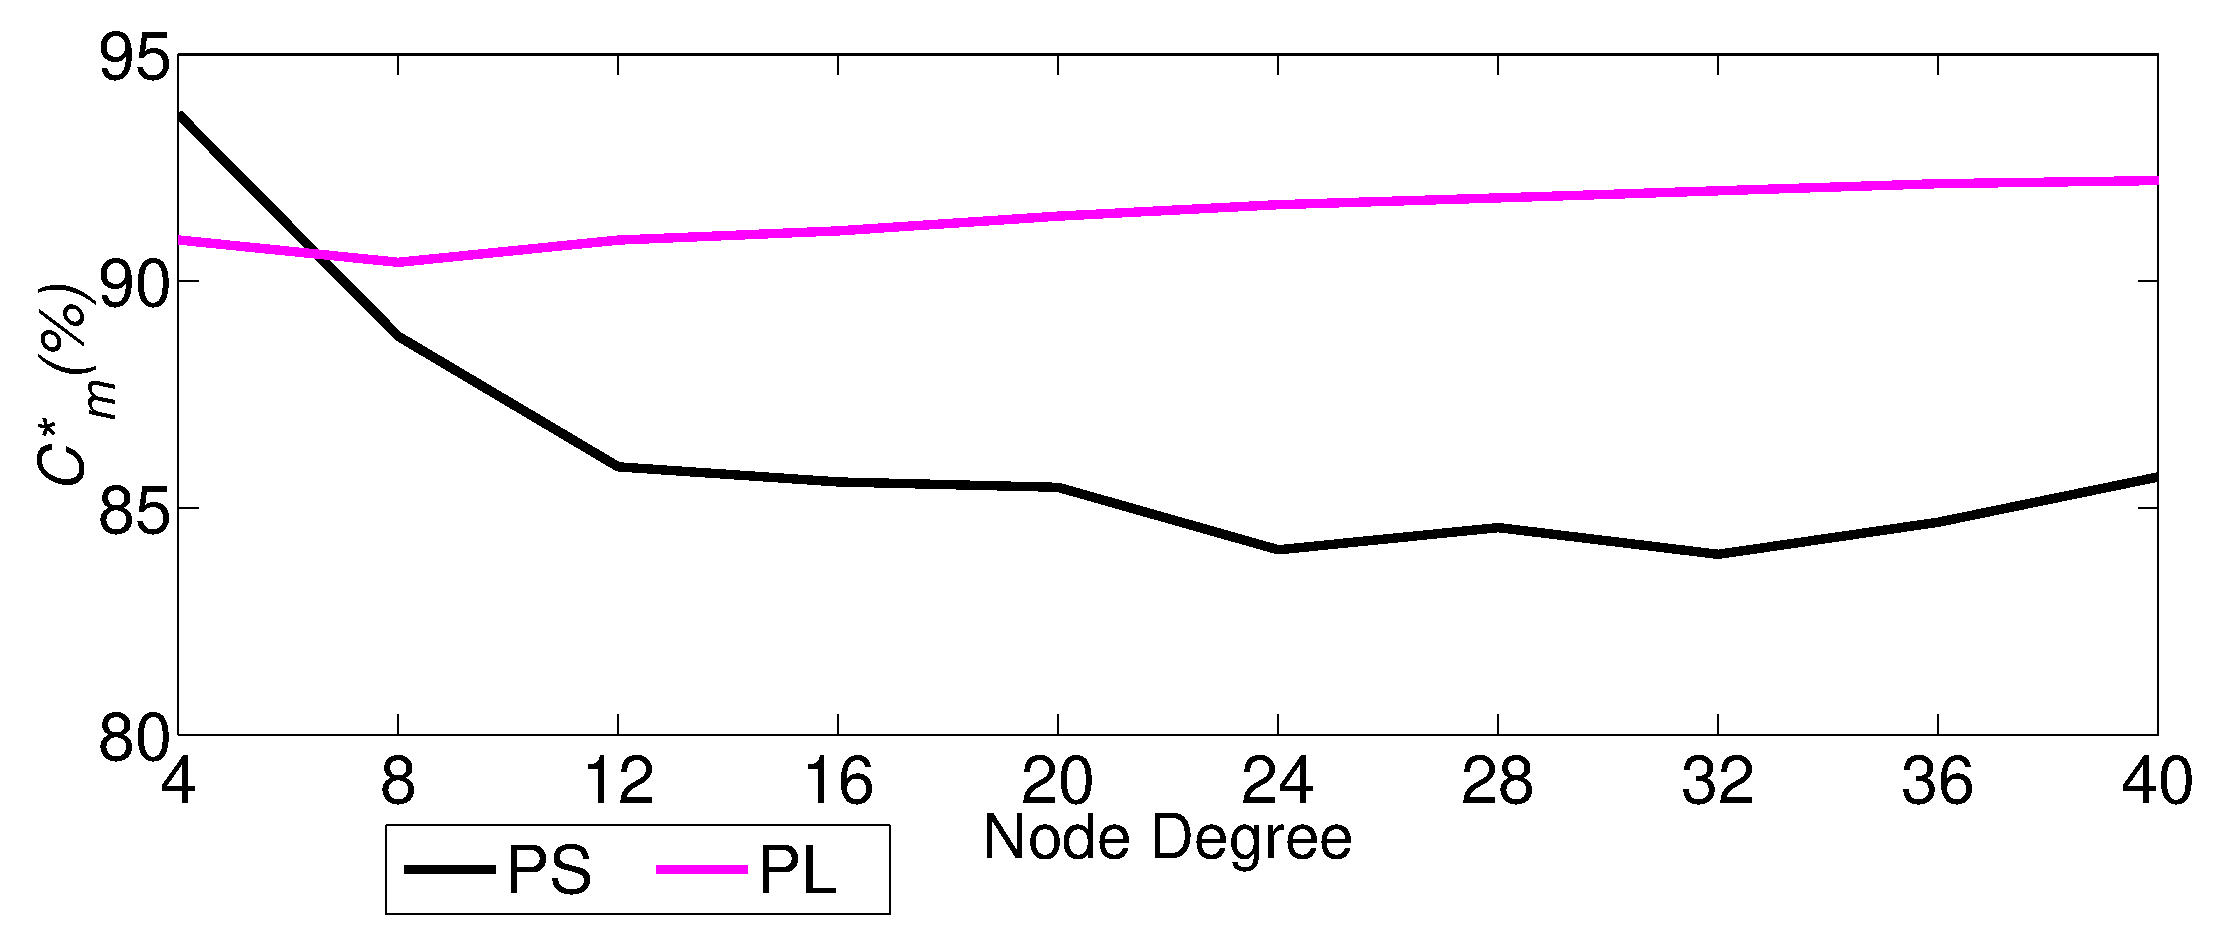
\includegraphics[scale=0.15]{figs1/random_graphs_wastage.eps}
% % \caption{(A) Broadcast time and (B) broadcast wastage versus average degree for B-P . The parameters values are $n=200, m=4, k=2$.\vspace{-3mm}}
% % \label{DiffTopologyGnp_N200_varyD_push_pull}
% % \end{figure}
% % 
% % \begin{figure}
% % \centering
% % \includegraphics[scale=0.4]{diagrams/M2final/DiffTopologyRegularTree_delay_cost_N200_m4_k2_varyD_ps_plRes.eps}
% % \caption{(A) Broadcast time and (B) broadcast wastage versus different values of $d$ for B-P. The parameters values are $n=200, m=4, k=2$.\vspace{-3mm}}
% % \label{DiffTopologyTree_N200_varyD_push_pull}
% % \end{figure}
% \vspace{-3mm}
%  \subsection{Random graph}
%  Here, we assume a random graph topology $G(n, p)$ where $n = 200$, $m = 4$ and $k=2$. Here we vary the probability $p$ of connection (equivalently the average degree $d$) from values ranging from 0.02 to 0.2 (the value of $d$ equivalently varies from 4 to 40) (see figure~\ref{DiffTopologyGnp_N200_varyD_push_pull}). Once again the same observation that both the broadcast time and the broadcast wastage become significantly low for a certain value of $d$ also hold in this case and for this value of $p$ the broadcast time is found to scale as $\log{(n)}$. 
% 
% Thus irrespective of the topology we are able to find a critical value of average degree for the network for which the dynamics becomes as fast as epidemic routing 
% even for the blind push case. Therefore for designing a topology for a network we recommend that the designers look for such a critical value of average degree 
% for which the dynamics becomes fast.
% 
% % \begin{figure}
% % \centering
% % 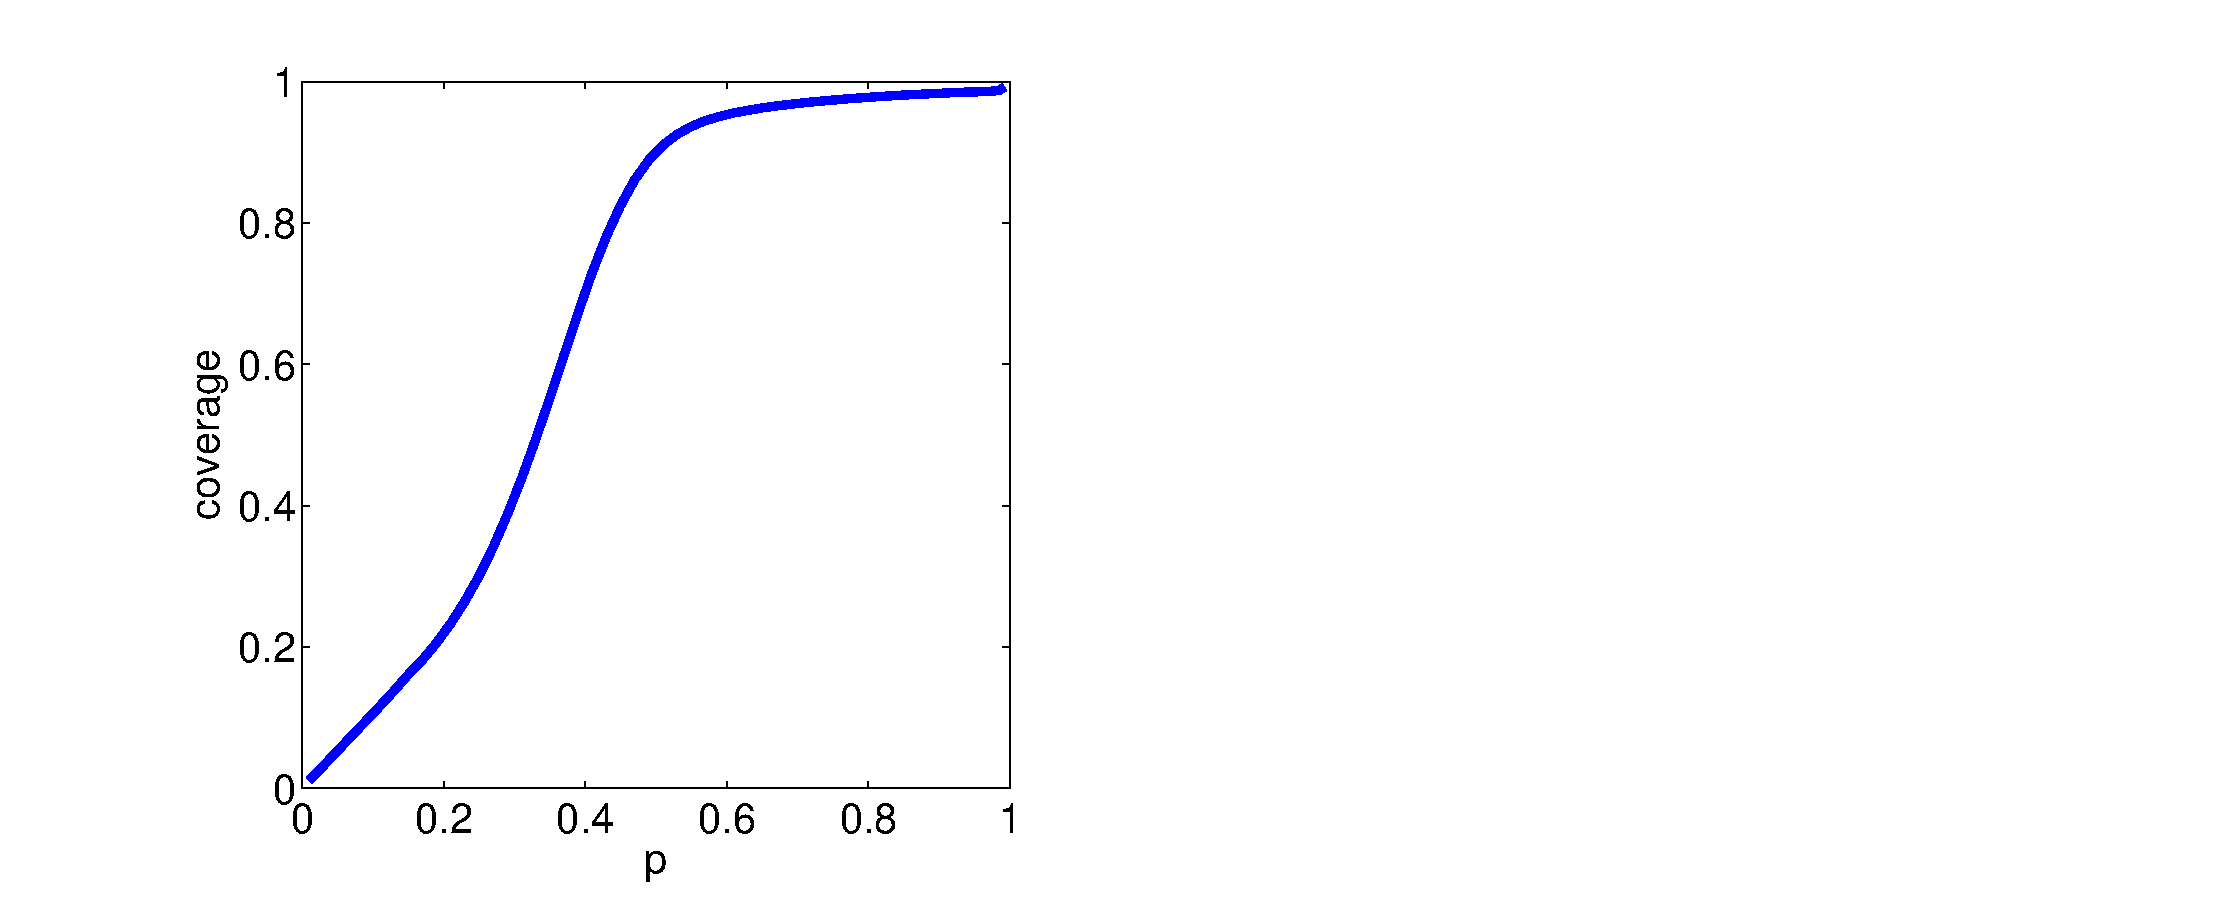
\includegraphics[scale=0.4]{figs1/pvsco.eps}
% % \caption{$p$ versus coverage for gnutella1 network, broadcast technique -- P-P-G \vspace{-3mm}}
% % \label{pcov}
% % \end{figure}

% Since the value of the critical average degree is found to be on the lower side, we performed simulations on sparser variants of the real traces (used previously) 
% and observed that broadcast time reduces even for the B-P. We considered each gnutella snapshot and randomly removed some of the edges such that the 
% network remains connected while producing a sparser variant. From figure ~\ref{gnutellasparse} we observe that the broadcast time reduces significantly 
% in case of the sparser variants in comparison to the original network. 
% Hence, while designing a network it is advisable to keep the network sparse rather than creating unnecessary connections between the nodes. 
% This, as our results indicate, should lead to a faster dissemination of messages.
% \begin{figure}
% \centering
% 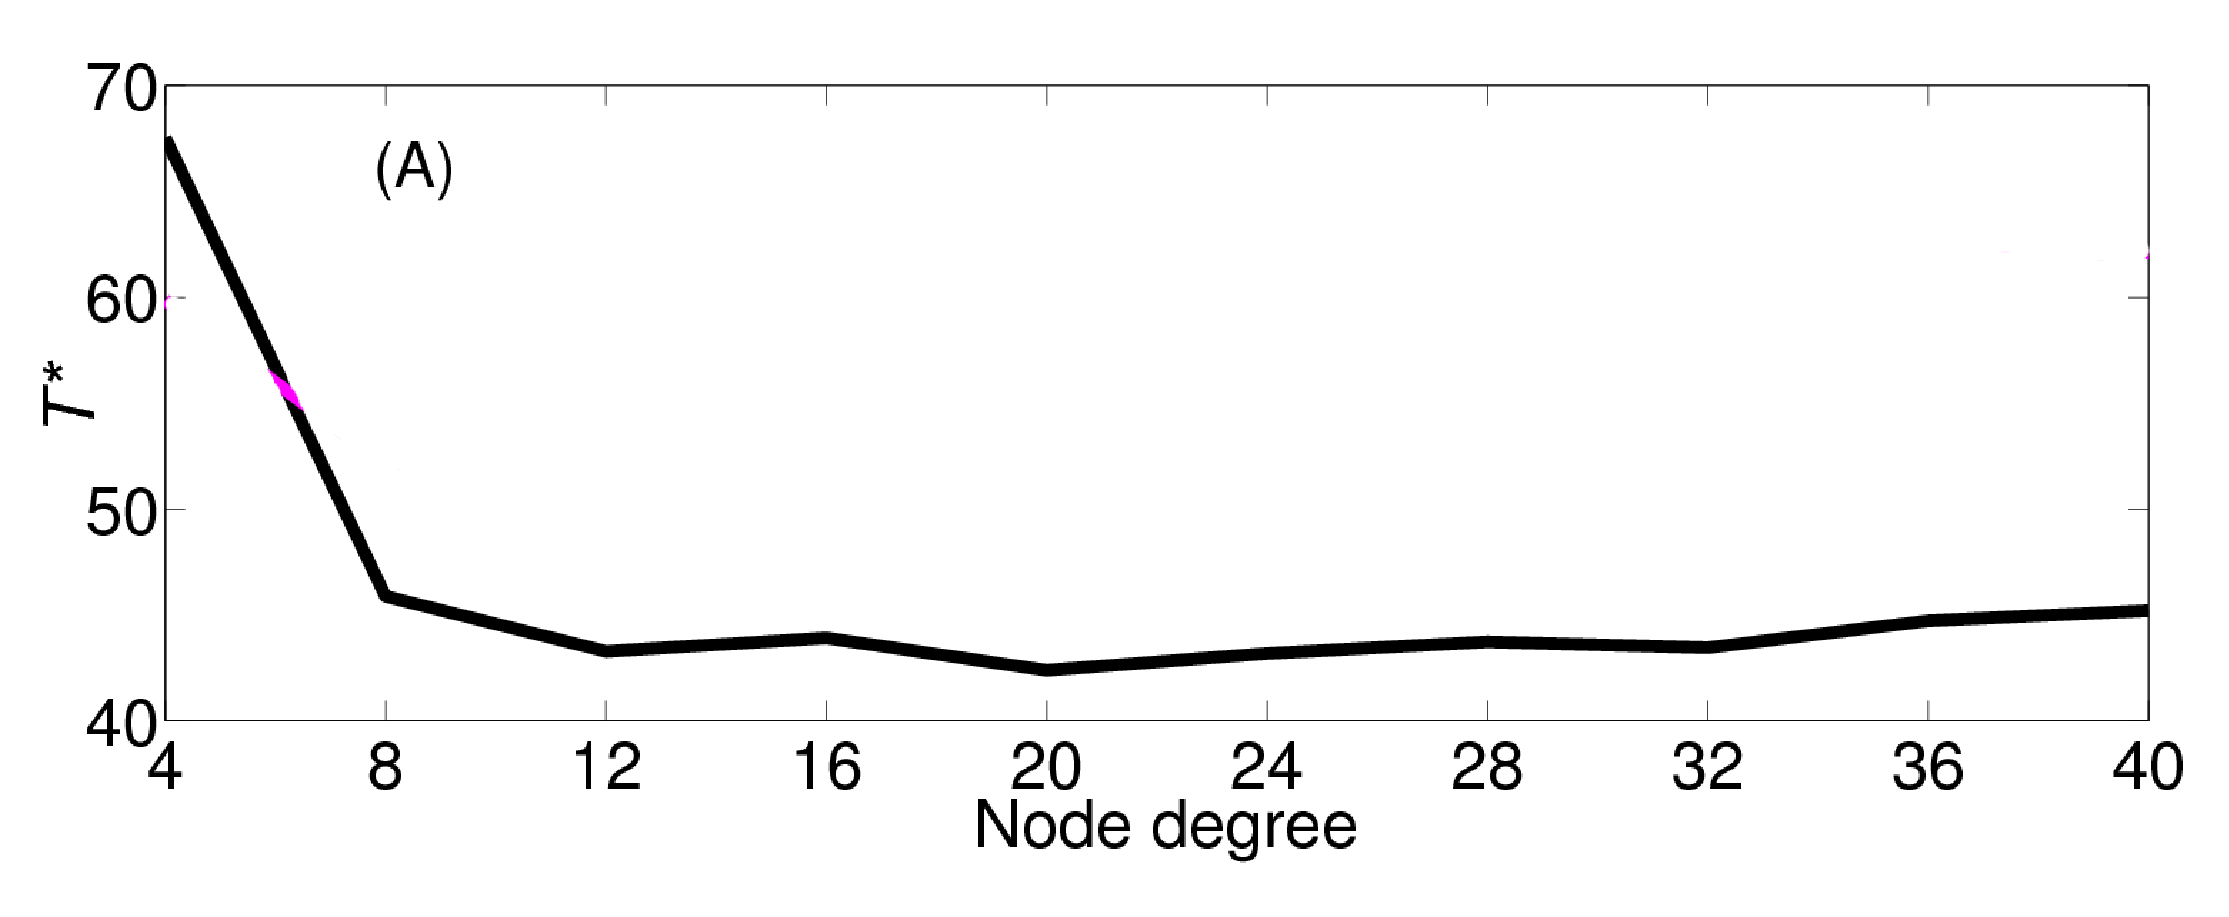
\includegraphics[scale=0.15]{figs1/random_graphs_delay1.eps}
% 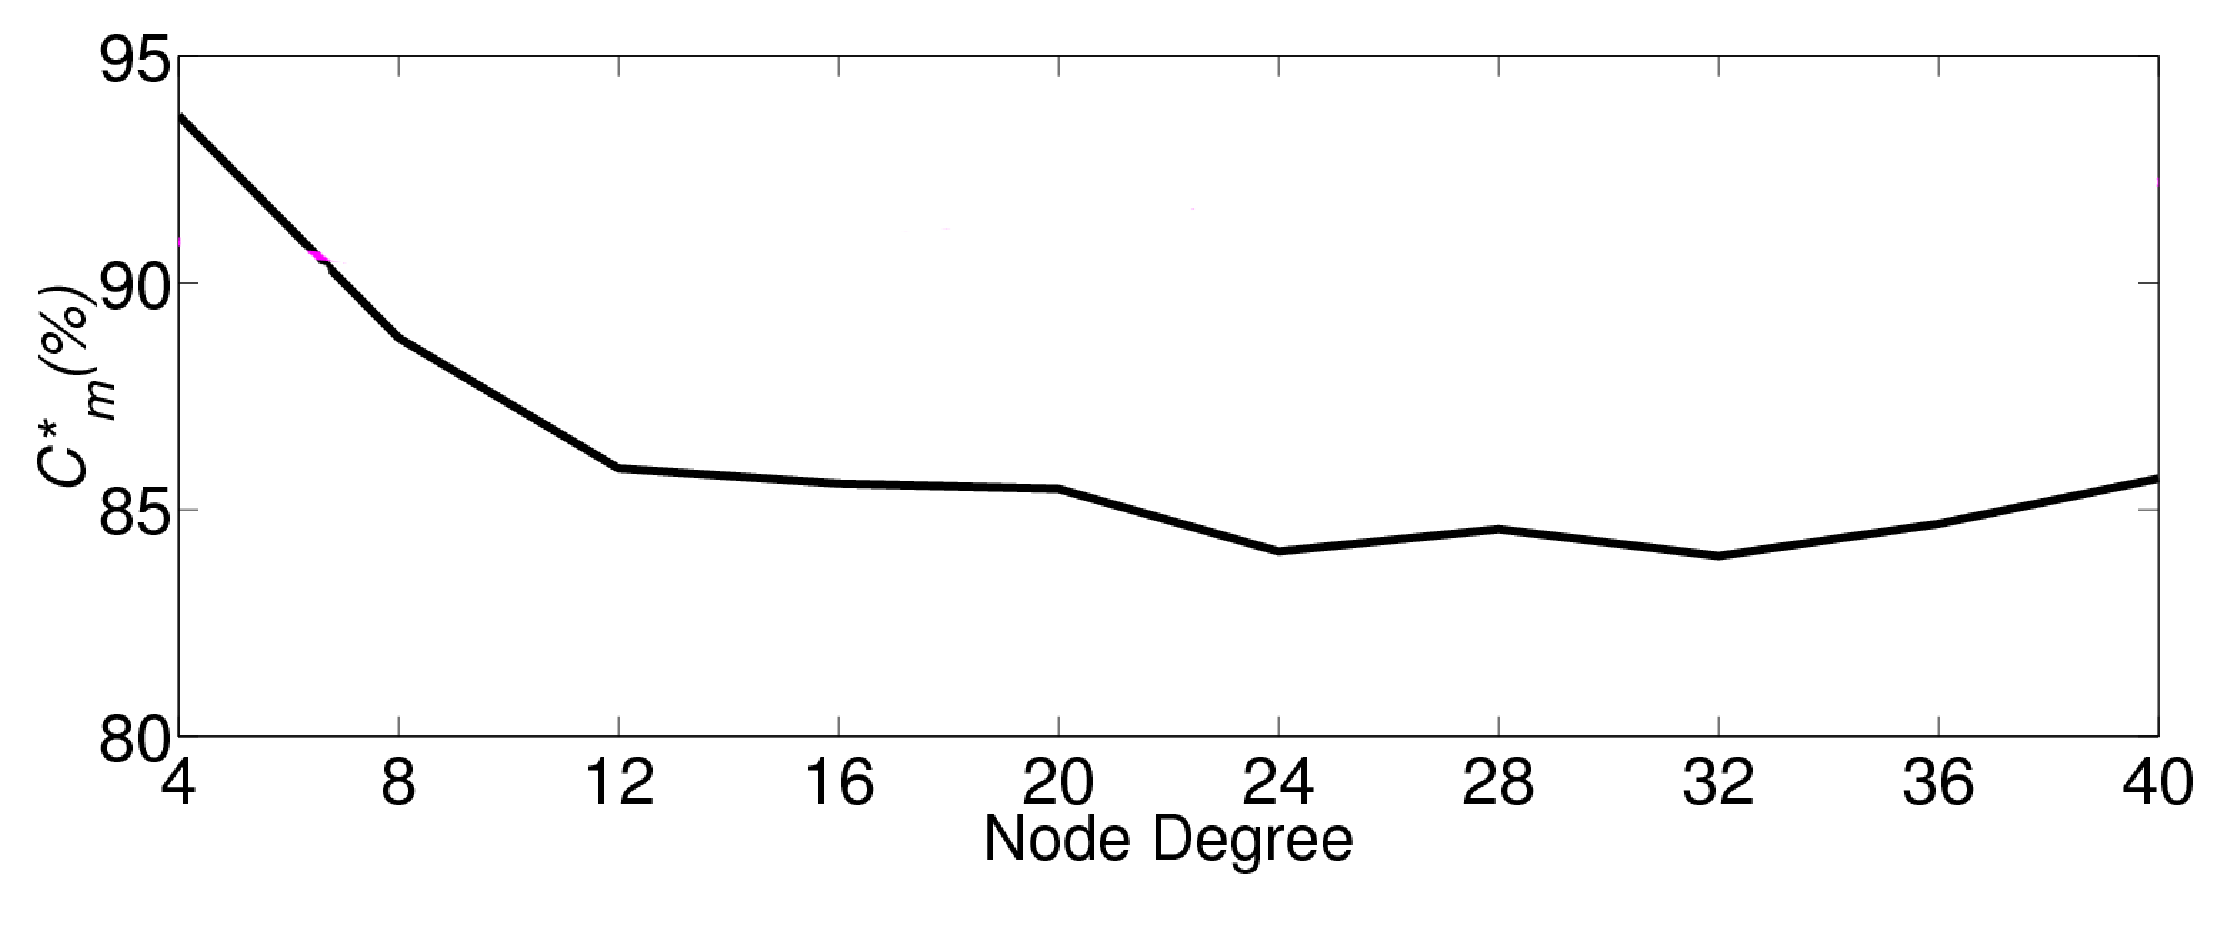
\includegraphics[scale=0.15]{figs1/random_graphs_wastage1.eps}
% \caption{(A) Broadcast time and (B) broadcast wastage versus average degree for B-P . The parameters values are $n=200, m=4, k=2$.\vspace{-3mm}}
% \label{DiffTopologyGnp_N200_varyD_push_pull}
% \end{figure}

\begin{figure}
\centering
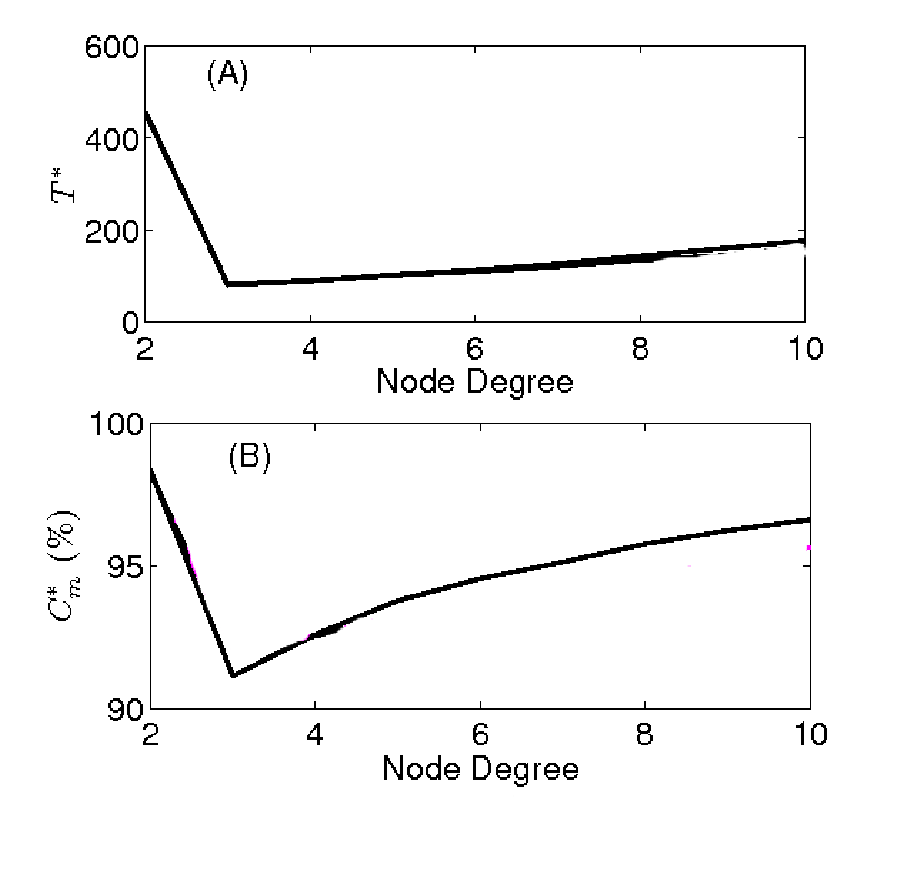
\includegraphics[scale=0.4]{./texfiles/Chapter_3/netsci/figs1/DiffTopologyRegularTree_delay_cost_N200_m4_k2_varyD_ps_plRes1.eps}
\caption{(A) Broadcast time and (B) broadcast wastage versus different values of $d$ for B-P. The parameters values are $n=200, m=4, k=2$.}
\label{DiffTopologyTree_N200_varyD_push_pull}
\end{figure}
%\subsection{Random graph}
%In this section, we assume a random graph topology $G(n, p)$ where $n = 200$, $m = 4$ and $k=2$. Here we vary the probability $p$ of connection (equivalently the average degree $d$) from values ranging from 0.02 to 0.2 (the value of $d$ equivalently varies from 4 to 40) (see figure~\ref{DiffTopologyGnp_N200_varyD_push_pull}). Once again the same observation that both the broadcast time and the broadcast wastage become significantly low for a certain value of $d$ also hold in this case and for this value of $p$ the broadcast time is found to scale as $\log{(n)}$. 

\begin{figure}
\centering
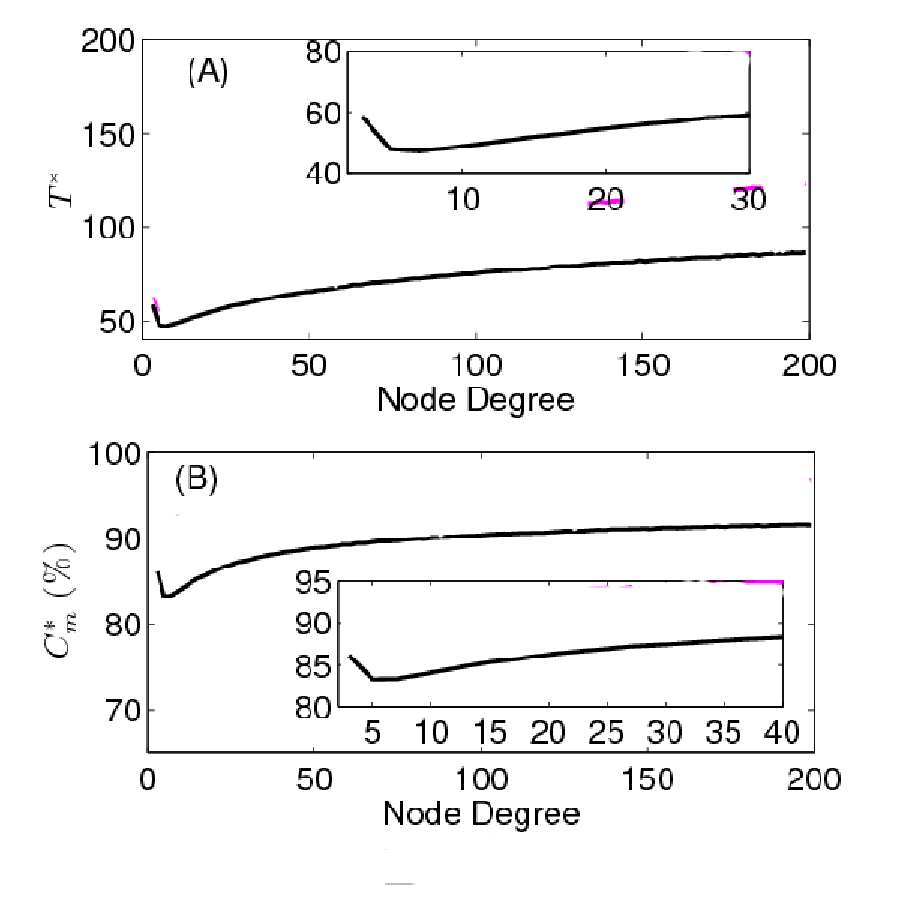
\includegraphics[scale=0.35]{./texfiles/Chapter_3/netsci/figs1/DiffTopology_varyN200_varyD_push_pullRes_m4_k21.eps}
\caption{(A) Broadcast time and (B) broadcast wastage versus different values of $d$ for B-P technique. The parameters values are $n=200, m=4, k=2$. The inset in both the figures show the metrics of interest for the first few values of $d$ to indicate the critical $d$ more appropriately.}
\label{DiffTopologyGraph_N200_varyD_push_pull}
\end{figure}



% \begin{figure}
% \centering
% 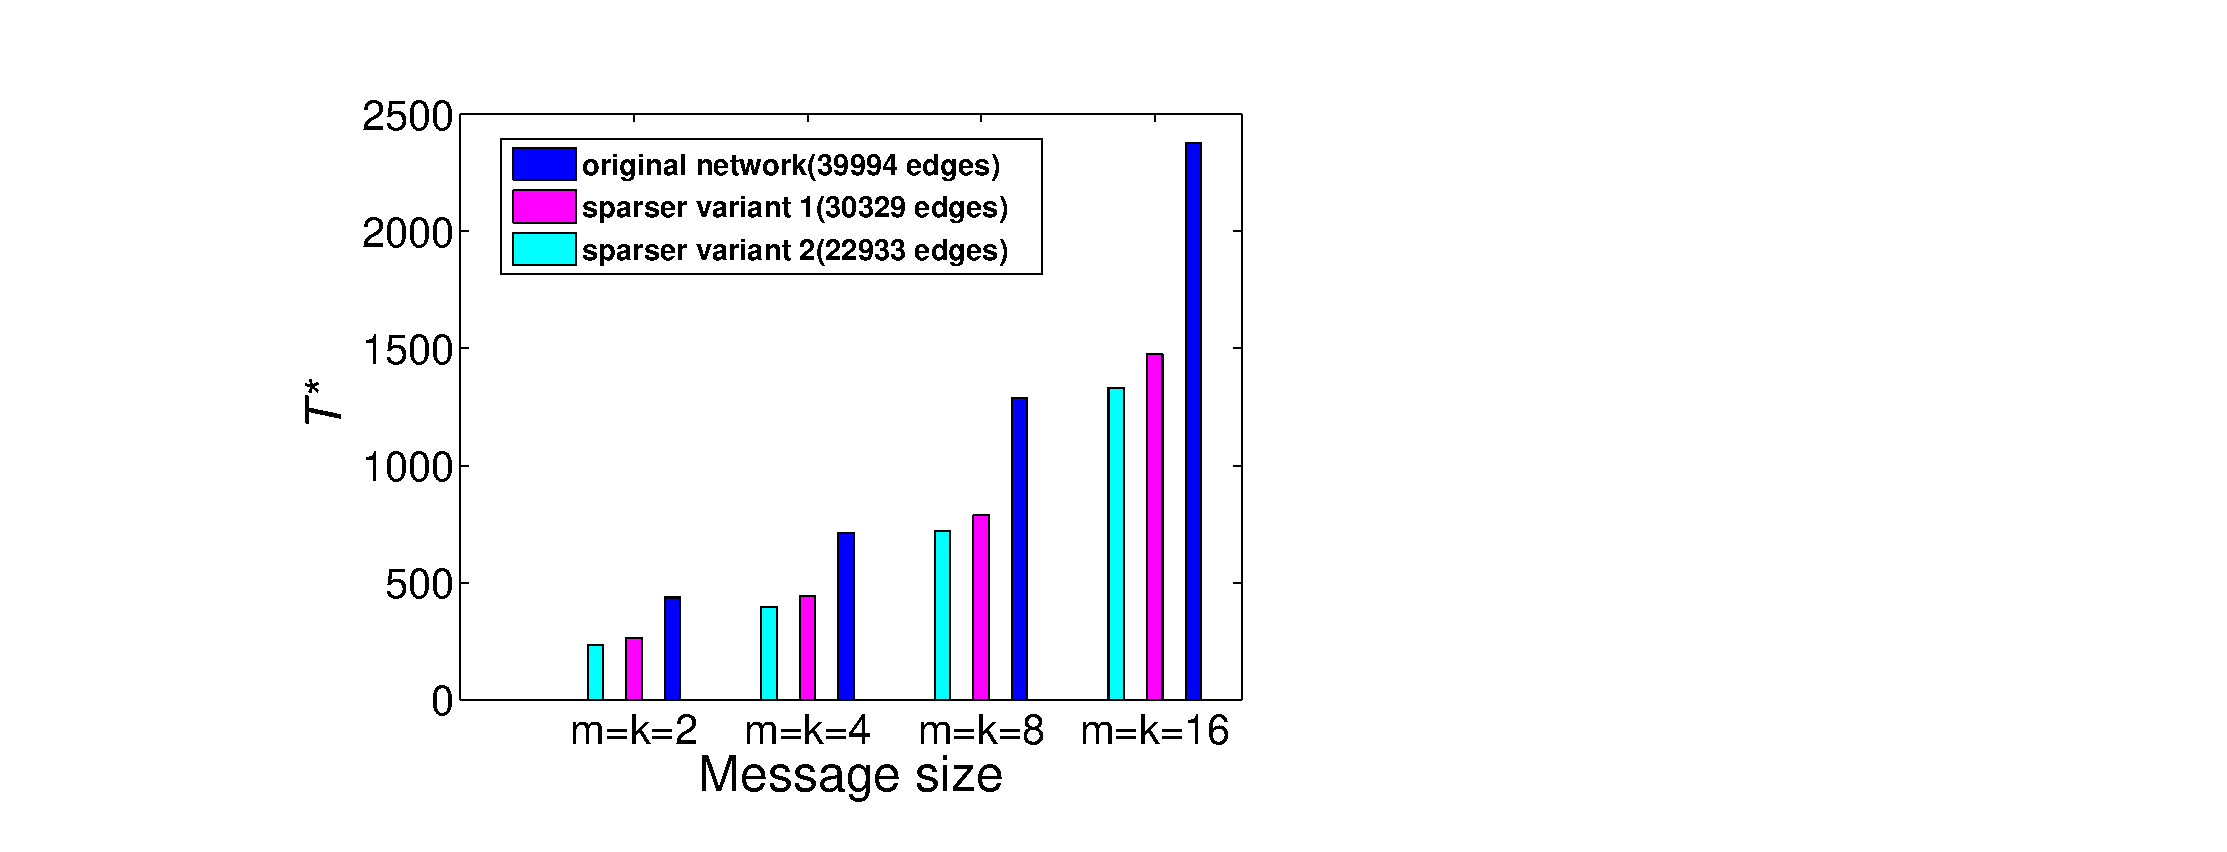
\includegraphics[scale=0.25]{figs1/gnutella1.eps}
% 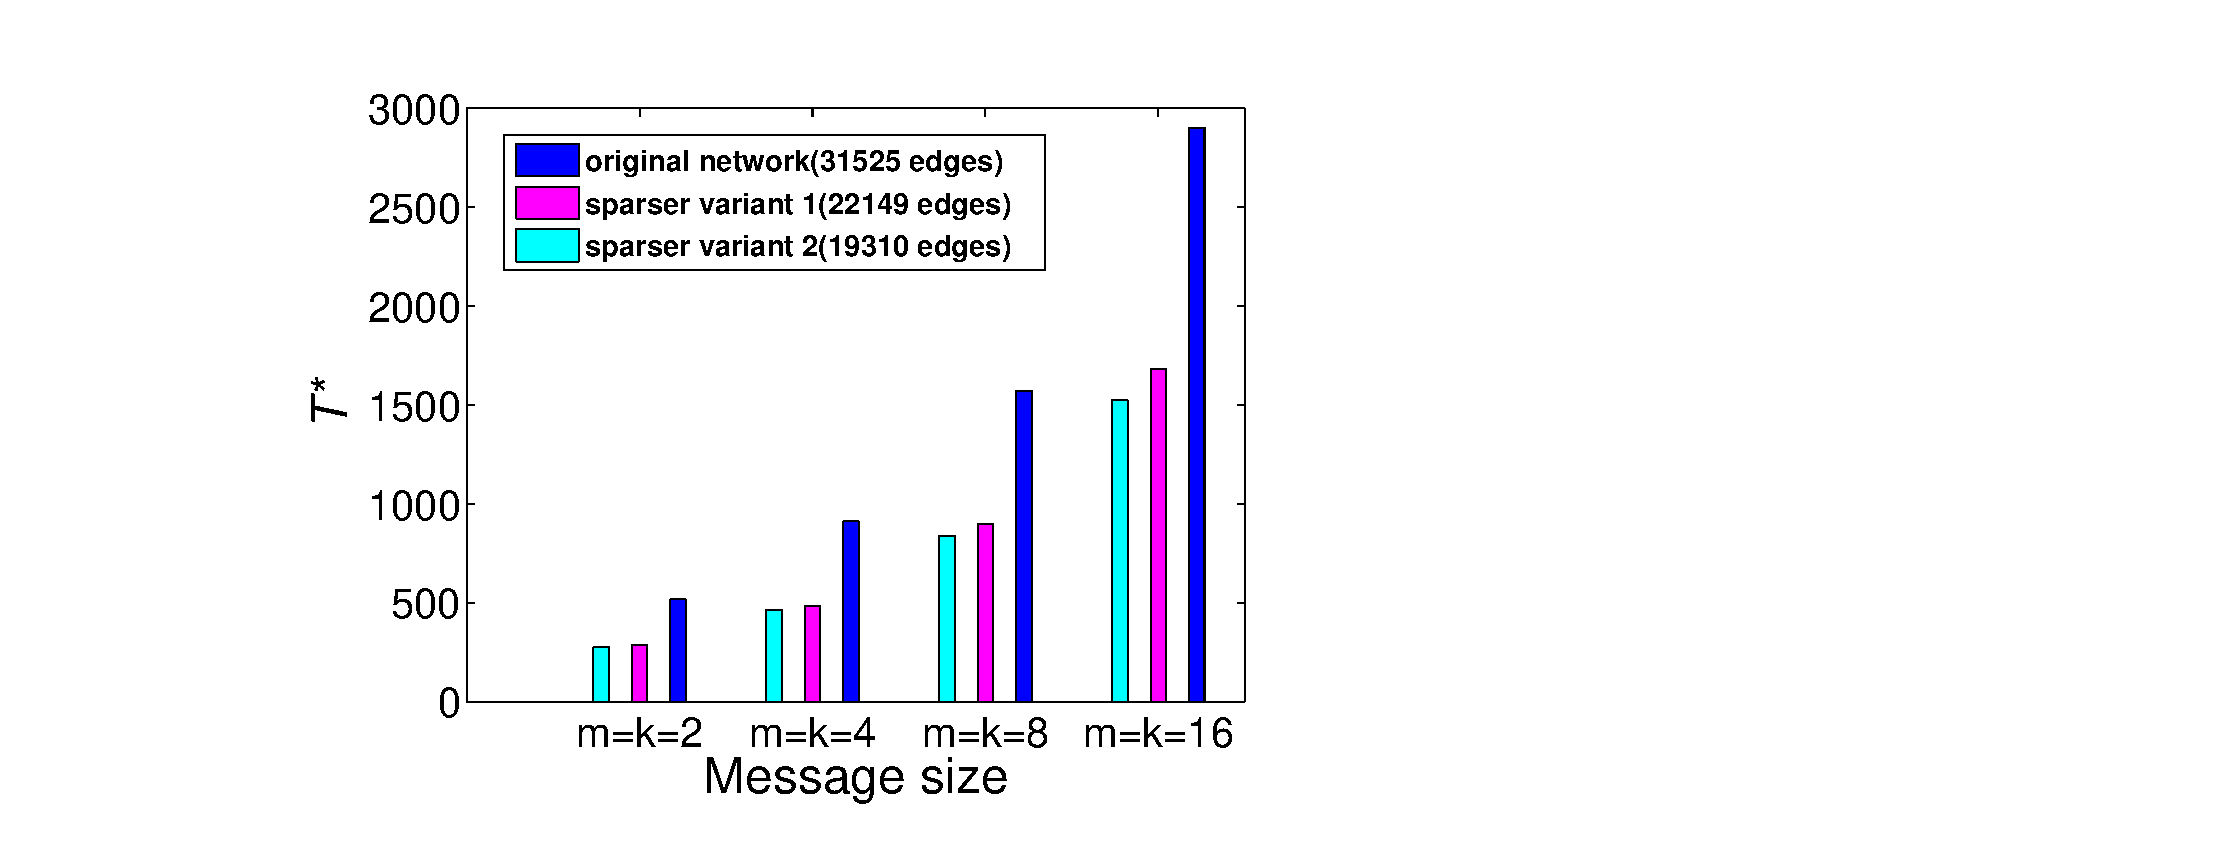
\includegraphics[scale=0.25]{figs1/gnutella2.eps}
% \caption{Broadcast time for the gnutella snapshots and their sparser variants versus different values of message sizes for gnutella1 and gnutella2\vspace{-3mm}}
% \label{gnutellasparse}
% \end{figure}
% \medskip

%\vspace{-2.5mm}
\noindent
%\vspace{-8mm}
\subsection{Comparison of different broadcast strategies on gnutella Topology}
%\vspace{-4mm}
% We measure 
% the performance of the four algorithms (B-P, X-P-P, P-G and P-P-G) on three real network traces based on broadcast time, 
% wastage and coverage. The data sets are Gnutella network snapshots namely 
% p2p-Gnutella04 (gnutella1), p2p-Gnutella06 (gnutella2) and p2p-Gnutella25 (gnutella3) ~\cite{leskovec2007graph,ripeanu2002mapping} taken on dates August 4, August 6 and August 25, 2002 respectively. 
% The gnutella1 network has 10876 nodes and 39994 edges in its largest connected component. Corresponding number of nodes and edges in the largest connected component 
% in gnutella2 and gnutella3 are respectively 8717, 31525 and 22663, 54693. We simulate these algorithms for varying message sizes.
% We perform our simulations on peer-to-peer systems specifically as our study can find a major application in such systems.

% For simulating the X-P-P algorithm in particular we first need to obtain the best value of x for each network and then run the simulations for varying message sizes. 
%  In figure ~\ref{ps_bt} and ~\ref{ps_wa}, we show how the broadcast time and wastage varies with x for gnutella1 network. We observe that the best value of x lies around 
%  50\%. Similarly we obtained the value of x for the other two datasets as well and found it to be around 50\% and 60\% for gnutella2 and gnutella3 
%  respectively.
% \begin{figure}
% \centering
% 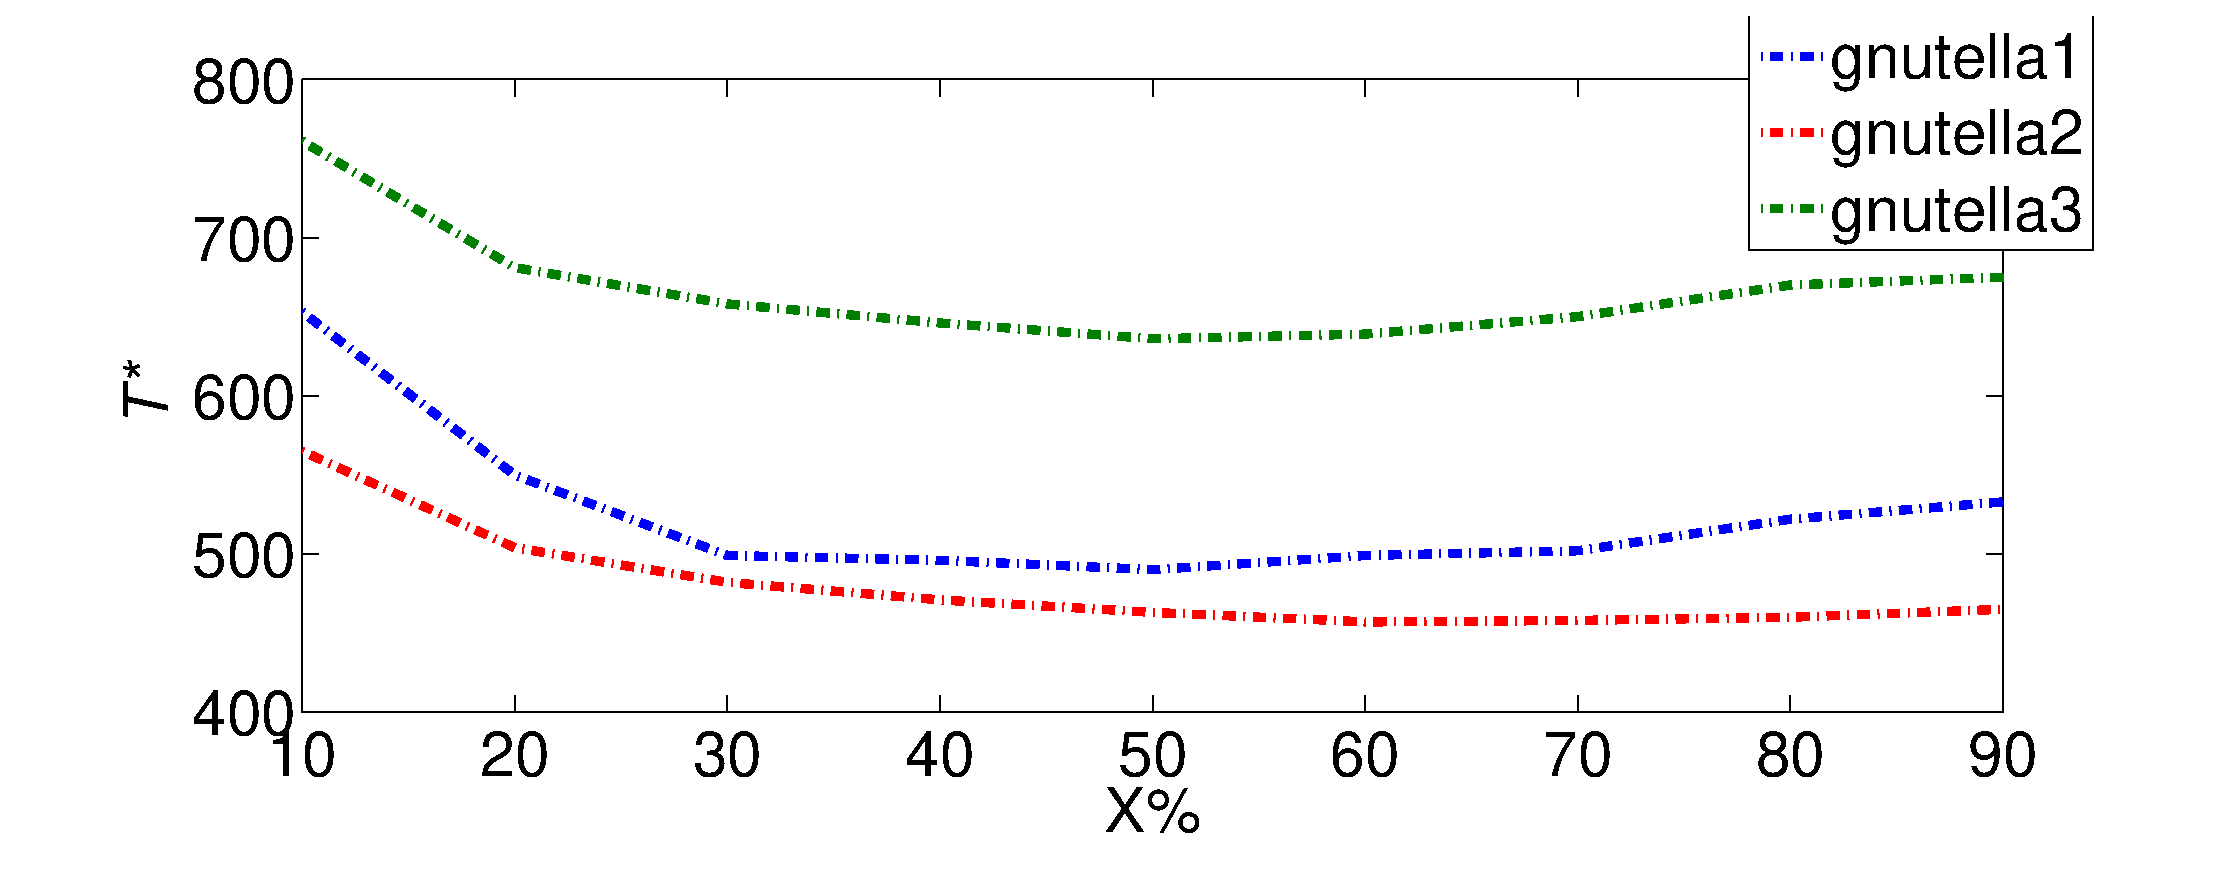
\includegraphics[scale=0.15]{figs1/xperbt.eps}
% 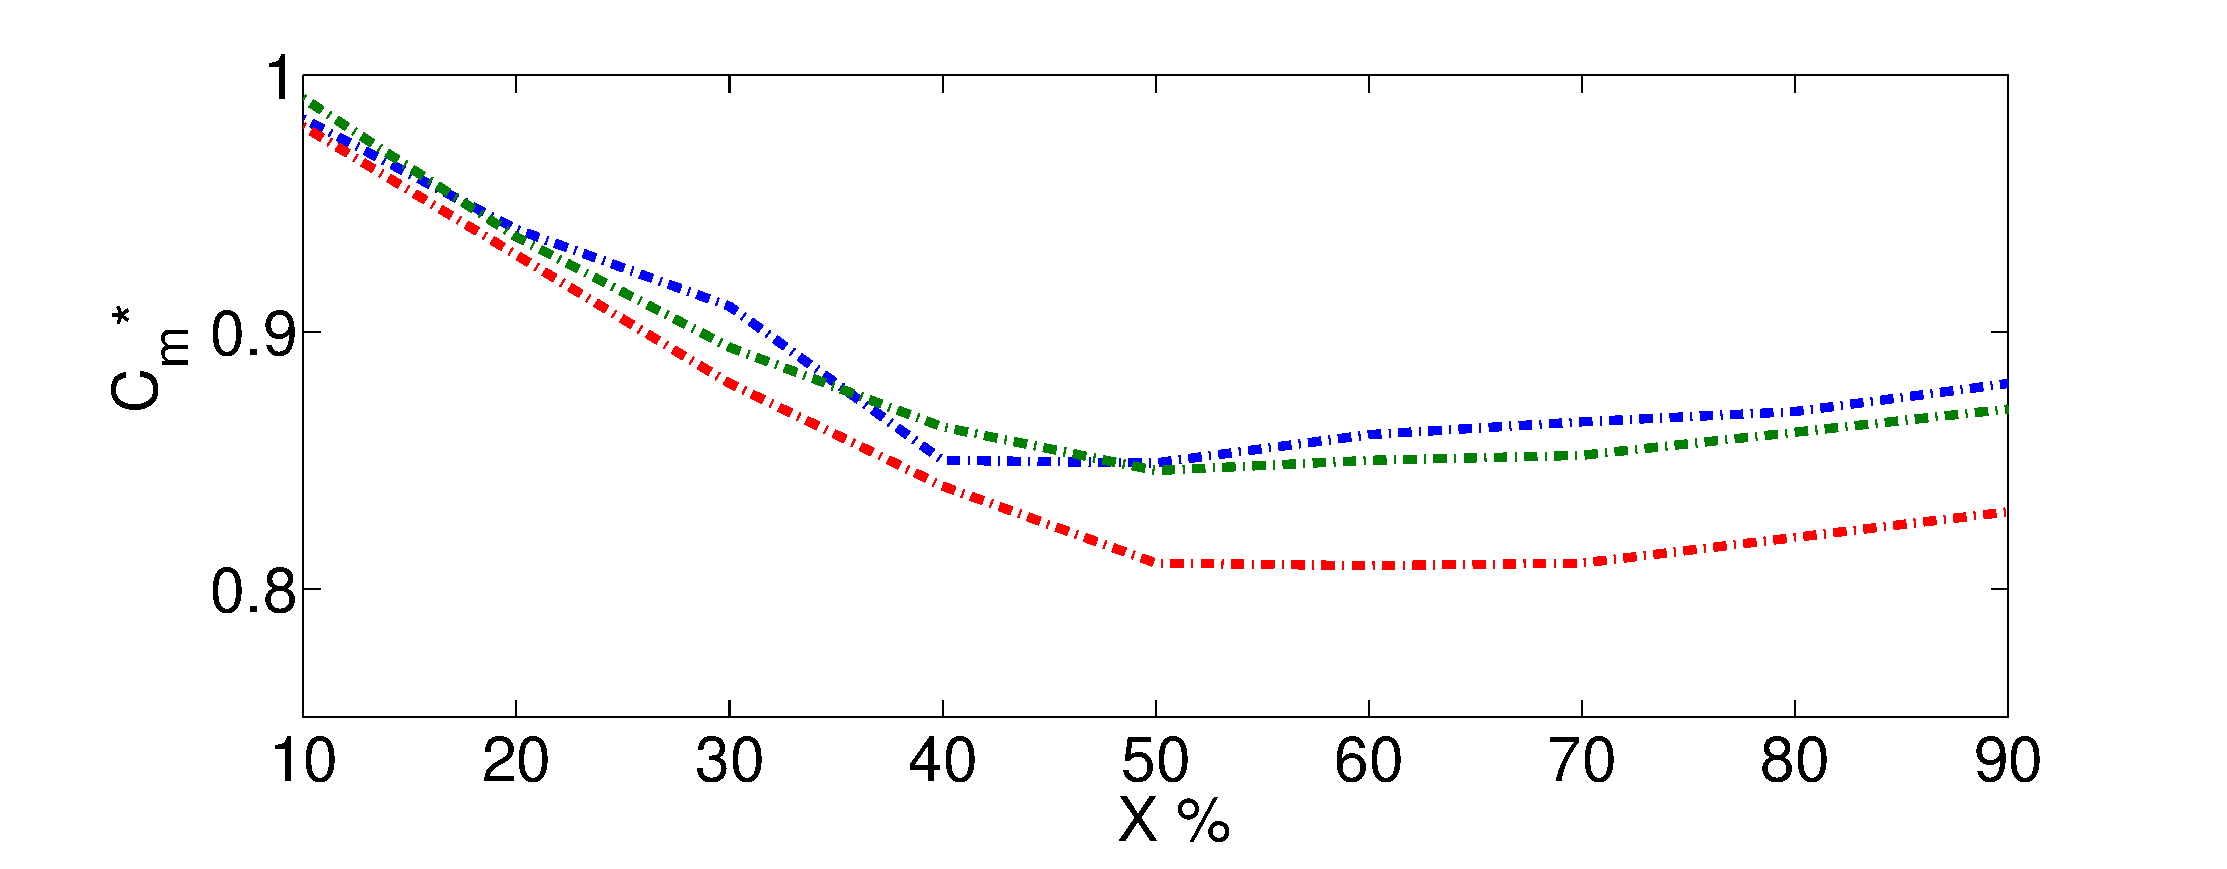
\includegraphics[scale=0.15]{figs1/xperwa.eps}
% \caption{Average broadcast time and wastage versus x for gnutella1,gnutella2 and gnutella3\vspace{-5mm}}
% \label{ps_bt}
% \end{figure}

% \begin{figure}[htpb]
% \centering
% 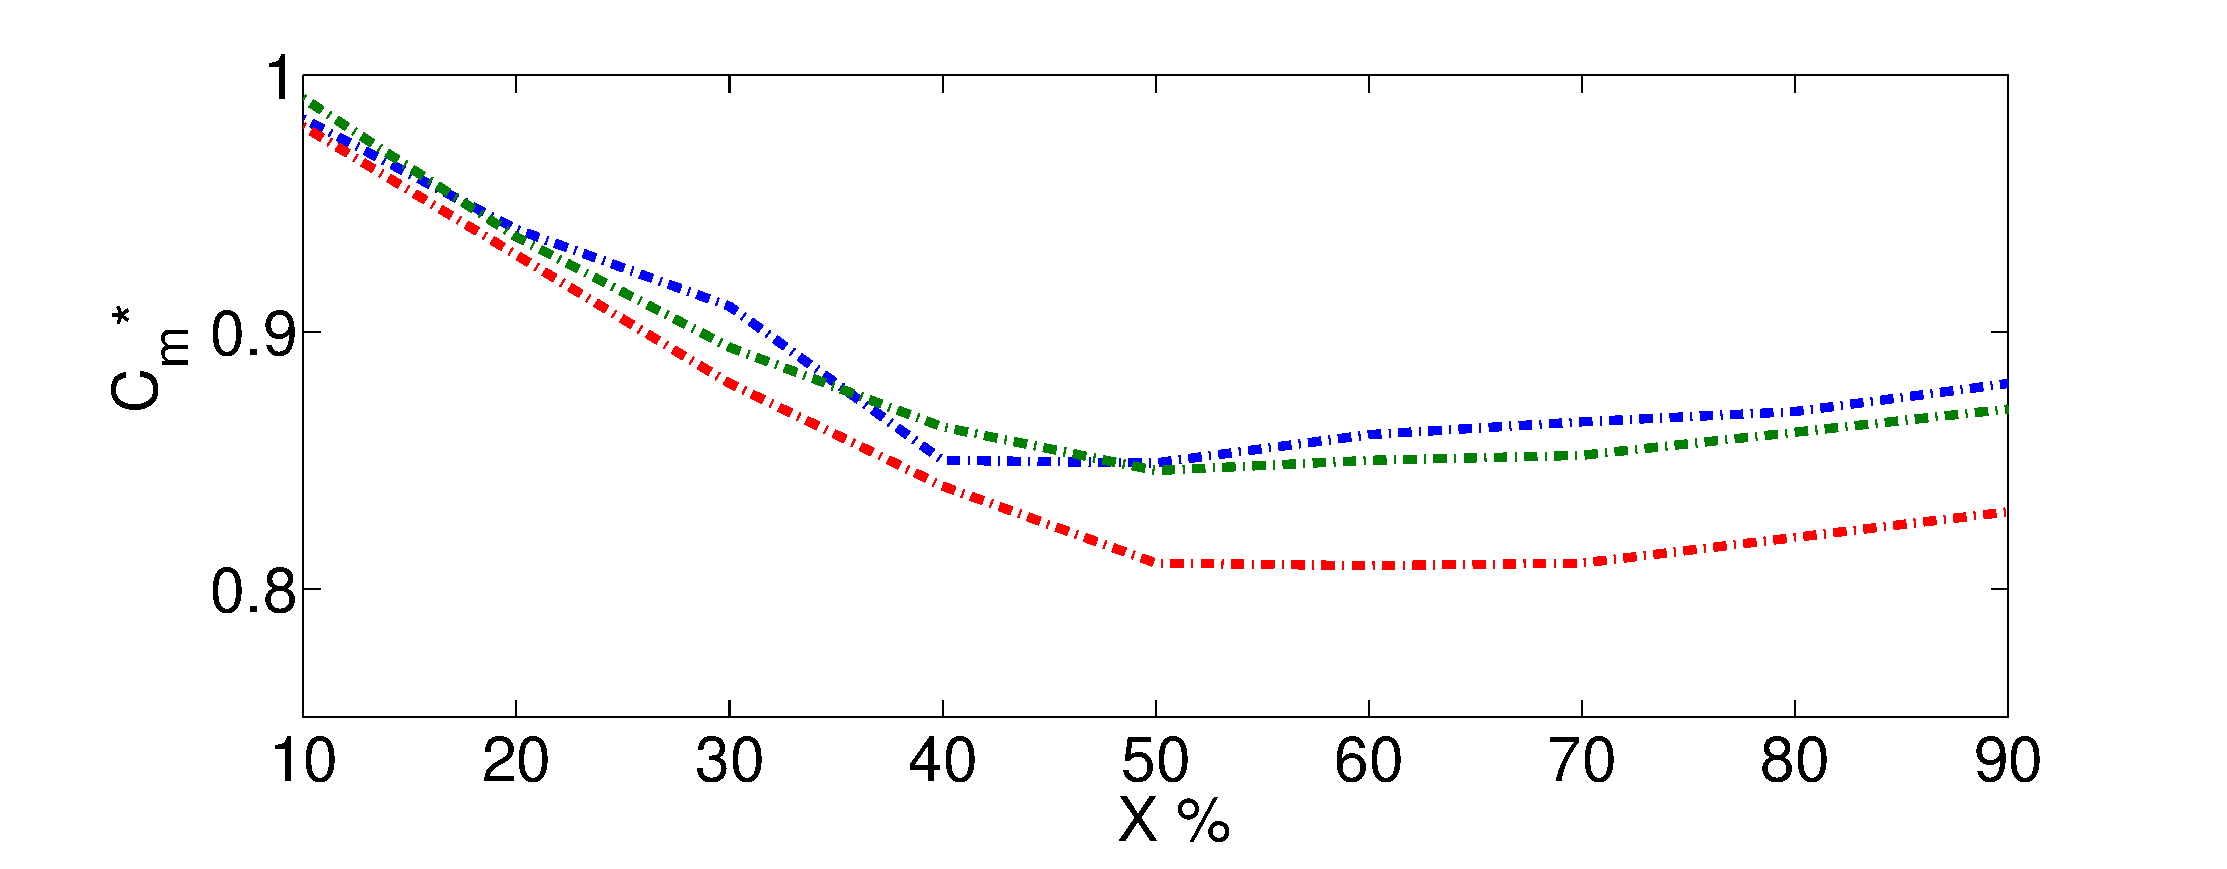
\includegraphics[scale=0.15]{figs1/xperwa.eps}
% \caption{average wastage time versus x for gnutella1\vspace{-5mm}}
% \label{ps_wa}
% \end{figure}
% \begin{figure*}[!ht]
%   \centering
%   \includegraphics*[width=0.65\textwidth,height=40mm,angle=0]{figs1/gnutella4_bt_wa_co.eps}
% 
%  \vspace{-5mm}
%  %\caption{\label{gnutellacomp} (A) broadcast time versus message size (B) wastage versus message size (C) coverage versus message size for gnutella1, gnutella2 and gnutella3}
% \end{figure*}
% \begin{figure*}[!ht]
%   \centering
%  \includegraphics*[width=0.65\textwidth,height=40mm,angle=0]{figs1/gnutella6_bt_wa_co.eps}	
%  \vspace{-5mm}
% 
%  
%  %\caption{\label{gnutellacomp} (A) broadcast time versus message size (B) wastage versus message size (C) coverage versus message size for gnutella1, gnutella2 and gnutella3}
% \end{figure*}
% \begin{figure}
% \centering
% \includegraphics[scale=0.15]{figs1/xperbt.eps}
% \includegraphics[scale=0.15]{figs1/xperwa.eps}
% \caption{Average broadcast time and wastage versus x for gnutella1,gnutella2 and gnutella3\vspace{-5mm}}
% \label{ps_bt}
% \end{figure}
%\medskip

\begin{figure}
\centering
\includegraphics[scale=0.19]{./texfiles/Chapter_3/netsci/figs1/random_graphs_delay1.eps}
\includegraphics[scale=0.18]{./texfiles/Chapter_3/netsci/figs1/random_graphs_wastage1.eps}
\caption{(A) Broadcast time and (B) broadcast wastage versus average degree for B-P. The parameters values are $n=200, m=4, k=2$.\vspace{4mm}}
\label{DiffTopologyGnp_N200_varyD_push_pull}
\end{figure}
\begin{figure}
\centering
\includegraphics[scale=0.19]{./texfiles/Chapter_3/netsci/figs1/xperbt.eps}
\includegraphics[scale=0.19]{./texfiles/Chapter_3/netsci/figs1/xperwa.eps}
\caption{Average broadcast time and wastage versus $x$ for gnutella1, gnutella2 and gnutella3}
\label{ps_bt}
\end{figure}


\begin{figure*}[!ht]
  \centering	
 \includegraphics*[width=0.65\textwidth,height=40mm,angle=0]{./texfiles/Chapter_3/netsci/figs1/gnutella25_bt_wa_co.eps}
%\vspace{-5mm}
 
 \caption{\label{gnutellacomp} (A) Broadcast time versus message size (B) Wastage versus message size (C) Coverage versus message size for gnutella3}
\end{figure*}


\begin{figure*}[!ht]
  \centering	
 \includegraphics*[width=0.45\textwidth,height=40mm,angle=0]{./texfiles/Chapter_3/netsci/figs1/comp_gnut_4.eps}
 \includegraphics*[width=0.45\textwidth,height=40mm,angle=0]{./texfiles/Chapter_3/netsci/figs1/comp_gnut_6.eps}
%\vspace{-5mm}
 
 \caption{\label{gnutellacomp1} Gain in broadcast time of P-P-G over X-P-P and B-P [Inset shows gain in wastage] for (A) gnutella1 and (B) gnutella2 networks. Note: algo = B-P/X-P-P }
\vspace{.5cm}
 \end{figure*}
% \begin{figure*}[!ht]
%   \centering	
%  \includegraphics*[width=0.65\textwidth,height=40mm,angle=0]{figs1/gnutella25_bt_wa_co.eps}
% \vspace{-5mm}
%  
%  \caption{\label{gnutellacomp} (A) Broadcast time versus message size (B) Wastage versus message size (C) Coverage versus message size for gnutella1, gnutella2 and gnutella3\vspace{-3mm}}
% \end{figure*}

We measure 
the performance of the algorithms (B-P, X-P-P and P-P-G) on three real network traces based on broadcast time, 
wastage and coverage. The data sets are Gnutella network snapshots namely 
p2p-Gnutella04 (gnutella1), p2p-Gnutella06 (gnutella2) and p2p-Gnutella25 (gnutella3)~\cite{leskovec2007graph,ripeanu2002mapping} taken on dates August 4, August 6 and August 25, 2002 respectively. 
The gnutella1 network has 10876 nodes and 39994 edges in its largest connected component. Corresponding number of nodes and edges in the largest connected component 
in gnutella2 and gnutella3 are respectively 8717, 31525 and 22663, 54693. We simulate these algorithms for varying message sizes.
We perform our simulations on peer-to-peer systems specifically as our study can find a major application in such systems.

For simulating the X-P-P algorithm in particular we first need to obtain the best value of $x$ for each network and then run the simulations for varying message sizes. 
 In figure~\ref{ps_bt}, we show how the broadcast time and wastage varies with $x$ for networks gnutella1, gnutella2 and gnutella3. We observe that the best value of $x$ lies around 
 50\% for the gnutella1 network. Similarly the obtained value of $x$ are found to be around 50\% and 60\% for gnutella2 and gnutella3 
 respectively.
% We measure the performance of the three algorithms (B-P, P-G and P-P-G) on three real network traces based on broadcast time, 
% wastage and coverage. The data sets are Gnutella snapshots namely 
% p2p-Gnutella04 (gnutella1), p2p-Gnutella06 (gnutella2) and p2p-Gnutella25 ~\cite{ripeanu2002mapping,leskovec2007graph} taken on dates August 4, August 6 and August 25, 2002 respectively. 
% The gnutella1 network has 10876 nodes and 39994 edges in its largest connected component. Corresponding number of nodes and edges in the largest connected component 
% in gnutella2 and gnutella3 are respectively 8717, 31525 and 22663, 54693. We simulate these algorithms for varying message sizes.
% 
% For simulating the X-P-P algorithm we first obtain the best value of x for each network and then run the simulations for varying message sizes. 
%  In figure ~\ref{ss} and ~\ref{}, we show how the broadcast time and wastage varies with x for gnutella1 network. We obsreve that the best value of x lies around 
%  50\%. Similarly we obtained the value of x for the other two datasets as well and found it to be around 50\% and 60\% for gnutella2 and gnutella3 
%  respectively.
% As mentioned earlier we observe from simulation results (shown in figure [4]) that the P-G algorithm performs better than B-P with respect to broadcast time and 
%  wastage with a reasonably good coverage of around 95\% when message size is 2. However, the coverage drastically falls as we increase the message size. 
%  P-P-G performs best among all the algorithms in terms of broadcast time.
%  It is so because the non-sender nodes are allowed $pull$ opportunities in addition to $push$ by 
%  sender nodes. In addition, it can be noticed that the overall wastage with respect to B-P is also reduced significantly. 
%  X-P-P performs best in terms of wastage and is second only to P-P-G in terms of broadcast time. Actually, X-P-P provides the best optimization 
%   between broadcast time and wastage but would incur significant computational overhead if implemented; in fact, it is infeasible in practical distributed settings.
%  Note that it is almost impossible to have an algorithm which optimizes both broadcast time and wastage yet providing maximum coverage.
%  Our proposed algorithm (P-P-G) presents the best possible trade-off of delay and wastage guaranteeing almost 100\% coverage and can be 
%  implemented in a distributed fashion with almost negligible computational overhead.
In figure ~\ref{gnutellacomp} we plot the broadcast time, wastage and coverage for gnutella3 network. 
We observe that with P-P-G we gain in both broadcast time and wastage with respect to B-P. With respect to X-P-P, P-P-G offers better 
broadcast time but with a higher wastage.
For gnutella1 and gnutella2 networks 
we plot (figure ~\ref{gnutellacomp1}) the ratio of broadcast time and wastage of X-P-P and B-P over P-P-G for different message sizes. 
% We observe that accross different message sizes on an average the ratio of broadcast time of X-P-P over P-P-G is around $1.5$ and that for B-P over P-P-G is $5.8$. 
% The corresponding values for wastage are $0.75$ and $1.10$ respectively. 
We observe that across different message sizes, on average the increase in broadcast time of X-P-P over P-P-G and B-P over P-P-G are $5.45$ and $1.5$ respectively for 
gnutella1 network while for gnutella2 network the corresponding values are 5.9 and 1.6 respectively. Corresponding values for wastage are $0.75$ and $1.10$ 
respectively for gnutella1 network and $0.72$ and $1.06$ respectively for gnutella2 network. 
So with P-P-G we gain in both broadcast time and wastage with respect to B-P while with respect to X-P-P 
we gain in broadcast time without significant increase in wastage.
 Actually, X-P-P provides the best optimization between broadcast time and wastage but it would be hard to implement in a 
distributed setting. 
Our proposed algorithm (P-P-G) presents the best possible trade-off between delay and wastage guaranteeing almost 100\% coverage and can be implemented in a distributed fashion with almost negligible computational overhead.
% \begin{figure*}[!ht]
%   \centering
%   \includegraphics*[width=0.65\textwidth,height=40mm,angle=0]{figs1/gnutella4_bt_wa_co.eps}
% 
%  \vspace{-5mm}
%  %\caption{\label{gnutellacomp} (A) broadcast time versus message size (B) wastage versus message size (C) coverage versus message size for gnutella1, gnutella2 and gnutella3}
% \end{figure*}
% \begin{figure*}[!ht]
%   \centering
%  \includegraphics*[width=0.65\textwidth,height=40mm,angle=0]{figs1/gnutella6_bt_wa_co.eps}	
%  \vspace{-5mm}
% 
%  
%  %\caption{\label{gnutellacomp} (A) broadcast time versus message size (B) wastage versus message size (C) coverage versus message size for gnutella1, gnutella2 and gnutella3}
% \end{figure*}
% 
% \begin{figure*}[!ht]
%   \centering	
%  \includegraphics*[width=0.45\textwidth,height=40mm,angle=0]{figs1/comp_gnut_4.eps}
%  \includegraphics*[width=0.45\textwidth,height=40mm,angle=0]{figs1/comp_gnut_6.eps}
% \vspace{-5mm}
%  
%  \caption{\label{gnutellacomp1} Efficiency in broadcast time of P-P-G over X-P-P and B-P for gnutella1 and gnutella2 networks. (inset) efficiency in wastage of P-P-G over X-P-P and P-G \vspace{-10mm}}
% \end{figure*}
% We measure the performance of the three algorithms (B-P, P-G and P-P-G) on three real network traces based on broadcast time, 
% wastage and coverage. The data sets are Gnutella snapshots namely 
% p2p-Gnutella04 (gnutella1), p2p-Gnutella06 (gnutella2) and p2p-Gnutella25 ~\cite{ripeanu2002mapping,leskovec2007graph} taken on dates August 4, August 6 and August 25, 2002 respectively. 
% The gnutella1 network has 10876 nodes and 39994 edges in its largest connected component. Corresponding number of nodes and edges in the largest connected component 
% in gnutella2 and gnutella3 are respectively 8717, 31525 and 22663, 54693. We simulate these algorithms for varying message sizes.

% \begin{figure*}[!ht]
%   \centering
%   \includegraphics*[width=0.7\textwidth,height=55mm,angle=0]{figs1/gnutella4_bt_wa_co.eps}
% 
%  \vspace{-5mm}
%  %\caption{\label{gnutellacomp} (A) broadcast time versus message size (B) wastage versus message size (C) coverage versus message size for gnutella1, gnutella2 and gnutella3}
% \end{figure*}
% \begin{figure*}[!ht]
%   \centering
%  \includegraphics*[width=0.7\textwidth,height=55mm,angle=0]{figs1/gnutella6_bt_wa_co.eps}	
%  \vspace{-5mm}
% 
%  
%  %\caption{\label{gnutellacomp} (A) broadcast time versus message size (B) wastage versus message size (C) coverage versus message size for gnutella1, gnutella2 and gnutella3}
% \end{figure*}
% \begin{figure*}[!ht]
%   \centering	
%  \includegraphics*[width=0.7\textwidth,height=55mm,angle=0]{figs1/gnutella25_bt_wa_co.eps}
% \vspace{-5mm}
%  
%  \caption{\label{gnutellacomp} (A) broadcast time versus message size (B) wastage versus message size (C) coverage versus message size for gnutella1, gnutella2 and gnutella3}
% \end{figure*}
%  \begin{figure}
% \centering
% \includegraphics[scale=0.4]{figs1/pvsco.eps}
% \caption{(A) Broadcast time and (B) broadcast wastage versus different values of $d$ for B-P. The parameters values are $n=200, m=4, k=2$.\vspace{-3mm}}
% \label{pcov}
% \end{figure}
%  For simulating the X-P-P algorithm we first obtain the best value of x for each network and then run the simulations for varying message sizes. 
%  In figure ~\ref{ss} and ~\ref{}, we show how the broadcast time and wastage varies with x for gnutella1 network. We obsreve that the best value of x lies around 
%  50\%. Similarly we obtained the value of x for the other two datasets as well and found it to be around 50\% and 60\% for gnutella2 and gnutella3 
%  respectively.
 
%  As mentioned earlier we observe from simulation results (shown in figure [4]) that the P-G algorithm performs better than B-P with respect to broadcast time and 
%  wastage with a reasonably good coverage of around 95\% when message size is 2. However, the coverage drastically falls as we increase the message size. 
%  P-P-G performs best among all the algorithms in terms of broadcast time.
%  It is so because the non-sender nodes are allowed $pull$ opportunities in addition to $push$ by 
%  sender nodes. In addition, it can be noticed that the overall wastage with respect to B-P is also reduced significantly. 
%  X-P-P performs best in terms of wastage and is second only to P-P-G in terms of broadcast time. Actually, X-P-P provides the best optimization 
%   between broadcast time and wastage but would incur significant computational overhead if implemented; in fact, it is infeasible in practical distributed settings.
%  Note that it is almost impossible to have an algorithm which optimizes both broadcast time and wastage yet providing maximum coverage.
%  Our proposed algorithm (P-P-G) presents the best possible trade-off of delay and wastage guaranteeing almost 100\% coverage and can be 
%  implemented in a distributed fashion with almost negligible computational overhead.
%  We also mentioned previously that the condition for give-up has a factor $p$ 
%  (we consider the threshold for give-up to be $f*(|l_{i}|+1)$ and $f=-\log(1-p)$) through which we can control the coverage. 
%  In figure [5] we plot the value of $p$ versus coverage for gnutella1 network. We observe that the coverage increases gradually as we 
%  increase $p$. So, for a greater coverage one needs to use a sufficiently large value of $p$ and vice-versa. 
%  We show this effect only empirically in this 
%  paper but we plan to analyze it in more details analytically in a forthcoming paper.
% \begin{figure}
% \centering
% \includegraphics[scale=0.4]{figs1/pvsco.eps}
% \caption{$p$ versus coverage for gnutella1 network\vspace{-3mm}}
% \label{pcov}
% \end{figure}
%\vspace{-2mm}
\subsubsection{Effect of degree on broadcast time}

  In earlier part of this section we observed that irrespective of the topology one is able to  
obtain a critical value of $d$ for which the 
  broadcast time is minimum. So we perform simulations on sparser variants of these gnutella networks
and observe that broadcast time reduces even for the B-P. To obtain sparser variants, we consider each gnutella snapshot and randomly removed 
some of the edges 
without hampering the network connectivity. From figure ~\ref{gnutellasparse} we observe that the broadcast time reduces significantly
in case of the sparser variants in comparison to the original network.
Hence, while designing a network it is advisable to keep the network sparse rather than creating unnecessary connections between the nodes.
This, as our results indicate, should lead to a faster dissemination of messages.


% Since the value of the critical average degree is found to be on the lower side, we performed simulations on sparser variants of the real traces (used previously)
% and observed that broadcast time reduces even for the B-P. We considered each gnutella snapshot and randomly removed some of the edges such that the
% network remains connected while producing a sparser variant. From figure ~\ref{gnutellasparse} we observe that the broadcast time reduces significantly
% in case of the sparser variants in comparison to the original network.
% Hence, while designing a network it is advisable to keep the network sparse rather than creating unnecessary connections between the nodes.
% This, as our results indicate, should lead to a faster dissemination of messages.

\begin{figure}
\centering
\includegraphics[scale=0.25]{./texfiles/Chapter_3/netsci/figs1/gnutella1_gnutella2.eps}
%\includegraphics[scale=0.25]{figs1/gnutella2.eps}
%\vspace{-8mm}
\caption{Broadcast time for the gnutella snapshots and their sparser variants versus different values of message sizes for (a). gnutella1 and (b). gnutella2}
\label{gnutellasparse}
\vspace{.5cm}
\end{figure}
\medskip

 \medskip

%\vspace{-7mm}
% \section{Theoretical analysis}
% \label{theory}
% \noindent
In this section, we first show through numerical simulations that the time to create the first sender, i.e., $T_1$, almost fully determines the overall broadcast time $T^*$. Next, we present an analytical treatment of the push technique for the minimum non-trivial case of $m=k=2$. In particular,  we attempt to compute the expected value of $T_1$ (i.e., $E(T_1)$) which is also supposed to provide an approximate estimation of $E(T^*)$. Finally, we provide pointers for the analytical treatment of the general $m=k$ case.  
We concentrate particularly on the complete graph topology; however, in a later subsection we also analytically study the message propagation for  
$m=k$ on infinite regular trees
\vspace{-3mm}
\subsection{Numerical simulations on complete graph topology}
\vspace{-1mm}



In this section, we give numeric evidence (with analytical support) that the
ratio of the overall broadcast time $T^{\ast }$ and the time to
create the first sender, i.e., $T_{1}$ converges for $n\rightarrow \infty$ to a constant which only depends on $k$. For this purpose we plot in figure~\ref%
{segSizeVsDelay_nrTrans_varyN_Mall_push_pull} the values of $Av(T^{\ast })$
and $Av(T_{1})$ respectively as we vary $n$ where $Av(x)$ represents the average of the quantity $x$ over several simulation runs. We report this distribution for
four different values of $m$ (2, 4, 8 and 16), in each case assuming that
there is only one message segment, i.e., $k=m$. Note that for B-P, the two quantities $Av(T^{\ast })$ and $Av(T_{1})$
exhibit a very similar profile irrespective of the value of $m$ chosen. In the same figure we also plot the function $n^{\frac{k-1}{k}}$ suitably scaled by a constant to show how the theoretical results which we provide in the following sections, closely approximate the numerical simulations. 

\begin{figure}[htbp] 
\centering
\includegraphics[scale=0.36]{figs1/segSizeVsDelay_nrTrans_varyN_Mall_push_pull2.eps}
\caption{$Av(T^*)$ and $Av(T_1)$ versus the number of nodes ($n$). Results are presented for (A) $m=k=2$, (B) $m=k=4$, (C) $m=k=8$, and (D) $m=k=16$. The plots also contain the suitably scaled function $n^{\frac{k-1}{k}}$ for each case.}
\label{segSizeVsDelay_nrTrans_varyN_Mall_push_pull}
\end{figure}
\vspace{-3mm}
\subsection{Performance of B-P in the limit $n\rightarrow \infty$ for complete graph topology}
\vspace{-1mm}


% We compute the expected time to obtain the first sender $E(T_{1})$ as well
% as the expected time $E\left( T^{\ast }\right) $ for broadcasting for a
% message which has $m=2$ packets ($p_{1}$ and $p_{2}$), and $s=1$ segment
% (i.e., the segment has $k=2$ packets). Recall that in push epidemic
% protocol, in each time step, a sender tries to establish a communication
% link with another agent. 
% %In each contact opportunity, only one packet can be
% %transferred from a sender to a receiver.
% As mentioned earlier, we assume only one packet can be transferred from a sender to a receiver in each contact opportunity. 
% 
% At the beginning, a source agent creates a message having 2 packets at time $%
% T_{0}$, this message has to be delivered to all other agents (i.e., $n-1$
% agents) in the network. The number of senders as a function of time is a
% step function and we denote the time of the $i^\textrm{th}$ step by $t_{i}.$ For $i$
% not too large  $\sum\limits_{j=1}^{i}t_{j}$ gives essentially the time $T_{i}$
% when the $i^\textrm{th}$ sender will be created, with the convention that $T_{0}=0$.
% Note that $\sum\limits_{i\geq 1}t_{i}$ is the broadcast time $T^{\ast }$ and 
% $t_{1}$ is the time when the first new sender is created.
% \vspace{-2mm}
% \begin{theorem}
% The random variable $\frac{t_{1}}{\sqrt{n}}$ converges as $n\rightarrow \infty $ to a
% limiting random variable $\tau _{1}$ with density $xe^{-\frac{x^{2}}{2}}$ and
% expectation $E\left( \tau _{1}\right) =\sqrt{\frac{\pi }{2}}.$ Furthermore
% for fixed $i\geq 2$ the random variable $\frac{t_{i}}{\sqrt{n}}$ converges to a
% limiting random variable $\tau _{i}$ and the following recursion holds for the
% expectations: $\frac{E\left( \tau _{i}\right) }{E\left( \tau _{i-1}\right) }%
% =\left( 1-\frac{3}{2i}\right) .$
% \end{theorem}
% \vspace{-2mm}
% \begin{theorem}
% $\frac{T^{\ast }}{\sqrt{n}}$ converges to a limiting random variable $s^{\ast }$ with $%
% E\left( s^{\ast }\right) =\sum\limits_{i=1}^{\infty }E\left( \tau
% _{i}\right) =2\cdot \sqrt{\frac{\pi }{2}}$
% \end{theorem}
% \vspace{-3mm}
% \begin{proof}
% (sketch). We will sketch in the following some of the important steps in the
% proof. For the probability that the first new sender is created at time $t$
% we have%
% \[
% \Pr \left\{ t_{1}=t\right\} =\frac{t-1}{n}\prod\limits_{l=1}^{t-2}\left( 1-%
% \frac{l}{n}\right) ,t\geq 2
% \]%
% Writing $\left( 1-\frac{l}{n}\right) =e^{-\frac{l}{n}+O\left( \frac{l^{2}}{%
% n^{2}}\right) }$we have for the cumulative distribution function 
% \begin{eqnarray*}
% \Pr \left\{ \frac{t_{1}}{\sqrt{n}}\leq x\right\}  &=&\sum\limits_{t\leq x%
% \sqrt{n}}\frac{t-1}{n}\prod\limits_{l=1}^{t-2}\left( 1-\frac{l}{n}\right)  \\
% &=&\sum\limits_{t\leq x\sqrt{n}}\frac{t}{n}e^{-\frac{t^{2}}{2n}+O\left( 
% \frac{t^{3}}{n^{2}}\right) }
% \end{eqnarray*}%
% For $n\rightarrow \infty $, the sum in the last expression converges to $%
% \int\limits_{0}^{x}ye^{-\frac{y^{2}}{2}}dy.$  Hence the limiting density is
% given by $ye^{-\frac{y^{2}}{2}}$ and the expectation by $\int\limits_{0}^{%
% \infty }y^{2}e^{-\frac{y^{2}}{2}}dy=\sqrt{\frac{\pi }{2}}.$ In a similar
% fashion one can obtain the conditional limiting distribution of $\tau _{i}$
% given the value of $b_{i-1}:=\sum\limits_{m=1}^{i-1}m\tau _{m}:$ 
% \[
% \Pr \left\{ \tau _{i}\leq x\right\} =\int\limits_{0}^{x}i\left(
% b_{i-1}+i\tau _{i}\right) e^{-i\left( \tau _{i}b_{i-1}+k\tau
% _{i}^{2}/2\right) }d\tau _{i}
% \]%
% Note that $b_{i}\sqrt{n}$ is the approximate number of nodes with one
% packet up to time $T_{i}.$ By a straightforward but lengthy computation
% using the previous expression for the conditional distribution of $\tau _{i}$
% it can be shown that the recursion $\frac{E\left( \tau _{i}\right) }{E\left(
% \tau _{i-1}\right) }=\left( 1-\frac{3}{2i}\right) $ holds. We will derive
% from this recursion now the expression for $s^{\ast }.$ Clearly we have 
% \[
% E\left( \tau _{i}\right) =\prod\limits_{j\geq 2}^{i}\frac{2j-3}{2j}E\left(
% \tau _{1}\right) 
% \]%
% and hence $s^{\ast }=\left( 1+\sum\limits_{i\geq 2}\prod\limits_{j\geq 2}^{i}%
% \frac{2j-3}{2j}\right) E\left( \tau _{1}\right) .$ Rewriting the product as%
% \[
% \prod\limits_{j\geq 2}^{i}\frac{2j-3}{2j}=\frac{\left( 2\left( i-1\right)
% \right) !}{4^{i-1}\left( \left( i-1\right) !\right) ^{2}i}
% \]%
% we have%
% \[
% s^{\ast }=\left( \sum\limits_{i=0}\frac{\left( 2i\right) !\cdot 2}{%
% 4^{i-1}\left( i!\right) ^{2}\cdot 2\left( i+1\right) }\right) E\left( \tau
% _{1}\right) 
% \]%
% The function 
% \[
% g\left( z\right) :=\sum\limits_{i=0}\frac{\left( 2i\right) !}{%
% 4^{i-1}\left( i!\right) ^{2}\cdot 2\left( i+1\right) }z^{2\left( i+1\right) }
% \]%
% converges for $\left\vert z\right\vert \leq 1$ and satisfies%
% \[
% \frac{d}{dz}g\left( z\right) =z\cdot \frac{d}{dz}\arcsin z=z\cdot \frac{1}{%
% \sqrt{1-z^{2}}}
% \]%
% as can be easily seen by comparing with the Taylor expansion of the right hand side. Hence 
% \[
% g\left( 1\right) =\int\limits_{0}^{1}\frac{z}{\sqrt{1-z^{2}}}dz=1
% \]%
% and $s^{\ast }=2E\left( \tau _{1}\right).$
% \end{proof}
% 
% It is important to note that the above computations can be carried out essentially up to a time $t$ where there are $\sqrt{n}$ senders. The remaining growth is very fast - actually of logarithmic order since several new senders in every time step get produced.
% \vspace{-3mm}
We compute the expected time to obtain the first sender $E(T_{1})$ as well
as the expected time $E\left( T^{\ast }\right) $ for broadcasting for a
message which has $m=2$ packets ($p_{1}$ and $p_{2}$), and $s=1$ segment
(i.e., the segment has $k=2$ packets). Recall that in push epidemic
protocol, in each time step, a sender tries to establish a communication
link with another agent. 
%In each contact opportunity, only one packet can be
%transferred from a sender to a receiver.
As mentioned earlier, we assume only one packet can be transferred from a
sender to a receiver in each contact opportunity.

At the beginning, a source agent creates a message having 2 packets at time $%
T_{0}$, this message has to be delivered to all other agents (i.e., $n-1$
agents) in the network. The number of senders as a function of time is a
step function and we denote the time of the $i^\textrm{th}$ step by $t_{i}.$
For $i$ not too large $\sum\limits_{j=1}^{i}t_{j}$ gives essentially the
time $T_{i}$ when the $i^\textrm{th}$ sender will be created, with the
convention that $T_{0}=0$. Note that $\sum\limits_{i\geq 1}t_{i}$ is the
broadcast time $T^{\ast }$ and $t_{1}$ is the time when the first new sender
is created. \vspace{-2mm} 
\begin{theorem}
The random variable $\frac{t_{1}}{\sqrt{n}}$ converges as $n\rightarrow \infty $ to a
limiting random variable $\tau _{1}$ with density $xe^{-\frac{x^{2}}{2}}$ and
expectation $E\left( \tau _{1}\right) =\sqrt{\frac{\pi }{2}}.$ Furthermore
for fixed $i\geq 2$ the random variable $\frac{t_{i}}{\sqrt{n}}$ converges to a
limiting random variable $\tau _{i}$ and the following recursion holds for the
expectations: $\frac{E\left( \tau _{i}\right) }{E\left( \tau _{i-1}\right) }%
=\left( 1-\frac{3}{2i}\right) .$
\end{theorem}
\vspace{-2mm} 
\begin{theorem}
$\frac{T^{\ast }}{\sqrt{n}}$ converges to a limiting random variable $s^{\ast }$ with $%
E\left( s^{\ast }\right) =\sum\limits_{i=1}^{\infty }E\left( \tau
_{i}\right) =2\cdot \sqrt{\frac{\pi }{2}}$
\end{theorem}
\vspace{-3mm} 
\begin{proof}
(sketch). We will sketch in the following some of the important steps in the
proof. For the probability that the first new sender is created at time $t$
we have%
\[
\Pr \left\{ t_{1}=t\right\} =\frac{t-1}{n}\prod\limits_{l=1}^{t-2}\left( 1-%
\frac{l}{n}\right) ,t\geq 2
\]%
Writing $\left( 1-\frac{l}{n}\right) =e^{-\frac{l}{n}+O\left( \frac{l^{2}}{%
n^{2}}\right) }$we have for the cumulative distribution function 
\begin{eqnarray*}
\Pr \left\{ \frac{t_{1}}{\sqrt{n}}\leq x\right\}  &=&\sum\limits_{t\leq x%
\sqrt{n}}\frac{t-1}{n}\prod\limits_{l=1}^{t-2}\left( 1-\frac{l}{n}\right)  \\
&=&\sum\limits_{t\leq x\sqrt{n}}\frac{t}{n}e^{-\frac{t^{2}}{2n}+O\left( 
\frac{t^{3}}{n^{2}}\right) }
\end{eqnarray*}%
For $n\rightarrow \infty $, the sum in the last expression converges to $%
\int\limits_{0}^{x}ye^{-\frac{y^{2}}{2}}dy.$  Hence the limiting density is
given by $ye^{-\frac{y^{2}}{2}}$ and the expectation by $\int\limits_{0}^{%
\infty }y^{2}e^{-\frac{y^{2}}{2}}dy=\sqrt{\frac{\pi }{2}}.$ In a similar
fashion one can obtain the conditional limiting distribution of $\tau _{i}$
given the value of $b_{i-1}:=\sum\limits_{m=1}^{i-1}m\tau _{m}:$ 
\[
\Pr \left\{ \tau _{i}\leq x\right\} =\int\limits_{0}^{x}i\left(
b_{i-1}+i\tau _{i}\right) e^{-i\left( \tau _{i}b_{i-1}+k\tau
_{i}^{2}/2\right) }d\tau _{i}
\]%
Note that $b_{i}\sqrt{n}$ is the approximate number of nodes with one
packet up to time $T_{i}.$ By a straightforward but lengthy computation
using the previous expression for the conditional distribution of $\tau _{i}$
it can be shown that the recursion $\frac{E\left( \tau _{i}\right) }{E\left(
\tau _{i-1}\right) }=\left( 1-\frac{3}{2i}\right) $ holds. We will derive
from this recursion now the expression for $s^{\ast }.$ Clearly we have 
\[
E\left( \tau _{i}\right) =\prod\limits_{j\geq 2}^{i}\frac{2j-3}{2j}E\left(
\tau _{1}\right) 
\]%
and hence $s^{\ast }=\left( 1+\sum\limits_{i\geq 2}\prod\limits_{j\geq 2}^{i}%
\frac{2j-3}{2j}\right) E\left( \tau _{1}\right) .$ Rewriting the product as%
\[
\prod\limits_{j\geq 2}^{i}\frac{2j-3}{2j}=\frac{\left( 2\left( i-1\right)
\right) !}{4^{i-1}\left( \left( i-1\right) !\right) ^{2}i}
\]%
we have%
\[
s^{\ast }=\left( \sum\limits_{i=0}\frac{\left( 2i\right) !\cdot 2}{%
4^{i-1}\left( i!\right) ^{2}\cdot 2\left( i+1\right) }\right) E\left( \tau
_{1}\right) 
\]%
The function 
\[
g\left( z\right) :=\sum\limits_{i=0}\frac{\left( 2i\right) !}{%
4^{i-1}\left( i!\right) ^{2}\cdot 2\left( i+1\right) }z^{2\left( i+1\right) }
\]%
converges for $\left\vert z\right\vert \leq 1$ and satisfies%
\[
\frac{d}{dz}g\left( z\right) =z\cdot \frac{d}{dz}\arcsin z=z\cdot \frac{1}{%
\sqrt{1-z^{2}}}
\]%
as can be easily seen by comparing with the Taylor expansion of the right hand side. Hence 
\[
g\left( 1\right) =\int\limits_{0}^{1}\frac{z}{\sqrt{1-z^{2}}}dz=1
\]%
and $s^{\ast }=2E\left( \tau _{1}\right).$
\end{proof}

It is important to note that the above computations can be carried out
essentially up to a time $t$ where there are $\sqrt{n}$ senders. The
remaining growth is very fast - actually of logarithmic order since several
new senders in every time step get produced. \vspace{-2mm}
\subsection{A short indication of the results for the general case $m=k$}
\vspace{-1mm}
% Here we present a sketch of the approach to general $m=k$ case. We are
% interested in the waiting time $t_{1}$ for the appearance of the first
% sender. For that, one has to understand how the number of sites which have
% exactly say $l$ packets grows with $t.$ 
% 
% (i) 1-packet carriers grow essentially as $t$ (because the initial sender
% node establishes contacts in most cases, a new node from the pool $n$),
% 
% (ii) 2-packet carriers grow essentially as $\sum\limits^{t}\frac{i}{n}\sim \frac{%
% t^{2}}{2n}$ since at time $i$ the probability to establish contact again from the $i$
% 1-packet carriers is $\frac{i}{n}.$~\footnote{This sum and all the
% following are random variables but for $t$ large enough one can use the
% central limit theorem -- furthermore the fluctuations are small compared to
% the leading term -- can all be worked out nicely and we plan to report this in a forthcoming paper.}
% 
% (iii) 3-packet carriers grow essentially as $\sum\limits^{t}\frac{1}{n}\frac{i^{2}%
% }{2n}\sim \frac{t^{3}}{3\cdot 2\cdot n^{2}}$,
% 
% \bigskip 
% 
% (iv) and finally the $(m-1)$-packet carriers grow essentially as $\frac{t^{m-1}}{\left(
% m-1\right) !n^{m-2}}$
% 
% With this estimation we can now proceed as in the $m=2$ case (conceptually of
% course) since%
% \begin{eqnarray*}
% \Pr \left( t_{1}=t\right)  &\sim &\frac{t^{m-1}}{\left( m-1\right) !n^{m-1}}%
% \prod\limits_{i}^{t}\left( 1-\frac{i^{m-1}}{\left( m-1\right) !n^{m-1}}%
% \right)  \\
% &\sim &\frac{t^{m-1}}{\left( m-1\right) !n^{m-1}}e^{-\frac{t^{m}}{m!n^{m-1}}}
% \end{eqnarray*}%
% From this one sees that $t_{1}$ is of the order $n^{\frac{m-1}{m}}$ .
% 
% More precisely one has for the limiting quantity $\tau
% _{1}=\lim_{n\rightarrow \infty }\frac{t_{1}}{n^{\frac{m-1}{m}}}:$%
% \[
% E\left( \tau _{1}\right) =\int\limits_{0}^{\infty }\frac{y^{m}}{\left(
% m-1\right) !}e^{-\frac{y^{m}}{m!}}dy
% \]%
% and $\tau _{1}$ has density $\frac{y^{m-1}}{\left( m-1\right) !}e^{-\frac{%
% y^{m}}{m!}}.$
Here we present a sketch of the approach to general $m=k$ case. We are
interested in the waiting time $t_{1}$ for the appearance of the first
sender. For that one has to understand how the number of sites which have
exactly say $l$ packets grows with $t.$

(i) 1-packet carriers grow essentially as $t$ (because the initial sender
node establishes contacts in most cases a new node from the pool $n$),

(ii) 2-packet carriers grow essentially as $\sum\limits^{t}\frac{i}{n}\sim 
\frac{t^{2}}{2n}$ since at time $i$ the probability to establish contact
again from the $i$ 1-packet carriers is $\frac{i}{n}.$~\footnote{%
This sum and all the following are random variables but for $t$ large enough
one can use the central limit theorem -- furthermore the fluctuations are
small compared to the leading term -- can all be worked out nicely and we
plan to report this in a forthcoming paper.}

(iii) 3-packet carriers grow essentially as $\sum\limits^{t}\frac{1}{n}\frac{%
i^{2}}{2n}\sim \frac{t^{3}}{3\cdot 2\cdot n^{2}}$,

\bigskip

(iv) and finally the $(m-1)$-packet carriers grow essentially as $\frac{%
t^{m-1}}{\left( m-1\right) !n^{m-2}}$

With this estimation we can now proceed as in the $m=2$ case (conceptually
of course) since%
\begin{eqnarray*}
\Pr \left( t_{1}=t\right) &\sim &\frac{t^{m-1}}{\left( m-1\right) !n^{m-1}}%
\prod\limits_{i}^{t}\left( 1-\frac{i^{m-1}}{\left( m-1\right) !n^{m-1}}%
\right) \\
&\sim &\frac{t^{m-1}}{\left( m-1\right) !n^{m-1}}e^{-\frac{t^{m}}{m!n^{m-1}}}
\end{eqnarray*}%
From this one sees that $t_{1}$ is of the order $n^{\frac{m-1}{m}}$ .

More precisely one has for the limiting quantity $\tau
_{1}=\lim_{n\rightarrow \infty }\frac{t_{1}}{n^{\frac{m-1}{m}}}:$%
\[
E\left( \tau _{1}\right) =\int\limits_{0}^{\infty }\frac{y^{m}}{\left(
m-1\right) !}e^{-\frac{y^{m}}{m!}}dy 
\]%
and $\tau _{1}$ has density $\frac{y^{m-1}}{\left( m-1\right) !}e^{-\frac{%
y^{m}}{m!}}.$

\subsection{Theoretical analysis for infinite regular trees}   
In this section we study the characteristics of message propagation with $m=k$ on
infinite regular trees. The same analysis provided here holds mutatis
mutandis for trees generated by branching processes with Poisson offspring
distribution.

We start with the case of $d$ $-$ regular trees for $d\geq 3$ with a
distinguished root index $0$ which acts as the initial sender. For
simplicity we give the root an out-degree of $d-1$ by attaching a virtual
``mother vertex'' to the root which is also a sender but has only one
offspring and is not counted in the estimation of sender nodes (this helps us avoid
handling the initial steps (when only the root is having the message)
differently from the later steps). Let $A_{l}\left( t\right) ,$ $0\leq l<m,$
be the number of nodes on the tree which have exactly $l$ packets at time $t
$ and have a direct communication link to one of the sender nodes at time $t$. Note that each of the so defined nodes has exactly one connection to a
sender node due to the tree structure and the initial condition of having
just one sender at the beginning. We get the following linear exact
recursion for the expectation $a_{l}\left( t+1\right) :=\mathbb{E}\left(
A_{l}\left( t+1\right) \right) $ at time $t+1:$%
\begin{eqnarray*}
a_{l}\left( t+1\right)  &=&\frac{k-1}{k}a_{l}\left( t\right) +\frac{1}{k}%
a_{l-1}\left( t\right) ,1\leq l\leq m-1 \\
a_{0}\left( t+1\right)  &=&\frac{k-1}{k}a_{m-1}\left( t\right) +\frac{k-1}{k}%
a_{0}\left( t\right) 
\end{eqnarray*}%
Note that for the expected number of sender nodes $s_{t}$ at time $t$ we
have 
\[
s_{t}=\sum\limits_{t^{\prime }<t}\frac{1}{k}a_{m-1}\left( t^{\prime }\right) 
\]
The asymptotic rate of growth of the variables $\left\{ a_{i}\left( t\right)
\right\} $ as well as $s_{t}$ is entirely determined by the value of the
largest eigenvalue of the associated transition matrix. The maximal
eigenvalue of the associated characteristic polynomial is given by 
\[
\lambda _{\max }=\frac{k-1}{k}+\left( \frac{k-1}{k}\left( \frac{1}{k}\right)
^{m-1}\right) ^{\frac{1}{m}}=\frac{k-1+\left( k-1\right) ^{1/m}}{k}
\]%
We study the maximum of the function $\frac{x-1+\left( x-1\right) ^{1/m}}{x}$
for $x>2.$ Setting the derivative to zero gives the condition 
\[
\left( x-1\right) ^{m-1}=\left( \frac{m-1}{m}x-1\right) ^{m},x>2
\]%
We therefore get
\[
\left( 1-\frac{x}{m\left( x-1\right) }\right) ^{m-1}\cdot \left( x-1-\frac{%
x}{m}\right)=1 
\]%
and in the limit $m\rightarrow \infty $ we obtain%
\[
\left( x-1\right) e^{-\frac{x}{x-1}}=1
\]%
Note that the whole computation holds also for the case of a Poisson
offspring distribution with expectation $k-1.$
\medskip
%\section{Related Works}
%\vspace{-2mm}
%\label{relwork}                                                                                                                                                                                                                                                                                                                                                                                                                                                                                                     
%\noindent

Efficient data dissemination in dynamic and distributed networks like delay-tolerant, peer-to-peer, ad-hoc networks is useful for many applications and the 
existing studies have shown combining the push and the pull epidemic protocols can be 
an efficient approach because of their inherent robustness. 
In an interesting study in~\cite{broadcastCoverage_push_pull}, it has been
shown that the cost (in terms of time and resource utilization) to reach the
last 10\% of the agents is much higher compared to the cost of reaching the
first 90\% of the agents during broadcasting in DTNs. To solve this problem,
the authors in this study propose a controlled broadcasting technique where
the broadcast start using push technique, and towards the end of broadcast
the agents switch to adopt the pull technique (instead of push). 
The study in~\cite{push_pull_contentDistribution} has proposed a cooperative file sharing
mechanism in a practical DTN framework, where only a few agents have
Internet connectivity. 
The authors show that, to efficiently spread a file in
the network, the agents that are actually downloading the files from
Internet or cellular networks can use the pull technique, and then they
later on can push the received message to other agents. 
The study in~\cite{DTN_framework_pushPull} has proposed a framework for DTNs, where
the agents in the network form communities located in different geographical
regions, and the agents in different communities use different network
technology such as Bluetooth, WiMAX, etc. Agents located within the same
region may use the pull technique for information sharing, whereas to spread
it across the different regions they can use the push technique.

In addition, there have also been few works on fragmentation of larger sized messages to make them 
suitable for transmission in DTNs and Peer-to-peer networks. In  
~\cite{mikko} the authors introduce various strategies of message fragmentation independent of routing algorithm and evaluate their impact in DTNs. 
Some of the more recent works include ~\cite{altamimi2014message,ginzboorg2014message}. 
%But they mostly deal with on-time delivery of message rather than efficient message dissemination to the whole network.
In peer-to-peer systems there are also numerous instances where the authors 
have tried to efficiently combine the push and the pull epidemic protocols. In ~\cite{sanghavi2007gossiping} the authors propose a combined strategy 
by interleaving between push and pull and show that $k$ pieces can be disseminated from a single source to $n$ users in $9(k+\log n)$ time. 
\if{0}
In this strategy the interleaving between push and pull is achieved by the users trying to push during odd time slot and pull during the 
even time slots with some added constraints. The strategy does not take into consideration the number of useless contacts while data dissemination.
\fi
~\cite{felber2012pulp} introduces a system called Pulp which proposes a data dissemination approach 
by limiting push and also reducing the redundant pulls. 
Some other data dissemination strategies combining push and pull have been proposed in 
~\cite{lo2008some,ozkasap2009principles}. 
Since peer-to-peer systems deal with dissemination of large files fragmenting them before spreading is an obvious choice as is considered in all the 
above works.
%\vspace{-1.5mm}

In this paper, we study for the first time, the systematic
coupling of two different issues that have been dealt in the literature
only independently and in parts. These two issues concern
(a) the effect of message segmentation and (b) the technique adopted for transferring
the message, especially the give-up technique allowing for a
deterministic termination in a completely distributed fashion on broadcast time and wastage.

\medskip

%\vspace{-4mm}
\section{Summary of the chapter}
\label{conclusion}
%\vspace{-1mm}
\noindent
Our contributions in this chapter can be summarized as - 
\begin{itemize}
 \item We proposed a threshold based diffusion model whereby a susceptible individual contracts infection only after multiple contacts with infected individuals motivated 
 from the idea that an individual adopts an idea after encountering it multiple times.
 \item Irrespective of the topology, the diffusion seems to progress in two phases - (i) initial phase where the diffusion rate is slow followed by (ii) residual phase where 
 the diffusion rate increases manifold.
 \item Through detailed empirical evaluations we showed that for these systems spreading could be controlled if acted upon during the initial phase. In fact  
 we believe that our findings could open up paths to a number of future studies toward regulating contagion processes in systems with memory
 \item Based on our diffusion model we could further propose a set of message broadcast algorithms in dynamic networks. In fact we could come up with a practical strategy which 
can optimize the dual (conflicting) objective of speed and wastage. 
 \item We explored the impact of the problem in different topologies and surprisingly noticed that mere dense 
topology is not of much help in a dynamic setting.
\end{itemize}


\if{0}
The significance of the paper lies in  defining a new problem in the space of information dissemination and broadcast in unstructured dynamic networks. 
In this paper we show through simulation and initial analytical results that
 the speed at which segmented data can be disseminated 
over dynamic network is different from it comprising a single segment. 
We explore the impact of the problem in different topologies and surprisingly notice that mere dense 
topology is not of much help in a dynamic setting. We also try to propose a practical strategy which 
can optimize the dual (conflicting) objective of speed and wastage. 
We believe these initial results can be enriched by  tackling the problem in a more practical setting 
like allowing more than one message transfer in one time step, considering the order of the 
message segments, considering wider variants of topology snapshot etc. 
This along with more rigorous theoretical analysis would be our immediate future work. 

We believe that our findings could open up paths to a number of future studies especially regulating contagion processes in systems with memory. 
We note that our analysis does not 
consider the fact that the extent of influence decays with time as observed in several real-world diffusion processes. We believe such 
investigation calls for additional research efforts.




In this paper we presented a systematic and rigorous study of two crucial issues in dynamic networks which have 
so far been treated independently and in parts. Here, we propose for the first time the effects of coupling these 
two issues -- the effect of message size and the partition structure of the message and the technique adopted for message transfer, i.e., B-P, X-P-P and 
P-P-G. One can also develop several variants of these algorithms and we plan to investigate these in forthcoming works.
We introduced the concept of give up which allows the system that is both dynamic and distributed 
to reduce wastage and deterministically terminate broadcast using some local information at each node. 
We simulate the algorithms on Gnutella snapshots and compare them based on broadcast delay and wastage.
 We show that for a complete graph topology and a suitable partition structure, 
 the broadcast time scales as $n^{\frac{k-1}{k}}$ for the B-P technique. 
 %We make explicit calculations for 
% the minimum non-trivial choice of $m=k=2$ and indicate pointers to obtain the general case.
Further, we study the effect of  
network topologies, e.g., $d$-regular tree, $d$-regular graph, random graph $G(n, p)$ on the evaluation metrics and land up to a 
remarkable observation that one can find a critical value of $d$ for which the dynamics becomes fast.
Even when the topology of the network is not known in advance, we observe that it is better to have lesser number of links 
between the nodes as sparser variants provide a faster dynamics than the denser ones.

\vspace{-1mm}
The current work unfolds many new directions of research and we plan to report a majority of these in a forthcoming paper. 
% A first step would be to conduct a detailed theoretical analysis of the broadcast time for the general 
% choice of $m$ and $k$. 
We plan to investigate the broadcast delay and wastage analytically which has been established here only 
through numerical evidence. All our results are based on the assumption that no data loss occurs during transmission. However, in 
any wireless ad-hoc network data loss is a common phenomena. We also assumed that only a single packet is transferred in each 
contact opportunity although for dynamic networks like DTN it may be more than one. We plan to address these issues in our subsequent works as well.
Further, we plan to investigate the importance of the segment order, i.e., an agent is allowed to 
become a sender only when it receives the segments in a particular order. 
\fi

\medskip

%\vspace{-4mm}



% <OR> manually copy in the resultant .bbl file
% set second argument of \begin to the number of references
% (used to reserve space for the reference number labels box)


%\clearemptydoublepage
\clearpage
\clearpage


% \documentclass[sigconf]{acmart}
% 
% \usepackage{booktabs} % For formal tables
% \usepackage{color}
% \usepackage{textcomp}
% \usepackage{booktabs}
% \usepackage{graphicx}
% \usepackage{todonotes}
% \usepackage{multirow}
% \usepackage{adjustbox}
% \newcommand\mycheck[1]{\textcolor{red}{#1}}
% Copyright
%\setcopyright{none}
%\setcopyright{acmcopyright}
%\setcopyright{acmlicensed}
%\setcopyright{rightsretained}
%\setcopyright{usgov}
%\setcopyright{usgovmixed}
%\setcopyright{cagov}
%\setcopyright{cagovmixed}


% DOI
%\acmDOI{10.475/123_4}

% ISBN
%\acmISBN{123-4567-24-567/08/06}

%Conference
%\acmConference[WOODSTOCK'97]{ACM Woodstock conference}{July 1997}{El
%  Paso, Texas USA} 
%\acmYear{1997}
%\copyrightyear{2016}

%\acmPrice{15.00}


% \begin{document}
% \title{Influence of Reviewer Interaction Network on Long-term Citations: A Case Study of the Scientific Peer-Review System\\ of the Journal of High Energy Physics}
% % \titlenote{Produces the permission block, and
% %   copyright information}
% % \subtitle{Extended Abstract}
% % \subtitlenote{The full version of the author's guide is available as
% %   \texttt{acmart.pdf} document}
% 
% 
% \author{Sandipan Sikdar}
% %\authornote{Dr.~Trovato insisted his name be first.}
% %\orcid{1234-5678-9012}
% \affiliation{%
%   \institution{Indian Institute of Technology Kharagpur}
%   %\streetaddress{P.O. Box 1212}
%   \city{Kharagpur,India} 
%   %\state{Ohio} 
%   \postcode{721302}
% }
% \email{sandipansikdar@cse.iitkgp.ernet.in}
% 
% \author{Matteo Marsili}
% %\authornote{The secretary disavows any knowledge of this author's actions.}
% \affiliation{%
%   \institution{International Centre for Theoretical Physics}
%   %\streetaddress{P.O. Box 1212}
%   \city{Strada Costiera} 
%   %\state{Ohio} 
%   \postcode{34014 Trieste, Italy}
% }
% \email{marsili@ictp.it}
% 
% \author{Niloy Ganguly}
% %\authornote{This author is the
% %  one who did all the really hard work.}
% \affiliation{%
%   \institution{Indian Institute of Technology Kharagpur}
%   %\streetaddress{P.O. Box 1212}
%   \city{Kharagpur,India} 
%   %\state{Ohio} 
%   \postcode{721302}
%   }
% \email{niloy@cse.iitkgp.ernet.in}
% 
% \author{Animesh Mukherjee}
% \affiliation{
%   \institution{Indian Institute of Technology Kharagpur}
%   %\streetaddress{P.O. Box 1212}
%   \city{Kharagpur,India} 
%   %\state{Ohio} 
%   \postcode{721302}}
% \email{animeshm@cse.iitkgp.ernet.in}
% 
% 
% \renewcommand{\shortauthors}{Sikdar et al.}
% 
% 
% \begin{abstract}
% A `peer-review system' in the context of judging research contributions, is one of the prime steps undertaken to ensure the quality 
% of the submissions received; a significant portion of the publishing budget is spent towards successful completion of the peer-review by the publication houses. Nevertheless, the scientific community is largely reaching a consensus that peer-review system, although indispensable, is nonetheless flawed.
% A very pertinent question therefore is ``could this system be improved?". 
% In this paper, we attempt to present an answer to this question by considering a massive dataset of around $29k$ papers with roughly $70k$ distinct review reports together 
% consisting of $12m$ lines of review text from the Journal of High Energy Physics (JHEP) between 1997 and 2015. In specific, we introduce a novel \textit{reviewer-reviewer interaction network} (an edge exists between two reviewers if they were assigned by the same editor) and show that surprisingly the simple structural properties of this network such as degree, clustering coefficient, centrality (closeness, betweenness etc.) serve as strong predictors of the long-term citations (i.e., the overall scientific impact) of a submitted paper. These features, when plugged in a regression model, alone achieves a high $R^2$ of \textbf{0.79} and a low $RMSE$ of \textbf{0.496} in predicting the long-term citations. In addition, we also design a set of supporting features built from the basic characteristics of the submitted papers, the authors and the referees (e.g., the popularity of the submitting author, the acceptance rate history of a referee, the linguistic properties laden in the text of the review reports etc.), which further results in overall improvement with $R^2$ of \textbf{0.81} and $RMSE$ of \textbf{0.46}. Analysis of feature importance shows that the network features constitute the best predictors for this task.   
% Although we do not claim to provide a full-fledged reviewer recommendation system (that could potentially replace an editor), our method could be extremely useful in assisting the editors in deciding the acceptance or rejection of a paper, thereby, improving the effectiveness of the peer-review system. 
% 
% \end{abstract}
% 
% 
%   \begin{CCSXML}
% <ccs2012>
% <concept>
% <concept_id>10010405.10010476.10003392</concept_id>
% <concept_desc>Applied computing~Digital libraries and archives</concept_desc>
% <concept_significance>500</concept_significance>
% </concept>
% <concept>
% <concept_id>10003120.10003130.10011762</concept_id>
% <concept_desc>Human-centered computing~Empirical studies in collaborative and social computing</concept_desc>
% <concept_significance>300</concept_significance>
% </concept>
% </ccs2012>
% \end{CCSXML}
% 
% \ccsdesc[500]{Applied computing~Digital libraries and archives}
% 
% 
% \keywords{citations; reviewer-reviewer interaction network; prediction;}
% 
% 
% \maketitle
% 
% %\vspace{-3mm}

\section{Introduction}

%\begin{enumerate}
%\item Although there are many existing graph sampling algorithms not all properties are represented correctly in the obtained sample. For example random not sampling is able to mimic the degree distribution of the original graph but fails to retain the clustering coefficient. We hence propose that separate sampling strategies should be designed in order to retain a specific property in the sample. We consider community structure i.e., we develop a sampling algorithm which retains the community structure of the original graph. The motivation behind such a algorithm is that generally community detection algorithm are generally computationally expensive and a sample which retains the community structure of the original graph would allow for running community detection algorithms on it and then extend it to the large graph thereby saving computing resources. It would be particularly helpful in cases where it is not known beforehand which community detection algorithm to use and hence all of them need to be executed in order to obtain the best result. One can run all the algorithms on the sample and decide on using a particular algorithm.

%\item As mentioned earlier community detection algorithms are computationally expensive and hence running them on large graphs could be very expensive. Our algorithm is designed in such a way that community detection algorithm is executed on a small scale and then community of a new node is decided incrementally. We thereby obtain a representative cluster structure which is computationally much less expensive. 
%\end{enumerate}
\if{0}
Sampling has been a fundamental part of statistics in is widely used in cases where it is difficult to perform analysis on the whole population. With proliferation of large scale graph data it is often required to measure properties of a large graph which are computationally very expensive. An obvious solution is to obtain a smaller representative sample of the graph and measure its properties assuming that the result would be similar to the original. But how to obtain a good representative sample? The question was first proposed in \cite{leskovec2006sampling} and the researchers have subsequently come up with several sampling algorithms \cite{ahmed2010reconsidering,maiya2010sampling,rasti2009respondent,ribeiro2010estimating}. Most of these works are mainly aimed at preserving specific graph properties. In \cite{maiya2010sampling} the authors argue that it is difficult to obtain a universally representative sample which preserves all the graph properties. 

Another interesting observation is that most of the real-world graphs evolve over time with new nodes and edges being added to the graph. Such graphs are represented through a streaming graph model whereby the 
\fi


Nowadays graphs are so large that their analysis in entirety can be intractable and impractical. How then one should proceed in analyzing and mining these graphs? Traditional approaches include designing more efficient algorithms or leveraging computing power through parallelization or distributed computing. Unfortunately, these existing methods are not always easily available as an option. Another approach that has received recent attention is the technique of {\em sampling}~\cite{leskovec2006sampling}.

Although data sampling is exhaustively studied in statistics~\cite{doucet2000sequential,hastings1970monte}, sampling from graphs has got only limited attention~\cite{gjoka2010walking,maiya2010sampling,rasti2009respondent,ribeiro2010estimating}. Moreover, when it comes to the case of sampling from {\em streaming graphs} (where edges arrive in discrete time intervals) there is hardly any work beside~\cite{aggarwal2011outlier,ahmed2014network}. 
Existing graph sampling methods are mostly designed for {\em static graphs} and aim at preserving general structural properties (such as degree distribution, clustering coefficient etc.) of the original graph in the sample. However we posit that it is impossible for any sampling method to produce a universal representation that can preserve {\em all} sorts of graph properties of the original graph; rather graph sampling should be {\em application specific}. For instance, sampling method designed for information diffusion should preserve the hubs (high-degree nodes) in the sample; whereas sampling for outbreak detection (such as disease outbreak) should preserve the nodes with high local clustering coefficient.

In this work, we propose a novel sampling algorithm that preserves the original {\em community structure}\footnote{In this work, we consider disjoint community structure.}. A community in a graph
is a cluster of nodes more densely connected among themselves than to others \cite{wasserman1994social}. Identifying community structure is important, as they represent the {\em mesoscopic view} of the graph and often correspond to real social groups, functional groups, or demographic similarity etc.~\cite{girvan2002community}. The ability to easily construct a sample consisting of members from diverse communities has several important applications. For instance, in marketing, surveys often seek to construct stratified
samples that collectively represent the diversity of the population \cite{Kolaczyk:2009}. Many popular community detection algorithms considered to be accurate are also computationally expensive~\cite{danon2005comparing,fortunato2010community}. Representative graph sampling, then, provides a potential solution for inferring and approximating global, latent properties such as these in large graphs. By sampling a representative subgraph, analysis can be performed on the sample instead of the larger graph. Results could, then, be generalized
to the larger population, which, in this case, is the original graph. However, if one still intends to run an accurate and computationally-expensive community detection algorithm on large graphs
and is confused which one algorithm to choose, she can run several potential algorithms on the sample graph and choose one that performs best. Then that algorithm can be used to detect communities from the original large graph.

{\bf Our contributions:} We propose~\compas, a novel sampling algorithm on streaming graph (most realistic graph representation \cite{aggarwal2011outlier,ahmed2014network}) that is capable of
representing and inferring community structure in the original graph. \compas~systematically interweaves graph sampling and community detection so that one gets benefits from the other to produce a more representative sample. In particular, our contributions are three-fold:
\begin{itemize}
\item To our knowledge \compas~is the first {\em community-preserving} sampling method for {\em streaming graphs}. Along with the sample, \compas~also produces the community structure of the sample.

\item Empirical evidences on synthetic graph and different real-world graph demonstrate that the sample generated by \compas~is not only the most representative to preserve the community structure, but also is quite competitive in reproducing the other general graph properties. %\TODO{Report numbers here. For instance, our results are x\% better in preserving the community structure compared to the most competitive baseline. Similarly report for other properties.}
The average performance of our algorithm reaches 85.5\% of the most informed algorithm (GA \cite{tong2016novel}) on static graphs.

\item We show additional benefits of \compas~through two applications -- (i) selection of right community detection algorithm for large graphs, and
%(ii) message spreading in streaming graph, 
(ii) selection of (limited) training set for online learning. We obtain a performance that is within 95.6\% and 90.5\% of the most informed algorithm (i.e., GA) available for static graphs for first and second applications respectively.
%\TODO{Are the benefits compared to some baselines? Then again report improvements here.}
\end{itemize}










% \vspace{-4mm}

In this section, we concentrate on our first task which is predicting the long term impact of a paper in terms of citations. 
In specific, we construct a reviewer-reviewer interaction network and show that its properties are linked to the future scientific impact of a paper.  
We hypothesize that the position of the assigned reviewer in the network (measured in terms of degree, centrality, clustering coefficient and PageRank) 
could be used to predict the long term citation of the paper. Additionally, we design a set of supporting features specific to paper, author, review report and reviewer to 
further improve our prediction model. 


\noindent
\section{Reviewer-reviewer interaction network}
\label{rev_int_net}
In this section, we construct a reviewer-reviewer interaction network and show that its properties are linked to the future scientific impact of a paper (measured in terms of the cumulative citation count). In specific, we find that the position of the assigned reviewer in the network (measured in terms of degree, centrality, clustering coefficient and PageRank) could be used to predict the long term citation of the paper. 
 
The reviewer-reviewer interaction network is created with each node representing a reviewer and an edge exists between two reviewers if they have been assigned by at least one common editor. We devote the rest of the section in demonstrating the importance of the various structural properties of the network in determining the long term citation of the paper. Note that there are 4035 unique reviewers in the system each of which form a node in this network.

\begin{figure*}
\centering
\includegraphics[width = 0.95\textwidth]{figures/citation_.eps} 
\caption{\label{fig:net_citation} Cumulative distribution function (CDF) of citations received by the papers (accepted) reviewed by referees in top 25\% and bottom 25\% reviewers ranked according to (a) degree, (b) betweenness centrality, (c) closeness centrality (d) clustering coefficient values and (e) PageRank in the reviewer-reviewer interaction network.}
\end{figure*}

\subsection{Degree (Deg)}
Degree of a node $v$ is the number of other nodes it is connected to in the network. A node with a higher degree in the reviewer-reviewer interaction network would indicate (i) assignment from multiple editors, (ii) assignment from a reputed editor (with large number of assignments) which in turn would indicate the reputation of the reviewer. To verify our hypothesis, we rank the reviewers based on their degree in the network and calculate the mean citation of the papers reviewed by the reviewers in the top and the bottom 25\% of the rank list. We observe that  the papers reviewed by the top 25\% reviewers receive much higher citations than the those reviewed by the bottom 25\% reviewers (refer to fig.~\ref{fig:net_citation}(a)).    

\subsection{Betweenness centrality (BC)}

Betweenness centrality of a node quantifies the position of a node based on the number of shortest paths the node is part of. For every  pair of nodes in the network there exists a shortest path between them. Betweenness centrality of a node ($v$) is the fraction of all such paths that pass through $v$. In the reviewer-reviewer interaction network, a high  centrality value would indicate assignment by multiple editors and that this node acts as a bridge between them. We again rank the reviewers based on the betweenness centrality values and calculate the average citation of the papers. We find that the papers accepted by the top 25\% reviewers tend to be cited more compared to those accepted by the bottom 25\% (refer to fig.~\ref{fig:net_citation}(b)). 

\subsection{Closeness centrality (CC)}

Formally closeness centrality of a node in a network is the inverse of the sum of length of its shortest path to all other nodes in the network. Hence higher centrality value indicates that the node is more closer to all other nodes in the network. In the reviewer-reviewer interaction network, a reputed reviewer will be assigned by multiple reviewers and hence will be closer to the other reviewers in the network. This is represented in fig.~\ref{fig:net_citation}(c), where we show that the papers accepted by top 25\% most central reviewers 
are cited more often compared to the bottom 25\% reviewers. 

\subsection{Clustering coefficient (Clus)}

Clustering coefficient of a node is measured as the fraction of connections among the neighbors of the node. For the reviewer-reviewer interaction network, every reviewer assigned by a common editor is connected to every other reviewer in the network. A reviewer assigned by many editors would actually act as a bridge between two cliques and hence would have a lower clustering coefficient value compared to a reviewer who is part of a single clique (always assigned by a single editor). This is further demonstrated in  fig.~\ref{fig:net_citation}(d) where we observe that the papers accepted by reviewers having lower clustering coefficient tend to be cited more.

\subsection{PageRank (PR)}

PageRank is a link analysis based algorithm that calculates for each node its relative importance within 
the network. Specifically, PageRank outputs a probability distribution which is used as the likelihood of a random walker to end up in a specific node. We simulate PageRank on the reviewer-reviewer interaction 
network to obtain the relative importance of each node. Further analysis indicates that the papers accepted by the top 25\% reviewers (based on PageRank) are cited more often compared to those accepted by the bottom 25\% reviewers (refer to fig.~\ref{fig:net_citation}(e)). 

The above results thus indicate that simple network properties of the reviewer-reviewer interaction network could be highly effective in predicting the long-term citation of the paper at the time of publishing. 
\medskip


\noindent
\subsection{Supporting features}
Most of the works~\cite{yan2012better,chakraborty2014towards} related to predicting long-term citation of papers considers a wide set of author related features, papers-centric features and citation pattern of the paper in the first few years from the date of its publication. 
Further, our dataset allows us (unlike the existing datasets) to look into several other features related to the review-process like the review report, the behavior of the assigned referee, the number of rounds of reviews the paper went through and others. 
We consider the above features as well as those existing in the previous literature (wherever available) as the set of supporting features. The features are categorized into (i) paper based, (ii) review report based, (iii) author based and (iv) reviewer based. Apart from investigating the effectiveness of a feature in determining the long-term citation of the paper, we also point out some interesting observations that we could make while analyzing the dataset.    

\subsubsection{Paper based features}
\label{analysis}
We have already observed that the average number of citations received by accepted papers is 31.80; for rejected papers the corresponding value is 9.45 (refer to table~\ref{tab1}). Note that for each paper we consider the citations accrued by it till 2015 from the date of publication.
We further consider all the accepted and the rejected papers and segregate them based on the number of citations received. We consider different citation buckets and plot the fraction of accepted and rejected papers in each of these buckets in figure~\ref{fig4} {\bf (Left)}. Note that the bucket sizes are in increasing powers of 2. Typically, the buckets are $\leq 1$, $2$, $(>2$ and $\leq 4)$ and so on. It can be clearly observed that accepted papers are cited more often compared to the rejected ones. Nevertheless, on further analysis we find that there could be a few exception cases where the rejected paper could make a place in higher impact journals (compared to JHEP) and, eventually, receive a high volume of citations in future. We present two such pathological cases below -- {\bf Case 1:} Rejected after two rounds of review, later accepted at Physics Letters B, citations: 1209; {\bf Case 2:} Rejected after one round of review, later accepted at Computer Physics Communications, citations: 929. We perform a thorough analysis of these irregular cases later in the paper.



\subsubsection*{Number of review rounds (RR)}

 \begin{figure*}[htpb]
 \centering
 %\vspace{-4mm}
 \begin{tabular}{ccc}
 \includegraphics[scale=0.12]{./texfiles/Chapter_4/jcdl/figures/citation_bucket_frac_paper} & \includegraphics[scale=0.12]{./texfiles/Chapter_4/jcdl/figures/citation_bucket_reviews_all-eps-converted-to.pdf} & \includegraphics[scale=0.12]{./texfiles/Chapter_4/jcdl/figures/cit_rnd_rev-eps-converted-to.pdf}
 \end{tabular}
  \caption{{\bf (Left)} Fraction of accepted and rejected papers in different citation buckets. {\bf (Middle)} Average number of reviews for accepted and rejected papers in different citation buckets. For both {\bf (Left)} and {\bf(Middle) } bucket sizes are in increasing powers of 2. E.g. $\leq 1$, $2$, ($>2$ and $\leq 4$) and so on. {\bf (Right)} Average citation of the top 20 percentile  papers for a given number of rounds of review request.}
   \label{fig4}
   \vspace{4mm}
 \end{figure*}


We next check whether the {\bf review rounds} improve the quality of the paper. To this aim we segregate the papers based on the number of citations into different buckets and for each bucket we calculate the average number of reviews the papers received in that bucket. The bucket sizes are again in increasing powers of 2. Typically, the buckets are $\leq 1$, $2$, $(>2$ and $\leq 4)$ and so on. We plot the results in figure~\ref{fig4} {\bf (Middle)}. We observe that for accepted papers, the low cited ones on average tend to get accepted after more rounds of reviews while the high cited ones undergo lesser rounds of reviews before getting accepted. It can hence be concluded that going through the review process multiple times does not necessarily improve the quality of the papers much that are eventually accepted. For the rejected papers we observe a contrasting trend indicating that the review process indeed helped in improving the quality of the paper in the long run possibly enhancing the chances of its acceptance at a different venue later. For the accepted papers we further classify them based on the number of reviews they received and calculate the average citations of the top 20 percentile papers (ranked by citations) in each class (refer to figure~\ref{fig4} {\bf (Right)}). We observe that the average citation drops as the number of reviews increases further suggesting that papers accepted after higher number of reviews often fail to create a high citation impact. This indicates that the number of rounds of review could be an indicator of the long-term citation of the paper. 

\begin{figure}
\centering
\includegraphics[scale  = 0.25]{./texfiles/Chapter_4/jcdl/figures/team_citation}
\caption{\label{team:citation} Average citation versus team size. Note that we segregate the papers based on the teams size and calculate the average citation.}
\vspace{4mm}
\end{figure}


\subsubsection*{Team size (TS)}
The authors in~\cite{chakraborty2014towards} hypothesized that there exits an optimal team size for which the citations received by the paper is maximum. We hence segregate the papers based on the team size and calculate the mean citation of the papers. We observe that team size 9 (refer to figure~\ref{team:citation}) is the optimal as the papers with 9 authors gets more citation on average.

\medskip


\begin{figure}
\centering
\includegraphics[scale=0.25]{./texfiles/Chapter_4/jcdl/figures/len_citation.eps}
\caption{Mean length of referee reports in terms of number of words at different rounds of review. Typically the buckets are $< 100$, ($\geq 100, < 200$) and so on}
\label{fig:length}
\vspace{3mm}
\end{figure}


\subsubsection{Review report based features}
\label{text_analysis}

In this subsection, we analyze whether certain features could be extracted from the reports sent by the reviewers that could be an indicator of the long-term citation of the paper. Note that we have two types of reports -- {\bf Referee report}: report sent by the assigned referee to the editors and {\bf Editor report}: report sent by the editor to the authors based on the referee report. We primarily focus on the referee reports as editorial reports are in almost all cases a reiteration of the referee reports.

\subsubsection*{Length of the reports (RL)}
We start by looking whether the length of the review reports sent by the reviewers are indicative of the quality and hence the long-term citation of the paper. To this aim we segregate the papers based on the length of the report and calculate the mean citation of each of these buckets. The lengths are bucketed with sizes typically $< 100$, ($\geq 100, < 200$) and so on. We observe that there exists an optimal length (between 500 and 600 words) for which the citation obtained by the corresponding paper is maximum  (refer to figure \ref{fig:length}). 


\subsubsection*{Sentiments (SNT)}
We next perform sentiment analysis on the review reports. To determine the sentiment of a report we use a method described in~\cite{montejo2012random} which performs a graph-based word sense disambiguation and lexical similarity analysis using a pre-existing knowledge base. A sentiment score of 0 indicates that the document is neutral, a positive score  indicates a positive sentiment and a negative score indicates a negative sentiment. 


\begin{figure}[htpb]
\centering
%\vspace{-5mm}
\includegraphics[scale=0.23]{./texfiles/Chapter_4/jcdl/figures/year_sent_cit-eps-converted-to.pdf}
\caption{Sentiment score versus citations for both accepted and rejected papers for the years 2005, 2007 and 2009. We find similar trends for other years as well.}
\label{fig12}
\vspace{3mm}
\end{figure}

To determine whether the overall sentiment of the reviews of a paper is related to the number of citations received by it, we plot for each paper (both accepted and rejected) the number of citations it received against the  sentiment score of the first round of review in figure~\ref{fig12}. Note that we segregate the papers based on the year of the publication or the rejection. We observe that the highly cited papers mostly have reviews with neutral or positive sentiment. Accepted papers with positive reviews are, on average, found to receive $25.27$ citations while those with negative reviews are found to receive $13.56$ citations.
However, there are cases where the accepted paper received highly positive reviews but was not cited. Conversely, there are cases where the sentiment was neutral but the paper garnered a large number of citations. Shown below are two such examples -- {\bf Case 1:} year of publication: 2006, sentiment score: 0.0234 (almost neutral), citations: 5812; {\bf Case 2:} year of publication: 2008, sentiment score: 0.65 (highly positive), citations: 6.


\begin{table}
\centering
\caption{Mean values of percentages of various categories of words in review reports of high and low cited papers where the means differ significantly.\vspace{3mm}}
\label{tab3}
\begin{tabular}{|l|l|l|l|}
\hline
Category                    & Dimension                                                   & \begin{tabular}[c]{@{}l@{}}High cited\\ papers\end{tabular} & \begin{tabular}[c]{@{}l@{}}Low cited\\ papers\end{tabular} \\ \hline \hline
\multirow{2}{*}{Linguistic} & Future tense                                                & 1.17                                                          & 1.05                                                         \\ \cline{2-4} 
                            & Negation                                                    & 0.72                                                          & 0.84                                                         \\ \hline
\multirow{4}{*}{Cognitive}  & Insight                                                     & 3.52                                                          & 3.16                                                         \\ \cline{2-4} 
                            & Causation                                                   & 2.60                                                          & 2.38                                                         \\ \cline{2-4} 
                            & Inclusive                                                   & 3.70                                                          & 3.43                                                         \\ \cline{2-4} 
                            & Exclusive                                                   & 1.28                                                          & 1.52                                                         \\ \hline
Affective                   & \begin{tabular}[c]{@{}l@{}}Positive \\ emotion\end{tabular} & 2.84                                                          & 2.70                                                         \\ \hline
\end{tabular}
\vspace{2mm}
\end{table}

For the rejected papers we observe that those which received neutral reviews but were rejected, tend to garner higher citations later compared to the ones which received negative reviews. There are certain exceptions as well, two of which are -- {\bf Case 1:} year of rejection: 2010, sentiment score: 0.27 (positive), citations: 1; {\bf Case 2:} year of rejection: 2007, sentiment score: -0.14 (negative), citations: 711.
Manual investigation of the review text shows that the papers which are highly cited after rejection were mainly rejected for not being in the scope of JHEP and not because of flawed results. 

\subsubsection*{Linguistic quality indicators (LQI)}

Here we check whether there are linguistic quality features present in the review reports which can serve as an indicator of the future impact of the paper. To our aim we use the LIWC\footnote{\url{http://liwc.wpengine.com/}} (Linguistic Inquiry and Word Count) text analysis tool~\cite{pennebaker2007development}. The tool provides, as output, percentage of words in different categories for an input text. The categories are broadly divided into linguistic (21 dimensions like pronouns, articles etc.), psychological (41 dimensions like affect, cognition etc.), personal concern (6 dimensions), informal language markers and punctuation apart from some general features like word count, words per sentence etc. We apply the LIWC tool on the review reports for our analysis and mainly focus on the linguistic and the psychological categories.
Next we check whether the LIWC features discussed earlier can also serve as indicators differentiating high and low cited papers. We rank the papers based on the number of citations they have received and consider the top 10\% as highly cited and the bottom 10\% as low cited papers. Note that we only consider the papers that were published before 2012 so that the papers have at least three years of citation history. In table~\ref{tab3} we report the mean percentage of words in different LIWC categories across all the papers (both high and low cited). We find several quality indicators here as well. The key observations are: (i) future tense is used more significantly in case of review reports of highly cited papers compared to low cited papers. On manually investigating the reviews of some of the highly cited papers we observe that statements like ``its result will become a useful addition to ..'' are prevalent; (ii) insightful and inclusive words are also used to a greater extent in review reports of highly cited papers compared to low cited papers; (iii) positive words are also more prevalent in highly cited papers as well.\\
Thus, these indicators show that the reviewers were, in many cases, indeed able to guess the quality of the paper as is evident from the review reports.





\noindent
\subsection{Author based features}
\label{author_analysis}

We next look into some of the author based features like author reputation and author productivity to determine how they influence the long-term citation of the paper.  
\begin{figure*}
\centering
\begin{tabular}{ccc}
\includegraphics[scale=0.15]{figures/citation_succes_ratio.eps} & \includegraphics[scale=0.15]{figures/review_succes_ratio.eps} & \includegraphics[scale=0.15]{figures/sentiment_succes_ratio-eps-converted-to.pdf}
\end{tabular}
\caption{{\bf (Left)} Mean number of citations per paper versus acceptance ratio. {\bf (Middle)} Mean number of reviews per paper versus acceptance ratio. {\bf (Right)} Mean sentiment score per paper versus acceptance ratio. Note that in each case we use acceptance ratio buckets where buckets correspond to acceptance ratio ($\geq 0.1$ and $< 0.2$), ($\geq 0.2$ and $<0.3$) and so on.}
\label{fig13}
\end{figure*}
\subsubsection{Author reputation (AR)} We analyze whether there are some specific authors whose papers always get accepted and similarly there are others whose papers always get rejected.  
For each author we define a metric called {\bf acceptance ratio} which is the fraction of submitted papers accepted in JHEP. Formally, acceptance ratio of an author $i$ is defined by: $acceptance\,ratio_{i}=\frac{accept_{i}}{accept_{i} + reject_{i}}$.    
where $accept_{i}$ and $reject_{i}$ represents respectively the number of accepted and rejected papers of the author $i$ in JHEP. We use this metric as a proxy for author reputation.
We observe that mean acceptance ratio across all the authors is $0.56$. In fact, for almost 7\% of the authors, the acceptance ratio is 1. Next we check whether the authors with high acceptance ratio have higher citations per paper. To this aim we segregate authors based on the acceptance ratio and calculate the mean number of citations per paper for these authors (refer to fig.~\ref{fig13}{\bf (Left)}). We observe an increasing trend suggesting that the authors with higher acceptance ratio tend to have higher citations. 
\begin{figure}
\centering
\includegraphics[scale=0.25]{figures/prod_citation.eps}
\caption{Mean citation of the papers versus the average time(in days) between two submission. Note that  we use time buckets where buckets correspond to $<100$,($\geq 100$ and $< 200$), ($\geq 200$ and $<300$) and so on.\vspace{-2mm}}
\label{fig:prod}
\end{figure}

To check whether the authors having higher acceptance ratio are also reviewed less, we again segregate the authors based on the acceptance ratio and calculate the average number of reviews received per paper for these authors (refer to fig.~\ref{fig13}{\bf (Middle)}). We observe a decreasing trend implying that papers of authors with higher acceptance ratio are indeed reviewed less. Although there are authors with high acceptance ratio whose papers are reviewed less, they are often highly cited indicating the overall effectiveness of the review process. We further study the sentiment score of the review reports for authors with different acceptance ratios. For authors in a given  acceptance ratio bucket we calculate the average sentiment score of the review reports of their papers.
We observe that the authors having higher acceptance ratios tend to have more positive reviews on average compared to the others with lower acceptance ratios which is indicated by the increasing trend in the curve in fig.~\ref{fig13}{\bf (Right)}. 

\subsubsection{Author productivity (AP)} It is established in the literature \cite{yan2012better} that the more papers an author publishes, more are his chances of getting cited. We hence use it as a feature in predicting the long-term citation of the paper. We calculate for each author the mean time ($s_t$) between two submissions. We use $s_t$ as proxy for author productivity as low $s_t$ would indicate higher productivity rate and vice versa.  
The papers are segregated based on the corresponding author's $s_t$ and then the mean citation is calculated. Each bucket correspond to $<100$,($\geq 100$ and $< 200$), ($\geq 200$ and $<300$) and so on. We observe that more frequent the submission, more is the chance of getting citation (refer to figure \ref{fig:prod}).


%\medskip

\noindent
\subsubsection{Reviewer based features}
\label{reviewer_analysis}

The success of the peer-review process is immensely dependent on the reviewers as they determine the quality of a paper and, consequently, the quality of the journal. We hence investigate certain reviewer behaviors (pointed out in~\cite{sikdar2016anomalies}) that could  be indicative of his/her performance.

\subsubsection*{Accept ratio (RAC)} For each reviewer we define a metric called accept ratio (this is different from the acceptance ratio defined in the previous section). Formally, the {\bf accept ratio} for reviewer $j$ is $accept\,ratio_{j}=\frac{accept_{j}}{accept_{j} + reject_{j}}$ 
where $accept_{j}$ and $reject_{j}$ respectively represent the number of papers reviewer $j$ accepted and rejected. The mean accept ratio across all the reviewers is $0.62$. An accept ratio of 1 for a reviewer would mean that he accepted all the papers that were assigned to him.

\begin{figure*}
\centering
\begin{tabular}{ccc}
\includegraphics[scale=0.12]{./texfiles/Chapter_4/jcdl/figures/reviewer_citation_ratio-eps-converted-to.pdf} & \includegraphics[scale=0.12]{./texfiles/Chapter_4/jcdl/figures/reviewer_review_ratio-eps-converted-to.pdf} & \includegraphics[scale=0.12]{./texfiles/Chapter_4/jcdl/figures/reviewer_sentiment_ratio-eps-converted-to.pdf}
\end{tabular}
\caption{{\bf (Left)} Mean number of citations per paper versus accept ratio. {\bf (Middle)} Mean number of reviews per paper versus accept ratio. {\bf (Right)} Mean sentiment score per paper versus accept ratio. Note that in each case we use accept ratio buckets where the buckets correspond to accept ratio ($\geq 0.1$ and $< 0.2$), ($\geq 0.2$ and $<0.3$) and so on.}
\label{fig16}
\vspace{3mm}
\end{figure*}


We start by investigating how well the reviewers were able to anticipate the quality of the paper. To this aim we segregate papers based on their assigned reviewer's accept ratio and calculate the mean number of citations received. In figure~\ref{fig16} {\bf (Left)} we plot the number of citations per paper given the accept ratio of the assigned reviewer. We observe that most cited papers were reviewed by reviewers with accept ratio between 0.6 and 0.7. Surprisingly, the papers reviewed by reviewers with very low and very high accept ratio tend to garner less citations. This indicates that some papers could have been accepted just because the assigned reviewer is oriented to accept most of the papers. In fact, manual inspection indicates that many of the rejected papers that garnered large number of citations later on were mostly reviewed by reviewers with low accept ratio. We further investigate the number of reviews a reviewer with a given accept ratio suggests before he accepts or rejects a paper. For this we again segregate the papers based on the assigned reviewers accept ratio and calculate the number of rounds of reviews, these papers received on average. We present the results in figure~\ref{fig16} {\bf (Middle)}. Since in most of the cases the same reviewer is assigned in each round of review, we observe that reviewers with a low accept ratio tend to recommend more rounds of reviews while those with higher accept ratio tend to suggest lesser number of review rounds. This indicates that the reviewers with low accept ratio often fail to improve the quality of the paper as is evident from the mean number of citations these papers receive albeit dragging the paper through multiple rounds of reviews.


To complete the analysis we also investigate the average sentiment score of the papers based on the accept ratio of the assigned reviewers. In figure~\ref{fig16} {\bf (Right)} we plot the average sentiment score of the papers with similar accept ratio of the assigned reviewer. We observe an increasing trend indicating that the reviewers with very high accept ratio always tend to give more positive reviews as compared to others with lower accept ratio. \iffalse Note that we also repeat the analysis for the small set of editors separately; in all cases the results show exactly similar trends as in case of reviewers.\fi 


\begin{figure}
\centering
\includegraphics[scale = 0.28]{./texfiles/Chapter_4/jcdl/figures/rev_all.eps}
\caption{\label{fig:rev} Mean citation of the papers versus (a) time since the last assignment for the assigned reviewer and (b) time taken by the reviewer to send the report. Note that for both the cases the times are divided into equi-sized buckets. For (a) bucket sizes are 100 each while for (b) it is 25.}
\end{figure}

\subsubsection*{Time since last assignment (TA)}

In lines of~\cite{sikdar2016anomalies} we consider the time (in number of days) since the last assignment for the assigned reviewer as an indicator of reviewer's performance and hence an indicator of the long-term citation of the paper. To verify our hypothesis we segregate the papers based on the assigned reviewer's time till last assignment and calculate the mean citation. The times are bucketed with bucket size typically $< 100$, ($\geq 100, < 200$) and so on. We observe in figure~\ref{fig:rev} (a) that there does exist an optimal time for which the citation of the accepted paper is maximum. Further if the time since last assignment is too low or too high the long-term citation is low.   

\subsubsection*{Delay in submitting the report (DR)}

We further check whether the time taken by the assigned reviewer in submitting the report is also as an indicator for his performance and hence that of the long-term citation of the paper. To this aim we calculate for each paper the time between assigned reviewer acknowledging to review the paper and the reviewer sending back the report. The papers are segregated based on this time and then the mean citation is calculated. 
We binned the times using typical bucket sizes being $>25$, $(\geq 25, < 50)$ and so on. We observe from figure~\ref{fig:rev} (b) that the citation is maximum when the reviewer sent back the report between 50 and 75 days. The citations are comparatively less if the time is too high as well as too low. 

\medskip




%\vspace{-8mm}
\subsection{Prediction results}
\label{performance_measure}

\begin{table*}[]
\centering
\caption{The F-statistics value for all the features used for predicting the long-term citation of the paper.}
\label{tab:f_score}
 \begin{adjustbox}{max width=\textwidth}
\begin{tabular}{|l|l|l|l|l|l|l|l|l|l|l|l|l|l|l|}
\hline
Feature      & Deg  & BC    & CC    & Clus  & PR    & RR   & TS   & RL   & SNT  & AR    & AP    & RAC  & TA   & DR   \\ \hline
F-statistics & {\bf 26.1} & {\bf 29.21} & {\bf 27.72} & {\bf 17.82} & {\bf 23.34} & 6.17 & {\bf 25.6} & 14.1 & 0.94 & {\bf 18.52} & {\bf 16.49} & 3.49 & 8.68 & 7.59 \\ \hline
\end{tabular}
\end{adjustbox}
\vspace{4mm}
\end{table*}

\begin{table*}[]
\centering
\caption{The F-statistics value for all author related features for predicting the long-term citation of the paper.}
\label{tab:fscore_author}
\begin{tabular}{|l|l|l|l|l|l|l|l|l|}
\hline
Features     & AS   & AC    & AF    & Age   & AAR   & ACD   & ACA   & ATD   \\ \hline
F-statistics & 26.3 & 19.23 & 18.67 & 25.42 & 22.15 & 25.78 & 23.32 & 17.68 \\ \hline
\end{tabular}
\vspace{4mm}
\end{table*}

In this section we design a regression model to calculate the long-term citation impact of a paper. 
We perform our prediction for papers that were accepted in JHEP between 2007 and 2012. Note that for each paper, its citation till 2015 is available. Hence papers published in 2004 would have a higher citation on average compared to papers which were published in 2010 (say) due to higher exposure time. Thus, instead of calculating  the exact citation value we predict the citation rank (for each year we rank the papers based on the citations they have accrued till 2015). Further note that the papers are sorted based on the date of submission and given a paper we construct the reviewer-reviewer interaction network until its submission date (excluding). This ensures that there is no data leakage. Similarly for supporting features like acceptance ratio of an author we consider information only up to his/her last submission. 

\noindent{\bf Network features only:} Considering only the network features, we obtain the best result using support vector regression (RBF kernel) with parameters $C=100$ and $\gamma=0.01$. We perform a 10-fold cross-validation and obtain a high $R^2$ of {\bf 0.79} and a low $RMSE$ of {\bf 0.496}. 

\noindent{\bf Network + supporting features:} Considering both the network and the supporting features we obtain a further overall improvement. In specific, using support vector regression (RBF kernel) we obtain a high $R^2$ of {\bf 0.81} and a low $RMSE$ of {\bf 0.46}. In this case we set the parameters $C=100$ and $\gamma=0.02$. We further calculate the $F$-Statistic values for all the features used in the regression task (refer to tables~\ref{tab:f_score} and \ref{tab:fscore_author}) and observe that the network features, are in general, are more suited to the task of prediction.


Thus our system is correctly able to predict the citation rank of the paper. We believe our system could be useful in assisting the editors in deciding whether to accept or reject the papers especially in cases where the reports are contradictory. 
\medskip



\noindent
%\vspace{-3mm}
\section{Irregular cases}

\begin{figure}
\centering
\includegraphics[scale=0.17]{./texfiles/Chapter_4/jcdl/figures/highly_cited_rejected-eps-converted-to.pdf}
\caption{CDF of (a) acceptance ratio of authors and (b) accept ratio of reviewers for accepted papers and highly cited rejected papers.}
\label{fig10}
%\vspace{-1mm}
\end{figure}

\begin{figure}
\centering
\includegraphics[scale=0.17]{./texfiles/Chapter_4/jcdl/figures/low_cited_accepted-eps-converted-to.pdf}
\caption{CDF of (a) accept ratio of reviewers, (b) acceptance ratio of authors (c) length of the review text (\# words) for rejected papers and low cited accepted papers.}
\label{fig11}
%\vspace{-1mm}
\end{figure}



\label{irregular_cases}

In this section we investigate in more detail the irregular cases, i.e., the highly cited rejected papers and the low cited accepted papers. Note that we only consider papers which were published before 2012 so that each paper gets at least three years of exposure to the scientific community for garnering citations.

\noindent{\em Highly cited rejected papers:} We previously observed that on average the accepted papers tend to be cited more often than the rejected ones. Nevertheless, we find several papers (call it the set $P$) which were rejected at JHEP but were able to acquire more citations after getting accepted elsewhere. We consider only those papers in $P$ that have at least 20 citations which is twice the average citation of the rejected papers.
Manually looking into some of the review text we observed that in several cases the reviewer found the topic of research to be interesting but out of JHEP's scope. On deeper investigation we found that acceptance ratio of the authors of these papers is lower than that of the authors of accepted papers (fig.~\ref{fig10}(a)) indicating that author's reputation might have played a role in the rejection. We further observe that the accept ratio of the reviewers, these papers were assigned to, to be significantly less than that of the accepted papers (fig.~\ref{fig10}(b)). This indicates that the papers got assigned to stricter reviewers and hence the rejection.

\noindent{\em Low cited accepted papers:} We now look into the complementary i.e., the papers which were accepted but failed to make impact on the scientific community and accrued very low citations (typically $< 10$). Ideally, these papers should have been rejected, hence we investigate how different these are in terms of author's acceptance ratio and reviewer's accept ratio. While the authors of these papers have higher acceptance ratio (fig.~\ref{fig11}(a)), they were also assigned to reviewers who are less strict (fig.~\ref{fig11}(b)). These observations indicate that either the contributing author's reputation might have played a role in their acceptance or were lucky to have been reviewed by lenient referees. Review report also seem to be sloppy in many cases with the reviewer not even mentioning the reason for acceptance. We also observe the length of the review report (in terms of the number of words) on average to be less than that of the rejected papers (fig.~\ref{fig11}(c)). 
%\medskip


%\noindent
\section{Publisher's views}
\label{implication}
We further requested the JHEP journal administrators to survey our findings. The publishers pointed out the following observations to be of great significance -- 
(i) that reviewers excessively accepting/rejecting often fail to judge correctly the quality of the article, could be useful in assigning referees;
(ii) the number of review request does not necessarily improve the quality of the article. This observation could help in improving the efficiency of the peer-review process since both cost and time are involved for each round of review request; 
(iii) since only $10\%$ of the submissions were assigned to multiple reviewers and in most cases they failed to reach consensus, the publishers felt the need to investigate this issue more deeply by having frequent multiple assignments henceforth; 
(iv) the framework for predicting the long-term impact of the paper would be extremely helpful in assisting the editors in taking decisions. This might also aid in tracking the performance of the referees;
(v) that a significant fraction of authors have high acceptance rate at JHEP indicates a presence of at least a weak bias in the peer-review process and hence needs to be investigated;
\medskip



%\vspace{-3mm}


% This is "sig-alternate.tex" V2.1 April 2013
% This file should be compiled with V2.5 of "sig-alternate.cls" May 2012
%
% This example file demonstrates the use of the 'sig-alternate.cls'
% V2.5 LaTeX2e document class file. It is for those submitting
% articles to ACM Conference Proceedings WHO DO NOT WISH TO
% STRICTLY ADHERE TO THE SIGS (PUBS-BOARD-ENDORSED) STYLE.
% The 'sig-alternate.cls' file will produce a similar-looking,
% albeit, 'tighter' paper resulting in, invariably, fewer pages.
%
% ----------------------------------------------------------------------------------------------------------------
% This .tex file (and associated .cls V2.5) produces:
%       1) The Permission Statement
%       2) The Conference (location) Info information
%       3) The Copyright Line with ACM data
%       4) NO page numbers
%
% as against the acm_proc_article-sp.cls file which
% DOES NOT produce 1) thru' 3) above.
%
% Using 'sig-alternate.cls' you have control, however, from within
% the source .tex file, over both the CopyrightYear
% (defaulted to 200X) and the ACM Copyright Data
% (defaulted to X-XXXXX-XX-X/XX/XX).
% e.g.
% \CopyrightYear{2007} will cause 2007 to appear in the copyright line.
% \crdata{0-12345-67-8/90/12} will cause 0-12345-67-8/90/12 to appear in the copyright line.
%
% ---------------------------------------------------------------------------------------------------------------
% This .tex source is an example which *does* use
% the .bib file (from which the .bbl file % is produced).
% REMEMBER HOWEVER: After having produced the .bbl file,
% and prior to final submission, you *NEED* to 'insert'
% your .bbl file into your source .tex file so as to provide
% ONE 'self-contained' source file.
%
% ================= IF YOU HAVE QUESTIONS =======================
% Questions regarding the SIGS styles, SIGS policies and
% procedures, Conferences etc. should be sent to
% Adrienne Griscti (griscti@acm.org)
%
% Technical questions _only_ to
% Gerald Murray (murray@hq.acm.org)
% ===============================================================
%
% For tracking purposes - this is V2.0 - May 2012

% \documentclass{sig-alternate-05-2015}
% \usepackage{subcaption}
% \usepackage{subfig}
% \usepackage{multirow}
% %\usepackage{todo}
% \usepackage{soul}
% \usepackage{color}
% \usepackage[colorinlistoftodos]{todonotes}
% \begin{document}
% 
% % Copyright
% \CopyrightYear{2016} 
% \setcopyright{acmcopyright}
% \conferenceinfo{CIKM'16 ,}{October   24-November  28, 2016, Indianapolis, IN, USA}
% \isbn{978-1-4503-4073-1/16/10}\acmPrice{\$15.00}
% \doi{http://dx.doi.org/10.1145/2983323.2983675}
% %Authors, replace the red X's with your assigned DOI string.
% 
% \clubpenalty=10000 
% \widowpenalty = 10000
% %\setcopyright{acmlicensed}
% %\setcopyright{rightsretained}
% %\setcopyright{usgov}
% %\setcopyright{usgovmixed}
% %\setcopyright{cagov}
% %\setcopyright{cagovmixed}
% 
% 
% % DOI
% %\doi{10.475/123_4}
% 
% % ISBN
% %\isbn{123-4567-24-567/08/06}
% 
% %Conference
% %\conferenceinfo{PLDI '13}{June 16--19, 2013, Seattle, WA, USA}
% 
% %\acmPrice{\$15.00}
% 
% %
% % --- Author Metadata here ---
% %\conferenceinfo{WOODSTOCK}{'97 El Paso, Texas USA}
% %\CopyrightYear{2007} % Allows default copyright year (20XX) to be over-ridden - IF NEED BE.
% %\crdata{0-12345-67-8/90/01}  % Allows default copyright data (0-89791-88-6/97/05) to be over-ridden - IF NEED BE.
% % --- End of Author Metadata ---
% 
% \title{Anomalies in the Peer-review System:\\ A Case Study of the Journal of High Energy Physics}
% %
% % You need the command \numberofauthors to handle the 'placement
% % and alignment' of the authors beneath the title.
% %
% % For aesthetic reasons, we recommend 'three authors at a time'
% % i.e. three 'name/affiliation blocks' be placed beneath the title.
% %
% % NOTE: You are NOT restricted in how many 'rows' of
% % "name/affiliations" may appear. We just ask that you restrict
% % the number of 'columns' to three.
% %
% % Because of the available 'opening page real-estate'
% % we ask you to refrain from putting more than six authors
% % (two rows with three columns) beneath the article title.
% % More than six makes the first-page appear very cluttered indeed.
% %
% % Use the \alignauthor commands to handle the names
% % and affiliations for an 'aesthetic maximum' of six authors.
% % Add names, affiliations, addresses for
% % the seventh etc. author(s) as the argument for the
% % \additionalauthors command.
% % These 'additional authors' will be output/set for you
% % without further effort on your part as the last section in
% % the body of your article BEFORE References or any Appendices.
% 
% \numberofauthors{4} %  in this sample file, there are a *total*
% % of EIGHT authors. SIX appear on the 'first-page' (for formatting
% % reasons) and the remaining two appear in the \additionalauthors section.
% %
%  \author{
% % % You can go ahead and credit any number of authors here,
% % % e.g. one 'row of three' or two rows (consisting of one row of three
% % % and a second row of one, two or three).
% % %
% % % The command \alignauthor (no curly braces needed) should
% % % precede each author name, affiliation/snail-mail address and
% % % e-mail address. Additionally, tag each line of
% % % affiliation/address with \affaddr, and tag the
% % % e-mail address with \email.
% % %
% \alignauthor
% Sandipan Sikdar\\
%        \affaddr{Dept. of CSE}\\
%        \affaddr{IIT Kharagpur}\\
%        \affaddr{West Bengal, India -- 721302}\\
%        \email{sandipansikdar@cse\\.iitkgp.ernet.in}
%  %2nd. author
% \alignauthor
% Matteo Marsili\\
%        \affaddr{ICTP}\\
%        \affaddr{Strada Costiera}\\
%        \affaddr{34014 Trieste, Italy}\\
%        \email{marsili@ictp.it}
%  %3rd. author
%  \and
% \alignauthor Niloy Ganguly\\
%        \affaddr{Dept. of CSE}\\
%        \affaddr{IIT Kharagpur}\\
%        \affaddr{West Bengal, India -- 721302}\\
%        \email{niloy@cse.iitkgp.ernet.in}
%   % use '\and' if you need 'another row' of author names
% % 4th. author
% \alignauthor Animesh Mukherjee\\
%        \affaddr{Dept. of CSE}\\
%        \affaddr{IIT Kharagpur}\\
%        \affaddr{West Bengal, India -- 721302}\\
%        \email{animeshm@cse.iitkgp.ernet.in}
%  }
% % % There's nothing stopping you putting the seventh, eighth, etc.
% % % author on the opening page (as the 'third row') but we ask,
% % % for aesthetic reasons that you place these 'additional authors'
% % % in the \additional authors block, viz.
% % \additionalauthors{Additional authors: John Smith (The Th{\o}rv{\"a}ld Group,
% % email: {\texttt{jsmith@affiliation.org}}) and Julius P.~Kumquat
% % (The Kumquat Consortium, email: {\texttt{jpkumquat@consortium.net}}).}
% % \date{30 July 1999}
% % Just remember to make sure that the TOTAL number of authors
% % is the number that will appear on the first page PLUS the
% % number that will appear in the \additionalauthors section.
% 
% \maketitle
% \begin{abstract}
% Peer-review system has long been relied upon for bringing quality research to the notice of the scientific community and also preventing flawed research from entering into the literature. The need for the peer-review system has often been debated as in numerous cases it has failed in its task and in most of these cases editors and the reviewers were thought to be responsible for not being able to correctly judge the quality of the work. This raises a question ``Can the peer-review system be improved?'' Since editors and reviewers are the most important pillars of a reviewing system, we in this work, attempt to address a related question - given the editing/reviewing history of the editors or reviewers ``can we identify the under-performing ones?'', with citations received by the edited/reviewed papers being used as proxy for quantifying performance. We term such reviewers and editors as anomalous and we believe identifying and removing them shall improve the performance of the peer-review system.   
% Using a massive dataset of Journal of High Energy Physics (JHEP) consisting of $29k$ papers submitted between $1997$ and $2015$ with $95$ editors and $4035$ reviewers and their review history, we identify several factors which point to anomalous behavior of referees and editors.
% In fact the anomalous editors and reviewers account for $26.8\%$ and $14.5\%$ of the total editors and reviewers respectively and for most of these anomalous reviewers the performance degrades alarmingly over time. 
% 
% \end{abstract}
% 
% %{\color{red}{\bf Add the standard ACM CCS concepts here.}}
% % \begin{CCSXML}
% % <ccs2012>
% % <concept>
% % <concept_id>10003120.10003130.10003233</concept_id>
% % <concept_desc>Human-centered computing~Collaborative and social computing systems and tools</concept_desc>
% % <concept_significance>500</concept_significance>
% % </concept>
% % </ccs2012>
% % \end{CCSXML}
% % 
% % \ccsdesc[500]{Human-centered computing~Collaborative and social computing systems and tools}
% % \category{}{}
% % \vspace{-3mm}
% % \printccsdesc
% %\vspace{-2mm}
% \keywords{Peer-review system; Editor; Reviewer; Citation}

%\vspace{-3mm}

\section{Introduction}

%\begin{enumerate}
%\item Although there are many existing graph sampling algorithms not all properties are represented correctly in the obtained sample. For example random not sampling is able to mimic the degree distribution of the original graph but fails to retain the clustering coefficient. We hence propose that separate sampling strategies should be designed in order to retain a specific property in the sample. We consider community structure i.e., we develop a sampling algorithm which retains the community structure of the original graph. The motivation behind such a algorithm is that generally community detection algorithm are generally computationally expensive and a sample which retains the community structure of the original graph would allow for running community detection algorithms on it and then extend it to the large graph thereby saving computing resources. It would be particularly helpful in cases where it is not known beforehand which community detection algorithm to use and hence all of them need to be executed in order to obtain the best result. One can run all the algorithms on the sample and decide on using a particular algorithm.

%\item As mentioned earlier community detection algorithms are computationally expensive and hence running them on large graphs could be very expensive. Our algorithm is designed in such a way that community detection algorithm is executed on a small scale and then community of a new node is decided incrementally. We thereby obtain a representative cluster structure which is computationally much less expensive. 
%\end{enumerate}
\if{0}
Sampling has been a fundamental part of statistics in is widely used in cases where it is difficult to perform analysis on the whole population. With proliferation of large scale graph data it is often required to measure properties of a large graph which are computationally very expensive. An obvious solution is to obtain a smaller representative sample of the graph and measure its properties assuming that the result would be similar to the original. But how to obtain a good representative sample? The question was first proposed in \cite{leskovec2006sampling} and the researchers have subsequently come up with several sampling algorithms \cite{ahmed2010reconsidering,maiya2010sampling,rasti2009respondent,ribeiro2010estimating}. Most of these works are mainly aimed at preserving specific graph properties. In \cite{maiya2010sampling} the authors argue that it is difficult to obtain a universally representative sample which preserves all the graph properties. 

Another interesting observation is that most of the real-world graphs evolve over time with new nodes and edges being added to the graph. Such graphs are represented through a streaming graph model whereby the 
\fi


Nowadays graphs are so large that their analysis in entirety can be intractable and impractical. How then one should proceed in analyzing and mining these graphs? Traditional approaches include designing more efficient algorithms or leveraging computing power through parallelization or distributed computing. Unfortunately, these existing methods are not always easily available as an option. Another approach that has received recent attention is the technique of {\em sampling}~\cite{leskovec2006sampling}.

Although data sampling is exhaustively studied in statistics~\cite{doucet2000sequential,hastings1970monte}, sampling from graphs has got only limited attention~\cite{gjoka2010walking,maiya2010sampling,rasti2009respondent,ribeiro2010estimating}. Moreover, when it comes to the case of sampling from {\em streaming graphs} (where edges arrive in discrete time intervals) there is hardly any work beside~\cite{aggarwal2011outlier,ahmed2014network}. 
Existing graph sampling methods are mostly designed for {\em static graphs} and aim at preserving general structural properties (such as degree distribution, clustering coefficient etc.) of the original graph in the sample. However we posit that it is impossible for any sampling method to produce a universal representation that can preserve {\em all} sorts of graph properties of the original graph; rather graph sampling should be {\em application specific}. For instance, sampling method designed for information diffusion should preserve the hubs (high-degree nodes) in the sample; whereas sampling for outbreak detection (such as disease outbreak) should preserve the nodes with high local clustering coefficient.

In this work, we propose a novel sampling algorithm that preserves the original {\em community structure}\footnote{In this work, we consider disjoint community structure.}. A community in a graph
is a cluster of nodes more densely connected among themselves than to others \cite{wasserman1994social}. Identifying community structure is important, as they represent the {\em mesoscopic view} of the graph and often correspond to real social groups, functional groups, or demographic similarity etc.~\cite{girvan2002community}. The ability to easily construct a sample consisting of members from diverse communities has several important applications. For instance, in marketing, surveys often seek to construct stratified
samples that collectively represent the diversity of the population \cite{Kolaczyk:2009}. Many popular community detection algorithms considered to be accurate are also computationally expensive~\cite{danon2005comparing,fortunato2010community}. Representative graph sampling, then, provides a potential solution for inferring and approximating global, latent properties such as these in large graphs. By sampling a representative subgraph, analysis can be performed on the sample instead of the larger graph. Results could, then, be generalized
to the larger population, which, in this case, is the original graph. However, if one still intends to run an accurate and computationally-expensive community detection algorithm on large graphs
and is confused which one algorithm to choose, she can run several potential algorithms on the sample graph and choose one that performs best. Then that algorithm can be used to detect communities from the original large graph.

{\bf Our contributions:} We propose~\compas, a novel sampling algorithm on streaming graph (most realistic graph representation \cite{aggarwal2011outlier,ahmed2014network}) that is capable of
representing and inferring community structure in the original graph. \compas~systematically interweaves graph sampling and community detection so that one gets benefits from the other to produce a more representative sample. In particular, our contributions are three-fold:
\begin{itemize}
\item To our knowledge \compas~is the first {\em community-preserving} sampling method for {\em streaming graphs}. Along with the sample, \compas~also produces the community structure of the sample.

\item Empirical evidences on synthetic graph and different real-world graph demonstrate that the sample generated by \compas~is not only the most representative to preserve the community structure, but also is quite competitive in reproducing the other general graph properties. %\TODO{Report numbers here. For instance, our results are x\% better in preserving the community structure compared to the most competitive baseline. Similarly report for other properties.}
The average performance of our algorithm reaches 85.5\% of the most informed algorithm (GA \cite{tong2016novel}) on static graphs.

\item We show additional benefits of \compas~through two applications -- (i) selection of right community detection algorithm for large graphs, and
%(ii) message spreading in streaming graph, 
(ii) selection of (limited) training set for online learning. We obtain a performance that is within 95.6\% and 90.5\% of the most informed algorithm (i.e., GA) available for static graphs for first and second applications respectively.
%\TODO{Are the benefits compared to some baselines? Then again report improvements here.}
\end{itemize}










\if{0}
\section{Introduction}
\label{introduction}

%\todo[inline]{Why anomaly - Is this too less, as far as I understand anomaly would mean rare event - kindly clarify}
Before the contributions of a paper are brought to the notice of the research community, it has to usually pass through a peer-review process, whereby, the correctness and the novelty of the paper is judged by a set of knowledgeable peers. The primary intent of which is to prevent flawed research from getting into mainstream literature \cite{kassirer1994peer}. 

\noindent{\bf Debates on peer-review system:}
The effectiveness of this system has been put to question in numerous cases (\cite{ingelfinger1974peer,relman1989good,smith2006peer}) with flawed research being added to literature while significantly novel contributions being rejected. That the reviewers often fail to reach consensus (\cite{cole1981chance}) and that rejected papers are often cited more in the long run (\cite{braatz2014papers}), have already been pointed out. Although there have been several proposals to make it more effective (\cite{caswellimproving,graffy2006improving,mcnutt1990effects}), 
the research community is coming to a conclusion that although peer-review system is indispensable it is nonetheless flawed \cite{bacchetti2002peer}. 

\noindent {\bf Entities in the peer-review system:} The effectiveness of the peer-review system is dependent directly on the knowledge and training of the editors and reviewers. The editor is responsible for identifying the correct set of referees who can give expert comments on the submission and also for taking the final decision whether a particular paper should be accepted or rejected. The assisting reviewers send their views on the paper in the form of a report. This report is an important part of the whole process as it not only forms the basis of the acceptance/rejection decision but is also sent to the authors for further improvement of the paper.  

\noindent{\bf Anomalous behavior:} 
Ideally impactful papers should be accepted for publication while flawed works should be rejected. We quantify the impact of a paper by the citations it garnered. Thus, a paper getting accepted but managing to garner very less or no citation should be attributed to the anomaly of the system; similarly, a paper getting rejected by the peer-review-system but garnering large number of citations in the long run is also an anomaly. 
%In this paper, we for the first time systematically investigate the reasons behind such anomalous behavior. In particular 
We in this paper investigate the reasons behind the anomalous behaviors (\cite{chandola2009anomaly}) of the reviewers and editors as they are the most important entities of the peer-review system. 
Note that although the number of such anomalous editors or referees might be small compared to the number of normal editors or reviewers  (as is usually the case with any anomalous set), the damage they can cause to the peer-review system could be irreparable and therefore a thorough investigation of this set is extremely necessary. 
%We consider a large dataset of Journal of High Energy Physics (JHEP) consisting of around $29k$ papers submitted between 1997 and 2015. Apart from meta information pertaining to each paper like title, contributing authors, publication year, the dataset also consists of the review history for each paper including the number of rounds of review, time required in each review and the review report ({\bf 12m} lines of text approx.) sent to the authors at each round of review. 

\noindent{\bf Characterizing anomalous editors and reviewers:} A thorough investigation of the behavior of the {\bf editors} shows that those editors who (i) are assigned papers more frequently, (ii) select reviewers from a very small set, (iii) assign themselves as reviewers more often (rather than assigning other reviewers) are often under-performers and hence anomalous.  
Similarly, for {\bf reviewers} we observe the following behaviors to be anomalous - (i) frequent assignments, (ii) very small or very large delay in sending reports, (iii) reviewing papers in very specific topics, (iv) assignments from a very small set of editors or in some cases a single editor, (v) very high or very low proportion of acceptance,  (vi) large delay in informing the editor about inability to review and (vii) often declining to review. Papers accepted by reviewers with such behaviors are often low cited while those rejected by them are often highly cited.

\noindent{\bf Identifying anomalous editors and reviewers:} All the above observations lead us to believe that anomalous editors and reviewers can be differentiated from the genuine contributors. To this aim we use these observations as features and by leveraging anomaly detection techniques we are indeed able to filter out the anomalous editors and reviewers. In specific we use $k$-means clustering \cite{hartigan1979algorithm} to classify normal and anomalous editors and reviewers.
We find $26.8\%$ of the editors and $14.5\%$ of the reviewers to be anomalous.
We further observe that the papers accepted by these anomalous reviewers are on average cited less while those rejected by them are cited more. 

%[{\color{red}{\bf Add the results from text analysis.}}]
%\noindent{\bf Comparing review reports of anomalous and normal reviewers:} Using the classification of normal and anomalous reviewers we perform a thorough text analysis of the review reports submitted by these two sets of reviewers to show that the behavior of these two sets are indeed very different. On performing sentiment analysis of the text we observe that the reviews are more positive in nature when submitted by an anomalous reviewer albeit the papers were rejected. On deeper investigation of the linguistic features we further observe that the review reports of anomalous reviewers are in many cases less insightful and indicate doubt on the part of the referee.

\noindent{\bf Organization of the paper:} The rest of the paper is organized as follows. In section~\ref{dataset} we describe in detail the dataset we used for our analysis and point out certain important features. In section~\ref{anomalies} we identify several factors which help in characterizing anomalous editors and referees. In section~\ref{prediction} we identify anomalous editors and reviewers. 
%As a second level of validation we compare the review reports of the two sets of reviewers (normal and anomalous) by performing a detailed text level analysis and show that they are indeed different (section \ref{text_analysis}). 
We further assess the performance of the anomalous reviewers in section~\ref{profile}. 
We finally conclude in section~\ref{conclusion} by highlighting our main contributions and pointing to certain future directions.

%%\noindent
\begin{figure*}
\centering
\begin{tabular}{ccc}
\includegraphics[scale=.12]{./texfiles/Chapter_4/jcdl/figures/paper_year_dis.eps} & \includegraphics[scale=.12]{./texfiles/Chapter_4/jcdl/figures/citation_distribution.eps} & \includegraphics[scale=0.12]{./texfiles/Chapter_4/jcdl/figures/review_distribution.eps}
\end{tabular}
\caption{{\bf (Left)} Number of accepted and rejected papers per year from 1997 to 2015. {\bf (Middle)} Citation distribution of both the accepted and the rejected papers. {\bf (Right)} Distribution of number of reviews for accepted and rejected papers.}
\label{fig1}
\vspace{4mm}
\end{figure*}


The main aim of this work is to understand the importance of the review process and especially the contribution of the referees in this process. Such an analysis requires detailed information of reviews like the number of rounds of review, final decisions and the text of the review report in each round and, lastly, the number of citations for each paper. 

{\em Obtained data}: As stated earlier, for our analysis, we consider the dataset of the {\em Journal of High Energy Physics} (JHEP). It is one of the leading journals in its field and publishes theoretical, experimental and phenomenological papers. Among JHEP's most direct competitors there are Physical Review D, Nuclear Physics, EPJC, Physics Letters B and Physical Review Letters.
This dataset consists of {\bf 28871} papers that were submitted between 1997 (year of inception) and 2015 of which {\bf 20384} were accepted and {\bf 7073} were rejected. 
The rest of the papers were either withdrawn by the authors or the final decisions were not available. The number of distinct review reports is {\bf 70k} containing {\bf 12m} 
lines of review text. For each paper we have the title, the abstract, the authors, the date of publication (in case it was accepted) and the number of citations for the 
accepted papers. The dataset further contains for each paper the number of rounds of reviews it received before it was accepted (rejected) as well as the detailed text of 
the report submitted by the assigned reviewer and the editor. Number of unique editors in the dataset is 95 while the number of reviewers is 4035. 
Average number of reviews for accepted and rejected papers are $1.76$ and $1.35$ respectively. 
Further, average number of assignments per editor is $298.28$ while per reviewer it is $7.52$.


\noindent{\em Pre-processing}: To obtain the necessary information for the rejected papers we queried the ``Inspire'' search engine\footnote{\url{https://inspirehep.net}} by their corresponding arXiv\footnote{\url{http://arxiv.org/}} ids. We could obtain for each paper the citation information, the abstract, the title, the authors and also the publishing journal (if at all it got published). Note that all through our analysis we refer to the number of citations as the cumulative number of citations that a paper/author obtained at the end of 2015. 
We further had to disambiguate the names of the authors and assign each of them a unique id.  

\noindent{\em Some basic facts about the dataset}: In figure~\ref{fig1} {\bf(Left)} we plot the year-wise distribution of the accepted and the rejected papers from 1997 to 2015. 
We observe an increasing trend in the number of submissions except for the year 2015 for which the data is incomplete. 

\begin{table}[htpb]
\centering
\caption{General information of the dataset.}
\label{tab1}
\begin{tabular}{|l|l|}
\hline
Number of papers                                                                 & 28871 \\ \hline
\hline
\begin{tabular}[c]{@{}l@{}}Number of papers (accepted)\end{tabular}            & 20384 \\ \hline
\begin{tabular}[c]{@{}l@{}}Number of papers (rejected)\end{tabular}            & 7073  \\ \hline
\begin{tabular}[c]{@{}l@{}}Average number of reviews (accepted papers)\end{tabular}   & 1.76  \\ \hline
\begin{tabular}[c]{@{}l@{}}Average number of reviews (rejected papers)\end{tabular}   & 1.35  \\ \hline
\begin{tabular}[c]{@{}l@{}}Average number of citations (accepted papers)\end{tabular} & 31.89 \\ \hline
\begin{tabular}[c]{@{}l@{}}Average number of citations (rejected papers)\end{tabular} & 9.45  \\ \hline
\end{tabular}
\end{table}

\begin{figure}
\centering
\includegraphics[scale=0.3]{./texfiles/Chapter_4/jcdl/figures/peer_review.jpg}
\caption{\label{peer_review} Peer-review system in JHEP}
\vspace{3mm}
\end{figure}
In figure~\ref{fig1} {\bf(Middle)} we plot the citation distribution of the accepted and the rejected papers. Both the distributions seem to follow a power-law behavior. We further plot 
the distribution of the number of reviews for the accepted and the rejected papers in figure~\ref{fig1} {\bf(Right)}. An important observation is that for JHEP, majority of the 
papers undergo one or two rounds of reviews after which they are either accepted or rejected. 
We note certain general information related to the dataset in table~\ref{tab1}.
Each submitted paper in the dataset also consists of the list of authors. There are {\bf 15127} unique authors in the dataset with at least one submission to JHEP and {\bf 12434} authors with at least one accepted paper. The average number of submissions per author is {\bf 5.18} while the number of authors per paper is {\bf 2.87}. 

\noindent{\em Peer-review process in JHEP}: For every submitted paper the administrator assigns an editor for it. The editor selects a single or a small set of reviewers for judging the quality of the contributions in the paper. The reviewer sends back his views in the form of a report. Based on this report the editor decides whether to accept or reject the paper. The editor may also ask the authors to reshape the paper based on the feedback of the reviewer(s) and in which case they have to resubmit before a decision on its acceptance could be taken. In figure~\ref{peer_review}, we present a schematic showing the peer-review process in JHEP.

\medskip

\section{Dataset}
\label{dataset}

As mentioned earlier, the main aim of this work is to understand the anomalous behaviors of the peer-review system. For this purpose, we use the dataset provided to us by the Journal of High Energy Physics (JHEP)\footnote{jhep.sissa.it/jhep}. JHEP is one of the leading journals with an impact factor of $6.1$ \footnote{http://www.springer.com/physics/particleandnuclear \\ physics/journal/13130} (2014) and publishes theoretical, experimental and phenomenological papers. 

The dataset consists of {\bf 28871} papers that were submitted between 1997 (year of inception) and 2015 of which {\bf 20384} were accepted and {\bf 7073} were rejected. The rest of the papers were either withdrawn by the authors or the final decisions were not available. 
%[{\color{red}{\bf Check if the papers for which final decisions were unavailable were mostly assigned to anomalous reviewers/editors. If so, add these at the end of the prediction section.}}] 
The meta information available for each paper are (i) title, (ii) name of the contributing authors, (iii) abstract, (iv) date of publication and (v) number of citations till 2015. More importantly, we have for each paper full action history from the date of submission to the date of publication including the editor(s) and the reviewer(s) involved for the review of the paper, the report provided by the reviewer and the report sent to the authors by the editor. 
%In fact, we are also able to obtain the number of rounds of review, each paper went through the delay associated with the whole process. %[{\color{red}{\bf Are there reviewers who leave a paper in the middle much more than others? If so, add these as another anomaly in the reviewer analysis.}}] THE NUMBER OF SUCH REVIEWERS ARE VERY LESS AND HENCE WE CANNOT MAKE A GENERAL STATEMENT\\
%\begin{figure}
%\includegraphics[scale=0.22]{figures/paper_year_dis}
%\caption{\label{fig1} Number of accepted and rejected papers per year from 1997-2015.}
%\end{figure}
%The dataset only offers the meta information for papers submitted to JHEP. So 
We further queried the {\em Inspire} \footnote{https://inspirehep.net/} database to obtain the meta information of the papers (not published/rejected in JHEP). Using this information we created a citation profile for each paper i.e., citations received by the paper per year from the year of its publication. Garfield et. al. ~\cite{garfield1999journal} had noted that most papers receive the bulk of their citations within the first three years of publication. Moreover it is known that old papers generally have more citations, as the paper had more time to accumulate the citations. Thus to account for this effect,  we  calculated total citations received by each paper in the first three years from its year of publication (e.g., for a paper published in 2007 we consider the citations received by it till 2010). For the rest of this article, by citation of a paper we refer to the number of citations it received in the first three years from the year of its publication and we only consider the papers published between 1997 to 2012 for our experiments. 
%To obtain the necessary information for the rejected papers we further queried the ``Inspire'' search engine by their corresponding arXiv\footnote{\url{http://arxiv.org/}} ids. \\
Some general properties of the whole dataset are summarized below - \\
%(i) Increasing trend in the number of submissions except for the year 2015 for which the data is incomplete (Figure \ref{fig1}).
%(ii) Citation distribution of the accepted as well as the rejected papers follow power-law behavior (Figure \ref{fig2}).
(i) Number of unique editors in the dataset is 95 while the number of reviewers is 4035.\\ 
(ii) There are $15127$ unique authors in the dataset and of those $12434$ have at least one accepted paper.\\
(iii) Average number of submissions per author is $5.18$ while the average number of authors per paper is 2.87.\\
%We note certain general statistic pertaining to the dataset in Table \ref{tab1}.
(iv) Average number of reviews for accepted and rejected are $1.76$ and $1.35$ respectively.\\
(v) Average number of assignments per editor is $298.28$ while per reviewer it is $7.52$.\\

%\noindent
\section{Anomalous behavior}
\label{anomalies}
In the peer-review process each submission is assigned to an editor who in turn assigns one or more reviewers with the task of judging the quality of the contributions of the submitted paper. The reviewer submits a report to the editor who in turn takes the final decision as to accept or reject the paper based on the report. Therefore, the editors and the reviewers are the two important entities of the peer-review system and they are mainly responsible for ensuring that flawed research does not get into the literature while at the same time correctly identify impactful contributions for publication.  
 So in our setting we define the following two cases to be anomalous - \\
(i) Accepted papers having low citation (research wrongly judged as impactful). \\
(ii) Rejected papers having high citation (quality research wrongly judged as flawed). \\
In this section we look into the anomalous behavior of the two important entities of the peer-review process: (i) the editors and (ii) the reviewers.
\fi

\noindent
\section{Anomalous behavior}
\label{anomalies}
In the peer-review process each submission is assigned to an editor who in turn assigns one or more reviewers with the task of judging the quality of the contributions of the submitted paper. The reviewer submits a report to the editor who in turn takes the final decision as to accept or reject the paper based on the report. Therefore, the editors and the reviewers are the two important entities of the peer-review system and they are mainly responsible for ensuring that flawed research does not get into the literature while at the same time correctly identify impactful contributions for publication.  
 So in our setting we define the following two cases to be anomalous - \\
(i) Accepted papers having low citation (research wrongly judged as impactful). \\
(ii) Rejected papers having high citation (quality research wrongly judged as flawed). \\
In this section we look into the anomalous behavior of the two important entities of the peer-review process: (i) the editors and (ii) the reviewers.


\noindent
\subsection{Editor}
\label{editor}   

\begin{figure}
\centering
\includegraphics*[width=.8\textwidth]{./texfiles/Chapter_4/cikm/figures/editor_all.eps}
\caption{\label{fig3}(a) Median Average citation (MAC) versus $MEAT$. $MEAT$ values are bucketed into 12 bins of equal size with range(1, 498.8).(b) MAC versus $SRI$ and (c) MAC versus $RADI$. For both (b) and (c), the x-axis values are bucketed by values corresponding to ($\geq$ 0 and $<$ 0.1), ($\geq$ 0.1 and $<$ 0.2) and so on.}
\end{figure}

\begin{figure}[!ht]
\centering
\includegraphics[scale=0.3]{./texfiles/Chapter_4/cikm/figures/RDI_RDI_diversity.eps}
\caption{\label{fig_sri} (a) Median Average citation versus $SRI$. $SRI$ values are bucketed by values corresponding to ($\geq$ 0 and $<$ 0.1), ($\geq$ 0.1 and $<$ 0.2) and so on. (b) $RDI$ versus number of declines. Increasing trend indicates higher the $RDI$, higher is the number of declines.}
\vspace{3mm}
\end{figure}

\begin{figure}[!ht]
\centering
\includegraphics*[width=0.8\textwidth]{./texfiles/Chapter_4/cikm/figures/reviewer_all.eps}
\caption{\label{fig5}(a) Median Average citation (MAC) versus $MRAT$. $MRAT$ values are bucketed into 20 buckets of equal size with range(1,498.8),(b) MAC versus $MRSD$ (c) MAC versus $TDI$, (d) MAC versus $EDI$, (e) MAC versus $MTD$ and (f) MAC versus $AR$. For both (c),(d) and (e), the x-axis values are bucketed by values corresponding to ($\geq$ 0 and $<$ 0.1), ($\geq$ 0.1 and $<$ 0.2) and so on. For (b) and (f) values (x-axis) are divided into 10 buckets of equal size.}
\end{figure}

We begin by analyzing the anomalous behavior of the editors. We define the behavior of an editor to be anomalous if the papers assigned to her are on average cited less when accepted or are cited more when rejected. In specific, we investigate different factors related to the editor that can lead to such anomaly.
\subsubsection{Mean Editor Assignment Time (MEAT)}
For each editor we obtain the time span (in days) between any two consecutive assignments and calculate the average time span between the two assignments. 
%The main objective is to check whether an editor who is assigned less frequently does a better job than an editor who is assigned more frequently. 
Formally, we define for editor $i$, $MEAT_{i}$ as
\begin{center}
$MEAT_{i}=\frac{1}{n-1}\sum (\delta_{j+1} - \delta_{j})$
\end{center}
where $n$ is the total number of assignments to the editor $i$ and $\delta_{j}$ is the date of the $j$$^\textrm{th}$ assignment. 
In figure~\ref{fig3}(a) we bin the editors based on the $MEAT$ and calculate the median average citation of the papers assigned to the editors in each bin. 
{We observe that for accepted papers very low or very high $MEAT$ values lead to lower citations. An exact opposite behavior is observed for rejected papers. 
This indicates that editors who are assigned time and again (low $MEAT$) or rarely (high $MEAT$) often fail to judge the quality of the papers assigned to them.} 
%Citation increases as $MEAT$ value increases which is then followed by decrease {\bf Not Clear} indicating that editors who are assigned very less frequently are also anomalous. 

\subsubsection{Self Review Index (SRI)}

%In many cases an editor assigns himself as a reviewer instead of assigning a different referee. While in some of these cases she could not find a reviewer (the reviewer declined), in many other cases she did not try to find a reviewer in the first place. 
{\bf Self Review Index (SRI)} measures the fraction of papers for which the editor assigned herself as the reviewer. 
Formally, for an editor $i$, we define $SRI_{i}$ as 
\begin{center}
$SRI_{i}=\frac{\varrho_{i}}{\rho_{i}}$
\end{center}
where $\rho_{i}$ is the number of papers $i$ was assigned as editor while $\varrho_{i}$ is the number of papers $i$ assigned herself as reviewer. We observe that with increasing values of $SRI$ the median average citation for accepted papers decreases while that for rejected papers increases (refer to figure \ref{fig3}(b)). 

\subsubsection{Referee-Author pair Diversity Index (RADI)}

We observe that editors in numerous cases assign papers from a certain author to only a certain reviewer. To investigate whether this allows for less impactful research from this author getting accepted, we define a metric which we call {\bf Referee-Author pair Diversity Index (RADI)}. Formally we define for editor $i$, the $RADI_{i}$ score as 

\begin{center}
$RADI_{i}=-\sum \limits_{j,k} p_{j,k} \log p_{j,k}$
\end{center}

where $p_{j,k}$ denotes the proportion of times a paper from author $k$ was assigned to reviewer $j$ by the editor $i$. In figure~\ref{fig3}(c) we bin the editors based on the $RADI$ and calculate the median average citation of the papers assigned to the editors in each bin. We observe that more the diversity score higher is the citation of the accepted papers and correspondingly lower is the citation of the rejected papers.


%[{\color{red}{\bf Check the last line; I have changed it. What you wrote earlier was not correct.}}]

\subsubsection{Referee Diversity Index (RDI)}
As a following step, we check whether an editor always chooses from a fixed set of reviewers or a diverse set of reviewers while making a paper assignment and, more importantly, does this influence the performance of the editor in terms of the impact of the reviewed paper. We define for each editor($i$) a metric called {\bf Referee Diversity Index ($RDI_{i}$)} as -  
%which assigns a diversity score for each reviewer depending on whether she selects from a diverse set of reviewers or a small fixed set while assigning. Formally for an editor $i$, $RDI_i$ is defined as
\begin{center}
$RDI_{i}=-\sum \limits_{j} p_{j}\log p_{j}$
\end{center}
where $p_{j}$ denotes the proportion of times reviewer $j$ was assigned a paper by editor $i$. More diverse the set of reviewers higher is the score. In figure~\ref{fig3}(b) we bin the editors based on the $RDI$ and calculate the median average citation of the papers assigned to the editors in each bin. We observe that more the diversity score, higher is the citation of the accepted papers and correspondingly lower is the citation of the rejected papers.

A summary statistic of all the above factors that may be used to identify anomalous editors are noted in Table~\ref{summary_stat}.

%\subsubsection*{Pathological cases}
The dataset allows us to find out the cases when the reviewer declined to review a paper on being assigned by an editor. We observe that editors with high $RDI$ are also declined more often. In figure~\ref{fig_sri}(b) we plot $RDI$ value and the number of declines for each editor. An increasing trend indicates that more diversely the editor tries to select reviewers more she gets declined by the reviewers. This in many cases may force the editor to be less proactive and always select from a specific set of `reliable' referees.  

%\subsubsection*{Pathological cases}

%We further looked into some pathological cases which are summarized below - \\
%(i) There are {\bf 1598} submissions which were initially rejected and then successfully appealed by the authors for reconsideration. {\bf 48.72\%} of these were finally accepted, while rest of them were either rejected or withdrawn by the authors. An important observation is that in {\bf 19.8\%} of the cases the paper was again assigned the same editor while for the rest a new editor was assigned. Another surprising observation is that in the {\bf 45.6\%} of the cases where the paper was finally accepted, it was assigned to a specific editor.\\
%(ii) There are {\bf 4006} papers that were declined at least once by a reviewer before being reviewed. We observed that the papers which were declined more than once tend to be low cited on average.
%\begin{figure}
%\centering
%\includegraphics[scale=0.23]{figures/div_decline.eps}
%\caption{\label{fig4} $RDI$ versus number of declines. Increasing trend indicates higher the $RDI$, higher is the number of declines.}
%\end{figure}

\noindent
\subsection{Reviewer}
\label{reviewer}

In this section, we investigate anomalous behavior of the referees. Recall that we define the behavior of a reviewer to be anomalous if the papers accepted by her are low cited or the papers rejected by her are highly cited. As in case of the editors, here also we investigate different factors that could be indicative of such anomalous behavior.  

\subsubsection{Mean Reviewer Assignment Time (MRAT)}

%For each individual reviewer we find the time difference (in days) between two consecutive assignments. Note that we do not consider the cases where the reviewer was assigned but she declined to review it.
This is essentially same as MEAT. For a reviewer $i$, we define $MRAT_{i}$ as
\begin{center}
$MRAT_{i}=\frac{1}{n-1}\sum (\delta_{j+1} - \delta_{j})$
\end{center}
\noindent where $n$ is the total number of assignments of reviewer $i$ and $\delta_{j}$ is the date of the $j^\textrm{th}$ assignment. In figure~\ref{fig5}(a) we plot $MRAT$ (binned) and median average citation of the papers reviewed for each reviewer. We observe that papers reviewed by reviewers with low $MRAT$ (high frequency of assignment) tend to be cited less and increases as $MRAT$ increases. This is followed by again a steep decrease in citation. This indicates that the reviewers assigned very frequently are often less reliable while those assigned only occasionally are also not likely to correctly judge the quality of the paper.  

\subsubsection{Mean Report Sending Delay (MRSD)}

We argue that the time taken by a reviewer to send back the review report could be an indicator of his performance. If a reviewer on average sends back the review very quickly it is highly likely that the review was done in a hurry. Similarly, if the report was sent after being reminded by the editor numerous times, it is also highly likely the review report could be anomalous. For a reviewer we calculate the time delay between the date of her assignment and the date she sent back the report for each of her assignments. To measure $MRSD$ we calculate the mean value of all the delays. Note that we do not consider the assignments which the reviewer declined. Formally, for a reviewer $i$, we define $MRSD_{i}$ as 

\begin{center}
$MRSD_{i}=\frac{1}{n}\sum(\delta_{i}-\Delta_{i})$
\end{center}

where $n$ is the total number of assignments, $\Delta_{i}$ is the date of assignment and $\delta_{i}$ is the date when the report was received by the editor. On plotting against median average citation we observe a similar trend as was observed in case of $MRAT$ (refer to figure~\ref{fig5}(b)). Papers reviewed by reviewers with low $MRSD$ value are often less cited, indicating that reviewers sending back their report very quickly often do it in a hurry and fail to correctly judge the quality of the paper while those taking very long to send report are prone to failure as well. 

\subsubsection{Topic Diversity Index (TDI)}

JHEP associates with each submission a set of keywords which roughly indicates the domain of the work. We use these associated keywords as a proxy for topic. For each reviewer, we segregate all the keywords of the papers reviewed by her which we call the keyword corpus for the reviewer. Formally for a reviewer $i$, we define $TDI_{i}$ as 

\begin{center}
$TDI_{i}=-\sum \limits_{j} p_{j}\log p_{j}$
\end{center}

\noindent where $p_{j}$ is the proportion of keyword $j$ in the keyword corpus for reviewer $i$. We segregate the reviewers based on the diversity score and calculate the median average citation of the papers reviewed by them. We observe that the median average citation %[{\color{red}{\bf Why introduce this acronym here? Use it from the first time it has been invoked.}}] 
for reviewers with low $TDI$ are low mainly because the number of papers reviewed by them are also less. The value increases with  increasing $TDI$ (refer to figure~\ref{fig5}(c)). The reviewers with low $TDI$ are often the ones who have reviewed a very small number of papers while the reviewers with high $TDI$ are mostly assigned papers by a large number of editors. 
 
 
 
\subsubsection{Editor Diversity Index (EDI)}

Reviewers could be selected for review by a large set of editors or could only be selected by a single or a small set of editors. We check whether a reviewer selected by many editors is more reliable compared to one who is selected by a single or a very small set of editors. To this aim we assign each reviewer a score called Editor Diversity Index, $EDI_{i}$ which is defined as 

\begin{center}
$EDI_{i}=-\sum \limits_{j} p_{j}\log p_{j}$
\end{center}

where $p_{j}$ represents the proportion of times reviewer $i$ was assigned by editor $j$. We segregate the reviewers based on $EDI$ and calculate the median average citation of the papers reviewed by them. We observe that as $EDI$ increases median average citation also increases (refer to figure \ref{fig5}(d)) indicating that reviewers assigned by multiple editors are often more reliable.

\begin{table}[htpb]
\centering
\caption{Features used for detecting anomalies.}
\label{summary_stat}
\small
\begin{tabular}{|l|l|l|l|l|l|l|}
\hline
                        & Factor                                     & Mean & Median & Max & Min & \begin{tabular}[c]{@{}l@{}}St.\\ Dev\end{tabular} \\ \hline
\multirow{3}{*}{Editor} & $MEAT$         & 35.06     &  29.1      &  108.25   &  3.28   & 23.19                                                             \\  
                        & $RDI$              & 6.57     &  6.79      & 8.85    & 0.0    &  1.44                                                            \\ 
                        & $RADI$ & 8.86     & 9.21       & 11.94    & 0.0    &  1.87 
                         \\ 
                        & $SRI$ & 0.28     & 0.25       & 0.85    & 0.0    &  0.19                                                           
                        \\ \hline
\multirow{6}{*}{Reviewer} & $MRAT$       & 363.3     & 193.7       & 5389    & 26.9    & 508.9                                                             \\  
                        & $MRSD$           & 19.28     & 17.50       & 122    & 16.5    &  11.45                                                            \\  
                        & $TDI$                &  4.07    &  3.96      & 8.10    & 1.0    &  1.44                                                            \\  
                        & $EDI$               &  1.12    &   0.91     &  4.58   & 0.0    &   1.19                                                           \\  
                        & $AR$                      &  0.65    &   0.71     &   1.0  & 0.0    &    0.2                                                          \\  
                        & $MTD$                 &   3.86   &  3.12      & 69.0    & 1.0    & 4.96                                                             \\ 
                        & $DFI$                 & 0.19     & 0.12       & 1.0    & 0.0    & 0.30                                                             \\ \hline
                        
\end{tabular}
\vspace{3mm}
\end{table} 


\subsubsection{Mean Time to Decline (MTD)}

We further investigated the cases where the reviewer declined the assignment. In specific, we calculated the time delay (in days) 
between the date she was assigned and the date she conveyed her decision of declining to review. For each reviewer we define {\bf Mean Time to Delay}, $MTD_{i}$ as 

\begin{center}
$MTD_{i}= \frac{1}{d}\sum \limits_{j}(\mu_{j} - \Delta_{j})$
\end{center}

where $d$ is the number of assignments that reviewer $i$ declined and $\mu_{j}$ and $\Delta_{j}$ are respectively the date of assignments and date of reply for paper $j$ by reviewer $i$. We segregate the reviewers based on their $MTD$ values and calculate the median average citation. We observe that the reviewers who delay often in reporting their decision to the editor of being unable to review usually tend to fail in judging a paper quality when they do review (refer to figure~\ref{fig5}(f)).

\subsubsection{Acceptance Ratio (AR)}
Acceptance Ratio ($AR$) of a reviewer is defined as the proportion of papers accepted by the reviewer. For a reviewer $i$, $AR_{i}$ is formally defined as 

\begin{center}
$AR_{i}=\frac{a_{i}}{a_{i}+r_{i}}$
\end{center}

\noindent where $a_{i}$ and $r_{i}$ respectively denote the number of papers accepted and rejected by reviewer $i$. We observe that reviewers with high $AR$ often accept  less impactful papers while reviewers with very low $AR$ often fail to identify quality research (refer to figure~\ref{fig5}(e)). Note that the reviewers are segregated based on their respective $AR$ values while the median average citation is calculated. They are segregated into bins based on the $AR$ values where typically the bins are ($\geq$ 0 and $< 0.1$), ($\geq$ 0.1 and $<$ 0.2) and so on.

\begin{figure}
\centering
\includegraphics[scale=0.3]{./texfiles/Chapter_4/cikm/figures/DFI_dec_month.eps}
\caption{\label{fig_dfi}(a) Median Average citation versus $DFI$. $DFI$ values are bucketed by values corresponding to ($\geq$ 0 and $<$ 0.1), ($\geq$ 0.1 and $<$ 0.2) and so on. (b) Number of declines versus the month of the year.}
\end{figure}
%begin{figure}
%ncludegraphics[scale=0.22]{figures/decline_month.eps}
%aption{\label{fig6} Number of declines versus the month of the year.}
%end{figure}

\subsubsection{Decline Fraction Index (DFI)}

{\bf Decline Fraction Index (DFI)} for a reviewer is the fraction of times she declined to review. For a reviewer $i$, we define $DFI_{i}$ as
\begin{center}
$DFI_{i}=\frac{\vartheta_{i}}{\theta_{i}}$
\end{center}

\noindent where $\theta_{i}$ is the total number of assignments while $\vartheta_{i}$ is the number of times $i$ declined to review. 
In figure \ref{fig_dfi}(a) we plot median average citation versus $DFI$. We observe that for accepted papers the citation is higher for lower $DFI$ values and it drops as $DFI$ increases indicating that reviewers declining too frequently often fail to judge the quality of the paper assigned to them.

A summary statistics of all the above factors that may be used to identify anomalous referees are noted in Table~\ref{summary_stat}.

%\subsubsection*{Pathological Cases}
We further looked into the data and made some interesting observations which are summarized below - 
(i) A bulk of the instances where a reviewer declined to review occurred in the month of July and August. This is represented in figure~\ref{fig_dfi}(b). This probably relates to the vacation time in the Europe and the US. 
(ii) Of the 4035 reviewers 756 of the reviewers have not been assigned a paper for the last two years. On further investigation we observed that among these there are 505 such reviewers who in their immediate last review assignment agreed to review but did not send back the report. 

\noindent
\section{Identifying anomalous Editors and Reviewers}
\label{prediction}

%[{\color{red}{\bf Shall ckeck the rest from here after you have a complete version.}}]

In the previous sections we discussed how different factors indicate anomalous behavior of referees and editors. In this section, we check whether we can use them to automatically differentiate between normal and anomalous editors and referees. We propose separate unsupervised models for editors and reviewers.

\begin{figure}
\centering
\includegraphics[scale=0.27]{./texfiles/Chapter_4/cikm/figures/editor_all_anom.eps}
\caption{\label{ed_pred}Cumulative distribution function of the average citations for the two sets of editors (anomalous and normal).\vspace{4mm}} 
\end{figure}


\subsection{Editors}
For each editor $i$, we measure $MEAT_{i}$, $RDI_{i}$, $RADI_{i}$ and $SRI_{i}$ which form a feature vector. 
%[{\color{red}{\bf Have you not used $SRI$? Why?}}] 
We also consider the editors who were assigned at least 5 papers and accepted at least 1 paper before 2013. 
To detect anomalies we use the 
$k-means$ clustering setting with $k=2$. The two clusters are of sizes 25 and 68 respectively. Clearly this set of 25 editors are the anomalous ones.
In figure \ref{ed_pred} we plot the cumulative distribution of average citation of accepted (figure \ref{ed_pred}(a)) and rejected  (figure \ref{ed_pred}(b)) papers. We observe that citation of accepted papers assigned to anomalous editors are significantly lower while citation of rejected papers are significantly higher compared to those assigned to normal editors.


\subsection{Reviewers}

Similarly for each reviewer $i$ we associate a feature vector of size seven consisting of $MRAT_{i}$, $MRSD_{i}$, $TDI_{i}$, $EDI_{i}$, $AR_{i}$, $MTD_{i}$ and $DFI_{i}$. 
%[{\color{red}{\bf Have you not used $DFI$? Why?}}] 
We filter out reviewers who have reviewed at least 5 papers and accepted at least 1 before 2013. This reduces our set of reviewers to 2328. By using $k-means$ clustering ($k=2$), we obtain two clusters of size 339 and 
1999. On plotting cumulative distribution of the average citation for accepted (refer to figure \ref{rev_pred}(a)) and rejected papers (refer to figure \ref{rev_pred}(b)), we observe that the papers accepted by anomalous reviewers are cited significantly lesser while those rejected by them are cited significantly higher compared to the normal referees.

\begin{figure}
\centering
\includegraphics[scale=0.27]{./texfiles/Chapter_4/cikm/figures/reviewer_all_anom.eps}
\caption{\label{rev_pred}Cumulative distribution function of the average citations for the two sets of reviewers (anomalous and normal).\vspace{4mm}}
\end{figure}
%Thus, using the above features we were able to identify the anomalous reviewers and editors. We believe our method could be useful in further improving the peer-review process. Moreover it could be useful in assisting editors to select reviewers as well as administrators in selecting editors. 
\medskip

%\begin{figure}
\centering
\includegraphics[scale=0.25]{./texfiles/Chapter_4/jcdl/figures/len_citation.eps}
\caption{Mean length of referee reports in terms of number of words at different rounds of review. Typically the buckets are $< 100$, ($\geq 100, < 200$) and so on}
\label{fig:length}
\vspace{3mm}
\end{figure}


\subsubsection{Review report based features}
\label{text_analysis}

In this subsection, we analyze whether certain features could be extracted from the reports sent by the reviewers that could be an indicator of the long-term citation of the paper. Note that we have two types of reports -- {\bf Referee report}: report sent by the assigned referee to the editors and {\bf Editor report}: report sent by the editor to the authors based on the referee report. We primarily focus on the referee reports as editorial reports are in almost all cases a reiteration of the referee reports.

\subsubsection*{Length of the reports (RL)}
We start by looking whether the length of the review reports sent by the reviewers are indicative of the quality and hence the long-term citation of the paper. To this aim we segregate the papers based on the length of the report and calculate the mean citation of each of these buckets. The lengths are bucketed with sizes typically $< 100$, ($\geq 100, < 200$) and so on. We observe that there exists an optimal length (between 500 and 600 words) for which the citation obtained by the corresponding paper is maximum  (refer to figure \ref{fig:length}). 


\subsubsection*{Sentiments (SNT)}
We next perform sentiment analysis on the review reports. To determine the sentiment of a report we use a method described in~\cite{montejo2012random} which performs a graph-based word sense disambiguation and lexical similarity analysis using a pre-existing knowledge base. A sentiment score of 0 indicates that the document is neutral, a positive score  indicates a positive sentiment and a negative score indicates a negative sentiment. 


\begin{figure}[htpb]
\centering
%\vspace{-5mm}
\includegraphics[scale=0.23]{./texfiles/Chapter_4/jcdl/figures/year_sent_cit-eps-converted-to.pdf}
\caption{Sentiment score versus citations for both accepted and rejected papers for the years 2005, 2007 and 2009. We find similar trends for other years as well.}
\label{fig12}
\vspace{3mm}
\end{figure}

To determine whether the overall sentiment of the reviews of a paper is related to the number of citations received by it, we plot for each paper (both accepted and rejected) the number of citations it received against the  sentiment score of the first round of review in figure~\ref{fig12}. Note that we segregate the papers based on the year of the publication or the rejection. We observe that the highly cited papers mostly have reviews with neutral or positive sentiment. Accepted papers with positive reviews are, on average, found to receive $25.27$ citations while those with negative reviews are found to receive $13.56$ citations.
However, there are cases where the accepted paper received highly positive reviews but was not cited. Conversely, there are cases where the sentiment was neutral but the paper garnered a large number of citations. Shown below are two such examples -- {\bf Case 1:} year of publication: 2006, sentiment score: 0.0234 (almost neutral), citations: 5812; {\bf Case 2:} year of publication: 2008, sentiment score: 0.65 (highly positive), citations: 6.


\begin{table}
\centering
\caption{Mean values of percentages of various categories of words in review reports of high and low cited papers where the means differ significantly.\vspace{3mm}}
\label{tab3}
\begin{tabular}{|l|l|l|l|}
\hline
Category                    & Dimension                                                   & \begin{tabular}[c]{@{}l@{}}High cited\\ papers\end{tabular} & \begin{tabular}[c]{@{}l@{}}Low cited\\ papers\end{tabular} \\ \hline \hline
\multirow{2}{*}{Linguistic} & Future tense                                                & 1.17                                                          & 1.05                                                         \\ \cline{2-4} 
                            & Negation                                                    & 0.72                                                          & 0.84                                                         \\ \hline
\multirow{4}{*}{Cognitive}  & Insight                                                     & 3.52                                                          & 3.16                                                         \\ \cline{2-4} 
                            & Causation                                                   & 2.60                                                          & 2.38                                                         \\ \cline{2-4} 
                            & Inclusive                                                   & 3.70                                                          & 3.43                                                         \\ \cline{2-4} 
                            & Exclusive                                                   & 1.28                                                          & 1.52                                                         \\ \hline
Affective                   & \begin{tabular}[c]{@{}l@{}}Positive \\ emotion\end{tabular} & 2.84                                                          & 2.70                                                         \\ \hline
\end{tabular}
\vspace{2mm}
\end{table}

For the rejected papers we observe that those which received neutral reviews but were rejected, tend to garner higher citations later compared to the ones which received negative reviews. There are certain exceptions as well, two of which are -- {\bf Case 1:} year of rejection: 2010, sentiment score: 0.27 (positive), citations: 1; {\bf Case 2:} year of rejection: 2007, sentiment score: -0.14 (negative), citations: 711.
Manual investigation of the review text shows that the papers which are highly cited after rejection were mainly rejected for not being in the scope of JHEP and not because of flawed results. 

\subsubsection*{Linguistic quality indicators (LQI)}

Here we check whether there are linguistic quality features present in the review reports which can serve as an indicator of the future impact of the paper. To our aim we use the LIWC\footnote{\url{http://liwc.wpengine.com/}} (Linguistic Inquiry and Word Count) text analysis tool~\cite{pennebaker2007development}. The tool provides, as output, percentage of words in different categories for an input text. The categories are broadly divided into linguistic (21 dimensions like pronouns, articles etc.), psychological (41 dimensions like affect, cognition etc.), personal concern (6 dimensions), informal language markers and punctuation apart from some general features like word count, words per sentence etc. We apply the LIWC tool on the review reports for our analysis and mainly focus on the linguistic and the psychological categories.
Next we check whether the LIWC features discussed earlier can also serve as indicators differentiating high and low cited papers. We rank the papers based on the number of citations they have received and consider the top 10\% as highly cited and the bottom 10\% as low cited papers. Note that we only consider the papers that were published before 2012 so that the papers have at least three years of citation history. In table~\ref{tab3} we report the mean percentage of words in different LIWC categories across all the papers (both high and low cited). We find several quality indicators here as well. The key observations are: (i) future tense is used more significantly in case of review reports of highly cited papers compared to low cited papers. On manually investigating the reviews of some of the highly cited papers we observe that statements like ``its result will become a useful addition to ..'' are prevalent; (ii) insightful and inclusive words are also used to a greater extent in review reports of highly cited papers compared to low cited papers; (iii) positive words are also more prevalent in highly cited papers as well.\\
Thus, these indicators show that the reviewers were, in many cases, indeed able to guess the quality of the paper as is evident from the review reports.




\noindent
\subsection{Profiling Anomalous Reviewers}
\label{profile}


In this section we analyze in more details the performance of the anomalous reviewers. To this aim, we consider for each reviewer, the sequence of papers accepted by her and the citation accrued (within the first three years from publication) by each of these papers. A decreasing trend would suggest decline in performance of the reviewer. Depending on the trend we observe three broad categories within the set of anomalous reviewers \\
(i) performance deteriorates constantly over time (proportion = $42.5\%$, figure \ref{cit_prof}(a)).\\
(ii) performance is good for initial few papers but deteriorates in the long run (proportion = $22.6\%$, figure \ref{cit_prof}(b)).\\
(iii) performance fluctuates but has a deteriorating trend in the long run (proportion = $34.9\%$, figure \ref{cit_prof}(c)).
\begin{figure}
\centering
\includegraphics[scale=0.3]{./texfiles/Chapter_4/cikm/figures/profile_all.eps}
\caption{\label{cit_prof} Mean citation profile of the reviewers in the three categories.}
\vspace{3mm}
\end{figure}

%Thus, for almost all the reviewers in the anomalous category, we observe that the performance degrades over time which further supports the observation that the anomalous reviewers usually tend to under-perform over time.
\medskip

%

\section{Summary of the chapter}
The contributions of this chapter can be summarized as follows - 
\begin{itemize}
 \item We proposed \compas, a novel sampling algorithm for streaming graphs 
which is able to retain the community structure of the original graph.
 \item Through rigorous experimentation on four real-world and one synthetic graphs we showed that our algorithm performs better than 
five state-of-the-art graph sampling algorithms.
 \item We further showed the effectiveness of \compas~ in online learning frameworks
\end{itemize}
  
A possible future direction would be to analytically estimate the relation between sample size and the accuracy of our algorithm. 
It would also be interesting to investigate in detail the effectiveness of \compas~ in other real applications. 

%We also plan to check whether the present algorithm could be modified to estimate multiple graph properties. Finally we plan to extend our work to directed and weighted networks.  

%
\noindent
I would like to take this opportunity express my gratitude to everybody who have inspired me and contributed directly or indirectly in realizing this
thesis. My parents have been the greatest source of inspiration and strength throughout my life and without their support and sacrifice, this thesis would never have taken shape. I would also like to thank my elder brother who has been my mentor throughout my life.     

It is impossible to express my gratitude to my supervisors, Prof.
Animesh Mukherjee and Prof. Niloy Ganguly in a few words. The long discussions with them not only helped me in formulating the problems of this thesis, but
also helped me to understand the nuances of doing research. This thesis would never have been possible without their constant support and encouragement. 
I would like to thank Dr. Matteo Marsili (ICTP, Italy) and Dr. Tyll Krueger (Wroclaw University of Science and Technology) for their guidance and support. 
I would also like to thank the members of my DSC Prof. J. Mukhopadhyay, Prof. A. Basu, Prof. D. Mukhopadhyay and Prof. A. Mukherjee  who have enriched this thesis with their insights and suggestions. 

I consider myself very fortunate to have been part of Complex Network Research Group (CNeRG). At CNeRG I have had the pleasure of knowing Parantapa Bhattacharya, Abir Dey, Surjya Ghosh, Tanmoy Chakraborty, Suman Kalyan Maity, Soumajit Pramanik, Abhik Jana, Sankarshan Mridha, Abhijnan Chakraborty, Ankan Mullick, Satadal Sengupta, Rohit Verma, Madhumita Mallick, Rijula Kar, Amrit Krishna, Mayank Singh, Subhendu Khatuya, Soumya Sarkar and Kaustav Rudra. Life would not have been same without them. I should also thank Debojyoti Kundu who has been a great roommate and a close friend.     

Lastly, this long journey has not always been smooth but has revealed to me the joy of learning and my only desire is to pursue it for the rest of my life. 

%realize that it is not success or fame but the sheer joy of learning that drives me to work every morning and my only desire is to continue it for the rest of my life.  








\if{0}
\section*{Acknowledgment}
We would like to thank publication team of Journal of High Energy Physics (JHEP) for providing us the necessary data and they were the only ones willing to provide it.

%\bibliographystyle{abbrv}
%\bibliography{sigproc}

\begin{thebibliography}{10}

\bibitem{bacchetti2002peer}
P.~Bacchetti.
\newblock Peer review of statistics in medical research: the other problem.
\newblock {\em British Medical Journal}, 324(7348):1271, 2002.

\bibitem{braatz2014papers}
R.~D. Braatz.
\newblock Papers receive more citations after rejection [publication
  activities].
\newblock {\em Control Systems, IEEE}, 34(4):22--23, 2014.

\bibitem{caswellimproving}
H.~Caswell.
\newblock Improving peer review.

\bibitem{chandola2009anomaly}
V.~Chandola, A.~Banerjee, and V.~Kumar.
\newblock Anomaly detection: A survey.
\newblock {\em ACM computing surveys (CSUR)}, 41(3):15, 2009.

\bibitem{cole1981chance}
S.~Cole, G.~A. Simon, et~al.
\newblock Chance and consensus in peer review.
\newblock {\em Science}, 214(4523):881--886, 1981.

\bibitem{garfield1999journal}
E.~Garfield.
\newblock Journal impact factor: a brief review.
\newblock {\em Canadian Medical Association Journal}, 161(8):979--980, 1999.

\bibitem{graffy2006improving}
J.~Graffy, R.~Bryar, S.~Kendall, and D.~Crook.
\newblock Improving peer review.
\newblock {\em Primary Health Care Research and Development}, 7(01):1--2, 2006.

\bibitem{hartigan1979algorithm}
J.~A. Hartigan and M.~A. Wong.
\newblock Algorithm as 136: A k-means clustering algorithm.
\newblock {\em Journal of the Royal Statistical Society. Series C (Applied
  Statistics)}, 28(1):100--108, 1979.

\bibitem{ingelfinger1974peer}
F.~J. Ingelfinger.
\newblock Peer review in biomedical publication.
\newblock {\em The American journal of medicine}, 56(5):686--692, 1974.

\bibitem{kassirer1994peer}
J.~P. Kassirer and E.~W. Campion.
\newblock Peer review: crude and understudied, but indispensable.
\newblock {\em JAMA}, 272(2):96--97, 1994.

\bibitem{mcnutt1990effects}
R.~A. McNutt, A.~T. Evans, R.~H. Fletcher, and S.~W. Fletcher.
\newblock The effects of blinding on the quality of peer review: a randomized
  trial.
\newblock {\em JAMA}, 263(10):1371--1376, 1990.

\bibitem{relman1989good}
A.~S. Relman and M.~Angell.
\newblock How good is peer review?
\newblock {\em The New England journal of medicine}, 321(12):827--829, 1989.

\bibitem{smith2006peer}
R.~Smith.
\newblock Peer review: a flawed process at the heart of science and journals.
\newblock {\em Journal of the royal society of medicine}, 99(4):178--182, 2006.

\end{thebibliography}

\end{document}
\fi
% \documentclass[sigconf]{acmart}
% 
% \usepackage{booktabs} % For formal tables
% \usepackage{color}
% \usepackage{textcomp}
% \usepackage{booktabs}
% \usepackage{graphicx}
% \usepackage{todonotes}
% \usepackage{multirow}
% \usepackage{subcaption}
% \usepackage{adjustbox}
% \usepackage[linesnumbered,ruled,vlined]{algorithm2e}
% \newcommand\mycheck[1]{\textcolor{red}{#1}}
% \newcommand\mycheckng[1]{\textcolor{red}{NG: #1}}
% \newenvironment{function1}[1][htb]
%   {\renewcommand{\thealgocf}{1}
%   \renewcommand{\algorithmcfname}{Function}% Update algorithm name
%    \begin{algorithm}
%   }{\end{algorithm}}  
% 
% 
% \frenchspacing
% \setlength{\pdfpagewidth}{8.5in}
% \setlength{\pdfpageheight}{11in}
% % \pdfinfo{
% % /Title (Insert Your Title Here)
% % /Author (Put All Your Authors Here, Separated by Commas)}
% %\setcounter{secnumdepth}{0}  
%  \begin{document}
% % The file aaai.sty is the style file for AAAI Press 
% % proceedings, working notes, and technical reports.
% %
% \title{On the effectiveness of multiple reviewers in a peer-review system: A case study of two high impact Physics journals}
% %\subtitle{A large-scale comparison of single vs multiple peer-review system}
% % \author{AAAI Press\\
% % Association for the Advancement of Artificial Intelligence\\
% % 2275 East Bayshore Road, Suite 160\\
% % Palo Alto, California 94303\\
% % }
% \renewcommand{\shorttitle}{Effectiveness of multiple reviewers in a peer-review system}
% 
% \begin{abstract}
% Peer-review is considered as one of the most  important steps to maintain the quality of research publication.
% The research community is however reaching a consensus that although scientific peer-review is highly relevant, 
% it is nonetheless flawed. One of the most important steps in the peer-review process is the assignment of peers or referees who are 
% handed the responsibility of judging the quality of the submission. Hence the training and the knowledge of all the referees are critical in proper quality judgment of the work. It is usually believed that to make the review process as fair as possible, decisions 
% from multiple referees should be favored over a single referee.  
% We in this paper consider peer-review data 
% of leading scientific journals and systematically study the cases where a single reviewer is involved and compare these with the cases where multiple reviewers are 
% involved. We observe that on average single refereed papers are more cited compared to multi-refereed papers. However, papers reviewed by multiple referees constitute the majority of the most cited (top 25\%) papers in our dataset. Further, analyzing the review reports we find that in a multi-referee system, in many cases the referees fail to reach consensus on their decision possibly leading to wrong overall judgments. All these observations lead us to believe 
% that a multiple referees in the context of a peer-review system, although effective, suffers due to assignment of irreconcilable referees. This observation leads us to further propose a 
% framework based on genetic algorithms to recommend compatible referee groups (based on the time since last assignment and fraction of papers 
% accepted) in case of a multiple referee system. 
% In fact across the two datasets our framework on average could correctly recommend 
% reviewer groups in $\sim$ 78\% of the cases showing that multi-referee groups can work well only when the group members are chosen appropriately. Our framework further ensures fairness in referee assignment by not encumbering the better-performing referees. 
%  
% \end{abstract}
% 
% \begin{CCSXML}
% <ccs2012>
% <concept>
% <concept_id>10003120.10003130.10003233</concept_id>
% <concept_desc>Human-centered computing~Collaborative and social computing systems and tools</concept_desc>
% <concept_significance>500</concept_significance>
% </concept>
% </ccs2012>
% \end{CCSXML}
% 
% \ccsdesc[500]{Human-centered computing~Collaborative and social computing systems and tools}
% 
% 
% % We no longer use \terms command
% %\terms{Theory}
% 
% \keywords{peer-review; genetic algorithm; citation; reviewer}
% 
% 
% \maketitle

%\vspace{-8mm}
% \noindent
%\section{Introduction}
The scientific community relies heavily on the peer-review system to judge the quality of a new research contribution. In this process a set of 
peers or reviewers are handed the responsibility of judging whether the work is flawed and should be discarded or is relevant enough to be brought to the 
notice of the research community. Since the reviewers are the most important entities of the entire peer-review process, their knowledge and training are 
highly critical to the proper functioning of the review process. 
In fact in may cases when more than one referees are involved in reviewing a paper, lack of consensus among them might make it difficult for the editor to judge the 
true quality of the work, which then might lead to a severe mistake.

\noindent{{\bf Single or multiple reviewers:}}
So a natural query arises: whether peer-reviewing comprising multiple referees should be preferred over a single referee system? 
To answer this question, we in this paper for the first time, 
analyze the peer-review information of all the papers that were submitted to two leading physics journals together consisting of approximately $36k$ papers with 
about $19m$ lines of review texts. 
An exploratory analysis of citation information of the papers reveals that papers 
reviewed by multiple referees, on acceptance tend to be cited less (on average) while on rejection tend to be cited more (on average) compared to the papers which get reviewed 
by a single referee.
However, papers reviewed by multiple reviewers constitute the majority of the most cited (top 25\%) papers. 
In fact, the observations 
are consistent across both these datasets. The dichotomy in this observations raises a natural question 
that why multiple refereeing does not work well on average. We hypothesize that this is mainly due to lack of consensus among the referees in the multi-reviewer system.

\noindent{{\bf Lack of consensus among reviewers:}}
In~\cite{cole1981chance} the authors demonstrated that in multi-refereed papers the referees often fail to reach consensus. As an immediate next step following the 
previous observations, we investigate the review reports of the multi-refereed papers. Leveraging several natural language processing (NLP) tools we 
establish the lack of consensus among reviewers for such papers. In fact, we observe that in terms of report length, sentiment and content, the referees 
differ in almost 30\% of the cases on average across the two datasets.

\noindent{{\bf Analyzing multi-referee behavior:}} 
Further analysis of the peer-review system reveals that 
the performance of a reviewer can be quantified by his/her  
 (a). frequency of assignment and (b). tendency to be too critical (tends to reject most of the papers assigned to them) 
or too liberal (tends to accept majority of assignments). The discordance also occurs when such reviewers are grouped together, which perhaps
leads to acceptance of paper without due diligence. In contrast, we find that even when under-performing
reviewers are grouped with well-performing reviewers, the overall quality of acceptance improves. 
Remarkably, we also observe, that the most under-performing groups have the highest lack of consensus, which further corroborates our hypothesis.

\if{0}
In~\cite{sikdar2016anomalies} the authors pointed out several factors which might be indicative of anomalous behavior (under-performance) of 
the editors and the referees. We observe 
that the anomalous editors often tend to assign multiple referees. All the above results should indicate that it is better to assign single referees instead 
of multiple ones. But a deeper analysis indicates that anomalous referees when assigned a paper as single reviewer often fail to correctly judge the 
quality of the paper while when part of a multi-referee system performs much better. We further observe that while for some topics generally single reviewer 
is assigned for the paper, for others multiple reviewers are assigned. This might be due to the fact that some topics are so definitive that it is difficult 
to find multiple knowledgeable reviewers while for the generic topics it is easier to find multiple reviewers.
\fi


\noindent{{\bf Recommending reviewer groups:}}
From the above observations we hypothesize that multi-referee systems mostly fail due to lack of proper selection and the assignment of the referees. 
We in this paper propose a systematic scheme 
for recommending reviewer groups to the editor. We argue that the problem of assigning multiple referees to a paper is similar to the problem of forming compatible 
groups from a population, which has already been studied in great detail in the context of collaborative learning. In fact, genetic algorithm (GA) 
based frameworks have been shown to be very effective in such a setting \cite{moreno2012genetic,ani2010method}. 
We hence propose a GA based framework which, given a paper, 
its topic and a reviewer pool with past information, is able to recommend a 
set of groups of compatible referees to assist the editor in assignment of referees. 
We observe that in cases where the reviews led to acceptance and the paper garnered a 
large number of citations, our algorithm is able to correctly identify almost \textbf{ $78\%$} of the group of referees 
involved on average across the two datasets. 
\if{0}
In the lines of~\cite{sikdar2016anomalies}, we further observe that the accept ratio of a 
reviewer (fraction of papers accepted) and the time to the last assignment are indicators of reviewer performance which we leverage to calculate 
the fitness score of each reviewer and a reviewer group as well.  
\fi

\noindent{{\bf Importance of editor intervention:}}
The above results might give a false impression that given a set of topics and reviewer history, 
our system can recommend reviewer groups without the expert intervention of the editor. 
Using a carefully designed simulation setup, we show that intervention of the editor in selecting a reviewer group 
from the set of recommended groups is highly critical to the proper functioning of the system in long term. In fact 
we show that the ability of correctly identifying the reviewer groups reduces to almost  \textbf{ $45\%$ (from $78\%$)} if 
the editor is not involved in the peer-review process.


\medskip


%\vspace{-4mm}
%\noindent
\section{Related work}
\label{related_works}
The effectiveness of peer-review system has often been debated. Researchers have pointed out its several limitations~\cite{ingelfinger1974peer,relman1989good,smith2006peer}. 
In fact, authors in~\cite{cole1981chance} showed that 
reviewers often fail to reach consensus when judging the quality of the contribution while~\cite{braatz2014papers} points out that 
rejected papers are often cited more in the long run. Nevertheless, little work has been done toward systematic analysis and improvement of the 
system~\cite{graffy2006improving}. That blinding can improve the quality of the reviews, has been demonstrated in~\cite{mcnutt1990effects}.~\cite{caswellimproving} pointed 
out that incentives for reviewers could encourage them doing a better job. In~\cite{sikdar2016anomalies} the authors 
point out several indicators for anomalous behavior of the referees and the editors. In fact, they were able to filter out 
anomalous editors and reviewers leveraging anomaly detection algorithms. 

On the other hand, there have been a lot of work on the formation of teams of experts whose goal is to complete a given 
project~\cite{anagnostopoulos2010power,anagnostopoulos2012online, lappas2009finding,agrawal2014grouping,pragarauskas2012multi}. A trend in this line of work is to formulate
the team formation problem as an integer linear program
(ILP), and then focus on finding an optimal match
between people and the demanded functional requirements.
Widely used techniques in solving these problems include simulated
annealing~\cite{baykasoglu2007project}, branch-and-cut~\cite{zzkarian1999forming} or genetic algorithms~\cite{ani2010method}.~\cite{agrawal2014grouping} proposed 
a way of creating study groups in an educational setting so that the overall gain for the 
students is maximized. Another set of works leverage the underlying social network among the individuals as a proxy for compatibility and propose 
techniques for creating groups so as to match the requirements 
of a co-operative task~\cite{majumder2012capacitated,mcdonald2003recommending,wolf2009mining,li2010team}. 
In this paper we consider the review information of two leading scientific 
journals (JHEP -- Journal of High Energy Physics and JSTAT -- Journal of Statistical Mechanics: Theory and Experiment) and propose a scheme 
for allocating referees for a submitted paper. Anonymity of the reviewers and absence of any kind of underlying network 
prevents us from using any of the existing network based approaches. Formulating it as an ILP also appears difficult due to unavailability of any obvious optimization function.
To the best of our knowledge this is the first work which formulates the referee recommendation in peer-review system as a group formation problem 
leveraging genetic algorithms. We believe our findings could be useful in increasing the effectiveness of the peer-review system.

\begin{table}[]
\centering
\caption{Some general information related to the two datasets.}
\label{tab:data}
\scalebox{0.85}{
\begin{tabular}{l|l|l}
\hline
                                                                                      & JHEP  & JSTAT \\ \hline\hline
\# papers                                                                             & 28871 & 6106  \\ \hline
\# accepted papers                                                                    & 20384 & 3528  \\ \hline
\begin{tabular}[c]{@{}l@{}}Fraction of multi-reviewed \\ papers\end{tabular}           & 0.12  & 0.43  \\ \hline
\begin{tabular}[c]{@{}l@{}}\# Editors with at least one \\ assignment\end{tabular}    & 95    & 148   \\ \hline
\begin{tabular}[c]{@{}l@{}}\# Reviewers with at least \\ one assignment\end{tabular}  & 3976  & 2647     \\ \hline
\begin{tabular}[c]{@{}l@{}}Average number of \\ reviewers per paper\end{tabular}      &  1.03     & 1.42      \\ \hline
\begin{tabular}[c]{@{}l@{}}Average number of \\ authors per paper\end{tabular}        &  2.87     & 2.32      \\ \hline
\begin{tabular}[c]{@{}l@{}}Average number of \\ assignments per reviewer\end{tabular} &  6.48     &  2.56     \\ \hline
\# Unique keywords                                                                    & 201 & 562  \\ \hline
\end{tabular}}
\end{table}

\medskip

%\vspace{-3mm}
%%\noindent
\begin{figure*}
\centering
\begin{tabular}{ccc}
\includegraphics[scale=.12]{./texfiles/Chapter_4/jcdl/figures/paper_year_dis.eps} & \includegraphics[scale=.12]{./texfiles/Chapter_4/jcdl/figures/citation_distribution.eps} & \includegraphics[scale=0.12]{./texfiles/Chapter_4/jcdl/figures/review_distribution.eps}
\end{tabular}
\caption{{\bf (Left)} Number of accepted and rejected papers per year from 1997 to 2015. {\bf (Middle)} Citation distribution of both the accepted and the rejected papers. {\bf (Right)} Distribution of number of reviews for accepted and rejected papers.}
\label{fig1}
\vspace{4mm}
\end{figure*}


The main aim of this work is to understand the importance of the review process and especially the contribution of the referees in this process. Such an analysis requires detailed information of reviews like the number of rounds of review, final decisions and the text of the review report in each round and, lastly, the number of citations for each paper. 

{\em Obtained data}: As stated earlier, for our analysis, we consider the dataset of the {\em Journal of High Energy Physics} (JHEP). It is one of the leading journals in its field and publishes theoretical, experimental and phenomenological papers. Among JHEP's most direct competitors there are Physical Review D, Nuclear Physics, EPJC, Physics Letters B and Physical Review Letters.
This dataset consists of {\bf 28871} papers that were submitted between 1997 (year of inception) and 2015 of which {\bf 20384} were accepted and {\bf 7073} were rejected. 
The rest of the papers were either withdrawn by the authors or the final decisions were not available. The number of distinct review reports is {\bf 70k} containing {\bf 12m} 
lines of review text. For each paper we have the title, the abstract, the authors, the date of publication (in case it was accepted) and the number of citations for the 
accepted papers. The dataset further contains for each paper the number of rounds of reviews it received before it was accepted (rejected) as well as the detailed text of 
the report submitted by the assigned reviewer and the editor. Number of unique editors in the dataset is 95 while the number of reviewers is 4035. 
Average number of reviews for accepted and rejected papers are $1.76$ and $1.35$ respectively. 
Further, average number of assignments per editor is $298.28$ while per reviewer it is $7.52$.


\noindent{\em Pre-processing}: To obtain the necessary information for the rejected papers we queried the ``Inspire'' search engine\footnote{\url{https://inspirehep.net}} by their corresponding arXiv\footnote{\url{http://arxiv.org/}} ids. We could obtain for each paper the citation information, the abstract, the title, the authors and also the publishing journal (if at all it got published). Note that all through our analysis we refer to the number of citations as the cumulative number of citations that a paper/author obtained at the end of 2015. 
We further had to disambiguate the names of the authors and assign each of them a unique id.  

\noindent{\em Some basic facts about the dataset}: In figure~\ref{fig1} {\bf(Left)} we plot the year-wise distribution of the accepted and the rejected papers from 1997 to 2015. 
We observe an increasing trend in the number of submissions except for the year 2015 for which the data is incomplete. 

\begin{table}[htpb]
\centering
\caption{General information of the dataset.}
\label{tab1}
\begin{tabular}{|l|l|}
\hline
Number of papers                                                                 & 28871 \\ \hline
\hline
\begin{tabular}[c]{@{}l@{}}Number of papers (accepted)\end{tabular}            & 20384 \\ \hline
\begin{tabular}[c]{@{}l@{}}Number of papers (rejected)\end{tabular}            & 7073  \\ \hline
\begin{tabular}[c]{@{}l@{}}Average number of reviews (accepted papers)\end{tabular}   & 1.76  \\ \hline
\begin{tabular}[c]{@{}l@{}}Average number of reviews (rejected papers)\end{tabular}   & 1.35  \\ \hline
\begin{tabular}[c]{@{}l@{}}Average number of citations (accepted papers)\end{tabular} & 31.89 \\ \hline
\begin{tabular}[c]{@{}l@{}}Average number of citations (rejected papers)\end{tabular} & 9.45  \\ \hline
\end{tabular}
\end{table}

\begin{figure}
\centering
\includegraphics[scale=0.3]{./texfiles/Chapter_4/jcdl/figures/peer_review.jpg}
\caption{\label{peer_review} Peer-review system in JHEP}
\vspace{3mm}
\end{figure}
In figure~\ref{fig1} {\bf(Middle)} we plot the citation distribution of the accepted and the rejected papers. Both the distributions seem to follow a power-law behavior. We further plot 
the distribution of the number of reviews for the accepted and the rejected papers in figure~\ref{fig1} {\bf(Right)}. An important observation is that for JHEP, majority of the 
papers undergo one or two rounds of reviews after which they are either accepted or rejected. 
We note certain general information related to the dataset in table~\ref{tab1}.
Each submitted paper in the dataset also consists of the list of authors. There are {\bf 15127} unique authors in the dataset with at least one submission to JHEP and {\bf 12434} authors with at least one accepted paper. The average number of submissions per author is {\bf 5.18} while the number of authors per paper is {\bf 2.87}. 

\noindent{\em Peer-review process in JHEP}: For every submitted paper the administrator assigns an editor for it. The editor selects a single or a small set of reviewers for judging the quality of the contributions in the paper. The reviewer sends back his views in the form of a report. Based on this report the editor decides whether to accept or reject the paper. The editor may also ask the authors to reshape the paper based on the feedback of the reviewer(s) and in which case they have to resubmit before a decision on its acceptance could be taken. In figure~\ref{peer_review}, we present a schematic showing the peer-review process in JHEP.

\medskip
%\vspace{-3mm}

% \begin{figure}
%  \centering
%  \includegraphics[scale = 0.4]{./texfiles/Chapter_4/cikm_17/figures/citation_jhep_1.eps}
%  \caption{\label{citation:jhep} Citation distribution of the multi-refereed and single-refereed papers for (Left) accepted and (Right) rejected papers for JHEP dataset.} 
% \end{figure}
% 
% \begin{figure}
%  \centering
%  \includegraphics[scale = 0.4]{./texfiles/Chapter_4/cikm_17/figures/citation_jstat_1.eps}
%  \caption{\label{citation:jstat} Citation distribution of the multi-refereed and single-refereed papers for (Left) accepted and (Right) rejected papers for JSTAT dataset.}
% \end{figure}
% 
% \begin{figure}
%  \centering
%  \includegraphics[scale = 0.28]{./texfiles/Chapter_4/cikm_17/figures/best_paper.eps}
%  \caption{\label{fig:best} Fraction of multi-refereed papers in the top $k$ most cited papers where $k = 1,50,100,500,1000,2000$.}
% \end{figure}


% \begin{figure*}
% \centering
% \begin{tabular}{cc}
% \includegraphics[scale = 0.28]{./texfiles/Chapter_4/cikm_17/figures/jhep_all.eps} & \includegraphics[scale = 0.28]{./texfiles/Chapter_4/cikm_17/figures/jstat_all.eps}
% \end{tabular}
% \caption{\label{disagree:jhep} Fraction of cases where the reviewers disagreed with respect to (1) length (2) sentiment and (3) content for (a) JHEP and (b) JSTAT 
%   datasets.}
% \end{figure*}  

\noindent
\subsection{Single vs multiple referee system}
\label{mvs}
%\mycheck{Put in significance test results....}
We systematically compare the papers which are reviewed by multiple peers (which we call multi-refereed) with those which are reviewed by a single peer 
(which we call single-refereed). 
To this aim 
we first compare the long term citations of both of these classes of papers. We further analyze the review reports received from the peers and check whether 
the reviewers disagreed in their opinion about the paper. 

\begin{figure}
 \centering
 \includegraphics[scale = 0.35]{./texfiles/Chapter_4/cikm_17/figures/citation_jhep_1.eps}
 \caption{\label{citation:jhep} Citation distribution of the multi-refereed and single-refereed papers for (Left) accepted and (Right) rejected papers for JHEP dataset.} 
 \vspace{3mm}
 \end{figure}


\subsubsection{Average citation}

We first look into the long term citations of the papers which are reviewed by multiple peers as well as those reviewed by a single peer. 
We consider the accepted papers and the rejected papers separately. 
In figure~\ref{citation:jhep}(a) we plot the cumulative distribution of the citations received by the accepted papers belonging to the single and the multi-refereed classes 
for JHEP. 
We observe that the accepted papers which are multi-refereed tend to garner less citations (mean 30.62) in the long run as compared to the single-refereed 
(mean 36.48) ones $(p < 0.01)$. 
An exact opposite trend is observed in case of the rejected papers (mean = 12.8 (multi), 8.42 (single),  $p< 0.02$) (refer to figure~\ref{citation:jhep}(b)). 
%Note that for JHEP, majority of 
%the papers are single-refereed and only $10\%$ of the 
%papers are multi-refereed. So to make the comparison fair we did not consider the whole population of single-refereed paper; rather we randomly sampled 
%out an equal number of single-refereed papers. Strikingly, we find that the results are similar across all the $5$ different samples we test. Statistical significance 
%test further 

We repeat the same experiment for the JSTAT papers as well. The corresponding plots for the accepted and the rejected papers are shown in 
figures~\ref{citation:jstat}(a) and~\ref{citation:jstat}(b) respectively. Although for accepted papers the mean citation ($26.82$) for the single referee 
case is marginally larger than the 
multi-referee case (mean citation $= 24.26$), for rejected papers,    
%We observe a similar behavior here as well. 
mean citations for multi-refereed (10.92) and single-refereed (6.86) papers are significantly $(p < 0.02)$ different.
These results together 
indicate that when working in groups the reviewers often fail (on average) to correctly judge the quality of the paper.




\begin{figure}
 \centering
 \includegraphics[scale = 0.35]{./texfiles/Chapter_4/cikm_17/figures/citation_jstat_1.eps}
 \caption{\label{citation:jstat} Citation distribution of the multi-refereed and single-refereed papers for (Left) accepted and (Right) rejected papers for JSTAT dataset.}
 \vspace{3mm}
 \end{figure}





\subsubsection{Top citations}

The above results would indicate that it is always better to assign a single reviewer instead of multiple reviewers. However, 
a deeper and a more microscopic analysis portrays a very different picture. 
On  computing the proportion of multi-refereed papers in the top $k$ most cited papers (where $k = 1,50,100,500,1000,2000$) we observe that the 
fraction is very high for really top cited papers and then it decreases (refer to figure~\ref{fig:best}).
In fact, the most cited paper in our dataset is also multi-refereed.  
This indicates that sincere, knowledgeable multi-review indeed helps in identifying impactful papers. 
%which drops as we increase $k$ which indicates the least cited papers are mostly the single-reviewed ones.}
%On considering 100 most cited papers in the JSTAT dataset we observed that 45 of them are multi-reviewed ones while 
We also observe that for 100 least cited papers only 26 of them are 
multi-reviewed which again indicates single-review may lead to several unappealing entry. 
%This indicates that on average single-reviewed papers might be getting more citation but they also constitute the majority of least cited ones.  \mycheckng{Cant we draw a graph checking top 10/top 100 etc. and this should be put just before conflict}

\subsubsection{Conflict in review reports}
There may be various reasons behind the average under-performance of multiple reviewer system, 
one of which could be the difference in opinions among the reviewers whereby the paper may have got accepted despite 
a subset of  reviewers  not recommending the paper.
%An immediate next step would be to check whether the reviewers, when working in groups agree on their opinion about the quality of the paper.  For this analysis we specifically consider the multi-refereed papers. 
Understanding this aspect from the dataset is difficult as 
%Note that in case of multi-refereed papers 
although the review reports from the respective peers are accessible, their final decisions (accept/reject/major-review) are 
not explicitly available making it difficult to understand the differences in opinions. 
Therefore we leverage on traditional natural language processing tools 
to segregate papers according to reviewers' agreement/disagreement and then check their impact. Accepted and rejected papers are considered separately.
We specifically look into three factors - (i) length (ii) sentiment and (iii) content of the review report of all the involved referees. Note that 
in this work we do not aim to identify the most distinguishing features for identifying or 
quantifying differences in opinion from the review reports. The proposed features albeit crude, are sufficiently adequate to unfurl the 
dissonance among the referees which is our 
prime intention.
%{We perform the experiments separately for the accepted and the rejected papers.}
%to check whether the peers agree.  \mycheckng{are we working only on accepted papers - mention that explicitly}


\subsubsection*{(1) Length}

We start by comparing the length of the review reports sent by each peer assigned for a given paper. Our hypothesis is that if the peers have a similar 
opinion on the assigned paper, the length of their reports would be typically close. To this aim, we calculate the standard deviation of the lengths 
(i.e., number of words) of the reviewer reports for every round of review for each paper and use it as a metric to judge whether a particular round is discordant 
(i.e., the reviewers disagreed) or concordant (i.e., the reviewers agreed). If the standard deviation is greater than the length of the smallest-length review, 
we classify the review round as discordant. Otherwise, we classify the review round as concordant.
In figure~\ref{disagree:jhep} {\bf(Left)}(1) we plot the fraction of multi-refereed papers where the peers disagreed in case of JHEP. The corresponding result for 
JSTAT is shown in figure~\ref{disagree:jhep} {\bf(Right)}(1). We observe that for JHEP the peers disagree in almost $35\%$ of the cases in the first round of the review 
for the papers which are finally accepted and close to $30\%$ for the papers which are rejected. The corresponding numbers for JSTAT are $30.5\%$ and $35.7\%$ 
respectively. In fact, even in the second round of reviews the peers tend to disagree as well (refer to figure~\ref{disagree:jhep} {\bf(Left)}(1) 
and~\ref{disagree:jhep} {\bf(Right)}(1)).

\subsubsection*{(2) Sentiment}

We next analyze the sentiments latent in the review reports. If for a document all the reviewers are of positive opinion or of negative opinion we 
consider it as a concordant case. If the opinion of at least one of the reviewers differ from the rest we consider it as discordant. 
To calculate the sentiment score of the reports we use nltk-sentiwordnet toolkit\footnote{http://www.nltk.org/}. In figures~\ref{disagree:jhep} {\bf(Left)}(2) 
and~\ref{disagree:jhep} {\bf(Right)}(2) 
we plot the fraction of discordant cases for both the accepted and rejected papers for JHEP and JSTAT respectively. We observe that for JHEP, across the two versions on average 
the referees 
disagree in around 20\% of the cases for the accepted papers and in around 30\% of the cases for the rejected papers. In case of JSTAT the disagreement is even higher 
with the corresponding numbers being around 40\% and 35\% respectively. 


\begin{figure}
 \centering
 \includegraphics[scale = 0.25]{./texfiles/Chapter_4/cikm_17/figures/best_paper.eps}
 \caption{\label{fig:best} Fraction of multi-refereed papers in the top $k$ most cited papers where $k = 1,50,100,500,1000,2000$.}
 \vspace{4mm}
\end{figure}



\subsubsection*{(3) Content}

%In multi-refereed cases although we have the content of the report, the explicit score of the reviewer is missing. 
To further analyze if the contents in the review reports 
from multiple referees are conflicting, we perform a term frequency-inverse document frequency (TF-IDF) based analysis to estimate the extent of difference in the referee 
opinions. For this purpose, we first need to construct a vocabulary representing the typical review report for an accepted (rejected) paper. Toward this objective, we collate the 
final round report of all the single-refereed accepted (rejected) papers. These are the texts where 
we are sure whether the review led to an acceptance (a rejection) of the paper. Next we construct the respective TF-IDF vectors corresponding to the accepted (rejected) 
papers from the collated text. Let us call these {\em acceptance} ({\em rejection}) vectors. Finally, we compare the TF-IDF vector corresponding to each report of the 
multi-refereed papers to check if it aligns more with
the acceptance vector or the rejection vector (we use cosine similarity). If the reviews from all the referees align to the same vector we consider it as a concordant case. Otherwise we consider 
it as a discordant case. 
In figures~\ref{disagree:jhep} {\bf(Left)}(3) and~\ref{disagree:jhep} {\bf(Right)}(3) we plot the fraction of discordant cases for JHEP and JSTAT respectively. We observe that for JHEP, 
across the two versions/rounds the reviewers disagree on average in almost 30\% of the cases for accepted papers and close to 25\% on average for rejected papers. 
For JSTAT the reviewers disagree on 24\% cases in version 1 and 26\% cases in version 2 for accepted papers. The corresponding numbers for 
the rejected papers are 17\% and 27\% respectively.

% \begin{figure*}[!ht]
%  \centering
%  \includegraphics*[scale = 0.35]{figures/jstat_all.eps}
%  \caption{\label{disagree:jstat} Fraction of cases where the reviewers disagreed with respect to (a) length (b) sentiment and (c) content for JSTAT dataset}
% \end{figure*}
% \begin{figure*}[!ht]
%  \centering
%  \includegraphics*[scale = 0.35]{figures/jhep_all.eps}
%  \caption{\label{disagree:jhep} Fraction of cases where the reviewers disagreed with respect to (a) length (b) sentiment and (c) content for JHEP dataset. For each figure results for review round 1 and 2 are reported.  \mycheckng{Make JHEP and JSTAT figure together} }
% \end{figure*}
% 
% \begin{figure*}[!ht]
%  \centering
%  \includegraphics*[scale = 0.35]{figures/jstat_all.eps}
%  \caption{\label{disagree:jstat} Fraction of cases where the reviewers disagreed with respect to (a) length (b) sentiment and (c) content for JSTAT dataset}
% \end{figure*}

\begin{figure*}
\centering
\begin{tabular}{cc}
\includegraphics[scale = 0.26]{./texfiles/Chapter_4/cikm_17/figures/jhep_all.eps} & \includegraphics[scale = 0.26]{./texfiles/Chapter_4/cikm_17/figures/jstat_all.eps}
\end{tabular}
\caption{\label{disagree:jhep} Fraction of cases where the reviewers disagreed with respect to (1) length (2) sentiment and (3) content for {\bf(Left)} JHEP and {\bf(Right)} JSTAT 
  datasets.}
  \vspace{4mm}
\end{figure*}  

In table~\ref{tab:jacc} we present the Jaccard similarity between the discordant cases as detected by the above three metrics (length, sentiment and content) to check 
whether the same cases are identified by all the three metrics. 
We observe high Jaccard similarity between cases identified as discordant by length and sentiment. This similarity is a bit lower with the cases identified as discordant 
through content analysis.

\begin{table}[]
\centering
\caption{Jaccard similarity between the cases identified as discordant by the different metrics.}
\label{tab:jacc}
\begin{tabular}{c|c|c|c}
\hline
          & Length & Sentiment & Content \\ \hline
Length    &    1.0    &   0.63        &  0.37       \\ 
Sentiment &    0.63    &   1.0        &  0.29       \\ 
Content   &    0.37    &   0.29        &  1.0       \\ \hline
\end{tabular}
\vspace{4mm}
\end{table}



\begin{figure}
 \centering
 \includegraphics[scale = 0.3]{./texfiles/Chapter_4/cikm_17/figures/citation_mul_all.eps}
 \caption{\label{con:citation} Cumulative distribution function of citations for single refereed papers and concordant multi-refereed papers 
 in terms of (a) length, (b) sentiment 
 and (c) content for JHEP. %We randomly selected single-reviewed papers equal in number to the concordant multi-reviewed sets for each type.
 }
 \vspace{3mm}
\end{figure}
% \subsection{Deeper analysis of multi-reviewed papers}
% \textcolor{blue}{The above results would indicate that it is always better to assign single reviewer instead of multiple reviewers. But a deeper analysis reveals a different 
% aspect. On considering 100 most cited papers in the JSTAT dataset we observed that 45 of them are multi-reviewed ones while for 100 least cited papers only 26 of them are 
% multi-reviewed. In fact the highest cited paper (with 1838 citations) is multi-reviewed. 
% This indicates that on average single-reviewed papers might be getting more citation but they also constitute the majority of least cited ones.
% We further plot the proportion of multi-reviewed papers in top $k$ most cited papers where $k = 1,50,100,500,1000,2000$ in figure \ref{fig:best}. We observe that the 
% fraction drops as we increase $k$ which indicates the least cited papers are mostly the single-reviewed ones.}

%\textcolor{blue}{We previously showed that for multi-reviewed papers, often the reviewers reach consensus. If we consider the concordant (where the reviewers agreed) and discordant (where the reviewrs
\subsubsection{Impact of discordance}
If we consider the concordant (where the reviewers agreed) and discordant (where the reviewers
disagreed) papers separately, we observe that the concordant papers are often highly cited in the long run. In figure~\ref{con:citation} 
we plot the cumulative distribution function 
of citations received by the concordant papers and that received by the single-refereed ones for the JHEP dataset. 
%\mycheck{Put in the mean values as well as the p-value}.
In all the three cases (length, sentiment and content), average citation (32.65, 35.45, 31.67 respectively) of concordant multi-refereed 
accepted papers tend to be more compared to that of the single-refereed ones (30.39). We 
observe an exact opposite behavior in case of the discordant papers (refer to figure~\ref{con:citation_dis}). 
More specifically average citation of length discordant papers (22.33) differ significantly ($p < 0.03$) from average citation of single refereed ones. Similar trend is observed 
for sentiment discordant (mean $=19.23$, $p < 0.02$) and content discordant (mean $=21.36$, $p < 0.03$) cases. 
This goes to show that if the reviewers are chosen correctly, the multi-referee setup can perform better than a single-referee setup. 

As we shall see in the next section, the impact  of  the papers can be understood in further details if we  investigate the performance of the reviewers assigned to review 
the papers. 
%check the patterns of assingment of editors who are responsible for accepting under-performing papers which we do next.}

%To summarize we observe that papers reviewed and accepted by multiple peers on average fail to generate large number of citations as compared to the 
%single-refereed ones. We further leverage NLP tools and conclude that the reviewers often disagree on their opinion of the paper which in many cases possibly lead to incorrect judgment. 

% \begin{figure}
%  \centering
%  \includegraphics[scale = 0.3]{figures/citation_mul_all.eps}
%  \caption{\label{con:citation} Cumulative distribution function of citation for single reviewed papers and concordant multi-reviewed papers in terms of (a) length, (b) sentiment 
%  and (c) content. We randomly selected single-reviewed papers equal in number to the concordant multi-reviewed sets for each type.}
% \end{figure}

\begin{figure}
 \centering
 \includegraphics[scale = 0.3]{./texfiles/Chapter_4/cikm_17/figures/citation_mul_all_dis.eps}
 \caption{\label{con:citation_dis} Cumulative distribution function of citations for single refereed papers and discordant multi-refereed papers in terms of (a) length, (b) sentiment 
 and (c) content for JSTAT.} 
 %We randomly selected single-reviewed papers equal in number to the discordant multi-reviewed sets for each type.}
\vspace{3mm}
 \end{figure}

\medskip


\noindent
\subsection{Analyzing reviewer tendencies}
\label{reviewer}
%\mycheckng{What percentage of reviewers are anomalous}
Reviewers are assigned with the responsibility of judging the quality of a submitted paper and hence their knowledge and training is highly critical. 
In fact, the decision of acceptance or rejection of a paper depends on the reviewer's perception of the paper. 

%\begin{figure}
% \centering
% \includegraphics[scale = 0.26]{figures/reviewer.eps}
% \caption{\label{reviewer} Cumulative distribution function of fraction of cases a reviewer was a part of a multi-referee system across all the reviewers
% for both JHEP and JSTAT datasets.}
%\end{figure}



%We calculate for each reviewer the fraction of cases where he is a part of a multi-referee set among his total assignments and plot the 
%cumulative distribution function of this fraction in figure~\ref{reviewer} for both JHEP and JSTAT datasets. The figure clearly indicates 
%that for JHEP the reviewers are mostly part of a single-referee set up while for JSTAT, the reviewers are part of a multi-referee set up in many more cases. 

% \begin{figure} 
%  \centering
%  \includegraphics[scale = 0.26]{figures/ed_ref_comb.eps}
%  \caption{\label{reviewer} Cumulative distribution function of the fraction of cases a reviewer is a part of a multi-referee system across all the reviewers for JHEP and JSTAT datasets.}\end{figure}
\begin{figure}
 \centering
 \includegraphics[scale = 0.3]{./texfiles/Chapter_4/cikm_17/figures/citation_delay_acpt_ratio_jhep.eps}
 \caption{\label{a_d_jhep} Mean citation versus (a) accept ratio (b) assignment delay buckets for the JHEP dataset. 
 Note that the papers are segregated into accept ratio/delay bins and the mean citation is calculated for each bin. 
 Typical bin sizes for accept ratio are $<0.1$,$(\geq 0.1$ and $<0.2)$ and so on while for delay the sizes are $<100$, $(\geq 100$ and $< 200)$ and so on.\vspace{4mm}}
\vspace{3mm}
 \end{figure}

%We further leverage the technique introduced in~\cite{sikdar2016anomalies} and identify the set of under-performing
% reviewers for both the datasets. 
% \mycheck{put in the definition of underperforming/anomalous-----}
In the last section we defined a referee/editor to be anomalous (under-performing) if - \\
(i) papers accepted by him/her have low citation (research wrongly judged to be impactful)\\
(ii) papers rejected by him/her have high citation (quality research wrongly judged as flawed)\\
%In fact, the authors propose a method for identifying under-performing (anomalous) referees/editors. Leveraging on the same method we observe that  
% the proportion of referees classified as under-performing are approximately $26\%$ and $21\%$ respectively for JHEP and JSTAT datasets.
%The authors hypothesize that accepted papers receiving low citation as well as rejected papers receiving high citations are anomalous cases as 
%ideally they should have been respectively rejected and accepted.  
We make the following general observations - \\
(i) If we consider all the cases where an under-performing editor assigned multiple reviewers for a submission, in $69.8\%$ cases 
at least one of them was under-performing. This indicates that unless the reviewers are selected carefully, chances are it might lead to wrong judgment.\\
(ii) Under-performing reviewers when part of a multi-referee system tend to do a better judgment as compared to cases when they serve as single reviewers.
This is illustrated by the fact that average citation of the accepted  papers reviewed by multiple reviewers with at least one under-performing reviewer ($32.4$) 
is more compared to that of the papers reviewed by a single anomalous reviewer ($18.2$) across the two datasets.
%\vspace{-4mm}
\subsubsection{Factors determining performance of the referees}
We next look into factors that could be used to quantify the performance of the reviewers. The quantification can be used as a 
fitness value for assignment of a new submission (we use these to calculate these quantities in a later section to develop a scheme for automatic referee group selection). 
Given a submission, we identify two factors that are indicative of reviewer fitness (i) accept ratio and (ii) time since the last assignment.\\
\noindent(i) \textit{Accept ratio}: Given a submission, we consider for each reviewer ($i$) the fraction of papers (s)he has accepted at the time of submission. 
We denote this by $a_i$. To show that it is indeed an indicator we consider all the accepted and the rejected papers as well as their assigned reviewers. 
We then calculate the accept ratio of the assigned reviewers and compare them against the citations received by each of them. 
In figures~\ref{a_d_jhep}(a) (JHEP) and~\ref{a_d_jstat}(a) (JSTAT) we plot the accept ratio against the citations received by the accepted as well as the rejected papers. 
Note that we bin the papers based on the accept ratio and calculate the average citation in each case. The typical bin sizes are $\leq 0.1$, $(> 0.1$ and $\leq 0.2)$ and so on. 
We hence obtain $10$ such bins numbered 1-10. 
In case of multi-referee papers the average accept ratio of the reviewers is considered. We observe that for both the datasets very high accept ratio or a very low accept 
ratio might lead to wrong judgment. \\ 
\noindent(ii) \textit{Time since last assignment}: Given a submission and its corresponding submission date we calculate for each reviewer ($i$) the time (in days) between the 
last review assignment date and the submission date (denoted by $d_i$). To illustrate the rationale, we again consider all the accepted and the rejected papers and calculate 
the delay for the assigned reviewers. We again bin the delay values and calculate the average citation (refer to figures~\ref{a_d_jhep}(b) and~\ref{a_d_jstat}(b)). Typical bin 
sizes are $\leq 100$, $(> 100$ and $\leq 200)$ and so on (10 such bins are obtained numbered 1-10). We observe that the reviewers who are assigned very close to their last 
assignment or those who have not been assigned for a long time often fail to correctly judge the quality of the paper correctly as the papers accepted by them are cited less 
on average while those rejected are cited more. 


% \begin{figure}
%  \centering
%  \includegraphics[scale = 0.26]{figures/citation_delay_acpt_ratio_jhep.eps}
%  \caption{\label{a_d_jhep} Mean citation versus (a) accept ratio (b) assignment delay buckets for the JHEP dataset. 
%  Note that the papers are segregated into accept ratio/delay bins and the mean citation is calculated for each bin. 
%  Typical bin sizes for accept ratio are $<0.1$,$(\geq 0.1$ and $<0.2)$ and so on while for delay the sizes are $<100$, $(\geq 100$ and $< 200)$ and so on.}
% \end{figure}

\begin{figure}
 \centering
 \includegraphics[scale = 0.3]{./texfiles/Chapter_4/cikm_17/figures/citation_delay_acpt_ratio_jstat.eps}
 \caption{\label{a_d_jstat} Mean citation versus (a) accept ratio (b) assignment delay buckets for JSTAT dataset. Note that the papers are 
 segregated into accept ratio/delay bins and the mean citation is calculated for each bin. Bin sizes are same as figure \ref{a_d_jhep}.\vspace{4mm}}
\vspace{3mm}
 \end{figure}



\subsubsection{Action with under-performing reviewers}
A naive solution could be to not assign the under-performing reviewers and only assign the best performing ones, but this is not always feasible 
since the number of referees is limited and they often decline assignments. Hence a better solution would be to group them such that the overall performance improves. 
To this aim, we first divide the reviewers into 3 classes separately for accept ratio and time 
since last assignment. A reviewer $i$ with accept ratio $a_i < 0.3$ is assigned ``Low'' (L), with $0.3 \leq a_i < 0.6$ is assigned ``Medium'' (M) and with $a_i \geq 0.6$ is 
assigned ``High'' (H). Note that reviewers in M were the best performing referees (refer to figures \ref{a_d_jhep}(a) and \ref{a_d_jstat}(a)). Each multi-refereed paper 
(by exactly 2 referees) is classified into one of the six classes (LL, MM, HH, LH, MH, LH) based on the class of each referee and the average citation of the papers in each 
class is noted (figure \ref{ref_perf}(a)). We observe that when both the referees belong to the M class (MM) the performance is naturally well. More importantly, reviewers in L and H class 
perform better when paired with a referee from M class (even better than MM). On repeating the same experiment with time since last assignment, 
we observe a similar trend (figure \ref{ref_perf}(b)) with MM class performing the best followed by MH and LM.  
Note that in this case reviewers with $d_i < 100$ are assigned class L, with $100 \leq d_i < 300$ are assigned M and rest are assigned H. 
%This indicates that grouping 
%reviewers while assigning multiple referees for a 
%submission is highly critical toward improving the effectiveness of the system. 
%We further look into the proportion of discordant cases for each reviewer combination. 
More importantly the discordant cases mostly occur for 
class combinations LL, HH and LH (refer to table \ref{tab:dis}). In fact, MM has the least proportion of discordant cases. 
This further indicates the correct reviewer grouping is critical in curtailing the discordant cases which is one of the prime reasons behind the multi-reviewer system failing. 
Note that the above results are obtained for JHEP dataset and a similar pattern is observed 
for JSTAT as well.

\begin{figure}
 \centering
 \includegraphics[scale = 0.3]{./texfiles/Chapter_4/cikm_17/figures/ref_performance.eps}
 \caption{\label{ref_perf} Mean citation for papers belonging particular class combination with respect to (a) accept ratio (b) time since last assignment. For example LL would represent a paper reviewed by referees both 
 belonging to class L.\vspace{4mm}}
\end{figure}







\medskip


\noindent
\section{Forming reviewer groups}
\label{group}

The results in the previous section together lead us to believe that the editors in numerous cases fail to assign reviewers which may further lead to flawed papers 
being accepted into the literature while at 
the same time quality research being overlooked. We hence proceed to propose a framework that could recommend compatible referee groups which could then be assigned to 
a submitted paper. 
Note that such a system would be required to - \\
(i) recommend multiple items (referees) to a single user (submission).\\ 
(ii) recommend only homogeneous (compatible) items together while making multiple recommendations. \\ 
(iii) provide a scheme to rank the groups since there could be numerous compatible groups and recommending all of them would be infeasible. \\
Genetic algorithm has already been found to be very effective in obtaining desired groups in collaborative learning setting \cite{moreno2012genetic,ani2010method} 
and we argue that assigning multiple referees to a submission is similar to forming 
compatible referee groups. More importantly, for such a framework a scheme for ranking the groups is inherently present (we provide a detailed description later in this section).   
We hence leverage the idea of GA based team formation framework to obtain the best possible combination of referees which might lead to better judgment of the quality 
of the work. 
%In specific, we use a genetic algorithm framework to obtain the best possible referee assignments for a given paper. Note 
%\mycheck{why GA?}

%hence we leverage this framework to obtain the best possible multiple-referee assignments for a given paper.

\subsection{Problem definition} Given a submission $S$, a set of reviewers $R = \{R_1, R_2,\ldots, R_n\}$ and the number 
of reviewers to be assigned for a paper $k$, the goal is to obtain a set of potential reviewer groups $G = \{ G_1, G_2, \ldots, G_u\}$ (each of size $k$) 
who could be assigned to referee a submission.

\subsection{Methodology}
We now proceed to develop a solution to the above problem based on a genetic algorithm framework which is inspired by the method proposed in~\cite{ani2010method}. 
Typically, chromosomes are represented as simple
strings of data and instruction. In our case chromosomes represent solutions while reviewers are chosen as genes. The details of our algorithm is as follows -- 
\subsubsection{Selecting a population} Genetic algorithm starts with an initial population represented by the chromosomes. 
Ideally the assigned reviewers should be knowledgeable and experienced in the topics related to the submitted paper. Although information about the associated topic of the papers are not present, each paper in the dataset is  associated with a set of keywords (at least 1 and at most 4, assigned by the publisher) which we use as a proxy for the topic. While the JHEP dataset consists of 201 unique keywords, JSTAT dataset has 562. This again indicates that the papers in JSTAT are more diverse. 
Hence for  a given 
submission we first extract the keywords. 
%As mentioned earlier the keywords are used as a proxy for the topic of the paper. Note that a better way would be to explicitly obtain the topic of the paper, but due to lack of information we use the keywords. In case the topics are explicitly available, it can be easily incorporated into our framework. 
Given the keywords, we extract from the pool of referees only those peers who have reviewed, till the date of the submission in question, at least one paper 
that has one (or more) keywords in common with that of the submission. This set ($\bar R$) represents the potential population of reviewers for the query paper.

% \begin{figure}
%  \centering
%  \includegraphics[scale = 0.26]{figures/topic.eps}
%  \caption{\label{topic} Cumulative distribution function of the fraction of papers being multi-refereed across all the keywords for both JHEP and JSTAT datasets.}
% \end{figure}


\subsubsection{Initialization} Once the initial population $\bar R$ of reviewers is obtained, we classify them based on 
the accept ratio and time from the last assignment. For each reviewer $i$ we obtain the accept ratio $a_{i}$ and time from the last 
assignment $d_i$ (scaled between 0 and 1). Finally, we calculate the fitness score for the reviewer $i$ as -
\begin{equation}
 f_i = \alpha \ast a_i + (1-\alpha)\ast d_i
\end{equation}
where $\alpha$ is a tuning parameter. Based on the fitness score we classify each reviewer into one of the three classes. Reviewers with fitness score 
less than $0.33$ are classified as class 1 ($RC_1$), between $0.33$ and $0.66$ are classified as class 2 ($RC_2$) and the rest as class 3 ($RC_3$). 
We then club the reviewers randomly into non-overlapping groups of size $k$. This forms the initial generation with each group represented as 
a chromosome. Note that a generation forms a solution set for the above problem.

\subsubsection{Fitness evaluation}
Once a generation is obtained, we proceed to calculate the fitness of each chromosome (group) and, thereby, calculate the fitness of the whole generation. 
The generation level fitness ($FG_{gen}$) is calculated according to function 1 for a generation $gen$. For each class $RC_i$ we initially calculate the number of reviewers in $RC_i$ 
per group (represented by $RPC_i$). Now for every group $g_j$ we find the number of reviewers of each class $RC_i$  which we represent by $RC_{i}^{g_j}$. We penalize the 
chromosome if the constraint (refer to line 10 of function 1) is violated by not adding anything to the final score; otherwise, a value of 1000 is added to the fitness score.
Note that $1000$ is a representative value and for practical purposes we can use any positive value ($C$). 
More importantly this scoring scheme further allows for ranking the groups. 
\begin{function1}
 \caption{generation\_level\_fitness()}
 $G$, $RC_i$ \\ 
 $FG_{gen} \leftarrow$ 0\\
 $|G|\leftarrow$ Number of groups\\
 $|RC_i|\leftarrow$ Number of peers in $RC_i$\\
 $|RPC_i|\leftarrow$ Number of peers of class $RC_i$ per group (i.e., $|RPC_i| = |RC_i|/|G|$) \\
 $|RC_{i}^{g_j}|\leftarrow$ Number of actual peers of class $RC_{i}$ in $g_j$\\
 \For{each group $g_j \in G$}{
 \For{each $RC_i$}{
 \If{$|RC_{i}^{g_j}|\geq |RPC_i|$}{
  $FG_{gen} = FG_{gen} + 1000$\\
      } 
    }
 }
 \Return{$FG_{gen}$}
\end{function1}
%\vspace{-8mm}
%\mycheck{An example to illustrate the computation of the above fitness would be nice.Sandipan: added}

To illustrate on how the fitness function is calculated we consider here a toy example. Consider a population of 16 reviewers (with ids 0 - 15), group size of 4 and 3 reviewer classes (1, 2, 3) with number of reviewers in each class being 6, 5 and 5 respectively. Let the reviewers with ids 0 - 5 are assigned to class 1, 6 - 10 to class 2 and rest are assigned to class 3. 
So, $|RPC_1| = 1.5$, $|RPC_2| = 1.25$ and $|RPC_3| = 1.25$.
%\mycheck{The calculation is not correct. Check $|RPC_3| = 1.25$} 
Each generation consists of 4 groups. Let us consider a group $g$ with reviewers 0, 1, 6 and 12. For this group  $|RC_1^{g}| = 2$, $|RC_2^{g}| = 1$ and $|RC_3^{g}| = 1$. Since $|RC_1^{g}| > RPC_1$, it contributes a score of 1000. Similarly $|RC_2^{g}|$ and $|RC_3^{g}|$ does not contribute to any score. 
%\mycheck{According to your example $|RC_3^{g}| < |RPC_3|$ and therefore should not add a score of 1000. CHECK.} 
Hence the score contributed by this group to the generation is 1000. Sum of this score across all the groups in the generation equals the generation level fitness. 
Note that our algorithm is inherently fair because the proportion of referees in each class is maintained in the recommended set of referees.

\subsubsection{Crossover}
Crossover is the process in which two chromosomes combine the genetic material to create a new generation such that the new one possesses the genetic material of both. 
Although several techniques for crossover exist~\cite{golberg1989genetic}, we here consider the one-point crossover technique. 
One random position in the chromosome is chosen to determine the crossover point. In the offsprings produced, the data till the crossover point are copied verbatim from the parents while the data beyond the crossover point are swapped between the two parents. As a result, these new chromosomes or
offsprings share some similar features from the parents chosen. If the crossover is not applied, offsprings are exact copies
of the parents. We have set the crossover rate for our experiments to 70\%. 
Note that mutation process can also be used to maintain genetic diversity but we only stick to crossover for our experiments. 
The process of crossover is repeated several times and the fitness score of the generation is calculated each time. The generation 
with the best score is confirmed as the best possible reviewer grouping for the submitted paper.

\begin{figure}
\centering
\includegraphics[scale=0.32]{./texfiles/Chapter_4/cikm_17/figures/r_d_g.pdf}
\caption{\label{r_d_g} Block diagram demonstrating the work flow of our system.}
\end{figure}

\subsection{Evaluation}

To evaluate the performance of our algorithm, we initially separate out the multi-refereed papers from both the datasets. Based on the long term citations received by each, 
we classify them as high and low cited. Specifically we rank them based on their citations and top 25 percentile are classified as highly cited ones and bottom 25 percentile 
are classified as low cited ones. The classification is done separately across both accepted and rejected papers. We hypothesize that - \\
(i) For accepted papers, highly cited papers represent the cases where the reviewer group was chosen correctly. Moreover, if the reviewer group which was originally assigned 
the paper is also one of the groups recommended by our algorithm, we consider it as a true positive case.\\
(ii) Similarly for rejected papers, low cited papers also represent the cases where the reviewer group was chosen correctly and if our recommendation matches we consider 
it as true positive as well.\\
(iii) For accepted papers, low cited papers represent the cases where the reviewer group was not chosen correctly. If for such a paper the original reviewer group does not feature in the 
list of recommended groups, we consider it as true negative. \\ 
(iv) Similarly, for rejected papers, high cited papers also represent the cases where the reviewer group was not chosen correctly and our hypothesis follows. \\
Since our algorithm allows for ranking of the groups based on the fitness score, we recommend top $k$ (how the results vary with $k$ is shown later) percentile groups. A block diagram representing the work flow of our system is presented in figure \ref{r_d_g}.
%Note that we recommend top $k$ percentile instead of recommending a fixed number as in traditional case. This is because the candidate set of groups is not fixed and grows with 
%time.

% \begin{figure}
% \centering
% \includegraphics[scale=0.32]{./texfiles/Chapter_4/cikm_17/figures/r_d_g.pdf}
% \caption{\label{r_d_g} Block diagram demonstrating the work flow of our system.}
% \end{figure}

%\mycheck{put in the parameter estimation values}

\noindent{\bf Sensitivity to the parameters:}
As mentioned earlier, our algorithm requires two parameters, (i) $\alpha$ and (ii) the crossover rate. In figure~\ref{fig:param_estimte}(a) we plot the true positive rate 
for different values of $\alpha$. We observe that TP (averaged over accepted and rejected cases) improves with increasing value of $\alpha$ after which it drops for 
both JHEP and JSTAT datasets. Optimal result is obtained at $\alpha = 0.6$ for JHEP and $\alpha = 0.7$ for JSTAT. 
We hence set the value of $\alpha$ at 0.6 and 0.7 respectively for JHEP and JSTAT datasets. \\
We further look into the crossover rate as well. In figure~\ref{fig:param_estimte}(b), we plot TP for different crossover rates. TP is observed to be lower for 
low crossover rate. This is because lower crossover rate allows for very low change of the chromosomes and since we set the number of generations to a constant  On the other hand, for very high crossover rate changes in the chromosome occurs at higher rates which increases the chances of obtaining the best solution. 
Optimal TP is obtained at 70\% crossover rate and hence we set the crossover rate at $70\%$ for our experiments. The number of generations we examine is set at 500.\\ 
\noindent{\bf Key results:}  
For both JHEP and JSTAT mostly two reviewers are assigned per submission albeit there are cases where three reviewers have also been assigned. 
For generating the results, we only consider the cases where the number of assigned reviewers were two. We calculate for each reviewer the accept ratio and time from the last assignment at the point of submission. 
We then run our algorithm for each submission falling in highly cited and low cited accepted and rejected papers. 
Note that we rank the papers based on citations it has accrued and consider the top and bottom 25 percentile 
to be high and low cited papers respectively. 
%25 percentile category. \mycheck{This is misleading? 25 percentile category of WHAT? Nothing is clear.} 
In table~\ref{tab:k} we present the true positive and true negative values for both JSTAT and JHEP at different values of $k$ (note that we rank the groups based 
on the fitness score and recommend groups in the top $k$ percentile). 
With $k = 15$, for JHEP we could recommend the correct group of reviewers in $81\%$ 
of the cases (represented by the true positive value) for accepted papers and $75\%$ of the cases for rejected papers. Similarly, we could correctly identify $84\%$ of the true negative cases for the accepted papers and $73\%$ for the rejected papers. Corresponding values for JSTAT are 
$79\%$ (accepted), $75\%$ (rejected) and $81\%$ (accepted), $71\%$ (rejected) respectively. %\mycheck{I think you can also report MRR. Can we report NDCG also?} 
These results indicate that our algorithm is indeed very effective in recommending referee pairs. We further look into the cases where 
our algorithm failed to obtain the correct grouping. We observe that in most of these cases a new reviewer (without any previous review history) was assigned. 
Since our algorithm recommends reviewers leveraging the review history, these cases were missed.
%For cases where three reviewers were assigned, our algorithm could correctly recommend at least two referees in 
%$73\%$ cases on average across accepted and rejected papers for JHEP and $69\%$ for JSTAT. 
We further check our results for $k=5$ and $k=10$ which are also reported in 
table~\ref{tab:k}. With $k=5$ we were able to obtain TP of 0.61 and 0.59 respectively for accepted and rejected papers in case of JHEP. For JSTAT the corresponding values 
are 0.63 and 0.59. More importantly we could obtain a high TN of 0.91 (accepted) and 0.89 (rejected) for JHEP and 0.92, 0.82 for JSTAT. This is because we are 
recommending a smaller number of groups which reduces the possibility of recommending a particular undesired/desired group.\\
\noindent{\bf Comparison with baseline algorithms:} %\mycheck{rewrite the baseine algorithm..}
As our algorithm presents computational overhead a natural question to ask is whether it is worth it. We hence design a simple 
baseline (random) to compete with our algorithm. For a submission, initial population of suitable reviewers is obtained (in the same way as our GA based algorithm) and each reviewer is classified into one of L, M, H categories. A subset of reviewers is then selected randomly in such a way that the proportion of reviewers in each class (in the population) is maintained 
in the chosen set. 
We then randomly form groups of types MM, ML and MH since these are the best performing reviewer groups (refer to figure \ref{ref_perf}).  
To compare, we obtain the same number of groups as obtained from our proposed algorithm. 
%hence we check if the originally assigned group of reviewers is present 
%in the recommended set (which is considerably larger than our recommended set since all random pairings of referees are part of this set). 
We further consider two other 
ablation type baselines - (i) GA with only accept ratio (only $a_i$, fitness score is calculated with only $a_i$), (ii) GA with only time since last assignment 
(only $d_i$, fitness score calculated with only $d_i$). Note that this can be achieved by setting $\alpha$ to 1 and 0 respectively. 
In figure~\ref{fig:GA_base} we plot the TP and TN for 
the baseline algorithms and our proposed algorithm ($k$ is set at 15). 
We consider five random instances and report the mean value for the baseline. We observe TP (averaged over accepted and rejected cases) 
to be much lower (0.37 (JHEP) and 0.45 (JSTAT) for random, 0.51 and 0.53 for only $a_i$, 0.42 and 0.37 for only $d_i$) compared to our algorithm. 
 TN is compared to be higher because of the less possibility of randomly obtaining a particular undesired/desired group.  
As a second level of evaluation we further consider overlap in the set of groups proposed by our 
algorithm with those obtained from the baseline algorithm. The purpose of this is to show that the top $k$ groups proposed by our algorithm based on the fitness function cannot be obtained 
through random allocation. In specific, we measure the Jaccard similarity between the set of groups obtained through baseline and those obtained through our algorithm. Across 
all the papers we obtain a low similarity value of 0.31 which further corroborates our hypothesis.\\
%\mycheck{Two other ablation type baselines could be: Our GA framework with the fitness score calculated base on (i) only accept ratio and (ii) time since last assignment.}
\begin{figure}
\centering
\includegraphics[scale = 0.35]{./texfiles/Chapter_4/cikm_17/figures/param_estimate.eps}
\caption{\label{fig:param_estimte} Mean true positive (averaged over accepted and rejected papers) value while recommending a set of reviewer groups for papers across different values 
of (a) $\alpha$ and (b) crossover rate. Experiments repeated for both JHEP and JSTAT datasets. $k = 15$}
\end{figure}


\begin{table}[]
\centering
\caption{True positive (TP) and true negative (TN) values across accepted and rejected papers measured for different values of $k$. Results are reported for JHEP and JSTAT datasets.}
\label{tab:k}
%\resizebox{!}{1.5cm}{
\begin{tabular}{c|c c|c c}
\hline
        & \multicolumn{2}{c|}{JHEP}                                                                                                   & \multicolumn{2}{c}{JSTAT}                                                                                                  \\ \hline
K       & \begin{tabular}[c]{@{}c@{}}TP\\ (accept,reject)\end{tabular} & \begin{tabular}[c]{@{}c@{}}TN\\ (accept,reject)\end{tabular} & \begin{tabular}[c]{@{}c@{}}TP\\ (accept,reject)\end{tabular} & \begin{tabular}[c]{@{}c@{}}TN\\ (accept,reject)\end{tabular} \\ \hline
5       &  0.61,0.59                                                   &  0.91,0.87                                                   &   0.63,0.59                                                  & 0.92,0.82                                                             \\ 
10      &  0.72,0.66                                                   &  0.87,0.79                                                   &   0.73,0.71                                                  & 0.85,0.76                                                             \\ 
15      &  0.81,0.75                                                   &  0.84,0.73                                                   &   0.79,0.74                                                  & 0.81,0.71                                                             \\ \hline \hline
Average &  0.71,0.66                                                   &  0.87,0.80                                                   &   0.72,0.68                                                  & 0.86,0.76                                                             \\ \hline
\end{tabular}%}
\end{table}
%\begin{figure}
%\includegraphics[scale = 0.26]{figures/G_A_all.eps}
%\caption{\label{fig:G_A} True positive (TP) and true negative (TN) cases while recommending a set of reviewer groups for both accepted and rejected papers for (a) JHEP and (b) JSTAT datsets.}
%\end{figure}



\begin{figure}
\centering
\includegraphics[scale = 0.35]{./texfiles/Chapter_4/cikm_17/figures/G_A_baseline.eps}
\caption{\label{fig:GA_base} Mean true positive (averaged over accepted and rejected papers) value with recommendation by our method (G\_A\_based) and the baseline. Results are 
noted for (a) JHEP and (b) JSTAT. $k = 15$.}
\end{figure}

\if{0}
\mycheck{Discard this part?}
\noindent{\bf{Further refinements:}} We observed in the previous section that under-performing reviewers when clubbed together often send in contradicting review reports. More specifically, 
reviewer class combinations of HH and LL contributes to a major proportion of discordant cases. We leverage this result and remove all the groups of class 
combinations HH and LL from the recommended set of reviewer groups. We observe that the size of the recommended set reduces on an average by 22.75\% for 
JHEP and around 22\% for JSTAT dataset (refer to figure \ref{fig:G_A_mod}). For JHEP dataset TP cases reduces to $76\%$ from $81\%$ for accepted and to $71.3\%$ 
from $75\%$ for rejected papers while the TN case improves to $86\%$ and $81\%$ for accepted and rejected papers respectively. The corresponding values for 
JSTAT dataset are $76\%$ ($79\%$), $71\%$ ($75\%$), $83\%$ ($81\%$) and $74\%$ ($71\%$). Hence with only very marginal change in accuracy we are able to recommend 
an even smaller set of reviewer groups. 

\begin{figure}
\includegraphics[scale = 0.26]{figures/G_A_all_mod.eps}
\caption{\label{fig:G_A_mod} True positive (TP) and true negative (TN) cases while recommending a set of reviewer groups for both accepted and rejected papers 
for (a) JHEP and (b) JSTAT after removing HH and LL reviewer class combinations. $k = 15$}
\end{figure}
\fi

\medskip

\vspace{-6mm}
\noindent
\section{Importance of the editor}
\label{editor_imp}

Results from the previous section suggests that given the reviewer history and the related topic, our algorithm is able to correctly recommend a set of reviewers. It might therefore be tempting to believe that a peer-review system can be made to function without even the intervention of the editor. However, we would like to point out that this is not the case and our system simply recommends a set of reviewer groups to the editor from which (s)he has to use his/her expertise and knowledge to choose the most appropriate group. In fact the intervention of the editor to select the reviewer group for each paper is critical to the performance of our scheme in the long run. To illustrate this, we perform the following experiment. The multi-refereed papers are sorted based on their date of submission. The reviewer history for each referee is included till the point of submission of the first multi-refereed paper. For each paper our system recommends a set of reviewer groups; if we consider no editor intervention in our system, the top ranked (according to fitness score) reviewer group is selected from the set of recommended groups and the 
reviewer history updated accordingly. Note that for our original system, we assumed the editor selected the correct set of reviewers and the reviewer history was updated following the original assignment. Also since, in this simulation settings, we do not know whether the reviewers would have actually accepted or rejected the paper, we flag the paper as accepted with a probability proportional to the current average accept ratio of the assigned referees. The system is allowed to evolve following the above mentioned way.   

\begin{figure}
\centering
\includegraphics[scale = 0.26]{./texfiles/Chapter_4/cikm_17/figures/G_A_comp.eps}
\caption{\label{fig:ed_imp}True positive value at each point of recommendation of the top 25 percentile (based on citation) accepted papers for JHEP dataset. 
The papers are sorted by date of submission and x-axis denotes the paper number in the sequence.}
\vspace{4mm}
\end{figure}
\medskip

We now consider the top 25 percentile papers (based on citation) and sort them according to the date of submission. The simulation setup above is then used to recommend a set of reviewer groups. In figure~\ref{fig:ed_imp} we plot the TP value for each paper sorted according to their submission dates. Specifically, we calculate the fraction of correct recommendations at the point of every new submission for both the original system (with editor intervention) and the simulation system (without intervention). We observe that the performance of the system without intervention degrades alarmingly over time compared to the original system. The above results indicate that the expert intervention of the editor in choosing the reviewer groups is extremely important toward proper functioning of the peer-review system. 




%\clearemptydoublepage
\clearpage
\clearpage

\chapter[Conclusion and Future Work]{Conclusion and Future Work} In this chapter we elaborate important contributions from this thesis and finally wrap up this thesis pointing to some future research directions that have been opened from this thesis.

\section{Summary of Contribution} The demand for data through mobile devices would continue to increase thus leading to an exponential growth in Internet traffic. Merely increasing network capacity by means of infrastructure can not solve Internet traffic issue completely. In addition to it several protocol level modifications are needed. In this regard this thesis contributes in a meaningful way. We discuss contributions of this thesis corresponding to the objectives laid out in the beginning of the thesis.

\subsection{Efficient Offload using WiFi Network} Cellular networks are becoming heavily congested due to huge data demand. One very promising approach to reduce the load of congested cellular network is to offload its traffic to some other networks like the Wi-Fi network. With availability of cheap storage, Wi-Fi APs (or base stations) can act as edge server with caching support. Caching of popular files may restrict significant traffic within local network. Applying this notion, this work provides a framework for local area CDN which enables uninterrupted video watching for users with high mobility. Contributions from this work are summarized as follows. 

\begin{itemize}
\item Use Wi-Fi APs as edge server to bring popular contents closer to users which results in significant reduction in data access delay.\\
\item Develop a methodology for systematic chunk distribution across network based on prior knowledge of human mobility pattern and hence ensure just in time streaming.\\
\item Performance of this system is independent of the city map pattern and hence can be applied to any city with any road map.\\
\item Short association duration with AP for users with high mobility was the main obstacle for smooth streaming; proposed system with caching support enables video streaming for the users with high mobility.\\
\item Simulation results confirm that the proposed system can do a sizeable offload over a wide variation of speed (more than $80\%$ offload in the speed range between $20$km/hour - $60$km/hour). \\
\item Performance degrades gracefully with increasing traffic, however waiting due to traffic signal increases performance for high traffic scenario.\\
\item Even with very low density of Wi-Fi AP, system offloads the load significantly (when APs are placed at every 300m, system can offload more than $85\%$).\\
\end{itemize}
\subsection{Managing Heterogeneous Traffic} Many recent studies pointed out that load distribution across network is not homogeneous which in effect creates issue with overall system performance and user satisfaction. In most of the cases few base stations remain over loaded while others remain under utilized. In recent years Wi-Fi networks are going through an architectural shift. Wi-Fi APs are being connected via high speed wires. This change brings new opportunity to out of band communication among APs. The present work exploits this new architecture to collect a global view of load distribution across network and applies max-flow based strategy for resource allocation and association control. Contributions from this work are summarized as follows. 


\begin{itemize}
\item Exploiting the architectural shift, proposed system with minimum cost (out of band communication) can create a global load distribution view necessary for optimal association strategy.\\
\item Pressing association control protocol is mapped to the classical max-flow algorithm where APs are considered as source of bandwidth and mobile devices are considered as sink of bandwidth and maximum flow of bandwidth from source nodes to sink nodes ensures maximum device satisfaction.\\
\item Along with maximum device satisfaction, proposed association control protocol ensures fair chance of association for devices spatially distributed across network.\\
\item With distributed design, proposed association control protocol is highly scalable.\\
\item Proposed association control protocol can admit up to $10\%$ more devices than standard RSSI and LLF based association in the viable load range.\\
\item Simulation results confirm that the proposed system can easily cope up with user mobility.\\
\end{itemize}
\subsection{Restricting Unauthorized Traffic} Among the three objectives of this thesis, this objective is least studied in literature. However, recent studies are pointing out the importance of restricting such traffic both from the point of view of service provider's revenue and unwanted extra traffic in network. In this work we have proposed another dimension of metric to be checked for authentication algorithm namely {\em shareability} along with existing dimension of security and simplicity to restrict unwanted traffic. An authentication system is proposed based on user's daily activity to restrict password sharing. This work empirically provides a proof to our hypothesis that {\em users can remember their own activity mostly while it is very difficult to be guessed by even close friends}. Contributions from this work are summarized as follows. 

\begin{itemize}
\item This work proposes a new dimension of metric to authentication -- {\em shareability}.\\
\item This work identifies and empirically proves that our daily activity can be used in a meaningful way for authentication purpose.\\
\item An integrated system is developed for evaluating the potential of proposed system which is capable of automatic activity collection, selection of potential activities for challenge generation and an interface for challenge response.\\
\item Proposed system inherently provides security to any number of accounts with dynamic challenges and easy maintainability as users need to remember activities of recent past.\\ 
\item User survey suggests that they are interested to use such system for password recovery instead of static (hint) question answer based password recovery.\\
\item Our experiment shows that legitimate users can successfully pass through our authentication system in $95\%$ cases whereas impostors can go through only for $5.5\%$ cases.\\
\item We have made some important observations from this study, for example a) outlier activities do have more potential to be a good candidate of challenge generation, b) text based question with little hint is more effective, c) user can remember well last 2-3 days activities etc.
\end{itemize}

\section{Future Direction} In this section we discuss some new research issues that have been opened up by this thesis.
\subsection{Efficient Offload using WiFi Network} Some important future directions from this study are summarized as follows.
\begin{itemize}
\item This work does not consider the file selection strategy for caching and how the cache should be modified with time. So an important direction for an integrated system will be to focus on the file selection strategy which can be modulated based upon feedback from user.\\
\item Feasibility of live streaming support with proposed framework can be studied.\\
\item With this proposed framework, we want to study the feasibility in supporting live streaming and the solution thereof.\\
\item In a high traffic scenario, due to bandwidth division, clients suffer from low streaming rate. However, in this scenario, a P2P kind of strategy might boost up efficiency significantly. A future direction could be to study the performance of such system in high traffic scenario.\\
\end{itemize}
\subsection{Managing Heterogeneous Traffic} Some important future directions from this study are summarized as follows.
\begin{itemize}
\item In this work, we have assumed very low mobility of users and a simplistic mobility protocol. More practical mobility model applicable for university campus and city may be studied.\\
\item An anticipatory association based on mobility prediction will help in faster association. One can, in future, study the feasibility of this scheme and, subsequently explore the effect of such a strategy.\\
\item Another important direction could be to study the effect of a sophisticated channel allocation strategy on reduction of interference during association.\\
\end{itemize}

\subsection{Restricting Unauthorized Traffic} Some important future directions from this study are summarized as follows.
\begin{itemize}
\item As a proof of concept we explored very few information sources; as a future step, one might explore more information sources like information from wearable devices, smartphone sensors etc.\\
\item Another concept could be to develop architectures for utilizing proposed methodology in different scenarios of authentication like architecture for utilizing proposed system in user's own smartphone will be different from the architecture when it is going to be used by some third party.\\
\item There is always a potential of privacy leaks as this system works with user's private data. So in future it would be important to investigate the methods of securing privacy in greater detail.\\
\end{itemize}

%\clearemptydoublepage
\clearpage
\clearpage



\appendix
\bibliographystyle{abbrv}
\clearemptydoublepage
\singlespace
\bibliography{bib/intro,bib/chapter_1_ref,bib/chapter_2_ref,bib/related_work,bib/chapter_3_ref,bib/chapter_3_1_ref,bib/chapter_4_ref,bib/chapter_4_c_ref,bib/chapter_4_c_1_ref}

\clearpage

\thispagestyle{empty}



\chapter[Appendix]{List of all Publications by the Candidate} 



Following is a list of all the publications by the candidate including those on and related to the work presented in the thesis. The
publications are arranged in chronological order and in four sections -- (i) journals, (ii)
conferences, and (iii) workshops/research colloquiums.

\if{0}
\section*{Book Chapter}
\begin{enumerate}

 \item S. Srinivasan, {\bf T. Chakraborty}, and S. Bhowmick. ``Identifying Base Clusters and Their Application to Maximizing
Modularity''. {\it Contemporary Mathematics. Graph partitioning and Graph Clustering. (D. A. Bader, H. Meyerhenke, P. Sanders and D. Wagner
eds.), AMS-DIMACS}, pp. 141-156, 2012.

\end{enumerate}
\fi


\section*{Journals}
\begin{enumerate}

\item  {\bf Sandipan Sikdar}, Matteo Marsili, Niloy Ganguly and Animesh Mukherjee. `` On predicting long-term impact of papers: A Case Study of the Scientific Peer-Review System of the Journal of High Energy Physics''. (communicated to IJDL)

\item  Soumya Sarkar, {\bf Sandipan Sikdar}, Animesh Mukherjee and Sanjukta Bhowmick. ``Using Core-Periphery Structure to Predict High Centrality Nodes in Time-Varying Networks''. (communicated to ECML-PKDD)

\item  Marcin Bodych, Niloy Ganguly, Tyll Kruger, Animesh Mukherjee, Rainer Seigmund-Schultze and {\bf Sandipan Sikdar}. ``Threshold based epidemic dynamics in systems with memory'', {\em Europhysics Letters (EPL), 116.4(2017):48004}.

\item  {\bf Sandipan Sikdar}, Niloy Ganguly, Animesh Mukherjee. `` Time series analysis of temporal networks'', {\em  European Physics Journal B topical issue on  Temporal Network Theory and Applications (EPJB 2016), volume 89(1), 1-11, DOI: 10.1140/epjb/e2015-60654-7}.

\item  Tanmoy Chakraborty, {\bf Sandipan Sikdar}, Niloy Ganguly, Animesh Mukherjee. `` Citation Interactions among Computer Science Fields: A Quantitative Route to the Rise and Fall of Scientific Research'', {\em Social Network Analysis and Mining 
(SNAM 2014), Springer, 4:187, pp. 1-18, DOI 10.1007/s13278-014-0187-3}.

\end{enumerate}

\section*{Conferences}
\begin{enumerate}

\item Abhirut Gupta, {\bf Sandipan Sikdar}, Prateeti Mohapatra and Niloy Ganguly. ``Topic Influence Graph Based Analysis of Seminal Papers''. (communicated to SIGIR) 

\item  {\bf Sandipan Sikdar}, Matteo Marsili and Animesh Mukherjee. ``Unsupervised Ranking of Clustering Algorithms by INFOMAX''. (communicated to SIGKDD)

\item  {\bf Sandipan Sikdar}, Nitesh Sekhar, Niloy Ganguly and Animesh Mukherjee. `` On the effectiveness of multiple reviewers in a peer-review system: A case study of two high impact Physics journals''. (communicated to JCDL)

\item  {\bf Sandipan Sikdar}, Tanmoy Chakraborty, Soumya Sarkar, Niloy Ganguly and Animesh Mukherjee. `` ComPAS: Community Preserving Sampling for Streaming Graphs''. {\em 17th Conference on Autonomous Agents and MultiAgent Systems (AAMAS), Stockholm, Sweden, 2018 (accepted)}

\item  {\bf Sandipan Sikdar}, Matteo Marsili, Niloy Ganguly and Animesh Mukherjee. `` Influence of Reviewer Interaction Network on Long-term Citations: A Case Study of the Scientific Peer-Review System of the Journal of High Energy Physics'', 
  {\em IEEE/ACM Joint Conference on Digital Libraries (JCDL), Toronto, Canada, 2017 (nominated for best student paper)}.
  
\item  {\bf Sandipan Sikdar}, Matteo Marsili, Niloy Ganguly and Animesh Mukherjee. `` Anomalies in the peer-review system: A case study of the journal of High Energy Physics'', {\em ACM International Conference on 
Information and Knowledgement Management (CIKM), Indianapolis, USA, 2016}.

\item  {\bf Sandipan Sikdar}, Abhijnan Chakraborty, Anshit Choudhury, Gourav Kumar, S. Kumar, Abhijeet Patil, Niloy Ganguly and Animesh Mukherjee. `` Identifying and Characterizing Sleeping Beauties on YouTube'', {\em ACM Conference on Computer-Supported Cooperative Work and Social Computing (CSCW) 2016, San Francisco Poster highlights}.

\item Tanmoy Chakraborty, {\bf Sandipan Sikdar}, Vihar Tammana, Niloy Ganguly, Animesh Mukherjee. ``Computer Science Fields as Ground-truth Communities: Their Impact, Rise and Fall'',  {\em IEEE/ACM International Conference on Advances in Social Networks Analysis and Mining (ASONAM), Niagara Falls, Canada}

\end{enumerate}

\section*{Workshops/ Research Colloquium}
\begin{enumerate}

\item {\bf Sandipan Sikdar}. `` Significance of scientific peer-review system: A case study of the Journal of High Energy Physics''. {\em JCDL Doctoral Consortium 2017}.

\item {\bf Sandipan Sikdar}, Marcin Bodych, Rajib Ranjan Maity, Biswajit Paria, Niloy Ganguly, Tyll Kruger, Animesh Mukherjee. `` On segmented message broadcast 
   in dynamic networks'', {\em IEEE INFOCOM workshop (Netscicom), HongKong, 2015}.
   
\item  Tanmoy Chakraborty, {\bf Sandipan Sikdar}, Niloy Ganguly, Animesh Mukherjee, `` Shift of Research Focus in Computer Sciences over the Last Fifty Years: What Citation Analysis Reflects?'' {\em Poster 
in TechVista organized by Microsoft Research India, Coimbatore, Tamil Nadu, on January 24, 2013 (Awarded Honorable mention award)}.   

\end{enumerate}


\end{document}